\documentclass[12pt,letterpaper, openany]{book}


\usepackage{clp_notes_header}
\usepackage{clp_multi_macros}
\renewcommand{\showintremarks}{n}
\renewcommand{\showissues}{y}

\graphicspath{{figures/misc/}}

\newcommand{\llt}{\left<}
\newcommand{\rgt}{\right>}
\newcommand{\vd}{\mathbf{d}}
\newcommand{\he}{\mathbf{e}}
\newcommand{\vg}{\mathbf{g}}
\newcommand{\vt}{\mathbf{t}}
\newcommand{\vw}{\mathbf{w}}
\def\eqover#1{\ {\buildrel #1 \over =}\ }
\newcommand{\impliesover}[1]{ {\buildrel #1 \over\implies} }

\usepackage{xr}
   \externaldocument[CLP100-]{clp_1_dc_text}
   \externaldocument[CLP101-]{clp_2_ic_text}
   \externaldocument[CLP317-]{clp_4_vc_text}
   \newcommand{\eref}[2]{\ref*{#1-#2}}
%   \newcommand{\eref}[2]{\Ref{#1-#2}}



\begin{document}
%% Cover image, not numbered
\setcounter{page}{0}
\includepdf[noautoscale=false]{figures/misc/clp3-cover.pdf}

\begin{titlepage}
\begin{center}
\textsc{\LARGE
CLP-3 Multivariable Calculus
}\\[2ex]

\vspace{5ex}
\hrule
\vspace{5ex}

\begin{minipage}[t]{0.3\textwidth} \begin{flushleft}
\large Joel \textsc{Feldman}
\end{flushleft} \end{minipage}%
\begin{minipage}[t]{0.3\textwidth} \begin{flushleft}
\large Andrew \textsc{Rechnitzer}
\end{flushleft} \end{minipage}%
\begin{minipage}[t]{0.3\textwidth} \begin{flushright}
\large Elyse \textsc{Yeager}
\end{flushright} \end{minipage}%
\end{center}
\vspace{2ex}
\hrule

\vfill
\textsc{This document was typeset on \today.}
\end{titlepage}

\subsection*{Legal stuff}
\begin{itemize}
 \item Copyright \copyright\ 2017--2024 Joel Feldman, Andrew Rechnitzer and Elyse Yeager.
\item This work is licensed under the
Creative Commons Attribution-NonCommercial-ShareAlike 4.0 International
License. You can view a copy of the license at \\
\url{http://creativecommons.org/licenses/by-nc-sa/4.0/}.
\begin{center}
 
\includegraphics{by-nc-sa.pdf}
\end{center}
\item Links to the source files can be found at the \href{http://www.math.ubc.ca/~CLP/index.html}{text webpage}
\end{itemize}

\begin{comment}
\newpage
\section*{Issues to be sorted}
\begin{itemize}
\item

\end{itemize}
\end{comment}

\frontmatter


\tableofcontents

\mainmatter


\graphicspath{{figures/geometry/}}
\chapter{Vectors and Geometry in Two and Three Dimensions}\label{chap geometry}
\chaptermark{Vectors and Geometry}

Before we get started doing calculus in two and three dimensions 
we need to brush up on some basic geometry, that we will use a lot. 
We are already familiar with the Cartesian plane\footnote{Ren\'e Descartes
(1596--1650) was a French scientist and philosopher, who lived in the Dutch Republic for roughly twenty years after serving in the (mercenary) Dutch States Army.
He is viewed as the father of analytic geometry, which uses numbers
to study geometry.},  but we'll start from the beginning.

\section{Points}\label{sec points}

Each point in two dimensions may be labeled by two coordinates\footnote{This is why the $xy$-plane is called ``two dimensional'' --- the name of each point consists of two real numbers.}
$(x,y)$ which specify the position of the point in some units with respect
to some axes as in the figure below. 
\begin{efig}
\begin{center}
   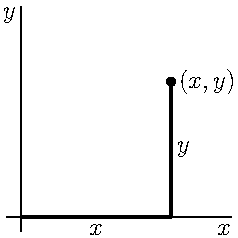
\includegraphics{point2d.pdf}
\end{center}
\end{efig}
The set of all points in two dimensions is denoted\footnote{Not surprisingly,
the $2$ in $\bbbr^2$ signifies that each point is labelled by two numbers
and the $\bbbr$ in $\bbbr^2$ signifies that the numbers in question are
real numbers. There are more advanced applications (for example in
signal analysis and in quantum mechanics) where complex numbers are used.
The space of all pairs $(z_1,z_2)$, with $z_1$ and $z_2$ complex numbers 
is denoted  $\bbbc^2$.} $\bbbr^2$.
Observe that 
\begin{itemize}\itemsep1pt \parskip0pt \parsep0pt
\item the distance from the point $(x,y)$ to the $x$-axis is $|y|$
\item if $y>0$, then $(x,y)$ is above the $x$-axis and if $y<0$, then
        $(x,y)$ is below the $x$-axis
\item the distance from the point $(x,y)$ to the $y$-axis is $|x|$
\item if $x>0$, then $(x,y)$ is the right of the $y$-axis and if $x<0$, then
        $(x,y)$ is to the left of the $y$-axis
\item the distance from the point $(x,y)$ to the origin $(0,0)$ is 
     $\sqrt{x^2+y^2}$
\end{itemize}

Similarly, each point in three dimensions may be labeled by 
three coordinates $(x,y,z)$, as in the two figures below.
\begin{efig}
\begin{center}
   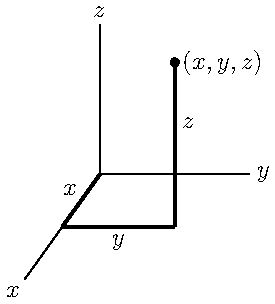
\includegraphics{point3d.pdf}\qquad
   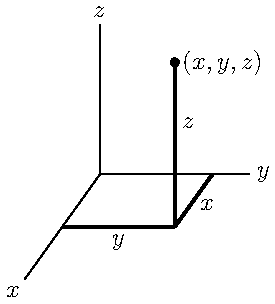
\includegraphics{point3db.pdf}
\end{center}
\end{efig}
The set of all points in three dimensions is denoted $\bbbr^3$.
The plane that contains, for example, the $x$- and $y$-axes
is called the $xy$-plane.
\begin{itemize}\itemsep1pt \parskip0pt \parsep0pt
\item The $xy$-plane is the set of all points $(x,y,z)$ that
satisfy $z=0$.
\item The $xz$-plane is the set of all points $(x,y,z)$ that
satisfy $y=0$.
\item The $yz$-plane is the set of all points $(x,y,z)$ that
satisfy $x=0$.
\end{itemize}
More generally,
\begin{itemize}\itemsep1pt \parskip0pt \parsep0pt
\item The set of all points $(x,y,z)$ that obey $z=c$ is a plane
that is parallel to the $xy$-plane and is a distance $|c|$ from it. 
If $c>0$, the plane $z=c$ is above the $xy$-plane.
If $c<0$, the plane $z=c$ is below the $xy$-plane.
We say that the plane $z=c$ is a signed distance $c$ from the
$xy$-plane.

\item The set of all points $(x,y,z)$ that obey $y=b$ is a plane
that is parallel to the $xz$-plane and is a signed distance $b$ from it. 

\item The set of all points $(x,y,z)$ that obey $x=a$ is a plane
that is parallel to the $yz$-plane and is a signed distance $a$ from it. 
\end{itemize}
\begin{efig}
\begin{center}
   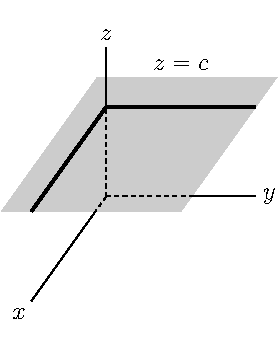
\includegraphics[scale=0.75]{xyplaneN.pdf}\qquad
   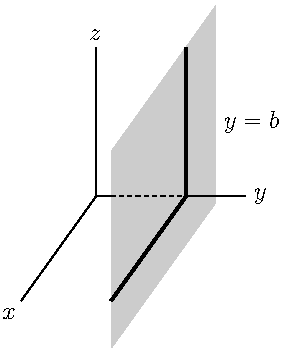
\includegraphics[scale=0.75]{xzplaneN.pdf}\qquad
   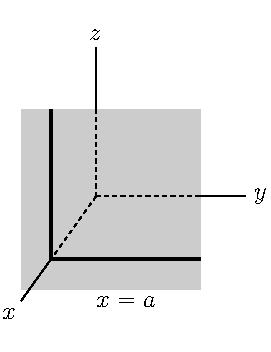
\includegraphics[scale=0.75]{yzplaneN.pdf}
\end{center}
\end{efig}
Observe that our 2d distances extend quite easily to 3d.
\begin{itemize}\itemsep1pt \parskip0pt \parsep0pt
\item the distance from the point $(x,y,z)$ to the $xy$-plane is $|z|$
\item the distance from the point $(x,y,z)$ to the $xz$-plane is $|y|$
\item the distance from the point $(x,y,z)$ to the $yz$-plane is $|x|$
\item the distance from the point $(x,y,z)$ to the origin $(0,0,0)$ is 
     $\sqrt{x^2+y^2+z^2}$
\end{itemize}
To see that the distance from the point $(x,y,z)$ to the origin $(0,0,0)$ 
is indeed  $\sqrt{x^2+y^2+z^2}$,
\begin{itemize}\itemsep1pt \parskip0pt \parsep0pt
\item 
apply Pythagoras to the right-angled triangle with vertices $(0,0,0)$,
$(x,0,0)$ and $(x,y,0)$ to see that the distance from $(0,0,0)$
to $(x,y,0)$ is $\sqrt{x^2+y^2}$ and then
\item 
apply Pythagoras to the right-angled triangle with vertices $(0,0,0)$,
$(x,y,0)$ and $(x,y,z)$ to see that the distance from $(0,0,0)$
to $(x,y,z)$ is $\sqrt{{\big(\sqrt{x^2+y^2}\big)}^2+z^2}
=\sqrt{x^2+y^2+z^2}$.
\end{itemize}
\begin{efig}
\begin{center}
   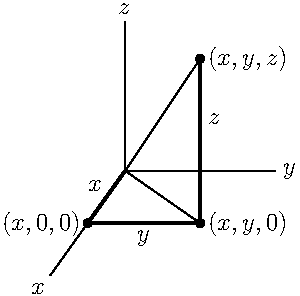
\includegraphics{pythag3d.pdf}
\end{center}
\end{efig}
More generally, the distance from the point $(x,y,z)$ to the point 
$(x',y',z')$ is
\begin{equation*}
\sqrt{(x-x')^2+(y-y')^2+(z-z')^2}
\end{equation*}
Notice that this gives us the equation for a sphere quite directly. 
All the points on a sphere are equidistant from the centre of the sphere.
So, for example, the equation of the sphere centered on $(1,2,3)$ with 
radius $4$, that is, the set of all points $(x,y,z)$ whose distance 
from $(1,2,3)$ is $4$, is 
\begin{equation*}
(x-1)^2+(y-2)^2+(z-3)^2=16
\end{equation*}

Here is an example in which we sketch a region in the $xy$-plane that is specified using inequalities.

\begin{eg}
In this example, we sketch the region
\begin{equation*}
\Set{(x,y)}{ -12\le x^2-6x +y^2-4y \le -9,\ \ y\ge 1}
\end{equation*}
in the $xy$-plane.

We do so in two steps. In the first step, we sketch the curves
$x^2-6x +y^2-4y=-12$, $x^2-6x +y^2-4y=-9$, and $y=1$.
\begin{itemize}
\item
By completing squares, we see that the equation  $x^2-6x +y^2-4y=-12$ 
is equivalent to $(x-3)^2 +(y-2)^2 =1$, which is the circle of radius 
$1$ centred on $(3,2)$. It is sketched in the figure below.

\item
By completing squares, we see that the equation  $x^2-6x +y^2-4y=-9$ 
is equivalent to $(x-3)^2 +(y-2)^2 =4$, which is the circle of radius 
$2$ centred on $(3,2)$. It is sketched in the figure below.

\item
The point $(x,y)$ obeys $y=1$ if and only if it is a distance $1$ vertically above the $x$-axis. So $y=1$ is the line that is parallel to the $x$-axis and is one unit above it. This line is also  sketched in the figure below.
\end{itemize}

\begin{efig}
\begin{center}
   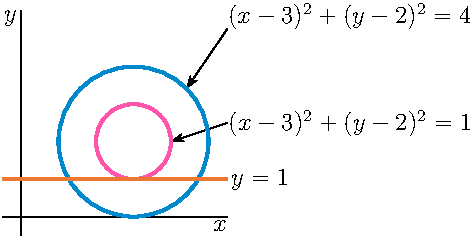
\includegraphics{annulusPart.pdf}
\end{center}
\end{efig}

In the second step we determine the impact that the inequalities have.
\begin{itemize}
\item 
The inequality $x^2-6x +y^2-4y\ge -12$ is equivalent to 
$(x-3)^2 +(y-2)^2 \ge 1$ and hence is equivalent to 
$\sqrt{(x-3)^2 +(y-2)^2} \ge 1$. So the point $(x,y)$ satisfies  
$x^2-6x +y^2-4y\ge -12$ if and only if the distance from $(x,y)$ to $(3,2)$
is at least $1$, i.e. if and only if $(x,y)$ is outside (or on) the circle 
$(x-3)^2 +(y-2)^2 = 1$. 

\item 
The inequality $x^2-6x +y^2-4y\le -9$ is equivalent to 
$(x-3)^2 +(y-2)^2 \le 4$ and hence is equivalent to 
$\sqrt{(x-3)^2 +(y-2)^2} \le 2$. So the point $(x,y)$ satisfies the inequality 
$x^2-6x +y^2-4y\le -9$ if and only if the distance from $(x,y)$ to $(3,2)$
is at most $2$, i.e. if and only if $(x,y)$ is inside (or on) the circle 
$(x-3)^2 +(y-2)^2 = 4$. 

\item 
The point $(x,y)$ obeys $y\ge 1$ if and only if $(x,y)$ is a vertical distance at least $1$ above the $x$-axis, i.e. is above (or on) the line $y=1$.

\item
So the region  
\begin{equation*}
\Set{(x,y)}{ -12\le x^2-6x +y^2-4y \le -9,\ \ y\ge 1}
\end{equation*}
consists of all points $(x,y)$ that 
\begin{itemize}
\item 
are inside or on the circle $(x-3)^2 +(y-2)^2 = 4$ and 
\item 
are also outside or on the circle $(x-3)^2 +(y-2)^2 = 1$ and 
\item 
are also above or on the line $y=1$. 
\end{itemize}
It is the shaded region in the figure below.
\end{itemize}

\begin{efig}
\begin{center}
   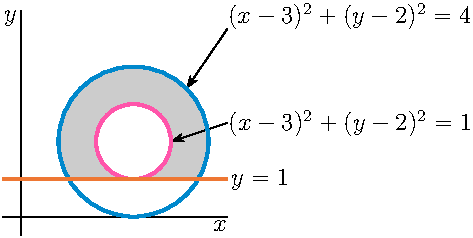
\includegraphics{annulusPartB.pdf}
\end{center}
\end{efig}

\end{eg}

Here are a couple of examples that involve spheres.

\begin{eg}
In this example, we are going to find the curve formed by the intersection of the $xy$-plane and the sphere of radius $5$ centred on $(0,0,4)$. 

The point $(x,y,z)$ lies on the $xy$-plane if and only if $z=0$, and lies on the  
sphere of radius $5$ centred on $(0,0,4)$ if and only if
$x^2+y^2+(z-4)^2=25$. So the point $(x,y,z)$ lies on the curve of intersection if and only if both $z=0$ and $x^2+y^2+(z-4)^2=25$, or equivalently
\begin{equation*}
z=0,\quad x^2+y^2+(0-4)^2=25
\iff
z=0,\quad x^2+y^2 = 9
\end{equation*}
This is the circle in the $xy$-plane that is centred on the origin and
has radius $3$. Here is a sketch that show the parts of the sphere 
and the circle of intersection that are in the first octant. That is, that
have $x\ge 0$, $y\ge 0$ and $z\ge 0$.
\begin{efig}
\begin{center}
   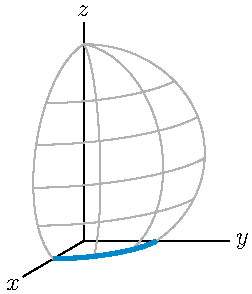
\includegraphics{sphereCircle.pdf}
\end{center}
\end{efig}
\end{eg}

\begin{eg}
In this example, we are going to find all points $(x,y,z)$ for which
the distance from $(x,y,z)$ to $(9,-12,15)$ is twice the distance from $(x,y,z)$   to the origin $(0,0,0)$.

The distance from $(x,y,z)$ to $(9,-12,15)$ is 
$\sqrt{(x-9)^2+(y+12)^2+(z-15)^2}$.
The distance from $(x,y,z)$ to $(0,0,0)$ is 
$\sqrt{x^2+y^2+z^2}$. So we want to find all points $(x,y,z)$ for which
\begin{equation*}
\sqrt{(x-9)^2+(y+12)^2+(z-15)^2}
=2\sqrt{x^2+y^2+z^2}
\end{equation*}
Squaring both sides of this equation gives
\begin{align*}
x^2-18x+81 +y^2+24y+144 +z^2-30z+225 &= 4\big(x^2+y^2+z^2)
\end{align*}
Collecting up terms gives
\begin{align*}
3x^2+18x +3y^2-24y +3z^2+30z &= 450\qquad\text{and then, dividing by $3$,} \\
x^2+6x +y^2-8y +z^2+10z &= 150\qquad\text{and then, completing squares,} \\
x^2+6x +9 +y^2-8y +16  +z^2+10z +25 &= 200\qquad\text{or}\\
(x+3)^2+(y-4)^2+(z+5)^2 =200 
\end{align*}
This is the sphere of radius $10\sqrt{2}$ centred on $(-3,4,-5)$.
\end{eg}

%%%%%%%%%%%%%%%%%%%%%%%%
\section{Vectors}\label{sec vectors}
%%%%%%%%%%%%%%%%%%%%%%%%%
In many of our applications in 2d and 3d, we will encounter quantities
that have both a magnitude (like a distance) and also a 
direction. Such quantities are called vectors. That is,
a \emph{vector} is a quantity which has both a direction and a magnitude,
like a velocity. If you are moving, the magnitude (length) of your 
velocity vector is your speed (distance travelled per unit time)  and the
direction of your velocity vector is your direction of motion. To specify 
a vector in three dimensions you have to give three components, just as for 
a point. To draw the vector with components $\ a,\ b,\ c\ $ you can draw 
an arrow from the point $(0,0,0)$ to the point $(a,b,c)$. 
\vadjust{
      \begin{efig} 
      \begin{center}
      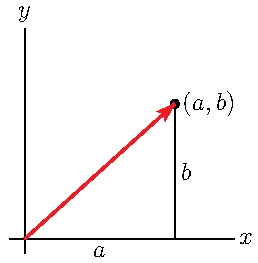
\includegraphics{vector2d.pdf} \qquad\qquad
      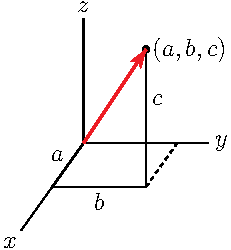
\includegraphics{vector3d.pdf}
      \end{center}
      \end{efig}
        }%
Similarly, to specify a vector in two dimensions
you have to give two components and to draw the vector
with components $\ a,\ b\ $ you can draw an arrow from the point $(0,0)$
to the point $(a,b)$.

There are many situations in which it is preferable to draw a vector 
with its tail at some point other than the origin. For example, it is 
natural to draw the velocity vector of a moving particle with the tail
of the velocity vector at the position of the particle, whether or not
the particle is at the origin. The sketch below shows a moving particle
and its velocity vector at two different times.
      \begin{efig} 
      \begin{center}
      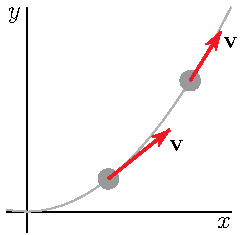
\includegraphics{movingParticle.pdf}
      \end{center}
      \end{efig}
As a second example, suppose that you are analyzing the motion of a pendulum.
There are three forces acting on the pendulum bob: gravity $\vg$, which
is pulling the bob straight down, tension $\vt$ in the rod, which is
pulling the bob in the direction of the rod, and air resistance $\vr$, 
which is pulling the bob in a direction opposite to its direction of motion.
All three forces are acting on the bob. So it is natural to draw all three
arrows representing the forces with their tails at the bob. 
      \begin{efig} 
      \begin{center}
      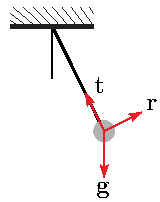
\includegraphics{pendulum.pdf}
      \end{center}
      \end{efig}

In this text, we will used bold faced letters, like $\vv$, $\vt$, $\vg$,
to designate vectors. In handwriting, it is clearer to use a small 
overhead arrow\footnote{Some people use an underline, as in $\underline{v}$,
rather than an arrow.}, as in $\vec{v}$, $\vec{t}$, $\vec{g}$, instead. 
Also, when we want to emphasise that some quantity is a number,
rather than a vector, we will call the number a \emph{scalar}. 


Both points and vectors in 2d are specified by two numbers. Until 
you get used to this, it might confuse you sometimes --- does a given pair of 
numbers represent a point or a vector?
To distinguish\footnote{Or, in the Wikipedia jargon, disambiguate.}
between the components of a vector and the coordinates 
of the point at its head, when its tail is at some point other than 
the origin, we shall use angle brackets rather than round brackets 
around the components of a vector. For example, the figure below shows 
the two-dimensional vector $\llt 2,1\rgt$ drawn in three different positions.
In each case, when the tail is at the point $(u,v)$ the head is at 
$(2+u,1+v)$. We warn you that, out in the  real world\footnote{OK. OK. Out in 
that (admittedly very small) part of the real world that actually knows 
what a vector is.}, no one uses notation
that distinguishes between components of a vector and the coordinates of its 
head --- usually round brackets are used for both. It is up to you to 
keep straight which is being referred to.

\begin{efig}
  \begin{center}
  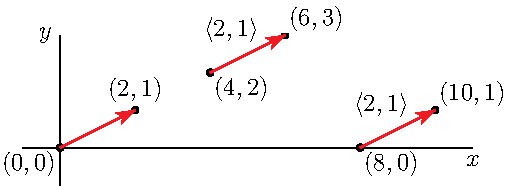
\includegraphics{positions.pdf}
  \end{center}
\end{efig}

By way of summary, 
\begin{notn}\label{not scalar vector}
we use
\begin{itemize}\itemsep1pt \parskip0pt \parsep0pt
\item
bold faced letters, like $\vv$, $\vt$, $\vg$, to designate vectors,
and
\item
angle brackets, like $\llt 2,1\rgt$, around the components of a vector,
but use
\item
round brackets, like $(2,1)$, around the coordinates of a point,
and use
\item ``scalar'' to emphasise that some quantity is a number,
rather than a vector.
\end{itemize}
\end{notn}

%%%%%%%%%%
\subsection{Addition of Vectors and Multiplication of a Vector by a Scalar}
%%%%%%%%%

Just as we have done many times in the CLP texts, when we define a new 
type of object, we want to understand how it interacts with the basic 
operations of addition and multiplication. Vectors are no different, and 
we shall shortly see a natural way to define addition of vectors.
Multiplication will be more subtle, and we shall start with multiplication of a vector by a number (rather than with multiplication of a vector by 
another vector).

By way of motivation for the definitions of addition and multiplication by a number, imagine that we are out for a walk on the $xy$-plane. 
\begin{itemize}
\item 
Suppose that we take a step and, in doing so, we move $a_1$ units parallel to the $x$-axis and $a_2$ units parallel to the $y$-axis. 
Then we say that $\llt a_1, a_2\rgt$ is the displacement vector for the step. Suppose now that we take a second step which moves us an additional $b_1$ units  parallel to the $x$-axis and an additional $b_2$ units  parallel to the $y$-axis, as in the figure on the left below. So the displacement 
vector for the second step is $\llt b_1, b_2\rgt$. All together, we have moved $a_1+b_1$ units  parallel to the $x$-axis and $a_2+b_2$ units parallel to the $y$-axis. The displacement vector for the two steps combined is  
$\llt a_1+b_1, a_2+b_2\rgt$. We shall define
the sum of $\llt a_1, a_2\rgt$ and $\llt b_1, b_2\rgt$, denoted by
$\llt a_1, a_2\rgt+\llt b_1,b_2\rgt$, to be $\llt a_1+b_1, a_2+b_2\rgt$.

\item
Suppose now that, instead, we decide to step in the same direction
as the first step above, but to move twice as far, as in the figure on the right below. That is, our step will move us $2a_1$ units in the direction of the $x$-axis and $2a_2$ units in the direction of the $y$-axis and the 
corresponding displacement vector will be $\llt 2a_1, 2a_2\rgt$. 
We shall define the product of the number $2$ and the vector
$\llt a_1, a_2\rgt$, denoted by $2\llt a_1, a_2\rgt$, to be 
$\llt 2a_1, 2a_2\rgt$.
\end{itemize}

\begin{efig}
  \begin{center}
  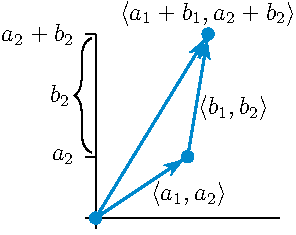
\includegraphics{maddvec.pdf}\qquad
  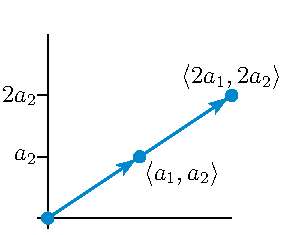
\includegraphics{mscalmul.pdf}
  \end{center}
\end{efig}

Here are the formal definitions.

\begin{defn}[Adding Vectors and Multiplying a Vector by a Number]
             \label{def:addScalMult}
These two operations have the obvious definitions
\begin{alignat*}{2}
&\va=\llt a_1,a_2\rgt,\ \vb =\llt b_1,b_2\rgt
             \qquad&&\implies\qquad\va+\vb=\llt a_1+b_1,a_2+b_2\rgt\\
&\va=\llt a_1,a_2\rgt,\ s\text{ a number}
            \qquad&&\implies\qquad s\va=\llt sa_1,sa_2\rgt
\end{alignat*}
and similarly in three dimensions.
\end{defn} 
Pictorially, you add the vector $\vb$ to the vector $\va$ 
by drawing $\vb$ with its tail at the head of $\va$ and then drawing
a vector from the tail of $\va$ to the head of $\vb$, as in the figure
on the left below. For a number $s$, we can draw the vector $s\va$, by 
just 
\begin{itemize}\itemsep1pt \parskip0pt \parsep0pt
\item
changing the vector $\va$'s length by the factor $|s|$, and,
\item
if $s<0$, reversing the arrow's direction, 
\end{itemize}
as in the other two figures below.
\begin{wfig}
  \begin{center}
  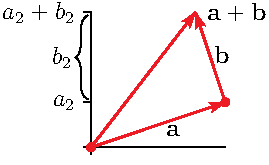
\includegraphics{addvec.pdf}\qquad\qquad
  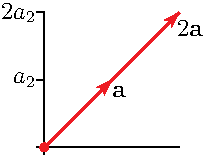
\includegraphics{scalmul.pdf}\qquad\qquad
  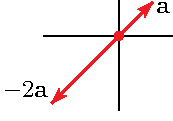
\includegraphics{negmul.pdf}
  \end{center}
\end{wfig}
The special case of multiplication by $s=-1$ appears so frequently that
$(-1)\va$ is given the shorter notation $-\va$. That is, 
\begin{equation*}
-\llt a_1,a_2\rgt=\llt -a_1,-a_2\rgt
\end{equation*}
Of course $\va+(-\va)$ is $\vZero$, the vector all of whose components
are zero. 

To subtract $\vb$ from $\va$ pictorially, 
you may add $-\vb$ (which is drawn by reversing the direction of $\vb$)
 to $\va$. Alternatively,
if you draw $\va$ and $\vb$ with their tails at a common point,
then $\va-\vb$ is the vector from the head of $\vb$ to
the head of $\va$. That is, $\va-\vb$ is the vector you
must add to $\vb$ in order to get $\va$.
\begin{efig}
  \begin{center}
  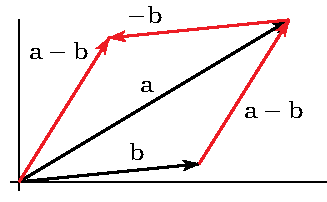
\includegraphics{subtract.pdf}
  \end{center}
\end{efig}


The operations of addition and multiplication by a scalar that we have just
defined are quite natural and rarely cause any problems, because 
they inherit from the real numbers the properties of  addition and 
multiplication that you are used to. 
\begin{theorem}[Properties of Addition and Scalar Multiplication]
                    \label{thm:addScalMult}
Let $\va$, $\vb$ and $\vc$ be vectors and $s$ and $t$ be scalars. Then 
\begin{alignat*}{5}
& (1)\quad&&\va+\vb=\vb+\va \qquad\qquad\qquad
&& (2)\quad&&\va+(\vb+\vc)=(\va+\vb)+\vc\\
& (3) &&\va+\vZero =\va 
&& (4) &&\va+(-\va)=\vZero\\
& (5) &&s(\va+\vb)=s\va+s\vb
&& (6) &&(s+t)\va=s\va+t\va\\
& (7) &&(st)\va = s(t\va)
&& (8) &&1\va=\va\\
\end{alignat*}
\end{theorem}

\noindent We have just been introduced to many definitions. Let's
see some of them in action.
\begin{eg}
For example, if 
\begin{equation*}
\va = \llt 1,2,3\rgt\qquad
\vb = \llt 3,2,1\rgt\qquad
\vc = \llt 1,0,1\rgt
\end{equation*}
then
\begin{alignat*}{3}
2\va&=2\llt 1,2,3\rgt&&=\llt 2,4,6\rgt \\
-\vb&=-\llt 3,2,1\rgt&&=\llt -3,-2,-1\rgt \\
3\vc&=3\llt 1,0,1\rgt&&=\llt 3,0,3\rgt
\end{alignat*}
and 
\begin{align*}
2\va-\vb+3\vc 
&= \llt 2,4,6\rgt + \llt -3,-2,-1\rgt+\llt 3,0,3\rgt \\
&= \llt 2-3+3\,,\,4-2+0\,,\,6-1+3\rgt \\
&= \llt 2,2,8 \rgt
\end{align*}
\end{eg}\goodbreak

\begin{defn}\label{def parallel vectors}
Two vectors $\va$ and $\vb$
\begin{itemize}
\item
are said to be parallel if $\ \va= s\,\vb\ $ for some nonzero real number $s$ and
\item
are said to have the same direction if $\ \va=s\,\vb\ $ for some number $s>0$.
\end{itemize} 
\end{defn}


There are some vectors that occur sufficiently commonly that they are
given special names. One is the vector $\vZero$. Some others are the 
``standard basis vectors''.
\begin{defn}\label{def basis vectors}
\begin{enumerate}[(a)]
\item
The standard basis vectors in two dimensions are
\begin{align*}
\\[-0.1in]
\hi = \llt 1,0\rgt \qquad\qquad\hj =\llt 0,1\rgt \qquad\qquad
\smash{\raisebox{-0.5\height}{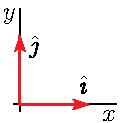
\includegraphics{basis2d.pdf}}}\\[-0.1in]
\end{align*} 
\item
The standard basis vectors in three dimensions are
\begin{align*}
\\[-0.1in]
\hi = \llt 1,0,0\rgt \qquad\qquad\hj =\llt 0,1,0\rgt 
\qquad\qquad\hk =\llt 0,0,1\rgt \qquad\quad
\smash{\raisebox{-0.25\height}{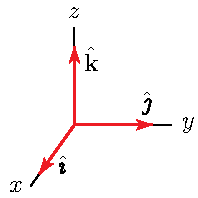
\includegraphics{basis3d.pdf}}}\\[-0.1in]
\end{align*}
\end{enumerate} 
\end{defn}
We'll explain the little hats in the notation $\hi$, $\hj$, $\hk$ shortly.
Some people rename $\hi$, $\hj$ and $\hk$ to $\he_1$, $\he_2$ and 
$\he_3$ respectively.
Using the above properties we have, for all vectors,
\begin{equation*}
\llt a_1,a_2\rgt =a_1\,\hi+a_2\,\hj\qquad\qquad
\llt a_1,a_2,a_3\rgt =a_1\,\hi+a_2\,\hj+a_3\,\hk
\end{equation*}
A sum of numbers times vectors, like $a_1\hi+a_2\hj$ is called
a linear combination of the vectors.
Thus all vectors can be expressed as linear combinations of the standard
basis vectors. This makes basis vectors very helpful in computations.
The  standard basis vectors are unit vectors, meaning that they are of 
length one, where the length of a vector $\va$ is denoted\footnote{The notation $\|\va\|$ is also used for the length of $\va$.} $|\va|$ 
and is defined by
\begin{defn}[Length of a Vector]\label{def:vectLen}
\begin{alignat*}{5}
&\va=\llt a_1,a_2\rgt \qquad&&\implies\qquad &&|\va|=\sqrt{a_1^2+a_2^2}\\
&\va=\llt a_1,a_2,a_3\rgt \qquad&&\implies\qquad &&|\va|=\sqrt{a_1^2+a_2^2+a_3^2}
\end{alignat*}
A unit vector is a vector of length one. We'll sometimes use the accent 
$\hat{\ }$ to emphasise that the vector $\hat\va$ is a unit vector.
That is, $|\hat\va|=1$.
\end{defn}


\begin{eg}\label{eg unit vector}
Recall that multiplying a vector $\va$ by a positive number $s$,
changes the length of the vector by a factor $s$ without changing
the direction of the vector. So (assuming that $|\va|\ne 0)$
$\frac{\va}{|\va|}$ is a unit vector that has the same direction as
$\va$. For example, $\frac{\llt 1,1,1\rgt}{\sqrt{3}}$ is a unit vector
that points in the same direction as $\llt 1,1,1\rgt$.
\end{eg}
\goodbreak

\begin{eg}\label{eg walk}
We go for a walk on a flat Earth. We use a coordinate system
with the positive x-axis pointing due east and the positive y-axis pointing due
north. We  
\begin{itemize}\itemsep1pt \parskip0pt \parsep0pt
\item
start at the origin and
\item 
walk due east for 4 units and then
\item 
walk northeast for $5\sqrt{2}$ units and then
\item 
head towards the point $(0,11)$, but we only go
\item
one third of the way.
\end{itemize}
      \begin{efig} 
      \begin{center}
      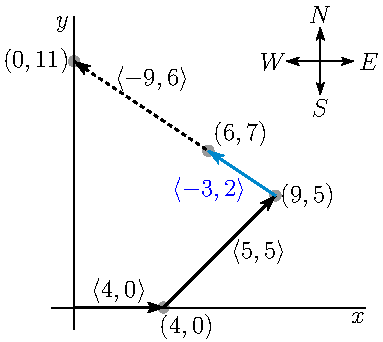
\includegraphics{addSubtractMult.pdf}\qquad\qquad
      \raisebox{0.65\height}{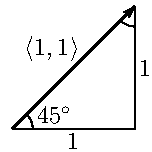
\includegraphics{triangleWalk.pdf}}
      \end{center}
      \end{efig}
We will now use vectors to figure out our final location.
\begin{itemize}\itemsep1pt \parskip0pt \parsep0pt
\item
On the first leg of our walk, we go 4 units in the positive $x$-direction.
So our displacement vector --- the vector whose tail is at our starting point and whose head is at the end point of the first leg --- is $\llt 4,0\rgt$. 
As we started at $(0,0)$ we finish the first leg of the walk at $(4,0)$.
\item
On the second leg of our walk, our direction of motion is northeast. i.e. is
$45^\circ$ above the direction of the positive $x$-axis. Looking at the figure 
on the right above, we see that our displacement vector, for the second leg of the walk, has to be in the same direction as the vector $\llt 1,1\rgt$.
So our displacement vector is the vector of length $5\sqrt{2}$ with the same direction as $\llt 1,1\rgt$. The vector $\llt 1,1\rgt$ has length
$\sqrt{1^2+1^2}=\sqrt{2}$ and so $\frac{\llt 1,1\rgt}{\sqrt{2}}$ has length one
and our displacement vector is
\begin{equation*}
5\sqrt{2}\ \frac{\llt 1,1\rgt}{\sqrt{2}}
=5 \llt 1,1\rgt 
=\llt 5,5\rgt
\end{equation*}
If we draw this displacement vector, $\llt 5,5\rgt$ with its tail at 
$(4,0)$, the starting point of the second leg of the walk, then its head 
will be at $(4+5, 0+5)=(9,5)$ and that is the end point of the second 
leg of the walk.
\item
On the final leg of our walk, we start at $(9,5)$ and walk towards $(0,11)$.
The vector from $(9,5)$ to $(0,11)$ is $\llt 0-9\,,\,11-5\rgt =\llt -9,6\rgt$.
As we go only one third of the way, our final displacement vector is
\begin{equation*}
\frac{1}{3}\llt -9,6\rgt
=\llt -3,2\rgt
\end{equation*}
If we draw this displacement vector with its tail at 
$(9,5)$, the starting point of the final leg, then its head 
will be at $(9-3, 5+2)=(6,7)$ and that is the end point of the final
leg of the walk, and our final location.
\end{itemize}
\end{eg}

%%%%%%%%%%%%%%%%%%%%%%%%%%%%%%%%%%%%%%%%%%%%%%%%%%%%%%%%%%%
\subsection{The Dot Product}\label{subsec dot product}
%%%%%%%%%%%%%%%%%%%%%%%%%%%%%%%%%%%%%%%%%%%%%%%%%%%%%%%%%%%
Let's get back to the arithmetic operations of addition and multiplication.
We will be using both scalars and vectors. So, for each operation there are 
three possibilities that we need to explore: 
\begin{itemize}\itemsep1pt \parskip0pt \parsep0pt
\item ``scalar plus scalar'', ``scalar plus vector'' and ``vector plus vector''
\item``scalar times scalar'', ``scalar times vector'' and 
         ``vector times vector''
\end{itemize}
We have been using ``scalar plus scalar'' and ``scalar times scalar''
since childhood. ``vector plus vector'' and ``scalar times vector''
were just defined above. There is no sensible way to define ``scalar plus vector'', so we won't. This leaves ``vector times vector''. 
There are actually two widely used such products.
The first is the \emph{dot product}, which is the topic of this section,
and which is used to easily determine the angle $\theta$ (or more precisely,
$\cos\theta$) between two vectors.
We'll get to the second, the cross product, later. 

Here is preview of what we will do in this dot product 
subsection \S\ref{subsec dot product}. We are going to give two formulae
for the dot product, $\va\cdot\vb$, of the pair of vectors 
$\va=\llt a_1,a_2,a_3\rgt$ and $\vb=\llt b_1,b_2,b_3\rgt$.
\begin{itemize}
\item 
The first formula is $\va\cdot\vb = a_1b_1+a_2b_2+a_3b_3$.
We will take it as our official definition of $\va\cdot\vb$.
This formula provides us with an easy way to compute dot products.

\item
The second formula is $\va\cdot\vb=|\va|\,|\vb|\,\cos\theta$, 
        where $\theta$ is the angle between $\va$ and $\vb$.
      \begin{efig} 
      \begin{center}
      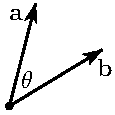
\includegraphics{dotAngle.pdf}
      \end{center}
      \end{efig}
We will show, in Theorem \ref{thm:dotPppties} below, that this second formula always gives the same answer as the first formula.
The second formula provides us with an easy way to determine the angle between two vectors. In particular, it provides us with an easy way to test whether or not two vectors are perpendicular to each other. For example,
the vectors $\llt 1,2,3\rgt$ and $\llt -1,-1,1\rgt$ have dot product
\begin{equation*}
\llt 1,2,3\rgt\cdot\llt -1,-1,1\rgt = 1\times(-1)+2\times(-1)+3\times 1=0
\end{equation*}
This tell us as the angle $\theta$ between the two vectors obeys 
$\cos\theta=0$, so that $\theta=\frac{\pi}{2}$. That is, the two vectors are perpendicular to each other.
\end{itemize}
After we give our official definition of the dot product in
Definition \ref{def:dotProd}, and give the important properties of the dot product, including the formula  $\va\cdot\vb=|\va|\,|\vb|\,\cos\theta$,
in Theorem \ref{thm:dotPppties}, we'll give some examples.
Finally, to see the dot product in action, we'll define what it means to 
project one vector on another vector and give an example.

\begin{defn}[Dot Product]\label{def:dotProd}
The dot product of the vectors $\va$ and $\vb$ is denoted $\va\cdot\vb$ 
and is defined by
\begin{alignat*}{5}
&\va=\llt a_1,a_2\rgt ,\quad &&\vb=\llt b_1,b_2\rgt\quad &\implies\quad
&\va\cdot\vb = a_1b_1+a_2b_2\\
&\va=\llt a_1,a_2,a_3\rgt ,\quad &&\vb=\llt b_1,b_2,b_3\rgt\quad &\implies\quad
&\va\cdot\vb = a_1b_1+a_2b_2+a_3b_3
\end{alignat*}
in two and three dimensions respectively. 
\end{defn}
The properties of the dot 
product are as follows:
\begin{theorem}[Properties of the Dot Product]\label{thm:dotPppties}
Let $\va$, $\vb$ and $\vc$ be vectors and let $s$ be a scalar. Then
\begin{alignat*}{3}
&(0)\quad &&\va,\vb\text{ are vectors and }\va\cdot\vb
              \text{ is a scalar}\\
&(1) &&\va\cdot\va=|\va|^2\\
&(2) &&\va\cdot\vb=\vb\cdot\va\\
&(3) &&\va\cdot(\vb+\vc)=\va\cdot\vb+\va\cdot\vc,\quad 
       (\va+\vb)\cdot\vc=\va\cdot\vc+\vb\cdot\vc\\
&(4) &&(s\va)\cdot\vb= s(\va\cdot\vb)\\
&(5)  &&\vZero \cdot\va=0\\
&(6) &&\va\cdot\vb=|\va|\,|\vb|\,\cos\theta
        \text{ where $\theta$ is the angle between $\va$ and $\vb$}\\
&(7) &&\va\cdot\vb=0\iff \va=\vZero \text{ or }\vb=\vZero 
    \text{ or } \va\perp\vb
\end{alignat*}
\end{theorem}
\begin{proof}
Properties 0 through 5 are almost immediate consequences of the definition.
For example, for property 3 (which is called the distributive law)
in dimension 2,
\begin{align*}
\va\cdot(\vb+\vc)
    &=\llt a_1,a_2\rgt \cdot\llt b_1+c_1,b_2+c_2\rgt \\
    &=a_1(b_1+c_1)+a_2(b_2+c_2)=a_1b_1+a_1c_1+a_2b_2+a_2c_2\\
\va\cdot\vb+\va\cdot\vc
&=\llt a_1,a_2\rgt \cdot\llt b_1,b_2\rgt 
             +\llt a_1,a_2\rgt \cdot\llt c_1,c_2\rgt \\
&=a_1b_1+a_2b_2+a_1c_1+a_2c_2
\end{align*}


Property 6 is sufficiently important that it is often used as the 
definition of dot product. It is not at all an obvious consequence of the definition.
To verify it, we just write $|\va-\vb|^2$ in two different ways. 
The first expresses $|\va-\vb|^2$ in terms of $\va\cdot\vb$. 
It is
\begin{align*}
|\va-\vb|^2\ &{\buildrel 1 \over =}\ (\va-\vb\,)\cdot(\va-\vb\,)\\
&{\buildrel 3 \over =}\ \va\cdot\va-\va\cdot\vb-\vb\cdot\va
+\vb\cdot\vb\\
&{\buildrel 1,2 \over =}\ |\va|^2+|\vb|^2-2\va\cdot\vb
\end{align*}
Here, ${\buildrel 1 \over =}$, for
example, means that the equality is  a consequence of property 1.
The second way we write $|\va-\vb|^2$ involves $\cos\theta$ and follows from
the cosine law for triangles. Just in case you don't remember the 
cosine law, we'll derive it right now! Start by applying Pythagoras to the 
shaded triangle in the right hand figure of

      \begin{efig} 
      \begin{center}
      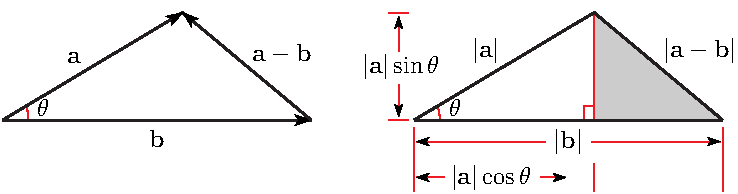
\includegraphics{cosineB.pdf}
      \end{center}
      \end{efig}
That triangle is a right triangle whose hypotenuse has length $|\va-\vb|$ 
and  whose other two sides have lengths $\big(|\vb|-|\va|\cos\theta\big)$ 
and $|\va|\sin\theta$. So Pythagoras gives
\begin{align*}
|\va-\vb|^2&=\big(|\vb|-|\va|\cos\theta\big)^2+
\big(|\va|\sin\theta\big)^2\\
&=|\vb|^2-2|\va|\,|\vb|\,\cos\theta+|\va|^2\cos^2\theta
+|\va|^2\sin^2\theta\\
&=|\vb|^2-2|\va|\,|\vb|\,\cos\theta+|\va|^2
\end{align*}
This is precisely the cosine law\footnote{You may be used to seeing it written as $c^2=a^2+b^2-2 a b \cos C$, where $a$, $b$ and $c$ are the lengths of the 
three sides of the triangle and $C$ is the angle opposite the side of length $c$}. 
Observe that, when $\theta=\tfrac{\pi}{2}$, 
this reduces to, (surprise!) Pythagoras' theorem.

Setting our two expressions for $|\va-\vb|^2$ equal to each other,
\begin{align*}
|\va-\vb|^2=|\va|^2+|\vb|^2-2\va\cdot\vb
=|\vb|^2-2|\va|\,|\vb|\,\cos\theta+|\va|^2
\end{align*}
cancelling the $|\va|^2$ and $|\vb|^2$ common to both sides
\begin{align*}
-2\va\cdot\vb
=-2|\va|\,|\vb|\,\cos\theta
\end{align*}
and dividing by $-2$ gives 
\begin{align*}
\va\cdot\vb=|\va|\,|\vb|\,\cos\theta
\end{align*}
which is exactly property 6. 


Property 7 follows directly from property 6. First note that the dot product $\va\cdot\vb=|\va|\,|\vb|\,\cos\theta$
is zero if and only if at least one of the three factors 
$|\va|,\ |\vb|,\ \cos\theta$ is zero. The first factor is zero if
and only if $\va=\vZero $. The second factor is zero if and only if 
$\vb=\vZero $.
The third factor is zero if and only if $\theta=\pm\tfrac{\pi}{2}+2k\pi$,
for some integer $k$, which in turn is true if and only if $\va$ and 
$\vb$ are mutually perpendicular.
\end{proof}
Because of Property 7 of Theorem \ref{thm:dotPppties}, the dot product 
can be used to test whether or not two vectors are perpendicular to 
each other. That is, whether or not the angle between the two vectors 
is $90^\circ$. Another name\footnote{The concepts of the dot product
and perpendicularity have been generalized a lot in mathematics (for example,
from 2d and 3d vectors to functions). The generalization of the dot 
product is called the ``inner product'' and the generalization 
of perpendicularity is called ``orthogonality''.} for ``perpendicular'' 
is ``orthogonal''. Testing for orthogonality is one of the main uses of the
dot product. 

\begin{eg}
Consider the three vectors
\begin{equation*}
\va=\llt 1,1,0 \rgt\qquad
\vb=\llt 1,0,1 \rgt \qquad
\vc=\llt -1,1,1\rgt
\end{equation*}
Their dot products
\begin{alignat*}{3}
\va\cdot\vb & = \llt 1,1,0 \rgt \cdot \llt 1,0,1 \rgt
           && = 1\times 1 +1\times 0+0\times 1
           && = 1 \\
\va\cdot\vc & = \llt 1,1,0 \rgt \cdot \llt -1,1,1 \rgt
           && = 1\times(-1) +1\times 1+0\times 1
           && = 0 \\
\vb\cdot\vc & = \llt 1,0,1 \rgt \cdot \llt -1,1,1 \rgt
           && = 1\times(-1) +0\times 1+1\times 1
           && = 0
\end{alignat*}
tell us that $\vc$ is perpendicular to both $\va$ and $\vb$.
Since both $|\va|=|\vb|=\sqrt{1^2+1^2+0^2}=\sqrt{2}$ the first dot product
tells us that the angle, $\theta$, between $\va$ and $\vb$ obeys
\begin{align*}
\cos\theta =\frac{\va\cdot\vb}{|\va|\,|\vb|}=\frac{1}{2}
\implies
\theta =\frac{\pi}{3}
\end{align*}

\begin{efig}
  \begin{center}
  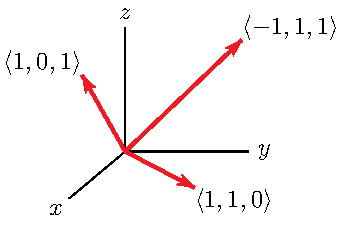
\includegraphics{dotProd.pdf}
  \end{center}
\end{efig}

\end{eg}
\goodbreak


Dot products are also used to compute projections.  First, here's
the definition.

\begin{defn}[Projection]\label{def:projection}
Draw two vectors, $\va$ and $\vb$,
with their tails at a common point and drop a perpendicular from the head of
$\va$ to the line that passes through both the head and tail of $\vb$. 
By definition, the projection of the vector $\va$
on the vector $\vb$ is the vector from the tail of $\vb$ to the point
on the line where the perpendicular hits.
      \begin{efig} 
      \begin{center}
      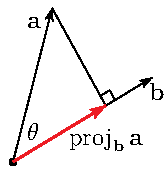
\includegraphics{projA.pdf}\qquad\qquad
      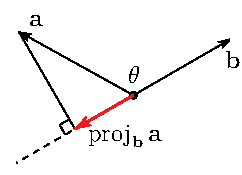
\includegraphics{projB.pdf}
      \end{center}
      \end{efig}
\end{defn}\noindent
Think of the projection of $\va$ on $\vb$ as the part of $\va$ that is in the 
direction of $\vb$.

Now let's develop a formula for the projection of $\va$ on $\vb$.
Denote by $\theta$ the angle between $\va$ and $\vb$. If $|\theta|$ is no
more than $90^\circ$, as in the figure on the left above, 
the length of the projection of $\va$ on $\vb$ is 
$|\va|\cos\theta$.
By Property 6 of Theorem \ref{thm:dotPppties},  
$|\va|\cos\theta=\va\cdot\vb/|\vb|$, so the
projection is a vector whose length is $\va\cdot\vb/|\vb|$ and
whose direction is given by the unit vector $\vb/|\vb|$. Hence
\begin{align*}
\text{projection of $\va$ on $\vb$}={\rm proj}_{\vb}\,\va
=\frac{\va\cdot\vb}{|\vb|}\frac{\vb}{|\vb|}
=\frac{\va\cdot\vb}{|\vb|^2}\,\vb
\end{align*}
If $|\theta|$ is larger than $90^\circ$, as in the figure on the right above, the projection has length 
$|\va|\,\cos(\pi-\theta)=-|\va|\cos\theta=-\va\cdot\vb/|\vb|$
 and direction $-\vb/|\vb|$. In this case
\begin{align*}
{\rm proj}_{\vb}\,\va
=-\frac{\va\cdot\vb}{|\vb|}\frac{-\vb}{|\vb|}
=\frac{\va\cdot\vb}{|\vb|^2}\ \vb
\end{align*}
So the formula 
\begin{impeqn}\label{eqn proj}
\begin{equation*}
{\rm proj}_{\vb}\,\va=\frac{\va\cdot\vb}{|\vb|^2}\,\vb
\end{equation*} 
\end{impeqn}\noindent
is applicable whenever $\vb\ne\vZero $. As a special case, if $\vb$ happens 
to be a unit vector, which, for emphasis, we'll now write has $\hat\vb$, 
the projection formula simplifies to
\begin{impeqn}\label{eqn unit proj}
\begin{align*}
{\rm proj}_{\hat\vb}\,\va
=  (\va\cdot\hat\vb)\,\hat\vb
\end{align*}
\end{impeqn}

\begin{eg}\label{eg proj}
In this example, we will find the projection of the vector $\llt 0,3\rgt$
on the vector $\llt 1,1\rgt$, as in the figure
      \begin{efig} 
      \begin{center}
      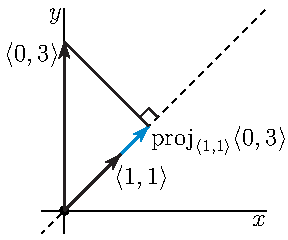
\includegraphics{projEg.pdf}
      \end{center}
      \end{efig}
By Equation \ref{eqn proj} with $\va=\llt 0,3\rgt$ and $\vb=\llt 1,1\rgt$, 
that projection is
\begin{align*}
{\rm proj}_{\llt 1,1\rgt}\,\llt 0,3\rgt
  &=\frac{\llt 0,3\rgt\cdot\llt 1,1\rgt}{|\llt 1,1\rgt|^2}\,\llt 1,1\rgt \\
  &=\frac{0\times1+3\times 1}{1^2+1^2}\,\llt 1,1\rgt
  =\llt \frac{3}{2},\frac{3}{2}\rgt
\end{align*}

\end{eg}

One use of projections is to ``resolve forces''. There is an example in
the next (optional) section.

%%%%%%%%%%%%%%%%%%%%%%%%%%%%%%%%%%%%%%%%%%%%%%%%%%%%%%%%%%%%%%%%%%%%
\subsection{(Optional) Using Dot Products to Resolve Forces
--- The Pendulum}
%%%%%%%%%%%%%%%%%%%%%%%%%%%%%%%%%%%%%%%%%%%%%%%%%%%%%%%%%%%%%%%%%%%%
Model a pendulum by a mass $m$ that is connected to a hinge by an idealized
rod that is massless and of fixed length $\ell$. Denote by $\theta$ the angle
between the rod and vertical. The forces acting on the mass are
\begin{itemize}
\item gravity, which has magnitude $mg$ and direction $\llt 0,-1\rgt$, 
\item tension in the rod, whose magnitude $\tau(t)$ automatically 
adjusts itself so that the distance between the mass and the hinge is fixed 
at $\ell$ (so that the rod does not stretch or contract) and whose 
direction is always parallel to the rod, 
\item and possibly some frictional
forces, like friction in the hinge and air resistance. Assume
that the total frictional force has magnitude proportional\footnote{The
behaviour of air resistance (sometimes called drag) is pretty complicated. 
We're using a reasonable low speed approximation. At high speeds drag is typically proportional to the square of the speed.} to the speed of the 
mass and has direction opposite to the direction of motion of the mass.
We'll call the constant of proportionality $\beta$.
\end{itemize}
      \begin{efig} 
      \begin{center}
      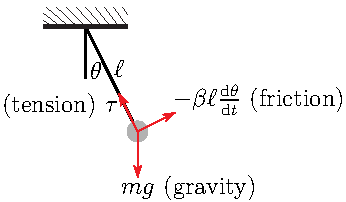
\includegraphics{pendulum3.pdf}
      \end{center}
      \end{efig}
If we use a coordinate system centered on the hinge, the $(x,y)$ coordinates
of the mass at time $t$ are 
\begin{align*}
x(t)&=\ell\sin\theta(t)\\
y(t)&=-\ell\cos\theta(t)
\end{align*}
where $\theta(t)$ is the angle between the rod and vertical at time $t$.
We are now going to use Newton's law of motion
\begin{align*}
\text{mass}\times\text{acceleration}=\text{total applied force}
\end{align*}
to determine now $\theta$ evolves in time. By definition, the
velocity and acceleration vectors\footnote{For a more comprehensive treatment 
of derivatives of vector valued functions $\vr(t)$, and in particular of
velocity and acceleration, see Section \ref{sec curves} in this text and
Section 1.1 in the CLP-4 text.} for the position vector 
$\llt x(t),y(t)\rgt$ are
\begin{align*}
\diff{}{t}\llt x(t),y(t)\rgt 
   &= \llt \diff{x}{t}(t),\diff{y}{t}(t)\rgt \\
\ddiff{2}{}{t}\llt x(t),y(t)\rgt 
   &=\llt \ddiff{2}{x}{t}(t),\ddiff{2}{y}{t}(t)\rgt 
\end{align*}
So, the velocity and acceleration vectors of our mass are
\begin{alignat*}{3}
\vv(t)&=\diff{}{t}\llt x(t),y(t)\rgt 
&&=\llt \ell\diff{}{t}\sin\theta(t),-\ell\diff{}{t}\cos\theta(t)\rgt \\
&=\llt \ell\cos\theta(t)\,\diff{\theta}{t}(t)\,,\,
             \ell\sin\theta(t)\,\diff{\theta}{t}(t)\rgt\hidewidth \\
&=\ell\,\diff{\theta}{t}(t)\,\llt \cos\theta(t),\sin\theta(t)\rgt \hidewidth
  \\[0.1in]
\va(t)&=\ddiff{2}{}{t}\llt x(t),y(t)\rgt 
&&=\diff{}{t}
  \left\{\ell\,\diff{\theta}{t}(t)\,
               \llt \cos\theta(t),\sin\theta(t)\rgt \right\} \\ 
&=\ell\,\ddiff{2}{\theta}{t}(t)\,\llt \cos\theta(t),\sin\theta(t)\rgt 
+\ell\,\diff{\theta}{t}(t)
       \llt \diff{}{t}\cos\theta(t),\diff{}{t}\sin\theta(t)\rgt \,\hidewidth\\
&= \ell\,\ddiff{2}{\theta}{t}(t)\llt \cos\theta(t),\sin\theta(t)\rgt 
+\ell \Big(\diff{\theta}{t}(t)\Big)^2
     \llt -\sin\theta(t),\cos\theta(t)\rgt\hidewidth
\end{alignat*}

The negative of the velocity vector is  
$- \ell\, \diff{\theta}{t}\llt \cos\theta,\sin\theta\rgt$, so the total frictional force is 
\begin{equation*}
-\beta\ell\, \diff{\theta}{t}\llt \cos\theta,\sin\theta\rgt 
\end{equation*} 
with $\beta$ our constant of proportionality. 

The vector 
\begin{equation*}
\tau(t) \llt -\sin\theta(t),\cos\theta(t)\rgt 
\end{equation*}
has magnitude $\tau(t)$ and direction parallel to the rod pointing 
from the mass towards the hinge and so is the force due to tension 
in the rod. 

Hence, for this physical system, Newton's law of motion is 
\begin{align}
&\overbrace{m\ell\,\ddiff{2}{\theta}{t}\llt \cos\theta,\sin\theta\rgt 
+m\ell\,\Big(\diff{\theta}{t}\Big)^2\llt -\sin\theta,\cos\theta\rgt}^
        {\text{mass}\times\text{acceleration}}
  \notag\\
&\hskip1in=
\overbrace{mg\llt 0,-1\rgt}^{\rm gravity} 
 +\overbrace{\tau \llt -\sin\theta,\cos\theta\rgt}^{\rm tension}
-\overbrace{\beta\ell\,\diff{\theta}{t}\llt \cos\theta,\sin\theta\rgt}^{\rm friction} 
\tag{$*$}
\end{align}
This is a rather complicated looking equation. Writing out its $x$- and
$y$-components doesn't help. They also look complicated.
Instead, the equation can be considerably simplified (and 
consequently better understood) by ``taking its components parallel to
and perpendicular to the direction of motion''. From the velocity vector
$\vv(t)$, we see that $\llt \cos\theta(t),\sin\theta(t)\rgt $ is a unit 
vector parallel to the direction of motion at time $t$.
Recall, from \eqref{eqn unit proj}, that the projection of any vector 
$\vb$ on any unit vector $\hat\vd$ 
(with the ``hat'' on $\hat\vd$ reminding ourselves that the vector is a unit
vector) is
\begin{align*}
%\frac{\vb\cdot\hat\vd}{{|\hat\vd|}^2}\,\hat\vd  =
\big(\vb\cdot \hat\vd\big)\,\hat\vd
\end{align*}
The coefficient $\vb\cdot \hat\vd$ is, by definition, the
component of $\vb$ in the direction $\hat\vd$.
So, by dotting both sides of the equation of motion $(*)$ with
$\hat\vd=\llt \cos\theta(t),\sin\theta(t)\rgt $, we extract the component 
parallel to the direction of motion. Since
\begin{align*}
\llt \cos\theta,\sin\theta\rgt \cdot\llt \cos\theta,\sin\theta\rgt &=1\\
\llt \cos\theta,\sin\theta\rgt \cdot\llt -\sin\theta,\cos\theta\rgt &=0\\
\llt \cos\theta,\sin\theta\rgt \cdot\llt 0,-1\rgt &=-\sin\theta
\end{align*}
this gives
\begin{align*} 
m\ell\ddiff{2}{\theta}{t}=-mg\sin\theta-\beta\ell\diff{\theta}{t}
\end{align*}
which is \emph{much} cleaner than $(*)$!
When $\theta$ is small, we can approximate $\sin\theta\approx\theta$ 
and get the equation
\begin{align*}
\ddiff{2}{\theta}{t}+\frac{\beta}{m}\diff{\theta}{t}+\frac{g}{\ell}\theta=0
\end{align*}
which is easily solved. There are systematic procedures for finding 
the solution, but we'll just guess. 

When there is no friction (so that $\beta=0$),
we would expect the pendulum to just oscillate. So it is natural to guess
\begin{equation*}
\theta(t)=A\sin(\omega t-\delta)
\end{equation*}
which is an oscillation with (unknown) amplitude $A$, 
frequency $\omega$ (radians per unit time) and 
phase $\delta$. Substituting this guess into the left hand side, 
$\theta''+\tfrac{g}{\ell}\theta$,  yields 
\begin{equation*}
-A\omega^2\sin(\omega t-\delta)+A\tfrac{g}{\ell}\sin(\omega t-\delta)
\end{equation*} 
which is zero if $\omega=\sqrt{g/\ell}$. So
$\ \theta(t)=A\sin(\omega t-\delta)\ $ is a solution for any amplitude 
$A$ and phase $\delta$, provided the frequency $\omega=\sqrt{g/\ell}$. 

When there is some, but not too much, friction, so that $\beta>0$ is 
relatively small, we would expect ``oscillation with decaying amplitude''. 
So we  guess 
\begin{equation*}
\theta(t)=Ae^{-\gamma t}\sin(\omega t-\delta)
\end{equation*}
for some constant decay rate $\gamma$, to be determined.
With this guess,
\begin{alignat*}{3}
\theta(t)&=\phantom{- -\gamma\omega^{2})} Ae^{-\gamma t}
                   &\sin(\omega t-\delta)\\
\theta'(t)&=\phantom{-\omega^{2})}-\gamma Ae^{-\gamma t}
                  &\sin(\omega t-\delta)
&+\phantom{2\gamma }\omega A e^{-\gamma t}&\cos(\omega t-\delta)\\
\theta''(t)&=(\gamma^2-\omega^2)Ae^{-\gamma t}&\sin(\omega t-\delta)
                    &-2\gamma\omega A e^{-\gamma t}&\cos(\omega t-\delta)
\end{alignat*}
and the left hand side
\begin{align*}
&\ddiff{2}{\theta}{t}+\frac{\beta}{m}\diff{\theta}{t}+\frac{g}{\ell}\theta
 \\
&\hskip0.5in
=\left[\gamma^2-\omega^2-\frac{\beta}{m}\gamma+\frac{g}{\ell}\right] 
                         Ae^{-\gamma t}\sin(\omega t-\delta)
+\left[-2\gamma\omega+\frac{\beta}{m}\omega\right] 
                         Ae^{-\gamma t}\cos(\omega t-\delta)
\end{align*}
vanishes if $\gamma^2-\omega^2-\frac{\beta}{m}\gamma+\tfrac{g}{\ell}=0$ and 
$-2\gamma\omega+\frac{\beta}{m}\omega=0.$ The second equation tells us the decay
rate $\gamma=\tfrac{\beta}{2m}$ and then the first tells us the frequency
\begin{align*}
\omega=\sqrt{\gamma^2-\tfrac{\beta}{m}\gamma+\tfrac{g}{\ell}}
=\sqrt{\tfrac{g}{\ell}-\tfrac{\beta^2}{4m^2}}
\end{align*} 
When there is a lot of friction
(namely when $\tfrac{\beta^2}{4m^2}>\tfrac{g}{\ell}$, so that the frequency
$\omega$ is not a real number), we would expect damping without oscillation 
and so would guess $\theta(t)=Ae^{-\gamma t}$. You can determine the allowed
values of $\gamma$ by substituting this guess in. 


To extract the components perpendicular to the direction of motion, we
dot with $\llt -\sin\theta,\cos\theta\rgt $ rather than $\llt \cos\theta,\sin\theta\rgt $. Note that,
because $\llt -\sin\theta,\cos\theta\rgt \cdot
   \llt \cos\theta,\sin\theta\rgt =0$, the vector
$\llt -\sin\theta,\cos\theta\rgt $ really is perpendicular to the 
direction of motion.  Since
\begin{align*}
\llt -\sin\theta,\cos\theta\rgt \cdot\llt \cos\theta,\sin\theta\rgt &=0\\
\llt -\sin\theta,\cos\theta\rgt \cdot\llt -\sin\theta,cos\theta\rgt &=1\\
\llt -\sin\theta,\cos\theta\rgt \cdot\llt 0,-1\rgt &=-\cos\theta
\end{align*}
dotting both sides of the equation of motion $(*)$
with $\llt -\sin\theta,\cos\theta\rgt $ gives
\begin{align*}
m\ell\Big(\diff{\theta}{t}\Big)^2=-mg\cos\theta+\tau 
\end{align*}
This equation just determines the tension
$\tau=m\ell\big(\diff{\theta}{t}\big)^2+mg\cos\theta$ in the rod, once you know
$\theta(t)$.

%%%%%%%%%%%%%%%%%%%%%%%%%%%%%%%%%%%%%%%%%%%%%%%%%%%%%%%%%%%%%%
\subsection{(Optional) Areas of Parallelograms}\label{sec:GEOparallelogram}
%%%%%%%%%%%%%%%%%%%%%%%%%%%%%%%%%%%%%%%%%%%%%%%%%%%%%%%%%%%%%%
A parallelogram is naturally determined by the two vectors that 
define its sides. We'll now develop a formula for the area of a
parallelogram in terms of these two vectors. 

Construct a parallelogram as follows. Pick two vectors $\llt a,b\rgt $ 
and $\llt c,d\rgt $. Draw them with their tails at a common point. Then 
draw $\llt a,b\rgt $ a second time with its tail at the head of 
$\llt c,d\rgt $ and draw  $\llt c,d\rgt $ a second time with its tail 
at the head of $\llt a,b\rgt $. If the common point is the
origin, you get a picture like the figure below.
\vadjust{
      \begin{efig} 
      \begin{center}
      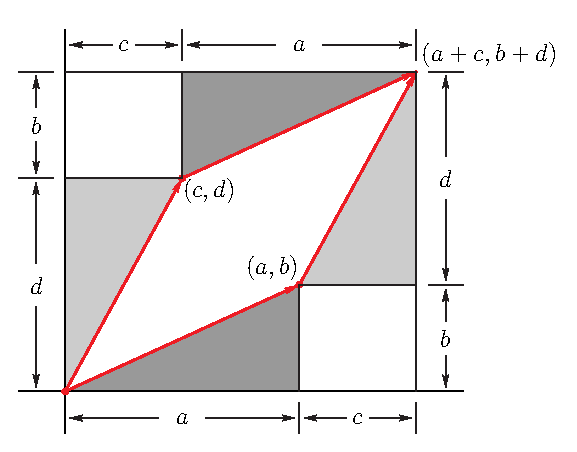
\includegraphics{area3}
      \end{center}
      \end{efig}
        }%
Any parallelogram can be constructed like this if you pick the common point
and two vectors appropriately. Let's compute the area of the parallelogram.
The area of the large rectangle with vertices $(0,0),\ (0, b+d),\ (a+c,0)$
and $(a+c,b+d)$ is $(a+c)(b+d)$. The parallelogram we want can be extracted
from the large rectangle by deleting the two small rectangles (each of
area $bc$), and the two lightly shaded triangles (each of area $\half cd$),
and the two darkly shaded triangles (each of area $\half ab$). So the desired
\begin{align*}
{\rm area} = (a+c)(b+d) - (2\times bc) -\big(2\times \half cd\big)
 -\big(2\times\half ab\big)
=ad-bc
\end{align*}
In the above figure, we have implicitly assumed that $a,\ b,\ c,\ d\ge 0$
and $d/c\ge b/a$. In words, we have assumed that both vectors 
$\llt a,b\rgt ,\ \llt c,d\rgt $ lie in the first quadrant and that 
$\llt c,d\rgt $ lies above $\llt a,b\rgt $.
By simply interchanging $a\leftrightarrow c$ and $b\leftrightarrow d$
in the picture and throughout the argument, we see that when 
$a,\ b,\ c,\ d\ge 0$ and $b/a\ge d/c$, so that the vector $\llt c,d\rgt $ 
lies below $\llt a,b\rgt $, the area of the parallelogram is $bc-ad$. 
In fact, all cases are covered by the formula
\begin{impeqn}\label{eq pgram area}
\begin{align*}
\text{area of parallelogram with sides $\llt a,b\rgt $ and $\llt c,d\rgt =|ad-bc|$}
\end{align*}
\end{impeqn}

Given two vectors $\llt a,b\rgt $ and $\llt c,d\rgt $, the expression 
$ad-bc$ is generally written
\begin{align*}
\det\left[\begin{matrix}a&b\\ c&d\end{matrix}\right]=ad-bc
\end{align*}
and is called the \emph{determinant} of the matrix\footnote{The topics of
matrices and determinants appear prominently in linear algebra courses. We
are only going to use them as notation, and we will explicitly explain
that notation. A linear algebra course is \emph{not} a prerequisite 
for this text.} 
\begin{align*}
\left[\begin{matrix}a&b\\ c&d\end{matrix}\right]
\end{align*} 
with rows $\llt a,b\rgt $ and $\llt c,d\rgt $. The determinant
of a $2\times 2$ matrix is the product of the diagonal entries 
minus the product of the off-diagonal entries. 


There is a similar formula in three dimensions. Any three vectors 
$\va=\llt a_1,a_2,a_3\rgt ,\ \vb=\llt b_1,b_2,b_3\rgt $ and 
$\vc=\llt c_1,c_2,c_3\rgt $ in three dimensions
\vadjust{
      \begin{efig} 
      \begin{center}
      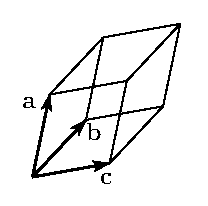
\includegraphics{piped}
      \end{center}
      \end{efig}
        }%
determine a parallelepiped 
(three dimensional parallelogram). Its volume is given by the formula
\begin{impeqn}\label{eq piped volume}
\begin{align*}
\text{volume of parallelepiped with edges $\va,\ \vb,\ \vc\ 
=\ \left|
\det\left[\begin{matrix}a_1&a_2&a_3\\ b_1&b_2&b_3\\ c_1&c_2&c_3\end{matrix}\right]
\right|$}
\end{align*}
\end{impeqn}
The determinant of a $3\times 3$ matrix can be defined in terms
of some $2\times 2$ determinants by
%      \begin{wfig} 
      \begin{center}
      \includegraphics{det2}%\qquad\null
      \end{center}
%      \end{wfig}
This formula is called ``expansion along the top row''. There
is one term in the formula for each entry in the top row of the $3\times 3$
matrix. The term is
a sign times the entry itself times the determinant of the $2\times 2$ matrix
gotten by deleting the row and column that contains the entry. The sign
alternates, starting with a $+$. 

We shall not prove this formula completely. It gets a little tedious.
But, there is one case in which we can easily verify that the volume of the 
parallelepiped is really given by the absolute value of the
claimed determinant. If the vectors $\vb$ and $\vc$ happen to lie
in the $xy$ plane, so that $b_3=c_3=0$, then 
\begin{align*}
\det\left[\begin{matrix}a_1&a_2&a_3\\ b_1&b_2&0\\ c_1&c_2&0\end{matrix}\right]
&=a_1(b_20-0c_2) -a_2(b_10-0c_1) +a_3(b_1c_2-b_2c_1)\\
&=a_3(b_1c_2-b_2c_1)
\end{align*}
The first factor, $a_3$, is the $z$-coordinate of the one vector not contained in the $xy$-plane. It 
is (up to a sign) the height of the parallelepiped. The second factor is,
up to a sign, the area of the parallelogram determined by $\vb$
and $\vc$. This parallelogram forms the base of the parallelepiped. 
The product is indeed, up to a sign, the volume of the parallelepiped.
That the formula is true in general is a consequence of the fact (that
we will not prove) that the value of a determinant does not change when
one rotates the coordinate system and that one can always rotate
our coordinate axes around so that $\vb$ and $\vc$ both lie in the
$xy$-plane. 


%%%%%%%%%%%%%%%%%%%%%%%%%%%%%%%%%%%%%%%%%%%%%%%%%%%%%%%
\subsection{The Cross Product}
%%%%%%%%%%%%%%%%%%%%%%%%%%%%%%%%%%%%%%%%%%%%%%%%%%%%%%%
We have already seen two different products involving vectors ---
the multiplication of a vector by a scalar 
and the dot product of two vectors. The dot product of two vectors
yields a scalar. We now introduce another product 
of two vectors, called the \emph{cross product}. The cross product of
two vectors will give a vector. There are applications which have two 
vectors as inputs and produce one vector as an output, and which are related
to the cross product. Here is a very brief mention of two such applications. 
We will look at them in much more detail later. 
\begin{itemize}
\item 
Consider a parallelogram in three dimensions.
A parallelogram is naturally determined by the two vectors that define 
its sides.
One measure of the size of a parallelogram is its area. 
One way to specify the orientation of the parallelogram is to give a vector
that is perpendicular to it. 
A very compact way to encode both the area and the orientation of
the parallelogram is to give a vector whose direction is perpendicular 
to the plane in which it lies and whose magnitude is its area.
We shall see that such a vector can be easily constructed by taking the cross product (definition coming shortly) of the two vectors that give
the sides of the parallelogram.

      \begin{nfig} 
      \begin{center}
      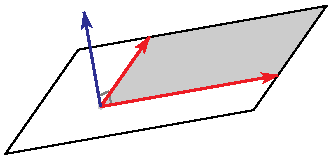
\includegraphics{pgramCross.pdf}
      \end{center}
      \end{nfig}

\item 
Imagine a rigid body which is rotating at a rate $\Omega$ radians per 
second about an axis whose direction is given by the unit vector $\hat\va$. 
Let $P$ be any point on the body. We shall see, in the (optional)
\S\ref{sec rot motion}, that the velocity, $\vv$, of the point $P$ 
is the cross product 
(again, definition coming shortly) of the vector $\Om\hat\va$ with the vector
$\vr$ from any point on the axis of rotation to $P$.
      \begin{nfig} 
      \begin{center}
      \includegraphics{rigidBB}
      \end{center}
      \end{nfig}
\end{itemize}

\noindent
Finally, here is the definition of the cross product.

\begin{defn}[Cross Product]\label{def:crossProd}
The cross product of the vectors $\va=\llt a_1,a_2,a_3\rgt$ and 
$\vb=\llt b_1,b_2,b_3\rgt$ is denoted $\va\times\vb$ 
and is defined by
\begin{align*}
\va\times\vb = \llt a_2b_3-a_3b_2\,,\, a_3b_1-a_1b_3\,,\, a_1b_2-a_2b_1\rgt 
\end{align*}
\end{defn}

Note that each component has the form $a_ib_j-a_jb_i$. The index $i$ of
the first $a$ in component number $k$ of $\va\times\vb$
is just after $k$ in the list $1,2,3,1,2,3,1,2,3,\cdots$. 
The index $j$ of the first $b$ is just before $k$ in the list. 
\begin{align*}
(\va\times\vb)_k
=a_{{\rm just\  after\  }k}\ b_{{\rm just\  before\  }k}
-a_{{\rm just\  before\  }k}\ b_{{\rm just\  after\  }k}
\end{align*}
For example, for component number $k=3$,
\begin{align*}
\left.{\text{``just after 3'' is 1}}\atop{\text{``just before 3'' is 2}}\right\}
\implies (\va\times\vb)_3= a_1b_2-a_2b_1
\end{align*}


There is a much better way to remember this definition. Recall that
a $2\times 2$ matrix is an array of numbers having two rows and two columns
and that the determinant of a $2\times 2$ matrix is  defined by
\begin{align*}
\det \left[\begin{matrix}a& b\\ c&d\end{matrix}\right]=ad-bc
\end{align*}
It is the product of the entries on the diagonal minus the product
of the entries not on the diagonal. 

A $3\times 3$ matrix is an array of
numbers having three rows and three columns.
\begin{align*}
 \left[\begin{matrix}i& j &k\\ a_1&a_2&a_3\\ b_1&b_2&b_3\end{matrix}\right]
\end{align*}
You will shortly see why the entries in the top row have been given the
rather peculiar names $i$, $j$ and $k$. The determinant of a $3\times 3$ 
matrix can be defined in terms of some $2\times 2$ determinants by
      \begin{center}
      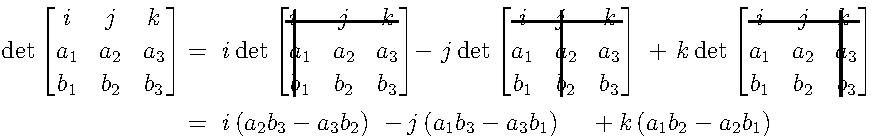
\includegraphics{det.pdf}
      \end{center}
This formula is called ``expansion of the determinant along the top row''. 
There is one term in the formula for each entry in the top row. The term is
a sign times the entry itself times the determinant of the $2\times 2$ matrix
gotten by deleting the row and column that contains the entry. The sign
alternates, starting with a $+$. If we now replace $i$ by $\hi$, $j$ by $\hj$ 
and $k$ by $\hk$, we get exactly the formula for $\va\times \vb$
of Definition \ref{def:crossProd}. That is the reason for the peculiar 
choice of names for the matrix entries. So
\begin{align*}
\va\times\vb
&=\det\left[\begin{matrix}\hi& \hj &\hk\\ 
                            a_1&a_2&a_3\\ 
                            b_1&b_2&b_3\end{matrix}\right] \\
&=\hi\big(a_2b_3-a_3b_2) -\hj(a_1b_3-a_3b_1) +\hk(a_1b_2-a_2b_1)
\end{align*}
is a mnemonic device for remembering the definition of $\va\times\vb$.
It is also good from the point of view of 
evaluating $\va\times\vb$.

\begin{eg}\label{eg:GEOcrossijji}
In this example, we'll use the mnemonic device to compute two very simple cross
products. First
      \begin{center}
      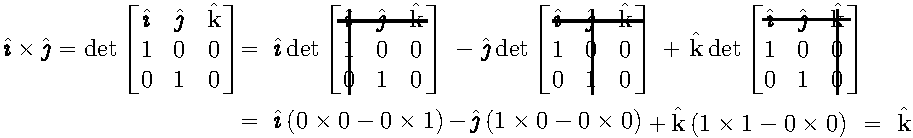
\includegraphics{detij.pdf}
      \end{center}
Second
      \begin{center}
      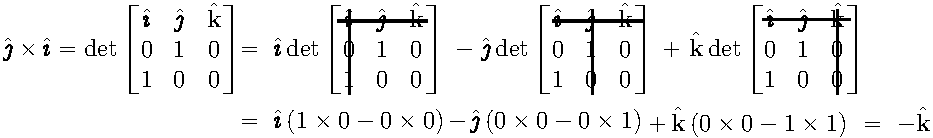
\includegraphics{detji.pdf}
      \end{center}
Note that, unlike most (or maybe even all) products that you have seen before, $\hi\times\hj$ is \emph{not} the same as $\hj\times\hi$!
\end{eg}

Our first properties of the cross product 
lead up to a more intuitive geometric definition of $\va\times\vb$, which is better for interpreting $\va\times\vb$. 
 These properties of the cross product, which state that  $\va\times\vb$
is a vector and then determine its direction and length, are as follows.
We will collect these properties, and a few others, into a theorem shortly.
\begin{enumerate}[(1)]
\setcounter{enumi}{-1}
\item $\va,\vb\text{ are vectors in three dimensions and }
\va\times\vb\text{ is a vector in three dimensions}$.

\item $\va\times\vb$ is perpendicular to both  $\va$ and $\vb$.

\textit{Proof}: To check that $\va$ and $\va\times \vb$ are perpendicular, 
one just has to check that the dot product $\va\cdot(\va\times \vb)=0$.
The six terms in 
\begin{equation*}
\va\cdot(\va\times \vb)=
a_1(a_2b_3-a_3b_2)+a_2(a_3b_1-a_1b_3)+a_3(a_1b_2-a_2b_1)
\end{equation*} 
cancel pairwise. The computation showing that $\vb\cdot(\va\times \vb)=0$ 
is similar.

\bigskip
\item $|\va\times\vb|=|\va|\,|\vb|\sin\theta
\text{ where $0\le\theta\le\pi$ is the angle between $\va$ and $\vb$}$

$\phantom{|\va\times\vb|}=\text{the area of the parallelogram
with sides $\va$ and $\vb$}\qquad\qquad\quad
\smash{\raisebox{-0.2\height}{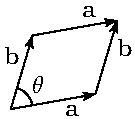
\includegraphics{area.pdf}}}$

\textit{Proof}: 
%This follows from 
%$|\va\times\vb|^2
%=|\va|^2|\vb|^2-(\va\cdot\vb)^2
%=|\va|^2|\vb|^2(1-\cos^2\theta)$ which in turn is gotten by comparing
The formula $|\va\times\vb|=|\va|\,|\vb|\sin\theta$ is gotten by comparing
\begin{align*}
|\va\times\vb|^2
&=\big(\va\times\vb\big)\cdot\big(\va\times\vb\big) \\
&=(a_2b_3-a_3b_2)^2+(a_3b_1-a_1b_3)^2+ (a_1b_2-a_2b_1)^2\\
&=a_2^2b_3^2-2a_2b_3a_3b_2+a_3^2b_2^2
+a_3^2b_1^2-2a_3b_1a_1b_3+a_1^2b_3^2\\&\hskip0.5in
+a_1^2b_2^2-2a_1b_2a_2b_1+a_2^2b_1^2\\
\intertext{and}
|\va|^2\,|\vb|^2\sin^2\theta
&=|\va|^2|\vb|^2(1-\cos^2\theta)\\
&=|\va|^2|\vb|^2-(\va\cdot\vb)^2 \\
&=\big(a_1^2+a_2^2+a_3^2\big)\big(b_1^2+b_2^2+b_3^2\big)
-\big(a_1b_1+a_2b_2+a_3b_3\big)^2\\
&=a_1^2b_2^2+a_1^2b_3^2+a_2^2b_1^2+a_2^2b_3^2+a_3^2b_1^2+a_3^2b_2^2\\
&\hskip0.5in
 -\big(2a_1b_1a_2b_2+2a_1b_1a_3b_3+2a_2b_2a_3b_3\big)\\
\end{align*}
To see that $|\va|\,|\vb|\sin\theta$ is the area of the parallelogram
with sides $\va$ and $\vb$, just recall that the area of any parallelogram
is given by the length of its base times its height. Think of $\va$ as the
base of the parallelogram. Then $|\va|$ is the length of the base
and $|\vb|\sin\theta$ is the height.
      \begin{efig} 
      \begin{center}
      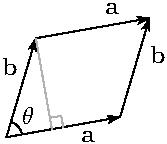
\includegraphics{areaB.pdf}
      \end{center}
      \end{efig}


\end{enumerate}

\noindent
These properties almost determine $\va\times\vb$. Property 1 forces
the vector $\va\times\vb$ to lie on the line perpendicular to the
plane containing $\va$ and $\vb$. There are precisely two vectors
on this line that have the length given by property 2. In the left hand
figure of
      \begin{efig} 
      \begin{center}
      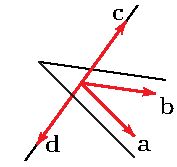
\includegraphics{crossLL.pdf}\qquad\quad
      \raisebox{-0.05\height}{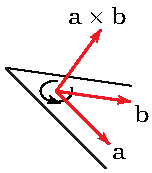
\includegraphics{crossRR.pdf}}\qquad\quad
%    \raisebox{0.05\height}{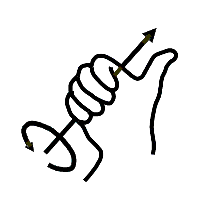
\includegraphics[scale=0.8]{Right-hand_rule.pdf}}
    \raisebox{0.2\height}{
\includegraphics[scale=0.4]{RHR.pdf}}
      \end{center}
      \end{efig}
the two vectors are labeled $\vc$ and $\vd$. Which of these two
candidates is correct is determined by the right hand rule\footnote{
That the cross product uses the right hand rule, rather than the left hand rule, is an example of the tyranny of the masses --- only roughly 10\% 
of humans are left-handed. }, which says
that if you form your right hand into a fist with your fingers curling from 
$\va$ to $\vb$, then when you stick your thumb straight out from
the fist, it points in the direction of $\va\times\vb$. This is
illustrated in the figure on the right 
above
\footnote{This figure is a variant of 
https:/\hskip-1pt/commons.wikimedia.org/wiki/File:Right\_hand\_rule\_simple.png
}.
The important special cases

\begin{enumerate}[(1)]
\setcounter{enumi}{2}
\item $\hi\times\hj=\phantom{-}\hk,\ \ \ \hj\times\hk=\phantom{-}\hi,\ \ \  \hk\times\hi=\phantom{-}\hj$ \\
      $\hj\times\hi=-\hk,\ \ \ \hk\times\hj=-\hi,\ \ \ \hi\times\hk=-\hj$

all follow directly from the definition of the cross product (see, for example,
Example \ref{eg:GEOcrossijji}) and all 
obey the right hand rule.  Combining properties 1, 2 and the right hand 
rule give the geometric definition of $\va\times\vb$. To remember
these three special cases, just remember this figure.
      \begin{efig} 
      \begin{center}
      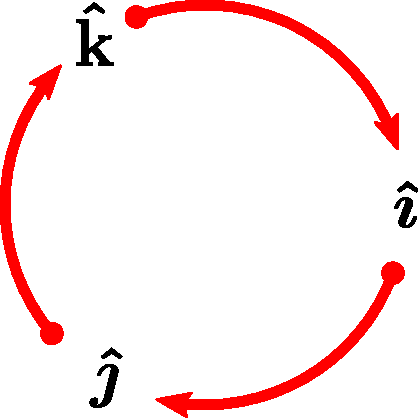
\includegraphics[scale=0.3]{cp_circle.pdf}
      \end{center}
      \end{efig}
The product of any two standard basis vectors, taken in the order of 
the arrows in the figure, is the third standard basis vector.
Going against the arrows introduces a minus sign.


\item $\va\times\vb=|\va|\,|\vb|\sin\theta\ \hn
\text{ where $\theta$ is the angle between $\va$ and $\vb$, }
|\hn|=1,\ \hn\perp\va,\vb$
  and $(\va,\vb,\hn)$ obey the right hand rule.

\textit{Outline of Proof}: We have already seen that the right hand side
has the correct length and, except possibly for a sign, direction.
To check that the right hand rule holds in
general, rotate your coordinate system around\footnote{Note that as you 
translate or rotate the coordinate system, the right hand rule is preserved. 
If $(\va,\vb,\hn)$ obey the right hand rule so do their rotated and 
translated versions.} 
so that $\va$ points along
the positive $x$ axis and $\vb$ lies in the $xy$-plane with positive
$y$ component. That is $\va=\alpha\hi$ and $\vb=\beta\hi+\gamma
\hj$ with $\alpha,\gamma\ge 0$. Then 
$\va\times\vb=\alpha\hi\times(\beta\hi+\gamma\hj)
=\alpha\beta\,\hi\times\hi+\alpha\gamma\,\hi\times\hj$. The
first term vanishes by property 2, because the angle $\theta$ between $\hi$
and $\hi$ is zero. So, by property 3, 
$\va\times\vb= \alpha\gamma\hk$ points
along the positive $z$ axis, which is consistent with the right hand rule.

\end{enumerate}

\noindent  The analog of property 7 of the dot product (which says that
$\va\cdot\vb$ is zero if and only if  $\va=\vZero$ or $\vb=\vZero$ or  $\va\perp\vb$) follows
immediately from property 2.

\begin{enumerate}[(1)]
\setcounter{enumi}{4}

\item $\va\times\vb=\vZero\iff \va=\vZero \text{ or }\vb=\vZero 
\text{ or }\va\parallel\vb$

\end{enumerate}

\noindent
The remaining properties are all tools for
helping do computations with cross products.
Here is a theorem which summarizes the properties of the cross product.
We have already seen the first five. The other properties are all tools 
for helping do computations with cross products.

\begin{theorem}[Properties of the Cross Product]\label{thm:crossPppties}
\begin{enumerate}[(1)]
\setcounter{enumi}{-1}

\item $\va,\vb\text{ are vectors in three dimensions and }
\va\times\vb\text{ is a vector in three dimensions}$.

\item $\va\times\vb$ is perpendicular to both  $\va$ and $\vb$.

\bigskip
\item $|\va\times\vb|=|\va|\,|\vb|\sin\theta
\text{ where $\theta$ is the angle between $\va$ and $\vb$}$

$\phantom{|\va\times\vb|}=\text{the area of the parallelogram
with sides $\va$ and $\vb$}\qquad
\smash{\raisebox{-0.1\height}{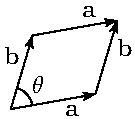
\includegraphics{area.pdf}}}$

\item $\hi\times\hj=\hk,\ \hj\times\hk=\hi,\ \hk\times\hi=\hj$


\item $\va\times\vb=|\va|\,|\vb|\sin\theta\ \vn
\text{ where $\theta$ is the angle between $\va$ and $\vb$, }
|\vn|=1,\\ \vn\perp\va,\vb$
  and $(\va,\vb,\vn)$ obey the right hand rule.

\item $\va\times\vb=\vZero\iff \va=\vZero \text{ or }\vb=\vZero 
\text{ or }\va\parallel\vb$


\end{enumerate}
\end{theorem}

\addtocounter{theorem}{-1}
\begin{theorem}[continued]
\begin{enumerate}[(1)]
\setcounter{enumi}{5}

\item $\va\times \vb=-\vb\times\va$

\item $(s\va)\times \vb=\va\times(s\vb)=s(\va\times \vb)$ for any scalar
(i.e. number) $s$.

\item $\va\times(\vb+\vc)=\va\times\vb+\va\times \vc$

\item $\va\cdot(\vb\times\vc)=(\va\times\vb)\cdot\vc$

\item $\va\times(\vb\times\vc)=(\vc\cdot\va)\vb -(\vb\cdot\va)\vc$
\end{enumerate}

\end{theorem}
\begin{proof}
We have already seen the proofs up to number 5. Numbers 6, 7 and 8 
follow immediately from the definition, using a little algebra. To prove 
numbers 9 and 10 we just write out the definitions of the left hand sides 
and the right hand sides and observe that they are equal.

\medskip
\noindent (9)\ \ \ The left hand side is
\begin{align*}
\va\cdot(\vb\times\vc)
&=\llt a_1,a_2,a_3\rgt\cdot
      \llt b_2c_3-b_3c_2\,,\, b_3c_1-b_1c_3\,,\, b_1c_2-b_2c_1\rgt\\
&=a_1b_2c_3 - a_1b_3c_2 + a_2b_3c_1 - a_2b_1c_3 + a_3b_1c_2 - a_3b_2c_1
\end{align*}
The right hand side is
\begin{align*}
(\va\times\vb)\cdot\vc
&=\llt a_2b_3-a_3b_2\,,\, a_3b_1-a_1b_3\,,\, a_1b_2-a_2b_1\rgt\cdot
       \llt c_1,c_2,c_3\rgt \\
&=a_2b_3c_1 - a_3b_2c_1 + a_3b_1c_2 - a_1b_3c_2 + a_1b_2c_3 - a_2b_1c_3
\end{align*}
The left and right hand sides are the same.

\medskip
\noindent (10)\ \ \ Since
$$
\vb\times\vc
\ =\ (b_2c_3-b_3c_2)\,\hi-(b_1c_3-b_3c_1)\,\hj
    +(b_1c_2-b_2c_1)\,\hk
$$
The left hand side is
\begin{align*}
\va\times(\vb\times\vc)
\ =\ &\det\left[\begin{matrix} \hi & \hj & \hk \\
                     a_1&a_2&a_3\\
                 b_2c_3-b_3c_2&-b_1c_3+b_3c_1&b_1c_2-b_2c_1
             \end{matrix}\right]\\[0.05in]
\ =\ &\phantom{-}\hi\,[a_2(b_1c_2-b_2c_1)-a_3(-b_1c_3+b_3c_1)]\\
     & {-}\hj\,[a_1(b_1c_2-b_2c_1)-a_3(b_2c_3-b_3c_2)]\\
     & {+}\hk\,[a_1(-b_1c_3+b_3c_1)-a_2(b_2c_3-b_3c_2)]
\end{align*}
The right hand side is
\begin{align*}
(\va\cdot\vc)\vb-(\va\cdot\vb)\vc
&=(a_1c_1+a_2c_2+a_3c_3)(b_1\hi+b_2\hj+b_3\hk) \\
     &\hskip1in -(a_1b_1+a_2b_2+a_3b_3)(c_1\hi+c_2\hj+c_3\hk)\\
&=\phantom{-}
\hi[a_1b_1c_1+a_2b_1c_2+a_3b_1c_3-a_1b_1c_1-a_2b_2c_1-a_3b_3c_1] \\
&\phantom{=}+\hj[a_1b_2c_1+a_2b_2c_2+a_3b_2c_3-a_1b_1c_2-a_2b_2c_2-a_3b_3c_2] \\
&\phantom{=}+\hk[a_1b_3c_1+a_2b_3c_2+a_3b_3c_3-a_1b_1c_3-a_2b_2c_3-a_3b_3c_3]
\\[0.05in]
&=\phantom{-} \hi[a_2b_1c_2+a_3b_1c_3-a_2b_2c_1-a_3b_3c_1] \\
 &\phantom{=} +\hj[a_1b_2c_1+a_3b_2c_3-a_1b_1c_2-a_3b_3c_2]\\
 &\phantom{=} +\hk[a_1b_3c_1+a_2b_3c_2-a_1b_1c_3-a_2b_2c_3]
\end{align*}
The left and right hand sides are the same. Oof! This is a little tedious
to do by hand. But any computer algebra system will do it for you in a 
flash.
\end{proof}


\begin{warning}\label{warning:GEOMcross} 
Take particular care with properties 6 and 10. They are 
counterintuitive and are a frequent source of errors. In particular, 
for general vectors $\va$, $\vb$, $\vc$, the cross product is neither
commutative nor associative, meaning that
\begin{align*}
\va\times\vb&\ne\vb\times\va\\
\va\times(\vb\times\vc)&\ne (\va\times\vb)\times\vc
\end{align*} 
For example
\begin{align*}
\hi\times(\hi\times\hj)
&=\hi\times\hk=-\hk\times\hi =-\hj\\
(\hi\times \hi)\times\hj&= \vZero \times\hj=\vZero\\
\end{align*} 
\end{warning}

\begin{eg}\label{eg:GEOcross}
As an illustration of the properties of the dot and cross product, we now
derive the formula for the volume of the parallelepiped with edges 
$\va=\llt a_1,a_2,a_3\rgt $, $\vb = \llt b_1,b_2,b_3\rgt $, 
$\vc = \llt c_1,c_2,c_3\rgt $ that was mentioned in 
\S\ref{sec:GEOparallelogram}.
\vadjust{
      \begin{efig} 
      \begin{center}
      \includegraphics{pipedVolume.pdf}
      \end{center}
      \end{efig}
        }%
The volume of the parallelepiped is the area of its base times its 
height\footnote{This is a simple integral calculus exercise.}.
The base is the parallelogram with sides $\vb$ and
$\vc$. Its area is the length of its base, which is $|\vb|$,
times its height, which is $|\vc|\,\sin\theta$. (Drop a 
perpendicular from the head of $\vc$ to the line containing $\vb$). 
Here $\theta$ is the angle between $\vb$ and $\vc$. So the area of the 
base is $|\vb|\,|\vc|\,\sin\theta= |\vb\times\vc|$, by 
property 2 of the cross product. To get the height of the parallelepiped, 
we drop a perpendicular from the head of $\va$ to the line that passes 
through the tail of $\va$ and is perpendicular to the base of the parallelepiped. In other words, from
the head of $\va$ to the line that contains both the head and the tail
of $\vb\times\vc$. So the height of the parallelepiped is
$|\va|\,|\cos\varphi|$.  (The absolute values have been included because 
if the angle between $\vb\times\vc$ and $\va$ happens to be greater
than $90^\circ$, the $\cos\varphi$ produced by taking the dot product of 
$\va$ and  $(\vb\times\vc$) will be negative.) All together
\begin{align*}
\text{volume of parallelepiped}
&=(\text{area of base})\,(\text{height})\\
&=|\vb\times\vc|\ |\va|\ |\cos\varphi|\\
&=\big|\va\cdot(\vb\times\vc)\big|\\
&=\left|a_1 (\vb\times\vc)_1 +a_2 (\vb\times\vc)_2 
               +a_3 (\vb\times\vc)_3\right|\\
&=\left|a_1\det\left[\begin{matrix}b_2&b_3\\ c_2&c_3\end{matrix}\right] 
        -a_2 \det\left[\begin{matrix}b_1&b_3\\ c_1&c_3\end{matrix}\right] 
               +a_3\det\left[\begin{matrix}b_1&b_2\\ c_1&c_2\end{matrix}\right]\right|\\
&=\left|\det\left[\begin{matrix}a_1&a_2&a_3\\
                          b_1&b_2&b_3\\
                          c_1&c_2&c_3\end{matrix}\right]\right|
\end{align*}

\end{eg}


\begin{eg}\label{eg:GEOcrossConcrete}
As a concrete example of the computation of the volume of a parallelepiped,
we consider the parallelepiped with edges
\begin{align*}
\va &= \llt 0,1,2\rgt \\
\vb &= \llt 1,1,0\rgt \\
\vc &= \llt 0,1,0\rgt
\end{align*}
Here is a sketch.
\vadjust{
      \begin{efig} 
      \begin{center}
      \includegraphics{pipedVolumeEg.pdf}
      \end{center}
      \end{efig}
        }%
The base of the parallelepiped is the parallelogram with sides $\vb$ and $\vc$.
It is the shaded parallelogram in the sketch above. As
\begin{align*}
\vb\times\vc
&=\det\left[\begin{matrix}\hi& \hj &\hk\\ 
                            1&1&0\\ 
                            0&1&0\end{matrix}\right] \\
&=\hi\det\left[\begin{matrix} 1&0\\ 
                              1&0\end{matrix}\right]
  -\hj\det\left[\begin{matrix}1&0\\ 
                              0&0\end{matrix}\right] 
   +\hk\det\left[\begin{matrix} 1&1\\ 
                                0&1\end{matrix}\right] \\
&=\hi\big(1\times 0-0\times 1) -\hj(1\times 0-0\times 0) 
                  +\hk(1\times 1-1\times 0) \\
&=\hk
\end{align*}
We should not be surprised that $\vb\times\vc$ has direction $\hk$.
\begin{itemize}\itemsep1pt \parskip0pt \parsep0pt
\item[$\circ$]
$\vb\times\vc$ has to be perpendicular to both $\vb$ and $\vc$ and 
\item[$\circ$]
both $\vb$ and $\vc$ lie in the $xy$-plane, 
\item[$\circ$]
so that $\vb\times\vc$ has to the parallel to the $z$-axis.
\end{itemize}
The area of the base, i.e. of the shaded parallelogram in the figure above,
is
\begin{equation*}
|\vb\times\vc| = |\hk| =1
\end{equation*}
and the volume of the parallelepiped is
\begin{equation*}
|\va\cdot (\vb\times\vc)|
= |\llt 0,1,2\rgt\cdot\llt 0,0,1\rgt|=2
\end{equation*}

\end{eg}

%%%%%%%%%%%%%%%%%%%%%%%%%%%%%%%%%%%%%%%%%%%%%%%%%%%%%%%%%%%%%%%%%%%
\subsection{(Optional) Some Vector Identities}
\label{sec vector identities}

Here are a few identities involving dot and cross products.
\begin{lemma}\label{lem:tripProd}
\begin{enumerate}[(a)]
\item\ \ \ 
$\va\cdot(\vb\times\vc)=(\va\times\vb)\cdot\vc$
\item\ \ \ 
$\va\times(\vb\times\vc)=(\vc\cdot\va)\vb-(\vb\cdot\va)\vc$
\item\ \ \ 
           $\va\times(\vb\times\vc) + 
            \vb\times(\vc\times\va) +
            \vc\times(\va\times\vb) =\vZero$
\end{enumerate}
\end{lemma}
\begin{proof} (a)
Here are two proofs.
For the first, just write out both sides
\begin{align*}
\va\cdot(\vb\times\vc)
&=(a_1,a_2,a_3)\cdot(b_2c_3-b_3c_2\,,\,b_3c_1-b_1c_3\,,\,b_1c_2-b_2c_1)\\
&=a_1b_2c_3-a_1b_3c_2+a_2b_3c_1-a_2b_1c_3+a_3b_1c_2-a_3b_2c_1\\
(\va\times\vb)\cdot\vc
&=(a_2b_3-a_3b_2\,,\,a_3b_1-a_1b_3\,,\,a_1b_2-a_2b_1)\cdot(c_1,c_2,c_3)\\
&=a_2b_3c_1-a_3b_2c_1+a_3b_1c_2-a_1b_3c_2+a_1b_2c_3-a_2b_1c_3
\end{align*}
and observe that they are the same.

\medskip
For the second proof,
we again write out both sides, but this time we express them
in terms of determinants.
\begin{align*}
\va\cdot\vb\times\vc
&=(a_1,a_2,a_3)\cdot\det\left[\begin{matrix}\hi&\hj&\hk\\
                                       b_1&b_2&b_3\\
                                       c_1&c_2&c_3\end{matrix}\right]\\
&=a_1\det\left[\begin{matrix}
                                       b_2&b_3\\
                                       c_2&c_3\end{matrix}\right]
                             -a_2\det\left[\begin{matrix}
                                       b_1&b_3\\
                                       c_1&c_3\end{matrix}\right]
                             +a_3\det\left[\begin{matrix}
                                       b_1&b_2\\
                                       c_1&c_2\end{matrix}\right]\\
&=\det\left[\begin{matrix}a_1&a_2&a_3\\
                                       b_1&b_2&b_3\\
                                       c_1&c_2&c_3\end{matrix}\right]\\[0.1in]
\va\times\vb\cdot\vc
&=\det\left[\begin{matrix}\hi&\hj&\hk\\
                     a_1&a_2&a_3\\
                     b_1&b_2&b_3\end{matrix}\right]\cdot(c_1,c_2,c_3)\\
&=c_1\det\left[\begin{matrix}
                                       a_2&a_3\\
                                       b_2&b_3\end{matrix}\right]
                             -c_2\det\left[\begin{matrix}
                                       a_1&a_3\\
                                       b_1&b_3\end{matrix}\right]
                             +c_3\det\left[\begin{matrix}
                                       a_1&a_2\\
                                       b_1&b_2\end{matrix}\right]\\
&=\det\left[\begin{matrix}c_1&c_2&c_3\cr a_1&a_2&a_3\\
                                       b_1&b_2&b_3\\
                                       \end{matrix}\right]
\end{align*}
Exchanging two rows in a determinant changes the sign of the determinant.
Moving the top row of a $3\times 3$ determinant to the bottom row requires
two exchanges of rows.
So the two $3\times 3$ determinants are equal.

\noindent (b)
The proof is not exceptionally difficult --- just write out both sides and grind.
Substituting in
\begin{equation*}
\vb\times\vc
\ =\ (b_2c_3-b_3c_2)\hi-(b_1c_3-b_3c_1)\hj + (b_1c_2-b_2c_1)\hk
\end{equation*}
gives, for the left hand side,
\begin{align*}
\va\times(\vb\times\vc)
=\phantom{-}&\!\!\!\det\left[\begin{matrix}\hi&\hj &\hk\\
                     a_1&a_2&a_3\\
                     b_2c_3-b_3c_2&-b_1c_3+b_3c_1&b_1c_2-b_2c_1
                     \end{matrix}\right]\\[0.1in]
=\phantom{-}&\hi\big[a_2(b_1c_2-b_2c_1)-a_3(-b_1c_3+b_3c_1)\big]\\
-&\hj\big[a_1(b_1c_2-b_2c_1)-a_3(b_2c_3-b_3c_2)\big]\\
+&\hk\big[a_1(-b_1c_3+b_3c_1)-a_2(b_2c_3-b_3c_2)\big]
\end{align*}
On the other hand, the right hand side
\begin{align*}
(\va\cdot\vc)\vb-(\va\cdot\vb)\vc
\ =\ &(a_1c_1+a_2c_2+a_3c_3)(b_1\hi+b_2\hj+b_3\hk)
-(a_1b_1+a_2b_2+a_3b_3)(c_1\hi+c_2\hj+c_3\hk)\cr
=\ &
\hi\ \big[\textcolor{blue}{a_1b_1c_1}
         +a_2b_1c_2+a_3b_1c_3-
         \textcolor{blue}{a_1b_1c_1}
         -a_2b_2c_1-a_3b_3c_1\big]
\\
{+}&\hj\ \big[a_1b_2c_1
      +\textcolor{blue}{a_2b_2c_2}
      +a_3b_2c_3-a_1b_1c_2
      -\textcolor{blue}{a_2b_2c_2}
      -a_3b_3c_2\big]
\cr
{+}&\hk\ \big[a_1b_3c_1+a_2b_3c_2
          +\textcolor{blue}{a_3b_3c_3}
          -a_1b_1c_3-a_2b_2c_3
          -\textcolor{blue}{a_3b_3c_3}\big]
\\
{=}\ &
\hi\ [a_2b_1c_2+a_3b_1c_3-a_2b_2c_1-a_3b_3c_1]
\cr
{+}&\hj\ [a_1b_2c_1+a_3b_2c_3-a_1b_1c_2-a_3b_3c_2]
\cr
{+}&\hk\ [a_1b_3c_1+a_2b_3c_2-a_1b_1c_3-a_2b_2c_3]
\end{align*}
The last formula that we had for the left hand side is the same as the last formula we had for the right hand side.

\noindent (c)
We just apply part (b) three times
\begin{align*}
          &\va\times(\vb\times\vc) + 
            \vb\times(\vc\times\va) +
            \vc\times(\va\times\vb)  \\
&\hskip0.5in= (\vc\cdot\va)\vb-(\vb\cdot\va)\vc
            + (\va\cdot\vb)\vc-(\vc\cdot\vb)\va
            + (\vb\cdot\vc)\va-(\va\cdot\vc)\vb \\
&\hskip0.5in=\vZero            
\end{align*}
\end{proof}



%%%%%%%%%%%%%%%%%%%%%%%%%%%%%%%%%%%%%%%%%%%%%%%%%%%%%%%%%%%%%%%%%%%
\subsection{(Optional) Application of Cross Products to Rotational Motion}
\label{sec rot motion}
%%%%%%%%%%%%%%%%%%%%%%%%%%%%%%%%%%%%%%%%%%%%%%%%%%%%%%%%%%%%%%%%%%%
In most computations involving rotational motion, the cross product shows
up in one form or another. This is one of the main applications of the cross
product. Consider, for example, a rigid body which is rotating 
 at a constant rate of $\Omega$ radians per second about an axis 
whose direction is given by the unit vector $\hat\va$. Let $P$ be any point
on the body. Let's figure out its velocity. Pick any point on the axis
of rotation and designate it as the origin of our coordinate system. Denote
by $\vr$ the vector from the origin to the point $P$. Let $\theta$ denote
the angle between $\hat\va$ and $\vr$. As time progresses the point $P$
sweeps out a circle of radius $R=|\vr\,|\sin\theta$.
      \begin{efig} 
      \begin{center}
      \includegraphics{rigid}
      \end{center}
      \end{efig}
In one second $P$ travels along an arc that subtends an angle of 
$\Omega$ radians, which is the fraction $\tfrac{\Omega}{2\pi}$ 
of a full circle.  The length of this arc is
$\tfrac{\Omega}{2\pi}\times 2\pi R=\Omega R=\Omega|\vr\,|\sin\theta$ so $P$ travels the distance $\Omega|\vr\,|\sin\theta$
in one second and its speed, which is also the length of its velocity vector,
is $\Omega|\vr\,|\sin\theta$. 

Now we just need to figure out the direction
of the velocity vector. That is, the direction of motion of the point $P$.
Imagine that both $\hat\va$ and $\vr$ lie in the plane of a piece of paper, 
as in the figure above. Then $\vv$ points either straight into 
or straight out of the page and consequently is perpendicular
to both $\hat\va$ and $\vr$. To distinguish between the ``into the page''
and ``out of the page'' cases, let's impose the conventions that 
$\Omega>0$ and the axis of rotation $\hat\va$ is chosen to obey the right hand
 rule, meaning that if the thumb of
your right hand is pointing in the direction $\hat\va$, then your fingers
are pointing in the direction of motion of the rigid body.  Under these
conventions, the velocity vector $\vv$ obeys
\begin{itemize}
\item $|\vv|=\Omega|\vr||\hat\va|\sin\theta$
\item $\vv\perp\hat\va,\vr$
\item $(\hat\va,\vr,\vv)$ obey the right hand rule
\end{itemize}
That is, $\vv$ is exactly $\Omega\hat\va\times\vr$. It is conventional
to define the ``angular velocity'' of a rigid body to be vector
$\mathbf{\Omega}=\Omega\hat\va$. That is, the vector with length given 
by the rate of rotation and direction given by the axis of rotation 
of the rigid body. In particular, the bigger the rate of rotation, the longer
the angular velocity vector. In terms of this angular 
velocity vector, the velocity of the point $P$ is
\begin{align*}
\vv=\mathbf{\Omega}\times\vr
\end{align*}

%%%%%%%%%%%%%%%%%%%%%%%%%%%%%%%%%%%%%%%%%%%%%%%%%%%%%%%%%%%%%%%%%%%
\subsection{(Optional) Application of Cross Products to Rotating Reference Frames}\label{sec rot frame}
%%%%%%%%%%%%%%%%%%%%%%%%%%%%%%%%%%%%%%%%%%%%%%%%%%%%%%%%%%%%%%%%%%%

Imagine a moving particle that is being tracked by two observers.
\begin{enumerate}[(a)]
\item One observer is fixed (out in space) and measures the position of 
  the particle to be $\big(X(t), Y(t), Z(t)\big)$.
\item The other observer is tied to a merry-go-round (the Earth) and 
  measures the position of the particle to be $\big(x(t),y(t),z(t)\big)$.
\end{enumerate}
The merry-go-round is sketched in the figure on the left below. It
is rotating about the $Z$-axis at a (constant) rate of $\Omega$ radians per second.
The vector $\vOmega = \Omega \hk$, whose length is the rate of rotation and
whose direction is the axis of rotation, is called the angular velocity.
\vadjust{
      \begin{efig} 
      \begin{center}
      \includegraphics{merry.pdf}\qquad\qquad
      \includegraphics{merryB.pdf}
      \end{center}
      \end{efig}
        }%
The $x$- and $y$-axes of the moving observer are painted in red on
the merry-go-round. The figure on the right above shows a top view of the
merry-go-round. The $x$- and $y$-axes of the moving observer are again
red. The $X$- and $Y$-axes of the fixed observer are blue.  We are
assuming that at time $0$, the $x$-axis of the moving observer and 
the $X$-axis of the fixed observer coincide. As the merry-go-round
is rotating at $\Om$ radians per second, the angle between the $X$-axis
and $x$-axis after $t$ seconds is $\Omega t$.

As an example, suppose that the moving particle is tied to the tip of the
moving observer's unit $x$ vector. Then
\begin{align*}
x(t) & = 1 &  y(t) &= 0 & z(t) &= 0 \\
X(t) & = \cos(\Om t) &  Y(t) &=\sin(\Om t) & Z(t) &= 0 
\end{align*}
or, if we write $\vr(t) = \big(x(t), y(t), z(t)\big)$ and 
$\vR(t) = \big(X(t), Y(t), Z(t)\big)$, then
\begin{align*}
\vr(t) = (1\,,\,0\,,\,0) \qquad
\vR(t)= \big(\cos(\Om t)\,,\,\sin(\Om t)\,,\,0\Big)
\end{align*}

In general, denote by $\hi(t)$ the coordinates of the unit $x$-vector
of the moving observer at time $t$, as measured by the fixed observer.
Similarly $\hj(t)$ for the unit $y$-vector, and $\hk(t)$ for the unit 
$z$-vector. As the merry-go-round is rotating about the $Z$-axis at a rate of $\Omega$ radians per second, the angle between the $X$-axis
and $x$-axis after $t$ seconds is $\Omega t$, and
\medskip
\begin{align*}
\null\hskip1.5in
\hi(t) &= \big(\cos(\Om t)\,,\,\sin(\Om t)\,,\,0\Big) \\
\hj(t) &= \big(-\sin(\Om t)\,,\,\cos(\Om t)\,,\,0\Big)\hskip0.5in
\smash{\raisebox{-0.45\height}{\includegraphics{merryC.pdf}}} \\
\hk(t) &= \big(0\,,\,0\,,\,1\Big) 
\end{align*}
The position of the moving particle, as seen by the fixed observer is
\begin{align*}
\vR(t) &= x(t)\,\hi(t) + y(t)\,\hj(t) +z(t)\,\hk(t)
\end{align*}
Differentiating, the velocity of the moving particle, as measured 
by the fixed observer is
\begin{align*}
\vV(t)=\diff{\vR}{t} &= \phantom{+}\diff{x}{t}\!(t)\ \hi(t) 
                         + \diff{y}{t}\!(t)\ \hj(t) 
                         + \diff{z}{t}\!(t)\ \hk(t) \\
                     &\phantom{=} +x(t)\diff{\hfill}{t} \hi(t)
                                  +y(t)\diff{\hfill}{t} \hj(t)
                                  +z(t)\diff{\hfill}{t} \hk(t)
\end{align*}
We saw, in the last (optional) \S\ref{sec rot motion}, that
\begin{align*}
\diff{\hfill}{t} \hi(t)=\vOmega\times\hi(t)\quad
\diff{\hfill}{t} \hj(t)=\vOmega\times\hj(t)\quad
\diff{\hfill}{t} \hk(t)=\vOmega\times\hk(t)
\end{align*}
(You could also verify that these are correct by putting in
$\vOmega = (0,0,\Om)$ and explicitly computing the cross products.)
So
\begin{align*}
\vV(t)&= \Big(\diff{x}{t}\!(t)\ \hi(t) 
                         + \diff{y}{t}\!(t)\ \hj(t) 
                         + \diff{z}{t}\!(t)\ \hk(t)\Big)
                     +\vOmega\times\Big(x(t)\ \hi(t)
                                  +y(t)\ \hj(t)
                                  +z(t)\ \hk(t)\Big)
\end{align*}
Differentiating a second time, the acceleration of the moving particle
(which is also $\frac{\vF}{m}$, where $\vF$ is the net force being applied
to the particle and $m$ is the mass of the particle) 
as measured  by the fixed observer is
\begin{align*}
\frac{\vF}{m}
=\vA(t)
=&  \Big(\difftwo{x}{t}\!(t)\ \hi(t) 
                         + \difftwo{y}{t}\!(t)\ \hj(t) 
                         + \difftwo{z}{t}\!(t)\ \hk(t)\Big) \\
& +2\vOmega\times\Big(\diff{x}{t}\!(t)\ \hi(t)
                                  +\diff{y}{t}\!(t)\ \hj(t)
                                  +\diff{z}{t}\!(t)\ \hk(t)\Big) \\
&+\vOmega\times\Big(\vOmega\times\big[x(t)\ \hi(t)
                                  +y(t)\ \hj(t)
                                  +z(t)\ \hk(t)\big]\Big)
\end{align*}
Recall that the angular velocity $\vOmega=(0,0,\Omega)$ does 
not depend on time.
The rotating observer sees $\hi(t)$ as $\hi=(1,0,0)$,
sees $\hj(t)$ as $\hj=(0,1,0)$, and sees $\hk(t)$ as $\hk=(0,0,1)$ and so sees
\begin{align*}
\frac{\vF}{m}
&=\va(t) + 2\vOmega\times\vv(t) +\vOmega\times\big[\vOmega\times\vr(t)\big]
\end{align*}
where, as usual,
\begin{alignat*}{3}
\vv(t) &= \diff{\hfill}{t}\vr(t)
       &&= \Big(\diff{x}{t}(t)\,,\,\diff{y}{t}(t)\,,\,\diff{z}{t}(t)\Big) \\
\va(t) &= \difftwo{\hfill}{t}\vr(t)
    &&= \Big(\difftwo{x}{t}(t)\,,\,\difftwo{y}{t}(t)\,,\,\difftwo{z}{t}(t)\Big)
\end{alignat*}
So the acceleration of the particle seen by the moving observer is
\begin{align*}
\va(t) = \frac{\vF}{m} -  2\vOmega\times\vv(t)      
                     - \vOmega\times\big[\vOmega\times\vr(t)\big]
\end{align*}
Here 
\begin{itemize}\itemsep1pt \parskip0pt \parsep0pt
\item 
   $\vF$ is the sum of all external forces acting on the moving particle, 
\item 
   $\vF_{{\rm cor}}=-2 \vOmega\times\vv(t)$ is called the Coriolis force and
\item
   $ - \vOmega\times\big[\vOmega\times\vr(t)\big]$ is called the centrifugal force.
\end{itemize}
As an example, suppose that you are the moving particle and that
you are at the edge of the merry-go-round. Let's say $t=0$ and you are
at $\hi$. Then $\vF$ is the friction that the surface of the merry-go-round 
applies to the soles of your shoes. If you are just standing there, 
$\vv(t)=\vZero$, so that $\vF_{{\rm cor}}=\vZero$, and the friction 
$\vF$ exactly cancels the centrifugal force 
$-\vOmega\times\big[\vOmega\times\vr(t)\big]$ 
so that you remain at $\hi(t)$. Assume that $\Om>0$. Now suppose that 
you start walking around the edge of the merry-go-round. Then, 
at $t=0$, $\vr=\hi$ and
\begin{itemize}\itemsep1pt \parskip0pt \parsep0pt
\item 
   if you walk in the direction of rotation, as in the figure on the 
   left below, $\vv=\hj$ and the Coriolis force $\vF_{{\rm cor}}=
   -2\Om\hk\times\hj = 2\Om\,\hi$ tries to push you off of 
   the merry-go-round, while
\item 
   if you walk opposite to the direction of rotation, as in the figure 
   on the right below,  $\vv=-\hj$ so that the Coriolis force 
   $\vF_{{\rm cor}}=-2\Om\hk\times(-\hj) = -2\Om\,\hi$ tries to pull you
   into the centre of the merry-go-round.
\end{itemize}
      \begin{efig} 
      \begin{center}
      \includegraphics{merryD.pdf}\qquad\qquad
      \includegraphics{merryE.pdf}
      \end{center}
      \end{efig}
On a rotating ball, such as the Earth, the Coriolis force deflects
wind to the right (counterclockwise) in the northern hemisphere
and to the left (clockwise) is the southern hemisphere. In particular,
hurricanes/cyclones/typhoons rotate counterclockwise in the northern
hemisphere and clockwise in the southern hemisphere. On the other
hand, when it comes to water draining out of, for example, a toilet,
Coriolis force effects are dominated by other factors like asymmetry 
of the toilet. 



%%%%%%%%%%%%%%%%%%%%%%%%%%%%%%%%%%%%%%%%%%%%%%%%%%%%%%%%%%%%
\section{Equations of Lines in 2d}\label{sec lines 2d}
%%%%%%%%%%%%%%%%%%%%%%%%%%%%%%%%%%%%%%%%%%%%%%%%%%%%%%%%%%%%
A line in two dimensions can be specified  by giving one point
$(x_0,y_0)$ on the line and one vector $\vd=\llt d_x,d_y\rgt $ 
whose direction is parallel to the line.
\vadjust{
      \begin{efig} 
      \begin{center}
      \includegraphics{twodLine.pdf}
      \end{center}
      \end{efig}
        }%
If $(x,y)$ is any point on the line then the vector $\llt x-x_0,y-y_0\rgt $, 
whose tail is at $(x_0,y_0)$ and whose head is at $(x,y)$,  must be parallel
to $\vd$ and hence must be a scalar multiple of $\vd$. So
\begin{impeqn}[Parametric Equations]\label{eqn par line}
\begin{align*}
   \llt x-x_0,y-y_0\rgt =t \vd
\end{align*}
or, writing out in components,
\begin{align*}
   x-x_0&=t d_x\\
   y-y_0&=t d_y
\end{align*}
\end{impeqn}\noindent
These are called the parametric equations of the line, because they contain
a free parameter, namely $t$. As $t$ varies from $-\infty$ to $\infty$,
the point $(x_0+td_x,y_0+td_y)$ traverses the entire line.

It is easy to eliminate the parameter $t$ from the equations. Just 
multiply $x-x_0=t d_x$ by $d_y$, multiply $y-y_0=t d_y$ by $d_x$
and subtract to give
\begin{align*}
(x-x_0)d_y-(y-y_0)d_x=0
\end{align*}
In the event that $d_x$ and $d_y$ are both nonzero, we can rewrite this
as
\begin{impeqn}[Symmetric Equation]\label{eqn symm eqn line} 
\begin{align*}
   \frac{x-x_0}{d_x}=\frac{y-y_0}{d_y}
\end{align*}
\end{impeqn}
which is called the symmetric equation for the line. 


A second way to specify a line in two dimensions is to give one point
$(x_0,y_0)$ on the line and one vector $\vn=\llt n_x,n_y\rgt $ whose 
direction is  perpendicular to that of the line.
\vadjust{
      \begin{efig} 
      \begin{center}
      \includegraphics{twodLineNormal.pdf}
      \end{center}
      \end{efig}
        }%
If $(x,y)$ is any point on the line then the vector $\llt x-x_0,y-y_0\rgt $, 
whose tail is at $(x_0,y_0)$ and whose head is at $(x,y)$,   
must be perpendicular to $\vn$ so that
\begin{impeqn}\label{eqn line}
\begin{align*}
\vn\cdot\llt x-x_0,y-y_0\rgt =0
\end{align*}
Writing out in components
\begin{align*}
n_x(x-x_0)+n_y(y-y_0)=0\qquad\text{or}\qquad n_xx+n_yy= n_xx_0+n_yy_0
\end{align*}
\end{impeqn}\noindent
Observe that the coefficients $n_x,n_y$ of $x$ and $y$ in the equation
of the line are the components of a vector $\llt n_x,n_y\rgt $ perpendicular 
to the line. This enables us to read off a vector perpendicular to any
given line directly from the equation of the line. Such a vector is called 
a normal vector for the line. 
\begin{eg}
Consider, for example, the line $y=3x+7$. To rewrite this equation in the form 
$$
n_xx+n_yy= n_xx_0+n_yy_0
$$ 
we have to move terms around so that $x$ and
$y$ are on one side of the equation and $7$ is  on the other side:
 $3x-y=-7$. Then $n_x$ is the coefficient of $x$, namely $3$, and $n_y$
is the coefficient of $y$, namely $-1$. One normal vector
for $y=3x+7$ is $\llt 3,-1\rgt $. 

%To verify that $\llt 3,-1\rgt $ really is perpendicular to the
%line, we can rewrite $y=3x+7$ in the form $\vn\cdot\llt x-x_0,y-y_0\rgt =0$.
%Note that when $(x,y)$ obeys $y=3x+7$ and $x=0$, we have $y=7$. Thus 
%$(0,7)$ is one point on the line. 
%\begin{alignat*}{5}
%& && 3x-y&&=-7\\
%&\iff\qquad&&\llt 3,-1\rgt \cdot\llt x,y\rgt &&=-7\\
%&\iff&&\llt 3,-1\rgt \cdot\llt x,y\rgt     &&=\llt 3,-1\rgt \cdot\llt 0,7\rgt \\
%&\iff&&\llt 3,-1\rgt \cdot\big(\llt x,y\rgt -\llt 0,7\rgt\big)&&=0\\
%&\iff&&\llt 3,-1\rgt \cdot\llt x-0,y-7\rgt &&=0
%\end{alignat*}
%Now $\llt x-0,y-7\rgt $ is a vector which has both head, namely $(x,y)$, and 
%tail, namely $(0,7)$ on the line $y=3x+7$. So $\llt x-0,y-7\rgt $ is a 
%vector that is parallel to the line. The vanishing of the last dot product 
%tells us that $\llt 3,-1\rgt $ is perpendicular to $\llt x-0,y-7\rgt $ 
%and hence to $y=3x+7$.

Of course, if $\llt 3,-1\rgt $ is perpendicular to $y=3x+7$, so is 
$-5\llt 3,-1\rgt =\llt -15,5\rgt $.
In fact, if we first multiply the equation $3x-y=-7$ by $-5$ to
get $-15x+5y=35$ and then set $n_x$ and $n_y$ to the coefficients of $x$
and $y$ respectively, we get $\vn=\llt -15,5\rgt $.
\end{eg}


\begin{eg}\label{eg nearest point}
In this example, we find the point on the line $y=6-3x$ (call the line $L$)
that is closest to the point $(7,5)$. 

We'll start by sketching the line. 
To do so, we guess two points on $L$ and then draw the line that passes 
through the two points.
\begin{itemize}
\item  If $(x,y)$ is on $L$ and $x=0$, then $y=6$. So $(0,6)$ is 
on $L$.
\item If $(x,y)$ is on $L$ and $y=0$, then $x=2$. So $(2,0)$ is 
on $L$.
\end{itemize}

      \begin{efig} 
      \begin{center}
      \includegraphics{closestA.pdf} \qquad\qquad
      \includegraphics{closestB.pdf} 
      \end{center}
      \end{efig} 
Denote by $P$ the point on $L$ that is closest to $(7,5)$. 
It is characterized by the property that the line from $(7,5)$ to $P$
is perpendicular to $L$. This is the case just because if $Q$ is any
other point on $L$, then, by Pythagoras, the distance from $(7,5)$ 
to $Q$ is larger than the distance from $(7,5)$ to $P$. See the figure on the
right above.

%To find the point on $L$ that is nearest to $(7,5)$, we drop
%a perpendicular from $(7,5)$ to $L$. The perpendicular hits $L$ at the
%point we want, which we'll call $P$. 
Let's use $N$ to denote the line 
which passes through $(7,5)$ and which is perpendicular to $L$. 
\vadjust{
      \begin{efig} 
      \begin{center}
      \includegraphics{closest.pdf} 
      \end{center}
      \end{efig} 
}
Since $L$
has the equation $3x+y=6$, one vector perpendicular to $L$, and hence parallel
to $N$, is $\llt 3,1\rgt $. So if $(x,y)$ is any point on $N$, the vector $\llt x-7,y-5\rgt $
must be of the form $t\llt 3,1\rgt $. So the parametric equations of $N$ are
\begin{align*}
\llt x-7,y-5\rgt =t\llt 3,1\rgt \qquad\text{or}\qquad
x=7+3t,\ y=5+t
\end{align*}
Now let $(x,y)$ be the coordinates of $P$. Since $P$ is on $N$,
we have $x=7+3t$, $y=5+t$ for some $t$. Since $P$ is also on $L$, we also
have $3x+y=6$. So
\begin{alignat*}{4}
& & 3(7+3t)+(5+t)&= 6\\
& \iff\qquad& 10t+26&= 6\\
& \iff\qquad& t&=-2\\
& \implies\qquad& x&= 7+3\times (-2)=1,\ y=5+(-2)=3
\end{alignat*}
and $P$ is $(1,3)$.

\end{eg}

%%%%%%%%%%%%%%%%%%%%%%%%%%%%%%%%%%%%%%%%%%%%%%%%%%%%%%%%%%%%%
\section{Equations of Planes in 3d}\label{sec planes 3d}
%%%%%%%%%%%%%%%%%%%%%%%%%%%%%%%%%%%%%%%%%%%%%%%%%%%%%%%%%%%%%
Specifying one point $(x_0,y_0,z_0)$ on a plane and a vector $\vd$ parallel
to the plane does not uniquely determine the plane, because it is free
to rotate about $\vd$. On the other hand, giving one point
\vadjust{
      \begin{wfig} 
      \begin{center}
      \raisebox{0.3\height}{\includegraphics{threedPlane.pdf}}\qquad
      \includegraphics{threedPlane2.pdf}
      \end{center}
      \end{wfig}
        }%
on the plane and one vector $\vn=\llt n_x,n_y, n_z\rgt $ with direction 
perpendicular to that of the plane does uniquely determine the plane.
If $(x,y,z)$ is any point on the line then the vector 
$\llt x-x_0,y-y_0,z-z_0\rgt $,
whose tail is at $(x_0,y_0,z_0)$ and whose head is at $(x,y,z)$,  lies
entirely inside the plane and so must be perpendicular to $\vn$. That is,
\begin{impeqn}[The Equation of a Plane]\label{eqn of plane}
\begin{align*}
  \vn\cdot\llt x-x_0,y-y_0,z-z_0\rgt =0
\end{align*}
Writing out in components
\begin{align*}
   n_x(x-x_0)+n_y(y-y_0)+n_z(z-z_0)=0
\quad\text{or}\quad n_xx+n_yy+n_zz= d
\end{align*}
where $d=n_xx_0+n_yy_0+n_zz_0$.
\end{impeqn}\noindent
Again, the coefficients $n_x,n_y,n_z$ of $x,\ y$ and $z$ in the equation
of the plane are the components of a vector $\llt n_x,n_y,n_z\rgt $ 
perpendicular to the plane. The vector $\vn$ is often called a normal vector
for the plane. Any nonzero multiple of $\vn$ will also be perpendicular
to the plane and is also called a normal vector.

\begin{eg}\label{eg:VPparallel-normal-Planes}
We have just seen that if we write the equation of a plane in the standard
form 
$$
ax+by+cz=d
$$ 
then it is easy to read off a normal vector for the plane.
It is just $\llt a,b,c\rgt$. So for example the planes
\begin{equation*}
P:\ x+2y+3z=4 \qquad
P':\ 3x+6y+9z=7
\end{equation*}
have normal vectors $\vn=\llt 1,2,3\rgt$ and $\vn'=\llt 3,6,9\rgt$, 
respectively. Since $\vn'=3\vn$, the two normal vectors $\vn$ and $\vn'$ 
are parallel to each other. This tells us that the planes $P$ and $P'$ 
are parallel to each other.

When the normal vectors of two planes are perpendicular to each other,
we say that 
the planes are perpendicular to each other. For example
the planes 
\begin{equation*}
P:\ x+2y+3z=4 \qquad
P'':\ 2x-y=7
\end{equation*}
have normal vectors  $\vn=\llt 1,2,3\rgt$ and $\vn''=\llt 2,-1,0\rgt$, 
respectively. Since
\begin{equation*}
\vn\cdot\vn'' = 1\times 2+2\times(-1)+3\times 0 = 0
\end{equation*}
the normal vectors $\vn$ and $\vn''$ are mutually perpendicular,
so the corresponding planes $P$ and $P''$ are perpendicular to each other.
\end{eg}
\goodbreak

\begin{eg}\label{eg:VPsketchPlane}
In this example, we'll sketch the plane 
\begin{equation*}
P:\ 4x + 3y + 2z = 12
\end{equation*}
A good way to prepare for sketching a plane is to find the intersection 
points of the plane with the $x$-, $y$- and $z$-axes, just as you are used 
to doing when sketching lines in the $xy$-plane. For example, 
any point on the $x$ axis must be of the form $(x,0,0)$. For $(x,0,0)$ 
to also be on $P$ we need $x=\nicefrac{12}{4}=3$. So $P$ intersects 
the $x$-axis at $(3,0,0)$. Similarly, $P$ intersects the $y$-axis 
at $(0,4,0)$ and the $z$-axis at $(0,0,6)$. Now plot the points 
$(3,0,0)$, $(0,4,0)$ and $(0,0,6)$. $P$ is the plane containing these 
three points. 
Often a visually effective way to sketch a surface in three dimensions
is to 
\begin{itemize}
\item only sketch the part of the surface in the first octant. That is,
the part with $x\ge0$, $y\ge 0$ and $z\ge 0$.
\item To do so, sketch the curve of intersection of the surface with
the part of the $xy$-plane in the first octant and,
\item similarly, sketch the curve of intersection of the surface with
the part of the $xz$-plane in the first octant and
the curve of intersection of the surface with
the part of the $yz$-plane in the first octant.

\end{itemize}
That's what we'll do. The intersection of the plane $P$ with the $xy$-plane
is the straight line through the two points $(3,0,0)$ and $(0,4,0)$. So
the part of that intersection in the first octant is the line segment
from $(3,0,0)$ to $(0,4,0)$. Similarly the part of the intersection of
$P$ with the $xz$-plane that is in the first octant is the line segment
from $(3,0,0)$ to $(0,0,6)$ and  the part of the intersection of
$P$ with the $yz$-plane that is in the first octant is the line segment
from $(0,4,0)$ to $(0,0,6)$. So we just have to sketch the three line segments
joining three axis intercepts $(3,0,0)$, $(0,4,0)$ and $(0,0,6)$.
That's it.

\begin{efig}
\begin{center}
   \includegraphics{planeSketch.pdf}
\end{center}
\end{efig}
\end{eg}

\begin{eg}\label{eg:VPdistance-point-plane}
In this example, we'll compute the distance between the point
\begin{equation*}
\vx = (1,-1,-3) \qquad\text{and the plane}\qquad
P:\ x+2y+3z=18
\end{equation*}
By the ``distance between $\vx$ and the plane $P$'' we mean the shortest
distance between $\vx$ and any point $\vy$ on $P$. In fact, we'll evaluate the
distance in two different ways. In the next 
Example \ref{eg:VPdistance-point-plane-bis}, we'll use projection.
In this example, our strategy for finding the distance will be to
\begin{itemize}
\item first observe that the vector $\vn=\llt 1,2,3\rgt$ is normal to $P$ 
and then
\item start walking\footnote{To see why heading in the normal direction gives
the shortest walk, revisit Example \ref{eg nearest point}.} away from $\vx$ 
in the  direction of the normal vector $\vn$ and
\item keep walking until we hit $P$. Call the point on $P$ where we hit,
$\vy$. Then the desired distance is the distance between $\vx$ and $\vy$.
From the figure below it does indeed look like distance between $\vx$ and $\vy$
is the shortest distance between $\vx$ and any point on $P$. This is in 
fact true, though we won't prove it.
\end{itemize}
\begin{efig}
\begin{center}
   \includegraphics{pointDist.pdf}
\end{center}
\end{efig}
So imagine that we start walking, and that we start at time $t=0$ at $\vx$ 
and walk in the direction $\vn$. Then at time $t$ we might be at
\begin{equation*}
\vx+t\vn = (1,-1,-3) +t\,\llt 1,2,3\rgt
         = (1+t, -1+2t, -3+3t)
\end{equation*}
We hit the plane $P$ at exactly the time $t$ for which 
$(1+t, -1+2t, -3+3t)$ satisfies the equation for $P$, which is 
$x+2y+3z=18$. So we are on $P$ at the unique time $t$ obeying
\begin{align*}
(1+t)+2(-1+2t)+3(-3+3t)=18
&\iff 14t = 28 
\iff t=2
\end{align*}
So the point on $P$ which is closest to $\vx$ is
\begin{align*}
\vy = \big[\vx+t\vn\big]_{t=2} 
     = (1+t, -1+2t, -3+3t)\big|_{t=2}
     = (3, 3, 3) 
\end{align*}
and the distance from $\vx$ to $P$ is the distance from
$\vx$ to $\vy$, which is
%\begin{align*}
%\sqrt{(3-1)^2+\big(3-(-1)\big)^2+\big(3-(-3)\big)^2}
%=\sqrt{\nicefrac{9}{4}}
%=\nicefrac{3}{2}
%\end{align*}
%or
\begin{align*}
|\vy-\vx| = 2|\vn| = 2\sqrt{1^2+2^2+3^2} =2\sqrt{14}
\end{align*}
\end{eg}


\begin{eg}[Example \ref{eg:VPdistance-point-plane}, revisited]
                                \label{eg:VPdistance-point-plane-bis}
We are again going to find the distance from the point 
\begin{equation*}
\vx = (1,-1,-3) \qquad\text{to the plane}\qquad
P:\ x+2y+3z=18
\end{equation*}
But this time we will use the following strategy.
\begin{itemize}
\item We'll first find any point $\vz$ on $P$ and then

\item we'll denote by $\vy$ the point on $P$ nearest $\vx$, and we'll 
   denote by $\vv$ the vector from $\vx$ to $\vz$ (see the figure below)
   and then

\item we'll realize, by looking at the figure, that the vector from $\vx$ 
to $\vy$ is exactly the projection\footnote{Now might be a good time to review 
the Definition \ref{def:projection} of projection.} of the vector $\vv$ on $\vn$ so that

\item the distance from $\vx$ to $P$, i.e. the length of the vector 
from $\vx$ to $\vy$, is exactly $\left|\text{proj}_\vn\vv \right|$.
\end{itemize}
\begin{efig}
\begin{center}
   \includegraphics{pointDistProj.pdf}
\end{center}
\end{efig}
Now let's find a point on $P$. The plane $P$ is given by a single equation,
namely 
$$
x+2y+3z=18
$$ 
in the three unknowns, $x$, $y$, $z$. The easiest way
to find one solution to this equation is to assign two of the unknowns
the value zero and then solve for the third unknown. For example, if we
set $x=y=0$, then the equation reduces to $3z=18$. So we may take
$\vz=(0,0,6)$.


Then $\vv$, the vector from $\vx=(1,-1,-3)$ to $\vz=(0,0,6)$ is
$\llt 0-1\,,\,0-(-1)\,,\,6-(-3)  \rgt=\llt -1,1,9\rgt$ so that, 
by Equation \eqref{eqn proj},
\begin{align*}
{\rm proj}_{\vn}\,\vv&=\frac{\vv\cdot\vn}{|\vn|^2}\,\vn \\
    &= \frac{\llt -1,1,9\rgt\cdot\llt 1,2,3\rgt}{|\llt 1,2,3\rgt|^2}\,
               \llt 1,2,3\rgt \\
    &= \frac{28}{14} \llt 1,2,3\rgt \\
    &= 2 \llt 1,2,3\rgt 
\end{align*} 
and the distance from $\vx$ to $P$ is
\begin{align*}
\left|{\rm proj}_{\vn}\,\vv\right| = \big|2 \llt 1,2,3\rgt\big|
   =2\sqrt{14}
\end{align*}
just as we found in Example \ref{eg:VPdistance-point-plane}.
\end{eg}


\begin{eg}\label{eg:VPdistance-Planes}
Now we'll increase the degree of difficulty a tiny bit, and compute 
the distance between the planes
\begin{equation*}
P:\ x+2y+2z=1 \qquad\text{and}\qquad
P':\ 2x+4y+4z=11
\end{equation*}
By the ``distance between the planes $P$ and $P'$'' we mean the shortest
   distance between any pair of points $\vx$ and $\vx'$ with $\vx$ in $P$
   and $\vx'$ in $P'$.
First observe that the normal vectors
\begin{equation*}
\vn=\llt 1,2,2\rgt \qquad\text{and}\qquad
\vn'=\llt 2,4,4\rgt=2\vn
\end{equation*}
to $P$ and $P'$ are parallel to each other. So the planes $P$ and $P'$ 
are parallel to each other.

If they had not been parallel, they would have crossed
and the distance between them would have been zero. 

Our strategy for finding the distance will be to
\begin{itemize}
\item first find a point $\vx$ on $P$ and then, like we did in Example
\ref{eg:VPdistance-point-plane},
\item start walking away from $P$ in the 
direction of the normal vector $\vn$ and
\item keep walking until we hit $P'$. Call the point on $P'$ that we hit
$\vx'$. Then the desired distance is the distance between $\vx$ and $\vx'$.
From the figure below it does indeed look like distance between $\vx$ and $\vx'$
is the shortest distance between any pair of points with one point on $P$ and
one point on $P'$. Again, this is in fact true, though we won't prove it.
\end{itemize}
\begin{efig}
\begin{center}
   \includegraphics{planeDist.pdf}
\end{center}
\end{efig}
We can find a point on $P$ just as we did on Example \ref{eg:VPdistance-point-plane-bis}. The plane $P$ is given by the single equation
$$
x+2y+2z=1
$$ 
in the three unknowns, $x$, $y$, $z$. We can find one solution to this 
equation by assigning two of the unknowns the value zero and then 
solving for the third unknown. For example, if we
set $y=z=0$, then the equation reduces to $x=1$. So we may take
$\vx=(1,0,0)$.

Now imagine that we start walking, and that we start at time $t=0$ at $\vx$ 
and walk in the direction $\vn$. Then at time $t$ we might be at
\begin{equation*}
\vx+t\vn = (1,0,0) +t\,\llt 1,2,2\rgt
         = (1+t, 2t, 2t)
\end{equation*}
We hit the second plane $P'$ at exactly the time $t$ for which 
$(1+t, 2t, 2t)$ satisfies the equation for $P'$, which is 
$2x+4y+4z=11$. So we are on $P'$ at the unique time $t$ obeying
\begin{align*}
2(1+t)+4(2t)+4(2t)=11
&\iff 18t = 9 
\iff t=\frac{1}{2}
\end{align*}
So the point on $P'$ which is closest to $\vx$ is
\begin{align*}
\vx' = \big[\vx+t\vn\big]_{t=\nicefrac{1}{2}} 
     = (1+t, 2t, 2t)\big|_{t=\nicefrac{1}{2}}
     = (\nicefrac{3}{2}, 1, 1) 
\end{align*}
and the distance from $P$ to $P'$ is the distance from
$\vx$ to $\vx'$ which is
\begin{align*}
\sqrt{(1-\nicefrac{3}{2})^2+(0-1)^2+(0-1)^2}
=\sqrt{\nicefrac{9}{4}}
=\nicefrac{3}{2}
\end{align*}
\end{eg}

\begin{eg}\label{eg:VPangle-Planes}
The orientation (i.e. direction) of a plane is determined by its normal vector.
So, by definition, the angle between two planes is the angle between their
normal vectors. For example, the normal vectors of the two planes
\begin{alignat*}{3}
P_1&:\quad & 2x+y-z&=3\\
P_2&: &  x+y+z&=4
\end{alignat*} 
are
\begin{align*}
\vn_1&=\llt 2,1,-1\rgt \\
\vn_2&=\llt 1,1,1\rgt
\end{align*}
If we use $\theta$ to denote the angle between $\vn_1$ and $\vn_2$, then
\begin{align*}
\cos\theta &=\frac{\vn_1\cdot\vn_1}{|\vn_1|\,|\vn_2|} \\
           &=\frac{\llt 2,1,-1\rgt\cdot\llt 1,1,1\rgt}
                       {|\llt 2,1,-1\rgt|\,|\llt 1,1,1\rgt|} \\
           &=\frac{2}{\sqrt{6}\,\sqrt{3}}
\end{align*} 
so that
\begin{align*}
\theta =\arccos\frac{2}{\sqrt{18}} =1.0799
\end{align*}
to four decimal places. That's in radians. In degrees, it is
$1.0799\frac{180}{\pi}=61.87^\circ$ to two decimal places.
\end{eg}



%%%%%%%%%%%%%%%%%%%%%%%%%%%%%%%%%%%%%%%%%%%%%%%%%%%%%%%%%%%%
\section{Equations of Lines in 3d}\label{sec lines 3d}
%%%%%%%%%%%%%%%%%%%%%%%%%%%%%%%%%%%%%%%%%%%%%%%%%%%%%%%%%%%%
Just as in two dimensions, a line in three dimensions can be specified  by
giving one point $(x_0,y_0,z_0)$ on the line and one vector 
$\vd=\llt d_x,d_y,d_z\rgt $ whose direction is parallel to that of the line.
If $(x,y,z)$ is any point on the line then the vector $\llt x-x_0,y-y_0,z-z_0\rgt $,
whose tail is at $(x_0,y_0,z_0)$ and whose arrow is at $(x,y,z)$,  must be
parallel to $\vd$ and hence a scalar multiple of $\vd$. By translating
this statement into a vector equation we get
\begin{impeqn}[Parametric Equations of a Line]\label{par eqn of line}
\begin{align*}
\llt x-x_0,y-y_0,z-z_0\rgt =t \vd
\end{align*}
or the three corresponding scalar equations
\begin{align*}
x-x_0 = t d_x\qquad
y-y_0 = t d_y\qquad
z-z_0 = t d_z
\end{align*}
\end{impeqn}\noindent
again gives the parametric equations of the plane.
Solving all three equations for the parameter $t$ 
\begin{align*}
t=\frac{x-x_0}{d_x}=\frac{y-y_0}{d_y}=\frac{z-z_0}{d_z}
\end{align*}
and erasing the ``$t=$'' again gives the (so called) symmetric 
equations for the line. 

\begin{eg}\label{eg line equations}
The set of points $(x,y,z)$ that obey $x+y+z=2$ form a
plane. The set of points $(x,y,z)$ that obey $x-y=0$ form a second plane. 
 The set of points $(x,y,z)$ that obey both $x+y+z=2$ and $x-y=0$  lie
on the intersection of these two planes and hence form a line. We shall
find the parametric equations for that line. 

To sketch $x+y+z=2$ we observe
that if any two of $x,y,z$ are zero, then the third is $2$. So all of $(0,0,2)$,
$(0,2,0)$ and $(2,0,0)$ are on $x+y+z=2$. The plane $x-y=0$ contains all
of the $z$-axis, since $(0,0,z)$ obeys $x-y=0$ for all $z$.
Here are separate sketches of (parts of) the two planes.
      \begin{efig} 
      \begin{center}
      \raisebox{0.05\height}{\includegraphics{planeIntA}}\qquad
      \includegraphics{planeIntB}
      \end{center}
      \end{efig}
And here is a sketch of their intersection
      \begin{efig} 
      \begin{center}
      \includegraphics{planeInt}
      \end{center}
      \end{efig}

\noindent\emph{Method 1.} Each point on the line has a different value of
$z$. We'll use $z$ as the parameter. (We could just as well use $x$ or
$y$.) There is no law that requires us to use the parameter name $t$,
but that's what we have done so far, so set $t=z$. If $(x,y,z)$ is on 
the line then $z=t$ and
\begin{align*}
x+y+t&=2 \\
x-y\phantom{\ \,+t}&=0  \\
\end{align*}
The second equation forces $y=x$. Substituting this into the first equation
gives
\begin{align*}
2x+t=2 \implies x=y=1-\tfrac{t}{2}
\end{align*}
So the parametric equations are
\begin{align*}
x=1-\frac{t}{2},\ 
y=1-\frac{t}{2},\ 
z=t\qquad\text{or}\qquad
\llt x-1,y-1,z\rgt  = t\llt -\frac{1}{2}, -\frac{1}{2}, 1\rgt 
\end{align*}

\smallskip
\noindent\emph{Method 2.} We first find one point on the line. There
are lots of them. We'll find the point with $z=0$. (We could just as well
use z=123.4, but arguably $z=0$ is a little easier.) If  $(x,y,z)$ is 
on the line and $z=0$, then
\begin{align*}
x+y&=2\\
x-y&=0
\end{align*}
The second equation forces again $y=x$. Substituting this into the first 
equation gives
\begin{align*}
2x=2 \implies x=y=1
\end{align*}
So $(1,1,0)$ is on the line. Now we'll find a direction vector, $\vd$,
for the line. Since the line is contained in the plane $x+y+z=2$,
any vector lying on the line, like $\vd$, is also completely contained
in that plane. So $\vd$ must be perpendicular to the normal vector of
$x+y+z=2$, which is $\llt 1,1,1\rgt $. Similarly, since the line is 
contained in the plane $x-y=0$, any vector lying on the line, like $\vd$, is also completely contained in that plane.  So $\vd$ must be perpendicular to 
the normal vector of $x-y=0$, which is $\llt 1,-1,0\rgt $. So we may choose for
$\vd$ any vector which is perpendicular to both $\llt 1,1,1\rgt $ and 
$\llt 1,-1,0\rgt$, like, for example,
\begin{align*}
\vd&=\llt 1,-1,0\rgt \times\llt 1,1,1\rgt 
=\det\left[ \begin{matrix}\hi &\hj&\hk\\ 1&-1&0\\ 1&1&1\end{matrix}\right]
=\hi\det\left[\begin{matrix}-1&0\\1&1\end{matrix}\right]
-\hj\det\left[\begin{matrix}1&0\\ 1&1\end{matrix}\right]
+\hk\det\left[\begin{matrix}1&-1\\ 1&1\end{matrix}\right]\\
&=-\hi-\hj+2\hk
\end{align*}
We now have both a point on the line and a direction vector for the line,
so, as usual, the parametric equations for the line are
\begin{align*}
\llt x-1,y-1,z\rgt =t\llt -1,-1,2\rgt \qquad\text{or}\qquad
x=1-t,\ y=1-t,\ z=2t
\end{align*}
This looks a little different than the solution from method 1, but we'll see in a moment that they are really the same. Before that, let's do one more method. 

\smallskip
\noindent\emph{Method 3.} We'll find two points on the line. We
have already found that $(1,1,0)$ is on the line. From the picture above,
it looks like $(0,0,2)$ is also on the line. This is indeed the case
since $(0,0,2)$ obeys both $x+y+z=2$ and $x-y=0$. Notice that we could also have
guessed $(0,0,2)$ by setting $x=0$  and then solving $y+z=x+y+z=2$, $-y=x-y=0$
for $x$ and $y$. As both $(1,1,0)$
and $(0,0,2)$ are on the line, the vector with head at $(1,1,0)$ and tail
at $(0,0,2)$, which is $\llt 1-0,1-0,0-2\rgt =\llt 1,1,-2\rgt $, is a direction vector for the 
line. As $(0,0,2)$ is a point on the line and $\llt 1,1,-2\rgt $ is a direction
vector for the line, the parametric equations for the line are
\begin{align*}
\llt x-0,y-0,z-2\rgt =t\llt 1,1,-2\rgt \qquad\text{or}\qquad
x=t,\ y=t,\ z=2-2t
\end{align*}
This also looks similar, but not quite identical, to our previous answers.
Time for a comparison.

\smallskip
\noindent\emph{Comparing the answers.}
The parametric equations given by the three methods are different. That's
just because we have really used different parameters in the three methods,
even though we have called the parameter $t$ in each case. 
To clarify the relation
between the three answers, rename the parameter of method 1 to $t_1$,
the parameter of method 2 to $t_2$ and the parameter of method 3 to $t_3$.
The parametric equations then become
\begin{alignat*}{6}
&\text{Method 1:}\qquad &
   x&=1-\frac{t_1}{2}\qquad &
   y&=1-\frac{t_1}{2}\qquad & 
   z&=t_1 \\
&\text{Method 2:}\qquad &
   x&=1-t_2\qquad &
   y&=1-t_2\qquad & 
   z&=2t_2 \\
&\text{Method 3:}\qquad &
   x&=t_3\qquad &
   y&=t_3\qquad & 
   z&=2-2t_3 \\
\end{alignat*}  
Substituting $t_1=2t_2$ into the Method 1 equations gives the Method 2
equations, and substituting $t_3=1-t_2$ into the Method 3 equations gives 
the Method 2 equations. So all three really give the same line, just parametrized a little differently,

\end{eg}

\begin{warning}\label{warn line normal}
\emph{A line in three dimensions has infinitely many normal vectors.}

For example, the line
\begin{equation*}
\llt x-1,y-1,z\rgt=t\llt 1,2,-2\rgt 
\end{equation*}
has direction vector $\llt 1,2,-2\rgt$. Any vector perpendicular to 
$\llt 1,2,-2\rgt $
is perpendicular to the line. The vector $\llt n_1,n_2,n_3\rgt$ is 
perpendicular to $\llt 1,2,-2\rgt$ if and only if 
\begin{equation*}
0=\llt 1,2,-2\rgt \cdot \llt n_1,n_2,n_3\rgt = n_1+2n_2-2n_3
\end{equation*}
There is  whole plane of $\llt n_1,n_2,n_3\rgt$'s obeying this condition,
of which $\llt 2,-1,0\rgt$, $\llt 0,1,1\rgt$ and $\llt 2,0,1\rgt$ 
are only three examples.
\end{warning}

\begin{eg}\label{eg:VPdistance-point-line}
In this example, we find the distance between the point $(2,3,-1)$ and the line
\begin{equation*}
L:\  \llt x-1,y-2,z-3\rgt=t\llt 1,1,2\rgt \quad \text{or, equivalently,}\quad 
x=1+t,\ y=2+t,\ z=3+2t
\end{equation*}
The vector from $(2,3,-1)$ to the point $(1+t\,,\,2+t\,,\,3+2t)$ on $L$ is
$%\llt 1+t-2\,,\, 2+t-3\,,\,3+2t-(-1)\rgt = 
\llt t-1\,,\,t-1\,,\,2t+4\rgt$.
The square of the distance between $(2,3,-1)$ and the point 
$(1+t\,,\,2+t\,,\,3+2t)$  on $L$ is the square of the length of that vector, namely
\begin{equation*}
d(t)^2 = (t-1)^2 +(t-1)^2 +(2t+4)^2
\end{equation*}
The point on $L$ that is closest to $(2,3,-1)$ is that whose value of $t$
obeys
\begin{align*}
0= \diff{}{t} d(t)^2 = 2(t-1) +2(t-1) + 2(2)(2t+4)
\tag{$*$}\end{align*}

Before we solve this equation for $t$ and finish of our computation, observe
that this equation (divided by $2$) says that
\begin{equation*}
\llt 1\,,\,1\,,\,2\rgt\cdot\llt t-1\,,\,t-1\,,\, 2t+4\rgt = 0
\end{equation*}
That is, \emph{the vector from $(2,3,-1)$ to the point on $L$ nearest $(2,3,-1)$
is perpendicular to $L$'s direction vector}.

Now back to our computation. The equation $(*)$ simplifies to $12t+12=0$.
So the optimal $t=-1$ and the distance is
\begin{align*}
d(-1) =\sqrt{(-1-1)^2+(-1-1)^2+(-2+4)^2}
=\sqrt{12}
\end{align*}

\end{eg}

\begin{eg}[Example \ref{eg:VPdistance-point-line} revisited]
\label{eg:VPdistance-point-line-bis}
In this example, we again find the distance between the point $(2,3,-1)$ 
and the line
\begin{equation*}
L:\  \llt x-1,y-2,z-3\rgt=t\llt 1,1,2\rgt
\end{equation*}
but we use a different method. In the figure below, $Q$ is the point $(2,3,-1)$. 
\begin{efig}
\begin{center}
     \includegraphics{pointDistProjB.pdf}
\end{center}
\end{efig}
If we drop a perpendicular from $Q$ to the line $L$, it hits the line $L$ 
at the point $N$, which is the point on $L$ that is nearest $Q$. So 
the distance from $Q$ to $L$ is exactly the distance from $Q$ to $N$, which 
is exactly the length of the vector from $Q$ to $N$. In the figure above,
$\vw$ is the vector from $Q$ to $N$. Now the vector $\vw$ has to be perpendicular to the direction vector for $L$. That is,  $\vw$ has to be perpendicular to $\vd=\llt 1,1,2\rgt$. However, as we saw in Warning
\ref{warn line normal}, there are a huge number of vectors in different 
directions that are perpendicular to $\vd$. So you might think that it is very hard to even determine the direction of $\vw$. 

Fortunately, it isn't. Here is the strategy.
\begin{itemize}\itemsep1pt \parskip0pt \parsep0pt
\item 
Pick any point on $L$ and call it $P$.
\item
It is very easy to find the vector from $P$ to $N$ --- it is just the projection of the vector from $P$ to $Q$ (called $\vv$ in the figure above)
on $\vd$.
\item
Once we know ${\rm proj}_{\vd}\,\vv$, we will be able to compute
\begin{equation*}
\vw = {\rm proj}_{\vd}\,\vv -\vv
\end{equation*}
\item
and then the distance from $Q$ to the line $L$ is just $|\vw|$. 
\end{itemize}
Here is the computation. We'll choose $P$ to be the point on $L$ that has 
$t=0$, which is $(1,2,3)$. So the vector from $P=(1,2,3)$ to $Q=(2,3,-1)$ is
\begin{equation*}
\vv = \llt 2-1,3-2,-1-3\rgt=\llt 1,1,-4\rgt
\end{equation*}
The projection of $\vv=\llt 1,1,-4\rgt$ on $\vd=\llt 1,1,2\rgt$ is
\begin{equation*}
{\rm proj}_{\vd}\,\vv
=\frac{\llt 1,1,-4\rgt\cdot\llt 1,1,2\rgt}{|\llt 1,1,2\rgt|^2}\llt 1,1,2\rgt
=\frac{-6}{6}\llt 1,1,2\rgt
=\llt -1,-1,-2\rgt
\end{equation*}
and then
\begin{equation*}
\vw = {\rm proj}_{\vd}\,\vv -\vv
    = \llt -1,-1,-2\rgt -\llt 1,1,-4\rgt
    = \llt -2,-2,2\rgt
\end{equation*}
and finally the distance from $Q$ to the  line $L$ is
\begin{equation*}
|\vw| = |\llt -2,-2,2\rgt|
      =|2\llt -1,-1,1\rgt|
      =2\sqrt{3}
\end{equation*}

\end{eg}

\begin{eg}[Optional]\label{eg:VPdistance-line-line}
In this example, we find the distance between the lines
\begin{align*}
L&:\  \llt x-1,y-2,z-3\rgt = t \llt 1,0,-1 \rgt \\
L'&:\ \llt x-1,y-2,z-1\rgt = t \llt 1,-2,1 \rgt 
\end{align*}
We can rewrite the equations of the lines as
\begin{align*}
L&:\  x=1+t,\ y=2,\ z=3-t \\
L'&:\ x=1+t,\ y=2-2t,\ z=1+t 
\end{align*}
Of course the value of $t$ in the parametric equation for $L$ need not be 
the same as the value of $t$ in the parametric equation for $L'$. So 
let us denote by $\vx(s) = (1+s\,,\,2\,,\,3-s)$ and 
$\vy(t) = (1+t\,,\,2-2t\,,\,1+t)$ 
the points on $L$ and $L'$, respectively, that are closest together. 
Note that the vector from $\vx(s)$ to $\vy(t)$ is
$\llt  t-s\,,\,-2t\,,\,-2+s+t \rgt$. Then, in particular,
\begin{itemize}\itemsep1pt \parskip0pt \parsep0pt
\item
$\vx(s)$ is the point on $L$ that is closest to the point $\vy(t)$, and
\item
$\vy(t)$ is the point on $L'$ that is closest to the point $\vx(s)$.
\end{itemize}
So, as we saw in Example \ref{eg:VPdistance-point-line},
the vector, $\llt  t-s\,,\,-2t\,,\,-2+s+t \rgt$, that joins $\vx(s)$ and $\vy(t)$, must be perpendicular to both the direction vector of $L$ and the
direction vector of $L'$. Consequently
\begin{alignat*}{3}
0&= \llt 1,0,-1\rgt\cdot\llt  t-s\,,\,-2t\,,\,-2+s+t \rgt
 &&= \phantom{-}2-2s
\\
0&= \llt 1,-2,1\rgt\cdot\llt  t-s\,,\,-2t\,,\,-2+s+t \rgt
 &&=-2+6t
\end{alignat*}
So $s=1$ and $t=\nicefrac{1}{3}$ and the distance between $L$ and $L'$ is
\begin{align*}
\big|\llt  t-s\,,\,-2t\,,\,-2+s+t \rgt\big|_{s=1,\ t=1/3}
=\big|\llt -2/3\,,\,-2/3\,,\,-2/3 \rgt\big|_{s=1,\ t=1/3}
=\frac{2}{\sqrt{3}}
\end{align*}

\end{eg}


\begin{eg}[Example \ref{eg:VPdistance-line-line} revisited, again optional]\label{eg:VPdistance-line-line-bis}
In this example, we again find the distance between the lines
\begin{align*}
L&:\  \llt x-1,y-2,z-3\rgt = t \llt 1,0,-1 \rgt \\
L'&:\ \llt x-1,y-2,z-1\rgt = t \llt 1,-2,1 \rgt 
\end{align*}
this time using a projection, much as in 
Example \ref{eg:VPdistance-point-plane-bis}. The procedure,
which will be justified below, is
\begin{itemize}
\item
first form a vector $\vn$ that is perpendicular to the direction vectors
of both lines by taking the cross product of the two direction vectors.
In this example,
\begin{align*}
\llt 1,0,-1\rgt \times\llt 1,-2,1\rgt 
    & = \det\left[\begin{matrix}\hi&\hj&\hk\\
                                       1 & 0 & -1\\
                                       1 &-2 & 1\end{matrix}\right]
    = -2\hi -2 \hj -2\hk
\end{align*}
Since we just want $\hn$ to be perpendicular to both direction vectors,
we may simplify our computations by dividing this vector by $-2$, and take
$\vn = \llt 1,1,1 \rgt$.


\item
Next find one point on $L$ and one point on $L'$ and subtract to form a 
vector $\vv$ whose tail is at one point and whose head is at the 
other point. This vector goes from one line to the other line. In this example,
the point $(1,2,3)$ is on $L$ (just set $t=0$ in the equation for $L$) and the point $(1,2,1)$ is on $L'$ (just set $t=0$ in the equation for $L'$),
so that we may take
\begin{equation*}
\vv = \llt 1-1\,,\,2-2\,,\,3-1\rgt = \llt 0,0,2 \rgt
\end{equation*}

\item
The distance between the two lines is the length of the projection of $\vv$
on $\vn$. In this example, by \eqref{eqn proj}, the distance is
\begin{align*}
\big|{\rm proj}_{\vn}\,\vv\big|
&=\left|\frac{\vv\cdot\vn}{|\vn|^2}\,\vn\right|
 =\frac{|\vv\cdot\vn|}{|\vn|} \\
&= \frac{|\llt 0,0,2\rgt\cdot\llt 1,1,1\rgt|}{|\llt 1,1,1\rgt|} \\
    &= \frac{2}{\sqrt{3}}
\end{align*} 
just as we found in Example \ref{eg:VPdistance-line-line}
\end{itemize}
Now, here is the justification for the procedure. 
\begin{itemize}
\item
As we did in Example \ref{eg:VPdistance-line-line}, denote by
$\vx(s)$ and $\vy(t)$ the points on $L$ and $L'$, respectively, 
that are closest together. Note that, as we observed in 
Example \ref{eg:VPdistance-line-line}, the vector from $\vx(s)$ to $\vy(t)$
is perpendicular to the direction vectors of both lines, and so is parallel 
to $\vn$.

\item
Denote by $P$ the plane through $\vx(s)$ that is perpendicular to $\vn$.
As $\vx(s)$ is on $L$ and the direction vector of $L$ is perpendicular to
$\vn$, the line $L$ is contained in $P$. 

\item
Denote by $P'$ the plane through $\vy(t)$ that is perpendicular to $\vn$.
As $\vy(t)$ is on $L'$ and the direction vector of $L'$ is perpendicular to
$\vn$, the line $L'$ is contained in $P'$.

\item
The planes $P$ and $P'$ are parallel to each other. As $\vx(s)$ is on $P$
and $\vy(t)$ is on $P'$, and the vector from $\vx(s)$ to $\vy(t)$ 
is perpendicular to both $P$ and $P'$, the distance from $P$ to $P'$  
is exactly the length of the vector from $\vx(s)$ to $\vy(t)$.
That is also the distance from $L$ to $L'$.

\item
The vector $\vv$ constructed in the procedure above is a vector between $L$ and $L'$ and so is also a vector between $P$ and $P'$. Looking at the figure
below\footnote{and possibly reviewing the Definition \ref{def:projection}
of projection}, we see that the vector from $\vx(s)$ to $\vy(t)$ is 
(up to a sign) the projection of $\vv$ on $\vn$. 
\begin{efig}
\begin{center}
     \includegraphics{planeDistB.pdf}
\end{center}
\end{efig}

\item 
So the distance from $P$ to $P'$, and hence the distance from $L$ to $L'$,
is exactly the length of ${\rm proj}_{\vn}\vv$.

\end{itemize}




\end{eg}

%%%%%%%%%%%%%%%%%%%%%%%%%%%%%%%%%%%%
\section{Curves and their Tangent Vectors}\label{sec curves}
%%%%%%%%%%%%%%%%%%%%%%%%%%%%%%%%%%%


The right hand side of the parametric equation 
 $(x,y,z)=(1,1,0)+t\llt 1,2,-2\rgt$ that we just saw in Warning 
\ref{warn line normal} is a vector-valued function of the one real 
variable $t$.
We are now going to study more general vector-valued functions of one 
real variable. That is, we are going to study functions that assign to 
each real number $t$ (typically in some interval) a vector $\vr(t)$. 
For example
\begin{equation*}
\vr(t) = \big( x(t), y(t), z(t)\big)
\end{equation*}
might be the position of a particle at time $t$. As $t$ varies
$\vr(t)$ sweeps out a curve.
\begin{efig}
\begin{center}
     \includegraphics{parCurve.pdf}
\end{center}
\end{efig}
While in some applications $t$ will indeed be ``time'', it does not
have to be. It can be simply a parameter that is used to label the
different points on the curve that $\vr(t)$ sweeps out. We then say 
that $\vr(t)$ provides a parametrization of the curve.

\begin{eg}\label{eg:paramCircle}
While we will often use $t$ as the parameter in a parametrized curve $\vr(t)$,
there is no need to call it $t$. Sometimes it is natural to use a different 
name for the parameter. For example, consider the circle $x^2+y^2=a^2$.
It is natural to use the angle $\theta$ in the sketch below to label
the point $\big(a\cos\theta\,,\,a\sin\theta\big)$ on the circle. 
\begin{efig}
\begin{center}
     \includegraphics{parCircle.pdf}
\end{center}
\end{efig}
That is,
\begin{equation*}
\vr(\theta) = \big(a\cos\theta\,,\,a\sin\theta\big)\qquad
0\le \theta\le 2\pi
\end{equation*}
is a parametrization of the circle $x^2+y^2=a^2$. Just looking at the figure above, it is clear that, as $\theta$ runs from $0$ to $2\pi$, $\vr(\theta)$
traces out the full circle. 

However beware that just knowing that 
$\vr(t)$ lies on a specified curve does not guarantee that, as $t$ varies,
$\vr(t)$ covers the entire curve. For example, as $t$ runs over the whole
real line, $\frac{2}{\pi}\arctan(t)$ runs over the interval $(-1,1)$.
For all $t$,
\begin{equation*}
\vr(t) = \big(x(t),y(t)\big) 
       = a\left(\frac{2}{\pi}\arctan(t)\,,\,
                \sqrt{1-\frac{4}{\pi^2}\arctan^2(t)}\,\right)
\end{equation*}
is well-defined and obeys $x(t)^2+y(t)^2=a^2$. But this $\vr(t)$ does not
cover the entire circle because $y(t)$ is always positive.

\end{eg}

Curves often arise as the intersection of two surfaces. For example,
the intersection of the sphere $x^2+y^2+z^2=1$
with the plane $y=x$ is a circle. The part of that circle that is
in the first octant is the red curve in the figure below.
\vadjust{
\begin{nfig}
\begin{center}
    \includegraphics{spherePlane.pdf}
\end{center}
\end{nfig}
}
One way to parametrize such curves is to
choose one of the three coordinates $x$, $y$, $z$ as the parameter,
and solve the two given equations for the remaining two coordinates,
as functions of the parameter. Here are two examples.

\begin{eg}\label{eg:paramIntersectA}
The set of all $(x,y,z)$ obeying
\begin{alignat*}{3}
 x&-y           &&=0 \\
 x^2&+y^2 +z^2 &&=1
\end{alignat*}
is the circle sketched above. We can choose to use $y$ as the parameter and think of 
\begin{alignat*}{3}
 x&    &&=y \\
 x^2&+z^2  &&=1-y^2
\end{alignat*}
as a system of two equations for the two unknowns $x$ and $z$,
with $y$ being treated as a given constant, rather than as an unknown.
We can now (trivially) solve the first equation for $x$, substitute 
the result into the second equation, and finally solve for $z$.
\begin{alignat*}{7}
x=y,\  x^2+z^2  &&=1-y^2 \quad \implies z^2 = 1-2y^2
\end{alignat*}
If, for example, we are interested in points $(x,y,z)$ on the curve with 
$z\ge 0$, we have $z=\sqrt{1-2y^2} $ and 
\begin{equation*}
\vr(y) = \left(y\,,\,y\,,\,\sqrt{1-2y^2}\,\right),\qquad
-\frac{1}{\sqrt{2}}\le y \le \frac{1}{\sqrt{2}}
\end{equation*}
is a parametrization for the part of the circle above the $xy$-plane.
If, on the other hand, we are interested in points $(x,y,z)$ on the curve with 
$z\le 0$, we have $z=-\sqrt{1-2y^2} $ and 
\begin{equation*}
\vr(y) = \left(y\,,\,y\,,\,-\sqrt{1-2y^2}\,\right),\qquad
-\frac{1}{\sqrt{2}}\le y \le \frac{1}{\sqrt{2}}
\end{equation*}
is a parametrization for the part of the circle below the $xy$-plane.
\end{eg}


%\begin{eg}\label{eg:paramIntersect}
%The set of all $(x,y,z)$ obeying
%\begin{alignat*}{3}
% x^3&-e^{3y}           &&=0 \\
% x^2&-e^{y} +z &&=0
%\end{alignat*}
%is a curve. We can choose to use $y$ as the parameter and think of 
%\begin{alignat*}{3}
% x^3&    &&=e^{3y} \\
% x^2&+z  &&=e^{y}
%\end{alignat*}
%as a system of two equations for the two unknowns $x$ and $z$,
%with $y$ being treated as a given constant, rather than as an unknown.
%We can now solve the first equation for $x$, substitute the result into
%the second equation, and finally solve for $z$.
%\begin{alignat*}{7}
% x^3&    &&=e^{3y}  &&\implies x=e^y \\
% x^2&+z  &&=e^{y}   && &&\implies e^{2y}+z=e^y \implies z=e^y-e^{2y}
%\end{alignat*}
%So
%\begin{equation*}
%\vr(y) = \big(e^y\,,\,y\,,\,e^y-e^{2y}\big)
%\end{equation*}
%is a parametrization for the given curve.
%\end{eg}


\begin{eg}\label{eg:paramIntersectB}
The previous example was rigged so that it was easy to solve
for $x$ and $z$ as functions of $y$. In practice it is not always
easy, or even possible, to do so. A more realistic example is 
the set of all $(x,y,z)$ obeying
\begin{alignat*}{3}
 x^2+\frac{y^2}{2}+\frac{z^2}{3}&=1  \\
 x^2+2y^2&=z
\end{alignat*}
which is the blue curve in the figure 
\begin{nfig}
\begin{center}
    \includegraphics{stokes6.pdf}
\end{center}
\end{nfig}
(Don't worry about how we make sketches like this. We'll develop some
surface sketching technique in \S\ref{sec sketching} below.)
Substituting $x^2=z-2y^2$ (from the second equation)
into the first equation gives 
\begin{equation*}
-\frac{3}{2}y^2+z+\frac{z^2}{3}=1
\end{equation*}
or, completing the square,
\begin{equation*}
-\frac{3}{2}y^2 + \frac{1}{3}\Big(z+\frac{3}{2}\Big)^2 = \frac{7}{4}
\end{equation*}
If, for example, we are interested in points $(x,y,z)$ on the curve with 
$y\ge 0$, this can be solved to give $y$ as a function of $z$.
\begin{equation*}
y=\sqrt{\frac{2}{9}\Big(z+\frac{3}{2}\Big)^2-\frac{14}{12}}
\end{equation*}
Then $x^2=z-2y^2$ also gives $x$ as a function of $z$. If $x\ge 0$,
\begin{align*}
x&=\sqrt{z-\frac{4}{9}\Big(z+\frac{3}{2}\Big)^2+\frac{14}{6}} \\
&=\sqrt{\frac{4}{3}-\frac{4}{9}z^2-\frac{1}{3}z} 
\end{align*}
The other signs of $x$ and $y$ can be gotten by using the appropriate
square roots. In this example, $(x,y,z)$ is on the curve, i.e. satisfies
the two original equations, if and only if all of $(\pm x,\pm y, z)$ are also
on the curve.

\end{eg}


\subsection{Derivatives and Tangent Vectors}\label{sec curve derivs}

This being a Calculus text, one of our main operations is differentiation.
We are now interested in parametrizations $\vr(t)$.
It is very easy and natural to extend our definition of derivative to $\vr(t)$
as follows.

\begin{defn}\label{def: curve deriv}
The derivative of the vector valued function $\vr(t)$ is defined to be
\begin{equation*}
\vr'(t) =  \diff{\vr}{t}(t)=\lim_{h\rightarrow 0}\frac{\vr(t+h)-\vr(t)}{h}
\qquad
\raisebox{-25pt}[25pt][20pt]{\includegraphics{parCurveDerivA.pdf}}
\end{equation*}
when the limit exists. In particular, if 
$\vr(t)=\big(x(t)\,,\,y(t)\,,\,z(t)\big)$, then
\begin{equation*}
\vr'(t)=\big(x'(t)\,,\,y'(t)\,,\,z'(t)\big)
\end{equation*}
That is, to differentiate a vector valued function of $t$, just differentiate
each of its components.
\end{defn}

And of course differentiation interacts with arithmetic operations, 
like addition, in the obvious way. Only a little more thought is required to 
see that differentiation interacts quite nicely with dot and cross 
products too.  

\begin{theorem}[Arithmetic of differentiation]\label{thm:DIFFalgebra}
Let 
\begin{itemize}\itemsep1pt \parskip0pt \parsep0pt %\itemindent-15pt
\item[$\circ$]
$\va(t),\vb(t)$ be vector valued differentiable functions of $t\in\bbbr$
that take values in $\bbbr^n$ and
\item[$\circ$]
 $\alpha,\beta \in \mathbb{R}$ be constants and 
\item[$\circ$]
 $\ga(t)$ and $s(t)$ be real valued differentiable functions of $t\in\bbbr$
\end{itemize}
Then
\begin{alignat*}{5}
&\text{(a)}\quad &&\diff{}{t}\big[\alpha\,\va(t)+\beta\,\vb(t)\big]
         =\alpha\,\va'(t)+\beta\,\vb'(t)
           &&\text{(linear combination)}
\\
&\text{(b)} &&\diff{}{t}\big[\ga(t)\vb(t)\big]
         =\ga'(t)\vb(t)+\ga(t)\vb'(t)
           &&\text{(multiplication by scalar function)}
\\
&\text{(c)} &&\diff{}{t}\big[\va(t)\cdot\vb(t)\big]
         =\va'(t)\cdot\vb(t)+\va(t)\cdot\vb'(t)
           &&\text{(dot product)}
\\
&\text{(d)} &&\diff{}{t}\big[\va(t)\times\vb(t)\big]
         =\va'(t)\times\vb(t)+\va(t)\times\vb'(t)
           \ \ &&\text{(cross product)}
\\
&\text{(e)} &&\diff{}{t}\big[\va\big(s(t)\big)\big]
         =\va'\big(s(t)\big)\,s'(t)
           &&\text{(composition)}
\end{alignat*}
%\begin{enumerate}[(a)]
%\item $\diff{}{t}\big[\alpha\,\va(t)+\beta\,\vb(t)\big]
%         =\alpha\,\va'(t)+\beta\,\vb'(t)$
%%\item $\diff{}{t}\big[\al\vb(t)\big]
%%         =\al\vb'(t)$
%\item $\diff{}{t}\big[\ga(t)\vb(t)\big]
%         =\ga'(t)\vb(t)+\ga(t)\vb'(t)$
%\item $\diff{}{t}\big[\va(t)\cdot\vb(t)\big]
%         =\va'(t)\cdot\vb(t)+\va(t)\cdot\vb'(t)$
%\item $\diff{}{t}\big[\va(t)\times\vb(t)\big]
%         =\va'(t)\times\vb(t)+\va(t)\times\vb'(t)$
%\item $\diff{}{t}\big[\va\big(s(t)\big)\big]
%         =\va'\big(s(t)\big)\,s'(t)$
%\end{enumerate}
\end{theorem}

Let's think about the geometric significance of $\vr'(t)$.
In particular, let's think about the relationship between $\vr'(t)$
and distances along the curve.
The derivative $\vr'(t)$ is the limit of   $\frac{\vr(t+h)-\vr(t)}{h}$ as $h\rightarrow 0$. 
The numerator, $\vr(t+h)-\vr(t)$, is the vector with head at $\vr(t+h)$ 
and tail at $\vr(t)$. 
\begin{efig}
\begin{center}
     \includegraphics{parCurveDeriv.pdf}
\end{center}
\end{efig}
When $h$ is very small this vector
\begin{itemize}\itemsep1pt \parskip0pt \parsep0pt %\itemindent-15pt
\item[$\circ$]
has the essentially the same direction as the tangent vector to the curve at $\vr(t)$ and
\item[$\circ$]
has length being essentially the length of the part of the curve between
$\vr(t)$ and $\vr(t+h)$.
\end{itemize}
Taking the limit as $h\rightarrow 0$ yields that
\begin{itemize}\itemsep1pt \parskip0pt \parsep0pt %\itemindent-15pt
\item[$\circ$]
$\vr'(t)$ is a tangent vector to the curve at $\vr(t)$ that points in
the direction of increasing $t$ and
\item[$\circ$]
if $s(t)$ is the length of the part of the curve between
$\vr(0)$ and $\vr(t)$, then  $\diff{s}{t}(t)=\big|\diff{\vr}{t}(t)\big|$.
\end{itemize}
This is worth stating formally.

%%%%%%%%%%%%%%%
\begin{lemma}\label{lem:CVtanArclen}
Let $\vr(t)$ be a parametrized curve.
\begin{enumerate}[(a)]
\item 
Denote by $\hat\vT(t)$ the unit tangent vector to the curve 
at $\vr(t)$ pointing in the direction of increasing $t$. If
$\vr'(t)\ne 0$
then
\begin{equation*}
\hat\vT(t) = \frac{\vr'(t)}{|\vr'(t)|}
\end{equation*}

\item
Denote by $s(t)$ the length of the part of the curve between
$\vr(0)$ and $\vr(t)$. Then
\begin{align*}
\diff{s}{t}(t)&=\Big|\diff{\vr}{t}(t)\Big| \\
s(T)-s(T_0)&= \int_{T_0}^T \left|\diff{\vr}{t}(t)\right|\,\dee{t}\qquad
\raisebox{-20pt}{\smash{\includegraphics{parCurveDerivB.pdf}}}
\end{align*}

\item
In particular, if the parameter happens to be arc length, i.e. if $t=s$,
so that $\diff{s}{s}=1$, then
\begin{equation*}
\left|\diff{\vr}{s}(s)\right|=1\qquad
\hat\vT(s) = \vr'(s)
\end{equation*}


\end{enumerate}
\end{lemma}

As an application, we have the

\begin{lemma}\label{lem:CVvelocityEtc}
If $\vr(t)=\big(x(t)\,,\,y(t)\,,\,z(t)\big)$ is the position of a 
particle at time $t$, then
\begin{align*}
%\text{position at time $t$}
%       &=\vr(t)=\big(x(t)\,,\,y(t)\,,\,z(t)\big) \\
\text{velocity at time $t$}
       &=\vv(t)=\vr'(t)=\big(x'(t)\,,\,y'(t)\,,\,z'(t)\big) 
        = \diff{s}{t}(t)\,\hat\vT(t)\\
\text{speed at time $t$}
       &= \diff{s}{t}(t)=|\vv(t)|=|\vr'(t)|=\sqrt{(x'(t)^2+y'(t)^2+z'(t)^2} \\
\text{acceleration at time $t$}
       &=\va(t)=\vr''(t)=\vv'(t)=\big(x''(t)\,,\,y''(t)\,,\,z''(t)\big) \\
\intertext{and the distance travelled between times $T_0$ and $T$ is}
  s(T)-s(T_0)&= \int_{T_0}^T \Big|\diff{\vr}{t}(t)\Big|\,\dee{t}
       = \int_{T_0}^T \sqrt{(x'(t)^2+y'(t)^2+z'(t)^2}\,\dee{t}
\end{align*}
\end{lemma}
Note that the velocity $\vv(t) = \vr'(t)$ is a vector quantity while the
speed $\diff{s}{t}(t)=|\vr'(t)|$ is a scalar quantity.
\goodbreak


\begin{eg}\label{eg:paramCircleTan}
In general it can be quite difficult to compute arc lengths.
So, as an easy warmup example, we will compute the circumference of the circle
$x^2+y^2=a^2$. We'll also find a unit tangent to the circle at any point on
the circle. We'll use the parametrization
\begin{equation*}
\vr(\theta) = \big(a\cos\theta\,,\,a\sin\theta\big)\qquad
0\le \theta\le 2\pi
\end{equation*}
of Example \ref{eg:paramCircle}. Using Lemma \ref{lem:CVtanArclen},
but with the parameter $t$ renamed to $\theta$
\begin{align*}
\vr'(\theta) &= a\big(-\sin\theta\,,\cos\theta\big) \\
\hat\vT(\theta) &= \frac{\vr'(\theta)}{|\vr'(\theta)|}
               =  \big(-\sin\theta\,,\cos\theta\big) \\
\diff{s}{\theta}(\theta)&=\big|\vr'(\theta)\big| = a\\
s(\Theta)-s(0)&= \int_{0}^\Theta \big|\vr'(\theta)\big|\,\dee{\theta}
          =a\Theta
\end{align*}
As\footnote{You might guess that $\Theta$ is a capital Greek theta. You'd be right.} $s(\Theta)$ is the arc length of the part of the circle with 
$0\le\theta\le\Theta$, the circumference of the whole circle is
\begin{equation*}
s(2\pi) = 2\pi a
\end{equation*} 
which is reassuring, since this formula has been known\footnote{The earliest known written approximations of $\pi$, in Egypt and Babylon, date 
from 1900--1600BC. The first recorded algorithm for rigorously evaluating $\pi$
was developed by Archimedes around 250 BC. The first use of the symbol $\pi$,
for the ratio between the circumference of a circle and its diameter,
in print was in 1706 by William Jones.}
for thousands of years.%
\vadjust{
\begin{efig}
\begin{center}
     \includegraphics{parCircleT.pdf}
\end{center}
\end{efig}
}
The formula $s(\Theta)-s(0)=a\Theta$ also makes sense --- the part of the 
circle with $0\le\theta\le\Theta$ is the fraction $\frac{\Theta}{2\pi}$
of the whole circle, and so should have length $\frac{\Theta}{2\pi}\times
2\pi a$. Also note that
\begin{equation*}
\vr(\theta)\cdot\hat\vT(\theta) = \big(a\cos\theta\,,\,a\sin\theta\big)
\cdot \big(-\sin\theta\,,\cos\theta\big)
=0
\end{equation*}
so that the tangent to the circle at any point is perpendicular
to the radius vector of the circle at that point. This is another geometric fact 
that has been known\footnote{It is Proposition 18 in Book 3 of Euclid's Elements. It was published around 300BC.} for thousands of years.
\end{eg}
\goodbreak

\begin{eg}\label{eg:paramHelix}
Consider the curve
\begin{equation*}
\vr(t) = 6\sin(2t)\hi + 6\cos(2t)\hj +5t\hk
\end{equation*}
where the standard basis vectors $\hi = (1,0,0)$, $\hj=(0,1,0)$ 
and $\hk =(0,0,1)$.
We'll first sketch it, by observing that
\begin{itemize}\itemsep1pt \parskip0pt \parsep0pt %\itemindent-15pt
\item[$\circ$] $x(t)=6\sin(2t)$ and $y(t) =6\cos(2t)$ obey
\begin{equation*}
x(t)^2+y(t)^2 = 36 \sin^2(2t) + 36\cos^2(2t) = 36
\end{equation*}
So all points of the curve lie on the cylinder $x^2+y^2=36$ and
\item[$\circ$] as $t$ increases, $\big(x(t),y(t)\big)$ runs clockwise 
around the circle $x^2+y^2=36$ and at the same time $z(t) = 5t$ 
just increases linearly.
\end{itemize}
Our curve is the helix
\begin{efig}
\begin{center}
     \includegraphics{helix4.pdf}
\end{center}
\end{efig}
We have marked three points of the curve on the above sketch. The first has
$t=0$ and is $0\hi+6\hj+0\hk$. The second has $t=\frac{\pi}{2}$ and is $0\hi-6\hj+\frac{5\pi}{2}\hk$, and the third has $t=\pi$ and is 
$0\hi+6\hj+5\pi\hk$.
We'll now use Lemma \ref{lem:CVtanArclen} to find a unit tangent
$\hat\vT(t)$ to the curve at $\vr(t)$ and also the arclength of the part of curve between $t=0$ and $t=\pi$.
\begin{align*}
\vr(t) &= 6\sin(2t)\hi + 6\cos(2t)\hj +5t\hk \\
\vr'(t) &= 12\cos(2t)\hi -12\sin(2t)\hj +5\hk \\
\diff{s}{t}(t)&=\big|\vr'(t)\big| 
=\sqrt{12^2\cos^2(2t) +12^2\sin^2(2t)+5^2}
= \sqrt{12^2+5^2}\\
& = 13\\
\hat\vT(t) &= \frac{\vr'(t)}{|\vr'(t))|}
               =  \frac{12}{13}\cos(2t)\hi -\frac{12}{13}\sin(2t)\hj +\frac{5}{13}\hk \\
s(\pi)-s(0)&= \int_{0}^\pi \big|\vr'(t)\big|\,\dee{t}
          =13\pi
\end{align*}
\end{eg}
\goodbreak

%%%%%%%%%%%%%%%%%%%%%%%%%%%%%%%%%%%%
\section{Sketching Surfaces in 3d}\label{sec sketching}
%%%%%%%%%%%%%%%%%%%%%%%%%%%%%%%%%%%

In practice students taking multivariable calculus regularly have great
difficulty visualising surfaces in three dimensions, despite the fact
that we all live in three dimensions. We'll now develop some
technique to help us sketch surfaces in three dimensions\footnote{Of course you could instead use some fancy graphing software, but part of the point is to
build intuition. Not to mention that you can't use fancy graphing software on 
your exam.}.

We all have a fair
bit of experience drawing curves in two dimensions. Typically the intersection
of a surface (in three dimensions) with a plane is a curve lying in 
the (two dimensional) plane. Such an intersection is usually called a cross-section.
In the special case that the plane is one of the coordinate planes, the
intersection is sometimes called a trace. One can often get a pretty good
idea of what a surface looks like by sketching a bunch of cross-sections.
Here are some examples.

\bigskip
\begin{eg}[$4x^2+y^2-z^2=1$]\label{eg hyperboloid}
\medskip
Sketch the surface that satisfies $4x^2+y^2-z^2=1$.

\soln We'll start by fixing any number $z_0$ and sketching the part of
the surface that lies in the horizontal plane $z=z_0$. 
\begin{efig}
\begin{center}
   \includegraphics{zedzeroPlane.pdf}
\end{center}
\end{efig}
The intersection of our surface with that horizontal plane is a horizontal
cross-section. Any point $(x,y,z)$ lying on that horizontal cross-section
satisfies both 
\begin{align*}
&z=z_0\text{\ \ and\ \ }4x^2+y^2-z^2=1 \\
\iff
&z=z_0\text{\  \ and\ \ }4x^2+y^2=1+z_0^2
\end{align*}
Think of $z_0$ as a constant.
Then $4x^2+y^2=1+z_0^2$ is a curve in the $xy$-plane. As $1+z_0^2$ is a constant, the curve is an ellipse. To determine its semi-axes\footnote{The
semi-axes of an ellipse are the line segments from the centre of the ellipse
to the farthest point on the curve and to the nearest point on the curve.
For a circle the lengths of both of these line segments are just the  radius.}, we observe that
when $y=0$, we have $x=\pm\frac{1}{2}\sqrt{1+z_0^2}$ and when $x=0$,
we have $y=\pm\sqrt{1+z_0^2}$. So the curve is just an ellipse with 
$x$ semi-axis $\frac{1}{2}\sqrt{1+z_0^2}$ and $y$ semi-axis 
$\sqrt{1+z_0^2}$. It's easy to sketch.
\begin{efig}
\begin{center}
   \includegraphics{ellipse.pdf}
\end{center}
\end{efig}
Remember that this ellipse is the part of our surface that lies in the
plane $z=z_0$. Imagine that the sketch of the ellipse is on a single
sheet of paper. Lift the sheet of paper up, move it around so that 
the $x$- and $y$-axes point in the directions of the three dimensional 
$x$- and $y$-axes and place the sheet of paper into the three 
dimensional sketch at height $z_0$.
This gives a single horizontal ellipse in 3d, as in the figure below.
\begin{efig}
\begin{center}
   \includegraphics{hyperboloidZX.pdf}
\end{center}
\end{efig}
We can build up the full surface by stacking many of these horizontal 
ellipses --- one for each possible height $z_0$. 
So we now draw a few of them as in the figure below. To reduce the 
amount of clutter in the sketch, we have only drawn the first octant 
(i.e. the part of three dimensions that has $x\ge 0$, $y\ge 0$ and $z\ge 0$). 
\begin{efig}
\begin{center}
   \includegraphics{hyperboloidZXB.pdf}
\end{center}
\end{efig}

Here is why it is OK, in this case, to just sketch the first octant.
Replacing $x$ by $-x$ in the equation $4x^2+y^2-z^2=1$
does not change the equation. That means that a point $(x,y,z)$ is on the
surface if and only if the point $(-x,y,z)$ is on the surface. So the surface
is invariant under reflection in the $yz$-plane. Similarly, the equation
$4x^2+y^2-z^2=1$ does not change when $y$ is replaced by $-y$ or $z$ is
replaced by $-z$. Our surface is also invariant reflection in the $xz$-
and $yz$-planes. Once we have the part in the first octant, the remaining 
octants can be gotten simply by reflecting about the coordinate planes.

We can get a more visually meaningful sketch by adding in some vertical
cross-sections. The $x=0$ and $y=0$ cross-sections (also called traces
--- they are the parts of our surface that are in the $yz$- and $xz$-planes,
respectively)
are
\begin{equation*}
x=0,\ y^2-z^2=1\qquad\text{and}\qquad
y=0,\ 4x^2-z^2=1
\end{equation*}
These equations describe hyperbolae\footnote{It's not just a figure of speech!}. If you don't remember how to sketch them, don't worry. We'll
do it now. We'll first sketch them in 2d. Since
\begin{alignat*}{3}
y^2&=1+z^2 &\quad\implies\quad
   &|y|\ge 1\quad\text{ and }\quad 
    y=\pm 1\text{ when }z=0\quad
    \text{ and\quad for large $z$, }y\approx\pm z \\
4x^2&=1+z^2 & \quad\implies\quad
   &|x|\ge \tfrac{1}{2}\quad\text{ and }\quad 
   x=\pm\tfrac{1}{2}\text{ when }z=0\quad 
   \text{and\quad for large $z$, }x\approx\pm \tfrac{1}{2}z
\end{alignat*}
the sketches are
\begin{efig}
\begin{center}
   \includegraphics{hyperbolaXa.pdf}\qquad
   \includegraphics{hyperbolaYa.pdf}
\end{center}
\end{efig}
Now we'll incorporate them into the 3d sketch. Once again imagine that each
is a single sheet of paper. Pick each up and move it into the 3d sketch,
carefully matching up the axes. The red (blue) parts of the hyperbolas
above become the red (blue) parts of the 3d sketch below (assuming of course
that you are looking at this on a colour screen).  
%The red (blue) dots on  the hyperbolas above become the red (blue) dots 
%of the 3d sketch below.
\begin{efig}
\begin{center}
   \includegraphics{hyperboloidBa.pdf}
\end{center}
\end{efig}
Now that we have a pretty good idea of what the surface looks like
we can clean up and simplify the sketch. Here are a couple of 
possibilities.
\begin{efig}
\begin{center}
   \includegraphics{hyperboloidC.pdf}\qquad\qquad
   \raisebox{0.2\height}{\includegraphics{hyperboloidD.pdf}}
\end{center}
\end{efig}
This type of surface is called a hyperboloid of one sheet.

There are also hyperboloids of two sheets. For example, replacing the $+1$
on the right hand side of $x^2+y^2-z^2=1$ gives $x^2+y^2-z^2=-1$, which is
a hyperboloid of two sheets. We'll sketch it quickly in the next example. 
\end{eg}

\bigskip
\begin{eg}[$4x^2+y^2-z^2=-1$]\label{eg hyperboloid two}
\medskip
Sketch the surface that satisfies $4x^2+y^2-z^2=-1$.

\soln As in the last example, we'll start by fixing any number $z_0$ 
and sketching the part of the surface that lies in the horizontal 
plane $z=z_0$. The intersection of our surface with that horizontal plane is 
\begin{align*}
&z=z_0\text{\  \ and\ \ }4x^2+y^2=z_0^2-1
\end{align*}
Think of $z_0$ as a constant. 
\begin{itemize}
\item
If $|z_0|<1$, then $z_0^2-1<0$ and there
are no solutions to $x^2+y^2=z_0^2-1$. 
\item
If $|z_0|=1$ there is exactly one solution, namely $x=y=0$. 
\item
If $|z_0|>1$ then $4x^2+y^2=z_0^2-1$ is an ellipse with 
$x$ semi-axis $\frac{1}{2}\sqrt{z_0^2-1}$ and $y$ semi-axis 
$\sqrt{z_0^2-1}$. These semi-axes are small when $|z_0|$ is close to
$1$ and grow as $|z_0|$ increases.
\end{itemize}
\noindent
The first octant parts of a few of these horizontal cross-sections 
are drawn in the figure below.
\begin{efig}
\begin{center}
   \includegraphics{hyperboloidZXBB.pdf}
\end{center}
\end{efig}
Next we add in the $x=0$ and $y=0$ cross-sections (i.e. the parts of 
our surface that are in the $yz$- and $xz$-planes, respectively)
\begin{equation*}
x=0,\ z^2=1+y^2\qquad\text{and}\qquad
y=0,\ z^2=1+4x^2
\end{equation*}
\begin{efig}
\begin{center}
   \includegraphics{hyperboloidBaa.pdf}
\end{center}
\end{efig}
Now that we have a pretty good idea of what the surface looks like
we clean up and simplify the sketch.
\begin{efig}
\begin{center}
   \includegraphics{hyperboloidCC.pdf}\qquad\qquad
   \raisebox{0.2\height}{\includegraphics{hyperboloidDD.pdf}}
\end{center}
\end{efig}
This type of surface is called a hyperboloid of two sheets. 
\end{eg}

\bigskip
\begin{eg}[$yz=1$]\label{eg hyperbolic cylinder}
\medskip
Sketch the surface $yz=1$. 

\soln
This surface has a special property that 
makes it relatively easy to sketch. There are no $x$'s in the equation
$yz=1$. That means that if some $y_0$ and $z_0$ obey $y_0z_0=1$,
then the point $(x,y_0,z_0)$ lies on the surface $yz=1$ for all values
of $x$. As $x$ runs from $-\infty$ to $\infty$, the point $(x,y_0,z_0)$
sweeps out a straight line parallel to the $x$-axis. So the surface
$yz=1$ is a union of lines parallel to the $x$-axis. It is invariant under
translations parallel to the $x$-axis. To sketch $yz=1$, we just need
to sketch its intersection with the $yz$-plane and then translate the
resulting curve parallel to the $x$-axis to sweep out the surface.

We'll start with a sketch of the hyperbola $yz=1$ in two dimensions.
\begin{efig}
\begin{center}
   \includegraphics{hyperbola3.pdf}
\end{center}
\end{efig}
Next we'll move this 2d sketch into the $yz$-plane, i.e. the plane $x=0$,
in 3d, except that we'll only draw in the part in the first octant.
\begin{efig}
\begin{center}
   \includegraphics{hyperbolicCylinderA.pdf}
\end{center}
\end{efig}
The we'll draw in $x=x_0$ cross-sections for a couple of more values of
$x_0$
\begin{efig}
\begin{center}
   \includegraphics{hyperbolicCylinderB.pdf}
\end{center}
\end{efig}
and clean up the sketch a bit
\begin{efig}
\begin{center}
   \includegraphics{hyperbolicCylinderC.pdf}
\end{center}
\end{efig}
\end{eg}

\bigskip
\begin{eg}[$xyz=4$]\label{eg xyz}
\medskip
Sketch the surface $xyz=4$. 

\soln
We'll sketch this surface using much the same procedure as we used
in Examples \ref{eg hyperboloid} and \ref{eg hyperboloid two}.
We'll only sketch the part of the surface in the first octant. The
remaining parts (in the octants with $x,y<0$, $z\ge 0$, with
$x,z<0$, $y\ge 0$ and with $y,z<0$, $x\ge0$) are just reflections of
the first octant part.

As usual, we start by fixing any number $z_0$ 
and sketching the part of the surface that lies in the horizontal 
plane $z=z_0$. The intersection of our surface with that horizontal plane is 
the hyperbola
\begin{align*}
&z=z_0\text{\  \ and\ \ }xy=\frac{1}{z_0}
\end{align*}
Note that $x\rightarrow\infty$ as $y\rightarrow 0$ and that 
$y\rightarrow\infty$ as $x\rightarrow 0$. So the hyperbola 
has both the $x$-axis and the $y$-axis as asymptotes, when drawn in the $xy$-plane. 
The first octant parts of a few of these horizontal cross-sections 
(namely, $z_0=4$, $z_0=2$ and $z_0=\frac{1}{2}$)
are drawn in the figure below.
\begin{efig}
\begin{center}
   \includegraphics{seatB.pdf}
\end{center}
\end{efig}
Next we add some vertical cross-sections.
We can't use $x=0$ or $y=0$ because any point on $xyz=1$ 
must have all of $x$, $y$, $z$ nonzero. So we use
\begin{equation*}
x=4,\ yz=1\qquad\text{and}\qquad
y=4,\ xz=1
\end{equation*}
instead. They are again hyperbolae.
\begin{efig}
\begin{center}
   \includegraphics{seatC.pdf}
\end{center}
\end{efig}
Finally, we clean up and simplify the sketch.
\begin{efig}
\begin{center}
   \includegraphics{seatA.pdf}
\end{center}
\end{efig}

\end{eg}

Often the reason you are interested in a surface in 3d is that it is
the graph $z=f(x,y)$ of a function of two variables $f(x,y)$. Another good
way to visualize the behaviour of a function $f(x,y)$ is to sketch what
are called its level curves. By definition, a level curve of $f(x,y)$
is a curve whose equation is $f(x,y)=C$, for some constant $C$. It is the
set of points in the $xy$-plane where $f$ takes the value $C$. Because
it is a curve in 2d, it is usually easier to sketch than the graph of $f$.
Here are a couple of examples. 

\bigskip
\begin{eg}[$f(x,y) = x^2+4y^2-2x+2$]
\medskip
Sketch the level curves of $f(x,y) = x^2+4y^2-2x+2$. 

\soln  
Fix any real number $C$. Then, for the specified function $f$,
the level curve $f(x,y)=C$ is the set of points $(x,y)$ that obey
\begin{align*}
x^2+4y^2-2x+2=C
&\iff x^2-2x+1 + 4y^2 +1 =C \\
&\iff (x-1)^2 + 4y^2 = C-1
\end{align*}
Now $(x-1)^2 + 4y^2$ is the sum of two squares, and so is always at least zero. 
So if $C-1<0$, i.e. if $C<1$, there is no curve $f(x,y)=C$. If $C-1=0$, 
i.e. if $C=1$, then $f(x,y)=C-1=0$ if and only if both $(x-1)^2=0$ and 
$4y^2=0$ and so the level curve consists of the single point $(1,0)$. 
If $C>1$, then $f(x,y)=C$ become $(x-1)^2+4y^2=C-1>0$ which describes an
ellipse centred on $(1,0)$. It intersects the $x$-axis when $y=0$ and 
\begin{equation*}
(x-1)^2 = C-1 \iff x-1=\pm\sqrt{C-1} \iff x=1\pm \sqrt{C-1} 
\end{equation*}
and it intersects the line $x=1$ (i.e. the vertical line through the centre)
when 
\begin{equation*}
4y^2 = C-1 \iff 2y=\pm\sqrt{C-1} \iff y=\pm\tfrac{1}{2} \sqrt{C-1} 
\end{equation*}
So, when $C>1$, $f(x,y)=C$ is the ellipse centred on $(1,0)$ with 
$x$ semi-axis $\sqrt{C-1} $ and $y$ semi-axis $\tfrac{1}{2}\sqrt{C-1}$.
Here is a sketch of some representative level curves of 
$f(x,y) = x^2+4y^2-2x+2$.
\begin{efig}
\begin{center}
   \includegraphics{ellipseLevelB.pdf}
\end{center}
\end{efig}
It is often easier to develop an understanding of the behaviour of a function
$f(x,y)$ by looking at a sketch of its level curves, than it is by looking
at a sketch of its graph. On the other hand, you can also
use a sketch of the level curves of $f(x,y)$ as the first step in building
a sketch of the graph $z=f(x,y)$. The next step would be to redraw, 
for each $C$, the level curve $f(x,y)=C$, in the plane $z=C$, as we did in 
Example \ref{eg hyperboloid}.

\end{eg}


\bigskip\goodbreak
\begin{eg}[$e^{x+y+z}=1$]
\medskip
The function $f(x,y)$ is given implicitly by the equation $e^{x+y+z}=1$.
Sketch the level curves of $f$. 

\soln 
This one is not as nasty as it appears.  
That ``$f(x,y)$ is given implicitly by the equation $e^{x+y+z}=1$''
means that, for each $x,y$,  the solution $z$ of $e^{x+y+z}=1$ is
$f(x,y)$. So, for the specified function $f$ and any fixed real number $C$,
the level curve $f(x,y)=C$ is the set of points $(x,y)$ that obey
\begin{align*}
e^{x+y+C}=1
&\iff x+y+C = 0\qquad\text{(by taking the logarithm of both sides)} \\
&\iff x+y = -C
\end{align*}
This is of course a straight line. It intersects the $x$-axis when $y=0$ 
and $x=-C$ and it intersects the $y$-axis when $x=0$ and $y=-C$.
Here is a sketch of some level curves.
\begin{efig}
\begin{center}
   \includegraphics{planeLevel.pdf}
\end{center}
\end{efig}
\end{eg}

We have just seen that sketching the level curves of a function $f(x,y)$
can help us understand the behaviour of $f$. We can generalise this
to functions $F(x,y,z)$ of three variables. A level surface of $F(x,y,z)$
is a surface whose equation is of the form $F(x,y,z)=C$ for some 
constant $C$. It is the set of points $(x,y,z)$ at which $F$ takes 
the value $C$. 
%Sketching some of the level surfaces of $F(x,yz)$ can help
%you visualize the behaviour of $F$. Here are a few simple examples. 

\bigskip\goodbreak
\begin{eg}[$F(x,y,z)=x^2+y^2+z^2$]\label{eg level surface sphere}
Let $F(x,y,z)=x^2+y^2+z^2$. If $C>0$, then the level surface
$F(x,y,z)=C$ is the sphere of radius $\sqrt{C}$ centred on the origin.
Here is a sketch of the parts of the level surfaces 
           $F=1$ (radius $1$), 
           $F=4$ (radius $2$) and 
           $F=9$ (radius $3$)
that are in the first octant.
\begin{efig}
\begin{center}
%   \includegraphics[scale=0.85]{spherA.pdf}
   \includegraphics{spherA.pdf}
\end{center}
\end{efig}
\end{eg}
 

\bigskip\goodbreak
\begin{eg}[$F(x,y,z)=x^2+z^2$]\label{eg level surface cylinder}
Let $F(x,y,z)=x^2+z^2$ and $C>0$. Consider the level surface
$x^2+z^2=C$.  The variable $y$ does not appear in this equation. 
So for any fixed $y_0$, the intersection of the our surface
$x^2+z^2=C$ with the plane $y=y_0$ is the circle of radius $\sqrt{C}$
centred on $x=z=0$. Here is a sketch of the first quadrant part of
one such circle.
\begin{efig}
\begin{center}
   \includegraphics{cylB.pdf}
\end{center}
\end{efig}
The full surface is the horizontal stack of all of those
circles with $y_0$ running over $\bbbr$. It is the cylinder of radius  
$\sqrt{C}$ centred on the $y$-axis.
Here is a sketch of the parts of the level surfaces 
           $F=1$ (radius $1$), 
           $F=4$ (radius $2$) and 
           $F=9$ (radius $3$)
that are in the first octant.
\begin{efig}
\begin{center}
   \includegraphics{cylA.pdf}
\end{center}
\end{efig}
\end{eg}

\bigskip\goodbreak
\begin{eg}[$F(x,y,z)=e^{x+y+z}$]\label{eg level surface plane}
Let $F(x,y,z)=e^{x+y+z}$ and $C>0$. Consider the level surface
$e^{x+y+z}=C$, or equivalently, $x+y+z=\ln C$. It is the plane
that contains the intercepts $(\ln C,0,0)$, $(0,\ln C,0)$ and
$(0,0,\ln C)$.
Here is a sketch of the parts of the level surfaces 
\begin{itemize}\itemsep1pt \parskip0pt \parsep0pt
\item       $F=e$ (intercepts $(1,0,0)$, $(0,1,0)$, $(0,0,1)$), 
\item       $F=e^2$ (intercepts $(2,0,0)$, $(0,2,0)$, $(0,0,2)$) and 
\item       $F=e^3$ (intercepts $(3,0,0)$, $(0,3,0)$, $(0,0,3)$)
\end{itemize}
that are in the first octant.
\begin{efig}
\begin{center}
   \includegraphics{rampABC.pdf}
\end{center}
\end{efig}
\end{eg}
 

%%%%%%%%%%%%%%%%%%%%%%%%%%%%%%%%%%%%
\section{Cylinders}\label{sec cylinders}
%%%%%%%%%%%%%%%%%%%%%%%%%%%%%%%%%%%

There are some classes of relatively simple, but commonly occurring, 
surfaces that are given their own names. One such class is cylindrical surfaces.
You are probably used to thinking of a cylinder as being something that looks 
like $x^2+y^2=1$. 
\begin{efig}
\begin{center}
   \includegraphics{cylinderA.pdf}
\end{center}
\end{efig}
In Mathematics the word ``cylinder'' is given a more general meaning.

\begin{defn}[Cylinder]\label{def cylinder}
A \emph{cylinder} is a surface that consists of all points that are 
on all lines that are
\begin{itemize}\itemsep1pt \parskip0pt \parsep0pt
\item   parallel to a given line and
\item   pass through a given fixed plane curve (in a plane not parallel
to the given line).
\end{itemize}
\end{defn}

\begin{eg}\label{eg cylinders}
Here are sketches of three cylinders.
The familiar cylinder on the left below
\begin{efig}
\begin{center}
   \includegraphics{cylinderR.pdf}\qquad
   \includegraphics{cylinderO.pdf}
\end{center}
\end{efig}
is called a right circular cylinder, because the given fixed plane curve
($x^2+y^2=1$, $z=0$)
is a circle and the given line (the $z$-axis) is perpendicular 
(i.e. at right angles) to the fixed plane curve.

The cylinder on the left above can be thought of as a vertical stack of 
circles. The cylinder on the right above can also be thought of as a stack 
of circles, but the centre of the circle at height $z$ has been shifted
rightward to $(0,z,z)$. For that cylinder, the given fixed plane curve 
is once again the circle $x^2+y^2=1$, $z=0$, but the given line is $y=z$, $x=0$.

We have already seen the the third cylinder 
\begin{efig}
\begin{center}
   \includegraphics{hyperbolicCylinderD.pdf}
\end{center}
\end{efig}
in Example \ref{eg hyperbolic cylinder}. It is called a hyperbolic cylinder.
In this example, the given fixed plane curve is the hyperbola $yz=1$, $x=0$
and the given line is the $x$-axis.
\end{eg}


%%%%%%%%%%%%%%%%%%%%%%%%%%%%%%%%%%%%
\section{Quadric Surfaces}\label{sec quadrics}
%%%%%%%%%%%%%%%%%%%%%%%%%%%%%%%%%%%


Another named class of relatively simple, but commonly occurring, 
surfaces is the quadric surfaces.

\begin{defn}[Quadrics]\label{def quadric}
A \emph{quadric} surface is surface that consists of all points that
obey $Q(x,y,z)=0$, with $Q$ being a polynomial of degree two\footnote{Technically, we should also require that the polynomial
can't be factored into the product of two polynomials of degree one.}. 
\end{defn}
For $Q(x,y,z)$ to be a polynomial of degree two, it must be of the form
\begin{align*}
Q(x,y,z) = Ax^2 +By^2 +Cz^2 +Dxy +Eyz +Fxz +Gx +Hy +Iz +J
\end{align*}
for some constants $A$, $B$, $\cdots$, $J$. Each constant $z$ cross section
of a quadric surface has an equation of the form
\begin{align*}
Ax^2 + Dxy +By^2 +gx +hy +j =0,\quad z=z_0
\end{align*}
If $A=B=D=0$ but $g$ and $h$ are not both zero, this is a straight line.
If $A$, $B$, and $D$ are not all zero, then by rotating and translating 
our coordinate system the equation of the cross section can be brought
into one of the forms\footnote{This statement can be justified using a 
linear algebra eigenvalue/eigenvector analysis. It is 
beyond what we can cover here, but is not too difficult for a standard 
linear algebra course.}
\begin{itemize}
\item
$\al x^2 + \be y^2 =\ga$ with $\al,\be>0$, which, if $\ga>0$, is an ellipse
(or a circle),
\item
$\al x^2 - \be y^2 =\ga$ with $\al,\be>0$, which, if $\ga\ne0$, is a hyperbola,
and if $\ga=0$ is two lines,
\item 
$x^2 = \delta y$, which, if $\delta\ne 0$ is a parabola, and if $\delta=0$ is a straight line.
\end{itemize}
There are similar statements for the constant $x$ cross sections and the
constant $y$ cross sections. Hence quadratic surfaces are built by stacking
these three types of curves.

We have already seen a number of quadric surfaces in the last couple of 
sections.
\begin{itemize}
\item
We saw the quadric surface $4x^2+y^2-z^2=1$ in Example \ref{eg hyperboloid}. 
\begin{efig}
\begin{center}
   \includegraphics[scale=1.1]{figures/quadric/hyperboloid1.pdf}\qquad
\end{center}
\end{efig}
Its constant $z$ cross sections are ellipses and its $x=0$ and $y=0$
cross sections are hyperbolae. It is called a hyperboloid of one sheet.


\item 
We saw the quadric surface $x^2+y^2=1$ in Example \ref{eg cylinders}.
\begin{efig}
\begin{center}
   \includegraphics[scale=1.1]{figures/quadric/cylinder.pdf}\qquad
\end{center}
\end{efig}
Its constant $z$ cross sections are circles and its $x=0$ and $y=0$
cross sections are straight lines. It is called a right circular cylinder.

%\item 
%the quadric surface $x^2+(y-z)^2=1$ in Example \ref{eg cylinders}, and

%\item 
%We saw the quadric surface $yz=1$
%in Example \ref{eg hyperbolic cylinder}.

\end{itemize}

Appendix \ref{ap:quadric} contains other quadric surfaces.






\def\eqf#1{{\buildrel \rm #1 \over =}}

\graphicspath{{figures/partials/}}
\chapter{Partial Derivatives}\label{chap partials}
\chaptermark{Partial Derivatives}

In this chapter we are going to generalize the definition of
``derivative'' to functions of more than one variable and then we are 
going to use those derivatives. We will parallel the development
in Chapters \eref{CLP100}{chap limits} and \eref{CLP100}{chap deriv}
of the CLP-1 text. We shall 
\begin{itemize}
\item
define limits and continuity of functions of more than one variable 
(Definitions \ref{def limit} and \ref{def continuity}) and then 

\item
study the properties of limits in more than one dimension
(Theorem \ref{thm LIMpptiesB}) and then 

\item
define derivatives of functions of more than one variable 
(Definition \ref{def partials}).

\end{itemize}
We are going to be able to speed things up considerably by recycling
what we have already learned in the CLP-1 text.

We start by generalizing the definition
of ``limit'' to functions of more than one variable.

\section{Limits}\label{sec limits}
Before we really start, let's recall some useful notation.
\begin{notn}\label{notn multivariable functions}
\begin{itemize}
\item 
$\bbbn$ is the set $\{1,2,3,\cdots\}$ of all natural numbers.
\item
$\bbbr$ is the set of all real numbers.
\item
$\in$ is read ``is an element of''.
\item
$\notin$ is read ``is not an element of''.
\item
$\Set{A}{B}$ is read ``the set of all $A$ such that $B$''
%\item
%If $S$ is a set and $T$ is a subset of $S$, then $S\setminus T$
% is $\Set{x\in S}{x\notin T}$, the set $S$ with the elements of $T$ removed.
%In particular, if  $S$ is a set and $a$ is an element of $S$, 
%then $S\setminus\{a\}=\Set{x\in S}{x\ne\ a}$ is the set $S$ with the element $a$ removed.
%\item
%If $n$ is a natural number, $\bbbr^n$ is used for both the 
%set of $n$-component vectors  $\llt x_1,x_2,\cdots,x_n \rgt$ and 
%the set of  points $(x_1,x_2,\cdots,x_n)$ with $n$ coordinates.
%\item
%If $S$ and $T$ are sets, then $f:S\rightarrow T$ means that
%$f$ is a function which assigns to each element of $S$ an element of $T$.
%The set $S$ is called the domain of $f$.
%\item
% $[a,b]=\Set{x\in\bbbr}{a\le x\le b}$ \qquad
% $(a,b]=\Set{x\in\bbbr}{a< x\le b}$ \\
% $[a,b)=\Set{x\in\bbbr}{a\le x< b}$ \qquad
% $\!(a,b)=\Set{x\in\bbbr}{a< x< b}$

\end{itemize}
\end{notn}

\addtocounter{theorem}{-1}
\begin{notn}[continued]
\begin{itemize}
%\item 
%$\bbbn$ is the set $\{1,2,3,\cdots\}$ of all natural numbers.
%\item
%$\bbbr$ is the set of all real numbers.
%\item
%$\in$ is read ``is an element of''.
%\item
%$\notin$ is read ``is not an element of''.
%\item
%$\Set{A}{B}$ is read ``the set of all $A$ such that $B$''
\item
If $S$ is a set and $T$ is a subset of $S$, then $S\setminus T$
 is $\Set{x\in S}{x\notin T}$, the set $S$ with the elements of $T$ removed.
In particular, if  $S$ is a set and $a$ is an element of $S$, 
then $S\setminus\{a\}=\Set{x\in S}{x\ne\ a}$ is the set $S$ with the element $a$ removed.
\item
If $n$ is a natural number, $\bbbr^n$ is used for both the 
set of $n$-component vectors  $\llt x_1,x_2,\cdots,x_n \rgt$ and 
the set of  points $(x_1,x_2,\cdots,x_n)$ with $n$ coordinates.
\item
If $S$ and $T$ are sets, then $f:S\rightarrow T$ means that
$f$ is a function which assigns to each element of $S$ an element of $T$.
The set $S$ is called the domain of $f$.
\item
 $[a,b]=\Set{x\in\bbbr}{a\le x\le b}$ \qquad
 $(a,b]=\Set{x\in\bbbr}{a< x\le b}$ \\
 $[a,b)=\Set{x\in\bbbr}{a\le x< b}$ \qquad
 $\!(a,b)=\Set{x\in\bbbr}{a< x< b}$

\end{itemize}
\end{notn}


The definition of the limit of a function of more than one
variable looks just like the 
definition\footnote{Definition 1.3.3 in the CLP-1 text.}
of the limit of a function of one variable. 
%For concreteness, we'll stick to functions of  two variables.
Very roughly speaking
\begin{align*}
  \lim_{\vx\to \va} f(\vx) = \vL
\end{align*}
if $f(\vx)$ approaches  $\vL$ whenever $\vx$ approaches $\va$.
Here is a more careful definition of limit.

\begin{defn}[Limit]\label{def limit}
Let 
\begin{itemize}\itemsep1pt \parskip0pt \parsep0pt
\item[$\circ$]
$m$ and $n$ be natural numbers\footnote{In this text, we will interested in
$m,n\in\big\{1,2,3\big\}$, but the definition works for all natural
numbers $m,n$.}
\item[$\circ$]
$\va\in \bbbr^m$
\item[$\circ$] 
the function $f(\vx)$ be defined for all $\vx$ near\footnote{To be precise, there is a number $r>0$ such that $f(\vx)$ is defined for all $\vx$ obeying
$|\vx-\va|<r$.} $\va$ and take values in $\bbbr^n$
\item[$\circ$]
$\vL\in\bbbr^n$
\end{itemize}
  We write
\begin{align*}
  \lim_{\vx\to \va} f(\vx) = \vL
\end{align*}
if\footnote{There is a precise, formal version of this definition that looks just like Definition 1.7.1 of the CLP-1 text.} the value of the function $f(\vx)$ is sure to be arbitrarily close 
to $\vL$ whenever the value of $\vx$ is close enough to $\va$, 
without\footnote{You may find the condition ``without  being exactly $\va$'' 
a little strange, but there is a good reason for it, which we have already seen in Calculus I. In the definition 
  $f'(x) = \lim\limits_{x\rightarrow a}\frac{f(x)-f(a)}{x-a}$, 
the function whose limit is being taken, namely  $\frac{f(x)-f(a)}{x-a}$, 
is not defined at all at $x=a$. This will again happen when we define
derivatives of functions of more than one variable.} 
being exactly $\va$. 
% when the value of the function $f(x,y)$ gets closer and closer to $L$ as 
% $(x,y)$  gets closer and closer to $(a,b)$ 
\end{defn}\noindent
Now that we have extended the definition of limit, we can extend the definition 
of continuity.
\begin{defn}[Continuity]\label{def continuity}
Let 
\begin{itemize}\itemsep1pt \parskip0pt \parsep0pt
\item[$\circ$]
$m$ and $n$ be natural numbers
\item[$\circ$]
$\va\in \bbbr^m$
\item[$\circ$] 
the function $f(\vx)$ be defined for all $\vx$ near $\va$ and take values in $\bbbr^n$
\end{itemize}
\begin{enumerate}[(a)]
\item
The function $f$ is continuous at a point $\va$ if
\begin{equation*}
\lim_{\vx\to \va} f(\vx) = f(\va)
\end{equation*}
\item
The function $f$ is continuous on a set $D$ if it is continuous at
every point of $D$.
\end{enumerate} 
\end{defn}
Here are a few very simple examples. There will be some more substantial examples later --- after, as we did in the CLP-1 text, we build some tools 
that can be used to build complicated limits from simpler ones.
\begin{eg}\label{eg trivial limits}
\begin{enumerate}[(a)]
\item
If $f(x,y)$ is the constant function which always takes the value $L$,
then
\begin{equation*}
\lim_{(x,y)\to(a,b)} f(x,y) = L
\end{equation*}

\item
If $f:\bbbr^2\rightarrow\bbbr^2$ is defined by $f(x,y) = (x,y)$,
then 
\begin{equation*}
\lim_{(x,y)\to(a,b)} f(x,y) = (a,b)
\end{equation*}

\item
By definition, as $(x,y)$ approaches $(a,b)$, $x$ approaches $a$
and $y$ approaches $b$, so that
if $f:\bbbr^2\rightarrow\bbbr$ is defined by $f(x,y) = x$,
then 
\begin{equation*}
\lim_{(x,y)\to(a,b)} f(x,y) = a
\end{equation*}
Similarly, if $g:\bbbr^2\rightarrow\bbbr$ is defined by $g(x,y) = y$,
then 
\begin{equation*}
\lim_{(x,y)\to(a,b)} g(x,y) = b
\end{equation*}

\end{enumerate}

\end{eg}

Limits of multivariable functions have much the same 
computational properties as limits of functions of one variable.
The following theorem summarizes a bunch of them. For simplicity,
it concerns primarily real valued functions. That is, functions that output
real numbers as opposed to vectors. However it does contain one
vector valued function. The function $\vX$ in the theorem takes as input
an $n$-component vector and returns an $m$-component vector.
We will not deal with many vector valued functions here in CLP-3,
but we will see a lot in CLP-4.


\begin{theorem}[Arithmetic, and Other, Properties of Limits]\label{thm LIMpptiesB}
Let 
\begin{itemize}\itemsep1pt \parskip0pt \parsep0pt
\item[$\circ$]
$m$ and $n$ be natural numbers
\item[$\circ$]
$\va\in\bbbr^m$ and $\vb\in\bbbr^n$
\item[$\circ$] 
$D$ be a subset of $\bbbr^m$ that contains all $\vx\in\bbbr^m$ that are near $\va$ 
\item[$\circ$]
$c,F,G\in\bbbr$
\end{itemize}
and
\begin{equation*}
f,g:D\setminus\{\va\}\rightarrow\bbbr\qquad
\vX:\bbbr^n\setminus\{\vb\}\rightarrow D\setminus\{\va\}\qquad
\ga:\bbbr\rightarrow\bbbr
\end{equation*}
Assume that
\begin{equation*}
\lim_{\vx\to \va} f(\vx) = F\qquad
\lim_{\vx\to \va} g(\vx) = G\qquad
\lim_{\vy\to \vb} \vX(\vy) = \va\qquad
\lim_{t\to F} \ga(t) = \ga(F) 
\end{equation*}
%\end{theorem}
%
%\addtocounter{theorem}{-1}
%\begin{theorem}[continued]
Then
\begin{enumerate}[(a)]
\item\qquad
$\lim\limits_{\vx\rightarrow \va}\big[f(\vx)+g(\vx)\big]
         =F+G$\\
\null\qquad$\lim\limits_{\vx\rightarrow \va}\big[f(\vx)-g(\vx)\big]
         =F-G$
\item\qquad
$\lim\limits_{\vx\rightarrow \va} f(\vx)\,g(\vx)
         =FG$\\
\null\qquad$\lim\limits_{\vx\rightarrow \va} cf(\vx)
         =cF$
\item\qquad
$\lim\limits_{\vx\rightarrow \va} \frac{f(\vx)}{g(\vx)}
         =\frac{F}{G}$ if $G\ne 0$
\item\qquad
$\lim\limits_{\vy\rightarrow \vb} f\big(\vX(\vy)\big)
         =F$
\item\qquad
$\lim\limits_{\vx\rightarrow \va} \ga\big(f(\vx)\big)
         =\ga(F)$

\end{enumerate}
\end{theorem}
This shows that multivariable limits interact very nicely with arithmetic, 
just as single variable limits did. Also recall, from Theorem 1.6.8 in the
CLP-1 text, 
\begin{theorem}\label{thm one d continuity}
The following functions are continuous everywhere in their domains 
\begin{itemize}
\item polynomials, rational functions
\item roots and powers 
\item trig functions and their inverses
\item exponential and the logarithm
\end{itemize}
\end{theorem}

\begin{eg}\label{eg LIMtwodA}
In this example we evaluate
\begin{equation*}
\lim_{(x,y)\rightarrow (2,3)} \frac{x+\sin y}{x^2y^2+1}
\end{equation*}
as a typical application of Theorem \ref{thm LIMpptiesB}. 
Here ``$\eqover{a}$'' means that part (a) of Theorem \ref{thm LIMpptiesB}
justifies that equality. Start by computing separately the limits of 
the numerator and denominator. 
\begin{align*}
\lim_{(x,y)\rightarrow (2,3)} \big(x+\sin y\big)\ 
  &\eqover{a} \lim_{(x,y)\rightarrow (2,3)} x
                +\lim_{(x,y)\rightarrow (2,3)}\sin y \\
  &\eqover{e} \lim_{(x,y)\rightarrow (2,3)} x
                +\sin\Big(\lim_{(x,y)\rightarrow (2,3)} y\Big) \\
  &=\  2+\sin 3\\[0.05in]
\lim_{(x,y)\rightarrow (2,3)} \big(x^2y^2+1\big)\ 
  &\eqover{a}\  \lim_{(x,y)\rightarrow (2,3)} x^2y^2
                +\lim_{(x,y)\rightarrow (2,3)}1 \\
  &\eqover{b}\  \Big(\lim_{(x,y)\rightarrow (2,3)} x\Big)
              \Big(\lim_{(x,y)\rightarrow (2,3)} x\Big)
               \Big(\lim_{(x,y)\rightarrow (2,3)} y\Big)
              \Big(\lim_{(x,y)\rightarrow (2,3)} y\Big)+1 \\
  &=\  2^23^2+1\\
\intertext{Since the limit of the denominator is nonzero, we can simply divide.}
\lim_{(x,y)\rightarrow (2,3)} \frac{x+\sin y}{x^2y^2+1}\ 
&\eqover{c}\ \frac
              {\lim\limits_{(x,y)\rightarrow (2,3)}(x+\sin y)}
                 {\lim\limits_{(x,y)\rightarrow (2,3)}(x^2y^2+1)}\\[0.05in]
&=\ \frac{2+\sin 3}{37}
\end{align*}
Here we have used that $\sin x$ is a continuous function.
%In this text, we shall assume that we already know that 
%``standard single variable calculus functions'' like $\sin x$,
%$\cos x$, $e^x$ and so on are continuous.
\end{eg}


While the CLP-1 text's Definition 1.3.3 of the limit of a function 
of one variable, and our Definition \ref{def limit} of the limit 
of a multivariable function look virtually identical, there is a 
substantial practical difference between the two. In dimension one, you
can approach a point from the left or from the right and that's it.
There are only two possible directions of approach. In two or more dimensions
there is ``much more room'' and there are infinitely many possible 
types of approach.  One can even spiral in to a point. See the 
middle and right hand figures below.
\begin{wfig}
\begin{center}
   \includegraphics{room1.pdf}\qquad
   \includegraphics{room2.pdf}\qquad
   \raisebox{0.2\height}{\includegraphics{room3.pdf}}
\end{center}
\end{wfig}

The next few examples illustrate the impact that the``extra room'' 
in dimensions greater than one has on limits.

\begin{eg}\label{ex LIMtwodB}
As a second example, we consider
$\lim\limits_{(x,y)\rightarrow (0,0)}\frac{x^2y}{x^2+y^2}$.
In this example, both the numerator, $x^2y$, and the denominator, 
$x^2+y^2$, tend to zero as $(x,y)$ approaches $(0,0)$, so we have to be more
careful.

 A good way to see the behaviour of a function $f(x,y)$
when $(x,y)$ is close to $(0,0)$ is to switch to the polar coordinates,
$r,\theta$, that are defined by
\begin{align*}
  \\
\hskip1in x&=r\cos\theta\hskip1in
  \smash{\raisebox{-0.6\height}{\includegraphics{polar.pdf}}} \\
y&=r\sin\theta \\
\end{align*}
The points $(x,y)$ that are close to $(0,0)$ are those with small $r$,
regardless of what $\theta$ is.
Recall that $\lim\limits_{{(x,y)\rightarrow (0,0)}} f(x,y)=L$ when
$f(x,y)$ approaches $L$ as $(x,y)$ approaches $(0,0)$.
Substituting $x=r\cos\theta$, $y=r\sin\theta$ into that statement turns it into
the statement that $\lim\limits_{{(x,y)\rightarrow (0,0)}} f(x,y)=L$ when
$f(r\cos\theta,r\sin\theta)$ approaches $L$ as $r$ approaches $0$.
For our current example
\begin{align*}
\frac{x^2y}{x^2+y^2}
=\frac{(r\cos\theta)^2(r\sin\theta)}{r^2}
=r\cos^2\theta\sin\theta
\end{align*}
As $\big|r\cos^2\theta\sin\theta\big|\le r$ tends to $0$ as $r$ tends to $0$
(regardless of what $\theta$ does as $r$ tends to $0$) we have
$$
\lim\limits_{(x,y)\rightarrow (0,0)}\frac{x^2y}{x^2+y^2}=0
$$ 
\end{eg}

\begin{eg}\label{ex LIMtwodC}
As a third example, we consider
$\lim\limits_{(x,y)\rightarrow (0,0)}\frac{x^2-y^2}{x^2+y^2}$.
Once again, the best way to see the behaviour of 
$f(x,y)=\frac{x^2-y^2}{x^2+y^2}$ for $(x,y)$ close to $(0,0)$ is to 
switch to polar coordinates.
$$
f(x,y)=\frac{x^2-y^2}{x^2+y^2}=\frac{(r\cos\theta)^2-(r\sin\theta)^2}{r^2}
  =\cos^2\theta-\sin^2\theta
  =\cos(2\theta)
$$
Note that, this time, $f$ is independent of $r$ but does depend on $\theta$.
Here is a greatly magnified sketch of a number of level curves for $f(x,y)$.
\begin{efig}
\begin{center}
   \includegraphics{polarD.pdf}
\end{center}
\end{efig}
Observe that
\begin{itemize}
\item[$\circ$] as $(x,y)$ approaches $(0,0)$ along the ray with 
$2\theta =30^\circ$, $f(x,y)$ approaches the value $\frac{\sqrt{3}}{2}$ 
(and in fact $f(x,y)$ takes the value $\cos(30^\circ)=\frac{\sqrt{3}}{2}$ 
at every point of that ray)
\item[$\circ$] as $(x,y)$ approaches $(0,0)$ along the ray with 
$2\theta =60^\circ$, $f(x,y)$ approaches the value $\frac{1}{2}$ 
(and in fact $f(x,y)$ takes the value $\cos(60^\circ)=\frac{1}{2}$ 
at every point of that ray)
\item[$\circ$] as $(x,y)$ approaches $(0,0)$ along the ray with 
$2\theta =90^\circ$, $f(x,y)$ approaches the value $0$ 
(and in fact $f(x,y)$ takes the value $\cos(90^\circ)=0$ 
at every point of that ray)
\item[$\circ$] and so on
\end{itemize}
So there is not single number $L$ such that $f(x,y)$ approaches
$L$ as $r=|(x,y)|\rightarrow 0$, no matter what the direction of 
approach is. The limit 
$\lim\limits_{(x,y)\rightarrow (0,0)}\frac{x^2-y^2}{x^2+y^2}$
does not exist.


Here is another way to come to the same conclusion.
\begin{itemize}
\item[$\circ$]
Pick any really small positive number. We'll use $10^{-137}$ as an example.  
\item[$\circ$]
Pick any real number $F$ between $-1$ and $1$. We'll use 
$F=\frac{\sqrt{3}}{2}$ as an example.
\item[$\circ$]
Looking at the sketch above, we see that $f(x,y)$ takes the value $F$
along an entire ray $\theta={\rm const}$, $r>0$. In the case $F=\frac{\sqrt{3}}{2}$,
the ray is $2\theta=30^{\circ}$, $r>0$. In particular, because the ray
extends all the way to $(0,0)$, $f$ takes the value $F$ for some $(x,y)$ 
obeying $|(x,y)|<10^{-137}$. 
\item[$\circ$]
That is true regardless of which really small number you picked. So $f(x,y)=\frac{x^2-y^2}{x^2+y^2}$ 
does not approach any single value as $r=|(x,y)|$ approaches $0$
and we conclude that 
$\lim\limits_{(x,y)\rightarrow (0,0)}\frac{x^2-y^2}{x^2+y^2}$
does not exist.
\end{itemize}

\end{eg}

\subsection{Optional --- A Nasty Limit That Doesn't Exist}
\begin{eg}\label{eg nasty limit}
In this example we study the behaviour of the function
$$
f(x,y)=\begin{cases}
      \frac{(2x-y)^2}{x-y} & \text{if $x\ne y$}\\[0.05in]
                  0 & \text{if $x=y$}
        \end{cases}
$$ 
as $(x,y)\rightarrow (0,0)$.
Here is a graph of the level curve, $f(x,y)=-3$, for this function.
\begin{efig}
\begin{center}
   \includegraphics[scale=0.8]{noLimS.pdf}
\end{center}
\end{efig}
Here is a larger graph of level curves, $f(x,y)=c$, for 
various values of the constant $c$.
\begin{efig}
\begin{center}
   \includegraphics[scale=0.8]{noLim.pdf}
\end{center}
\end{efig}
As before, it helps to convert to polar coordinates --- it is a good 
approach\footnote{Not just a pun.}.
In polar coordinates
$$
f(r\cos\theta,r\sin\theta)
=\begin{cases}
             r\frac{(2\cos\theta-\sin\theta)^2}{\cos\theta-\sin\theta} & 
               \text{if $\cos\theta\ne\sin\theta$}\\[0.05in]
                  0 & \text{if $\cos\theta=\sin\theta$}
 \end{cases}
$$ 
If we approach the origin along any fixed ray $\theta=\text{const}$, 
then $f(r\cos\theta,r\sin\theta)$ is the constant 
$\frac{(2\cos\theta-\sin\theta)^2}{\cos\theta-\sin\theta}$ 
(or $0$ if $\cos\theta=\sin\theta$) times $r$ and so approaches zero as 
$r$ approaches zero. You can see this in the figure below, which shows 
the level curves again, with the rays $\theta=\frac{1}{8}\pi$  
and $\theta=\frac{3}{16}\pi$ superimposed. 
\vadjust{
\begin{efig}
\begin{center}
   \includegraphics[scale=0.8]{noLimA.pdf}
\end{center}
\end{efig}
}
If you move towards the origin on either of those rays, you first cross 
the $f=3$ level curve, then the $f=2$ level curve, then the $f=1$ level curve, then the $f=\frac{1}{2}$ level curve, and so on.


That $f(x,y)\rightarrow 0$ as $(x,y)\rightarrow (0,0)$ along any fixed ray
is suggestive, but \emph{does not imply} that the limit exists and is zero.
Recall that to have $\lim_{(x,y)\rightarrow(0,0)}f(x,y)=0$,
we need $f(x,y)\rightarrow 0$ no matter how $(x,y)\rightarrow (0,0)$.
It is not sufficient to check only straight line approaches.


In fact, the limit of $f(x,y)$ as $(x,y)\rightarrow (0,0)$ does not exist. 
A good way to see this is to observe that if you fix any $r>0$, 
no matter how small, $f(x,y)$
takes all values from $-\infty$ to $+\infty$ on the circle $x^2+y^2=r^2$.
You can see this in the figure below, which shows the level 
curves yet again, with a circle $x^2+y^2=r^2$ superimposed. 
For every single $-\infty < c <\infty$, the level curve $f(x,y)=c$ crosses
the circle.
\vadjust{
\begin{efig}
\begin{center}
   \includegraphics[scale=0.8]{noLimB.pdf}
\end{center}
\end{efig}
}
Consequently there is no one number $L$ such that $f(x,y)$ is close to $L$
whenever $(x,y)$ is sufficiently close to $(0,0)$. The limit 
$\lim_{(x,y)\rightarrow(0,0)} f(x,y)$ does not exist.


Another way to see that  $f(x,y)$ does not have any limit 
as $(x,y)\rightarrow (0,0)$ is to show that $f(x,y)$ does not have  a limit
as $(x,y)$ approaches $(0,0)$ along some specific curve. This can be done
by picking a curve  that makes the denominator,
$x-y$, tend to zero very quickly. One such curve is $x-y=x^3$ or, equivalently,
$y=x-x^3$.  Along this
curve, for $x\ne 0$,
\begin{align*}
f(x,x-x^3)&=\frac{{(2x-x+x^3)}^2}{x-x+x^3}
=\frac{{(x+x^3)}^2}{x^3} \\
&=\frac{{(1+x^2)}^2}{x}\longrightarrow
\begin{cases}+\infty & \text{as $x\rightarrow 0$ with $x>0$}\\
        \noalign{\vskip0.1in}
       -\infty & \text{as $x\rightarrow 0$ with $x<0$}
\end{cases}
\end{align*}
%The figure below shows the level curves, magnified, with the curve $y=x-x^3$ superimposed.
%\vadjust{
%\begin{efig}
%\begin{center}
%   \includegraphics[scale=0.8]{noLimD.pdf}
%\end{center}
%\end{efig}
%}
The choice of the specific power $x^3$ is not important. Any power
$x^p$ with $p>2$ will have the same effect. 

If we send $(x,y)$ to  $(0,0)$ 
along the curve  $x-y=ax^2$ or, equivalently, $y=x-ax^2$, where $a$ is a
nonzero constant,
$$
\lim_{x\rightarrow 0}f(x,x-ax^2)
=\lim_{x\rightarrow 0}\frac{{(2x-x+ax^2)}^2}{x-x+ax^2}
=\lim_{x\rightarrow 0}\frac{{(x+ax^2)}^2}{ax^2}
=\lim_{x\rightarrow 0}\frac{{(1+ax)}^2}{a}
=\frac{1}{a}
$$
This limit depends on the choice of the constant $a$. Once again, this
proves that $f(x,y)$ does not have a limit as $(x,y)\rightarrow (0,0)$.
\end{eg}

%%%%%%%%%%%%%%%%%%%
\section{Partial Derivatives}\label{sec partials}
%%%%%%%%%%%%%%%%%%%
We are now ready to define derivatives of functions of more than one variable.
First, recall how we defined the derivative, $f'(a)$, of a function
of one variable, $f(x)$. We imagined that we were walking along the $x$-axis,
in the positive direction, measuring, for example, the temperature
along the way. We denoted by $f(x)$ the temperature at $x$. The instantaneous rate of change of temperature that we observed as we passed through $x=a$ was
\begin{equation*}
\diff{f}{x}(a) =\lim_{h\rightarrow 0}\frac{f(a+h) - f(a)}{h}
      =\lim_{x\rightarrow a}\frac{f(x) - f(a)}{x-a}
\end{equation*}

Next suppose that we are walking in the $xy$-plane and that the temperature
at $(x,y)$ is $f(x,y)$. We can pass through the point $(x,y)=(a,b)$ moving
in many different directions, and we cannot expect the measured rate of
change of temperature if we walk parallel to the $x$-axis, in the
direction of increasing $x$, to be the same as the measured rate of change of temperature if we walk parallel to the $y$-axis in the direction of increasing $y$. We'll start by considering just those two directions. We'll consider
other directions (like walking parallel to the line $y=x$) later.

Suppose that we are passing through the point $(x,y)=(a,b)$ and that 
we are walking parallel to the $x$-axis (in the positive direction). 
Then our $y$-coordinate will be constant, always taking the value $y=b$. 
So we can think of the measured temperature as the function of one 
variable $B(x) = f(x,b)$ and we will observe the rate of change of temperature 
\begin{equation*}
\diff{B}{x}(a) = \lim_{h\rightarrow 0}\frac{B(a+h) - B(a)}{h}
      = \lim_{h\rightarrow 0}\frac{f(a+h,b) - f(a,b)}{h}
\end{equation*}
This is called the ``partial derivative $f$ with respect to $x$ at $(a,b)$''
and is denoted $\pdiff{f}{x}(a,b)$. Here
\begin{itemize}\itemsep1pt \parskip0pt \parsep0pt
\item[$\circ$] 
the symbol $\partial$, which is read ``partial'', indicates that 
we are dealing with a function of more than one variable, and 
%\item[$\circ$] 
%the subscript $y$ on $\big(\phantom{\pdiff{f}{x}}\big)_y$
%indicates that $y$ is being held fixed, i.e. being treated as a constant, and
\item[$\circ$] 
the $x$ in ${\pdiff{f}{x}}$ indicates that we are differentiating 
with respect to $x$, while $y$ is being held fixed, i.e. being treated as a constant.
\item[$\circ$] 
${\pdiff{f}{x}}$ is read `` partial dee $f$ dee $x$''.
\end{itemize}
Do not write $\diff{}{x}$ when $\pdiff{}{x}$ is appropriate.
We shall later encounter situations when $\diff{}{x}f$ and
$\pdiff{}{x}f$ are both defined and have different meanings.


If, instead, we are passing through the point $(x,y)=(a,b)$ and 
are walking parallel to the $y$-axis (in the positive direction), 
then our $x$-coordinate will be constant, always taking the value $x=a$. 
So we can think of the measured temperature as the function of one 
variable $A(y) = f(a,y)$ and we will observe the rate of change of temperature 
\begin{equation*}
\diff{A}{y}(b) = \lim_{h\rightarrow 0}\frac{A(b+h) - A(b)}{h}
      = \lim_{h\rightarrow 0}\frac{f(a,b+h) - f(a,b)}{h}
\end{equation*}
This is called the ``partial derivative $f$ with respect to $y$ at $(a,b)$''
and is denoted $\pdiff{f}{y}(a,b)$.

Just as was the case for the ordinary derivative $\diff{f}{x}(x)$
(see Definition \eref{CLP100}{def:DIFFderivFunc} in the CLP-1 text),
it is common to treat the partial derivatives of $f(x,y)$ as functions
of $(x,y)$ simply by evaluating the partial derivatives at $(x,y)$ rather 
than at $(a,b)$.
\begin{defn}[Partial Derivatives]\label{def partials}
The $x$- and $y$-partial derivatives of the function $f(x,y)$
are
\begin{align*}
\pdiff{f}{x}(x,y)
  &= \lim_{h\rightarrow 0}\frac{f(x+h,y) - f(x,y)}{h} \\[0.05in]
\pdiff{f}{y}(x,y)
  &= \lim_{h\rightarrow 0}\frac{f(x,y+h) - f(x,y)}{h} 
\end{align*}
respectively. The partial derivatives of functions of more than two variables
are defined analogously.
\end{defn}

Partial derivatives are used a lot. And there many notations for them.
\begin{notn}\label{notn partial}
The partial derivative $\pdiff{f}{x}(x,y)$ of a function $f(x,y)$ is also denoted
\begin{equation*}
\pdiff{f}{x}\qquad
f_x(x,y)\qquad
f_x\qquad
D_xf(x,y)\qquad
D_xf\qquad
D_1 f(x,y)\qquad
D_1 f
\end{equation*}
The subscript $1$ on $D_1 f$ indicates that $f$ is being differentiated with respect to its first variable.
The partial derivative $\pdiff{f}{x}(a,b)$ is also denoted
\begin{equation*}
\pdiff{f}{x}\bigg|_{(a,b)}
\end{equation*}
with the subscript $(a,b)$ indicating that $\pdiff{f}{x}$ is being evaluated
at $(x,y)=(a,b)$.

\medskip
The notation ${\left(\pdiff{f}{x}\right)}_{\!y}$ is used to make explicit
that the variable $y$ is being held.\footnote{There are applications in which there are several variables that cannot be varied independently. For example,
the pressure, volume and temperature of an ideal gas are related by the equation of state $PV= \text{(constant)}T$. In those applications, it may not 
be clear from the context which variables are being held fixed.}

% The abbreviated notation $\pdiff{f}{x}$ for
%${\left(\pdiff{f}{x}\right)}_{\!y}$ is extremely commonly used.
%But it is dangerous to do so, when it is not clear
%from the context, that it is the variable $y$ that is being held fixed.

\end{notn}

\begin{remark}[The Geometric Interpretation of Partial Derivatives]
     \label{rem geom interp}

\ \ \ 
We'll now develop a geometric interpretation of the partial derivative
\begin{equation*}
\pdiff{f}{x}(a,b)  = \lim_{h\rightarrow 0}\frac{f(a+h,b) - f(a,b)}{h}
\end{equation*}
in terms of the shape of the graph $z=f(x,y)$ of the function $f(x,y)$.
That graph appears in the figure below. It looks like the part of
a deformed sphere that is in the first octant. 

The definition of $\pdiff{f}{x}(a,b)$ concerns 
only points on the graph that have $y=b$. 
In other words, the curve of intersection of the
surface $z=f(x,y)$ with the plane $y=b$. That is the red curve in the figure.
The two blue vertical line segments in the figure have heights $f(a,b)$ and
$f(a+h,b)$, which are the two numbers in the numerator 
of $\frac{f(a+h,b) - f(a,b)}{h}$. 
\begin{efig}
\begin{center}
   \includegraphics{xderiv.pdf}
\end{center}
\end{efig}
A side view of the curve (looking from the left side of the $y$-axis)
is sketched in the figure below.
\vadjust{
\begin{efig}
\begin{center}
   \includegraphics{xderivSide.pdf}
\end{center}
\end{efig}
}
 Again, the two blue vertical line segments 
in the figure have heights $f(a,b)$ and $f(a+h,b)$, which are the two 
numbers in the numerator of $\frac{f(a+h,b) - f(a,b)}{h}$. So
the numerator $f(a+h,b) - f(a,b)$ and denominator $h$ are the rise and run,
respectively, of the curve $z=f(x,b)$ from $x=a$ to $x=a+h$. Thus
$\pdiff{f}{x}(a,b)$ is exactly 
\emph{the slope of (the tangent to) the curve of intersection of the surface 
$z=f(x,y)$ and the plane $y=b$ at the point $\big(a,b, f(a,b)\big)$.}
In the same way
$\pdiff{f}{y}(a,b)$ is exactly 
\emph{the slope of (the tangent to) the curve of intersection of the surface 
$z=f(x,y)$ and the plane $x=a$ at the point $\big(a,b, f(a,b)\big)$.}
\end{remark}

\subsubsection{Evaluation of Partial Derivatives}\label{sec eval partials}
From the above discussion, we see that we can readily compute partial 
derivatives $\pdiff{}{x}$ by using what we already know about ordinary
derivatives $\diff{}{x}$. More precisely, 

\begin{itemize}
\item
to evaluate $\pdiff{f}{x}(x,y)$, treat the $y$ in $f(x,y)$ as a constant
and differentiate the resulting function of $x$ with respect to $x$.
\item
To evaluate $\pdiff{f}{y}(x,y)$, treat the $x$ in $f(x,y)$ as a constant
and differentiate the resulting function of $y$ with respect to $y$.
\item
To evaluate $\pdiff{f}{x}(a,b)$, treat the $y$ in $f(x,y)$ as a constant
and differentiate the resulting function of $x$ with respect to $x$.
Then evaluate the result at $x=a$, $y=b$.
\item
To evaluate $\pdiff{f}{y}(a,b)$, treat the $x$ in $f(x,y)$ as a constant
and differentiate the resulting function of $y$ with respect to $y$.
Then evaluate the result at $x=a$, $y=b$.
\end{itemize}
\noindent
Now for some examples.

\begin{eg}\label{eg partials A}
Let
\begin{equation*}
f(x,y) = x^3+y^2+ 4xy^2 
\end{equation*}
Then, since $\pdiff{}{x}$ treats $y$ as a constant,
\begin{align*}
\pdiff{f}{x}%={\left(\pdiff{f}{x}\right)}_{\!y}
&= \pdiff{}{x}(x^3) + \pdiff{}{x}(y^2) +\pdiff{}{x}(4xy^2) \\
&= 3x^2+0 + 4y^2\pdiff{}{x}(x) \\
&= 3x^2 +4y^2 
\end{align*}
and, since $\pdiff{}{y}$ treats $x$ as a constant,
\begin{align*}
\pdiff{f}{y}%={\left(\pdiff{f}{y}\right)}_{\!x}
&= \pdiff{}{y}(x^3) + \pdiff{}{y}(y^2) +\pdiff{}{y}(4xy^2) \\
&= 0 + 2y + 4x\pdiff{}{y}(y^2) \\
&= 2y+8xy
\end{align*}
In particular, at $(x,y)=(1,0)$ these partial derivatives take the values 
\begin{alignat*}{3}
\pdiff{f}{x}(1,0) &= 3(1)^2 +4(0)^2&=3 \\[0.05in]
\pdiff{f}{y}(1,0) &= 2(0) +8(1)(0)\ &=0 
\end{alignat*}
\end{eg}\goodbreak

\begin{eg}\label{eg partials B}
Let
\begin{equation*}
f(x,y) = y\cos x + xe^{xy}
\end{equation*}
Then, since $\pdiff{}{x}$ treats $y$ as a constant,
$\pdiff{}{x} e^{yx}=y e^{yx}$ and
\begin{align*}
\pdiff{f}{x}(x,y) &= y\pdiff{}{x}(\cos x) + e^{xy}\pdiff{}{x}(x) 
                         +x\pdiff{}{x}\big(e^{xy}\big)
                         \qquad\text{(by the product rule)} \\
                  &= -y\sin x + e^{xy} +xye^{xy} \\[0.05in]
\pdiff{f}{y}(x,y) &= \cos x\pdiff{}{y}(y) + x\pdiff{}{y}\big(e^{xy}\big) \\
                  &= \cos x + x^2e^{xy}
\end{align*}
\end{eg}
Let's move up to a function of four variables. Things generalize
in a quite straight forward way. 
\begin{eg}\label{eg partials C}
Let
\begin{equation*}
f(x,y,z,t) = x\sin(y+2z) +t^2e^{3y}\ln z
\end{equation*}
Then
\begin{align*}
\pdiff{f}{x}(x,y,z,t) &= \sin(y+2z)  \\[0.05in]
\pdiff{f}{y}(x,y,z,t) &= x\cos(y+2z) +3t^2e^{3y}\ln z \\[0.05in]
\pdiff{f}{z}(x,y,z,t) &= 2x\cos(y+2z) +t^2e^{3y}/z \\[0.05in]
\pdiff{f}{t}(x,y,z,t) &= 2te^{3y}\ln z 
\end{align*}
\end{eg}
Now here is a more complicated example --- our function takes a special
value at $(0,0)$. To compute derivatives there we revert to
the definition.
\begin{eg}\label{eg partials D}
Set
\begin{equation*}
f(x,y)=\begin{cases}
             \frac{\cos x-\cos y}{x-y}&\text{if $x\ne y$}\\ 
                    0&\text{if $x=y$}
        \end{cases}
\end{equation*}
If $b\ne a$, then for all $(x,y)$ sufficiently close to $(a,b)$,
$f(x,y) = \frac{\cos x-\cos y}{x-y}$ and we can compute the 
partial derivatives of $f$ at $(a,b)$ using the familiar rules of
differentiation. However that is not the case for $(a,b)=(0,0)$. 
To evaluate $f_x(0,0)$, we need to set $y=0$ and find the derivative of
\begin{equation*}
f(x,0) = \begin{cases}
             \frac{\cos x-1}{x}&\text{if $x\ne 0$}\\ 
                    0&\text{if $x=0$}
        \end{cases}
\end{equation*}
with respect to $x$ at $x=0$. As we cannot use the usual differentiation rules, 
we evaluate the derivative\footnote{It is also possible to evaluate the derivative by using the technique of the optional \S\eref{CLP100}{sec:cont_deriv} in the CLP-1 text.} by applying the definition
\begin{align*}
f_x(0,0) &= \lim_{h\rightarrow 0}\frac{f(h,0)-f(0,0)}{h} \\
         &= \lim_{h\rightarrow 0}\frac{\frac{\cos h-1}{h}-0}{h}
         &\qquad\text{(Recall that $h\ne 0$ in the limit.)} \\
         &= \lim_{h\rightarrow 0}\frac{\cos h-1}{h^2} \\
         &= \lim_{h\rightarrow 0}\frac{-\sin h}{2h} 
         &\qquad\text{(By l'H\^opital's rule.)} \\
         &= \lim_{h\rightarrow 0}\frac{-\cos h}{2} 
         &\qquad\text{(By l'H\^opital again.)} \\
         &=-\frac{1}{2}
\end{align*}
We could also evaluate the limit of $\frac{\cos h-1}{h^2} $
by substituting in the Taylor expansion 
\begin{equation*}
\cos h = 1 -\frac{h^2}{2}+\frac{h^4}{4!} -\cdots
\end{equation*}
We can also use Taylor expansions to understand the behaviour of $f(x,y)$ 
for $(x,y)$ near $(0,0)$. For $x\ne y$,
\begin{align*}
\frac{\cos x-\cos y}{x-y}
&=\frac{\left[1-\frac{x^2}{2!} +\frac{x^4}{4!}-\cdots\right]
         -\left[1-\frac{y^2}{2!} +\frac{y^4}{4!}-\cdots\right]}{x-y} \\
&=\frac{-\frac{x^2-y^2}{2!} +\frac{x^4-y^4}{4!}-\cdots}{x-y} \\
&= -\frac{1}{2!}\frac{x^2-y^2}{x-y} +\frac{1}{4!}\frac{x^4-y^4}{x-y}-\cdots \\
&= -\frac{x+y}{2!} +\frac{x^3+x^2y+xy^2+y^3}{4!}-\cdots
\end{align*}
So for $(x,y)$ near $(0,0)$,
\begin{align*}
f(x,y)\approx\begin{cases}
                 -\frac{x+y}{2} &\text{if $x\ne y$} \\
                              0 &\text{if $x=y$}
             \end{cases}
\end{align*}
So it sure looks like (and in fact it is true that)
\begin{itemize}
\item 
$f(x,y)$ is continuous at $(0,0)$ and
\item
$f(x,y)$ is not continuous at $(a,a)$ for small $a\ne 0$ and
\item
$f_x(0,0)=f_y(0,0)=-\frac{1}{2}$
\end{itemize}

\end{eg}


\begin{eg}\label{eg partials DD}
Again set
\begin{equation*}
f(x,y)=\begin{cases}
             \frac{\cos x-\cos y}{x-y}&\text{if $x\ne y$}\\ 
                    0&\text{if $x=y$}
        \end{cases}
\end{equation*}
We'll now compute $f_y(x,y)$ for all $(x,y)$.

\medskip
\noindent
\emph{The case $y\ne x$:\ \ \ }
When $y\ne x$,
\begin{align*}
f_y(x,y) & = \pdiff{}{y}\frac{\cos x-\cos y}{x-y} \\
         &=\frac{(x-y)\pdiff{}{y}(\cos x-\cos y)
                  - (\cos x-\cos y)\pdiff{}{y}(x-y) }{(x-y)^2} 
       \quad\text{by the quotient rule} \\
         &=\frac{(x-y)\sin y
                  + \cos x-\cos y }{(x-y)^2} 
\end{align*}

\medskip
\noindent
\emph{The case $y= x$:\ \ \ }
When $y = x$,
\begin{align*}
f_y(x,y) &= \lim_{h\rightarrow 0}\frac{f(x,y+h)-f(x,y)}{h}
          = \lim_{h\rightarrow 0}\frac{f(x,x+h)-f(x,x)}{h}
          \hidewidth \\
         &= \lim_{h\rightarrow 0}\frac{\frac{\cos x-\cos(x+h)}{x-(x+h)}-0}{h}
         &\qquad\text{(Recall that $h\ne 0$ in the limit.)} \\
         &= \lim_{h\rightarrow 0}\frac{\cos(x+h)-\cos x}{h^2} 
\end{align*}
Now we apply L'H\^opital's rule, remembering that, in this limit,
$x$ is a constant and $h$ is the variable --- so we differentiate with respect to $h$.
\begin{align*}
f_y(x,y)  &= \lim_{h\rightarrow 0}\frac{-\sin(x+h)}{2h}
\end{align*}
Note that if $x$ is not an integer multiple of $\pi$, then the numerator
$-\sin(x+h)$ does \emph{not} tend to zero as $h$ tends to zero, and the limit
giving $f_y(x,y)$ does not exist. On the other hand, if $x$ is an integer multiple of $\pi$,
both the numerator and denominator tend to zero as $h$ tends to zero, and we can
apply  L'H\^opital's rule a second time. Then
\begin{align*}
f_y(x,y)  &= \lim_{h\rightarrow 0}\frac{-\cos(x+h)}{2}  \\
         &=-\frac{\cos x}{2}
\end{align*}

\medskip
\noindent
\emph{The conclusion:\ \ \ }
\begin{equation*}
f_y(x,y)=\begin{cases}
             \frac{(x-y)\sin y
                  + \cos x-\cos y }{(x-y)^2}&\text{if $x\ne y$}\\ 
                    -\frac{\cos x}{2}&\text{if $x=y$ with $x$ an integer 
                                             multiple of $\pi$} \\
                    DNE&\text{if $x=y$ with $x$ not an integer 
                                             multiple of $\pi$}
        \end{cases}
\end{equation*}
\end{eg}
\begin{eg}[Optional --- A Little Weirdness]\label{eg partials DDD}
In this example, we will see that the function
\begin{equation*}
f(x,y)=\begin{cases}
             \frac{x^2}{x-y}&\text{if $x\ne y$}\\ 
                    0&\text{if $x=y$}
        \end{cases}
\end{equation*}
is \emph{not} continuous at $(0,0)$ and yet has both partial derivatives 
$f_x(0,0)$ and $f_y(0,0)$ perfectly well defined. We'll also see how that is possible. First let's compute the partial derivatives. By definition,
\begin{align*}
f_x(0,0)&=\lim_{h\rightarrow 0}\frac{f(0+h,0)-f(0,0)}{h}
         =\lim_{h\rightarrow 0}\frac{\overbrace{\tfrac{h^2}{h-0}}^{h}-\,0}{h}
         =\lim_{h\rightarrow 0}1 \\
         &=1 \\
f_y(0,0)&=\lim_{h\rightarrow 0}\frac{f(0,0+h)-f(0,0)}{h}
         =\lim_{h\rightarrow 0}\frac{\frac{0^2}{0-h}-0}{h}
         =\lim_{h\rightarrow 0}0 \\
         &=0 
\end{align*}
So the first order partial derivatives $f_x(0,0)$ and $f_y(0,0)$ are perfectly well defined.

To see that, nonetheless, $f(x,y)$ is not continuous at $(0,0)$, we take the limit of $f(x,y)$ as $(x,y)$ approaches $(0,0)$ along the curve $y=x-x^3$.
The limit is
\begin{align*}
\lim_{x\rightarrow 0} f\big(x,x-x^3\big)
=\lim_{x\rightarrow 0} \frac{x^2}{x-(x-x^3)}
=\lim_{x\rightarrow 0} \frac{1}{x}
\end{align*}
which does not exist. Indeed as $x$ approoaches $0$ through positive numbers,
$\frac{1}{x}$ approaches $+\infty$, and as $x$ approoaches $0$ through negative 
numbers, $\frac{1}{x}$ approaches $-\infty$.

So how is this possible? The answer is that $f_x(0,0)$ only involves values of $f(x,y)$ with $y=0$. As $f(x,0)=x$, for all values of $x$, we have that
$f(x,0)$ is a continuous, and indeed a differentiable, function. Similarly, 
$f_y(0,0)$ only involves values of $f(x,y)$ with $x=0$. As $f(0,y)=0$, for all values of $y$, we have that $f(0,y)$ is a continuous, and indeed a 
differentiable, function. On the other hand, the bad behaviour of $f(x,y)$ for $(x,y)$ near
$(0,0)$ only happens for $x$ and $y$ both nonzero.

\end{eg}
Our next example uses implicit differentiation.
\begin{eg}\label{eg partials E}
The equation 
\begin{equation*}
z^5 + y^2 e^z +e^{2x}=0
\end{equation*}
implicitly determines $z$ as a function of $x$ and $y$. 
That is, the function $z(x,y)$ obeys
\begin{equation*}
z(x,y)^5 + y^2 e^{z(x,y)} +e^{2x}=0
\end{equation*}
For example, when $x=y=0$, the equation reduces to
\begin{equation*}
z(0,0)^5=-1
\end{equation*}
which forces\footnote{The only real number $z$ which obeys $z^5=-1$
is $z=-1$. However there are four other complex numbers which also obey
$z^5=-1$.} $z(0,0)=-1$. Let's find the partial derivative $\pdiff{z}{x}(0,0)$.

We are not going to be able to explicitly solve the equation for $z(x,y)$.
All we know is that
\begin{equation*}
z(x,y)^5 + y^2 e^{z(x,y)} + e^{2x} =0
\end{equation*}
for all $x$ and $y$. We can turn this into an equation for $\pdiff{z}{x}(0,0)$
by differentiating\footnote{You should have already seen this technique,
called implicit differentiation, in your first Calculus course. It is covered 
in Section 2.11 in the CLP-1 text.} the whole equation with respect to $x$, 
giving
\begin{equation*}
5z(x,y)^4\ \pdiff{z}{x}(x,y) + y^2 e^{z(x,y)}\ \pdiff{z}{x}(x,y) +2e^{2x}  =0
\end{equation*}
and then setting $x=y=0$, giving
\begin{equation*}
5z(0,0)^4\ \pdiff{z}{x}(0,0) +2  =0
\end{equation*}
As we already know that $z(0,0)=-1$,
\begin{equation*}
\pdiff{z}{x}(0,0) = -\frac{2}{5z(0,0)^4} =-\frac{2}{5}
\end{equation*}
\end{eg}
Next we have a partial derivative disguised as a limit.

\begin{eg}\label{eg partials F}
In this example we are going to evaluate the limit
\begin{equation*}
\lim_{z\rightarrow 0}\frac{(x+y+z)^3-(x+y)^3}{(x+y)z}
\end{equation*} 
The critical observation is that, in taking the limit $z\rightarrow 0$,
$x$ and $y$ are fixed. They do not change as $z$ is getting smaller and
smaller. Furthermore this limit is exactly of the form of the limits
in the Definition \ref{def partials} of partial derivative, disguised by some
obfuscating changes of notation. 

Set
\begin{equation*}
f(x,y,z) = \frac{(x+y+z)^3}{(x+y)}
\end{equation*}
Then
\begin{align*}
\lim_{z\rightarrow 0}\frac{(x+y+z)^3-(x+y)^3}{(x+y)z}
&=\lim_{z\rightarrow 0}\frac{f(x,y,z)-f(x,y,0)}{z}
=\lim_{h\rightarrow 0}\frac{f(x,y,0+h)-f(x,y,0)}{h} \\
&=\pdiff{f}{z}(x,y,0) \\
&={\left[\pdiff{}{z}\frac{(x+y+z)^3}{x+y}\right]}_{z=0} 
\end{align*}
Recalling that $\pdiff{}{z}$ treats $x$ and $y$ as constants, 
we are evaluating the derivative of a function of the form
$\frac{({\rm const}+z)^3}{\rm const}$. So
\begin{align*}
\lim_{z\rightarrow 0}\frac{(x+y+z)^3-(x+y)^3}{(x+y)z}
&={\left.3\frac{(x+y+z)^2}{x+y}\right|}_{z=0} \\
&=3(x+y)
\end{align*}

\end{eg}

The next example highlights a potentially dangerous difference between
ordinary and partial derivatives.

\begin{eg}\label{eg partials G}
In this example we are going to see that, in contrast to the ordinary 
derivative case, $\pdiff{r}{x}$ is not, in general, the same as 
$\big(\pdiff{x}{r}\big)^{-1}$.

Recall that Cartesian and polar coordinates\footnote{If you are not familiar with polar coordinates, don't worry about it. There will be an introduction to them in \S\ref{sec polar coords}.} (for $(x,y)\ne (0,0)$ and $r>0$)
are related by
\begin{align*}
\hskip1in x&=r\cos\theta\hskip1in
  \smash{\raisebox{-1.0\height}{\includegraphics{polar.pdf}}} \\
y&=r\sin\theta \\
r&=\sqrt{x^2+y^2} \\
\tan\theta&=\frac{y}{x}
\end{align*}
We will use the functions 
\begin{equation*}
x(r,\theta) = r\cos\theta\qquad
\text{and}\qquad
r(x,y) = \sqrt{x^2+y^2}
\end{equation*}
Fix any point $(x_0,y_0)\ne (0,0)$ and let
$(r_0,\theta_0)$, $0\le\theta_0<2\pi$, be the corresponding polar coordinates. 
Then
\begin{align*}
\pdiff{x}{r}(r,\theta) = \cos\theta\qquad
\pdiff{r}{x}(x,y) = \frac{x}{\sqrt{x^2+y^2}}
\end{align*}
so that
\begin{align*}
\pdiff{x}{r}(r_0,\theta_0)=\left(\pdiff{r}{x}(x_0,y_0)\right)^{-1}
&\iff \cos\theta_0= \left(\frac{x_0}{\sqrt{x_0^2+y_0^2}}\right)^{-1}
                  = \left(\cos\theta_0\right)^{-1} \\
&\iff \cos^2\theta_0= 1 \\
&\iff \theta_0=0,\pi
\end{align*}


We can also see pictorially why this happens.
By definition, the partial derivatives
\begin{align*}
\pdiff{x}{r}(r_0,\theta_0)
  &= \lim_{\dee{r}\rightarrow 0}
         \frac{x(r_0+\dee{r},\theta_0) - x(r_0,\theta_0)}{\dee{r}} \\
\pdiff{r}{x}(x_0,y_0)
  &= \lim_{\dee{x}\rightarrow 0}
         \frac{r(x_0+\dee{x},y_0) - r(x_0,y_0)}{\dee{x}} 
\end{align*}
Here we have just renamed the $h$ of Definition \ref{def partials}
to $\dee{r}$ and to $\dee{x}$ in the two definitions.

In computing $\pdiff{x}{r}(r_0,\theta_0)$, $\theta_0$ is held
fixed, $r$ is changed by a small amount $\dee{r}$ and the resulting 
$\dee{x}=x(r_0+\dee{r},\theta_0) - x(r_0,\theta_0)$ is computed.
In the figure on the left below, $\dee{r}$ is the length of the orange
line segment and $\dee{x}$ is the length of the blue line segment.
\begin{efig}
\begin{center}
   \includegraphics{dxdrdrdx1}\qquad\qquad
   \includegraphics{dxdrdrdx2}\qquad
\end{center}
\end{efig}
On the other hand, in computing $\pdiff{r}{x}$, $y$ is held fixed, 
$x$ is changed by a small amount $\dee{x}$ and the resulting 
$\dee{r}=r(x_0+\dee{x},y_0) - r(x_0,y_0)$  is computed. In the figure on 
the right above, $\dee{x}$ is the length of the pink line segment and
$\dee{r}$ is the length of the orange line segment.

Here are the two figures combined together. We have arranged that the same
$\dee{r}$ is used in both computations. In order for the $\dee{r}$'s to 
be the same in both computations, the two $\dee{x}$'s have to be different 
(unless $\theta_0=0,\pi$). So, in general, 
$\pdiff{x}{r}(r_0,\theta_0)\ne \big(\pdiff{r}{x}(x_0,y_0)\big)^{-1}$.
\begin{efig}
\begin{center}
   \includegraphics{dxdrdrdx3}
\end{center}
\end{efig}
\end{eg}

\begin{eg}[Optional --- Example \ref{eg partials G}, continued]\label{eg partials GG}
The inverse function theorem, for functions of one variable, says that,
if $y(x)$ and $x(y)$ are inverse functions, meaning that $y\big(x(y)\big)=y$
and $x\big(y(x)\big)=x$, and are differentiable with $\diff{y}{x}\ne 0$, then
\begin{equation*}
\diff{x}{y}(y) = \frac{1}{\diff{y}{x}\big(x(y)\big)}
\end{equation*}
To see this, just apply $\diff{}{y}$ to both sides of $y\big(x(y)\big)=y$
to get $\diff{y}{x}\big(x(y)\big)\ \diff{x}{y}(y)=1$, by the chain rule
(see Theorem \eref{CLP100}{thm:DIFFchainRuleV2} in the CLP-1 text).
In the CLP-1 text, we used this to compute the derivatives of the logarithm 
(see Theorem \eref{CLP100}{thm diff log} in the CLP-1 text) and 
of the inverse trig functions (see Theorem \eref{CLP100}{thm:DIFFinvtrigderiv}
in the CLP-1 text).

We have just seen, in Example \ref{eg partials G}, that we can't be too naive in extending the single variable inverse function theorem to functions of two (or more) variables. On the other hand, there is such an extension, which we will now illustrate, using Cartesian and polar coordinates. For simplicity, we'll restrict our attention to $x>0$, $y>0$, or equivalently, $r>0$, $0<\theta<\frac{\pi}{2}$.
The functions which convert between Cartesian and polar coordinates are
\begin{alignat*}{3}
x(r,\theta)&=r\cos\theta\qquad&
                   r(x,y)&=\sqrt{x^2+y^2} 
\qquad\qquad\smash{\raisebox{-0.63\height}{\includegraphics{polar.pdf}}}\\
y(r,\theta)&=r\sin\theta&
                  \theta(x,y)&=\arctan\left(\frac{y}{x}\right)
\end{alignat*}
The two functions on the left convert from polar to Cartesian coordinates and the two functions on the right convert from Cartesian to polar coordinates.
The inverse function theorem (for functions of two variables) says that,
\begin{itemize}\itemsep0pt \parskip0pt \parsep0pt
\item
if you form the first order partial derivatives of the left hand functions
into the matrix
\begin{equation*}
\left[\begin{matrix}
      \pdiff{x}{r}(r,\theta) & \pdiff{x}{\theta}(r,\theta) \\[0.05in]
      \pdiff{y}{r}(r,\theta) & \pdiff{y}{\theta}(r,\theta) 
      \end{matrix}\right]
=\left[\begin{matrix}
      \cos\theta & -r\sin\theta \\[0.05in]
      \sin\theta &  r\cos\theta 
      \end{matrix}\right]
\end{equation*}
\item
and you form the first order partial derivatives of the right hand functions
into the matrix
\begin{equation*}
\left[\begin{matrix}
      \pdiff{r}{x}(x,y) & \pdiff{r}{y}(x,y) \\[0.05in]
      \pdiff{\theta}{x}(x,y) & \pdiff{\theta}{y}(x,y) 
      \end{matrix}\right]
=\left[\begin{matrix}
      \frac{x}{\sqrt{x^2+y^2}} & \frac{y}{\sqrt{x^2+y^2}} \\[0.1in]
      \frac{-\frac{y}{x^2}}{1+(\frac{y}{x})^2} & 
                         \frac{\frac{1}{x}}{1+(\frac{y}{x})^2}
      \end{matrix}\right]
=\left[\begin{matrix}
      \frac{x}{\sqrt{x^2+y^2}} & \frac{y}{\sqrt{x^2+y^2}} \\[0.1in]
      \frac{-y}{x^2+y^2} &  \frac{x}{x^2+y^2}
      \end{matrix}\right]
\end{equation*}
\item
and if you evaluate the second matrix at $x=x(r,\theta)$, $y=y(r,\theta)$,
\begin{equation*}
\left[\begin{matrix}
      \pdiff{r}{x}\big(x(r,\theta),y(r,\theta)\big) & 
                     \pdiff{r}{y}\big(x(r,\theta),y(r,\theta)\big) \\[0.05in]
      \pdiff{\theta}{x}\big(x(r,\theta),y(r,\theta)\big) & 
                      \pdiff{\theta}{y}\big(x(r,\theta),y(r,\theta)\big) 
      \end{matrix}\right]
=\left[\begin{matrix}
      \cos\theta & \sin\theta \\[0.05in]
      -\frac{\sin\theta}{r} & \frac{\cos\theta}{r}
      \end{matrix}\right]
\end{equation*}
\item
and if you multiply\footnote{Matrix multiplication is usually covered in courses on linear algebra, which you may or may not have taken. That's why this example is optional.} the two matrices together
\begin{align*}
& \left[\begin{matrix}
      \pdiff{r}{x}\big(x(r,\theta),y(r,\theta)\big) & 
                     \pdiff{r}{y}\big(x(r,\theta),y(r,\theta)\big) \\[0.05in]
      \pdiff{\theta}{x}\big(x(r,\theta),y(r,\theta)\big) & 
                      \pdiff{\theta}{y}\big(x(r,\theta),y(r,\theta)\big) 
      \end{matrix}\right]\ 
    \left[\begin{matrix}
      \pdiff{x}{r}(r,\theta) & \pdiff{x}{\theta}(r,\theta) \\[0.05in]
      \pdiff{y}{r}(r,\theta) & \pdiff{y}{\theta}(r,\theta) 
      \end{matrix}\right] \\
&\hskip0.5in=\left[\begin{matrix}
      \cos\theta & \sin\theta \\[0.1in]
      -\frac{\sin\theta}{r} & \frac{\cos\theta}{r}
      \end{matrix}\right]\ 
     \left[\begin{matrix}
      \cos\theta & -r\sin\theta \\[0.05in]
      \sin\theta &  r\cos\theta 
      \end{matrix}\right]
\\
&\hskip0.5in=\left[\begin{matrix}
      (\cos\theta)(\cos\theta) + (\sin\theta)(\sin\theta) 
            &(\cos\theta)(-r\sin\theta)+(\sin\theta)(r\cos\theta) 
              \\[0.05in]   
     (-\frac{\sin\theta}{r})(\cos\theta) + (\frac{\cos\theta}{r})(\sin\theta) &    
    (-\frac{\sin\theta}{r})(-r\sin\theta) + (\frac{\cos\theta}{r})(r\cos\theta)
      \end{matrix}\right]
\end{align*}
\item
then the result is the identity matrix
\begin{equation*}
\left[\begin{matrix}
      1 & 0 \\ 
      0 & 1
      \end{matrix}\right]
\end{equation*}
and indeed it is!

\end{itemize}
This two variable version of the inverse function theorem can be derived by applying the derivatives $\pdiff{}{r}$ and $\pdiff{}{\theta}$ to the equations
\begin{align*}
r\big(x(r,\theta),y(r,\theta)\big) &=r \\ 
\theta\big(x(r,\theta),y(r,\theta)\big) &=\theta \\
\end{align*}
and using the two variable version of the chain rule, which we will see in 
\S\ref{sec chain rule}.
\end{eg}

%%%%%%%%%%%%%%%%%%%
\section{Higher Order Derivatives}\label{sec higher order}
%%%%%%%%%%%%%%%%%%%

You have already observed, in your first Calculus course,
that if $f(x)$ is a function of $x$, then its derivative, $\diff{f}{x}(x)$,
is also a function of $x$, and can be differentiated to give the
second order derivative $\difftwo{f}{x}(x)$, which can in turn 
be differentiated yet again to give the third order derivative, 
$f^{(3)}(x)$, and so on.

We can do the same for functions of more than one variable. 
If $f(x,y)$ is a function of $x$ and $y$, then both of its partial
derivatives, $\pdiff{f}{x}(x,y)$ and $\pdiff{f}{y}(x,y)$
are also functions of $x$ and $y$. They can both be differentiated with 
respect to $x$ and they can both be differentiated with respect to $y$. So 
there are four possible second order derivatives. Here they are, together
with various alternate notations.
\begin{alignat*}{5}
\pdiff{}{x}\left(\pdiff{f}{x}\right)(x,y)
   &=\frac{\partial^2 f}{\partial x^2}(x,y) &= f_{xx}(x,y) \\
\pdiff{}{y}\left(\pdiff{f}{x}\right)(x,y)
   &=\frac{\partial^2\ f}{\partial y\partial x}(x,y) &= f_{xy}(x,y) \\
\pdiff{}{x}\left(\pdiff{f}{y}\right)(x,y)
   &=\frac{\partial^2\ f}{\partial x\partial y}(x,y) &= f_{yx}(x,y) \\
\pdiff{}{y}\left(\pdiff{f}{y}\right)(x,y)
   &=\frac{\partial^2 f}{\partial y^2}(x,y) &= f_{yy}(x,y) 
\end{alignat*}
In $\frac{\partial^2\ f}{\partial y\,\partial x}
=\frac{\partial^2}{\partial y\,\partial x}f$, the derivative closest
to $f$, in this case $\pdiff{}{x}$, is applied first.\\
In $f_{xy}$, the derivative with respect to the variable closest
to $f$, in this case $x$, is applied first.
\begin{eg}\label{eg higher order A}
Let $f(x,y) = e^{my}\cos(nx)$. Then
\begin{align*}
f_x &=  -n e^{my}\sin(nx) &
f_y &=   m e^{my}\cos(nx) \\
f_{xx}  &=   -n^2 e^{my}\cos(nx) &
f_{yx} &=   -m n e^{my}\sin(nx) \\
f_{xy}  &=   -m n e^{my}\sin(nx) &
f_{yy} &=   m^2 e^{my}\cos(nx) 
\end{align*}
\end{eg}


\begin{eg}\label{eg higher order B}
Let $f(x,y) = e^{\al x+\be y}$. Then
\begin{align*}
f_x &=  \al e^{\al x+\be y} &
f_y &=  \be e^{\al x+\be y} \\
f_{xx}  &= \al^2  e^{\al x+\be y} &
f_{yx} &=   \be \al e^{\al x+\be y} \\
f_{xy}  &=  \al \be  e^{\al x+\be y} &
f_{yy} &=  \be^2 e^{\al x+\be y}
\end{align*}
More generally, for any integers $m,n\ge 0$,
\begin{equation*}
\frac{\partial^{m+n} f}{\partial x^m\, \partial y^n} 
     = \al^m\be^n e^{\al x+\be y}
\end{equation*}
\end{eg}

\goodbreak
\begin{eg}\label{eg higher order C}
If $f(x_1,x_2,x_3,x_4) = x_1^4\, x_2^3\, x_3^2\, x_4$, then
\begin{align*}
\frac{\partial^4\  f}
          {\partial x_1\, \partial x_2\,\partial x_3\,\partial x_4} 
   &=  \frac{\partial^3 \ }
          {\partial x_1\, \partial x_2\,\partial x_3}
                         \left( x_1^4\, x_2^3\, x_3^2\right)  \\
   &=  \frac{\partial^2 \ }
          {\partial x_1\, \partial x_2}
                         \left( 2\ x_1^4\, x_2^3\, x_3\right)  \\
   &=  \pdiff{}{x_1}
                         \left( 6\ x_1^4\, x_2^2\, x_3\right)  \\
   &=   24\ x_1^3\, x_2^2\, x_3
\end{align*}
and
\begin{align*}
\frac{\partial^4\ f}
          {\partial x_4\, \partial x_3\,\partial x_2\,\partial x_1} 
   &=  \frac{\partial^3 \ }
          {\partial x_4\, \partial x_3\,\partial x_2}
                         \left( 4 x_1^3\, x_2^3\, x_3^2\,x_4\right)  \\
   &=  \frac{\partial^2 \ }
          {\partial x_4\, \partial x_3}
                         \left( 12\ x_1^3\, x_2^2\, x_3^2\,x_4\right)  \\
   &=  \pdiff{}{x_4}
                         \left( 24\ x_1^3\, x_2^2\, x_3\,x_4\right)  \\
   &=   24\ x_1^3\, x_2^2\, x_3
\end{align*}
\end{eg}
Notice that in Example \ref{eg higher order A},
\begin{equation*}
f_{xy}= f_{yx} = -m n e^{my}\sin(nx)
\end{equation*}
and in Example \ref{eg higher order B}
\begin{equation*}
f_{xy}= f_{yx} = \al \be  e^{\al x+\be y} 
\end{equation*}
and in Example \ref{eg higher order C}
\begin{equation*}
\frac{\partial^4\  f}
          {\partial x_1\, \partial x_2\,\partial x_3\,\partial x_4}
= \frac{\partial^4\ f}
          {\partial x_4\, \partial x_3\,\partial x_2\,\partial x_1}  
= 24\ x_1^3\, x_2^2\, x_3
\end{equation*}
In all of these examples, it didn't matter what order we took the derivatives
in. The following theorem\footnote{The history of this important theorem is pretty convoluted. See 
``A note on the history of mixed partial derivatives''
by Thomas James Higgins which was published in 
Scripta Mathematica \textbf{7} (1940), 59-62. } shows that this was no accident.



%%%%%%%%%%%%%%%%%%%%
%\section{The Equality of Mixed Partials}\label{sec mixed partials}
%%%%%%%%%%%%%%%%%%%%

\begin{theorem}[Clairaut's Theorem\footnote{Alexis Clairaut (1713--1765) was a French mathematician, astronomer, and geophysicist.}
%   or Young's Theorem\footnote{William Henry Young (1863--1942) 
%                               was an English mathematician.}
   or Schwarz's Theorem\footnote{Hermann Schwarz (1843--1921) 
                                      was a German mathematician.}]
   \label{thm mixed partials}
If the partial derivatives 
$\frac{\partial^2\hfil f\hfil\,}{\partial x\partial y}$ and 
$\frac{\partial^2\hfil f\hfil\,}{\partial y\partial x}$ exist 
and are continuous at $(x_0,y_0)$, then
$$
\frac{\partial^2\hfil f\hfil\,}{\partial x\partial y}(x_0,y_0)
=\frac{\partial^2\hfil f\hfil\,}{\partial y\partial x}(x_0,y_0)
$$
\end{theorem}

\subsection{Optional --- The Proof of Theorem \ref{thm mixed partials}}
\label{subsec mixed partial proof}

\subsubsection{Outline} 
Here is an outline of the proof of Theorem \ref{thm mixed partials}.
The (numbered) details are in the subsection below.
Fix real numbers $x_0$ and $y_0$ and define 
\begin{equation*}
F(h,k)
=\frac{1}{hk}\big[f(x_0+h,y_0+k)-f(x_0,y_0+k)-f(x_0+h,y_0)+f(x_0,y_0)\big]
\end{equation*}
We define $F(h,k)$ in this way because both partial derivatives
$\frac{\partial^2\hfil f\hfil\,}{\partial x\partial y}(x_0,y_0)$ and
$\frac{\partial^2\hfil f\hfil\,}{\partial y\partial x}(x_0,y_0)$ are  
limits of $F(h,k)$ as $h,k\rightarrow 0$. Precisely, we show in item (1)
in the details below that
\begin{align*}
\pdiff{}{y}
\pdiff{f}{x}(x_0,y_0)
     &= \lim_{k\rightarrow 0}\lim_{h\rightarrow 0}F(h,k) \\
\pdiff{}{x}
\pdiff{f}{y}(x_0,y_0)
&= \lim_{h\rightarrow 0}\lim_{k\rightarrow 0}F(h,k)
\end{align*}
Note that the two right hand sides here are identical except for the 
order in which the limits are taken.

Now, by the mean value theorem (four times),
\begin{align*}
F(h,k)\ &\eqf{(2)}\ \frac{1}{h}
\left[\pdiff{f}{y}(x_0+h,y_0+\theta_1k)
-\pdiff{f}{y}(x_0,y_0+\theta_1k)\right]\cr
\ &\eqf{(3)}\ \pdiff{}{x}
\pdiff{f}{y}(x_0+\theta_2 h,y_0+\theta_1k)\cr
F(h,k)\ &\eqf{(4)}\ \frac{1}{k}
\left[\pdiff{f}{x}(x_0+\theta_3h,y_0+k)
-\pdiff{f}{x}(x_0+\theta_3h,y_0)\right]\cr
\ &\eqf{(5)}\ \pdiff{}{y}
\pdiff{f}{x}(x_0+\theta_3 h,y_0+\theta_4k)\cr
\end{align*}
for some numbers $0<\theta_1,\theta_2,\theta_3,\theta_4<1$.
All of the numbers $\theta_1,\theta_2,\theta_3,\theta_4$ depend 
on $x_0,y_0,h,k$. Hence
\begin{equation*}
\pdiff{}{x}
\pdiff{f}{y}(x_0+\theta_2 h,y_0+\theta_1k)
=\pdiff{}{y}
\pdiff{f}{x}(x_0+\theta_3 h,y_0+\theta_4k)
\end{equation*}
for all $h$ and $k$. Taking the limit $(h,k)\rightarrow(0,0)$ and using
the assumed continuity of both partial derivatives at $(x_0,y_0)$ gives
\begin{equation*}
\lim_{(h,k)\rightarrow (0,0)} F(h,k)
=\pdiff{}{x}
\pdiff{f}{y}(x_0,y_0)
=\pdiff{}{y}
\pdiff{f}{x}(x_0,y_0)
\end{equation*}
as desired. To complete the proof we just have to justify the details
(1), (2), (3), (4) and (5).

\subsubsection{The Details} 
\begin{enumerate}[(1)]
\item
By definition,
\begin{align*}
\pdiff{}{y}
\pdiff{f}{x}(x_0,y_0)
&=\lim_{k\rightarrow 0}\frac{1}{k}
\left[\pdiff{f}{x}(x_0,y_0+k)
-\pdiff{f}{x}(x_0,y_0)\right]\cr
&=\lim_{k\rightarrow 0}\frac{1}{k}
\left[\lim_{h\rightarrow 0}\frac{f(x_0+h,y_0+k)-f(x_0,y_0+k)}{h}
-\lim_{h\rightarrow 0}\frac{f(x_0+h,y_0)-f(x_0,y_0)}{h}\right]\cr
&=\lim_{k\rightarrow 0}\lim_{h\rightarrow 0}
\frac{f(x_0+h,y_0+k)-f(x_0,y_0+k)-f(x_0+h,y_0)+f(x_0,y_0)}{hk}\cr
&= \lim_{k\rightarrow 0}\lim_{h\rightarrow 0}F(h,k)
\end{align*}
Similarly,
\begin{align*}
\pdiff{}{x}
\pdiff{f}{y}(x_0,y_0)
&=\lim_{h\rightarrow 0}\frac{1}{h}
\left[\pdiff{f}{y}(x_0+h,y_0)
-\pdiff{f}{y}(x_0,y_0)\right]\cr
&=\lim_{h\rightarrow 0}\frac{1}{h}
\left[\lim_{k\rightarrow 0}\frac{f(x_0+h,y_0+k)-f(x_0+h,y_0)}{k}
-\lim_{k\rightarrow 0}\frac{f(x_0,y_0+k)-f(x_0,y_0)}{k}\right]\cr
&=\lim_{h\rightarrow 0}\lim_{k\rightarrow 0}
\frac{f(x_0+h,y_0+k)-f(x_0+h,y_0)-f(x_0,y_0+k)+f(x_0,y_0)}{hk}\cr
&= \lim_{h\rightarrow 0}\lim_{k\rightarrow 0}F(h,k)
\end{align*}

\item %2
The mean value theorem (Theorem \eref{CLP100}{thm:DIFFmvt} in the CLP-1 text)
says that, for any differentiable function $\varphi(x)$, 
\begin{itemize}\itemsep0pt \parskip0pt \parsep0pt
\item the slope of the line joining the 
points $\big(x_0,\varphi(x_0)\big)$ and $\big(x_0+k,\varphi(x_0+k)\big)$ on 
the graph of $\varphi$ 
\end{itemize}
is the same as
\begin{itemize}\itemsep0pt \parskip0pt \parsep0pt
\item
the slope of the tangent to the graph 
at some point between $x_0$ and $x_0+k$. 
\end{itemize}
That is, there is some $0<\theta_1<1$ such that
$$
\frac{\varphi(x_0+k)-\varphi(x_0)}{k}=\frac{d\varphi}{dx}(x_0+\theta_1 k)
$$
\begin{efig}
\begin{center}
   \includegraphics{mvt.pdf}
\end{center}
\end{efig}
Applying this with $x$ replaced by $y$ and $\varphi$ replaced by $G(y)=f(x_0+h,y)-f(x_0,y)$ gives
\begin{align*}
\frac{G(y_0+k)-G(y_0)}{k}
&=\diff{G}{y}(y_0+\theta_1 k)
\qquad\text{for some $0<\theta_1<1$}\cr
&=\pdiff{f}{y}(x_0+h,y_0+\theta_1k)
-\pdiff{f}{y}(x_0,y_0+\theta_1k)
\end{align*}
Hence, for some $0<\theta_1<1$,
\begin{align*}
F(h,k)\ &=\ \frac{1}{h}
\left[\frac{G(y_0+k)-G(y_0)}{k}\right]
=\frac{1}{h}
\left[\pdiff{f}{y}(x_0+h,y_0+\theta_1k)
-\pdiff{f}{y}(x_0,y_0+\theta_1k)\right]
\end{align*}

\item %3
Define $H(x)=\pdiff{f}{y}(x,y_0+\theta_1k)$. By the mean value theorem,
\begin{align*}
F(h,k)\ &=\ \frac{1}{h}\left[H(x_0+h)-H(x_0)\right]\cr
&=\ \diff{H}{x}(x_0+\theta_2 h)
\qquad\text{for some $0<\theta_2<1$}\cr
&=\pdiff{}{x}
\pdiff{f}{y}(x_0+\theta_2 h,y_0+\theta_1k)
\end{align*}

\item %4
Define $A(x)=f(x,y_0+k)-f(x,y_0)$. By the mean value theorem,
\begin{align*}
F(h,k)\ &=\ \frac{1}{k} \left[\frac{A(x_0+h)-A(x_0)}{h}\right] \\
&=\ \frac{1}{k}\diff{A}{x}(x_0+\theta_3 h)
\qquad\text{for some $0<\theta_3<1$} \\
&=\frac{1}{k}
\left[\pdiff{f}{x}(x_0+\theta_3h,y_0+k)
-\pdiff{f}{x}(x_0+\theta_3h,y_0)\right]
\end{align*}

\item %5
Define $B(y)=\pdiff{f}{x}(x_0+\theta_3h,y)$. By the mean value theorem
\begin{align*}
F(h,k)\ &=\ \frac{1}{k}\left[B(y_0+k)-B(y_0)\right] \\
&=\ \diff{B}{y}(y_0+\theta_4 k)
\qquad\text{for some $0<\theta_4<1$} \\
&=\pdiff{}{y}
\pdiff{f}{x}(x_0+\theta_3 h,y_0+\theta_4k)
\end{align*}

\end{enumerate}
This completes the proof of Theorem \ref{thm mixed partials}.

\subsection{Optional --- An Example of 
$\frac{\partial^2\ f}{\partial x\partial y}(x_0,y_0)
\ne\frac{\partial^2\ f}{\partial y\partial x}(x_0,y_0)$}
\label{subsec mixed partials counterexample}

In Theorem \ref{thm mixed partials}, we showed that
$
\frac{\partial^2\hfil f\hfil\,}{\partial x\partial y}(x_0,y_0)
=\frac{\partial^2\hfil f\hfil\,}{\partial y\partial x}(x_0,y_0)
$
\textbf{if} the partial derivatives 
$\frac{\partial^2\hfil f\hfil\,}{\partial x\partial y}$ and 
$\frac{\partial^2\hfil f\hfil\,}{\partial y\partial x}$ exist 
and are continuous at $(x_0,y_0)$. Here is an example which shows that
if the partial derivatives 
$\frac{\partial^2\hfil f\hfil\,}{\partial x\partial y}$ and 
$\frac{\partial^2\hfil f\hfil\,}{\partial y\partial x}$ 
are not continuous at $(x_0,y_0)$, then it is possible that 
$
\frac{\partial^2\hfil f\hfil\,}{\partial x\partial y}(x_0,y_0)
\ne\frac{\partial^2\hfil f\hfil\,}{\partial y\partial x}(x_0,y_0)$.

Define
$$
f(x,y)=\begin{cases}
        xy\frac{x^2-y^2}{x^2+y^2} & \text{if $(x,y)\ne (0,0)$}\\
              0                   & \text{if $(x,y)=(0,0)$}
       \end{cases}
$$
This function is continuous everywhere. Note that $f(x,0)=0$ for all $x$ and
$f(0,y)=0$ for all $y$. We now compute the first order
partial derivatives. For $(x,y)\ne (0,0)$,
\begin{alignat*}{3}
\pdiff{f}{x}(x,y)
  &= \textcolor{blue}{y\frac{x^2-y^2}{x^2+y^2}} +xy\frac{2x}{x^2+y^2}
      - xy\frac{2x(x^2-y^2)}{{(x^2+y^2)}^2}
  &\ = \textcolor{blue}{y\frac{x^2-y^2}{x^2+y^2}}  + xy\frac{4xy^2}{{(x^2+y^2)}^2}\cr
\pdiff{f}{y}(x,y)
  &= \textcolor{blue}{x\frac{x^2-y^2}{x^2+y^2}} -xy\frac{2y}{x^2+y^2}
      - xy\frac{2y(x^2-y^2)}{{(x^2+y^2)}^2}
  &\ = \textcolor{blue}{x\frac{x^2-y^2}{x^2+y^2}}  - xy\frac{4yx^2}{{(x^2+y^2)}^2}
\end{alignat*}
For $(x,y)= (0,0)$,
\begin{alignat*}{5}
\pdiff{f}{x}(0,0)
  &= \left[\diff{}{x}f(x,0)\right]_{x=0}
  &= \left[\diff{}{x} 0\right]_{x=0}
  &=0\\
\pdiff{f}{y}(0,0)
  &= \left[\diff{}{y}f(0,y)\right]_{y=0}
  &= \left[\diff{}{y} 0\right]_{y=0}
  &=0
\end{alignat*}
By way of summary, the two first order partial derivatives are
\begin{align*}
f_x(x,y)&=\begin{cases}
         y\frac{x^2-y^2}{x^2+y^2}  + \frac{4x^2y^3}{{(x^2+y^2)}^2} 
                                         & \text{if $(x,y)\ne (0,0)$}\\
              0                          & \text{if $(x,y)=(0,0)$}
          \end{cases} \\[0.05in]
f_y(x,y)&=\begin{cases}
          x\frac{x^2-y^2}{x^2+y^2}  - \frac{4x^3y^2}{{(x^2+y^2)}^2} 
                                         & \text{if $(x,y)\ne (0,0)$} \\
              0                          & \text{if $(x,y)=(0,0)$}
           \end{cases}
\end{align*}
Both $\pdiff{f}{x}(x,y)$ and  $\pdiff{f}{y}(x,y)$ are continuous.
Finally, we compute 
\begin{alignat*}{5}
\frac{\partial^2\ f}{\partial x\partial y}(0,0)
&=\left[\diff{}{x} f_y(x,0)\right]_{x=0}
&=\lim_{h\rightarrow 0}\frac{1}{h}\left[f_y(h,0)-f_y(0,0)\right]
&=\lim_{h\rightarrow 0}\frac{1}{h}\left[h\frac{h^2-0^2}{h^2+0^2}-0\right]
&=1
\\[0.05in]
\frac{\partial^2\ f}{\partial y\partial x}(0,0)
&=\left[\diff{}{y} f_x(0,y)\right]_{y=0}
&=\lim_{k\rightarrow 0}\frac{1}{k}\left[f_x(0,k)-f_x(0,0)\right]
&=\lim_{k\rightarrow 0}\frac{1}{k}\left[k\frac{0^2-k^2}{0^2+k^2}-0\right]
&=-1
\end{alignat*}




\section{The Chain Rule}\label{sec chain rule}

You already routinely use the one dimensional chain
rule 
\begin{equation*}
\diff{}{t}f\big(x(t)\big) 
= \diff{f}{x}\big(x(t)\big)\ \diff{x}{t}(t)
\end{equation*}
in doing computations like 
\begin{equation*}
\diff{}{t}\sin(t^2) = \cos(t^2)\ 2t
\end{equation*}
In this example, $f(x)=\sin(x)$ and $x(t)=t^2$.

We now generalize the chain rule to functions of more than one variable.
For concreteness, we concentrate on the case in which all functions 
are functions of two variables. That is, we find the partial derivatives 
$\pdiff{F}{s}$ and $\pdiff{F}{t}$ of a function $F(s,t)$ that is defined
as a composition
\begin{equation*}
  F(s,t)=f\big(x(s,t)\,,\,y(s,t)\big)
\end{equation*}
We are using the name $F$ for the new function $F(s,t)$ as a reminder that
it is closely related to, though not the same as, the function $f(x,y)$.
The partial derivative $\pdiff{F}{s}$ is the rate of change of $F$ when $s$ is varied with $t$ held constant. When $s$ is varied, both the $x$-argument,
$x(s,t)$, and the $y$-argument, $y(s,t)$, in $f\big(x(s,t)\,,\,y(s,t)\big)$
vary. Consequently, the chain rule for $f\big(x(s,t)\,,\,y(s,t)\big)$
is a sum of two terms --- one resulting from the variation
of the $x$-argument and the other resulting from the variation of 
the $y$-argument.

\begin{theorem}[The Chain Rule]\label{thm:chainRule}
Assume that all first order partial derivatives of $f(x,y)$, $x(s,t)$
and $y(s,t)$ exist and are continuous. Then the same is true for $F(s,t)=f\big(x(s,t)\,,\,y(s,t)\big)$ and
\begin{align*}
\pdiff{F}{s}(s,t)
&=  \pdiff{f}{x}\big(x(s,t)\,,\,y(s,t)\big)\, \pdiff{x}{s}(s,t)
   +\pdiff{f}{y}\big(x(s,t)\,,\,y(s,t)\big)\, \pdiff{y}{s}(s,t) \\
\pdiff{F}{t}(s,t)
&=  \pdiff{f}{x}\big(x(s,t)\,,\,y(s,t)\big)\, \pdiff{x}{t}(s,t)
   +\pdiff{f}{y}\big(x(s,t)\,,\,y(s,t)\big)\, \pdiff{y}{t}(s,t) 
\end{align*}
\end{theorem}\noindent
We will give the proof of this theorem in \S\ref{subsec higher d chain rule},
below. It is common to state this chain rule as 
\begin{align*}
\pdiff{F}{s}
&=  \pdiff{f}{x}\, \pdiff{x}{s}
   +\pdiff{f}{y}\, \pdiff{y}{s} \\
\pdiff{F}{t}
&=  \pdiff{f}{x}\, \pdiff{x}{t}
   +\pdiff{f}{y}\, \pdiff{y}{t} 
\end{align*}
That is, it is common to suppress the function arguments. But you 
should make sure that
you understand what the arguments are before doing so.

Theorem \ref{thm:chainRule} is given for the case that $F$ is the
composition of a function of two variables, $f(x,y)$, with two functions, 
$x(s,t)$ and $y(s,t)$,  of two variables each. There is nothing magical about 
the number two. There are obvious variants for any numbers of variables. 
For example,
\begin{impeqn}\label{eqn chain rule A}
if $F(t) = f\big(x(t),y(t),z(t)\big)$, then
\begin{align*}
\diff{F}{t}(t) &= \pdiff{f}{x}\big(x(t)\,,\,y(t)\,,\,z(t)\big)\, \diff{x}{t}(t)
           +\pdiff{f}{y}\big(x(t)\,,\,y(t)\,,\,z(t)\big)\, \diff{y}{t}(t) \\
     &\hskip1in   +\pdiff{f}{z}\big(x(t)\,,\,y(t)\,,\,z(t)\big)\, \diff{z}{t}(t)
\end{align*}

\end{impeqn}
and
\begin{impeqn}\label{eqn chain rule B}
if $F(s,t) = f\big(x(s,t)\big)$, then
\begin{align*}
\pdiff{F}{t}(s,t) &= \diff{f}{x}\big(x(s,t)\big)\, \pdiff{x}{t}(s,t)
\end{align*}

\end{impeqn}

There will be a large number of examples shortly. First, here is a
memory aid.

\subsection{Memory Aids for the Chain Rule}
\label{subsec memory aid}

We recommend strongly that you use the following procedure, without leaving
out any steps, the first couple of dozen times that you use the chain rule.
\begin{description}
\item[Step 1] 
List \textbf{explicitly} all the functions involved and specify the
arguments of each function. Ensure that all different functions have different
names. Invent new names for some of the functions if necessary. In the
case of the chain rule in Theorem  \ref{thm:chainRule}, the list would be
\begin{equation*}
f(x,y)\qquad\qquad
x(s,t)\qquad\qquad
y(s,t)\qquad\qquad
F(s,t)=f\big(x(s,t),y(s,t)\big)
\end{equation*}
While the functions $f$ and $F$ are closely related, they are not the same.
One is a function of $x$ and $y$ while the other is a function of $s$ and
$t$.
\item[Step 2] 
Write down the template
\begin{equation*}
\pdiff{F}{s}=\frac{\partial f}{ }\frac{ }{\partial s}
\end{equation*}
Note that 
\begin{itemize}
\item
The function $F$ appears once in the numerator on the left.
The function $f$, from which $F$ is constructed by a change of variables,
appears once in the numerator on the right.

\item
The variable in the denominator on the left appears once in the
denominator on the right. 
\end{itemize}

\item[Step 3] 
Fill in the blanks with every variable that makes sense. In 
particular, since $f$ is a function of $x$ and $y$, it may only be 
differentiated with respect to $x$ and $y$. So we add together
two copies of our template --- one for $x$ and one for $y$:
\begin{equation*}
\pdiff{F}{s}
=\pdiff{f}{x }\pdiff{x }{s}
+\pdiff{f}{y }\pdiff{y }{s}
\end{equation*}
Note that $x$ and $y$ are functions of $s$ so that the derivatives
$\pdiff{x }{s}$ and $\pdiff{y }{s}$ make sense.
The first term, $\pdiff{f}{x }\pdiff{x }{s}$, arises from the variation
of $x$ with respect to $s$ and the second term, $\pdiff{f}{y }\pdiff{y }{s}$, 
arises from the variation of $y$ with respect to $s$.


\item[Step 4] 
Put in the functional dependence \textbf{explicitly}. Fortunately,
there is only one functional dependence that makes sense. 
The left hand side is a function of $s$ and $t$. Hence the
 right hand side must also be a function of $s$ and $t$. As $f$ is a
 function of $x$ and $y$, this is achieved by evaluating $f$ at $x=x(s,t)$
 and $y=y(s,t)$.
$$
\pdiff{F}{s}(s,t)=
  \pdiff{f}{x}\big(x(s,t),y(s,t)\big)
  \pdiff{x}{s}(s,t)
  +\pdiff{f}{y}\big(x(s,t),y(s,t)\big)
  \pdiff{y}{s}(s,t)
$$
If you fail to put in the arguments, or at least if you fail to remember
what the arguments are, you may forget that $\pdiff{f}{x}$ and $\pdiff{f}{y}$
depend on $s$ and $t$. Then, if you have to compute a second derivative of $F$,
you will probably fail to differentiate the factors  $\pdiff{f}{x}\big(x(s,t),y(s,t)\big)$ and
$\pdiff{f}{y}\big(x(s,t),y(s,t)\big)$.

\end{description}



To help remember the formulae of Theorem \ref{thm:chainRule}, it is sometimes 
also useful to pretend that our variables are physical quantities with 
$f,F$ having units of grams, $x,y$ having units of meters and $s,t$ having units of seconds. Note that
\begin{itemize}
\item 
the left hand side, $\pdiff{F}{s}$, has units grams per second.
\item
Each term on the right hand side
contains the partial derivative of $f$ with respect to a different
 independent variable. That independent variable appears once in the
 denominator and once in the numerator, so that its units (in this case meters)
cancel out. Thus both of the terms $\pdiff{f}{x }\pdiff{x }{s}$
and $\pdiff{f}{y }\pdiff{y }{s}$ on the right hand side also have 
the units grams per second.

\item
Hence both sides of the equation have the same units.

\end{itemize}



Here is a pictorial procedure that uses a \emph{tree diagram} to help remember 
the chain rule
$
\pdiff{}{s}f\big(x(s,t),y(s,t)\big)=
  \pdiff{f}{x}
  \pdiff{x}{s}
  +\pdiff{f}{y}
  \pdiff{y}{s}
$. 
As in the figure on the left below,
\begin{itemize}\itemindent-15pt \itemsep1pt \parskip0pt \parsep0pt
\item[$\circ$]
write, on the top row, ``$f$''.
\item[$\circ$]
Write, on the middle row, each of the variables that the function $f(x,y)$ 
depends on, namely``$x$'' and ``$y$''.
\item[$\circ$]
Write, on the bottom row, 
   \begin{itemize}\itemsep1pt \parskip0pt \parsep0pt
       \item below $x$, each of the variables that the function $x(s,t)$ 
                   depends on, namely ``$s$'' and ``$t$'', and 
       \item below $y$, each of the variables that the function $y(s,t)$ 
                   depends on, namely ``$s$'' and ``$t$''. 
    \end{itemize}
\item[$\circ$]
Draw a line joining each function with each of the variables that it depends 
on.
\item[$\circ$]
Then, as in the figure on the right below, write beside each line, the partial
derivative of the function at the top of the line with respect to the variable at the bottom of the line.
\begin{efig}
\begin{center}
   \includegraphics{decTreeA.pdf}\qquad\qquad
   \includegraphics{decTreeB.pdf}
\end{center}
\end{efig}
\item[$\circ$]
Finally
   \begin{itemize}\itemsep1pt \parskip0pt \parsep0pt
       \item observe, from the figure below, that there are two paths
               from $f$, on the top, to $s$, on the bottom. One path goes from
               $f$ at the top, through $x$ in the middle to $s$ at the
               bottom.  The other path goes from
               $f$ at the top, through $y$ in the middle to $s$ at the
               bottom.  
       \item For each such path, multiply together the partial derivatives
               beside the lines of the path. In this example, the two products 
               are $\pdiff{f}{x}\,\pdiff{x}{s}$, for the first path, and
               $\pdiff{f}{y}\,\pdiff{y}{s}$, for the second path.
       \item Then add together those products, giving, in this example,
              $\pdiff{f}{x}\,\pdiff{x}{s}+\pdiff{f}{y}\,\pdiff{y}{s}$.
       \item Put in the arguments, as in Step 4, above.
   \end{itemize}
\item[$\circ$]
   That's it. We have 
\begin{equation*}
\pdiff{}{s}f\big(x(s,t),y(s,t)\big)=
  \pdiff{f}{x}\big(x(s,t),y(s,t)\big)
  \pdiff{x}{s}(s,t)
  +\pdiff{f}{y}\big(x(s,t),y(s,t)\big)
  \pdiff{y}{s}(s,t)
\end{equation*}
\begin{efig}
\begin{center}
   \includegraphics{decTreeS.pdf}
\end{center}
\end{efig}
\end{itemize} 

\begin{eg}\label{eg decTree}
The right hand side of the chain rule
\begin{align*}
\diff{}{t}f\big(x(t)\,,\,y(t)\,,\,z(t)\big) &= \pdiff{f}{x}\big(x(t)\,,\,y(t)\,,\,z(t)\big)\, \diff{x}{t}(t)
           +\pdiff{f}{y}\big(x(t)\,,\,y(t)\,,\,z(t)\big)\, \diff{y}{t}(t) \\
     &\hskip1in   +\pdiff{f}{z}\big(x(t)\,,\,y(t)\,,\,z(t)\big)\, \diff{z}{t}(t)
\end{align*}
of Equation \eqref{eqn chain rule A}, without arguments, is
     $\pdiff{f}{x}\, \diff{x}{t}
     +\pdiff{f}{y}\, \diff{y}{t}
     +\pdiff{f}{z}\, \diff{z}{t}$. 
The corresponding tree diagram is
\begin{efig}
\begin{center}
   \includegraphics{decTreeTT.pdf}
\end{center}
\end{efig}
Because $x(t)$, $y(t)$ and $z(t)$ are each functions of just one variable, the
derivatives beside the lower lines in the tree are ordinary, rather 
than partial, derivatives. 
\end{eg}

\subsection{Chain Rule Examples}
\label{subsec chain rule examples}

Let's do some routine examples first and work our way to some trickier
ones.


\begin{eg}[$\pdiff{}{s}f\big(x(s,t),y(s,t)\big)$]\label{eg:chainRuleAA}
In this example we find $\pdiff{}{s}f\big(x(s,t),y(s,t)\big)$ for 
\begin{equation*}
f(x,y)=e^{xy}\qquad x(s,t)=s \qquad y(s,t)=\cos t
\end{equation*}
Define $F(s,t)=f\big(x(s,t)\,,\,y(s,t)\big)$. The appropriate chain rule for this 
example is the upper equation of Theorem \ref{thm:chainRule}.
\begin{equation*}
\pdiff{F}{s}(s,t)
=  \pdiff{f}{x}\big(x(s,t)\,,\,y(s,t)\big)\, \pdiff{x}{s}(s,t)
   +\pdiff{f}{y}\big(x(s,t)\,,\,y(s,t)\big)\, \pdiff{y}{s}(s,t)
\end{equation*}
For the given functions
\begin{align*}
f(x,y)&=e^{xy}  \\
\pdiff{f}{x}(x,y)&= ye^{xy}  &
\pdiff{f}{x}\big(x(s,t),y(s,t)\big)&= y(s,t) e^{x(s,t)\,y(s,t)}
                                    = \cos t\ e^{s\cos t} \\
\pdiff{f}{y}(x,y)&= xe^{xy}  &
\pdiff{f}{y}\big(x(s,t),y(s,t)\big)&= x(s,t) e^{x(s,t)\,y(s,t)}
                                    = s\ e^{s\cos t} \\
\pdiff{x}{s}&=1 &
\pdiff{y}{s}&=0  
\end{align*}
so that 
$$
\pdiff{F}{s}(s,t)=\overbrace{\left\{\cos t\ e^{s\cos t}\right\}}^{\pdiff{f}{x}}
                  \overbrace{(1) }^{\pdiff{x}{s}}
                  +\overbrace{\left\{s\ e^{s\cos t}\right\}}^{\pdiff{f}{y}}
                    \overbrace{(0) }^{\pdiff{y}{s}}
                 = \cos t\ e^{s\cos t}
$$

\end{eg}

\begin{eg}[$\diff{}{t}f\big(x(t),y(t)\big)$]\label{eg:chainRuleA}
In this example we find $\diff{}{t}f\big(x(t),y(t)\big)$
for 
\begin{equation*}
f(x,y)=x^2-y^2\qquad x(t)=\cos t \qquad y(t)=\sin t
\end{equation*}

Define $F(t)=f\big(x(t),y(t)\big)$. Since $F(t)$ is a function of one
variable its derivative is denoted $\diff{F}{t}$ rather than $\pdiff{F}{t}$.
The appropriate chain rule for this example (see \eqref{eqn chain rule A}) 
is
$$
\diff{F}{t}(t)=
  \pdiff{f}{x}\big(x(t),y(t)\big) \diff{x}{t}(t)
  +\pdiff{f}{y}\big(x(t),y(t)\big) \diff{y}{t}(t)
$$
For the given functions
\begin{align*}
f(x,y)&=x^2-y^2  \\
\pdiff{f}{x}(x,y)&= 2x  &
\pdiff{f}{x}\big(x(t),y(t)\big)&= \phantom{-}2x(t) =\phantom{-}2\cos t  \\
\pdiff{f}{y}(x,y)&= -2y  &
\pdiff{f}{y}\big(x(t),y(t)\big)&= -2y(t)  =-2\sin t \\
\diff{x}{t}&=-\sin t &
\diff{y}{t}&=\cos t  
\end{align*}
so that 
$$
\diff{F}{t}(t)=(2\cos t)(-\sin t) +(-2\sin t)(\cos t) = -4\sin t\cos t
$$
Of course, in this example we can compute $F(t)$ explicitly
$$
F(t)=f\big(x(t),y(t)\big)=x(t)^2-y(t)^2=\cos^2t-\sin^2t
$$
and then differentiate
$$
F'(t)=2(\cos t)(-\sin t)-2(\sin t)(\cos t) = -4 \sin t\cos t
$$
\end{eg}


\begin{eg}[$\pdiff{}{t}f(x+ct)$]\label{eg:chainRuleB}
 Define
$u(x,t)=x+ct$ and $w(x,t)=f(x+ct)=f\big(u(x,t)\big)$. Then
$$
\pdiff{}{t}f(x+ct)
=\pdiff{w}{t}(x,t)
=\diff{f}{u}\big(u(x,t)\big)  \pdiff{u}{t}(x,t)
=c\, f'(x+ct)
$$
\end{eg}

\goodbreak
\begin{eg}[$\frac{\partial^2\hfill}{\partial t^2}f(x+ct)$]\label{eg:chainRuleC}
 Define  $w(x,t)=f(x+ct)$ and 
$W(x,t)=\pdiff{w}{t}(x,t)=cf'(x+ct)=F\big(u(x,t)\big)$ 
where $F(u)=cf'(u)$ and $u(x,t)=x+ct$. Then
$$
\frac{\partial^2\hfill}{\partial t^2}f(x+ct)
=\pdiff{W}{t}(x,t)
=\diff{F}{u}\big(u(x,t)\big)  \pdiff{u}{t}(x,t)
=c\,f''(x+ct)\,c
=c^2\,f''(x+ct)
$$
\end{eg}

\begin{eg}[Equation of state]\label{eg:chainRuleD} 
Suppose that we are told that $F(P,V,T)=0$ and 
that we are to find  $\pdiff{P}{T}$.

Before we can find $\pdiff{P}{T}$, we first have to decide what it means.
This happens regularly in applications. In fact, this particular problem
comes from thermodynamics. The variables $P,\ V,\ T$ are the pressure,
volume and temperature, respectively, of some gas. These three variables
are not independent. They are related by an equation of state, here denoted
$F(P,V,T)=0$. Given values for any two of $P,\ V,\ T$, the third can be
found by solving $F(P,V,T)=0$. We are being asked to find 
$\pdiff{P}{T}$. This implicitly instructs us to treat
$P$, in this problem, as the dependent variable. So a careful wording of
this problem (which you will never encounter in the ``real world'') would
be the following. The function $P(V,T)$ is defined by $F\big(P(V,T),V,T)=0$.
Find $\big(\pdiff{P}{T}\big)_V$. That is, find the rate of change of
pressure as the temperature is varied, while holding the volume fixed.

Since we are not told explicitly what $F$ is, we cannot solve explicitly
for $P(V,T)$. So, instead we differentiate both sides of 
$$
F\big(P(V,T),V,T\big)=0
$$
with respect to $T$, while holding $V$ fixed. Think of the left hand side,
$F\big(P(V,T),V,T\big)$, as being $F\big(P(V,T),Q(V,T),R(V,T)\big)$
with $Q(V,T)=V$ and $R(V,T)=T$. By the chain rule,
$$
\pdiff{}{T}F\big(P(V,T),Q(V,T),R(V,T)\big)
=F_1\pdiff{P}{T}
+F_2\pdiff{Q}{T}
+F_3\pdiff{R}{T}=0
$$
with $F_j$ referring to the partial derivative of $F$ with respect to its
$j^{\rm th}$ argument.
Experienced chain rule users never introduce $Q$ and $R$. Instead, 
they just write
$$
\pdiff{F}{P}\pdiff{P}{T}
+\pdiff{F}{V}\pdiff{V}{T}
+\pdiff{F}{T}\pdiff{T}{T}=0
$$
Recalling that $V$ and $T$ are the independent variables and that, in computing
$\pdiff{}{T}$, $V$ is to be treated as a constant,
$$
\pdiff{V}{T}=0\qquad\qquad \pdiff{T}{T} = 1
$$
Now putting in the functional dependence
$$
\pdiff{F}{P}\big(P(V,T),V,T\big)
\pdiff{P}{T}(V,T)
+\pdiff{F}{T}\big(P(V,T),V,T\big)=0
$$
and solving
$$
\pdiff{P}{T}(V,T)
=-\frac{\pdiff{F}{T}\big(P(V,T),V,T\big)}
{\pdiff{F}{P}\big(P(V,T),V,T\big)}
$$
\end{eg}

\begin{eg}\label{eg:chainRuleE} 
Suppose that $f(x,y)=0$ and that we are to find $\difftwo{y}{x}$.
\smallskip

Once again, $x$ and $y$ are not independent variables. Given a value for
either $x$ or $y$, the other is determined by solving $f(x,y)=0$. Since
we are asked to find $\difftwo{y}{x}$, it is $y$ that is to be viewed
as a function of $x$, rather than the other way around. So $f(x,y)=0$ really
means that, in this problem, $f\big(x,y(x)\big)=0$ for all $x$. 
Differentiating both sides of this equation with respect to $x$,
\begin{align*}
&\phantom{\implies a} f\big(x,y(x)\big) = 0\qquad\text{for all }x\\
&\implies \diff{}{x}f\big(x,y(x)\big) = 0
\end{align*}

Note that $\diff{}{x}f\big(x,y(x)\big)$ is not the same as
$f_x\big(x,y(x)\big)$. The former is, by definition, the rate of change with 
respect to $x$ of $g(x)=f\big(x,y(x)\big)$. Precisely,
\begin{align}
\diff{g}{x}&=\lim_{\De x\rightarrow 0}\frac{g(x+\De x)-g(x)}{\De x}\notag\\
&=\lim_{\De x\rightarrow 0}\frac{f\big(x+\De x\,,\,y(x+\De x)\big)
-f\big(x\,,\,y(x)\big)}{\De x}
\tag{$*$}
\end{align}
On the other hand, by definition,
\begin{align}
f_x(x,y)&=\lim_{\De x\rightarrow 0}\frac{f(x+\De x,y)-f(x,y)}{\De x}\notag\\
\implies f_x\big(x,y(x)\big)
&=\lim_{\De x\rightarrow 0}\frac{f\big(x+\De x\,,\,y(x)\big)
                              -f\big(x\,,\,y(x)\big)}
{\De x}
\tag{$**$}
\end{align}
The right hand sides of $(*)$ and $(**)$ are not the same. 
In $\diff{g}{x}$, as $\De x$ varies the value of $y$ that is substituted 
into the  first $f(\cdots)$ on the right hand side, namely $y(x+\De x)$, 
changes as $\De x$ changes. That is, we are computing the rate of change 
of $f$ along the (curved) path $y=y(x)$.
 In $(**)$, the corresponding value of $y$ is $y(x)$ and is independent of 
$\De x$. That is, we are computing the rate of change of $f$ along a 
horizontal straight line. As a concrete example,
suppose that $f(x,y)=x+y$. Then, $0=f\big(x\,,\,y(x)\big)=x+y(x)$ gives
$y(x)=-x$ so that
\begin{equation*}
\diff{}{x}f\big(x,y(x)\big)
=\diff{}{x}f(x,-x)
=\diff{}{x}[x+(-x)]
=\diff{}{x}0 =0
\end{equation*}
But $f(x,y)=x+y$ implies that $f_x(x,y)=1$ for all $x$ and $y$ so that
\begin{equation*}
f_x(x,y(x))=f_x(x,y)\Big|_{y=-x}=1\Big|_{y=-x}=1
\end{equation*}

Now back to 
\begin{align}
&\phantom{\implies a} f\big(x,y(x)\big) = 0\qquad\text{for all }x\notag\\
\hskip.5in&\implies \diff{}{x}f\big(x,y(x)\big) = 0\notag\\
&\implies f_x\big(x,y(x)\big)\diff{x}{x}
+f_y\big(x,y(x)\big)\diff{y}{x}(x) = 0\qquad\text{by the chain rule}\notag\\
&\implies 
\diff{y}{x}(x) = -\frac{f_x\big(x,y(x)\big)}{f_y\big(x,y(x)\big)}\notag\\
&\implies 
\difftwo{y }{x}(x) = -\diff{}{x}\left[\frac{f_x\big(x,y(x)\big)}{f_y\big(x,y(x)\big)}\right]\notag\\
&\phantom{\implies a \difftwo{y }{x}(x)}= -\frac{f_y\big(x,y(x)\big)\diff{}{x}[f_x\big(x,y(x)\big)]
-f_x\big(x,y(x)\big)\diff{}{x}[f_y\big(x,y(x)\big)]}
{f_y\big(x,y(x)\big)^2}
\tag{$\dagger$}
\end{align}
by the quotient rule. Now it suffices to substitute in
 $\diff{}{x}\big[f_x\big(x,y(x)\big)\big]$ and 
$\diff{}{x}\big[f_y\big(x,y(x)\big)\big]$. For the former apply
the chain rule to $h(x) = u\big(x,y(x)\big)$ with $u(x,y)=f_x\big(x,y\big)$.
\begin{align*}
\diff{}{x}\big[f_x\big(x,y(x)\big)\big]&=\diff{h}{x}(x)\cr
&=u_x\big(x,y(x)\big)\diff{x}{x}
+u_y\big(x,y(x)\big)\diff{y}{x}(x)\cr
&=f_{xx}\big(x,y(x)\big)\diff{x}{x}
+f_{xy}\big(x,y(x)\big)\diff{y}{x}(x)\cr
&=f_{xx}\big(x,y(x)\big)
-f_{xy}\big(x,y(x)\big)
\left[\frac{f_x\big(x,y(x)\big)}{f_y\big(x,y(x)\big)}\right]
\end{align*}
Substituting this and 
\begin{align*}
\diff{}{x}\big[f_y\big(x,y(x)\big)\big]
&=f_{yx}\big(x,y(x)\big)\diff{x}{x}
+f_{yy}\big(x,y(x)\big)\diff{y}{x}(x)\cr
&=f_{yx}\big(x,y(x)\big)
-f_{yy}\big(x,y(x)\big)
\left[\frac{f_x\big(x,y(x)\big)}{f_y\big(x,y(x)\big)}\right]
\end{align*}
into the right hand side of $(\dagger)$ gives the final answer.
\begin{align*}
\difftwo{y}{x}(x) 
= -\frac{
                                 f_y f_{xx}
                             -  f_y f_{xy} \frac{f_x}{f_y}
                             - f_x f_{yx}
                             + f_x f_{yy}\frac{f_x}{f_y}}
                         {f_y^2}
= -\frac{
                                 f_y^2 f_{xx}
                             - 2 f_x f_y f_{xy}
                               + f_x^2 f_{yy}}
                         {f_y^3}
\end{align*}
with all of $f_x$, $f_y$, $f_{xx}$, $f_{xy}$, $f_{yy}$ having arguments
$\big(x\,,\,y(x)\big)$. 

\end{eg}

We now move on to the proof of Theorem \ref{thm:chainRule}.
To give you an idea of how the proof will go, we first review
the proof of the familiar one dimensional chain rule. 

\subsection{Review of the Proof of 
     $\diff{}{t}f\big(x(t)\big)  = \diff{f}{x}\big(x(t)\big)\ \diff{x}{t}(t)$}
\label{subsec 1d chain rule}


As a warm up, let's review the proof of the one dimensional chain rule
\begin{equation*}
    \diff{}{t}f\big(x(t)\big) = \diff{f}{x}\big(x(t)\big)\ \diff{x}{t}(t)
\end{equation*}
assuming that $\diff{x}{t}$ exists and that $\diff{f}{x}$ is continuous.
We wish to find the derivative of $F(t) = f\big(x(t)\big)$.
By definition
\begin{align*}
F'(t) &= \lim_{h\rightarrow 0}\frac{F(t+h)-F(t)}{h} \\
      &= \lim_{h\rightarrow 0}\frac{f\big(x(t+h)\big)-f\big(x(t)\big)}{h}
\end{align*}
Notice that the numerator is the difference of $f(x)$ evaluated at two nearby
values of $x$, namely $x_1=x(t+h)$ and $x_0=x(t)$. The mean value theorem is
a good tool for studying the difference in the values of $f(x)$ at two
nearby points. Recall that the mean value theorem says that, for any 
given $x_0$ and  $x_1$, there exists an (in general unknown) $c$ between 
them so that
\begin{equation*}
f(x_1) - f(x_0) = f'(c)\ (x_1-x_0)
\end{equation*}
For this proof, we choose $x_0=x(t)$ and $x_1=x(t+h)$. The the mean value theorem tells us that there exists a $c_h$ so that
\begin{align*}
f\big(x(t+h)\big)-f\big(x(t)\big)
&= f(x_1)-f(x_0)
 = f'(c_h)\ \big[x(t+h)-x(t)\big]
\end{align*}
We have put the subscript $h$ on $c_h$ to emphasise that
$c_h$, which is between $x_0=x(t)$ and $x_1=x(t+h)$, may depend on $h$.
Now since  $c_h$ is trapped between $x(t)$ and $x(t+h)$ and since
$x(t+h)\rightarrow x(t)$ as $h\rightarrow 0$, we have that $c_h$ must 
also tend to $x(t)$ as $h\rightarrow 0$. Plugging this into the definition of $F'(t)$,
\begin{align*}
F'(t)  &= \lim_{h\rightarrow 0}\frac{f\big(x(t+h)\big)-f\big(x(t)\big)}{h} \\
&= \lim_{h\rightarrow 0}\frac{f'(c_h)\ \big[x(t+h)-x(t)\big]}{h} \\
&= \lim_{h\rightarrow 0}f'(c_h)\ 
    \lim_{h\rightarrow 0}\frac{x(t+h)-x(t)}{h} \\
&= f'\big(x(t)\big)\ x'(t)
\end{align*}
as desired.

\subsection{Proof of Theorem \ref{thm:chainRule}}
\label{subsec higher d chain rule}

We'll now prove the formula for $\pdiff{}{s} f\big( x(s,t)\,,\,y(s,t)\big)$
that is given in Theorem \ref{thm:chainRule}. The proof uses the same ideas 
as the proof of the one variable chain rule, that we have just reviewed.

We wish to find the partial derivative with respect to $s$ of
$F(s,t)=f\big(x(s,t)\,,\,y(s,t)\big)$. By definition
\begin{align*}
\pdiff{F}{s}(s,t)
&=\lim_{h\rightarrow 0}\frac{F(s+h,t)-F(s,t)}{h}  \\
&=\lim_{h\rightarrow 0}\frac{f\big(x(s+h,t)\,,\,y(s+h,t)\big)
                       -f\big(x(s,t)\,,\,y(s,t)\big)}{h} 
\end{align*}
The numerator is the difference of $f(x,y)$ evaluated at two nearby
values of $(x,y)$, namely $(x_1,y_1)=\big(x(s+h,t)\,,\,y(s+h,t)\big)$ and 
$(x_0,y_0)=\big(x(s,t)\,,\,y(s,t)\big)$. In going from $(x_0,y_0)$
to $(x_1,y_1)$, both the $x$ and $y$-coordinates change. By adding
and subtracting we can separate the change in the $x$-coordinate from the
change in the $y$-coordinate.
\begin{align*}
f(x_1,y_1) - f(x_0,y_0)
=\big\{f(x_1,y_1) - f(x_0,y_1)\big\}  + \big\{f(x_0,y_1) - f(x_0,y_0)\big\}
\end{align*} 
The first half, $\big\{f(x_1,y_1) - f(x_0,y_1)\big\}$, has the same $y$ argument
in both terms and so is the difference of the 
function of one variable $g(x) = f(x,y_1)$ (viewing $y_1$ just as a constant)
evaluated at the two nearby values, $x_0$, $x_1$, of $x$. Consequently, 
we can make use of the mean value theorem as we did in 
\S\ref{subsec 1d chain rule} above. 
There is a $c_{x,h}$ between $x_0=x(s,t)$ and $x_1=x(s+h,t)$ such that
\begin{align*}
f(x_1,y_1) - f(x_0,y_1)
&=g(x_1) - g(x_0)
=g'(c_{x,h}) [x_1-x_0] 
=\pdiff{f}{x}(c_{x,h}\,,\,y_1)\,[x_1-x_0] \\
&=\pdiff{f}{x}\big(c_{x,h}\,,\,y(s+h,t)\big)\,\big[x(s+h,t)-x(s,t)\big]
\end{align*}
We have introduced the two subscripts in $c_{x,h}$ to remind ourselves that
it may depend on $h$ and that it lies between the two $x$-values
$x_0$ and $x_1$.

Similarly, the second half, $\big\{f(x_0,y_1) - f(x_0,y_0)\big\}$, 
is the difference of the function of one variable  $h(y) = f(x_0,y)$ 
(viewing $x_0$ just as a constant)
evaluated at the two nearby values, $y_0$, $y_1$, of $y$. So, by the mean
value theorem,
\begin{align*}
f(x_0,y_1) - f(x_0,y_0)
&=h(y_1) - h(y_0)
=h'(c_{y,h}) [y_1-y_0]
=\pdiff{f}{y}(x_0,c_{y,h})\,[y_1-y_0] \\
&=\pdiff{f}{y}\big(x(s,t)\,,\,c_{y,h}\big)\,\big[y(s+h,t)-y(s,t)\big] 
\end{align*}
for some (unknown) $c_{y,h}$ between $y_0=y(s,t)$ and $y_1=y(s+h,t)$.
Again, the two subscripts in $c_{y,h}$ remind ourselves that
it may depend on $h$ and that it lies between the two $y$-values
$y_0$ and $y_1$.
So, noting that, as $h$ tends to zero, $c_{x,h}$, which is trapped
between $x(s,t)$ and $x(s+h,t)$, must tend to $x(s,t)$, and
$c_{y,h}$, which is trapped between $y(s,t)$ and $y(s+h,t)$, must tend to $y(s,t)$,
\begin{align*}
\pdiff{F}{s}(s,t))  
&= \lim_{h\rightarrow 0}\frac{f\big(x(s+h,t)\,,\,y(s+h,t)\big)
                       -f\big(x(s,t)\,,\,y(s,t)\big)}{h} \\
&= \lim_{h\rightarrow 0}\frac{
      \pdiff{f}{x}\big(c_{x,h}\,,\,y(s+h,t)\big)\,\big[x(s+h,t)-x(s,t)\big]
       }{h} \\
&\hskip0.75in+ \lim_{h\rightarrow 0}\frac{
      \pdiff{f}{y}\big(x(s,t)\,,\,c_{y,h}\big)\,\big[y(s+h,t)-y(s,t)\big] }{h} \\
&= \lim_{h\rightarrow 0}
      \pdiff{f}{x}\big(c_{x,h}\,,\,y(s+h,t)\big)\ 
    \lim_{h\rightarrow 0}\frac{x(s+h,t)-x(s,t)}{h} \\
&\hskip0.75in+ \lim_{h\rightarrow 0}
      \pdiff{f}{y}\big(x(s,t)\,,\,c_{y,h}\big)
     \lim_{h\rightarrow 0}\frac{y(s+h,t)-y(s,t) }{h} \\
&=  \pdiff{f}{x}\big(x(s,t)\,,\,y(s,t)\big)\, \pdiff{x}{s}(s,t)
   +\pdiff{f}{y}\big(x(s,t)\,,\,y(s,t)\big)\, \pdiff{y}{s}(s,t)
\end{align*}
We can of course follow the same procedure to evaluate the partial derivative 
with respect to $t$. This concludes the proof of Theorem \ref{thm:chainRule}.





%%%%%%%%%%%%%%%%%%%
\section{Tangent Planes and Normal Lines}\label{sec tangent planes}
%%%%%%%%%%%%%%%%%%%

The tangent line to the curve $y=f(x)$ at the point $\big(x_0,f(x_0)\big)$ 
is the straight line that fits the curve best\footnote{It is possible,
but beyond the scope of this text, to give a precise meaning to
``fits best''.} 
at that point.
Finding tangent lines was probably one of the first applications 
of derivatives that you saw. See, for example, 
Theorem \eref{CLP100}{thm:DIFFtangentLine} in the CLP-1 text.
The analog of the tangent line one dimension up is the tangent plane.
The tangent plane to a surface $S$ at a point  $(x_0,y_0,z_0)$ is the plane
that fits $S$ best at $(x_0,y_0,z_0)$. For example, the tangent plane
to the hemisphere 
\begin{equation*}
S=\Set{(x,y,z)}{x^2+y^2+(z-1)^2=1,\ 0\le z\le 1}
\end{equation*} 
at the origin is the $xy$-plane, $z=0$.
\begin{efig}
\begin{center}
   \includegraphics{sphereTanPlane.pdf}
\end{center}
\end{efig}


We are now going to determine, as our first application of partial derivatives,
the tangent plane to a general surface $S$ at a general point $(x_0,y_0,z_0)$
lying on the surface.
We will also determine the line which passes through $(x_0,y_0,z_0)$ 
and whose direction is perpendicular to $S$ at $(x_0,y_0,z_0)$. It is called
the normal line to $S$ at $(x_0,y_0,z_0)$. 

For example, the following 
figure shows the side view of the tangent plane (in black) and normal line 
(in blue) to the surface $z=x^2+y^2$ (in red) at the point $(0,1,1)$.
\begin{efig}
\begin{center}
   \includegraphics{tanPlaneNormalLine.pdf}
\end{center}
\end{efig}

 Recall, from \eqref{eqn of plane}, that to specify any plane, we need
\begin{itemize}\itemsep1pt \parskip0pt \parsep0pt
\item[$\circ$] 
one point on the plane and
\item[$\circ$] 
a vector perpendicular to the plane, i.e. a normal vector,
\end{itemize}
and recall, from \eqref{par eqn of line}, that to specify any line, we need
\begin{itemize}\itemsep1pt \parskip0pt \parsep0pt
\item[$\circ$] 
one point on the line and
\item[$\circ$] 
a direction vector for the line.
\end{itemize}
We already have one point that is on both the tangent plane of interest 
and the normal line of interest --- namely $\big(x_0,y_0,z_0\big)$. 
Furthermore we can use any (nonzero) vector that is perpendicular to $S$
at $(x_0,y_0,z_0)$ as both the normal vector to the tangent plane and the
direction vector of the normal line.

So our main task is to determine a normal vector to the surface $S$ at $(x_0,y_0,z_0)$. That's what we do now, first for surfaces of the
form $z=f(x,y)$ and then, more generally, for surfaces of the form 
$G(x,y,z)=0$.

%%%%
\subsection{Surfaces of the Form $z=f(x,y)$.}
%%%%
We construct a vector perpendicular to the surface $z=f(x,y)$ at
$\big(x_0\,,\,y_0\,,\,f(x_0,y_0)\big)$
by, first, constructing two tangent vectors to the specified surface at 
the specified point, and, second, taking the cross product
of those two tangent vectors. Consider the red curve in the figure
below. It is the intersection of our surface $z=f(x,y)$
\vadjust{
\begin{efig}
\begin{center}
   \includegraphics{tanPlaneAA.pdf}\qquad\qquad
   %\raisebox{0.3\height}{\includegraphics{tanPlaneAside.pdf}}
\end{center}
\end{efig}
}
with the plane $y=y_0$. Here is a side view of the red curve. 
\vadjust{
\begin{efig}
\begin{center}
%   \includegraphics{tanPlaneAA.pdf}\qquad\qquad
%   \raisebox{0.3\height}{\includegraphics{tanPlaneAside.pdf}}
   \includegraphics{tanPlaneAAside.pdf}
\end{center}
\end{efig}
}
The vector from the point $\big(x_0\,,\,y_0\,,\,f(x_0,y_0)\big)$, on the
red curve, to the point $\big(x_0+h\,,\,y_0\,,\,f(x_0+h,y_0)\big)$, 
also on the red curve, is almost tangent to the red curve, if 
$h$ is very small. As $h$ tends to $0$, that vector, which is
\begin{equation*}
\llt h\,,\, 0\,,\, f(x_0+h,y_0)-f(x_0,y_0)  \rgt
\end{equation*}
becomes exactly tangent to the curve. However its length also tends
to $0$. If we divide by $h$, and then take the limit $h\rightarrow 0$,
we get
\begin{align*}
\lim_{h\rightarrow 0}\frac{1}{h} 
             \llt h\,,\, 0\,,\, f(x_0+h,y_0)-f(x_0,y_0)  \rgt
&=\lim_{h\rightarrow 0} 
           \llt 1\,,\, 0\,,\, \frac{f(x_0+h,y_0)-f(x_0,y_0)}{h}  \rgt 
\end{align*}
Since the limit $\lim_{h\rightarrow 0} \frac{f(x_0+h,y_0)-f(x_0,y_0)}{h}$
is the definition of the partial derivative $f_x(x_0,y_0)$, we get that
\begin{align*}
\lim_{h\rightarrow 0}\frac{1}{h} 
             \llt h\,,\, 0\,,\, f(x_0+h,y_0)-f(x_0,y_0)  \rgt
&=\llt 1\,,\, 0\,,\, f_x(x_0,y_0)\rgt
\end{align*}
is a nonzero vector that is exactly tangent to the red curve and
hence is also tangent to our surface $z=f(x,y)$ at the point 
$\big(x_0\,,\,y_0\,,\,f(x_0,y_0)\big)$. 

For the second tangent vector, we repeat
the process with the blue curve in the figure at the beginning of this
subsection. That blue curve is the intersection of our surface $z=f(x,y)$ 
with the plane $x=x_0$.
Here is a front view of the blue curve. 
\begin{efig}
\begin{center}
   \includegraphics{tanPlaneBBside.pdf}
\end{center}
\end{efig}
When $h$ is very small, the vector 
\begin{equation*}
\frac{1}{h} \llt 0\,,\, h\,,\, f(x_0,y_0+h)-f(x_0,y_0)  \rgt
\end{equation*}
from the point $\big(x_0\,,\,y_0\,,\,f(x_0,y_0)\big)$, on the
blue curve, to $\big(x_0\,,\,y_0+h\,,\,f(x_0,y_0+h)\big)$, 
also on the blue curve, (and lengthened by a factor $\frac{1}{h}$) is 
almost tangent to the blue curve. Taking the limit $h\rightarrow0$ gives the tangent vector
\begin{align*}
\lim_{h\rightarrow 0}\frac{1}{h} 
         \llt 0\,,\, h\,,\, f(x_0,y_0+h)-f(x_0,y_0)  \rgt
&=\lim_{h\rightarrow 0} 
          \llt 0\,,\, 1\,,\, \frac{f(x_0,y_0+h)-f(x_0,y_0)}{h}  \rgt \\
&=\llt 0\,,\, 1\,,\, f_y(x_0,y_0)\rgt
\end{align*}
to the blue curve at the point  $\big(a\,,\,b\,,\,f(a,b)\big)$. 

Now that we have two vectors in the tangent plane to the surface $z=f(x,y)$ 
at $\big(x_0\,,\,y_0\,,\,f(x_0,y_0)\big)$, we can find a normal vector to 
the tangent plane by taking their cross product. Their cross product is
\begin{align*}
\llt 1\,,\, 0\,,\, f_x(x_0,y_0)\rgt\times\llt 0\,,\, 1\,,\, f_y(x_0,y_0)\rgt
&=\det\left[\begin{matrix}\hi& \hj &\hk\\ 
                   1 & 0 & f_x(x_0,y_0)\\ 
                   0 & 1 & f_y(x_0,y_0)\end{matrix}\right] \\[0.05in]
&=-f_x(x_0,y_0)\,\hi - f_y(x_0,y_0)\,\hj +\hk
\end{align*}
and we have that the vector
$$
-f_x(x_0,y_0)\,\hi - f_y(x_0,y_0)\,\hj +\hk
$$
is perpendicular to the surface $z=f(x,y)$ at  $\big(x_0\,,\,y_0\,,\,f(x_0,y_0)\big)$.

The tangent plane to the surface $z=f(x,y)$ at $\big(x_0\,,\,y_0\,,\,f(x_0,y_0)\big)$
is the plane through $\big(x_0\,,\,y_0\,,\,f(x_0,y_0)\big)$ with normal vector
$-f_x(x_0,y_0)\,\hi - f_y(x_0,y_0)\,\hj +\hk$. This plane has equation
\begin{equation*}
-f_x(x_0,y_0)\,(x-x_0) - f_y(x_0,y_0)\,(y-y_0) +\big(z-f(x_0,y_0)\big) =0
\end{equation*}
or, after a little rearrangement,
$$
z = f(x_0,y_0) + f_x(x_0,y_0)\,(x-x_0) + f_y(x_0,y_0)\,(y-y_0)
$$
Now that we have the normal vector, finding the equation of the normal line
to the surface $z=f(x,y)$ at the point $\big(x_0\,,\,y_0\,,\,f(x_0,y_0)\big)$ 
is straightforward. Writing it in parametric form,
$$
\llt x,y,z \rgt =  \llt x_0,y_0,f(x_0,y_0) \rgt
                 +t\llt -f_x(x_0,y_0)\,,\, - f_y(x_0,y_0)\,,\, 1 \rgt
$$
By way of summary
\begin{theorem}[Tangent Plane and Normal Line]\label{thm tan plane f}
\begin{enumerate}[(a)]
\item The vector
$$
-f_x(x_0,y_0)\,\hi - f_y(x_0,y_0)\,\hj +\hk
$$
is normal to the surface $z=f(x,y)$ at  $\big(x_0\,,\,y_0\,,\,f(x_0,y_0)\big)$.

\item
The equation of the tangent plane to the surface $z=f(x,y)$ 
at the point $\big(x_0\,,\,y_0\,,\,f(x_0,y_0)\big)$ may be written as
$$
z = f(x_0,y_0) + f_x(x_0,y_0)\,(x-x_0) + f_y(x_0,y_0)\,(y-y_0)
$$

\item
The parametric equation of the normal line to the surface $z=f(x,y)$ 
at the point $\big(x_0\,,\,y_0\,,\,f(x_0,y_0)\big)$ is
$$
\llt x,y,z \rgt =  \llt x_0,y_0,f(x_0,y_0) \rgt
                 +t\llt -f_x(x_0,y_0)\,,\, - f_y(x_0,y_0)\,,\, 1 \rgt
$$
or, writing it component by component,
\begin{align*}
x&= x_0 - t\,f_x(x_0,y_0) \qquad
y= y_0 - t\,f_y(x_0,y_0) \qquad
z= f(x_0,y_0) + t
\end{align*}
\end{enumerate}
\end{theorem}

\begin{eg}\label{eg tan plane A}
As a warm-up example, we'll find the tangent plane and normal line
to the surface $z=x^2+y^2$ at the point $(1,0,1)$. To do so, we just apply
Theorem \ref{thm tan plane f} with $x_0=1$, $y_0=0$ and
\begin{align*}
f(x,y)&= x^2+y^2 &  f(1,0)&=1 \\
f_x(x,y)&=2x &  f_x(1,0)&=2 \\
f_y(x,y)&=2y &  f_y(1,0)&=0
\end{align*}
So the tangent plane is
\begin{align*}
z&=f(x_0,y_0) + f_x(x_0,y_0)\,(x-x_0) + f_y(x_0,y_0)\,(y-y_0)
 = 1 +2(x-1) +0(y-0) \\
 &= -1+2x
\end{align*}
and the normal line is
\begin{align*}
\llt x,y,z \rgt &=  \llt x_0,y_0,f(x_0,y_0) \rgt
                 +t\llt -f_x(x_0,y_0)\,,\, - f_y(x_0,y_0)\,,\, 1 \rgt 
=  \llt 1,0,1 \rgt
                 +t\llt -2\,,\, 0\,,\, 1 \rgt \\
&=  \llt 1-2t\,,\,0\,,\,1+t \rgt
\end{align*}
\end{eg}
That was pretty simple --- find the partial derivatives and substitute
in the coordinates. Let's do something a bit more challenging.

\begin{eg}[Optional]\label{eg tan plane B}
Find the distance from $(0,3,0)$ 
to the surface $z=x^2+y^2$. 

\soln
Write $f(x,y)=x^2+y^2$. Let's denote  by $\big(a,b,f(a,b)\big)$ the point on $z=f(x,y)$ that is nearest $(0,3,0)$.
Before we really get into the problem, let's make a simple sketch and think about what the lines from $(0,3,0)$ to the surface look like and, in 
particular, the angles between these lines and the surface.
\vadjust{
\begin{efig}
\begin{center}
   \includegraphics{distanceBB.pdf}\qquad
   \includegraphics{distanceB.pdf}
\end{center}
\end{efig}
}
The line from $(0,3,0)$ to $\big(a,b,f(a,b)\big)$,
the point on $z=f(x,y)$ nearest $(0,3,0)$, 
is distinguished from the other lines from $(0,3,0)$ to the 
surface, by being perpendicular to the surface.
We will provide a detailed justification for this claim below. 


Let's first exploit the fact that the vector
from $(0,3,0)$ to $\big(a,b,f(a,b)\big)$ must be perpendicular to the surface
to determine $\big(a,b,f(a,b)\big)$, and consequently
the distance from $(0,3,0)$ to the surface. By Theorem \ref{thm tan plane f}.a,
with $x_0=a$ and $y_0=b$, the vector 
\begin{equation*}
-f_x(a,b)\,\hi - f_y(a,b)\,\hj +\hk
=-2a\,\hi -2b\,\hj +\hk
\tag{$*$}\end{equation*}
is normal to the surface $z=f(x,y)$ at $\big(a,b,f(a,b)\big)$.
So the vector from $(0,3,0)$ to $\big(a,b,f(a,b)\big)$, namely
\begin{equation*}
a\,\hi + (b-3)\,\hj + f(a,b)\,\hk
=a\,\hi + (b-3)\,\hj + (a^2+b^2)\,\hk
\tag{$**$}\end{equation*}
must be parallel to $(*)$. This does not force the vector $(*)$ to 
equal $(**)$, but it does force the existence of some number $t$ obeying
\begin{equation*}
a\,\hi + (b-3)\,\hj + (a^2+b^2)\,\hk
=t\big(-2a\,\hi -2b\,\hj +\hk\big)\ 
\text{or equivalently}\ 
\left\{\begin{aligned}
a&=-2a\,t\\
b-3 &= -2b\,t\\
a^2+b^2 &= t
\end{aligned}\right.
\end{equation*}
We now have a system of three equations in the three unknowns $a$, $b$ 
and $t$. If we can solve them, we will have found the point on the surface
that we want.
\begin{itemize}
\item 
The first equation is $a(1+2t)=0$ so that either $a=0$ or $t=-\frac{1}{2}$.
\item
The third equation forces $t\ge 0$, so $a=0$, and the last equation reduces to
$t=b^2$. 
\item
Substituting this into the middle equation gives
\begin{equation*}
b-3=-2b^3\qquad\text{or equivalently}\qquad
2b^3+b-3 = 0
\end{equation*}
\end{itemize}
In general, cubic equations are very hard to solve\footnote{The method 
for solving cubics was developed in the 15th century by 
del Ferro, Cardano and Ferrari (Cardano's student). Ferrari then went 
on to discover a formula for the roots of a quartic. Both the cubic and quartic
formulae are extremely cumbersome, and no such formula exists for 
polynomials of degree 5 and higher. This is the famous Abel-Ruffini theorem.}.
But, in this case,
we can guess one solution\footnote{See Appendix \eref{CLP101}{ap:roots} in the 
CLP-2 text. There it is shown that any integer root of a polynomial with 
integer coefficients must divide the constant term exactly. So in this case
only $\pm 1$ and $\pm 3$ could be integer roots. So it is good to check to 
see if any of these are solutions before moving on to more sophisticated
techniques.}, namely $b=1$. So $(b-1)$
must be a factor of $2b^3+b-3$ and a little division then gives us
\begin{equation*}
0=2b^3+b-3
=(b-1)(2b^2 +2b  +3)
\end{equation*}
We can now find the roots of the quadratic factor by using
the high school formula
\begin{equation*}
\frac{-2\pm\sqrt{2^2-4(2)(3)}}{4}
\end{equation*}
Since $2^2-4(2)(3)<0$, the factor $2b^2 +2b  +3$ has no real roots. 
So the only real solution to the cubic equation $2b^3+b-3 = 0$
is $b=1$.

In summary, 
\begin{itemize} \itemindent 15pt
\item
$a=0$, $b=1$ and
\item
the point on $z=x^2+y^2$ nearest $(0,3,0)$ is $(0,1,1)$ and 
\item 
the distance from $(0,3,0)$ to $z=x^2+y^2$ is the distance from
$(0,3,0)$ to $(0,1,1)$, which is $\sqrt{(-2)^2+1^2}=\sqrt{5}$. 
\end{itemize}

Finally back to the claim that, because $\big(a,b,f(a,b)\big)$ 
is the point on $z=f(x,y)$ that is nearest\footnote{Note that we are assuming
that $\big(a,b,f(a,b)\big)$ is the point on the surface that is nearest
$(0,3,0)$. That there exists such a point is intuitively obvious from
a sketch of the surface. The mathematical proof that there exists such
a point is beyond the scope of this text.}  $(0,3,0)$, the vector
from $(0,3,0)$ to $\big(a,b,f(a,b)\big)$ must be perpendicular to the
surface $z=f(x,y)$ at $\big(a,b,f(a,b)\big)$.% 
\intremark{
We'll give two justifications. The first is geometric and the second
uses Calculus. Here is the geometric argument.
Look at the following figure. It shows a side view
of the surface $z=f(x,y)$ as well as the tangent plane to $z=f(x,y)$
at $\big(a,b,f(a,b)\big)$.

\begin{efig}
\begin{center}
   \includegraphics{distanceSide.pdf}
\end{center}
\end{efig}

Consider a general point $\big(x,y,f(x,y)\big)$ on the surface and 
denote by $(x',y',z')$ the point of intersection of the tangent plane
with the line segment from $(0,3,0)$ to $\big(x,y,f(x,y)\big)$. 
\begin{itemize}
\item 
If $x=a$ and $y=b$, then $(x',y',z')=\big(x,y,f(x,y)\big)=\big(a,b,f(a,b)\big)$
and, in particular, the distance from $(0,3,0)$ to $(x',y',z')$
is the same as the distance from $(0,3,0)$ to $\big(a,b,f(a,b)\big)$.
\item
As the point $\big(x,y,f(x,y)\big)$ moves away from $\big(a,b,f(a,b)\big)$,
the distance from $(0,3,0)$ to $\big(x',y',z'\big)$ (which is smaller than
the distance from $(0,3,0)$ to $\big(x,y,f(x,y)\big)$)
increases by Pythagoras --- the line segment from 
$(0,3,0)$ to $\big(x',y',z'\big)$ is the hypotenuse of a triangle, one of 
whose other sides is the line segment $(0,3,0)$ to $\big(a,b,f(a,b)\big)$.
\end{itemize}

Here is a Calculus justification to the claim that, because 
$\big(a,b,f(a,b)\big)$ is the point on $z=f(x,y)$ that is nearest 
$(0,3,0)$, the vector from $(0,3,0)$ to $\big(a,b,f(a,b)\big)$ 
must be perpendicular to the surface $z=f(x,y)$ at $\big(a,b,f(a,b)\big)$. 
}%
Note that the square of the distance from $(0,3,0)$ to a general point
$\big(x,y,f(x,y)\big)$ on $z=f(x,y)$ is
\begin{equation*}
D(x,y) = x^2 + (y-3)^2 +f(x,y)^2
\end{equation*}
If $x=a$, $y=b$ minimizes $D(x,y)$ then, in particular, 
\begin{itemize}
\item
  restricting our attention to the slice $y=b$ of the surface,
  $x=a$ minimizes $g(x) = D(x,b) =x^2 + (b-3)^2 +f(x,b)^2$ so that
  \begin{align*}
    0 &= g'(a) =\pdiff{}{x}\Big[x^2 + (b-3)^2 +f(x,b)^2\Big]\bigg|_{x=a}
        % \Big[2x +2 f(x,b)\ f_x(x,b)\Big]_{x=a}
       =2a +2 f(a,b)\ f_x(a,b) \\
      &=2 \llt a\,,\,b-3\,,\, f(a,b)\rgt\cdot\llt 1\,,\,0\,,\, f_x(a,b)\rgt
  \end{align*}
  and
\item
  restricting our attention to the slice $x=a$ of the surface,
  $y=b$ minimizes $h(y) = D(a,y) =a^2 + (y-3)^2 +f(a,y)^2$ so that
  \begin{align*}
    0 &= h'(b) =\pdiff{}{y}\Big[a^2 + (y-3)^2 +f(a,y)^2\Big]\bigg|_{y=b}
       %=\Big[2 (y-3) +2 f(a,y)\ f_y(a,y)\Big]_{y=b}
       =2 (b-3) +2 f(a,b)\ f_y(a,b) \\
      &=2 \llt a\,,\,b-3\,,\, f(a,b)\rgt\cdot\llt 0\,,\,1\,,\, f_y(a,b)\rgt
  \end{align*}

\end{itemize}
We have expressed the final right hand sides of both of the above bullets
as the dot product of the vector $\llt a\,,\,b-3\,,\, f(a,b)\rgt$
with something because
\begin{itemize}\itemsep1pt \parskip0pt \parsep0pt
\item[$\circ$] 
$\llt a\,,\,b-3\,,\, f(a,b)\rgt$ is the vector from $(0,3,0)$
to the point $(a\,,\,b\,,\, f(a,b)\big)$ on the surface and
\item[$\circ$] the vanishing of the dot product of two vectors
implies that the two vectors are perpendicular.
\end{itemize}
Thus, that
\begin{equation*}
\llt a\,,\,b-3\,,\, f(a,b)\rgt\cdot\llt 1\,,\,0\,,\, f_x(a,b)\rgt
=\llt a\,,\,b-3\,,\, f(a,b)\rgt\cdot\llt 0\,,\,1\,,\, f_y(a,b)\rgt
=0
\end{equation*}
 tells us that the vector $\llt a\,,\,b-3\,,\, f(a,b)\rgt$
from $(0,3,0)$ to $\big(a,b,f(a,b)\big)$ is perpendicular to both 
$\llt 1\,,\,0\,,\, f_x(a,b)\rgt$ and $\llt 0\,,\,1\,,\, f_y(a,b)\rgt$
and hence is parallel to their cross product
$\llt 1\,,\, 0\,,\, f_x(a,b)\rgt\times\llt 0\,,\, 1\,,\, f_y(a,b)\rgt$,
which we already know is a normal vector to the surface $z=f(x,y)$ at 
 $\big(a,b,f(a,b)\big)$. 

This shows that the point on the surface that minimises the distance 
to $(0,3,0)$ is joined to $(0,3,0)$ by a line that is parallel to the 
normal vector --- just as we required. 

\end{eg}

%%%%
\subsection{Surfaces of the Form $G(x,y,z)=0$.}
%%%%
We now use  a little trickery to construct a vector perpendicular to 
the surface $G(x,y,z)=0$ at the point $\big(x_0\,,\,y_0\,,\,z_0\big)$.
Imagine that you are walking on the surface and that at time $0$
you are at the point $\big(x_0\,,\,y_0\,,\,z_0\big)$. Let $\vr(t)
=\big(x(t)\,,\,y(t)\,,\,z(t)\big)$ denote your position at time $t$.
\vadjust{
\begin{efig}
\begin{center}
   \includegraphics{tanPlaneG.pdf}
\end{center}
\end{efig}
}
Because you are walking along the surface, we know that $\vr(t)$ always 
lies on the surface and so
\begin{equation*}
G\big( x(t)\,,\,y(t)\,,\,z(t)\big)=0
\end{equation*}
for all $t$. Differentiating this equation with respect to $t$ gives,
by the chain rule,
\begin{equation*}
\pdiff{G}{x}\big( x(t)\,,\,y(t)\,,\,z(t)\big)\ x'(t)
+\pdiff{G}{y}\big( x(t)\,,\,y(t)\,,\,z(t)\big)\ y'(t)
+\pdiff{G}{z}\big( x(t)\,,\,y(t)\,,\,z(t)\big)\ z'(t) = 0
\end{equation*}
Then setting $t=0$ gives 
\begin{equation*}
\pdiff{G}{x}\big( x_0\,,\,y_0\,,\,z_0\big)\ x'(0)
+\pdiff{G}{y}\big( x_0\,,\,y_0\,,\,z_0\big)\ y'(0)
+\pdiff{G}{z}\big( x_0\,,\,y_0\,,\,z_0\big)\ z'(0) = 0
\end{equation*}
Expressing this as a dot product allows us to turn this into a 
statement about vectors.
\begin{equation*}
\llt \pdiff{G}{x}\big( x_0\,,\,y_0\,,\,z_0\big)\,,\,
     \pdiff{G}{y}\big( x_0\,,\,y_0\,,\,z_0\big)\,,\,
     \pdiff{G}{z}\big( x_0\,,\,y_0\,,\,z_0\big)\rgt \cdot \vr'(0) = 0
\tag{$*$}\end{equation*}
The first vector in this dot product is sufficiently important that it is 
given its own name.
\begin{defn}[Gradient]\label{def gradient}
The gradient\footnote{The gradient will also play a big role in 
Section \ref{sec directional derivatives}.} of the function $G(x,y,z)$ at the point 
$\big( x_0\,,\,y_0\,,\,z_0\big)$ is
\begin{equation*}
\llt \pdiff{G}{x}\big( x_0\,,\,y_0\,,\,z_0\big)\,,\,
     \pdiff{G}{y}\big( x_0\,,\,y_0\,,\,z_0\big)\,,\,
     \pdiff{G}{z}\big( x_0\,,\,y_0\,,\,z_0\big)\rgt
\end{equation*}
It is denoted $\vnabla G(x_0,y_0,z_0)$.
\end{defn}\noindent
So $(*)$ tells us that the gradient
$\vnabla G(x_0,y_0,z_0)$, is perpendicular to the vector $\vr'(0)$.

Now if $t$ is very close to zero, the vector $\vr(t)-\vr(0)$, from
$\vr(0)$ to $\vr(t)$, is almost tangent to the path that we are walking on.
The limit 
\begin{equation*}
\vr'(0)=\lim_{t\rightarrow 0}\frac{\vr(t)-\vr(0)}{t}
\end{equation*}
is thus exactly tangent to our path, and consequently to the surface
$G(x,y,z)=0$ at $(x_0,y_0,z_0)$. This is true for all paths on the surface that
pass through $(x_0,y_0,z_0)$ at time $t=0$, which tells us that
$\vnabla G(x_0,y_0,z_0)$ is perpendicular to the surface at $(x_0,y_0,z_0)$. 
We have just found a normal vector!

The above argument goes through unchanged for surfaces of 
the form\footnote{Alternatively, one could rewrite $G=K$ as $G-K=0$
and replace $G$ by $G-K$ in the above argument.}
$G(x,y,z)=K$, for any constant $K$. So we have

\begin{theorem}[Tangent Plane and Normal Line]\label{thm tan plane G}
Let $K$ be a constant and $(x_0,y_0,z_0)$ be a point on the surface 
$G(x,y,z)=K$. Assume that the gradient 
\begin{equation*}
\vnabla G(x_0,y_0,z_0)
 = \llt \pdiff{G}{x}\big( x_0\,,\,y_0\,,\,z_0\big)\,,\,
     \pdiff{G}{y}\big( x_0\,,\,y_0\,,\,z_0\big)\,,\,
     \pdiff{G}{z}\big( x_0\,,\,y_0\,,\,z_0\big)\rgt
\end{equation*}
of $G$ at $(x_0,y_0,z_0)$ is nonzero.
\begin{enumerate}[(a)]
\item 
The vector $\vnabla G(x_0,y_0,z_0)$
is normal to the surface $G(x,y,z)=K$ at $(x_0,y_0,z_0)$.

\item
The equation of the tangent plane to the surface $G(x,y,z)=K$ 
at $(x_0,y_0,z_0)$ is
\begin{equation*}
\vnabla G(x_0,y_0,z_0)\cdot\llt x-x_0\,,\,y-y_0\,,\,z-z_0\rgt =0
\end{equation*}

\item
The parametric equation of the normal line to the surface $G(x,y,z)=K$ 
at $(x_0,y_0,z_0)$ is
\begin{equation*}
\llt x,y,z \rgt =  \llt x_0,y_0,z_0 \rgt
                 +t\,\vnabla G(x_0,y_0,z_0)
\end{equation*}
\end{enumerate}
\end{theorem}


\begin{remark}\label{rem tan plane}
Theorem \ref{thm tan plane f} about the tangent planes and normal lines
to the surface $z=f(x,y)$ is actually a very simple consequence of
Theorem \ref{thm tan plane G} about the tangent planes and normal lines
to the surface $G(x,y,z)=0$. This is just because we can always 
rewrite the equation $z=f(x,y)$ as $z-f(x,y)=0$ and apply
Theorem \ref{thm tan plane G} with $G(x,y,z)=z-f(x,y)$. Since
\begin{equation*}
\vnabla G(x_0,y_0,z_0) = -f_x(x_0,y_0)\,\hi -f_y(x_0,y_0)\,\hj +\hk
\end{equation*}
Theorem \ref{thm tan plane G} then gives\footnote{Indeed we could write 
Theorem \ref{thm tan plane f} as a corollary of Theorem \ref{thm tan plane G}.
But in a textbook one tries to start with the concrete and move to the more
general.} 
Theorem \ref{thm tan plane f}.
\end{remark}

Here are a couple of routine examples.
\begin{eg}\label{eg tan plane C}
\noindent\textit{Problem}:
Find the tangent plane and the normal line to the surface
\begin{equation*}
z= x^2+5xy-2y^2
\end{equation*}
at the point $(1,2,3)$.

\medskip
\noindent\textit{Solution}. 
As a preliminary check, note that
\begin{equation*}
1^2+5\times 1\times 2-2(2)^2=3
\end{equation*} 
which verifies that the point $(1,2,3)$ is indeed on the surface.
This is a good reality check and also increases our confidence that the
question is asking what we think that it is asking.
Rewrite the equation of the surface as $G(x,y,z)=x^2+5xy-2y^2-z=0$.
Then the gradient
\begin{align*}
\vnabla G(x,y,z) = (2x+5y)\,\hi +(5x-4y)\,\hj-\hk
\end{align*}
so that, by Theorem \ref{thm tan plane G},
\begin{equation*}
\vn = \vnabla G(1,2,3) = 12\,\hi -3\,\hj-\hk
\end{equation*}
is a normal vector to the surface at $(1,2,3)$.
Equipped\footnote{The spelling ``equipt'' is a bit archaic. There must 
be a joke here about quips.} with the normal, it is easy to work out an equation for
the tangent plane.
\begin{equation*}
\vn\cdot\llt x-1\,,\,y-2\,,\,z-3 \rgt
=\llt 12\,,\,-3\,,\, -1\rgt\cdot\llt x-1\,,\,y-2\,,\,z-3 \rgt
=0\quad\text{or}\quad
12x -3y -z = 3
\end{equation*}
We can quickly check that the point $(1,2,3)$ does indeed lie on the plane:
\begin{equation*}
12\times 1 -3\times 2 -3 = 3
\end{equation*}
The normal line is
\begin{equation*}
\llt x-1\,,\,y-2\,,\,z-3 \rgt
=t\,\vn = t\llt 12\,,\,-3\,,\, -1\rgt
\quad\text{or}\quad
\frac{x-1}{12} = \frac{y-2}{-3} = \frac{z-3}{-1}\quad 
  \textcolor{gray}{\Big(=t\Big)}
\end{equation*} 

\end{eg}

Another warm-up example. This time the surface is a hyperboloid of one sheet.

\begin{eg}\label{eg tan plane D}
\noindent\textit{Problem}:
Find the tangent plane and the normal line to the surface
\begin{equation*}
x^2+y^2-z^2 = 4
\end{equation*}
at the point $(2,-3,3)$.

\medskip
\noindent\textit{Solution}. 
As a preliminary check, note that the point $(2,-3,3)$ is indeed on the surface:
\begin{equation*}
2^2+(-3)^2-(3)^2=4
\end{equation*} 
The equation of the surface is $G(x,y,z)=x^2+y^2-z^2=4$.
Then the gradient of $G$ is
\begin{align*}
\vnabla G(x,y,z) = 2x\,\hi +2y\,\hj-2z\,\hk
\end{align*}
so that, at $(2,-3,3)$,
\begin{equation*}
\vnabla G(2,-3,3) = 4\,\hi -6\,\hj-6\,\hk
\end{equation*}
and so, by Theorem \ref{thm tan plane G},
\begin{equation*}
\vn = \frac{1}{2}\big(4\,\hi -6\,\hj-6\,\hk\big)=2\,\hi-3\,\hj-3\,\hk
\end{equation*}
is a normal vector to the surface at $(2,-3,3)$. The tangent plane is
\begin{equation*}
\vn\cdot\llt x-2\,,\,y+3\,,\,z-3 \rgt
=\llt 2\,,\,-3\,,\, -3\rgt\cdot\llt x-2\,,\,y+3\,,\,z-3 \rgt
=0\quad\text{or}\quad
2x -3y -3z = 4
\end{equation*}
Again, as a check, we can verify that our point $(2,-3,3)$ is indeed on 
the plane:
\begin{equation*}
2\times 2 - 3\times(-3) -3\times 3 = 4
\end{equation*}
 The normal line is
\begin{equation*}
\llt x-2\,,\,y+3\,,\,z-3 \rgt
=t\,\vn = t\llt 2\,,\,-3\,,\, -3\rgt
\quad\text{or}\quad
\frac{x-2}{2} = \frac{y+3}{-3} = \frac{z-3}{-3}\quad 
  \textcolor{gray}{\Big(=t\Big)}
\end{equation*} 

\end{eg}

\begin{warning}\label{warn tan plane}
\emph{The vector $\vnabla G(x,y,z)$ is not a normal vector to the surface
$G(x,y,z)\!=\!K$ at $(x_0,y_0,z_0)$. The vector  $\vnabla G(x_0,y_0,z_0)$ is
a normal vector to $G(x,y,z)\!=\!K$ at $(x_0,y_0,z_0)$
(provided $G(x_0,y_0,z_0)=K$).}

\medskip

As an example of the consequences of failing to evaluate 
$\vnabla G(x,y,z)$ at the point $(x_0,y_0,z_0)$, consider the problem 
\begin{equation*}
\text{Find the tangent plane to the surface 
$x^2+y^2+z^2=1$ at the point $(0,0,1)$.}
\end{equation*}
 In this case,
the surface is $G(x,y,z)=x^2+y^2+z^2=1$. The gradient of $G$ is
$\vnabla G(x,y,z) = 2x\,\hi +2y\,\hj +2z\,\hk$. To correctly apply part (b) 
of Theorem \ref{thm tan plane G}, we evaluate
$\vnabla G(0,0,1) = 2\,\hk$ and find that the tangent plane at $(0,0,1)$ is
\begin{align*}
\vnabla G(0,0,1)\cdot\llt x-0\,,\,y-0\,,\,z-1\rgt =0
\qquad\text{or}\qquad 2(z-1)=0
\qquad\text{or}\qquad z=1
\end{align*}
This is of course correct --- the tangent plane to the unit sphere at the north
pole is indeed horizontal.

\medskip
But if we were to incorrectly apply part (b) of Theorem \ref{thm tan plane G} 
by failing to evaluate $\vnabla G(x,y,z)$ at $(0,0,1)$, we would find that 
the ``tangent plane'' is
\begin{align*}
&\vnabla G(x,y,z)\cdot\llt x-0\,,\,y-0\,,\,z-1\rgt =0 \\
\qquad\text{or}\qquad &2x(x-0) +2y(y-0) + 2z(z-1)=0 \\
\qquad\text{or}\qquad & x^2+y^2+z^2 -z = 0
\end{align*}
This is horribly wrong. It is not even a plane, as any plane has
an equation of the form $ax+by+cz=d$, with $a$, $b$, $c$ and $d$ constants.

\end{warning}

Now we'll move on to some more involved examples.


\begin{eg}\label{eg tan plane E}
Suppose that we wish to find the highest and lowest points on the 
surface $G(x,y,z) = x^2-2x +y^2-4y + z^2-6z = 2$. That is, we wish
to find the points on the surface with the maximum value of $z$
and with the minimum\footnote{Recall that ``minimum'' means the most
negative, not the closest to zero.} value of $z$.

Completing three squares,
\begin{equation*}
G(x,y,z) = x^2-2x +y^2-4y + z^2-6z
         =(x-1)^2 +(y-2)^2 +(z-3)^2 - 14.
\end{equation*}
So the surface $G(x,y,z)=2$ is a sphere, whose highest point is
the north pole and whose lowest point is the south pole. But let's
pretend that $G(x,y,z)=2$ is some complicated surface that we can't 
easily picture. 

We'll find its highest and lowest points by exploiting the
fact that the tangent plane to $G=2$ is horizontal at the highest and lowest
points. Equivalently, the normal vector to $G=2$ is vertical at the highest 
and lowest points. To see that this is the case, look at the figure below. 
If the tangent plane at $(x_0,y_0,z_0)$ is not horizontal, then the 
tangent plane contains points near $(x_0,y_0,z_0)$ with $z$ bigger 
than $z_0$ and points near $(x_0,y_0,z_0)$ with $z$ smaller than $z_0$. 
Near $(x_0,y_0,z_0)$, the tangent plane is a good approximation to the
surface. So the surface also contains\footnote{While this is intuitively
obvious, proving it is beyond the scope of this text.} such points.
\begin{efig}
\begin{center}
   \includegraphics{highLowB.pdf}
\end{center}
\end{efig}
The gradient is
\begin{equation*}
\vnabla G(x,y,z) = (2x-2)\,\hi + (2y-4)\,\hj + (2z-6)\,\hk
\end{equation*}
It is vertical when the $\hi$ and $\hj$ components are both zero.
This happens when $2x-2=0$ and $2y-4=0$, i.e. when $x=1$ and $y=2$.
So the normal vector to the surface $G=2$ at the point $(x,y,z)$
is vertical when $x=1$, $y=2$ and (don't forget that $(x,y,z)$ has to be
on $G=2$)
\begin{align*}
&G(1,2,z) = 1^2-2\times 1 +2^2-4\times 2 + z^2-6z = 2 \\
\iff & z^2-6z-7=0 \\
\iff & (z-7)(z+1)=0 \\
\iff & z=7,\ -1
\end{align*}
The highest point is $(1,2,7)$ and the lowest point is $(1,2,-1)$,
as expected.
\end{eg}
We could have short-cut the last example by using that the surface was 
a sphere. Here is an example in the same spirit for which we don't have 
an easy short-cut.

\begin{eg}\label{eg tan plane F}
In the last example, we found the points on a specified surface 
having the largest and smallest values of $z$. We'll now ramp up the
level of difficulty a bit and find the points on the surface
$x^2+ 2y^2 +3z^2 = 72$ that have the largest and smallest values of 
$x+y+3z$.

To develop a strategy for tackling this problem, consider the
following sketch.
\vadjust{
\begin{efig}
\begin{center}
   \includegraphics{bigSmall.pdf}
\end{center}
\end{efig}
}
The red ellipse in the sketch is intended to represent (schematically)
our surface 
\begin{equation*}
x^2+ 2y^2 +3z^2 = 72
\end{equation*} 
which is an ellipsoid. The middle 
diagonal (black) line is intended to represent (schematically) 
the plane $x+y+3z=C$ for some more or less randomly chosen value of 
the constant C. 
At each point on that plane, the function, $x+y+3z$, (that we are trying
to maximize and minimize) takes the value $C$. 
In particular, for the $C$ chosen in the figure, $x+y+3z=C$ does intersect
our surface, indicating that $x+y+3z$ does indeed take the value $C$
somewhere on our surface. 

To maximize $x+y+3z$, imagine slowly increasing the value of $C$.
As we do so, the plane $x+y+3z=C$ moves to the right. We want to stop
increasing $C$ at the biggest value of $C$ for which the plane $x+y+3z=C$
intersects our surface $x^2+ 2y^2 +3z^2 = 72$. For that value of $C$
the plane $x+y+3z=C$, which is represented by the right hand blue line 
in the sketch, is tangent to our surface. 

Similarly, to minimize $x+y+3z$, imagine slowly decreasing the value of $C$.
As we do so, the plane $x+y+3z=C$ moves to the left. We want to stop
decreasing $C$ at the smallest value of $C$ for which the plane $x+y+3z=C$
intersects our surface $x^2+ 2y^2 +3z^2 = 72$. For that value of $C$
the plane $x+y+3z=C$, which is represented by the left hand blue line 
in the sketch, is again tangent to our surface. The previous
Example \ref{eg tan plane E} was similar, except that the plane was
$z=C$.

We are now ready to compute. We need to find the points $(a,b,c)$
(in the sketch, they are the black dot points of tangency) for which
\begin{itemize}
\item $(a,b,c)$ is on the surface and
\item the normal vector to the surface $x^2+ 2y^2 +3z^2 = 72$
         at $(a,b,c)$ is parallel to $\llt 1,1,3\rgt$, which is 
         a normal vector to the plane $x+y+3z=C$
\end{itemize}
Since the gradient of $x^2+ 2y^2 +3z^2$ is 
$\llt 2x\,,\,4y\,,\,6z\rgt=2\llt x\,,\,2y\,,\,3z\rgt$,
these two conditions are, in equations,
\begin{align*}
a^2+ 2b^2 +3c^2 &= 72 \\
\llt a\,,\,2b\,,\,3c\rgt &=t \llt 1,1,3\rgt\qquad
\text{for some number $t$}
\end{align*}
The second equation says that $a=t$, $b=\frac{t}{2}$ and $c=t$.
Substituting this into the first equation gives
\begin{align*}
t^2+ \frac{1}{2}t^2 +3t^2 &= 72
\iff \frac{9}{2}t^2=72
\iff t^2 = 16
\iff t=\pm 4
\end{align*}
So 
\begin{itemize}
\item 
the point on the surface  $x^2+ 2y^2 +3z^2 = 72$ at which 
$x+y+3z$ takes its maximum value is $(a,b,c) = \big(t,\frac{t}{2},t\big)\Big|_{t=4}=(4,2,4)$ and
\item
$x+y+3z$ takes the value $4+2+3\times 4 =18$ there.
\item
The point on the surface  $x^2+ 2y^2 +3z^2 = 72$ at which 
$x+y+3z$ takes its minimum value is $(a,b,c) 
=\big(t,\frac{t}{2},t\big)\Big|_{t=-4}= (-4,-2,-4)$ and
\item
$x+y+3z$ takes the value $-4-2+3\times (-4) =-18$ there. 
\end{itemize} 
\end{eg}

\begin{eg}\label{eg tan plane G}
\noindent\textit{Problem}:
Find the distance from the point $(1,1,1)$ to the plane
$x+2y+3z=20$.

\medskip
\noindent\textit{Solution 1}. 
First note that the point $(1,1,1)$ is not itself on the plane 
$x+2y+3z=20$ because
\begin{equation*}
1+2\times 1 +3\times 1 =6\ne 20
\end{equation*}
Denote by $(a,b,c)$ the point on the plane $x+2y+3z=20$ that
is nearest $(1,1,1)$. Then the vector from $(1,1,1)$ to $(a,b,c)$,
namely $\llt a-1\,,\,b-1\,,\,c-1\rgt$, must be perpendicular\footnote{We
saw why this vector must be perpendicular to the plane in 
Example \ref{eg tan plane B}.} to the plane.
As the gradient of $x+2y+3z$, namely $\llt 1\,,\,2\,,\,3\rgt$,
is a normal vector to the plane, $\llt a-1\,,\,b-1\,,\,c-1\rgt$
must be parallel to $\llt 1\,,\,2\,,\,3\rgt$. So there must be some 
number $t$ so that
\begin{align*}
\llt a-1\,,\,b-1\,,\,c-1\rgt = t \llt 1\,,\,2\,,\,3\rgt\qquad\text{or}\qquad
a = t+1,\ b=2t+1,\ c=3t+1
\end{align*}
As $(a,b,c)$ must be on the plane, we know that $a+2b+3c=20$ and so
\begin{align*}
(t+1) +2(2t+1) +3(3t+1)=20
\implies 14t = 14
\implies t=1
\end{align*}
The distance from $(1,1,1)$ to the plane $x+2y+3z=20$
is the length of the vector 
  $\llt a-1\,,\,b-1\,,\,c-1\rgt = t \llt 1\,,\,2\,,\,3\rgt
  = \llt 1\,,\,2\,,\,3\rgt$
which is $\sqrt{14}$.

\begin{efig}
\begin{center}
   \includegraphics{distanceSideC.pdf}
\end{center}
\end{efig}



\medskip
\noindent\textit{Solution 2}. 
Denote by $P=(a,b,c)$ the point on the plane $x+2y+3z=20$ that
is nearest the point $Q=(1,1,1)$. Pick any other point on the plane
and call it $R$. For example
$(x,y,z) = (20,0,0)$ obeys $x+2y+3z=20$  and so $R=(20,0,0)$ is a point 
on the plane. 

The triangle $PQR$ is right angled. Denote by $\theta$
the angle between the hypotenuse $QR$ and the side $QP$.
The distance from $Q=(1,1,1)$ to the plane is the length of the 
line segment $QP$, which is
\begin{align*}
\text{distance} &= |QP| = |QR|\cos\theta
\end{align*} 
Now, the dot product between the vector from $Q$ to $R$, which is 
$\llt 19,-1,-1\rgt$, with the vector $\llt 1,2,3\rgt$, which is 
normal to the plane and hence parallel to the side $QP$ is
\begin{align*}
 \llt 19,-1,-1\rgt\cdot \llt 1,2,3\rgt &=14 \\
   &= |\llt 19,-1,-1\rgt|\  |\llt 1,2,3\rgt|\ \cos\theta
   = |QR|\  \sqrt{14}\ \cos\theta
\end{align*}
so that, finally,
\begin{align*}
\text{distance} = |QR|\cos\theta =\frac{14}{\sqrt{14}}=\sqrt{14}
\end{align*}

\end{eg}

\begin{eg}\label{eg tan plane H}
\noindent\textit{Problem}:
Let $F(x,y,z)=0$ and $G(x,y,z)=0$ be two surfaces. These two surfaces
intersect along a curve.
Find a tangent vector to this curve at the point $(x_0,y_0,z_0)$.

\medskip
\noindent\textit{Solution}.
Call the tangent vector $\vT$. Then $\vT$ has to be
\begin{itemize}\itemsep1pt \parskip0pt \parsep0pt
\item[$\circ$] 
tangent to the surface  $F(x,y,z)=0$ at $(x_0,y_0,z_0)$ and
\item[$\circ$] 
tangent to the surface  $G(x,y,z)=0$ at $(x_0,y_0,z_0)$.
\end{itemize}
Consequently $\vT$ has to be 
\begin{itemize}\itemsep1pt \parskip0pt \parsep0pt
\item[$\circ$] 
perpendicular to the vector $\vnabla F(x_0,y_0,z_0)$, which is
normal to  $F(x,y,z)=0$ at $(x_0,y_0,z_0)$, and at the same time has to be
\item[$\circ$] 
perpendicular to the vector $\vnabla G(x_0,y_0,z_0)$, which is
normal to  $G(x,y,z)=0$ at $(x_0,y_0,z_0)$.
\end{itemize}
Recall that an easy way to construct a vector that is perpendicular to
two other vectors is to take their cross product. So we take
\begin{align*}
\vT &= \vnabla F(x_0,y_0,z_0)\times \vnabla G(x_0,y_0,z_0)
    =\det\left[\begin{matrix}
                 \hi & \hj & \hk \\
                 F_x & F_y & F_z \\
                 G_x & G_y & G_z \end{matrix}\right] \\
& =\big(F_yG_z-F_z G_y\big)\,\hi + \big(F_zG_x-F_x G_z\big)\,\hj
    +\big(F_xG_y-F_y G_x\big)\,\hk
\end{align*}
where all partial derivatives are evaluated at $(x,y,z)=(x_0,y_0,z_0)$.

\end{eg}

Let's put Example \ref{eg tan plane H} into action.


\begin{eg}\label{eg tan plane I}
\noindent\textit{Problem}:
Consider the curve that is the intersection of the surfaces
\begin{equation*}
x^2+y^2+z^2=5\qquad\text{and}\qquad
x^2+y^2=4z
\end{equation*}
Find a tangent vector to this curve 
at the point $\big(\sqrt{3}\,,\,1\,,\,1\big)$.

\medskip
\noindent\textit{Solution}.
As a preliminary check, we verify that the point $\big(\sqrt{3}\,,\,1\,,\,1\big)$ really is on the curve. To do so,
we check that $\big(\sqrt{3}\,,\,1\,,\,1\big)$ satisfies both equations:
\begin{equation*}
\big(\sqrt{3}\big)^2+1^2+1^2=5\qquad
\big(\sqrt{3}\big)^2+1^2=4\times 1
\end{equation*}
We'll find the specified tangent vector by using the strategy of 
Example \ref{eg tan plane H}. 

Write $F(x,y,z) = x^2+y^2+z^2$
and $G(x,y,z) = x^2+y^2-4z$. Then
\begin{itemize}\itemsep1pt \parskip0pt \parsep0pt %\itemindent0.25in
\item[$\circ$] 
the vector 
\begin{equation*}
\vnabla F(\sqrt{3},1,1)
 =\llt 2x\,,\,2y\,,\,2z \rgt\Big|_{(x,y,z)=(\sqrt{3},1,1)}
 = 2\llt \sqrt{3}\,,\,1\,,\,1 \rgt
\end{equation*} 
is normal to the surface $F(x,y,z)=5$ at $\big(\sqrt{3}\,,\,1\,,\,1\big)$,
and
\item[$\circ$] 
the vector 
\begin{equation*}
\vnabla G(\sqrt{3},1,1)
 =\llt 2x\,,\,2y\,,\,-4 \rgt\Big|_{(x,y,z)=(\sqrt{3},1,1)}
 = 2\llt \sqrt{3}\,,\,1\,,\,-2 \rgt
\end{equation*} 
is normal to the surface $G(x,y,z)=0$ at $\big(\sqrt{3}\,,\,1\,,\,1\big)$.
\end{itemize}
So a tangent vector is
\begin{align*}
\llt \sqrt{3}\,,\,1\,,\,1 \rgt\times \llt \sqrt{3}\,,\,1\,,\,-2 \rgt
    &=\det\left[\begin{matrix}
                 \hi & \hj & \hk \\
            \sqrt{3} &  1  & 1 \\
            \sqrt{3} &  1  & -2 \end{matrix}\right] \\
& =\big(-2-1\big)\,\hi + \big(\sqrt{3}+2\sqrt{3}\big)\,\hj
    +\big(\sqrt{3}-\sqrt{3}\big)\,\hk \\
&= -3\,\hi + 3\sqrt{3}\,\hj
\end{align*}
There is an easy common factor of $3$ in both components. So
we can create a slightly neater tangent vector by dividing the length 
of $-3\,\hi + 3\sqrt{3}\,\hj$ by $3$, giving  $\llt -1\,,\,\sqrt{3}\,,\,0\rgt$.
\end{eg}

\begin{eg}[(Optional) computer graphics hidden-surface elimination ]
                                             \label{eg:hidden_surface}
When you look at a solid three dimensional object, you do not see all of 
the surface of the object --- parts of the surface are hidden from your view by other parts of the object. For example, the following sketch shows, schematically, a ray of light leaving your eye and hitting the surface of the object at the light dot. The object is solid, so the light cannot penetrate any further. But, if it could, it would follow the dotted line, hitting the surface of the object three more times. Your eye can see the light dot,  but cannot see the other three dark dots. 

\begin{efig}
\begin{center}
   \includegraphics{hiddenA.pdf}
\end{center}
\end{efig}

Recreating this effect in computer generated graphics is called ``hidden-surface elimination''.  In general, implementing hidden-surface elimination can be quite complicated. Often a technique called ``ray tracing'' is used\footnote{You can find out more about it by plugging ``ray tracing'' into the search engine of your choice.}. However, it is easy if you know about vectors and gradients, and 
you are only looking at a single convex body. By definition, a solid is convex if, whenever two points are in the solid, then the line segment joining the two points is also contained in the solid. 
\begin{efig}
\begin{center}
   \includegraphics{hiddenB.pdf}\qquad
   \includegraphics{hiddenC.pdf}
\end{center}
\end{efig}

So suppose that we are looking at a convex solid, that the equation of the 
surface of the solid is $G(x,y,z)=0$, and that our eye is at $(x_e,y_e,z_e)$.
\begin{itemize}
\item
First consider a light ray that leaves our eye and then just barely nicks
the solid at the point $(x,y,z)$, as in the figure on the left below. The light ray is a tangent line to the surface at $(x,y,z)$. So the direction vector of 
the light ray,
 $\llt x-x_e,y-y_e,z-z_e \rgt$, is tangent to the surface at $(x,y,z)$  and consequently is perpendicular to the normal vector, 
$\vn=\vnabla G(x,y,z)$, of the surface at $(x,y,z)$. Thus 
\begin{equation*}
\llt x-x_e,y-y_e,z-z_e \rgt\cdot \vnabla G(x,y,z)=0
\end{equation*}

\begin{efig}
\begin{center}
   \includegraphics{hiddenD.pdf}\qquad
   \includegraphics{hiddenE.pdf}
\end{center}
\end{efig}

\item
Now consider a light ray that leaves our eye and then passes through
the solid, as in the figure on the right above. Call the point at which the light ray first enters the solid $(x,y,z)$ and the point at which the light ray leaves the solid $(x',y,'z')$. 
\begin{itemize}
\item
Let $\vv$ be a vector that has the same direction
as, i.e. is a positive multiple of, the vector $\llt x-x_e, y-y_e, z-z_e\rgt$.
\item 
Let $\vn$ be an outward pointing normal to the solid at $(x,y,z)$.
It will be either $\vnabla G(x,y,z)$ or $-\vnabla G(x,y,z)$.
\item 
Let $\vn'$ be an outward pointing normal to the solid at $(x',y',z')$.
It will be either $\vnabla G(x',y',z')$ or $-\vnabla G(x',y',z')$.   
\end{itemize} 
Then
\begin{itemize}
\item
at the point $(x,y,z)$ where the ray enters the solid, which is a visible point,
the direction vector $\vv$ points into the solid. The angle $\theta$ between $\vv$ and the outward pointing normal $\vn$ is greater than $90^\circ$, so that the dot product $\vv\cdot\vn=|\vv|\,|\vn|\,\cos\theta <0$. But
\item
at the point $(x',y',z')$ where the ray leaves the solid, which is a 
hidden point, the direction vector $\vv$ points out of the solid. The angle $\theta$ between $\vv$ and the outward pointing normal $\vn'$ is less than $90^\circ$, 
so that the dot product $\vv\cdot\vn'=|\vv|\,|\vn'|\,\cos\theta >0$.
\end{itemize}
\end{itemize}
Our conclusion is that, if we are looking in the direction $\vv$,
and if the outward pointing normal\footnote{If $\vnabla G(x,y,z)$ is the 
inward pointing normal, just replace $G$ by $-G$. } to the surface of the 
solid at $(x,y,z)$ is $\vnabla G(x,y,z)$ then the point $(x,y,z)$ is hidden 
if and only if $\vv\cdot\vnabla G(x,y,z)>0$.

This method was used by the computer graphics program that created the
shaded figures\footnote{Those figures are not convex. But it was still possible to use the method discussed above because any light ray from our eye that passes through the figure intersects the figure at most twice. It first enters the figure at a visible point and then exits the figure at a hidden point.} in 
Examples  \ref{eg hyperboloid} and \ref{eg hyperboloid two}, which are reproduced here.

\begin{efig}
\begin{center}
   \includegraphics[scale=1.0]{hyperboloid1sheetDD.pdf}\qquad\qquad
   \includegraphics[scale=1.0]{hyperboloid2sheetDD.pdf}
\end{center}
\end{efig}

\end{eg}

Tangent planes, in addition to being geometric objects, provide a 
simple but powerful tool for approximating functions of two variables
near a specified point. We saw something very similar in the CLP-1 text 
where we approximated functions of one variable by their tangent lines. 
This brings us to our next topic --- approximating functions.
 

%%%%%%%%%%%%%%%%%%%
\section{Linear Approximations and Error}\label{sec lin approx}
%%%%%%%%%%%%%%%%%%%


A frequently used, and effective, strategy for building an understanding
of the behaviour of a complicated function near a point is to
approximate it by a simple function. The following suite of such
approximations is standard fare in Calculus I courses. 
See, for example, \S\eref{CLP100}{sec:DIFFTaylor} in the CLP-1 text.
\begin{align*}
g(t_0+\De t) &\approx g(t_0) 
                   &&\text{constant approximation} \\
g(t_0+\De t) &\approx g(t_0) +g'(t_0)\,\De t  
                    &&\text{linear, or tangent line, approximation} \\
g(t_0+\De t) &\approx g(t_0) +g'(t_0)\,\De t +\tfrac{1}{2} g''(t_0)\,\De t^2
                    &&\text{quadratic approximation} 
\end{align*}
More generally, for any natural number $n$, the  approximation 
\begin{align*}
g(t_0+\De t) &\approx g(t_0) +g'(t_0)\,\De t + \tfrac{1}{2} g''(t_0)\,\De t^2
                    +\cdots+ \tfrac{1}{n!} g^{(n)}(t_0)\,\De t^n
\end{align*}
is known as the Taylor polynomial of degree $n$. 
You may have also found a formula for the error introduced in making this 
approximation. The error $E_n(\De t)$ is defined by
\begin{align*}
g(t_0+\De t)
&=
g(t_0)+g'(t_0)\De t+\tfrac{1}{2!}g''(t_0)\De t^2
+\cdots
+\tfrac{1}{n!}g^{(n)}(t_0) \De t^n +E_n(\De t)
\end{align*}
and obeys\footnote{You may have seen it written as 
$E_n(x)=\tfrac{1}{(n+1)!}g^{(n+1)}(c) (x-a)^{n+1}$}
\begin{equation*}
E_n(\De t)=
\tfrac{1}{(n+1)!}g^{(n+1)}(t_0+c\De t) \De t^{n+1}
\end{equation*}
for some (unknown) $0\le c\le 1$. 

It is a simple matter to use these one dimensional approximations 
to generate the analogous multidimensional approximations. To introduce 
the ideas, we'll generate the linear approximation to a function, 
$f(x,y)$, of two variables, near the point $(x_0,y_0)$. Define
\begin{equation*}
g(t) = f\big(x_0+t\,\De x\,,\,y_0+t\,\De y\big)
\end{equation*}
We have defined $g(t)$ so that
\begin{equation*}
g(0) = f\big(x_0\,,\,y_0\big)\qquad\text{and}\qquad
g(1) = f\big(x_0 + \De x\,,\,y_0+\De y\big)
\end{equation*}
Consequently, setting $t_0=0$ and $\De t=1$, 
%and treating $x_0$, $y_0$, $\De x$ and $\De y$ as constants,
\begin{align*}
f\big(x_0+\De x\,,\,y_0+\De y\big)
&=g(1) = g(t_0+\De t) \\
&\approx g(t_0) + g'(t_0)\,\De t \\
&= g(0) + g'(0)
\end{align*}
We can now compute $g'(0)$ using the multivariable chain rule of 
\eqref{eqn chain rule A}:
\begin{equation*}
g'(t) = \pdiff{f}{x}\big(x_0+t\,\De x\,,\,y_0+t\,\De y\big)\,\De x
       + \pdiff{f}{y}\big(x_0+t\,\De x\,,\,y_0+t\,\De y\big)\,\De y
\end{equation*}
so that, 
\begin{impeqn}\label{eqn lin approx 2d}
\begin{align*}
f\big(x_0+\De x\,,\,y_0+\De y\big)
&\approx f\big(x_0\,,\,y_0\big) 
       + \pdiff{f}{x}\big(x_0\,,\,y_0\big)\,\De x
       + \pdiff{f}{y}\big(x_0\,,\,y_0\big)\,\De y
\end{align*}
\end{impeqn}\noindent
%The right hand side should look familiar --- see part (b) of 
%Theorem \ref{thm tan plane f}.
Of course exactly the same procedure works for functions of three or 
more variables. In particular 
\begin{impeqn}\label{eqn lin approx 3d}
\begin{align*}
&f\big(x_0+\De x\,,\,y_0+\De y\,,\,z_0 + \De z\big) \\
&\hskip0.25in\approx f\big(x_0\,,\,y_0\,,\,z_0\big) 
       + \pdiff{f}{x}\big(x_0\,,\,y_0\,,\,z_0\big)\,\De x
       + \pdiff{f}{y}\big(x_0\,,\,y_0\,,\,z_0\big)\,\De y
       + \pdiff{f}{z}\big(x_0\,,\,y_0\,,\,z_0\big)\,\De z
\end{align*}
\end{impeqn}\noindent
While these linear approximations are quite simple, they tend to be 
pretty decent provided $\De x$ and $\De y$ are small. See the 
optional \S\ref{sec error} for a more precise statement.

\begin{remark}\label{rmk lin approx tan plane}
Applying \eqref{eqn lin approx 2d}, with $\De x=x-x_0$ and $\De y = y-y_0$.
gives
\begin{align*}
f\big(x\,,\,y\big)
&\approx f\big(x_0\,,\,y_0\big) 
       + \pdiff{f}{x}\big(x_0\,,\,y_0\big)\,(x-x_0)
       + \pdiff{f}{y}\big(x_0\,,\,y_0\big)\,(y-y_0)
\end{align*}
Looking at part (b) of Theorem \ref{thm tan plane f},
we see that this just says that the tangent plane to the surface 
$z=f(x,y)$ at the point $\big(x_0\,,\,y_0\,,\,f(x_0,y_0)\big)$
remains close to the surface when $(x,y)$ is close to $(x_0,y_0)$.
\end{remark}


\begin{eg}\label{eg approx AA}
Let 
\begin{equation*}
f(x,y) = \sqrt{x^2+y^2}
\end{equation*}
Then
\begin{align*}
\pdiff{f}{x}(x,y)&=\frac{1}{2}\,\frac{2x}{\sqrt{x^2+y^2}} &
    f_x(x_0,y_0)&=\frac{x_0}{\sqrt{x_0^2+y_0^2}} \\
\pdiff{f}{y}(x,y)&=\frac{1}{2}\,\frac{2y}{\sqrt{x^2+y^2}} &
    f_y(x_0,y_0)&=\frac{y_0}{\sqrt{x_0^2+y_0^2}} 
\end{align*}
so that the linear approximation to $f(x,y)$ at $(x_0,y_0)$ is
\begin{align*}
f\big(x_0+\De x\,,\,y_0+\De y\big)
&\approx f\big(x_0\,,\,y_0\big) 
       + f_x\big(x_0\,,\,y_0\big)\,\De x
       + f_y\big(x_0\,,\,y_0\big)\,\De y \\[0.05in]
&=\sqrt{x_0^2+y_0^2} 
       + \frac{x_0}{\sqrt{x_0^2+y_0^2}}\,\De x
       + \frac{y_0}{\sqrt{x_0^2+y_0^2}}\,\De y 
\end{align*}

\end{eg}

\begin{notn}\label{notn approx}
People often write $\De f$ for the change 
$f\big(x_0+\De x\,,\,y_0+\De y\big)
  - f\big(x_0\,,\,y_0\big)$ in the value of $f$. 
Then the linear approximation \eqref{eqn lin approx 2d} becomes
\begin{align*}
\De f
&\approx  \pdiff{f}{x}\big(x_0\,,\,y_0\big)\,\De x
       + \pdiff{f}{y}\big(x_0\,,\,y_0\big)\,\De y
\end{align*}
If they want to emphasize that that $\De x$, $\De y$ and $\De f$
are really small (they may even say ``infinitesimal''), they'll
write\footnote{Don't take the notation $\dee{x}$ or the terminology
``infinitesimal'' too seriously. It is just intended to signal ``very small''.} $\dee{x}$, $\dee{y}$ and $\dee{f}$ instead. In this notation
\begin{align*}
\dee{f}
&\approx  \pdiff{f}{x}\big(x_0\,,\,y_0\big)\,\dee{x}
       + \pdiff{f}{y}\big(x_0\,,\,y_0\big)\,\dee{y}
\end{align*}
People sometimes call $\dee{x}$, $\dee{y}$ and $\dee{f}$ ``differentials'' and
sometimes $\dee{f}$ is called the ``total differential of $f$'' to indicate that
it includes the impact of small changes in both $x$ and $y$.
\end{notn}

\begin{defn}\label{def error}
Suppose that we wish to approximate a quantity $Q$ and that the
approximation turns out to be $Q+\De Q$. Then
\begin{itemize}\itemsep1pt \parskip0pt \parsep0pt
\item 
the absolute error in the approximation is $|\De Q|$ and
\item
the relative error in the approximation is $\left|\frac{\De Q}{Q}\right|$ and
\item
the percentage error in the approximation is
$100\left|\frac{\De Q}{Q}\right|$ 
\end{itemize}
\end{defn}

In Example 3.4.5 of the CLP-1 text we found an approximate
value for the number $\sqrt{4.1}$ by using a linear approximation
to the single variable function $f(x)=\sqrt{x}$. We can make similar use
of linear approximations to multivariable functions.

\begin{eg}\label{eg approx A}
\noindent\textit{Problem}:
Find an approximate value for $\frac{(0.998)^3}{1.003}$.

\medskip
\noindent\textit{Solution}:
Set $f(x,y) = \dfrac{x^3}{y}$. We are to find (approximately) 
$f(0.998\,,\,1.003)$. We can easily find
\begin{align*}
f(1,1) &= \frac{1^3}{1}=1
\end{align*}
and since 
\begin{equation*}
\pdiff{f}{x}=\frac{3x^2}{y}\qquad \text{and}\qquad 
\pdiff{f}{y}=-\frac{x^3}{y^2}
\end{equation*}
we can also easily find
\begin{align*}
\pdiff{f}{x}(1,1) &= 3\frac{1^2}{1}=3 \\
\pdiff{f}{y}(1,1) &= 1\frac{1^3}{1^2}=-1 
\end{align*}
So, setting $\De x=-0.002$ and $\De y=0.003$, we have
\begin{align*}
\frac{0.998^3}{1.003}
&=f(0.998\,,\,1.003)
=f(1+\De x\,,\,1+\De y)
\approx f\big(1,1\big) 
       + \pdiff{f}{x}\big(1,1\big)\,\De x
       + \pdiff{f}{y}\big(1,1\big)\,\De y \\
&\approx 1 +3(-0.002)-1(0.003)
=0.991
\end{align*}
By way of comparison, the exact answer is $0.9910389$ to seven decimal places.
\end{eg}


\begin{eg}\label{eg approx B}
\noindent\textit{Problem}:
Find an approximate value for $(4.2)^{1/2} + (26.7)^{1/3} + (256.4)^{1/4}$.

\medskip
\noindent\textit{Solution}:
Set $f(x,y,z) = x^{1/2} + y^{1/3} + z^{1/4}$. We are to find (approximately) 
$f(4.2\,,\,26.7\,,\,256.4)$. We can easily find
\begin{align*}
f(4,27,256) &= (4)^{1/2} + (27)^{1/3} + (256)^{1/4} = 2+3+4 =9
\end{align*}
and since 
\begin{equation*}
\pdiff{f}{x}=\frac{1}{2x^{1/2}}\qquad
\pdiff{f}{y}=\frac{1}{3y^{2/3}}\qquad
\pdiff{f}{z}=\frac{1}{4z^{3/4}}
\end{equation*}
we can also easily find
\begin{align*}
\pdiff{f}{x}(4,27,256) &= \frac{1}{2(4)^{1/2}} =\frac{1}{2}\times\frac{1}{2} \\
\pdiff{f}{y}(4,27,256) &= \frac{1}{3(27)^{2/3}}=\frac{1}{3}\times\frac{1}{9} \\
\pdiff{f}{z}(4,27,256) &= \frac{1}{4(256)^{3/4}}=\frac{1}{4}\times\frac{1}{64}
\end{align*}
So, setting $\De x=0.2$, $\De y=-0.3$, and $\De z=0.4$, we have
\begin{align*}
&(4.2)^{1/2} + (26.7)^{1/3} + (256.4)^{1/4}
=f(4.2\,,\,26.7\,,\,256.4)
=f(4+\De x\,,\,27+\De y\,,\,256+\De z) \\
&\hskip1in\approx f\big(4,27,256\big) 
       + \pdiff{f}{x}\big(4,27,256\big)\,\De x
       + \pdiff{f}{y}\big(4,27,256\big)\,\De y 
       + \pdiff{f}{z}\big(4,27,256\big)\,\De z \\
&\hskip1in\approx 9 +\frac{0.2}{2\times2}-\frac{0.3}{3\times9}
            +\frac{0.4}{4\times64}
 = 9+\frac{1}{20}-\frac{1}{90}+\frac{1}{640}
=9.0405
\end{align*}
to four decimal places.
The exact answer is $9.03980$ to five decimal places.
%9.039799219
That's a difference of about
\begin{equation*}
100\frac{9.0405-9.0398}{9}\%
=0.008\%
\end{equation*}
Note that we could have used the single variable approximation techniques
in the CLP-1 text to separately approximate 
$(4.2)^{1/2}$, $(26.7)^{1/3}$  and $(256.4)^{1/4}$ and then added 
the results together. Indeed what we have done here is equivalent.
\end{eg}

\begin{eg}\label{eg error C}
\noindent\textit{Problem}:
A triangle has sides $a=10.1$cm and $b=19.8$cm which include an 
angle $35^\circ$. Approximate the area of the triangle.

\begin{efig}
\begin{center}
   \includegraphics{triangleError.pdf}
\end{center}
\end{efig}

\medskip
\noindent\textit{Solution}:
The triangle has height $h=a\sin\theta$ and hence has area
\begin{equation*}
A(a,b,\theta) = \frac{1}{2} bh =\frac{1}{2} ab\sin\theta
\end{equation*}
The $\sin\theta$ in this formula hides a booby trap built into this problem.
In preparing the linear approximation we will need to use the derivative
of $\sin\theta$. But the standard derivative $\diff{\hfill}{\theta}\sin\theta
=\cos\theta$ only applies when $\theta$ is expressed in radians --- not in
degrees. See Warning \eref{CLP100}{warning:radians} in the CLP-1 text.

So we are obliged to convert $35^\circ$ into
\begin{equation*}
35^\circ = (30+5) \frac{\pi}{180}\ \text{radians}
         =\Big(\frac{\pi}{6} + \frac{\pi}{36}\Big)\ \text{radians}
\end{equation*}
We need to compute (approximately) 
$A(10.1\,,\,19.8\,,\,\nicefrac{\pi}{6}+\nicefrac{\pi}{36}\big)$.
We will, of course\footnote{There are other choices possible.
For example, we could write $35^\circ=45^\circ-10^\circ$. To get a good
approximation we try to make $\De\theta$ as small as possible, while 
keeping the arithmetic reasonably simple.}, choose 
\begin{align*}
a_0&=10    &  b_0&=20    & \theta_0&=\nicefrac{\pi}{6} \\
\De a&=0.1 & \De b&=-0.2 & \De\theta&=\nicefrac{\pi}{36}
\end{align*}
By way of preparation, we evaluate
\begin{align*}
A\big(a_0,b_0,\theta_0\big)
&=\frac{1}{2}a_0b_0\sin\theta_0 =\frac{1}{2}(10)(20)\frac{1}{2}=50 \\
\pdiff{A}{a}\big(a_0,b_0,\theta_0\big)
&=\frac{1}{2}b_0\sin\theta_0 =\frac{1}{2}(20)\frac{1}{2} =5 \\
\pdiff{A}{b}\big(a_0,b_0,\theta_0\big)
&=\frac{1}{2}a_0\sin\theta_0 =\frac{1}{2}(10)\frac{1}{2} =\frac{5}{2} \\
\pdiff{A}{\theta}\big(a_0,b_0,\theta_0\big)
&=\frac{1}{2}a_0b_0\cos\theta_0 =\frac{1}{2}(10)(20)\frac{\sqrt{3}}{2} 
 = 50\,\sqrt{3}
\end{align*}
So the linear approximation gives
\begin{align*}
\text{Area} & = A(10.1\,,\,19.8\,,\,\nicefrac{\pi}{6}+\nicefrac{\pi}{36}\big)
              = A(a_0+\De a\,,\,b_0+\De b\,,\,\theta_0+\De\theta\big) \\
&\approx A\big(a_0,b_0,\theta_0\big)
    + \pdiff{A}{a}\big(a_0,b_0,\theta_0\big)\De a
    + \pdiff{A}{b}\big(a_0,b_0,\theta_0\big)\De b
    + \pdiff{A}{\theta}\big(a_0,b_0,\theta_0\big)\De\theta \\
&=50 +5\times 0.1  +\frac{5}{2}\times (-0.2) +50\sqrt{3}\frac{\pi}{36} \\
&=50 +\frac{5}{10}  -\frac{5}{10} +50\sqrt{3}\frac{\pi}{36} \\
&=50\left(1+\sqrt{3}\frac{\pi}{36}\right) \\
&\approx 57.56  %57.557497351
\end{align*}
to two decimal places. The exact answer is %$57.351907871$
$57.35$ to two decimal places. Our
approximation has an error of about
\begin{equation*}
100\ \frac{57.56-57.35}{57.35}\%
=0.37\%
\end{equation*}
\end{eg}

Another practical use of these linear approximations is to quantify
how errors made in measured quantities propagate in computations
using those measured quantities. Let's explore this idea a little
by recycling the last example.

\begin{eg}[Example \ref{eg error C}, continued]\label{eg error D}
Suppose, that, as in Example \ref{eg error C}, we are attempting
to determine the area of a triangle by measuring the lengths of two of its 
sides together with the angle between them and then using the formula
\begin{equation*}
A(a,b,\theta) = \frac{1}{2} ab\sin\theta
\end{equation*}
Of course, in the real world\footnote{Of course in our ``real world'' everyone uses calculus.}, we cannot measure lengths and angles exactly. So if we need
to know the area to within 1\%,  the question becomes: ``How accurately 
do we have to measure the side lengths
and included angle if we want the area that we compute to have 
an error of no more than about 1\%?''

Let's call the exact side lengths and included angle $a_0$, $b_0$ and
$\theta_0$, respectively, and the measured side lengths and included 
angle $a_0+\De a$, $b_0+\De b$ and $\theta_0+\De\theta$.
So $\De a$, $\De b$ and $\De\theta$ represent the errors in our 
measurements. Then, by \eqref{eqn lin approx 3d}, the
error in our computed area will be approximately
\begin{align*}
\De A &\approx \pdiff{A}{a}\big(a_0,b_0,\theta_0\big)\,\De a
    + \pdiff{A}{b}\big(a_0,b_0,\theta_0\big)\,\De b
    + \pdiff{A}{\theta}\big(a_0,b_0,\theta_0\big)\,\De\theta \\
&=\frac{\De a}{2} b_0\sin\theta_0
   +\frac{\De b}{2} a_0\sin\theta_0
   +\frac{\De \theta}{2} a_0b_0\cos\theta_0
\end{align*}
and the percentage error in our computed area will be
\begin{align*}
100\frac{|\De A|}{A(a_0,b_0,\theta_0)}
&\approx \left|  100\frac{\De a}{a_0} + 100\frac{\De b}{b_0} 
                  +100\De\theta\frac{\cos\theta_0}{\sin\theta_0} \right| 
\end{align*}
By the triangle inequality, $|u+v|\le |u|+|v|$, and the fact that 
$|uv|=|u|\ |v|$,
\begin{align*}
\left|  100\frac{\De a}{a_0} + 100\frac{\De b}{b_0} 
                  +100\De\theta\frac{\cos\theta_0}{\sin\theta_0} \right| 
&\le 100\left|\frac{\De a}{a_0}\right| + 100\left|\frac{\De b}{b_0} \right|
             +100|\De\theta|\ \left|\frac{\cos\theta_0}{\sin\theta_0} \right|
\end{align*}
We want this to be less than $1$.


Of course we do not know exactly what $a_0$, $b_0$ and $\theta_0$ are.
But suppose that we are confident that $a_0\ge 10$, $b_0\ge 10$
and $\frac{\pi}{6}\le \theta_0 \le \frac{\pi}{2}$ so that 
$\cot\theta_0\le \cot\frac{\pi}{6}=\sqrt{3}\le 2$. Then 
\begin{align*}
100\left|\frac{\De a}{a_0}\right|&\le 100\left|\frac{\De a}{10}\right|
                                 = 10\,|\De a| \\
 100\left|\frac{\De b}{b_0} \right|&\le  100\left|\frac{\De b}{10} \right|
                                = 10\,|\De b| \\
100|\De\theta|\ \left|\frac{\cos\theta_0}{\sin\theta_0} \right|
       &\le 100|\De\theta|\ 2 
       =200\,|\De\theta|
\end{align*}
and
\begin{align*}
100\frac{|\De A|}{A(a_0,b_0,\theta_0)}
\lesssim 10\,|\De a| + 10\,|\De b| +200\,|\De\theta|
\end{align*} 
So it will suffice to have
measurement errors $|\De a|$, $|\De b|$ and $|\De\theta|$ obey
\begin{equation*}
10\,|\De a| + 10\,|\De b| +200\,|\De\theta|<1
\end{equation*}
\end{eg}
\goodbreak





\begin{eg}\label{eg errors in measurement}
\noindent\textit{A Question}:

Suppose that three variables are measured with percentage
error $\veps_1,\ \veps_2$ and $\veps_3$ respectively. In other words,
if the exact value of  variable number $i$ is $x_i$ and measured value
of variable  number $i$ is $x_i+\De x_i$ then
\begin{equation*}
100\ \left|\frac{\De x_i}{x_i}\right|=\veps_i
\end{equation*}
Suppose further that a quantity $P$ is then computed by taking the 
product of the three variables. So the exact value of $P$ is
\begin{equation*}
P(x_1,x_2,x_3)=x_1x_2x_3
\end{equation*}
and the measured value is $P(x_1+\De x_1\,,\,x_2+\De x_2\,,\,x_3+\De x_3)$.
What is the percentage error in this measured value of $P$?

\medskip
\noindent\textit{The Answer}:

The percentage error in the measured value  
$P(x_1+\De x_1\,,\,x_2+\De x_2\,,\,x_3+\De x_3)$ is
\begin{equation*}
100\ \left|\frac{P(x_1+\De x_1\,,\,x_2+\De x_2\,,\,x_3+\De x_3)-P(x_1,x_2,x_3)}
               {P(x_1,x_2,x_3)}\right|
\end{equation*}
We can get a much simpler approximate expression for this percentage error,
which is good enough for virtually all applications, by applying
\begin{align*}
P(x_1+\De &x_1\,,\,x_2+\De x_2\,,\,x_3+\De x_3) \\
&\approx P(x_1,x_2,x_3) +P_{x_1}(x_1,x_2,x_3)\,\De x_1
+P_{x_2}(x_1,x_2,x_3)\,\De x_2+P_{x_3}(x_1,x_2,x_3)\,\De x_3
\end{align*}
The three partial derivatives are
\begin{alignat*}{3}
P_{x_1}(x_1,x_2,x_3)&=\pdiff{}{x_1}\big[x_1x_2x_3\big]
&=x_2x_3\cr
P_{x_2}(x_1,x_2,x_3)&=\pdiff{}{x_2}\big[x_1x_2x_3\big]
&=x_1x_3\cr
P_{x_3}(x_1,x_2,x_3)&=\pdiff{}{x_3}\big[x_1x_2x_3\big]
&=x_1x_2
\end{alignat*}
So 
\begin{equation*}
P(x_1+\De x_1\,,\,x_2+\De x_2\,,\,x_3+\De x_3)
\approx P(x_1,x_2,x_3) +x_2x_3\,\De x_1+x_1x_3\,\De x_2+x_1x_2\,\De x_3
\end{equation*}
and the (approximate) percentage error in $P$ is
\begin{align*}
&100\ \left|
  \frac{P(x_1+\De x_1,x_2+\De x_2,x_3+\De x_3)-P(x_1,x_2,x_3)}{P(x_1,x_2,x_3)}
   \right|
\\
&\hskip2in\approx 
       100\ \left|
         \frac{x_2x_3\De x_1+x_1x_3\De x_2+x_1x_2\De x_3}{P(x_1,x_2,x_3)}
       \right| \\
&\hskip2in=100\ 
  \left|\frac{x_2x_3\De x_1+x_1x_3\De x_2+x_1x_2\De x_3}{x_1x_2x_3}\right| \\
&\hskip2in=\left|100\frac{\De x_1}{x_1}+100\frac{\De x_2}{x_2}
         +100\frac{\De x_3}{x_3}\right| \\
&\hskip2in\le \veps_1+\veps_2+\veps_3
\end{align*}
More generally, if we take a product of $n$, rather than three,  variables
the percentage error in the product becomes at most (approximately)
$\ 
\smsum\limits_{i=1}^n\veps_i.
\ $
This is the basis of the experimentalist's rule of thumb that when you
take products, percentage errors add.

Still more generally, if we take a ``product'' 
  $\prod_{i=1}^n x_i^{m_i}$, the percentage error in the ``product'' becomes at most (approximately)
$\ 
\smsum\limits_{i=1}^n|m_i|\veps_i.
\ $


\end{eg}


\subsection{Quadratic Approximation and Error Bounds}\label{sec error}
Recall that, in the CLP-1 text, we started with the constant approximation,
then improved it to the linear approximation by adding in degree one terms,
then improved that to the quadratic approximation by adding in degree two
terms, and so on. We can do the same thing here.
Once again, set 
\begin{equation*}
g(t) = f\big(x_0+t\,\De x\,,\,y_0+t\,\De y\big)
\end{equation*}
and recall that
\begin{equation*}
g(0) = f\big(x_0\,,\,y_0\big)\qquad\text{and}\qquad
g(1) = f\big(x_0 + \De x\,,\,y_0+\De y\big)
\end{equation*}
We'll now see what the quadratic approximation
\begin{equation*}
g(t_0+\De t) \approx g(t_0) +g'(t_0)\,\De t +\tfrac{1}{2} g''(t_0)\,\De t^2
\end{equation*}
and the corresponding exact formula (see (\eref{CLP100}{eq:taylorErrorQ})
in the CLP-1 text)
\begin{equation*}
g(t_0+\De t) = g(t_0) +g'(t_0)\,\De t +\tfrac{1}{2} g''(t_0+c\De t)\,\De t^2
                    \qquad\text{for some $0\le c\le 1$} 
\end{equation*}
tells us about $f$. We have already found, using the chain rule, that
\begin{equation*}
g'(t) = \pdiff{f}{x}\big(x_0+t\,\De x\,,\,y_0+t\,\De y\big)\,\De x
       + \pdiff{f}{y}\big(x_0+t\,\De x\,,\,y_0+t\,\De y\big)\,\De y
\end{equation*}
We now need to evaluate $g''(t)$. Temporarily write $f_1=\pdiff{f}{x}$
and $f_2=\pdiff{f}{y}$ so that
\begin{equation*}
g'(t) = f_1\big(x_0+t\,\De x\,,\,y_0+t\,\De y\big)\,\De x
       + f_2\big(x_0+t\,\De x\,,\,y_0+t\,\De y\big)\,\De y
\end{equation*}
Then we have, again using the chain rule,
\begin{align*}
&\diff{}{t}\left[f_1\big(x_0+t\,\De x\,,\,y_0+t\,\De y\big)\right]
=\frac{\partial f_1}{\partial x}\big(x_0+t\,\De x\,,\,y_0+t\,\De y\big)
                                                                  \,\De x
 +\frac{\partial f_1}{\partial y}
              \big(x_0+t\,\De x\,,\,y_0+t\,\De y\big) \,\De y \\
&\hskip1in
=\frac{\partial^2 f}{\partial x^2}\big(x_0+t\,\De x\,,\,y_0+t\,\De y\big)
                                                                  \,\De x
 +\frac{\partial^2\ f}{\partial y\partial x}
              \big(x_0+t\,\De x\,,\,y_0+t\,\De y\big) \,\De y
\tag{$*$}\end{align*}
and
\begin{align*}
&\diff{}{t}\left[f_2\big(x_0+t\,\De x\,,\,y_0+t\,\De y\big)\right]
=\frac{\partial f_2}{\partial x}\big(x_0+t\,\De x\,,\,y_0+t\,\De y\big)
                                                                  \,\De x
 +\frac{\partial f_2}{\partial y}
              \big(x_0+t\,\De x\,,\,y_0+t\,\De y\big) \,\De y \\
&\hskip1in
=\frac{\partial^2\ f}{\partial x\partial y}
           \big(x_0+t\,\De x\,,\,y_0+t\,\De y\big)  \,\De x
 +\frac{\partial^2 f}{\partial y^2}
              \big(x_0+t\,\De x\,,\,y_0+t\,\De y\big) \,\De y
\tag{$**$}\end{align*}
Adding $\De x$ times $(*)$ to $\De y$ times $(**)$
and recalling that
$\frac{\partial^2\ f}{\partial y\partial x}
                    =\frac{\partial^2\ f}{\partial x\partial y}$,
gives
\begin{align*}
g''(t) &= 
 \frac{\partial^2 f}{\partial x^2}\big(x_0+t\,\De x\,,\,y_0+t\,\De y\big)
                                                                  \,\De x^2
 +2\frac{\partial^2\ f}{\partial x\partial y}
              \big(x_0+t\,\De x\,,\,y_0+t\,\De y\big) \,\De x\De y \\
&\ \ + \frac{\partial^2 f}{\partial y^2}\big(x_0+t\,\De x\,,\,y_0+t\,\De y\big)
                                                                  \,\De y^2 
\end{align*}
Now setting $t_0=0$ and $\De t=1$, the quadratic approximation 
\begin{align*}
f\big(x_0 + \De x\,,\,y_0+\De y\big)
&=g(1)\approx g(0) +g'(0) +\tfrac{1}{2} g''(0) \\
\end{align*}
is
\begin{impeqn}\label{eqn quadratic approx}
\begin{align*}
f\big(x_0 + \De x\,,\,y_0+\De y\big)
&\approx f\big(x_0\,,\,y_0\big) 
       + \pdiff{f}{x}\big(x_0\,,\,y_0\big)\,\De x
       + \pdiff{f}{y}\big(x_0\,,\,y_0\big)\,\De y \\
&\hskip0.25in +\frac{1}{2}\left\{
        \frac{\partial^2 f}{\partial x^2}\big(x_0,y_0\big)\,\De x^2
       +2\frac{\partial^2\ f}{\partial x\partial y}
                                     \big(x_0,y_0\big) \,\De x\De y 
       + \frac{\partial^2 f}{\partial y^2}\big(x_0,y_0\big)\,\De y^2
\right\}
\end{align*}
\end{impeqn}\noindent
and the corresponding exact formula
\begin{align*}
f\big(x_0 + \De x\,,\,y_0+\De y\big)
&=g(1) = g(0) +g'(0) +\tfrac{1}{2} g''(c) \\
\end{align*}
is
\begin{impeqn}\label{eqn quadratic exact} 
\begin{align*}
f\big(x_0 + \De x\,,\,y_0+\De y\big)
&= f\big(x_0\,,\,y_0\big) 
       + \pdiff{f}{x}\big(x_0\,,\,y_0\big)\,\De x
       + \pdiff{f}{y}\big(x_0\,,\,y_0\big)\,\De y \\
&\hskip0.25in +\frac{1}{2}\left\{
        \frac{\partial^2 f}{\partial x^2}\big(\vr(c)\big)\,\De x^2
       +2\frac{\partial^2\ f}{\partial x\partial y}
                                     \big(\vr(c)\big) \,\De x\De y 
       + \frac{\partial^2 f}{\partial y^2}\big(\vr(c)\big)\,\De y^2
\right\}
\end{align*}
where $\vr(c) = \big(x_0+c\,\De x\,,\,y_0+c\,\De y\big)$ and $c$
is some (unknown) number satisfying $0\le c\le 1$.
\end{impeqn}

\begin{impeqn}\label{eqn linear bound}
If we can bound the second derivatives
\begin{equation*}
\left|\frac{\partial^2 f}{\partial x^2}\big(\vr(c)\big)\right|\ ,\ 
\left|\frac{\partial^2\ f}{\partial x\partial y}
                                     \big(\vr(c)\big)\right|\ ,\ 
\left|\frac{\partial^2 f}{\partial y^2}\big(\vr(c)\big)\right|\le M
\end{equation*}
we can massage \eqref{eqn quadratic exact} into the form
\begin{align*}
&\left|f\big(x_0 + \De x\,,\,y_0+\De y\big)
-\Big\{f\big(x_0\,,\,y_0\big) 
       + \pdiff{f}{x}\big(x_0\,,\,y_0\big)\,\De x
       + \pdiff{f}{y}\big(x_0\,,\,y_0\big)\,\De y\Big\}\right| \\
&\hskip 3.5in
      \le \frac{M}{2}\big(|\De x|^2 +2|\De x|\,|\De y| +|\De y|^2\big)
\end{align*}
\end{impeqn}\noindent
Why might we want to do this? The left hand side of \eqref{eqn linear bound}
is exactly the error in the linear approximation \eqref{eqn lin approx 2d}.
So the right hand side is a rigorous bound on the error in the linear
approximation.

\begin{eg}[Example \ref{eg approx A}, continued]\label{eg error}
Suppose that we approximate
$\frac{(0.998)^3}{1.003}$ as in Example \ref{eg approx A}
 and we want a rigorous
bound on the approximation. We can get such a rigorous bound by 
applying \eqref{eqn quadratic exact}. Set 
\begin{equation*}
f(x,y)=\frac{x^3}{y}
\end{equation*}
and
\begin{equation*}
x_0=1\qquad 
\De x=-0.002\qquad
y_0=1\qquad
\De y=0.003
\end{equation*}
Then the exact answer is $f\big(x_0 + \De x\,,\,y_0+\De y\big)$
and the approximate answer is $f\big(x_0\,,\,y_0\big) 
       + \pdiff{f}{x}\big(x_0\,,\,y_0\big)\,\De x
       + \pdiff{f}{y}\big(x_0\,,\,y_0\big)\,\De y$,
so that, by \eqref{eqn quadratic exact}, the error in the
approximation is exactly
\begin{align*}
\frac{1}{2}\left|
        \frac{\partial^2 f}{\partial x^2}\big(\vr(c)\big)\,\De x^2
       +2\frac{\partial^2\ f}{\partial x\partial y}
                                     \big(\vr(c)\big) \,\De x\De y 
       + \frac{\partial^2 f}{\partial y^2}\big(\vr(c)\big)\,\De y^2
       \right|
\end{align*}
with
   $\vr(c) = \big(1-0.002 c\,,\,1+0.0003 c\big)$
for some, unknown, $0\le c\le 1$. For our function $f$
\begin{align*}
f(x,y)&=\frac{x^3}{y} &
\pdiff{f}{x}(x,y)&=\frac{3 x^2}{y} &
\pdiff{f}{y}(x,y)&=-\frac{x^3}{y^2} \\
\frac{\partial^2 f}{\partial x^2}(x,y)&=\frac{6 x}{y} &
\frac{\partial^2 f}{\partial x\partial y}(x,y)&=-\frac{3 x^2}{y^2} &
\frac{\partial^2 f}{\partial y^2}(x,y)&=\frac{2 x^3}{y^3} 
\end{align*}
We don't know what $\vr(c)=\big(1-0.002 c\,,\,1+0.0003 c\big)$ is. 
But we know that $0\le c\le 1$, so we definitely know that the $x$ component
of $\vr(c)$ is smaller that $1$ and the $y$ component of $\vr(c)$ is bigger
than $1$. So
\begin{align*}
\left|\frac{\partial^2 f}{\partial x^2}\big(\vr(c)\big)\right|&\le 6 &
\left|\frac{\partial^2 f}{\partial x\partial y}\big(\vr(c)\big)\right|&\le 3 &
\left|\frac{\partial^2 f}{\partial y^2}\big(\vr(c)\big)\right|&\le 2
\end{align*}
and
\begin{align*}
\text{error}
&\le \frac{1}{2}\left[6\De x^2  +2\times 3 |\De x\,\De y| +2\De y^2\right] \\
&\le 3(0.002)^2 + 3(0.002)(0.003) +(0.003)^2 \\
&= 0.000039
\end{align*}
By way of comparison, the exact error is 0.0000389, to seven decimal places.
\end{eg}

\begin{eg}\label{eg approx C}
In this example, we find the quadratic approximation of 
$f(x,y)=\sqrt{1+4x^2+y^2}$ at $(x_0,y_0)=(1,2)$ and use it to compute
approximately $f(1.1\,,\,2.05)$. We know that we will need all 
partial derivatives up to order 2, so we first compute them
and evaluate them at $(x_0,y_0)=(1,2)$.
\begin{align*}
f(x,y)&=\sqrt{1+4x^2+y^2} &
      f(x_0,y_0)&=3 \\
f_x(x,y)&=\frac{4x}{\sqrt{1+4x^2+y^2}} &
      f_x(x_0,y_0)&=\frac{4}{3} \\
f_y(x,y)&=\frac{y}{\sqrt{1+4x^2+y^2}} &
      f_y(x_0,y_0)&=\frac{2}{3} \\
f_{xx}(x,y)&=\frac{4}{\sqrt{1+4x^2+y^2}} -\frac{16x^2}{[1+4x^2+y^2]^{3/2}} &
      f_{xx}(x_0,y_0)&=\frac{4}{3} -\frac{16}{27}=\frac{20}{27}\\
f_{xy}(x,y)&=-\frac{4xy}{[1+4x^2+y^2]^{3/2}} &
      f_{xy}(x_0,y_0)&= -\frac{8}{27}\\
f_{yy}(x,y)&=\frac{1}{\sqrt{1+4x^2+y^2}} -\frac{y^2}{[1+4x^2+y^2]^{3/2}} &
      f_{yy}(x_0,y_0)&=\frac{1}{3} -\frac{4}{27}=\frac{5}{27} 
\end{align*}
We now just substitute them into \eqref{eqn quadratic approx} to get 
that the quadratic approximation to $f$ about $(x_0,y_0)$ is
\begin{align*}
f\big(x_0+\De x\,,\,y_0+\De y\big)
& \approx f(x_0, y_0)
        +f_x(x_0, y_0)\De x+f_y(x_0, y_0)\De y \cr &\hskip0.5in
    +\frac{1}{2}\bigg[f_{xx}(x_0, y_0)\De x^2
              +2f_{xy}(x_0, y_0)\De x\De y
               +f_{yy}(x_0, y_0)\De y^2\bigg] \cr
& = 3 +\frac{4}{3} \De x+\frac{2}{3}\De y 
    +\frac{10}{27}\De x^2 -\frac{8}{27}\De x\De y+\frac{5}{54}\De y^2 \cr
\end{align*}
In particular, with $\De x=0.1$ and $\De y=0.05$,
\begin{equation*}
f(1.1\,,\,2.05)\approx 3 +\frac{4}{3} (0.1)+\frac{2}{3}(0.05) 
    +\frac{10}{27}(0.01) -\frac{8}{27}(0.005)+\frac{5}{54}(0.0025)
=3.1691%3.1691203703703703
\end{equation*}
The actual value, to four decimal places, is $3.1690$. %3.168990375
The percentage error is about 0.004\%.

\end{eg}

\begin{eg}\label{eg approx D}
In this example, we find the quadratic approximation of 
$f(x,y)=e^{2x}\sin(3y)$ about $(x_0,y_0)=(0,0)$ in two different ways.

The first way uses the canned formula \eqref{eqn quadratic approx}.
We compute all partial derivatives up to order 2 at $(x_0,y_0)$.
\begin{align*}
f(x,y)&= e^{2x}\sin(3y) &
      f(x_0,y_0)&=0 \\
f_x(x,y)&= 2e^{2x}\sin(3y) &
      f_x(x_0,y_0)&=0 \\
f_y(x,y)&= 3e^{2x}\cos(3y) &
      f_y(x_0,y_0)&=3\\
f_{xx}(x,y)&=4e^{2x}\sin(3y) &
      f_{xx}(x_0,y_0)&=0\\
f_{xy}(x,y)&=6e^{2x}\cos(3y) &
      f_{xy}(x_0,y_0)&= 6\\
f_{yy}(x,y)&=-9e^{2x}\sin(3y) &\qquad
      f_{yy}(x_0,y_0)&=0 
%f_{xxx}(x,y)&=8e^{2x}\sin(3y) &&
%      f_{xx}(x_0,y_0)&=0\cr
%f_{xxy}(x,y)&=12e^{2x}\cos(3y) &&
%      f_{xxy}(x_0,y_0)&= 12\cr
%f_{xyy}(x,y)&=-18e^{2x}\sin(3y) &&\qquad
%      f_{xyy}(x_0,y_0)&=0 \cr
%f_{yyy}(x,y)&=-27e^{2x}\cos(3y) &&
%      f_{yyy}(x_0,y_0)&= -27\cr
\end{align*}
So the quadratic approximation to $f$ about $(0,0)$ is
\begin{align*}
f\big(x\,,\,y\big)
& \approx f(x, y)
        +f_x(x, y) x+f_y(0, 0)y %\\ &\hskip0.5in    
+\frac{1}{2}\bigg[f_{xx}(0, 0)x^2
              +2f_{xy}(0, 0) x y
               +f_{yy}(0, 0) y^2\bigg] \\
&=3y+6xy
\end{align*}
That's pretty simple --- just compute a bunch of partial derivatives
and substitute into the formula \eqref{eqn quadratic approx}.

But there is also a sneakier, and often computationally more efficient,
method to get the same result. It exploits the single variable 
Taylor expansions
\begin{align*}
e^{x}&=1+x+\frac{1}{2!}x^2+\cdots\\
\sin y &=y - \frac{1}{3!}y^3+\cdots
\end{align*}
Replacing $x$ by $2x$ in the first and $y$ by $3y$ in the second
and multiplying the two together, keeping track only of terms of degree
at most two, gives
\begin{align*}
f(x,y)&= e^{2x}\sin(3y)\cr
&= \Big[1+(2x)+\frac{1}{2!}(2x)^2+\cdots\Big]
   \Big[(3y) - \frac{1}{3!}(3y)^3+\cdots\Big]\\
&= \Big[1+2x+2x^2+\cdots\Big]
   \Big[3y - \frac{9}{2}y^3+\cdots\Big]\\
&= 3y+6xy+6x^2y+\cdots
   - \frac{9}{2}y^3- 9xy^3- 9x^2y^3+\cdots \\
&=3y + 6xy + \cdots
\end{align*}
just as in the first computation.
\end{eg}

\subsection{Optional --- Taylor Polynomials}\label{sec taylor}
We have just found linear and quadratic approximations
to the function $f(x,y)$, for $(x,y)$ near the point $(x_0,y_0)$.
In CLP-1, we found not only linear and quadratic approximations,
but in fact a whole hierarchy of approximations. For each
integer $n\ge 0$, the $n^\mathrm{th}$ degree Taylor polynomial 
for $f(x)$ about $x=a$ was defined, in Definition 3.4.11 of the CLP-1 text,
to be
\begin{align*}
    \sum_{k=0}^n \frac{1}{k!} f^{(k)}(a) \cdot (x-a)^k
\end{align*}


We'll now define, and find, the Taylor polynomial of degree $n$
for the function $f(x,y)$ about $(x,y)=(x_0,y_0)$. It is going
to be a polynomial of degree $n$ in $\De x$ and $\De y$. The most
general such polynomial is
\begin{equation*}
T_n(\De x,\De y)
  =\sum_{\Atop{\ell,m\ge 0}{\ell+m\le n}}  a_{\ell,m}\  (\De x)^\ell (\De y)^m
\end{equation*}
with all of the coefficients $a_{\ell,m}$ being constants. The 
specific coefficients for the Taylor polynomial are determined by the
requirement that all partial derivatives of $T_n(\De x,\De y)$
at $\De x=\De y=0$ are the same as the corresponding partial derivatives of 
$f\big(x_0 + \De x\,,\,y_0+\De y\big)$ at $\De x=\De y=0$. 



By way of preparation for our computation of the derivatives of 
$T_n(\De x,\De y)$, consider
\begin{align*}
\diff{}{t}t^4&=4t^3 &
\difftwo{}{t}t^4&=(4)(3)t^2 &
\frac{\dee{}^3}{\dee{t}^3}t^4&=(4)(3)(2)t \\[0.05in]
\frac{\dee{}^4}{\dee{t}^4}t^4&=(4)(3)(2)(1)=4! &
\frac{\dee{}^5}{\dee{t}^5}t^4&=0 &
\frac{\dee{}^6}{\dee{t}^6}t^4&=0 
\end{align*}
and
\begin{align*}
\left.\diff{}{t}t^4\right|_{t=0}&=0 &
\left.\difftwo{}{t}t^4\right|_{t=0}&=0 &
\left.\frac{\dee{}^3}{\dee{t}^3}t^4\right|_{t=0}&=0 \\[0.05in]
\left.\frac{\dee{}^4}{\dee{t}^4}t^4\right|_{t=0}&=4! &
\left.\frac{\dee{}^5}{\dee{t}^5}t^4\right|_{t=0}&=0 &
\left.\frac{\dee{}^6}{\dee{t}^6}t^4\right|_{t=0}&=0 
\end{align*}
More generally, for any natural numbers $p$, $m$,
\begin{equation*}
\frac{\dee{}^p}{\dee{t}^p} t^m =
   \begin{cases}
      m(m-1)\cdots(m-p+1) t^{m-p} &\text {if $p\le m$} \\
      0 &\text{if $p>m$}
   \end{cases} 
\end{equation*}
so that
\begin{equation*}
\left.\frac{\dee{}^p}{\dee{t}^p} t^m\right|_{t=0} =
   \begin{cases}
      m! &\text {if $p = m$} \\
      0 &\text{if $p\ne m$}
   \end{cases} 
\end{equation*}
Consequently
\begin{equation*}
\left.\frac{\partial^p}{\partial (\De x)^p}\frac{\partial^q}{\partial (\De y)^q}
            (\De x)^\ell (\De y)^m\right|_{\De x=\De y=0}
=\begin{cases}
      \ell!\,m! &\text {if $p = \ell$ and $q=m$}  \\
      0 &\text{if $p\ne\ell$ or $q\ne m$}
   \end{cases} 
\end{equation*}
and
\begin{align*}
\frac{\partial^{p+q}\ \ T_n}{\partial (\De x)^p\, \partial (\De y)^q}(0,0)
&=\sum_{\Atop{\ell,m\ge 0}{\ell+m\le n}}  a_{\ell,m}\  
\left.\frac{\partial^p}{\partial (\De x)^p}\frac{\partial^q}{\partial (\De y)^q}
            (\De x)^\ell (\De y)^m\right|_{\De x=\De y=0} \\
&=\begin{cases}
      p!\,q!\,a_{p,q} &\text {if $p+q\le n$}  \\
      0 &\text{if $p+q > n$}
   \end{cases} 
\end{align*}
Our requirement that the derivatives of $f$ and $T_n$ match is the
requirement that, for all $p+q\le n$,
\begin{equation*}
\frac{\partial^{p+q}\ \ T_n}{\partial (\De x)^p\, \partial (\De y)^q}(0,0)
=\frac{\partial^{p+q}\ }{\partial (\De x)^p\, \partial (\De y)^q}
      f\big(x_0 + \De x\,,\,y_0+\De y\big)\Big|_{\De x=\De y=0}
=\frac{\partial^{p+q}\ f}{\partial x^p\, \partial y^q}(x_0,y_0)
\end{equation*}
This requirement gives
\begin{equation*}
p!\,q!\,a_{p,q} = \frac{\partial^{p+q}\ f}{\partial x^p\, \partial y^q}(x_0,y_0)
\end{equation*}
%
%
\intremark{
We'll use the same strategy that we used to get the linear and
quadratic approximations for $f(x,y)$ to generate Taylor polynomials of all
degrees. Fix any integer $n\ge 0$ and any point $(x_0,y_0)$. 
Set, as we did in the previous sections,
\begin{equation*}
         g(t) = f(x_0 + t\De x , y_0 + t\De y)
\end{equation*}
The $n^\mathrm{th}$ degree Taylor polynomial for $g(t)$ about $t=0$
is    
\begin{align*}
    \sum_{k=0}^n \frac{1}{k!} g^{(k)}(0)\,t^k
\end{align*}
As $g(0) = f(x_0, y_0)$ and $g(1) = f(x_0 + \De x , y_0 + \De y)$,
setting $t=1$ gives the $n^\mathrm{th}$ degree Taylor polynomial for $f(x,y)$
about $(x,y)=(x_0,y_0)$. The catch is that we still have to write out
\begin{align*}
    \sum_{k=0}^n \frac{1}{k!} g^{(k)}(0)
\end{align*}
in terms of $f$. In particular, we need to express each derivative
$g^{(k)}(0)$ in terms of $f$. 

To do so, observe that for any function $h(x,y)$, the chain rule gives that
\begin{align*}
\diff{}{t}\big[h(x_0 + t\De x , y_0 + t\De y)\big]
   &= \De x\pdiff{h}{x}(x_0 + t\De x , y_0 + t\De y)
      + \De y\pdiff{h}{y}(x_0 + t\De x , y_0 + t\De y) \\
   &=\left[\left(\De x\pdiff{}{x} +\De y\pdiff{}{y}\right) h(x,y)\right]_{
                 \Atop{x =  x_0 + t\De x}{y= y_0 + t\De y}}
   \tag{$*$}
\end{align*}
You have probably not seen the notation in the last line before.
It means
\begin{itemize}
\item 
find $\De x\,\pdiff{h}{x}(x,y)$ and $\De y\,\pdiff{h}{y}(x,y)$ and then
\item
add them together and then
\item
evaluate the result at $x =  x_0 + t\De x$ and $y= y_0 + t\De y$.
\end{itemize}
The advantage to this notation is that we can use it to easily and compactly
write out higher order derivatives. For example,
\begin{align*}
\difftwo{}{t}\big[h(x_0 + t\De x , y_0 + t\De y)\big]
 &= \diff{}{t}\left[\diff{}{t}\big[h(x_0 + t\De x , y_0 + t\De y)\big]\right] \\
 &= \diff{}{t}
    \left[\left(\De x\pdiff{}{x} +\De y\pdiff{}{y}\right) h(x,y)\right]_{
                 \Atop{x =  x_0 + t\De x}{y= y_0 + t\De y}} \\
 &=\left[\left(\De x\pdiff{}{x} +\De y\pdiff{}{y}\right)^2 h(x,y)\right]_{
                 \Atop{x =  x_0 + t\De x}{y= y_0 + t\De y}}
 \tag{$**$}
\end{align*}
To get from the second line to the third line, we just applied $(*)$
with the function $h(x,y)$ replaced by the new function
$H(x,y) = \left(\De x\pdiff{}{x} +\De y\pdiff{}{y}\right) h(x,y)$
and then wrote
\begin{equation*}
\left(\De x\pdiff{}{x} +\De y\pdiff{}{y}\right)
             \left(\De x\pdiff{}{x} +\De y\pdiff{}{y}\right)h
            =\left(\De x\pdiff{}{x} +\De y\pdiff{}{y}\right)^2h
\end{equation*}
The notation in $(**)$ means
\begin{itemize}
\item
multiply out $\left(\De x\pdiff{}{x} +\De y\pdiff{}{y}\right)^2
=(\De x)^2\frac{\partial^2}{\partial x^2} 
   +2(\De x)(\De y)\frac{\partial^2}{\partial x\partial y}
   +(\De y)^2\frac{\partial^2}{\partial y^2}$
(using that $\frac{\partial^2\ h}{\partial x\partial y}
             =\frac{\partial^2\ h}{\partial y\partial x}$)
and then 
\item 
find $(\De x)^2\frac{\partial^2 h}{\partial x^2}(x,y)$ and  
   $2(\De x)(\De y)\frac{\partial^2\ h}{\partial x\partial y}(x,y)$ and
   $(\De y)^2\frac{\partial^2 h}{\partial y^2}(x,y)$ and then
\item
add them together and then
\item
evaluate the result at $x =  x_0 + t\De x$ and $y= y_0 + t\De y$.
\end{itemize}
So, by applying $(*)$ $k$ times, we get
\begin{align*}
g^{(k)}(0)
&=\left[\frac{\dee{}^k}{\dee{t}^k} \big[f(x_0 + t\De x , y_0 + t\De y)\big]
     \right]_{t=0} \\
&=\left[\left(\De x\pdiff{}{x} +\De y\pdiff{}{y}\right)^k f(x,y)\right]_{
                 \Atop{x =  x_0}{y= y_0}}
\end{align*}
and we're almost done. We just need to multiply the $k^{\rm th}$ power out,
which we can do by applying the binomial theorem.
\begin{equation*}
(a+b)^k = \sum_{\ell=0}^{k} \binom{k}{\ell} a^\ell b^{k-\ell}
\end{equation*}
Here the binomial coefficient
\begin{equation*}
\binom{k}{\ell} =\frac{k!}{\ell!\ (k-\ell)!} 
\end{equation*}
where, $0!=1$ and, for any natural number $m$, 
   $m! =1\times 2\times 3\times \cdots\times m$.  
So
\begin{equation*}
\left(\De x\pdiff{}{x} +\De y\pdiff{}{y}\right)^k
=\sum_{\ell=0}^{k} \binom{k}{\ell} (\De x)^\ell (\De y)^{k-\ell}
         \frac{\partial^k\ }{\partial x^\ell\,\partial y^{k-\ell}}
\end{equation*}
and the Taylor polynomial of degree $n$ is the right hand side of
\begin{align*}
f\big(x_0 + \De x\,,\,y_0+\De y\big)
&\approx \sum_{k=0}^n\ \frac{1}{k!} 
    \sum_{\ell=0}^{k} \binom{k}{\ell} 
         \frac{\partial^k\ f}{\partial x^\ell\,\partial y^{k-\ell}}(x_0,y_0)
         \ (\De x)^\ell (\De y)^{k-\ell}
\end{align*}
Using that 
\begin{equation*}
\frac{1}{k!} \binom{k}{\ell}
=\frac{1}{k!}\ \frac{k!}{\ell!\ (k-\ell)!} 
=\frac{1}{\ell!\ (k-\ell)!} 
\end{equation*}
and renaming $k-\ell$ to $m$, we get the slightly more compact form
}
%
%
So the Taylor polynomial of degree $n$ for the function $f(x,y)$ 
about $(x,y)=(x_0,y_0)$ is the right hand side of
\begin{impeqn}\label{eqn Taylor n 2d}
\begin{align*}
f\big(x_0 + \De x\,,\,y_0+\De y\big)
&\approx  
    \sum_{\Atop{\ell,m\ge 0}{\ell+m\le n}}  \frac{1}{\ell!\ m!}\ 
         \frac{\partial^{\ell+m}\ f}{\partial x^\ell\,\partial y^m}(x_0,y_0)\ 
         (\De x)^\ell (\De y)^m
\end{align*}
\end{impeqn}
This is for functions, $f(x,y)$, of two variables. There are natural
extensions of this for functions of any (finite) number of variables.
For example, the Taylor polynomial of degree $n$ for a function, $f(x,y,z)$,
of three variables is the right hand side of 
\begin{align*}
f\big(x_0 + \De x\,,\,y_0+\De y\,,\,z_0+\De z\big)
&\approx  
    \sum_{\Atop{k,\ell,m\ge 0}{k+\ell+m\le n}}  \frac{1}{k!\ \ell!\ m!}\ 
         \frac{\partial^{k+\ell+m}\ f}
                 {\partial x^k\,\partial y^\ell\,\partial z^m}(x_0,y_0,z_0)\ 
         (\De x)^k (\De y)^\ell (\De z)^m
\end{align*}


%%%%%%%%%%%%%%%%%%%%%%%%%%%%%%%%%%%%%%%%%%%%%%%%%%
\section{Directional Derivatives and the Gradient}\label{sec directional derivatives}
%%%%%%%%%%%%%%%%%%%%%%%%%%%%%%%%%%%%%%%%%%%%%%%%%%

The principal interpretation of $\diff{f}{x}(a)$ is the rate of change of
$f(x)$, per unit change of $x$, at $x=a$. The natural analog of this
interpretation for multivariable functions is the directional derivative,
which we now introduce through a question.

\subsubsection{A Question}
Suppose that you are standing at $(a,b)$ near a campfire.
The temperature you feel at $(x,y)$ is $f(x,y)$. You start
to move with velocity $\vv=\llt v_1,v_2\rgt $. What rate of change of temperature do you feel? 

\subsubsection{The Answer}
Let's set the beginning of time, $t=0$, to the time at which you leave
$(a,b)$. Then 
\begin{itemize}\itemsep1pt \parskip0pt \parsep0pt
\item[$\circ$] 
at time $0$ you are at $(a, b)$ and feel the 
temperature $f(a, b)$ and
\item[$\circ$] 
at time $t$ you are at $(a+v_1t\,,\, b+v_2t)$ and feel the 
temperature $f(a+v_1t\,,\, b+v_2t)$.  So
\item[$\circ$] 
the change in temperature between time $0$ and time $t$ is 
$f(a+v_1t\,,\, b+v_2t)-f(a,b)$, 
\item[$\circ$] 
the average rate of change of temperature, per unit time, between
time $0$ and time $t$ is $\frac{f(a+v_1t\,,\, b+v_2t)-f(a,b)}{t}$ and the
\item[$\circ$] 
instantaneous rate of change of temperature per unit time as you leave
$(a,b)$ is
$
\lim\limits_{t\rightarrow 0}\frac{f(a+v_1t\,,\, b+v_2t)-f(a,b)}{t}
$.
\end{itemize}
Concentrate on the $t$ dependence in this limit by
writing $f(a+v_1t\,,\, b+v_2t)=g(t)$.  Then
\begin{align*}
\lim_{t\rightarrow 0}\frac{f(a+v_1t\,,\, b+v_2t)-f(a,b)}{t}
&=\lim_{t\rightarrow 0}\frac{g(t)-g(0)}{t} \\
&=\diff{g}{t}(0) \\
&=\diff{\hfill}{t}\big[f(a+v_1t\,,\, b+v_2t)\big]\Big|_{t=0}
\end{align*}
By the chain rule, we can write the right hand side in terms of 
partial derivatives of $f$.
\begin{equation*}
\diff{\hfill}{t}\big[f(a+v_1t\,,\, b+v_2t)\big]
  =f_x(a+v_1t\,,\, b+v_2t)\,v_1 + f_y(a+v_1t\,,\, b+v_2t)\,v_2
\end{equation*}
So, the instantaneous rate of change per unit time as you leave $(a,b)$ is
\begin{align*}
\lim_{t\rightarrow 0}\frac{f(a+v_1t\,,\, b+v_2t)-f(a,b)}{t}
&=\big[f_x(a+v_1t\,,\, b+v_2t)\,v_1 + f_y(a+v_1t\,,\, b+v_2t)\,v_2
                           \big]\Big|_{t=0} \\
&=f_x(a,b)\,v_1+f_y(a,b)\,v_2\\
&=\llt f_x(a,b)\,,\,f_y(a,b)\rgt \cdot\llt v_1,v_2\rgt 
\end{align*} 
Notice that we have expressed the rate of change as the dot product
of the velocity vector with a vector of partial derivatives of $f$.
We have seen such a vector of partial derivatives of $f$ before;
in Definition \ref{def gradient}, we defined the
gradient of the three variable function $G(x,y,z)$ at the point 
$\big( x_0\,,\,y_0\,,\,z_0\big)$ to be
$
\llt G_x\big( x_0\,,\,y_0\,,\,z_0\big)\,,\,
     G_y\big( x_0\,,\,y_0\,,\,z_0\big)\,,\,
     G_z\big( x_0\,,\,y_0\,,\,z_0\big)\rgt
$.
Here we see the natural two dimensional analog.

%Apply the approximation 
%$$
%f(a+\De x, b+\De y)-f(a,b)\approx
%f_x(a,b)\,\De x+f_y(a,b)\,\De y
%$$
% with $\De x=v_1 t$ and $\De y=v_2t$. In the
%limit as $t\rightarrow 0$, the approximation becomes exact\footnote{To make this rigorous, use the mean value theorem.} 
%and we have
%\begin{align*}
%\lim_{t\rightarrow 0}\frac{f(a+v_1t, b+v_2t)-f(a,b)}{t}
%&=\lim_{t\rightarrow 0}\frac{f_x(a,b)\,v_1t+f_y(a,b)\,v_2t}{t}\\
%&=f_x(a,b)\,v_1+f_y(a,b)\,v_2\\
%&=\llt f_x(a,b),f_y(a,b)\rgt \cdot\llt v_1,v_2\rgt 
%\end{align*} 
\begin{defn}\label{def gradient 2d}
The vector $\llt f_x(a,b)\,,\,f_y(a,b)\rgt $ is denoted $\vnabla f(a,b)$ and is
called ``the \textbf{gradient} of the function $f$ at the point $(a,b)$''.
\end{defn}
\noindent
In general, the gradient of $f$ is a vector with one component 
for each variable of $f$. The $j^{\rm th}$ component is the partial 
derivative of $f$ with respect to the $j^{\rm th}$ variable. 
%For the gradient of $f$ at the point
%$(a,b)$, each partial derivative is evaluated at $(a,b)$. 

Now because the dot product $\vnabla f(a,b)\cdot\vv$ appears frequently,
we introduce some handy notation.
\begin{notn}\label{def dir deriv}
Given any vector $\vv=\llt v_1,v_2\rgt$,
the expression 
\begin{equation*}
\llt f_x(a,b),f_y(a,b)\rgt \cdot\llt v_1,v_2\rgt  =\vnabla f(a,b)\cdot\vv
\end{equation*} 
is denoted $D_{\vv}f(a,b)$.
\end{notn}\noindent
Armed with this useful notation we can answer our question very succinctly.
\begin{impeqn}\label{eqn dir deriv time}
The rate of change of $f$ per unit
time as you leave $(a,b)$ moving with velocity $\vv$ is
$$
D_{\vv}f(a,b)=\vnabla f(a,b)\cdot\vv
$$
\end{impeqn}


We can compute the rate of change of temperature per unit distance 
(as opposed to per unit time) in a similar way.  The change in 
temperature between
time $0$ and time $t$ is $f(a+v_1t, b+v_2t)-f(a,b)$. 
Between time $0$ and time $t$, you have travelled a distance $|\vv|t$.
So the instantaneous rate of change of temperature per unit distance as you 
leave $(a,b)$ is
\begin{align*}
\lim_{t\rightarrow 0}\frac{f(a+v_1t, b+v_2t)-f(a,b)}{t|\vv|}
\end{align*}
This is exactly $\frac{1}{|\vv|}$ times 
$\lim\limits_{t\rightarrow 0}\frac{f(a+v_1t, b+v_2t)-f(a,b)}{t}$
which we computed above to be $D_{\vv}f(a,b)$. So 
\begin{impeqn}\label{eqn dir deriv space}
Given any nonzero vector $\vv$, the rate of change of $f$ per unit
distance as you leave $(a,b)$ moving in direction $\vv$ is
\begin{equation*}
\vnabla f(a,b)\cdot\frac{\vv}{|\vv|}
       =D_{\nicefrac{\vv}{|\vv|}}\ f(a,b)
\end{equation*}
\end{impeqn}

\begin{defn}\label{def dri deriv}
$D_{\nicefrac{\vv}{|\vv|}}\ f(a,b)$ is called the \emph{directional derivative} 
of the function $f(x,y)$ at the point $(a,b)$ in the 
direction\footnote{Some people require direction vectors to have unit
length. We don't. } $\vv$.
\end{defn}

\subsubsection{The Implications}
We have just seen that the instantaneous rate of change of $f$ per unit
distance as we leave $(a,b)$ moving in direction $\vv$ is a dot product,
which we can write as
$$
\vnabla f(a,b)\cdot\frac{\vv}{|\vv|}
       =|\vnabla f(a,b)| \cos \theta
$$
where $\theta$ is the angle between the gradient vector $\vnabla f(a,b)$
and the direction vector $\vv$. Writing it in this way allows us to make
some useful observations.
Since $\cos \theta$ is always between $-1$
and $+1$ 
\begin{itemize}
\item 
the direction of maximum rate of increase is that having
$\theta=0$. So to get maximum rate of increase per unit distance, as you 
leave $(a,b)$, you should move in the same direction as the gradient 
$\vnabla f(a,b)$. Then the rate of increase per unit distance is 
$|\vnabla f(a,b)|$.
\item
The direction of minimum (i.e. most negative) rate of increase  is that having
$\theta=180^\circ$. To get minimum rate of increase per unit distance you
should move in the direction opposite  $\vnabla f(a,b)$. Then the
rate of increase per unit distance is $-|\vnabla f(a,b)|$.

\item 
The directions giving zero rate of increase are those 
perpendicular to $\vnabla f(a,b)$. If you move in a direction
perpendicular to $\vnabla f(a,b)$, then $f(x,y)$ remains constant as
you leave $(a,b)$. At that instant, you are moving so that $f(x,y)$
remains constant and consequently you are moving along the level
curve $f(x,y)=f(a,b)$.  So $\vnabla f(a,b)$ is perpendicular to the
level curve $f(x,y)=f(a,b)$ at $(a,b)$. The corresponding statement
in three dimensions is that $\vnabla F(a,b,c)$ is perpendicular to the
level surface $F(x,y,z)=F(a,b,c)$ at $(a,b,c)$. Hence a good way to find a 
vector normal to the surface $F(x,y,z)=F(a,b,c)$ at the point $(a,b,c$) is to compute the gradient $\vnabla F(a,b,c)$. This is precisely what we saw back in
Theorem \ref{thm tan plane G}.
\end{itemize}

Now that we have defined the directional derivative, here are some examples.

\begin{eg}\label{eg dir deriv A}
\noindent\textit{Problem}:
Find the directional derivative of the function $f(x,y)=e^{x+y^2}$
at the point $(0,1)$ in the direction $-\hi + \hj$.

\medskip
\noindent\textit{Solution}. 
To compute the directional derivative, we need the gradient.
To compute the gradient, we need some partial derivatives.
So we start with the partial derivatives of $f$ at $(0,1)$:
\begin{alignat*}{3}
f_x(0,1) &= e^{x+y^2}\Big|_{x=0\atop y=1} &&=e \\
f_y(0,1) &= 2ye^{x+y^2}\Big|_{x=0\atop y=1} &&=2e 
\end{alignat*}
So the gradient of $f$ at $(0,1)$ is
\begin{equation*}
\vnabla f(0,1) = f_x(0,1)\,\hi + f_y(0,1)\,\hj 
               = e\,\hi + 2e\,\hj
\end{equation*}
and the direction derivative in the direction $-\hi + \hj$ is
\begin{equation*}
D_{\frac{-\hi+\hj}{|-\hi+\hj|}} f(0,1) 
   = \vnabla f(0,1)\cdot\frac{-\hi+\hj}{|-\hi+\hj|}
   = \big(e\,\hi + 2e\,\hj\big)\cdot \frac{-\hi+\hj}{\sqrt{2}}
   = \frac{e}{\sqrt{2}}
\end{equation*}

\end{eg}


\begin{eg}\label{eg dir deriv B}
\noindent\textit{Problem}:
Find the directional derivative of the function $w(x,y,z)=xyz +\ln(xz)$
at the point $(1,3,1)$ in the direction $\llt 1\,,\,0\,,\,1\rgt$. 
In what directions is the directional derivative zero?

\medskip
\noindent\textit{Solution}. 
First, the partial derivatives of $w$ at $(1,3,1)$ are
\begin{alignat*}{5}
w_x(1,3,1) &= \left[yz+\frac{1}{x}\right]\bigg|_{(1,3,1)} 
             &&=3\times 1+\frac{1}{1}&&=4 \\
w_y(1,3,1) &= xz\bigg|_{(1,3,1)} &&=1\times 1&&=1 \\
w_z(1,3,1) &= \left[xy+\frac{1}{z}\right]\bigg|_{(1,3,1)} &&=1\times 3 +\frac{1}{1} &&=4
\end{alignat*}
so the gradient of $w$ at $(1,3,1)$ is
\begin{equation*}
\vnabla w(1,3,1) = \llt w_x(1,3,1)\,,\,w_y(1,3,1)\,,\,w_z(1,3,1)\rgt
               = \llt 4\,,\,1\,,\,4\rgt
%               = 4\,\hi + \hj + 4\,\hk
\end{equation*}
and the direction derivative in the direction $\llt 1\,,\,0\,,\,1\rgt$ is
\begin{equation*}
D_{\frac{\llt 1\,,\,0\,,\,1\rgt}{|\llt 1\,,\,0\,,\,1\rgt|}} w(1,3,1) 
   = \vnabla w(1,3,1)\cdot
              \frac{\llt 1\,,\,0\,,\,1\rgt}{|\llt 1\,,\,0\,,\,1\rgt|}
   = \llt 4\,,\,1\,,\,4\rgt\cdot \frac{\llt 1\,,\,0\,,\,1\rgt}{\sqrt{2}}
   = \frac{8}{\sqrt{2}}=4\sqrt{2}
\end{equation*}
The directional derivative of $w$ at $(1,3,1)$ in the direction $\vt\ne\vZero$
is zero if and only if
\begin{equation*}
0 = D_{\frac{\vt}{|\vt|}} w(1,3,1) 
   = \vnabla w(1,3,1)\cdot\frac{\vt}{|\vt|}
   = \llt 4\,,\,1\,,\,4\rgt\cdot \frac{\vt}{|\vt|}
\end{equation*}
which is the case if and only if $\vt$ is perpendicular to
$\llt 4\,,\,1\,,\,4\rgt$. So if we walk in the direction of any vector
in the plane, $4x+y+4z=0$ (which has normal vector $\llt 4\,,\,1\,,\,4\rgt$)
then the directional derivative is zero.


\end{eg}

\begin{eg}\label{eg dir deriv C}
Let
$$
f(x,y)=5-x^2-2y^2\qquad
(a,b)=\big(-1,-1\big)
$$
In this example, we'll explore the behaviour of the function $f(x,y)$
near the point $(a,b)$.


Note that for any fixed $f_0<5$, $f(x,y)=f_0$ is the ellipse 
$x^2+2y^2=5-f_0$. So the graph $z=f(x,y)$
consists of a bunch of horizontal ellipses stacked one on top of 
each other. 
\begin{itemize}
\item 
Since the  ellipse $x^2+2y^2=5-f_0$  has $x$-semi-axis $\sqrt{5-f_0}$ 
and $y$-semi-axis $\sqrt{\frac{5-f_0}{2}}$, 
\begin{itemize}
\item
    the ellipses start with a point on the $z$ axis when $f_0=5$ and 
\item
    increase in size as $f_0$ decreases.
\end{itemize}
\item 
The part of the graph $z=f(x,y)$ in the first octant is sketched in
the top figure below.

\item 
Several level curves, $f(x,y)=f_0$, are sketched in the bottom figure below. 

\item
The gradient vector
$$
\vnabla f(a,b)=\llt -2x,-4y\rgt \big|_{(-1,-1)}=\llt 2,4\rgt 
     =2\llt 1,2\rgt 
$$
at $(-1,-1)$ is also illustrated in the bottom sketch.
\end{itemize}
We have that, at $(a,b)=(-1,-1)$, 
\begin{itemize}
\item[$\circ$] 
the unit vector giving the direction of maximum rate of increase is 
the unit vector in the direction of the gradient vector $2\llt 1,2\rgt$, 
which is $\frac{1}{\sqrt{5}}\llt 1,2\rgt$. 
The maximum rate of  increase is  $|\llt 2,4\rgt |=2\sqrt{5}$.
\item[$\circ$] 
The unit vector giving the direction of minimum rate of increase is 
$-\frac{1}{\sqrt{5}}\llt 1,2\rgt $ and that minimum rate is 
$-|\llt 2,4\rgt |=-2\sqrt{5}$.
\item[$\circ$] 
The directions giving zero rate of increase are perpendicular
to $\vnabla f(a,b)$. One vector perpendicular\footnote{Check this by 
taking the dot product of $\llt 1,2\rgt$ and $\llt 2,-1\rgt$.} 
to $\llt 1,2\rgt$ is $\llt 2,-1\rgt$.  So the unit vectors giving the
direction of zero rate of increase are the  $\pm\frac{1}{\sqrt{5}}(2,-1)$. 
These are the directions of the tangent vector at $(a,b)$ to the level 
curve of $f$ through $(a,b)$, which is the curve $f(x,y)=f(a,b)$.
\end{itemize}
\begin{efig}
\begin{center}
   \includegraphics{dderivB.pdf}\qquad
   \includegraphics{dderivC.pdf}
\end{center}
\end{efig}
%\centerline{\figplace{}{-1in}{-0.3in}\hskip0.5in
%\figput{dderivC}}
\end{eg}

\begin{eg}\label{eg dir deriv D}
\noindent\textit{Problem}:
What is the rate of change of $f(x,y,z)=x^2+y^2+z^2$ at $(3,5,4)$ moving 
in the positive $x$-direction along the curve of intersection of
the surfaces $G(x,y,z)=25$ and $H(x,y,z)=0$ where
\begin{equation*}
G(x,y,z)=2x^2-y^2+2z^2 \qquad\text{and}\qquad
H(x,y,z)=x^2-y^2+z^2
\end{equation*}
\medskip
\noindent\textit{Solution}. 
As a first check note that $(3,5,4)$
really does lie on both surfaces because
\begin{alignat*}{3}
G(3,5,4)&= 2\big(3^2\big)-5^2+2\big(4^2\big) &&= 18-25+32=25  \\
H(3,5,4)&=\phantom{2*\ }3^2-5^2+\phantom{2*}4^2&&=\phantom{1}9-25+16 =0
\end{alignat*}
We compute gradients to get the normal vectors to the surfaces 
$G(x,y,z)=25$ and $H(x,y,z)=0$ at $(3,5,4)$.
\begin{alignat*}{5}
\vnabla G(3,5,4) &=\Big[4x\,\hi-2y\,\hj+4z\,\hk\Big]_{(3,5,4)}
                 &&= 12\,\hi-10\,\hj+16\,\hk 
                 &&= 2\big(6\,\hi-5\,\hj+8\,\hk\big) \\
\vnabla H(3,5,4) &=\Big[2x\,\hi-2y\,\hj+2z\,\hk\Big]_{(3,5,4)}
                 &&= 6\,\hi-10\,\hj+8\,\hk 
                 &&= 2\big(3\,\hi-5\,\hj+4\,\hk\big) 
\end{alignat*}
The direction of interest is tangent to the curve of intersection.
So the direction of interest is tangent to both surfaces and hence is
perpendicular to both gradients. Consequently one tangent vector to the 
curve at $(3,5,4)$ is
\begin{align*}
\vnabla G(3,5,4)\,\times  \vnabla H(3,5,4)
&=4\big(6\,\hi-5\,\hj+8\,\hk\big)\times\big(3\,\hi-5\,\hj+4\,\hk\big) \\
&=4\ \det\left[\begin{matrix}
             \hi & \hj & \hk \\
             6   & -5  & 8 \\
             3   & -5  & 4 
           \end{matrix}\right] \\
&= 4\ \big(20\,\hi -15\,\hk\big)
= 20\ \big(4\,\hi -3\,\hk\big)
\end{align*}
and the unit tangent vector to the curve at $(3,5,4)$ that has
positive $x$ component is 
\begin{equation*}
%\frac{20\,\hi -15\,\hk}{|20\,\hi -15\,\hk|}=
\frac{4\,\hi -3\,\hk}{|4\,\hi -3\,\hk|}
=\frac{4}{5}\,\hi -\frac{3}{5}\,\hk
\end{equation*}
The desired rate of change is
\begin{align*}
D_{\frac{4}{5}\,\hi -\frac{3}{5}\,\hk} f(3,5,4) 
   &= \vnabla f(3,5,4)\cdot\left(\frac{4}{5}\,\hi -\frac{3}{5}\,\hk\right)
   = \overbrace{\big( 6\,\hi +10\, \hj + 8\,\hk\big)}^
              {[2x\,\hi+2y\,\hj+2z\,\hk]_{(x,y,z)=(3,5,4)}}\hskip-0.15in\cdot\,  
         \left(\frac{4}{5}\,\hi -\frac{3}{5}\,\hk\right) \\
  &=0
\end{align*}
Actually, we could have known that the rate of change would be zero.
\begin{itemize}\itemindent=-0.1in
\item
Any point $(x,y,z)$ on the curve obeys both $y^2=x^2+z^2$ 
      and $2x^2-y^2+2z^2=25$. 
\item
Substituting $y^2=x^2+z^2$ into $2x^2-y^2+2z^2=25$ gives $x^2+z^2=25$. 
\item
So, at any point on the curve, $x^2+z^2=25$ and $y^2=x^2+z^2=25$ so 
that $x^2+y^2+z^2=50$. 
\item
That is, $f(x,y,z)=x^2+y^2+z^2$ takes the value 50 at every point of the curve.
\item
So of course the rate of change of $f$ along the curve is $0$.
\end{itemize}
\end{eg}

Let's change things up a little. In the next example, we are told the rates of change in two different directions. From this we are to determine the rate of change in a third direction.

\begin{eg}\label{eg dir deriv E}
\noindent\textit{Problem}:
The rate of change of a given function $f(x,y)$ at the point $P_0=(1,2)$
in the direction towards $P_1=(2,3)$ is $2\sqrt{2}$ and in the direction 
towards $P_2=(1,0)$ is $-3$. What is the rate of change of $f$ at $P_0$ 
towards the origin $P_3=(0,0)$?

\medskip
\noindent\textit{Solution}. 
We can easily determine the rate of change of $f$ at the point $P_0$
in any direction once we know the gradient $\vnabla f(1,2) =a\,\hi+b\,\hj$.
So we will first use the two given rates of change to determine $a$ and $b$,
and then we determine the rate of change towards $(0,0)$.

The two rates of change that we are given are those in the directions 
of the vectors
\begin{align*}
\overrightarrow{P_0P_1} = \llt 1,1\rgt \qquad
\overrightarrow{P_0P_2} = \llt 0,-2\rgt 
%\overrightarrow{P_0P_3} &= \llt -1,-2\rgt
\end{align*}
As you might guess, the notation $\overrightarrow{PQ}$ means the
vector whose tail is at $P$ and whose head is at $Q$.
So the given rates of change tell us that
\begin{alignat*}{5}
2\sqrt{2}&=D_{\frac{\llt 1,1\rgt}{|\llt 1,1\rgt|}} f(1,2) 
   &&= \vnabla f(1,2)\cdot\frac{\llt 1,1\rgt}{|\llt 1,1\rgt|}
   &&= \llt a,b\rgt\cdot\frac{\llt 1,1\rgt}{\sqrt{2}}
   &&=\frac{a}{\sqrt{2}} +\frac{b}{\sqrt{2}} \\
-3&=D_{\frac{\llt 0,-2\rgt}{|\llt 0,-2\rgt|}} f(1,2) 
   &&= \vnabla f(1,2)\cdot\frac{\llt 0,-2\rgt}{|\llt 0,-2\rgt|}
   &&= \llt a,b\rgt\cdot\frac{\llt 0,-2\rgt}{2}
   &&=-b 
\end{alignat*}
These two lines give us two linear equations in the two unknowns $a$ and $b$. 
The second equation directly gives us $b=3$. Substituting $b=3$ into 
the first equation gives
\begin{align*}
\frac{a}{\sqrt{2}} +\frac{3}{\sqrt{2}} = 2\sqrt{2} \implies
a+3=4 \implies
a=1
\end{align*}
A direction vector from $P_0=(1,2)$ towards $P_3=(0,0)$ is
\begin{equation*}
\overrightarrow{P_0P_3} = \llt -1,-2\rgt
\end{equation*}
and the rate of change (per unit distance) in that direction is
\begin{align*}
D_{\frac{\llt -1,-2\rgt}{|\llt -1,-2\rgt|}} f(1,2) 
   &= \vnabla f(1,2)\cdot\frac{\llt -1,-2\rgt}{|\llt -1,-2\rgt|}
    = \llt a,b\rgt\cdot\frac{\llt -1,-2\rgt}{\sqrt{5}}
    = \llt 1,3\rgt\cdot\frac{\llt -1,-2\rgt}{\sqrt{5}}
=-\frac{7}{\sqrt{5}}
\end{align*}
\end{eg}

\begin{eg}[Optional]\label{eg dir deriv F}
\noindent\textit{Problem}:
Find all points $(a,b,c)$ for which the spheres
$(x-a)^2+(y-b)^2+(z-c)^2 =1$ and $x^2+y^2+z^2=1$ intersect
orthogonally. That is, the tangent planes to the two spheres are 
to be perpendicular at each point of intersection.

\medskip
\noindent\textit{Solution}. Let $(x_0,y_0,z_0)$ be a point of intersection.
That is
\begin{align*}
(x_0-a)^2+(y_0-b)^2+(z_0-c)^2 & = 1 \\
x_0^2+y_0^2+z_0^2&=1
\end{align*}
A normal vector to $G(x,y,z)=(x-a)^2+(y-b)^2+(z-c)^2 =1$ at $(x_0,y_0,z_0)$
is
\begin{equation*}
\vN = \vnabla G(x_0,y_0,z_0) 
     = \llt 2(x_0-a)\,,\,2(y_0-b)\,,\,2(z_0-c)\rgt 
\end{equation*}
A normal vector to $g(x,y,z)=x^2+y^2+z^2 =1$ at $(x_0,y_0,z_0)$
is
\begin{equation*}
\vn = \vnabla g(x_0,y_0,z_0) 
     = \llt 2x_0\,,\,2y_0\,,\,2z_0\rgt 
\end{equation*}
The two tangent planes are perpendicular if and only if $\hN$ and $\hn$
are perpendicular, which is the case if and only if
\begin{equation*}
0=\hN\cdot\hn = 4x_0(x_0-a) + 4y_0(y_0-b) +4z_0(z_0-c)
\end{equation*}
or, dividing the equation by $4$,
\begin{equation*}
x_0(x_0-a) + y_0(y_0-b) +z_0(z_0-c)=0
\end{equation*}

Let's pause to take stock.
We need to find all $(a,b,c)$'s such that the statement
\begin{equation*}
(x_0,y_0,z_0)\text{ is a point of intersection of the two spheres}
\tag{S1}\end{equation*}
implies the statement
\begin{equation*}
\text{the normal vectors $\hN$ and $\hn$ are perpendicular}
\tag{S2}\end{equation*}
In equations, we need to find all $(a,b,c)$'s such that the statement
\begin{equation}
(x_0,y_0,z_0)\quad\text{obeys}\quad 
x_0^2+y_0^2+z_0^2 = 1\text{ and }(x_0-a)^2+(y_0-b)^2+(z_0-c)^2 = 1
\tag{S1}
\end{equation}
implies the statement
\begin{equation}
(x_0,y_0,z_0)\quad\text{obeys}\quad 
x_0(x_0-a) + y_0(y_0-b) +z_0(z_0-c)=0
\tag{S2}
\end{equation}
Now if we expand (S2) then we can, with a little care, massage it into something that looks more like (S1).
\begin{align*}
&x_0(x_0-a) + y_0(y_0-b) +z_0(z_0-c)
=x_0^2+y_0^2+z_0^2 -ax_0 -by_0 - cz_0 \\
&\hskip1in=\frac{1}{2}\left\{\big[x_0^2+y_0^2+z_0^2\big]
     +\big[(x_0-a)^2+(y_0-b)^2+(z_0-c)^2\big]
     -a^2-b^2-c^2\right\}
\end{align*}
If (S1) is true, then $\big[x_0^2+y_0^2+z_0^2\big]=1$
and $\big[(x_0-a)^2+(y_0-b)^2+(z_0-c)^2\big]=1$ so that
\begin{equation*}
x_0(x_0-a) + y_0(y_0-b) +z_0(z_0-c)
=\frac{1}{2}\left\{1 \ +\  1\  -a^2-b^2-c^2 \right\}
\end{equation*}
and statement (S2) is true if and only if
\begin{equation*}
a^2+b^2+c^2=2
\end{equation*}

Our conclusion is that the set of allowed points $(a,b,c)$ is the
sphere of radius $\sqrt{2}$ centred on the origin.
\end{eg}

\begin{eg}[Optional --- The gradient in polar coordinates]\label{eg:chainRuleF}
\noindent\textit{Question}:
What is the gradient of a function in polar coordinates?

\medskip
\noindent\textit{Answer}.
As was the case in Examples \ref{eg:chainRuleD} and \ref{eg:chainRuleE}, figuring 
out what the question is asking is half the battle. By Definition 
\ref{def gradient}, the gradient of a function $g(x,y)$
is the vector $\llt g_x(x,y),g_y(x,y)\rgt$. In this question we are told
that we are given some function $f(r,\theta)$ of the polar 
coordinates\footnote{Polar coordinates were defined in 
Example \ref{ex LIMtwodB}.} $r$ and $\theta$. We are supposed to convert 
this function to Cartesian  coordinates. 

This means that we are to consider the function
$$
g(x,y)=f\big(r(x,y),\theta(x,y)\big)
$$
with
\begin{align*}
r(x,y)&=\sqrt{x^2+y^2}\cr
\theta(x,y)&= \arctan\,\frac{y}{x}
\end{align*}
Then we are to compute the gradient of $g(x,y)$ and express the answer
in terms of $r$ and $\theta$. By the chain rule,
\begin{align*}
\pdiff{g}{x}
&=\pdiff{f}{r}\ \pdiff{r}{x}
           +\pdiff{f}{\theta}\  \pdiff{\theta}{x} \\
&=\pdiff{f}{r}\ \frac{1}{2}\frac{2x}{\sqrt{x^2+y^2}}
        +\pdiff{f}{\theta}\ \frac{-y/x^2}{1+(y/x)^2} \\
&=\pdiff{f}{r}\ \frac{x}{\sqrt{x^2+y^2}}
        -\pdiff{f}{\theta}\ \frac{y}{x^2+y^2} \\
&=\pdiff{f}{r}\ \frac{r\cos\theta}{r}
       -\pdiff{f}{\theta}\ \frac{r\sin\theta}{r^2} \\
\intertext{since $x=r\cos\theta$ and $y=r\sin\theta$}
&=\pdiff{f}{r}\ \cos\theta
           -\pdiff{f}{\theta}\ \frac{\sin\theta}{r}
\end{align*}
Similarly
\begin{align*}
\pdiff{g}{y}
&=\pdiff{f}{r}\ \pdiff{r}{y}
           +\pdiff{f}{\theta}\ \pdiff{\theta}{y} \\
&=\pdiff{f}{r}\ \frac{1}{2}\frac{2y}{\sqrt{x^2+y^2}}
         +\pdiff{f}{\theta}\ \frac{1/x}{1+(y/x)^2} \\
&=\pdiff{f}{r}\ \frac{y}{\sqrt{x^2+y^2}}
           +\pdiff{f}{\theta}\ \frac{x}{x^2+y^2} \\
&=\pdiff{f}{r}\ \sin\theta
     +\pdiff{f}{\theta}\ \frac{\cos\theta}{r}
\end{align*}
So
\begin{equation*}
\llt g_x,g_y\rgt= f_r\ \llt\cos\theta,\sin\theta\rgt
           +\frac{f_\theta}{r}\llt-\sin\theta,\cos\theta\rgt
\end{equation*}
or, with all the arguments written explicitly,
\begin{align*}
\llt g_x(x,y),g_y(x,y)\rgt
&=
f_r\big(r(x,y),\theta(x,y)\big)\ \llt\cos\theta(x,y)\,,\,\sin\theta(x,y)\rgt \\
&\ \ +\frac{1}{r(x,y)}f_\theta\big(r(x,y),\theta(x,y)\big)\ 
\llt-\sin\theta(x,y)\,,\,\cos\theta(x,y)\rgt
\end{align*}
\end{eg}

\section{Optional --- Solving the Wave Equation}\label{sec wave}
Many phenomena are modelled by equations that relate the rates of
change of various quantities. As rates of change are given by derivatives
the resulting equations contain derivatives and so are called
differential equations. We saw a number of such differential equations
in \S\eref{CLP101}{sec sep de} of the CLP-1 text.

In this section we consider 
\begin{equation*}
\frac{\partial^2 w}{\partial x^2}(x,t)
         -\frac{1}{c^2}\frac{\partial^2 w}{\partial t^2}(x,t)=0
\end{equation*}
This is an extremely important\footnote{If you plug ``wave equation'' into your favourite search engine you will get more than a million hits.}partial differential equation called the ``wave equation'' (in one spatial dimension)
that is used in modelling water waves, sound waves, seismic waves,
light waves and so on.
The reason that we are looking at it here is that we can use what we have just
learned to see that its solutions are waves travelling with speed $c$.

To start, we'll use gradients and the chain rule to find the solution
of the slightly simpler equation
\begin{equation*}
\pdiff{w}{x}(x,t)-\frac{1}{c}\pdiff{w}{t}(x,t)=0
\end{equation*}
By way of motivation for what will follow, note that
\begin{itemize} 
\item 
we can rewrite the above equation as
\begin{equation*}
\llt 1\,,\,-\frac{1}{c}\rgt\cdot \vnabla w(x,t) =0
\end{equation*}
\item
This equation tells that the gradient of any solution $w(x,t)$ must always be 
perpendicular to the constant vector $\big< 1\,,\,-\frac{1}{c}\big>$.
\item
A vector $\llt a,b\rgt$ is perpendicular to $\big< 1\,,\,-\frac{1}{c}\big>$
if and only if 
\begin{align*}
\llt a,b\rgt \cdot \llt 1\,,\,-\frac{1}{c}\rgt =0
&\iff a-\frac{b}{c} = 0
\iff b=ac
\iff \llt a,b\rgt =a \llt 1,c\rgt
\end{align*}
That is, a vector is perpendicular to $\big< 1\,,\,-\frac{1}{c}\big>$
if and only if it is parallel to $\llt 1,c\rgt$.
\item
Thus the gradient of any solution $w(x,t)$ must always be parallel 
to the constant vector $\llt 1\,,\,c\rgt$. 
\item 
Recall that one of our implications following Definition 
\ref{def dri deriv} is that the gradient of $w(x,t)$ must always be 
perpendicular to the level curves of $w$. 
\item
So the level curves of $w(x,t)$ are always perpendicular to the
constant vector $\big< 1\,,\,c\big>$. They must be straight lines
with equations of the form
\begin{equation*}
\llt 1\,,\,c\rgt\cdot\llt x-x_0\,,\,t-t_0\rgt =0\qquad\text{or}\qquad
x+ct=u\quad\text{with $u$ a constant}
\end{equation*}
\begin{nfig}
\begin{center}
   \includegraphics{level.pdf}
\end{center}
\end{nfig}

\item
That is, for each constant $u$, $w(x,t)$ takes the same value at each point
of the straight line $x+ct=u$. Call that value $U(u)$. So
$w(x,t)=U(u)=U(x+ct)$ for some function $U$.
\end{itemize}\noindent
This solution represents a wave packet moving to the left with speed $c$. 
You can see this by observing that all points $(x,t)$ in space-time for 
which $x+ct$ takes the same fixed value, say $z$, have the same value 
of $U(x+ct)$, namely $U(z)$. So if you move so that your position at 
time $t$ is $x=z-ct$  (i.e. move the left with speed $c$) you always 
see the same value of $w$.
The figure below illustrates this. It contains the graphs of $U(x)$, $U(x+c)
=U(x+ct)\big|_{t=1}$ and  $U(x+2c)=U(x+ct)\big|_{t=2}$ for a bump shaped
$U(x)$. In the figure the location of the tick $z$ on the
$x$-axis was chosen so that so that $U(z)=\max_x U(x)$.

\begin{efig}
\begin{center}
   \includegraphics{bumpLeft.pdf}
\end{center}
\end{efig}

The above argument that lead to the solution $w(x,t)=U(x+ct)$
was somewhat handwavy. But we can easily turn it into
a much tighter argument by simply changing variables from $(x,y)$
to $(u,v)$ with $u=x+ct$. It doesn't much matter what we choose
(within reason) for the new variable $v$. Let's take $v=x-ct$.
Then $x=\frac{u+v}{2}$ and $t=\frac{u-v}{2c}$ and it is easy to translate
back and forth between $x,t$ and $u,v$. 

Now define the function $W(u,v)$ by
\begin{equation*}
w(x,t) = W(x+ct\,,\,x-ct)
\end{equation*} 
By the chain rule
\begin{align*}
\pdiff{w}{x}(x,t)
&=\pdiff{}{x}\big[W(x+ct\,,\,x-ct) \big] \\
&= \pdiff{W}{u}(x+ct\,,\,x-ct)\pdiff{}{x}(x+ct) 
  + \pdiff{W}{v}(x+ct\,,\,x-ct) \pdiff{}{x}(x-ct)  \\
&= \pdiff{W}{u}(x+ct\,,\,x-ct) + \pdiff{W}{v}(x+ct\,,\,x-ct)  
\end{align*}
and
\begin{align*}
\pdiff{w}{t}(x,t)
&=\pdiff{}{t}\big[W(x+ct\,,\,x-ct) \big] \\
&= \pdiff{W}{u}(x+ct\,,\,x-ct)\pdiff{}{t}(x+ct) 
  + \pdiff{W}{v}(x+ct\,,\,x-ct) \pdiff{}{t}(x-ct)  \\
&= \pdiff{W}{u}(x+ct\,,\,x-ct)\times c 
             + \pdiff{W}{v}(x+ct\,,\,x-ct)\times(-c)  
\end{align*}
Subtracting $\frac{1}{c}$ times the second equation from
the first equation gives 
\begin{equation*}
\pdiff{w}{x}(x,t)-\frac{1}{c}\pdiff{w}{t}(x,t)
= 2 \pdiff{W}{v}(x+ct\,,\,x-ct)
\end{equation*}
So 
\begin{align*}
&\text{$w(x,t)$ obeys the equation 
$\pdiff{w}{x}(x,t)-\frac{1}{c}\pdiff{w}{t}(x,t)=0$ for all $x$ and $t$}\\
\intertext{if and only if }
&\text{$W(u,v)$ obeys the equation  $\pdiff{W}{v}(x+ct\,,\,x-ct)=0$
for all $x$ and $t$,}\\
\intertext{which, substituting in $x=\frac{u+v}{2}$ and $t=\frac{u-v}{2c}$,  
                  is the case if and only if} 
&\text{$W(u,v)$ obeys the equation  $\pdiff{W}{v}(u\,,\,v)=0$
for all $u$ and $v$}
\end{align*}
The equation $\pdiff{W}{v}(u\,,\,v)=0$ means that $W(u,v)$ is independent of
$v$, so that $W(u,v)$ is of the form $W(u,v)=U(u)$, for some function $U$,
and, so finally,
\begin{equation*}
w(x,t) = W(x+ct\,,\,x-ct) = U(x+ct)
\end{equation*}

Now that we have solved our toy equation, let's move on to the 1d
wave equation.

\begin{eg}[Wave Equation]
We'll now expand the above argument to find the general solution 
to 
\begin{equation*}
\frac{\partial^2 w}{\partial x^2}(x,t)
         -\frac{1}{c^2}\frac{\partial^2 w}{\partial t^2}(x,t)=0
\end{equation*}

 We'll again make the change of variables from $(x,y)$
to $(u,v)$ with $u=x+ct$ and $v=x-ct$ and again define
the function $W(u,v)$ by
\begin{equation*}
w(x,t) = W(x+ct\,,\,x-ct)
\end{equation*} 
By the chain rule, we still have
\begin{alignat*}{3}
\pdiff{w}{x}(x,t)
&=\pdiff{}{x}\big[W(x+ct\,,\,x-ct) \big]
&&= \pdiff{W}{u}(x+ct\,,\,x-ct) + \pdiff{W}{v}(x+ct\,,\,x-ct)  \\
\pdiff{w}{t}(x,t)
&=\pdiff{}{t}\big[W(x+ct\,,\,x-ct) \big]
&&= \pdiff{W}{u}(x+ct\,,\,x-ct)\times c 
             + \pdiff{W}{v}(x+ct\,,\,x-ct)\times(-c)  
\end{alignat*}
We now need to differentiate a second time. Write
$W_1(u,v)=\pdiff{W}{u}(u,v)$ and $W_2(u,v)=\pdiff{W}{v}(u,v)$
so that
\begin{align*}
\pdiff{w}{x}(x,t)
&= W_1(x+ct\,,\,x-ct) + W_2(x+ct\,,\,x-ct)  \\
\pdiff{w}{t}(x,t)
&= c\,W_1(x+ct\,,\,x-ct) -c\,W_2(x+ct\,,\,x-ct)
\end{align*}
Using the chain rule again
\begin{alignat*}{3}
\frac{\partial^2 w}{\partial x^2}(x,t)
&=\pdiff{}{x}\left[\pdiff{w}{x}(x,t)\right] \\
&=\pdiff{}{x}\left[W_1(x+ct\,,\,x-ct)\right]
  &&+ \pdiff{}{x}\left[W_2(x+ct\,,\,x-ct)\right] \\
&=\pdiff{W_1}{u}  
     \ +\  \pdiff{W_1}{v}
   &&+ \pdiff{W_2}{u}
     \ +\  \pdiff{W_2}{v}  \\
&=\frac{\partial^2 W}{\partial u^2}  
     \ +\  \frac{\partial^2\ W}{\partial v\,\partial u}
   &&+ \frac{\partial^2\ W}{\partial u\ \partial v}
     \ +\  \frac{\partial^2 W}{\partial v^2}  \\
%%
\frac{\partial^2 w}{\partial t^2}(x,t)
&=\pdiff{}{t}\left[\pdiff{w}{t}(x,t)\right] \\
&=c\pdiff{}{t}\left[W_1(x+ct\,,\,x-ct)\right]
  &&-c \pdiff{}{t}\left[W_2(x+ct\,,\,x-ct)\right] \\
&=c^2\pdiff{W_1}{u}  
     \ -\  c^2\pdiff{W_1}{v}
   && -c^2\pdiff{W_2}{u}
     \ +\  c^2\pdiff{W_2}{v}  \\
&=c^2\frac{\partial^2 W}{\partial u^2}  
     \ -\  c^2\frac{\partial^2 W}{\partial v\partial u}
    && - c^2\frac{\partial^2 W}{\partial u\partial v}
     \ +\  c^2\frac{\partial^2 W}{\partial v^2}  
\end{alignat*}
with all of the functions on the right hand sides having arguments
$(x+ct\,,\,x-ct)$. So, subtracting $\frac{1}{c^2}$ times the second from the
first, we get
\begin{align*}
\frac{\partial^2 w}{\partial x^2}(x,t)
         -\frac{1}{c^2}\frac{\partial^2 w}{\partial t^2}(x,t)
&=4 \frac{\partial^2 W}{\partial u\partial v}(x+ct\,,\,x-ct)
\end{align*}
and $w(x,t)$ obeys $\frac{\partial^2 w}{\partial x^2}(x,t)
         -\frac{1}{c^2}\frac{\partial^2 w}{\partial t^2}(x,t)=0$
for all $x$ and $t$ if and only if 
\begin{equation*}
\frac{\partial^2 W}{\partial u\partial v}(u\,,\,v)=0
\end{equation*}
for all $u$ and $v$. 

\begin{itemize}
\item
This tells us that the $u$-derivative of $\pdiff{W}{v}$ is zero, 
so that $\pdiff{W}{v}$ is independent of $u$.
That is $\pdiff{W}{v}(u,v) = \widetilde V(v)$ for some function $\tilde V$.
The reason that we have called it $\widetilde V$ instead of $V$ with become
evident shortly.
\item
Recall that to apply $\pdiff{}{v}$, you treat $u$ as a constant
and differentiate with respect to $v$. 
\item 
So $\pdiff{W}{v}(u,v) = \widetilde V(v)$ says that, when $u$ is thought 
of as a constant, $W$ is an antiderivative of $\widetilde V$. 
\item
That is, $W(u,v) = \int \tilde V(v)\,\dee{v} +U$,
with $U$ being an arbitrary constant. As $u$ is being thought of as 
a constant, $U$ is allowed to depend on $u$. 
%To check that 
%this $W(u,v)$ obeys $\pdiff{W}{v}(u,v) = \widetilde V(v)$, just
%differentiate both sides of $W(u,v) = \int \tilde V(v)\,\dee{v} +U$.
\end{itemize}\noindent
So, denoting by $V$ any antiderivative of $\tilde V$, we can write
our solution in a very neat form.
\begin{equation*}
W(u,v) = U(u) + V(v)
\end{equation*}
and the function we want is\footnote{This is known as d'Alembert's form
of the solution. It is named after Jean le Rond d'Alembert, 1717--1783,
who was a French mathematician, physicist, philosopher and music
theorist.}
\begin{equation*}
w(x,t) = W(x+ct\,,\,x-ct)
       = U(x+ct) + V(x-ct)
\end{equation*}
As we saw above $U(x+ct)$ represents a wave packet moving to the 
left with speed $c$. Similarly, $V(x-ct)$ represents a wave packet 
moving to the right with speed $c$.

Notice that $w(x,t) = U(x+ct) + V(x-ct)$ is a solution regardless of what
$U$ and $V$ are. The differential equation cannot tell us what $U$ and $V$
are. To determine them, we need more information about the system ---
usually in the form of initial conditions, like $w(x,0)=\cdots$
and $\pdiff{w}{t}(x,0)=\cdots$. General techniques for solving 
partial differential equations lie beyond this text --- but definitely
require a good understanding of multivariable calculus. A good reason to keep on reading! 

\end{eg}

%%%%%%%%%%%%%%%%%%%%%%%%%%%%%%%%%%%%%%%%%%%%%%%%%55
\subsection{Really Optional --- Derivation of the Wave Equation}
      \label{sec wave deriv}

In this section we derive the wave equation 
\begin{equation*}
\frac{\partial^2 w}{\partial x^2}(x,t)
         -\frac{1}{c^2}\frac{\partial^2 w}{\partial t^2}(x,t)=0
\end{equation*}
in one application. To be precise, we apply Newton's law to an elastic 
string, and conclude that small amplitude transverse vibrations of the 
string obey the wave equation. 

Here is a sketch of a tiny element of the string.
\begin{center}
\begin{efig}
     \includegraphics{string_elmnt.pdf}
\end{efig}
\end{center}
The basic notation that we will use (most of which appears in the sketch) is
\begin{align*}
w(x,t) &= \text{vertical displacement of the string from the $x$ axis at 
position $x$ and time $t$} \\
\theta(x,t) &= \text{angle between the string and a horizontal line at 
position $x$ and time $t$} \\
T(x,t) &= \text{tension in the string at position $x$ and time $t$} \\
\rho(x) &= \text{mass density (per unit length) of the string at position $x$}
\end{align*}
The forces acting on the tiny element of string at time $t$ are 
\begin{enumerate}[(a)]
\item 
tension pulling to the right, which has magnitude $T(x+\De x,t)$ and
acts at an angle $\theta(x+\De x,t)$ above horizontal 
\item
tension pulling to the left, which has magnitude $T(x,t)$ and 
acts at an angle $\theta(x,t)$ below horizontal and, possibly, 
\item
various external forces, like
gravity. We shall assume that all of the external forces act vertically
and we shall denote by $F(x,t)\De x$ the net magnitude of the external force
acting on the element of string. 
\end{enumerate}
The length of the element of string is essentially $\sqrt{\De x^2+\De w^2}$
so that the mass of the element of string is essentially
$\rho(x)\sqrt{\De x^2+\De w^2}$ and the
vertical component of Newton's law $\vF =m\va$ says that
\begin{equation*}
\rho(x)\,\sqrt{\De x^2+\De w^2}\,
\frac{\partial^2 w}{\partial\, t^2}(x,t)
=T(x+\De x,t)\sin\theta(x+\De x,t)-T(x,t)\sin\theta(x,t)+F(x,t)\De x
\end{equation*}
Dividing by $\De x$ and taking the limit as $\De x\rightarrow 0$ gives
\begin{align*}
\rho(x)\,\sqrt{1+\left(\frac{\partial w}{\partial x}\right)^2}\,
\frac{\partial^2 w}{\partial\, t^2}(x,t)
&=\frac{\partial \hfill}{\partial x}\big[T(x,t)\sin\theta(x,t)\big]+F(x,t) \\
&=\frac{\partial T}{\partial x}(x,t)\sin\theta(x,t)
+T(x,t)\cos\theta(x,t)\,\frac{\partial \theta}{\partial x}(x,t)
+F(x,t)
\tag{E1}\end{align*}
We can dispose of all the $\theta$'s by observing from the figure above that
\begin{equation*}
\tan\theta(x,t)=\lim_{\De x\rightarrow 0}\frac{\De w}{\De x}
=\frac{\partial w}{\partial x}(x,t)
\end{equation*}
which implies, using the figure on the right below, that
\begin{align*}
\sin \theta(x,t)&= \frac{\frac{\partial w}{\partial x}(x,t)}
{\sqrt{1+\big(\frac{\partial w}{\partial x}(x,t)\big)^2}} &
\cos \theta(x,t)&= \frac{1}
{\sqrt{1+\big(\frac{\partial w}{\partial x}(x,t)\big)^2}} &
\raisebox{-1.3\height}[0pt][0pt]{\includegraphics{triangleString.pdf}} \\
\theta(x,t)&=\arctan\frac{\partial w}{\partial x}(x,t) &
\frac{\partial \theta}{\partial x}(x,t)
&=\frac{\frac{\partial^2 w}{\partial x^2}(x,t)}
{1+\big(\frac{\partial w}{\partial x}(x,t)\big)^2}
\end{align*}

Substituting these formulae into (E1) give a horrendous mess. However,
we can get considerable simplification by looking only at small vibrations.
By a small vibration, we mean that $|\theta(x,t)|\ll 1$ for all $x$ and $t$.
This implies that $|\tan\theta(x,t)|\ll 1$, hence that 
$\big|\frac{\partial w}{\partial x}(x,t)\big|\ll 1$ and hence that
\begin{equation*}
\sqrt{1+\left(\frac{\partial w}{\partial x}\right)^2}\approx 1\qquad
\sin \theta(x,t)\approx \frac{\partial w}{\partial x}(x,t) \qquad
\cos \theta(x,t)\approx 1 \qquad
\frac{\partial \theta}{\partial x}(x,t)
\approx\frac{\partial^2 w}{\partial x^2}(x,t)
\tag{E2}\end{equation*}
Substituting these into equation (E1) give
\begin{equation*}
\rho(x)\frac{\partial^2 w}{\partial\, t^2}(x,t)
=\frac{\partial T}{\partial x}(x,t)\frac{\partial w}{\partial x}(x,t)
+T(x,t)\,\frac{\partial^2 w}{\partial x^2}(x,t)
+F(x,t)
\tag{E3}\end{equation*}
which is indeed relatively simple, but still exhibits a problem. This is
one equation in the two unknowns $w$ and $T$. 

Fortunately there is a second
equation lurking in the background, that we haven't used yet. Namely, the 
horizontal component of Newton's law of motion. As a second simplification,
we assume that there are only transverse vibrations. That is, our tiny 
string element moves only vertically. Then the net horizontal force on 
it must be zero. That is,
\begin{equation*}
T(x+\De x,t)\cos\theta(x+\De x,t)-T(x,t)\cos\theta(x,t)=0
\end{equation*}
Dividing by $\De x$ and taking the limit as $\De x$ tends to zero gives
\begin{equation*}
\frac{\partial \hfill}{\partial x}\big[T(x,t)\cos\theta(x,t)\big]=0
\end{equation*}
Thus $T(x,t)\cos\theta(x,t)$ is independent of $x$.
For small amplitude vibrations, $\cos\theta$ is very close to one, for all
$x$. So $T$ is a function of $t$ only, which is determined by how hard you are
pulling on the ends of the string at time $t$. So for small, transverse
vibrations, (E3) simplifies further to
\begin{equation*}
\rho(x)\frac{\partial^2 w}{\partial\, t^2}(x,t)
=T(t)\,\frac{\partial^2 w}{\partial x^2}(x,t)
+F(x,t)
\tag{E4}\end{equation*}
In the event that the string density $\rho$ is a constant, independent
of $x$, the string tension $T(t)$ is a constant independent of $t$
(in other words you are not continually playing with the tuning pegs)
and there are no external forces $F$ we end up with the wave equation
\begin{equation*}
\frac{\partial^2 w}{\partial\, t^2}(x,t)
=c^2\,\frac{\partial^2 w}{\partial x^2}(x,t)
\qquad
\text{where}\qquad
c=\sqrt{\frac{T}{\rho}}
\end{equation*}
as desired.

The equation that is called the wave equation has built into it a
lot of approximations. By going through the derivation, we have 
seen what those approximations are, and we can get some idea as to when they
are applicable.

%%%%%%%%%%%%%%%%%%%%%%%%%%%%%%%%%%%%%5
\section{Maximum and Minimum Values}\label{sec max}

One of the core topics in single variable calculus courses 
is finding the maxima and minima of functions of one variable.
We'll now extend that discussion to functions of more than one 
variable\footnote{Life is not (always) one-dimensional and sometimes we have to embrace it.}. Rather than leaping into the deep end, we'll not be too 
ambitious and concentrate on functions of two variables. That being said, 
many of the techniques work more generally.
To start, we have the following natural extensions to some familiar
definitions.

\begin{defn}\label{def local max min}
Let the function $f(x,y)$ be defined for all $(x,y)$ in some
subset $R$ of $\bbbr^2$. Let $(a,b)$ be a point in $R$.
\begin{itemize}
\item
$(a,b)$ is a \emph{local maximum} of $f(x,y)$ if
$f(x,y)\le f(a,b)$ for all $(x,y)$ close to $(a,b)$.
More precisely, $(a,b)$ is a local maximum of $f(x,y)$ if there is 
an $r>0$ such that $f(x,y)\le f(a,b)$ for 
all points $(x,y)$ within a distance $r$ of $(a,b)$. 

\item
$(a,b)$ is a \emph{local minimum} of $f(x,y)$ if
$f(x,y)\ge f(a,b)$ for all $(x,y)$ close to $(a,b)$.

\item 
Local maximum and minimum values are also called extremal values.

\item
$(a,b)$ is an \emph{absolute maximum} or
\emph{global maximum} of $f(x,y)$ if
$f(x,y)\le f(a,b)$ for all $(x,y)$ in $R$.

\item
$(a,b)$ is an \emph{absolute minimum} or
\emph{global minimum} of $f(x,y)$ if
$f(x,y)\ge f(a,b)$ for all $(x,y)$ in $R$.
\end{itemize}
\end{defn}

\subsection*{Local Maxima and Minima}
One of the first things you did when you were developing the techniques
used to find the maximum and minimum values of $f(x)$ was ask
yourself\footnote{Or perhaps your instructor asked you.}
\begin{description}
\item[\hskip0.25in] 
Suppose that the largest value of $f(x)$ is $f(a)$. 
What does that tell us about $a$?
\end{description}
After a little thought you answered
\begin{description}
\item[\hskip0.25in] 
If the largest value of $f(x)$ is $f(a)$
and $f$ is differentiable at $a$, then $f'(a)=0$.
\end{description}
\begin{nfig}
\begin{center}
   \includegraphics{localMaxA.pdf}
\end{center}
\end{nfig}
Let's recall why that's true. Suppose that the largest value of $f(x)$
is $f(a)$. Then for all $h>0$,
\begin{equation*}
f(a+h)\le f(a)
\implies f(a+h)-f(a)\le 0
\implies \frac{f(a+h)-f(a)}{h}\le 0\quad\text{if $h>0$}
\end{equation*}
Taking the limit $h\rightarrow 0$ tells us that $f'(a)\le 0$.
Similarly\footnote{Recall that if $h<0$ and $A\le B$, then $hA\ge hB$. This is because the product of any two negative numbers is positive, so that
$h<0,\ A\le B
  \implies A-B\le 0
  \implies h(A-B)\ge 0
  \implies hA\ge hB$.},  for all $h<0$,
\begin{equation*}
f(a+h)\le f(a)
\implies f(a+h)-f(a)\le 0
\implies \frac{f(a+h)-f(a)}{h}\ge 0\quad\text{if $h<0$}
\end{equation*}
Taking the limit $h\rightarrow 0$ now tells us that $f'(a)\ge 0$.
So we have both $f'(a)\ge 0$ and $f'(a)\le 0$ which forces $f'(a)=0$.

You also observed at the time that for this argument to work, you only
need $f(x)\le f(a)$ for all $x$'s close to $a$, not necessarily for all
$x$'s in the whole world. (In the above inequalities, we only used
$f(a+h)$ with $h$ small.) Since we care only about $f(x)$ for $x$ near $a$, 
we can refine the above statement.
\begin{description}
\item[\hskip0.25in] 
If $f(a)$ is a local maximum for $f(x)$
and $f$ is differentiable at $a$, then $f'(a)=0$.
\end{description}
Precisely the same reasoning applies to minima.
\begin{description}
\item[\hskip0.25in] 
If $f(a)$ is a local minimum for $f(x)$
and $f$ is differentiable at $a$, then $f'(a)=0$.
\end{description}

Let's use the ideas of the above discourse to extend the study of
local maxima and local minima to functions of more than one variable.
Suppose that the function $f(x,y)$ is defined for all $(x,y)$ in some
subset $R$ of $\bbbr^2$, that $(a,b)$ is point of $R$ that is not on the boundary of $R$, and that $f$ has a local maximum at $(a,b)$.
See the figure below.
\begin{efig}
\begin{center}
   \includegraphics{max.pdf}
\end{center}
\end{efig}
Then the function $f(x,y)$ must decrease in value as $(x,y)$ moves away from $(a,b)$ in \emph{any} direction. No matter which direction $\vd$ we choose,
the directional derivative of $f$ at $(a,b)$ in direction $\vd$ 
must be zero or smaller. Writing this in mathematical symbols, we get
\begin{align*}
D_\vd f(a,b) = \vnabla f(a,b)\cdot\frac{\vd}{|\vd|}\le 0
\end{align*}
And the directional derivative of $f$ at $(a,b)$ in the direction $-\vd$ 
also must be zero or negative.
\begin{align*}
D_{-\vd} f(a,b) = \vnabla f(a,b)\cdot\frac{-\vd}{|\vd|}\le 0
\quad\text{which implies that}\quad \vnabla f(a,b)\cdot\frac{\vd}{|\vd|}\ge 0
\end{align*}
As $\vnabla f(a,b)\cdot\frac{\vd}{|\vd|}$ must be both positive (or zero)
and negative (or zero) at the same time, it must be zero. 
In particular, choosing $\vd=\hi$ forces the $x$ component of 
$\vnabla f(a,b)$ to be zero, and  choosing 
$\vd=\hj$ forces the $y$ component of $\vnabla f(a,b)$ to be zero.
We have thus shown that  $\vnabla f(a,b)=\vZero$. The same argument
shows that $\vnabla f(a,b)=\vZero$ when $(a,b)$ is a local minimum too.
This is an important and useful result, so let's theoremise it.

\begin{theorem}\label{thm stationary point}
Let the function $f(x,y)$ be defined for all $(x,y)$ in some subset $R$ 
of $\bbbr^2$. Assume that
\begin{itemize}\itemsep1pt \parskip0pt \parsep0pt
\item[$\circ$]
$(a,b)$ is a point of $R$ that is not on the boundary of $R$ and
\item[$\circ$]
$(a,b)$ is a local maximum or local minimum of $f$ and that
\item[$\circ$]
the partial derivatives of $f$ exist at $(a,b)$.
\end{itemize}
Then
\begin{equation*}
\vnabla f(a,b) = \vZero.
\end{equation*}
\end{theorem}

\begin{defn}\label{def critical point} 
Let $f(x,y)$ be a function and let $(a,b)$ be a point in its domain. Then
\begin{itemize}
 \item if $\vnabla f(a,b)$ exists and is zero we call $(a,b)$ 
a critical point (or a stationary point) of the function, and
 \item if $\vnabla f(a,b)$ does not exist then we call $(a,b)$ 
a singular point of the  function.
\end{itemize}
\end{defn}

\begin{warning}\label{warn critical point} 
Note that some people (and texts) combine both of these cases and call 
$(a,b)$ a critical point when either the gradient is zero or does not exist. 
\end{warning}

\begin{warning}\label{warn saddle} 
Theorem \ref{thm stationary point} tells us that every local maximum 
or minimum (in the interior of the domain of a function whose partial derivatives exist) 
is a critical point.  Beware that it does \emph{not}\footnote{A very common 
error of logic that people make is ``Affirming the consequent''. 
``If P then Q'' is true, does not imply that ``If Q then P'' is true . 
The statement ``If he is Shakespeare then he is dead'' is true. 
But concluding from ``That man is dead'' that ``He must be Shakespeare''
is just silly. 
%Or you may have also seen  someone use this reasoning: ``If a person 
%is a genius before their time then they are  misunderstood.'' ``I am misunderstood'' ``So I must be a genius before my time.''.
} 
tell us that every critical point is either a local maximum or a local minimum. 
\end{warning}


In fact, we shall see later\footnote{And you also saw, for example in
Example 3.6.4 of the CLP-1 text, that critical points that are also
inflection points are neither local maxima nor local minima.}, 
in Examples \ref{eg maxminA} and 
\ref{eg maxminC}, critical points that are neither local maxima nor a local minima. None-the-less, 
Theorem \ref{thm stationary point} is very useful because often functions have
only a small number of critical points. To find local maxima and minima
of such functions, we only need to consider its critical and singular
points. We'll return later to the question of how to tell if a 
critical point is a local maximum, local minimum or neither. For now, 
we'll just practice finding critical points. 

\begin{eg}[$f(x,y)=x^2-2xy+2y^2+2x-6y+12$]\label{eg:MXMNlocalA}
Find all critical points of $f(x,y)=x^2-2xy+2y^2+2x-6y+12$.

\soln
To find the critical points, we need to find the gradient. To find the 
gradient we need to find the first order partial derivatives.
So, as a preliminary calculation, we find the two first order
partial derivatives of $f(x,y)$.
\begin{align*}
f_x(x,y)&= 2x-2y+2 \\
f_y(x,y)&= -2x+4y-6 
\end{align*}
So the critical points are the solutions of the pair of equations
\begin{equation*}
2x-2y+2=0\qquad -2x+4y-6=0
\end{equation*} 
or equivalently (dividing by two and moving the constants to the 
right hand side)
\begin{subequations}\label{eq:MXMNlocalA}
\begin{align*}
x-y&=-1 \tag{E1}\\
-x+2y&=3 \tag{E2}
\end{align*}
\end{subequations}
This is a system of two equations in two unknowns ($x$ and $y$).
One strategy for solving a system like this is to 
\begin{itemize}
\item First use one of the equations to solve for one of the unknowns
in terms of the other unknown. For example, (E1) tells
us that $y= x+1$. This expresses $y$ in terms of $x$. We say that we have
solved for $y$ in terms of $x$.

\item Then substitute the result, $y= x+1$ in our case, into the
other equation, (E2). In our case, this gives
\begin{equation*}
-x+2(x+1)=3
\iff x+2=3
\iff x=1
\end{equation*} 

\item We have now found that $x=1$, $y=x+1=2$ is the only solution. So
the only critical point is $(1,2)$. Of course it only takes a moment to
verify that $\vnabla f(1,2) =\llt 0,0\rgt$. It is a good idea to do this
as a simple check of our work.  

\end{itemize}
An alternative strategy for solving a system of two equations in two unknowns,
like (E1) and (E2), is to 

\begin{itemize}
\item add equations (E1) and (E2)
together. This gives 
\begin{equation*}
(E1) + (E2):\ \ \ 
 (1-1)x+(-1+2)y = -1+3
\iff y=2
\end{equation*}
The point here is that adding equations (E1) and 
(E2) together eliminates the unknown $x$, leaving us with
one equation in the unknown $y$, which is easily solved. For other
systems of equations you might have to multiply the equations by some numbers
before adding them together.

\item We now know that $y=2$. Substituting it into (E1)
gives us 
\begin{equation*}
x-2=-1
\implies x=1
\end{equation*}

\item Once again (thankfully) we have found that the only critical point is $(1,2)$.
\end{itemize}

\end{eg}
This was pretty easy because we only had to solve linear equations, which
in turn was a consequence of the fact that $f(x,y)$ was a polynomial of degree 
two. Here is an example with some slightly more challenging algebra.


\goodbreak


\begin{eg}[$f(x,y)=2x^3 - 6xy + y^2 +4y $]\label{eg:MXMNlocalB}
Find all critical points of $f(x,y)=2x^3 - 6xy + y^2 +4y $.

\soln 
As in the last example, we need to find where the gradient is zero,
and to find the gradient we need the first order partial derivatives.
\begin{equation*}
f_x=6x^2-6y   \qquad
f_y=-6x+2y+4 
\end{equation*}
So the critical points are the solutions of
\begin{equation*}
6x^2-6y=0   \qquad
-6x+2y+4 = 0
\end{equation*}
We can rewrite the first equation as $y=x^2$, which expresses $y$ as a 
function of $x$. We can then substitute $y=x^2$ into the second equation,
giving
\begin{align*}
-6x+2y+4 = 0
&\iff -6x+2x^2+4 = 0
\iff x^2-3x+2=0 
\iff (x-1)(x-2)=0 \\
&\iff x=1\text{ or }2 
\end{align*}
When $x=1$, $y=1^2=1$ and when $x=2$, $y=2^2=4$.
So, there are two critical points: $(1,1),\ (2,4)$.

Alternatively, we could have also used the second equation to write $y=3x-2$,
and then substituted that into the first equation to get
\begin{equation*}
6x^2-6(3x-2) =0
\iff x^2-3x+2=0
\end{equation*}
just as above.

\end{eg}

And here is an example for which the algebra requires a bit more thought.

\begin{eg}[$f(x,y) = xy(5x+y-15)$]\label{eg:MXMNlocalC}
Find all critical points of $f(x,y)=xy(5x+y-15) $.


\soln 
The first order partial derivatives of $f(x,y)=xy(5x+y-15)$ are
\begin{alignat*}{3}
f_x(x,y)
&\ =\ y(5x+y-15)+xy(5)
&&\ =\ y(5x+y-15)+y(5x)
&\ =\  y(10x+y-15)
\\
f_y(x,y)
&\ =\ x(5x+y-15)+xy(1)
&&\ =\ x(5x+y-15)+ x(y)
&\ =\ x(5x+2y-15)
\end{alignat*}
The critical points are the solutions of $f_x(x,y)=f_y(x,y)=0$.
That is, we need to find all $x,y$ that satisfy the pair of equations
\begin{align*}
         y(10x+y-15)&=0\tag{E1} \\
         x(5x+2y-15)&=0\tag{E2}
\end{align*}
The first equation, $y(10x+y-15)=0$, is satisfied if at least one of the
two factors $y$, $(10x+y-15)$ is zero. So the first equation is satisfied 
if at least one of the two equations
\begin{subequations}
\begin{align*}
y&=0 \tag{E1a}\\
10x+y&=15 \tag{E1b}
\end{align*}
\end{subequations}
is satisfied.
The second equation, $x(5x+2y-15)=0$, is satisfied if at least one of the two
factors $x$, $(5x+2y-15)$ is zero. So the second equation is satisfied 
if at least one of the two equations
\begin{subequations}
\begin{align*}
x&=0 \tag{E2a}\\
5x+2y&=15 \tag{E2b}
\end{align*}
\end{subequations}
is satisfied.

So both critical point equations (E1) and (E2) are satisfied
if and only if at least one of (E1a), (E1b) is satisfied
and in addition at least one of (E2a), (E2b) is satisfied.
So both critical point equations (E1) and (E2) are satisfied
if and only if at least one of the following four possibilities hold.
\begin{itemize}
\item 
(E1a) and (E2a) are satisfied
if and only if $x=y=0$
\item 
(E1a) and (E2b) are satisfied
if and only if $y=0,\ 5x+2y=15 \iff y=0,\ 5x=15$
\item 
(E1b) and (E2a) are satisfied
if and only if $10x+y=15,\ x=0 \iff y=15,\ x=0$
\item 
(E1b) and (E2b) are satisfied
if and only if $10x+y=15,\ 5x+2y=15$. We can use, for example, the second
of these equations to solve for $x$ in terms of $y$: $x =\frac{1}{5}(15-2y)$.
When we substitute this into the first equation we get $2(15-2y)+y=15$,
which we can solve for $y$. This gives $-3y=15-30$ or $y=5$ and then
$x=\frac{1}{5}(15-2\times 5)=1$.
\end{itemize}
In conclusion, the critical points are $(0,0)$, $(3,0)$, $(0,15)$ and
$(1,5)$.

A more compact way to write what we have just done is
\begin{alignat*}{3}
&           &f_x(x,y)=0\quad\qquad 
            & \text{and}\qquad 
            & f_y(x,y)=0\quad \\
& \iff\qquad          &y(10x+y-15)=0\quad\qquad 
            & \text{and}\qquad 
            & x(5x+2y-15)=0\quad \\
&\iff\qquad & \big\{y=0\text{\ \  or\ \  }10x+y=15\big\}\qquad 
            & \text{and}\qquad
            &\big\{x=0\text{\ \ or\ \ }5x+2y=15\big\}\\
&\iff\qquad & \big\{y=0,\ x=0\big\}\text{ or }
       \big\{y=0,\ 5x+2y=15\big\}\text{ or }
       \big\{10x+y=15,\ x=0\big\}\text{ or }\hskip-2.9in \\
      \hskip1in \big\{10x+y=15,\ 5x+2y=15\big\}\hskip-4in\\
&\iff\qquad & \big\{x=y=0\big\}\text{ or }
       \big\{y=0,\ x=3\big\}\text{ or }
       \big\{x=0,\ y=15\big\}\text{ or }
       \big\{x=1,\ y=5\big\}\hskip-2.9in
\end{alignat*}
\end{eg}

Let's try a more practical example --- something from the real world.
Well, a mathematician's ``real world''. The interested reader should search-engine their way to a discussion of ``idealisation'', ``game theory''
``Cournot models'' and ``Bertrand models''. But don't spend too long there.
A discussion of breweries is about to take place.

\begin{eg}\label{eg:MXMNbrewery}
In a certain community, there are two breweries in competition\footnote{We have both types of music here --- country and western.}, so that
sales of each negatively affect the profits of the other. If brewery A
produces $x$ litres of beer per month and brewery B produces $y$ litres
per month, then the profits of the two breweries are given by
\begin{equation*}
P=2x-\frac{2x^2+y^2}{10^6}\qquad
Q=2y-\frac{4y^2+x^2}{2\times 10^6}
\end{equation*}
respectively. Find the sum of the two profits if each brewery independently
sets its own production level to maximize its own profit and assumes that
its competitor does likewise. Then, assuming cartel behaviour, 
find the sum of the two profits if the two
breweries cooperate so as to maximize that sum\footnote{This sort of thing is generally illegal.}.

\soln 
 If $A$ adjusts $x$ to maximize $P$ (for $y$ held fixed) and
$B$ adjusts $y$ to maximize $Q$ (for $x$ held fixed) then
$x$ and $y$ are determined by the equations
\begin{align*}
P_x&=2-\tfrac{4x}{10^6}=0 \tag{E1} \\
Q_y&=2-\tfrac{8y}{2\times 10^6}=0 \tag{E2}
\end{align*}
Equation (E1) yields  $x=\half 10^6$ and 
equation (E2) yields  $y=\half 10^6$.
Knowing $x$ and $y$ we can determine $P$, $Q$  and the total profit
\begin{align*}
P+Q&=2(x+y)-\tfrac{1}{10^6}\big(\tfrac{5}{2}x^2+3y^2\big)\\
   &=10^6\big(1+1-\tfrac{5}{8}-\tfrac{3}{4}\big)
                       =\tfrac{5}{8}10^6
\end{align*}
On the other hand if $(A,B)$ adjust $(x,y)$ to maximize $P+Q
=2(x+y)-\tfrac{1}{10^6}\big(\tfrac{5}{2}x^2+3y^2\big)$,  then
$x$ and $y$ are determined by
\begin{align*}
(P+Q)_x&=2-\tfrac{5x}{10^6}=0 \tag{E1} \\
(P+Q)_y&=2-\tfrac{6y}{10^6}=0 \tag{E2}
\end{align*}
Equation (E1) yields  $x=\tfrac{2}{5} 10^6$ and 
equation (E2) yields  $y=\tfrac{1}{3} 10^6$.
Again knowing $x$ and $y$ we can determine the total profit
\begin{align*}
P+Q&=2(x+y)-\tfrac{1}{10^6}\big(\tfrac{5}{2}x^2+3y^2\big)\\
   &=10^6\big(\tfrac{4}{5}+\tfrac{2}{3}-\tfrac{2}{5}-\tfrac{1}{3}\big)
                       =\tfrac{11}{15}10^6
\end{align*}
So cooperating really does help their profits. Unfortunately,
like a very small tea-pot, consumers will be a little poorer\footnote{Sorry about the pun.}.
\end{eg}
Moving swiftly away from the last pun, let's do something a little more geometric.


\begin{eg}\label{eg:MXMNtapezoidalFence}
Equal angle bends are made at equal distances from the two ends of a
100 metre long fence so the resulting three segment fence can be placed
along an existing wall to make an enclosure of trapezoidal shape. What
is the largest possible area for such an enclosure?
\begin{efig}
\begin{center}
   \includegraphics{fenceA.pdf}
\end{center}
\end{efig}


\soln 
 This is a very geometric problem (fenced off from pun opportunities),
and as such we should start by drawing a sketch and introducing some 
variable names.
\begin{efig}
\begin{center}
   \includegraphics{fence.pdf}\quad 
   \includegraphics{fenceB.pdf}
%   \raisebox{0.13in}{\includegraphics{fenceB.pdf}}
\end{center}
\end{efig}
The area enclosed by the fence is the area inside the blue rectangle (in the
figure on the right above) plus the area inside the two blue triangles.
\begin{align*}
A(x,\theta)
&=(100-2x)x\sin\theta+2\cdot\half\cdot x\sin\theta\cdot x\cos\theta  \\
&=(100x-2x^2)\sin\theta+ x^2\sin\theta\ \cos\theta  
\end{align*}
To maximize the area, we need to solve
\begin{align*}
0=\pdiff{A}{x}&=(100-4x)\sin\theta+2x\sin\theta\cos\theta \\
0=\pdiff{A}{\theta}
   &=(100x-2x^2)\cos\theta+x^2\big\{\cos^2\theta-\sin^2\theta\big\} 
\end{align*}
Note that both terms in the first equation contain the factor $\sin\theta$
and all terms in the second equation contain the factor $x$. If either
$\sin\theta$ or $x$ are zero the area $A(x,\theta)$ will also  be zero,
and so will certainly not be maximal. So we may divide the first equation
by $\sin\theta$ and the second equation by $x$, giving
\begin{align*}
(100-4x)+2x\cos\theta&=0 \tag{E1}\\
(100-2x)\cos\theta+x\big\{\cos^2\theta-\sin^2\theta\big\}&=0 \tag{E2}
\end{align*}
These equations might look a little scary. But there is no need to panic.
They are not as bad as they look because $\theta$ enters only through
$\cos\theta$ and $\sin^2\theta$, which we can easily write in terms
of $\cos\theta$. Furthermore we can eliminate $\cos\theta$ by observing 
that the first equation forces $\cos\theta=-\frac{100-4x}{2x}$
and hence $\sin^2\theta=1-\cos^2\theta=1-\frac{(100-4x)^2}{4x^2}$. 
Substituting these into the second equation gives
\begin{alignat*}{3}
& & -(100-2x)\frac{100-4x}{2x}+x\left[\frac{(100-4x)^2}{2x^2}-1\right]&=0 \\[0.1in]
&\implies\quad & -(100-2x)(100-4x)+(100-4x)^2-2x^2&=0 \\[0.1in]
&\implies & 6x^2-200x&=0 \\[0.1in]
&\implies & x=\frac{100}{3}
\quad\cos\theta=-\frac{-100/3}{200/3}=\frac{1}{2}\quad
\theta&=60^\circ
\end{alignat*}
and the maximum area enclosed is
\begin{equation*}
A= \Big(100\frac{100}{3}-2\frac{100^2}{3^2}\Big)\frac{\sqrt{3}}{2}
           \ +\ \frac{1}{2} \frac{100^2}{3^2}\frac{\sqrt{3}}{2}
\ =\ \frac{2500}{\sqrt{3}}
\end{equation*}
\end{eg}

Now here is a very useful (even practical!) statistical example --- finding 
the line that best fits a given collection of points.

\begin{eg}[Linear regression]\label{eg:MXMNlinReg}
An experiment yields $n$ data points $\ (x_i,y_i),\ i=1,2,\cdots,n.$ 
We wish to find the straight line $\ y=mx+b\ $ which ``best" fits the data.
\vadjust{
\begin{efig}
\begin{center}
   \includegraphics{regression.pdf}
\end{center}
\end{efig}
} 
The definition of ``best" is ``minimizes the root mean square error", 
i.e. minimizes 
\begin{equation*}
E(m,b)=\sum_{i=1}^n (mx_i+b-y_i)^2
\end{equation*}
Note that
\begin{itemize}
\item 
term number $i$ in $E(m,b)$ is the square of the difference between $y_i$,
which is the $i^{\rm th}$ measured value of $y$, and
$\Big[mx+b\Big]_{x=x_i}$, which is the approximation to $y_i$
given by the line $y=mx+b$. 
\item
All terms in the sum are positive, regardless of whether the points
$(x_i,y_i)$ are above or below the line.
\end{itemize}
Our problem is to find the $m$ and $b$ that minimizes $E(m,b)$. 
This technique for drawing a line through a bunch of
data points is called ``linear regression''. It is used 
\emph{a lot}\footnote{Proof by search engine.}
\footnote{And has been used for a long time. It was introduced
by the French mathematician Adrien-Marie Legendre, 1752--1833, in 1805, 
and by the German mathematician and physicist Carl Friedrich Gauss, 
1777--1855, in 1809.}.
Even in the real world --- and not just the real world that you find
in mathematics problems. The actual real world that involves jobs.

\soln 
 We wish to choose $m$ and $b$ so as to minimize $E(m,b)$. So we need
to determine where the partial derivatives of $E$ are zero.
\begin{alignat*}{3}
0&=\frac{\partial E}{\partial m}&&=\sum_{i=1}^n 2(mx_i+b-y_i)x_i
&&=m\Big[\smsum_{i=1}^n 2x^2_i\Big]+b\Big[\smsum_{i=1}^n 2x_i\Big]
-\Big[\smsum_{i=1}^n 2x_iy_i\Big]\\
0&=\frac{\partial E}{\partial b}&&=\sum_{i=1}^n 2(mx_i+b-y_i)
&&=m\Big[\smsum_{i=1}^n 2x_i\Big]+b\Big[\smsum_{i=1}^n 2\Big]
-\Big[\smsum_{i=1}^n 2y_i\Big]
\end{alignat*}
There are a lot of symbols here. But remember that all of the $x_i$'s and
$y_i$'s are given constants. They come from, for example, experimental data.
The only unknowns are $m$ and $b$. To emphasize this, and to save some 
writing, define the constants
\begin{equation*}
S_x=\smsum_{i=1}^n x_i\qquad
S_y=\smsum_{i=1}^n y_i\qquad
S_{x^2}=\smsum_{i=1}^n x^2_i\qquad
S_{xy}=\smsum_{i=1}^n x_iy_i
\end{equation*}
The equations which determine the critical points are (after dividing by two)
\begin{subequations}
\begin{align*}
S_{x^2}\, m+S_x\, b&=S_{xy} \tag{E1}\\
S_{x}\, m+n\, b&=S_{y}      \tag{E2}
\end{align*}
\end{subequations}
These are two linear equations on the unknowns $m$ and $b$. They may be
solved in any of the usual ways. One is to use (E2) to
solve for $b$ in terms of $m$
\begin{equation*}
b=\frac{1}{n}\big(S_y-S_xm\big)\tag{E3}
\end{equation*}
and then substitute this into (E1) to get the equation
\begin{equation*}
S_{x^2}\, m+\frac{1}{n}S_x\, \big(S_y-S_xm\big)=S_{xy}\quad\implies\quad
\big(nS_{x^2} -S_x^2\big) m = nS_{xy}-S_xS_y
\end{equation*}
for $m$. We can then solve this equation for $m$ and substitute back into
(E3) to get $b$. This gives
\begin{align*}
m&=\frac{nS_{xy}-S_xS_y}{nS_{x^2} -S_x^2} \\
b&=\frac{S_y}{n}\,\frac{nS_{x^2} -S_x^2}{nS_{x^2} -S_x^2}
   -\frac{S_x}{n}\,\frac{nS_{xy}-S_xS_y}{nS_{x^2} -S_x^2}
=\frac{nS_yS_{x^2}-nS_xS_{xy}}{n(nS_{x^2} -S_x^2)}
=-\frac{S_xS_{xy}-S_yS_{x^2}}{nS_{x^2} -S_x^2}
\end{align*}
Another way to solve the system of equations is
\begin{alignat*}{3}
n\text{(E1)}-S_x\text{(E2)}:&\quad \Big[nS_{x^2} -S_x^2\Big]m&&=nS_{xy}-S_xS_y\\
-S_x\text{(E1)}+S_{x^2}\text{(E2)}:&\quad 
          \Big[nS_{x^2} -S_x^2\Big]b&&=-S_xS_{xy}+S_yS_{x^2}
\end{alignat*}
which gives the same solution.

So given a bunch of data points, it only takes a quick bit of arithmetic ---
no calculus required --- to apply the above formulae and so to find the 
best fitting line. Of course while you don't need any calculus to apply
the formulae, you do need calculus to understand where they came from.
The same technique can be extended to other types of curve fitting problems.
For example, polynomial regression.
\end{eg}



\subsection*{The Second Derivative Test}

Now let's start thinking about how to tell if a critical point is 
a local minimum or maximum. Remember what happens for
functions of one variable. Suppose that $x=a$ is a critical point of the
function $f(x)$. Any (sufficiently smooth) function is well approximated,
when $x$ is close to $a$, by the first few terms of its Taylor expansion
\begin{equation*}
f(x) = f(a) + f'(a)\,(x-a) + \tfrac{1}{2} f''(a)\,(x-a)^2 
         +\tfrac{1}{3!} f^{(3)}(a)\, (x-a)^3 + \cdots
\end{equation*}
As $a$ is a critical point, we know that $f'(a)=0$ and 
\begin{equation*}
f(x) = f(a) + \tfrac{1}{2} f''(a)\,(x-a)^2 
         +\tfrac{1}{3!} f^{(3)}(a)\, (x-a)^3 + \cdots
\end{equation*}
If $f''(a)\ne 0$, $f(x)$ is going to look a lot like 
$f(a) + \tfrac{1}{2} f''(a)\,(x-a)^2 $ when $x$ is really close to
$a$. In particular
\begin{itemize}
\item 
if $f''(a)>0$, then we will have $f(x)>f(a)$ when $x$
is close to (but not equal to) $a$, so that $a$ will be a local minimum
and
\item 
if $f''(a)<0$, then we will have $f(x)<f(a)$ when $x$
is close to (but not equal to) $a$, so that $a$ will be a local maximum,
but
\item 
if $f''(a)=0$, then we cannot draw any conclusions without more work.
\end{itemize}
A similar, but messier, analysis is possible for functions of
two variables. Here are some simple quadratic examples that provide 
a warmup for that messier analysis.

\begin{eg}[$f(x,y)= x^2+3xy+3y^2-6x-3y-6$]\label{eg maxminB}
Consider $f(x,y)= x^2+3xy+3y^2-6x-3y-6$. The gradient of $f$ is
\begin{equation*}
\vnabla f(x,y) = \big(2x+3y-6\big)\,\hi +\big(3x+6y-3\big)\,\hj
\end{equation*}
So $(x,y)$ is a critical point of $f$ if and only if
\begin{align*}
2x+3y&=6\tag{E1}\\
3x+6y&=3\tag{E2}
\end{align*}
Multiplying the first equation by 2 and subtracting the second equation
gives
\begin{equation*}
x=9\tag{2(E1)\ -\ (E2)}
\end{equation*}
Then substituting $x=9$ back into the first equation gives
\begin{equation*}
2\times 9+3y=6\implies
y=-4
\end{equation*}
So $f(x,y)$ has precisely one critical point, namely $(9\,,\,-4)$.

Now let's try to determine if $f(x,y)$ has a local minimum, or a local maximum,
or neither, at $(9,-4)$. A good way to determine the behaviour of $f(x,y)$
for $(x,y)$ near $(9,-4)$ is to make the change of variables\footnote{This
is equivalent to translating the graph so that the critical point 
lies at $(0,0)$.}
\begin{equation*}
x=9+\De x\qquad
y=-4+\De y
\end{equation*}
and study the behaviour of $f$ for $\De x$ and $\De y$ near zero.
\begin{align*}
f\big(9+\De x\,,\,-4+\De y\big)
&=(9+\De x)^2+3(9+\De x)(-4+\De y)+3(-4+\De y)^2\\
&\hskip1in-6(9+\De x)-3(-4+\De y)-6 \\
&= (\De x)^2 +3\De x\,\De y+3(\De y)^2 - 27
\end{align*}
And a good way to study the sign of quadratic expressions like
$(\De x)^2 +3\De x\,\De y+3(\De y)^2$ is to complete the square.
So far you have probably just completed the square for quadratic expressions 
that involve only a single variable. For example
\begin{equation*}
x^2 +3x +3 = \left(x+\frac{3}{2}\right)^2 - \frac{9}{4} +3
\end{equation*}
When there are two variables around, like $\De x$ and $\De y$,
you can just pretend that one of them is a constant and complete
the square as before. For example, if you pretend that $\De y$
is a constant,
\begin{align*}
(\De x)^2 +3\De x\,\De y+3(\De y)^2
&=\left(\De x +\frac{3}{2}\De y\right)^2  
           + \left(3-\frac{9}{4}\right)(\De y)^2\\
&=\left(\De x +\frac{3}{2}\De y\right)^2  + \frac{3}{4}(\De y)^2
\end{align*}
To this point, we have expressed
\begin{equation*}
f\big(9+\De x\,,\,-4+\De y\big)
  = \left(\De x +\frac{3}{2}\De y\right)^2  + \frac{3}{4}(\De y)^2 -27
\end{equation*}
As the smallest values of $\left(\De x +\frac{3}{2}\De y\right)^2$ 
and $\frac{3}{4}(\De y)^2$ are both zero, we have that
\begin{equation*}
f(x,y)=f\big(9+\De x\,,\,-4+\De y\big)\ge -27 =f(9,-4)
\end{equation*}
for all $(x,y)$ so that $(9,-4)$ is both a local minimum and a global minimum
for $f$. 

\end{eg}

You have already encountered single variable functions
that have a critical point which is neither a local max nor a local min. 
See Example \eref{CLP100}{eg:localMinMaxB} in the CLP-1 text.
Here are a couple of examples which show that this can also
happen for functions of two variables.
We'll start with the simplest possible such example.

\smallskip
\begin{eg}[$f(x,y)=x^2-y^2$]\label{eg maxminA}
The first partial derivatives of $f(x,y)=x^2-y^2$ are
$f_x(x,y)=2x$ and $f_y(x,y)=-2y$. So the only critical point of this function
is $(0,0)$. Is this a local minimum or maximum? Well let's start with $(x,y)$
at $(0,0)$ and then move $(x,y)$ away from $(0,0)$ and see if $f(x,y)$
gets bigger or smaller. At the origin $f(0,0)=0$. Of course we can move
$(x,y)$ away from $(0,0)$ in many different directions.
\begin{itemize}
\item
First consider moving $(x,y)$ along the $x$-axis. Then $(x,y)=(x,0)$ 
and  $f(x,y)=f(x,0)=x^2$.   So when we start with $x=0$ and then increase
$x$, the value of the function $f$ increases --- which means that $(0,0)$
cannot be a local maximum for $f$.
\item 
Next let's move $(x,y)$ away from $(0,0)$ along the $y$-axis. 
Then $(x,y)=(0,y)$ and  $f(x,y)=f(0,y)=-y^2$.   
So when we start with $y=0$ and then increase $y$, the value of the 
function $f$ decreases --- which means that  $(0,0)$ cannot be a local 
minimum for $f$.
\end{itemize}
So moving away from $(0,0)$ in one direction causes the value of $f$ to increase, while moving away from $(0,0)$ in a second direction causes 
the value of $f$ to decrease. Consequently
$(0,0)$ is neither a local minimum or maximum for $f$. It is called
a saddle point, because the graph of $f$ looks like a saddle. (The full
definition of ``saddle point'' is given immediately after this example.)
Here are some figures showing the graph of $f$.
\begin{efig}
\begin{center}
  \includegraphics[scale=3]{hyperbolic_paraboloid}\qquad
  \includegraphics{hypPara}
\end{center}
\end{efig}
The figure below show some level curves of $f$. Observe from the level 
curves that
\begin{itemize}
\item
$f$ increases as you leave $(0,0)$ walking along the $x$ axis
\item
$f$ decreases as you leave $(0,0)$ walking along the $y$ axis
\end{itemize}
\goodbreak
\begin{efig}
\begin{center}
  \includegraphics[scale=0.95]{hypParaLevel}
\end{center}
\end{efig}

\end{eg}

Approximately speaking, if a critical point $(a,b)$ is neither a local 
minimum nor a local maximum, then it is a saddle point. For $(a,b)$ to not
be a local minimum, $f$ has to take values bigger than $f(a,b)$ at some
points nearby $(a,b)$. For $(a,b)$ to not be a local maximum, $f$ has to take values smaller than $f(a,b)$ at some points nearby $(a,b)$.  Writing this
more mathematically we get the following definition.


\begin{defn}\label{def saddle point}
The critical point $(a,b)$ is called a saddle point for the function 
$f(x,y)$ if, for each $r>0$, 
\begin{itemize}
\item 
there is at least one point $(x,y)$, within a distance $r$ of $(a,b)$,
for which $f(x,y)>f(a,b)$ and
\item
there is at least one point $(x,y)$, within a distance $r$ of $(a,b)$,
for which $f(x,y)<f(a,b)$.
\end{itemize}
\end{defn}

Here is another example of a saddle point. This time we have to work
a bit to see it.

\begin{eg}[$f(x,y)= x^2-2xy-y^2+4y-2$]\label{eg maxminC}
Consider $f(x,y)= x^2-2xy-y^2+4y-2$. The gradient of $f$ is
\begin{equation*}
\vnabla f(x,y) = \big(2x-2y\big)\,\hi +\big(-2x-2y+4\big)\,\hj
\end{equation*}
So $(x,y)$ is a critical point of $f$ if and only if
\begin{align*}
2x-2y&=0 \\
-2x-2y&=-4
\end{align*}
The first equation gives that $x=y$.
Substituting $y=x$ into the second equation gives
\begin{equation*}
-2y-2y=-4\implies
x=y=1
\end{equation*}
So $f(x,y)$ has precisely one critical point, namely $(1,1)$.

To determine if $f(x,y)$ has a local minimum, or a local maximum,
or neither, at $(1,1)$, we proceed as in Example \ref{eg maxminB}.
We make the change of variables
\begin{equation*}
x=1+\De x\qquad
y=1+\De y
\end{equation*} 
to give
\begin{align*}
f\big(1+\De x\,,\,1+\De y\big)
&=(1+\De x)^2-2(1+\De x)(1+\De y)-(1+\De y)^2 + 4(1+\De y)-2 \\
&= (\De x)^2 -2\De x\,\De y-(\De y)^2 
\end{align*}
Completing the square,
\begin{equation*}
f\big(1+\De x\,,\,1+\De y\big)
=(\De x)^2 -2\De x\,\De y-(\De y)^2
=\left(\De x - \De y\right)^2  -2 (\De y)^2
\end{equation*}
Notice that $f$ has now been written as the difference of two squares, 
much like the $f$ in the saddle point Example \ref{eg maxminA}.
\begin{itemize}
\item
If $\De x$ and $\De y$ are such that the first square 
$\left(\De x - \De y\right)^2$ is nonzero, but the second square  $(\De y)^2$
is zero, then 
$f\big(1+\De x\,,\,1+\De y\big)=\left(\De x - \De y\right)^2  > 0 = f(1,1)$.
That is, whenever $\De y=0$ and $\De x\ne \De y$, then
$f\big(1+\De x\,,\,1+\De y\big)=\left(\De x - \De y\right)^2  > 0 = f(1,1)$. 
\item
On the other hand, if $\De x$ and $\De y$ are such that the first square 
$\left(\De x - \De y\right)^2$ is zero but the second square  $(\De y)^2$
is nonzero, then 
$f\big(1+\De x\,,\,1+\De y\big)=- 2(\De y)^2   < 0 = f(1,1)$.
That is, whenever $\De x=\De y\ne 0$,  then
$f\big(1+\De x\,,\,1+\De y\big) =- 2(\De y)^2 < 0 = f(1,1)$.
\end{itemize}
\begin{efig}
\begin{center}
   \includegraphics{saddle.pdf}
\end{center}
\end{efig}
So 
\begin{itemize}
\item
$f(x,y)>f(1,1)$ at all points on the blue line in the figure above, and
\item 
$f(x,y)<f(1,1)$ at all point on the red line.
\end{itemize}
We conclude that $(1,1)$ is the only critical point for $f(x,y)$,
and furthermore that it is a saddle point.

\end{eg}

The above three examples show that we can find all critical points
of quadratic functions of two variables. We can also classify 
each critical point as either a minimum, a maximum or a
saddle point. 

Of course not every function is quadratic. But by using the 
quadratic approximation \eqref{eqn quadratic approx}
we can apply the same ideas much more generally.
Suppose that $(a,b)$ is a critical point of some function $f(x,y)$. 
For $\De x$ and $\De y$ small, the
quadratic approximation \eqref{eqn quadratic approx} gives
\begin{equation*}
\begin{split}
f\big(a + \De x\,,\,b+\De y\big)
&\approx f\big(a\,,\,b\big) 
       + f_x\big(a\,,\,b\big)\,\De x
       + f_y\big(a\,,\,b\big)\,\De y \\
&\hskip0.5in +\frac{1}{2}\left\{
        f_{xx}\big(a,b\big)\,\De x^2
       +2f_{xy}\big(a,b\big) \,\De x\De y 
       + f_{yy}\big(a,b\big)\,\De y^2 \right\}\\
&= f\big(a\,,\,b\big) 
        +\frac{1}{2}\left\{
        f_{xx}\big(a,b\big)\,\De x^2
       +2f_{xy}\big(a,b\big) \,\De x\De y 
       + f_{yy}\big(a,b\big)\,\De y^2 \right\}
\end{split}\tag{$*$}
\end{equation*}
since $(a,b)$ is a critical point so that $f_x(a,b)=f_y(a,b)=0$.
Then using the technique of Examples \ref{eg maxminB} and \ref{eg maxminC}, 
we get\footnote{There are analogous results in higher dimensions that are accessible to people who have learned some linear algebra. They
are derived by diagonalizing the matrix of second derivatives, which is 
called the Hessian matrix.
} 
(details below)


\begin{theorem}[Second Derivative Test]\label{thm second deriv test}
Let $r>0$ and assume that all second order derivatives of the function 
$f(x,y)$ are continuous at all points $(x,y)$ that are within a distance
$r$ of $(a,b)$. Assume that $f_x(a,b)=f_y(a,b)=0$. 
Define
\begin{equation*}
D(x,y) = f_{xx}(x,y)\,f_{yy}(x,y) - f_{xy}(x,y)^2
\end{equation*}
It is called the discriminant of $f$. Then
\begin{itemize}
\item 
if $D(a,b)>0$ and $f_{xx}(a,b)>0$, then $f(x,y)$ has a local minimum 
at $(a,b)$, 
\item 
if $D(a,b)>0$ and $f_{xx}(a,b)<0$, then $f(x,y)$ has a local maximum 
at $(a,b)$, 
\item 
if $D(a,b)<0$, then $f(x,y)$ has a saddle point at $(a,b)$, but
\item 
if $D(a,b)=0$, then we cannot  draw any conclusions without more work.
\end{itemize}
\end{theorem}

\begin{proof}[``Proof'']
We are putting quotation marks around the word ``Proof'',
because we are not going to justify the fact that it suffices
to analyse the quadratic approximation in equation~$(*)$. 
Let's temporarily suppress the arguments $(a,b)$.
If $f_{xx}(a,b)\ne 0$, then by completing the square we can write
\begin{align*}
f_{xx}\,\De x^2
       +2f_{xy}\,\De x\De y 
       + f_{yy}\,\De y^2 
&=f_{xx}\left(\De x
       +\frac{f_{xy}}{f_{xx}}\De y\right)^2 
       +\left(f_{yy}-\frac{f_{xy}^2}{f_{xx}}\right)\,\De y^2 \\
&=\frac{1}{f_{xx}}\left\{\big(f_{xx}\,\De x+f_{xy}\,\De y\big)^2
                         +\big(f_{xx}f_{yy}-f_{xy}^2\big)\,\De y^2\right\}
\end{align*}
Similarly, if $f_{yy}(a,b)\ne 0$,
\begin{align*}
f_{xx}\,\De x^2
       +2f_{xy}\,\De x\De y 
       + f_{yy}\,\De y^2 
&=\frac{1}{f_{yy}}\left\{\big(f_{xy}\,\De x+f_{yy}\,\De y\big)^2
                         +\big(f_{xx}f_{yy}-f_{xy}^2\big)\,\De x^2\right\}
\end{align*}
Note that this algebra breaks down if $f_{xx}(a,b)=f_{yy}(a,b)=0$.
We'll deal with that case shortly. More importantly, note that
\begin{itemize}
\item
if $\big(f_{xx}f_{yy}-f_{xy}^2\big)>0$ then both $f_{xx}$ and $f_{yy}$ must
be nonzero and of the same sign and furthermore, whenever $\De x$ 
or $\De y$ are nonzero,
\begin{align*}
\left\{\big(f_{xx}\,\De x+f_{xy}\,\De y\big)^2
                         +\big(f_{xx}f_{yy}-f_{xy}^2\big)\,\De y^2\right\}
&>0\quad\text{and} \\
\left\{\big(f_{xy}\,\De x+f_{yy}\,\De y\big)^2
                         +\big(f_{xx}f_{yy}-f_{xy}^2\big)\,\De x^2\right\}
&>0
\end{align*}
so that, recalling $(*)$,
\begin{itemize}
\item
if $f_{xx}(a,b)>0$, then $(a,b)$ is a local minimum and
\item
if $f_{xx}(a,b)<0$, then $(a,b)$ is a local maximum.
\end{itemize}

\item
If $\big(f_{xx}f_{yy}-f_{xy}^2\big)<0$ and $f_{xx}$ is nonzero then
\begin{equation*}
\left\{\big(f_{xx}\,\De x+f_{xy}\,\De y\big)^2
                         +\big(f_{xx}f_{yy}-f_{xy}^2\big)\,\De y^2\right\}
\end{equation*}
is strictly positive whenever $\De x\ne 0$, $\De y= 0$ and is
strictly negative whenever $f_{xx}\,\De x+f_{xy}\,\De y=0$, $\De y\ne 0$, 
so that $(a,b)$ is a saddle point. Similarly, $(a,b)$ is also a saddle point
if $\big(f_{xx}f_{yy}-f_{xy}^2\big)<0$ and $f_{yy}$ is nonzero.

\item
Finally, if $f_{xy}\ne 0$ and $f_{xx}=f_{yy}=0$, then
\begin{equation*}
f_{xx}\,\De x^2
       +2f_{xy}\,\De x\,\De y 
       + f_{yy}\,\De y^2 
=2f_{xy}\,\De x\,\De y 
\end{equation*}
is strictly positive for one sign of $\De x\,\De y$ and is strictly
negative for the other sign of $\De x\,\De y$. So 
$(a,b)$ is again a saddle point.
\end{itemize}
\end{proof}

You might wonder why, in the local maximum/local minimum cases
of Theorem \ref{thm second deriv test}, $f_{xx}(a,b)$ appears rather 
than $f_{yy}(a,b)$. The answer
is only that $x$ is before $y$ in the alphabet\footnote{The shackles of convention are not limited to mathematics. Election ballots often have the candidates listed in alphabetic order.}. You can use $f_{yy}(a,b)$
just as well as $f_{xx}(a,b)$. The reason is that if 
$D(a,b)>0$ (as in the first two bullets of the theorem),
then because $D(a,b) = f_{xx}(a,b)\,f_{yy}(a,b) - f_{xy}(a,b)^2>0$,
we necessarily have $f_{xx}(a,b)\,f_{yy}(a,b)>0$ so that 
$f_{xx}(a,b)$ and $f_{yy}(a,b)$ must have the same sign --- either both
are positive or both are negative.

You might also wonder why we cannot draw any conclusions when $D(a,b)=0$
and what happens then. The second derivative test for functions
 of two variables was derived in precisely the same way as the second derivative
test for functions of one variable is derived --- you approximate the function
by a polynomial that is of degree two in $(x-a)$, $(y-b)$ and then
you analyze the behaviour of the quadratic polynomial near $(a,b)$.
For this to work, the contributions to $f(x,y)$ from terms that 
are of degree two in  $(x-a)$, $(y-b)$ had better be bigger than  
the contributions to $f(x,y)$ from terms that are of degree three
and higher in  $(x-a)$, $(y-b)$ when $(x-a)$, $(y-b)$ are really small. 
If this is not the case, for example when the terms in $f(x,y)$ that are 
of degree two in  $(x-a)$, $(y-b)$ all have coefficients that are exactly 
zero, the analysis will certainly break down. That's exactly what happens 
when $D(a,b)=0$. Here are some examples. The functions
\begin{equation*}
f_1(x,y)=x^4+y^4\qquad
f_2(x,y)=-x^4-y^4\qquad
f_3(x,y)=x^3+y^3\qquad
f_4(x,y)=x^4-y^4
\end{equation*}
all have $(0,0)$ as the only critical point and all have $D(0,0)=0$. 
The first, $f_1$ has its minimum there. The second, $f_2$, has 
its maximum there. The third and fourth have a saddle point there.

Here are sketches of some level curves for each of these four functions
(with all renamed to simply $f$).

\begin{efig}
\begin{center}
   \includegraphics{f1Level.pdf}\qquad
   \includegraphics{f2Level.pdf}\qquad
\end{center}
\end{efig}


\begin{efig}
\begin{center}
   \includegraphics{f3Level.pdf}\qquad
   \includegraphics{f4Level.pdf}\qquad
\end{center}
\end{efig}


\goodbreak
\medskip
\begin{eg}[$f(x,y)=2x^3 - 6xy + y^2 +4y $]\label{eg:MXMNlocalBb}
Find and classify all critical points of $f(x,y)=2x^3 - 6xy + y^2 +4y $.

\soln 
Thinking a little way ahead, to find the critical points we will need the
gradient and to apply the second derivative test of 
Theorem \ref{thm second deriv test} we will need all second order partial derivatives. So we need all partial derivatives of order up to two.
Here they are.
\begin{alignat*}{3}
f&=2x^3 - 6xy + y^2 +4y \hidewidth\\
f_x&=6x^2-6y   & f_{xx}&=12x \qquad & f_{xy}&= -6\\
f_y&=-6x+2y+4 \qquad & f_{yy}&=2\qquad & f_{yx}&= -6
\end{alignat*}
(Of course, $f_{xy}$ and $f_{yx}$ have to be the same. It is still
useful to compute both, as a way to catch some mechanical errors.)

We have already found, in Example \ref{eg:MXMNlocalB}, 
that the critical points are $(1,1),\ (2,4)$. The classification is
\begin{center}
\renewcommand{\arraystretch}{1.3}
     \begin{tabular}{|c|c|c|c|}
     \hline
    $\Atop{\text{critical}}{\text{point}}$  & $f_{xx}f_{yy}-f_{xy}^2$ & 
                                                          $f_{xx}$ & type \\    
    \hline
     $(1,1)$  & $12\times 2-(-6)^2<0$ &    & saddle point  \\ \hline
     $(2,4)$  & $24\times 2-(-6)^2>0$ & 24 & local min \\  \hline
     \end{tabular}
\renewcommand{\arraystretch}{1.0}
\end{center}
We were able to leave the $f_{xx}$ entry in the top row blank, because
\begin{itemize}\itemsep1pt \parskip0pt \parsep0pt
\item
we knew that $f_{xx}(1,1) f_{yy}(1,1)-f_{xy}^2(1,1)<0$, and 
\item
we knew, from Theorem \ref{thm second deriv test}, 
that $f_{xx}(1,1) f_{yy}(1,1)-f_{xy}^2(1,1)<0$, by itself,
was enough to ensure that $(1,1)$ was a saddle point.
\end{itemize}
Here is a sketch of some level curves of our $f(x,y)$.
\vadjust{
\begin{efig}
\begin{center}
   \includegraphics{fALevel.pdf}
\end{center}
\end{efig}
} 
They are not needed to answer this question, but can give you
some idea as to what the graph of $f$ looks like.
\end{eg}


\begin{eg}[$f(x,y) = xy(5x+y-15)$]\label{eg:MXMNlocalCc}
Find and classify all critical points of $f(x,y)=xy(5x+y-15)$.

\soln 
We have already computed the first order partial derivatives
\begin{equation*}
f_x(x,y)= y(10x+y-15)\qquad\qquad
f_y(x,y)= x(5x+2y-15)
\end{equation*} 
of $f(x,y)$ in Example \ref{eg:MXMNlocalC}.
Again, to classify the critical points we need the second order 
partial derivatives. They  are
\begin{alignat*}{3}
f_{xx}(x,y)&= 10y \\
f_{yy}(x,y)&= 2x \\
f_{xy}(x,y)&= (1)(10x+y-15)+y(1) &= 10x+2y-15 
 \\ f_{yx}(x,y)&= (1)(5x+2y-15)+x(5) &= 10x+2y-15 
\end{alignat*}
(Once again, we have computed both $f_{xy}$ and $f_{yx}$ to guard against
mechanical errors.)
We have already found, in Example \ref{eg:MXMNlocalC}, 
that the critical points are $(0,0),\ (0,15),\ (3,0)$ and $(1,5)$. 
The classification is
\begin{center}
\renewcommand{\arraystretch}{1.3}
     \begin{tabular}{|c|c|c|c|}
     \hline
    $\Atop{\text{critical}}{\text{point}}$  & $f_{xx}f_{yy}-f_{xy}^2$ & 
                                                          $f_{xx}$ & type \\    
    \hline
   $(0,0)$  & $0\times0-(-15)^2<0$ & & saddle point \\ \hline
   $(0,15)$ & $150\times0-15^2<0$ & & saddle point \\ \hline
   $(3,0)$  & $0\times 6-15^2<0$  & & saddle point \\ \hline
   $(1,5)$  & $50\times 2-5^2>0$ & 75 & local min \\ \hline
     \end{tabular}
\renewcommand{\arraystretch}{1.0}
\end{center}

Here is a sketch of some level curves of our $f(x,y)$. $f$ is negative
in the shaded regions and $f$ is positive in the unshaded regions.
\vadjust{
\begin{efig}
\begin{center}
   \includegraphics{fBLevel.pdf}
\end{center}
\end{efig}
}
Again this is not needed to answer this question, but can give you
some idea as to what the graph of $f$ looks like.

\end{eg}
\goodbreak

\begin{eg}\label{eg max min A}
Find and classify all of the critical points of $f(x,y)=x^3+xy^2-3x^2-4y^2+4$.

\medskip
\noindent\textit{Solution}.
We know the drill now. We start by computing all of the partial 
derivatives of $f$ up to order 2.
\begin{align*}
f&=x^3+xy^2-3x^2-4y^2+4 \hidewidth\\
f_x&=3x^2+y^2-6x & f_{xx}&=6x-6 & f_{xy}&= 2y\\
f_y&=2xy-8y & f_{yy}&=2x-8  & f_{yx}&= 2y
\end{align*}
The critical points are then the solutions of $f_x=0$, $f_y=0$. That is
\begin{align*}
f_x&=3x^2+y^2-6x=0 \tag{E1}\\
f_y&=2y(x-4)=0 \tag{E2}
\end{align*}
The second equation, $2y(x-4)=0 $, is satisfied if and only if at least 
one of the two equations $y=0$ and $x=4$ is satisfied.
\begin{itemize}
\item
When $y=0$, equation (E1) forces $x$ to obey 
\begin{equation*}
0=3x^2+0^2-6x=3x(x-2)
\end{equation*}
so that $x=0$ or $x=2$.
\item
When $x=4$, equation (E1) forces $y$ to obey 
\begin{equation*}
0=3\times 4^2+y^2-6\times 4=24+y^2
\end{equation*} 
which is impossible.
\end{itemize}
So, there are two critical points: $(0,0),\ (2,0)$.
Here is a table that classifies the critical points.

\begin{center}
\renewcommand{\arraystretch}{1.5}
\begin{tabular}{ | c | c | c | c |}
\hline
$\Atop{\rm critical}{\rm point}$ & $f_{xx}f_{yy}-f_{xy}^2$ & $f_{xx}$ & type \\
\hline
$(0,0)$ & $(-6)\times (-8)-0^2>0$ & $-6<0$ & local max \\
\hline
$(2,0)$ & $6\times(-4)-0^2<0$ & & saddle point \\
\hline
\end{tabular}
\renewcommand{\arraystretch}{1.0}
\end{center}

\end{eg}



\begin{eg}\label{eg max min B}
A manufacturer wishes to make an open rectangular box of given volume $V$
using the least possible material. Find the design specifications.

\medskip
\noindent\textit{Solution}.
Denote by $x$, $y$ and $z$, the length, width and height, respectively,
of the box.
\begin{efig}
\begin{center}
   \includegraphics{box.pdf}
\end{center}
\end{efig}
The box has two sides of area $xz$, two sides of area $yz$ and a bottom
of area $xy$. So the total surface area of material used is
\begin{equation*}
S = 2xz + 2yz + xy
\end{equation*}
However the three dimensions $x$, $y$ and $z$ are not independent. The
requirement that the box have volume $V$ imposes the constraint
\begin{equation*}
xyz = V
\end{equation*}
We can use this constraint to eliminate one variable. Since $z$
is at the end of the alphabet (poor $z$), we eliminate $z$
by substituting $z=\frac{V}{xy}$. So we have find the values of $x$ and 
$y$ that minimize the function 
\begin{equation*}
S(x,y) = \frac{2V}{y} + \frac{2V}{x} + xy
\end{equation*}
Let's start by finding the critical points of $S$. Since
\begin{align*}
S_x(x,y) &= -\frac{2V}{x^2} + y \\[0.1in]
S_y(x,y) &= -\frac{2V}{y^2} + x
\end{align*}
$(x,y)$ is a critical point if and only if
\begin{align*}
x^2y&=2V \tag{E1} \\
xy^2&=2V \tag{E2}
\end{align*}
Solving (E1) for $y$ gives $y=\frac{2V}{x^2}$. Substituting this into
(E2) gives
\begin{equation*}
x\frac{4V^2}{x^4}=2V \implies
x^3 = 2V \implies  x = \root{3}\of{2V}\quad\text{and}\quad
                   y = \frac{2V}{(2V)^{2/3}} = \root{3}\of{2V}
\end{equation*}
As there is only one critical point, we would expect it to give the
minimum\footnote{Indeed one can use the facts that $0<x<\infty$, that
$0<y<\infty$, and that $S\rightarrow\infty$ as $x\rightarrow 0$ and
as $y\rightarrow 0$ and as $x\rightarrow \infty$ and as 
$y\rightarrow\infty$ to prove that the single critical point gives the
global minimum.}. But let's use the second derivative test to verify that
at least the critical point is a local minimum. The various second partial derivatives are
\begin{align*}
S_{xx}(x,y)&=\frac{4V}{x^3} &
    S_{xx}\big(\root{3}\of{2V}\,,\,\root{3}\of{2V}\big)&=2 \\
S_{xy}(x,y)&=1&
    S_{xy}\big(\root{3}\of{2V}\,,\,\root{3}\of{2V}\big)&=1 \\
S_{yy}(x,y)&=\frac{4V}{y^3} &
    S_{yy}\big(\root{3}\of{2V}\,,\,\root{3}\of{2V}\big)&=2 
\end{align*}
So
\begin{align*}
S_{xx}\big(\root{3}\of{2V}\,,\,\root{3}\of{2V}\big)\ 
S_{yy}\big(\root{3}\of{2V}\,,\,\root{3}\of{2V}\big)
-S_{xy}\big(\root{3}\of{2V}\,,\,\root{3}\of{2V}\big)^2
=3>0\qquad
S_{xx}\big(\root{3}\of{2V}\,,\,\root{3}\of{2V}\big)=2>0
\end{align*}
and, by Theorem \ref{thm second deriv test}.b,
$\big(\root{3}\of{2V}\,,\,\root{3}\of{2V}\big)$ is a local 
minimum and the desired dimensions are
\begin{equation*}
x=y=\root{3}\of{2V}\qquad
z=\root{3}\of{\frac{V}{4}}
\end{equation*}
Note that our solution has $x=y$. That's a good thing --- the
function $S(x,y)$ is symmetric in $x$ and $y$. Because the box has
no top, the symmetry does not extend to $z$.
\end{eg} 



\subsection{Absolute Minima and Maxima}\label{sec global}


Of course a local maximum or minimum of a function need not be the 
absolute maximum of minimum. We'll now consider how to find the 
absolute maximum and minimum.
Let's start by reviewing how one finds the absolute maximum and minimum 
of a function of one variable on an interval. 

For concreteness, let's suppose that we
want to find the extremal\footnote{Recall that ``extremal value''
means ``either maximum value or minimum value''.} values of a function 
$f(x)$ on the interval $0\le x\le 1$. If an extremal value is attained 
at some $x=a$ which is in the interior of the interval, i.e. if $0<a<1$, 
then $a$ is also a local maximum or minimum and so has to be a critical 
point of $f$. But if 
an extremal value is attained at a boundary point $a$ of the interval, 
i.e. if $a=0$ or $a=1$, then $a$ need not be a critical point of $f$. 
This happens, for example, when $f(x)=x$. The largest value of $f(x)$ on 
the interval $0\le x\le 1$ is $1$ and is attained at $x=1$, but $f'(x)=1$ 
is never zero, so that $f$ has no critical points.
\begin{efig}
\begin{center}
  \includegraphics{absMaxMin}
\end{center}
\end{efig}
So to find the maximum and minimum of the function $f(x)$ on the interval
$[0,1]$, you
\begin{enumerate}
\item build up a list of all candidate points $0\le a\le 1$ at which 
the maximum or minimum could be attained, by finding all $a$'s for which
either
   \begin{enumerate}
   \item $0<a<1$ and $f'(a)=0$ or
   \item $0<a<1$ and $f'(a)$ does not exist\footnote{Recall that if $f'(a)$ does not exist, then $a$ is called a singular point of $f$.} or
   \item $a$ is a boundary point, i.e. $a=0$ or $a=1$,
   \end{enumerate}
\item and then you evaluate $f(a)$ at each $a$ on the list of candidates.
   The biggest of these candidate values of $f(a)$ is the absolute maximum and the
   smallest of these candidate values is the absolute minimum.
\end{enumerate}

The procedure for finding the maximum and minimum of a function of two
variables, $f(x,y)$ in a set like, for example, the unit disk $x^2+y^2\le 1$, 
is similar.  You again
\begin{enumerate}
\item build up a list of all candidate points $(a,b)$ in the set at which 
the maximum or minimum could be attained, by finding all $(a,b)$'s for which
either\footnote{This is probably a good time to review the statement of
Theorem \ref{thm stationary point}.}
   \begin{enumerate}
   \item $(a,b)$ is in the interior of the set (for our example, $a^2+b^2<1$)
    and $f_x(a,b)=f_y(a,b)=0$ or
   \item $(a,b)$ is in the interior of the set and  $f_x(a,b)$ or $f_y(a,b)$
        does not exist or
   \item $(a,b)$ is a boundary\footnote{It should intuitively obvious 
       from a sketch that the boundary of the disk $x^2+y^2\le 1$ is 
       the circle $x^2+y^2=1$.
       But if you really need a formal definition, here it is. A point
       $(a,b)$ is on the boundary of a set $S$ if there is a sequence of
       points in $S$ that converges to $(a,b)$ and there is also a sequence
       of points in the  complement of $S$ that converges to $(a,b)$.} 
     point, (for our example, $a^2+b^2=1$), and 
        could give the maximum or minimum on the boundary --- 
        more about this shortly ---
   \end{enumerate}
\item and then you evaluate $f(a,b)$ at each $(a,b)$ on the list of candidates.
   The biggest of these candidate values of $f(a,b)$ is the absolute maximum 
   and the smallest of these candidate values is the absolute minimum.
\end{enumerate}
The boundary of a set, like $x^2+y^2\le 1$, in $\bbbr^2$ is a curve,
like $x^2+y^2=1$. This curve is a one dimensional set, meaning that it
is like a deformed $x$-axis. We can find the maximum and minimum of $f(x,y)$
on this curve by converting $f(x,y)$ into a function of one variable (on the
curve) and using the standard function of one variable techniques. This is
best explained by some examples.

\begin{eg}\label{eg:MXMNabsA}
Find the maximum and minimum of $T(x,y)=(x+y)e^{-x^2-y^2}$
on the region defined by $x^2+y^2\le 1$ (i.e. on the unit disk).

\soln 
Let's follow our checklist. First critical points, then points where
the partial derivatives don't exist, and finally the boundary.

\noindent\emph{Interior Critical Points:}\ \ 
If $T$ takes its maximum or minimum value at a point in the interior, 
$x^2+y^2<1$, then that point must be either a critical point of $T$ or a singular point of $T$.
To find the critical points we compute the first order derivatives.
\begin{equation*}
T_x(x,y)=(1-2x^2-2xy)e^{-x^2-y^2}\qquad
T_y(x,y)=(1-2xy-2y^2)e^{-x^2-y^2}
\end{equation*}
Because the exponential $e^{-x^2-y^2}$ is never zero, 
the critical points are the solutions of
\begin{alignat*}{3}
T_x&=0 &\quad&\iff\quad & 2x(x+y)&=1 \\
T_y&=0 & &\iff & 2y(x+y)&=1  
\end{alignat*}
\begin{itemize}
\item
As both $2x(x+y)$ and $2y(x+y)$ are nonzero, we may divide the 
two equations, which gives $\frac{x}{y}=1$, forcing $x=y$. 
\item
Substituting this into either
equation gives $2x(2x)=1$ so that $x=y=\pm\nicefrac{1}{2}$.
\end{itemize}
So the only critical points are $(\nicefrac{1}{2},\nicefrac{1}{2})$ 
and $(-\nicefrac{1}{2},-\nicefrac{1}{2})$. Both are in $x^2+y^2<1$.

\smallskip
\noindent\emph{Singular points:}\ \  In this problem, there are no singular 
points.

\smallskip
\noindent\emph{Boundary:}\ \ 
Points on the boundary satisfy $x^2+y^2=1$. That is they lie on a circle. 
We may use the figure below to express $x=\cos t$ and $y=\sin t$, in terms
of the angle $t$. This will make the formula for $T$ on the boundary quite a 
bit easier to deal with. On the boundary,
\begin{equation*}
T = (\cos t+\sin t)e^{-\cos^2 t -\sin^2 t}
=(\cos t+\sin t)e^{-1}
\end{equation*}
As all $t$'s are allowed, this function takes its max and min at zeroes of
\vadjust{
\begin{efig}
\begin{center}
  \includegraphics{optExampleAa}
\end{center}
\end{efig}
}
\begin{equation*}
\frac{dT}{dt}=\big(-\sin t+\cos t\big)e^{-1}
\end{equation*}
That is, $(\cos t+\sin t)e^{-1}$ takes its max and min 
\begin{itemize}
\item
when $\sin t=\cos t$,
\item
that is, when $x=y$ and $x^2+y^2=1$, 
\item
which forces $x^2+x^2=1$ and hence $x=y=\pm\tfrac{1}{\sqrt{2}}$. 
\end{itemize}
All together, we have the following candidates for max and min, with the
max and min indicated.
\begin{center}
\renewcommand{\arraystretch}{1.3}
     \begin{tabular}{|c|c|c|c|c|}
     \hline
       point
       &\raisebox{2pt}{$(\half,\half)$}
       &\raisebox{2pt}{$(-\half,-\half)$}
       &\raisebox{2pt}{$(\tfrac{1}{\sqrt{2}},\tfrac{1}{\sqrt{2}})$} 
       &\raisebox{2pt}{$(-\tfrac{1}{\sqrt{2}},-\tfrac{1}{\sqrt{2}})$} \\ \hline
       value of $T$
       &\raisebox{2pt}{$\tfrac{1}{\sqrt{e}}\approx0.61$}
       &\raisebox{2pt}{$-\tfrac{1}{\sqrt{e}}$}
       &$\tfrac{\sqrt{2}}{e}\approx0.52$
       &$-\tfrac{\sqrt{2}}{e}$ \\ \hline
       & max 
       & min
       & & \\ \hline
     \end{tabular}
\renewcommand{\arraystretch}{1.0}
\end{center}
The following sketch shows all of the critical points. It is a good idea
to make such a sketch so that you don't accidentally include a critical
point that is outside of the allowed region.
\begin{efig}
\begin{center}
   \includegraphics{optExampleA}
\end{center}
\end{efig}
\end{eg}
\goodbreak

In the last example, we analyzed the behaviour of $f$ on the boundary
of the region of interest by using the parametrization $x=\cos t$, $y=\sin t$
of the circle $x^2+y^2=1$. Sometimes using this parametrization is not
so clean. And worse, some curves don't have such a simple parametrization.
In the next problem we'll look at the boundary a little differently. 

\begin{eg}\label{eg:MXMNabsB}
Find the maximum and minimum values of $f(x,y)=x^3+xy^2-3x^2-4y^2+4$
on the disk $x^2+y^2\le 1$.

\soln 
Again, we first find all critical points, then find all singular points
and, finally, analyze the boundary.

\noindent\emph{Interior Critical Points:}\ \ 
If $f$ takes its maximum or minimum value at a point in the interior, 
$x^2+y^2<1$, then that point must be either a critical point of $f$ 
or a singular point of $f$.
To find the critical points\footnote{We actually found the critical points in
Example \ref{eg max min A}. But, for the convenience of the reader, we'll repeat that here.} we compute the first order derivatives.
\begin{align*}
f_x=3x^2+y^2-6x \qquad
f_y=2xy-8y 
\end{align*}
The critical points are the solutions of
\begin{align*}
f_x&=3x^2+y^2-6x=0 \tag{E1}\\
f_y&=2y(x-4)=0 \tag{E2}
\end{align*}
The second equation, $2y(x-4)=0 $, is satisfied if and only if at least 
one of the two equations $y=0$ and $x=4$ is satisfied.
\begin{itemize}
\item
When $y=0$, equation (E1) forces $x$ to obey 
\begin{equation*}
0=3x^2+0^2-6x=3x(x-2)
\end{equation*}
so that $x=0$ or $x=2$.
\item
When $x=4$, equation (E1) forces $y$ to obey 
\begin{equation*}
0=3\times 4^2+y^2-6\times 4=24+y^2
\end{equation*} 
which is impossible.
\end{itemize}
So, there are only two critical points: $(0,0),\ (2,0)$.

\smallskip
\noindent\emph{Singular points:}\ \  In this problem, there are no singular 
points.


\smallskip
\noindent\emph{Boundary:}\ \ 
On the boundary, $x^2+y^2=1$, we could again take advantage of having 
a circle and write $x=\cos t$ and $y=\sin t$. 
But, for practice, we'll use another method\footnote{Even if you
don't believe that ``you can't have too many tools'', it is pretty dangerous
to have to rely on just one tool.}. We know that $(x,y)$ satisfies 
$x^2+y^2=1$, and hence $y^2=1-x^2$. Examining the formula for $f(x,y)$,
we see that it contains only even\footnote{If it contained odd powers too,
we could consider the cases $y\ge 0$ and $y\le 0$ separately and
substitute $y=\sqrt{1-x^2}$ in the former case and $y=-\sqrt{1-x^2}$
in the latter case.} powers of $y$, so we can eliminate $y$
by substituting $y^2=1-x^2$ into the formula.
\begin{equation*}
f=x^3+x(1-x^2)-3x^2-4(1-x^2)+4=x+x^2
\end{equation*}
The max and min of $x+x^2$ for $-1\le x\le 1$ must occur either
\begin{itemize}
\item  when $x=-1$ ($\Rightarrow y=f=0$) or 
\item when $x=+1$ ($\Rightarrow y=0$, $f=2$) or
\item  when $0=\frac{d\hfill}{dx}(x+x^2)=1+2x$ ($\Rightarrow x=-\half$, 
$y=\pm\sqrt{\frac{3}{4}}$, $f=-\frac{1}{4}$). 
\end{itemize}
Here is a sketch showing all of the points that we have identified.
\begin{efig}
\begin{center}
   \includegraphics[scale=0.95]{optExampleB}
\end{center}
\end{efig}
Note that the point $(2,0)$ is outside the allowed region\footnote{We 
found $(2,0)$ as a solution to the critical point equations (E1), (E2).
That's because, in the course of solving those equations, 
we ignored the constraint that $x^2+y^2\le 1$.}.
So all together, we have the following candidates for max and min, with the
max and min indicated.
\begin{center}
\renewcommand{\arraystretch}{1.3}
     \begin{tabular}{|c|c|c|c|c|}
     \hline
       point
       &$(0,0)$
       &$(-1,0)$
       &$(1,0)$
       &$\big(-\half,\pm\tfrac{\sqrt{3}}{2}\big)$ \\ \hline
       value of $f$
       &$4$
       &$0$
       &$2$
       &$-\tfrac{1}{4}$ \\ \hline
       &max
       & 
       & 
       &min \\ \hline
     \end{tabular}
\renewcommand{\arraystretch}{1.0}
\end{center}
\end{eg}
\goodbreak

\begin{eg}\label{eg:MXMNabsC}
Find the maximum and minimum values of $f(x,y)=xy-x^3y^2$ when $(x,y)$
runs over the square $0\le x\le 1,\ 0\le y\le 1$.
\goodbreak

\soln 
As usual, let's examine the critical points, singular points and boundary
in turn.

\noindent\emph{Interior Critical Points:}\ \ 
If $f$ takes its maximum or minimum value at a point in the interior, 
$0<x<1$, $0<y<1$, then that point must be either a critical point of $f$
or a singular point of $f$.
To find the critical points we compute the first order derivatives.
\begin{equation*}
f_x(x,y)=y-3x^2y^2\qquad
f_y(x,y)=x-2x^3y
\end{equation*}
The critical points are the solutions of
\begin{alignat*}{5}
f_x&=0 & &\quad\iff\quad  &y(1-3x^2y)=0 & 
         &\quad\iff\quad & &y=0 \ \text{ or }\  3x^2y=1 \\
f_y&=0 & &\quad\iff\quad  &x(1-2x^2y)=0 & 
          &\quad\iff\quad & &x=0 \ \text{ or }\  2x^2y=1 
\end{alignat*}
\begin{itemize}
\item 
If $y=0$, we cannot have $2x^2y=1$, so we must have $x=0$.
\item
If $3x^2y=1$, we cannot have $x=0$, so we must have $2x^2y=1$. Dividing
gives $1=\tfrac{3x^2y}{2x^2y}=\tfrac{3}{2}$ which is impossible.
\end{itemize}
So the only critical point in the square is $(0,0)$. There $f=0$.

\smallskip
\noindent\emph{Singular points:}\ \  Yet again there are no singular 
points in this problem.


\smallskip
\noindent\emph{Boundary:}\ \ 
The region is a square, so its boundary consists of its four sides.
\begin{itemize}
\item 
First, we look at the part of the boundary with $x=0$. On that entire 
       side $f=0$.
\item 
Next, we look at the part of the boundary with $y=0$. On that entire side 
  $f=0$.
\item
Next, we look at the part of the boundary with $y=1$. There $f=f(x,1)=x-x^3$.
To find the maximum and minimum of $f(x,y)$ on the part of the boundary
with $y=1$, we must find the maximum and minimum of $x-x^3$ when 
 $0\le x\le 1$. 

Recall that, in general, the maximum and minimum of a 
function $h(x)$ on the interval $a\le x\le b$, must occur either at $x=a$ 
or at $x=b$ or at an $x$ for which either 
$h'(x)=0$ or $h'(x)$ does not exist. In this case,
$\tfrac{d\hfill}{dx}(x-x^3)=1-3x^2$, so the max and min of $x-x^3$ for 
$0\le x\le 1$ must occur 
\begin{itemize}\itemsep1pt \parskip0pt \parsep0pt
\item
either at $x=0$, where $f=0$, 
\item 
or at $x=\tfrac{1}{\sqrt{3}}$, where $f=\tfrac{2}{3\sqrt{3}}$, 
\item
or at $x=1$, where $f=0$.
\end{itemize}
\item
 Finally, we look at the part of the boundary with $x=1$. There $f=f(1,y)=y-y^2$.
 As $\tfrac{d\hfill}{dy}(y-y^2)=1-2y$, the only critical point of $y-y^2$
is at $y=\frac{1}{2}$. So the the max and min of $y-y^2$ for $0\le y\le 1$ 
must occur
\begin{itemize}\itemsep1pt \parskip0pt \parsep0pt
\item
 either at $y=0$, where $f=0$, 
\item 
or at $y=\half$,  where $f=\tfrac{1}{4}$, 
\item
or at $y=1$, where $f=0$.
\end{itemize}
\end{itemize}
All together, we have the following candidates for max and min, with the
max and min indicated.
\begin{center}
\renewcommand{\arraystretch}{1.3}
     \begin{tabular}{|c|c|c|c|c|c|c|c|c|}
     \hline
       point
       &$(0,0)$
%       &$(0,0\le y\le 1)$
%       &$(0\le x\le 1,0)$  
       &${\scriptstyle(0,0\le y\le 1)}$
       &${\scriptstyle(0\le x\le 1,0)}$  
       &$(1,0)$
       &$(1,\half)$
       &$(1,1)$
       &$(0,1)$
       &$(\tfrac{1}{\sqrt{3}},1)$ \\   \hline
       value of $f$
       &0
       &0
       &0
       &0
       &$\tfrac{1}{4}$
       &0
       &0
       &$\tfrac{2}{3\sqrt{3}}\approx0.385$ \\ \hline
       &min
       &min
       &min
       &min
       & 
       &min
       &min
       &max \\ \hline
     \end{tabular}
\renewcommand{\arraystretch}{1.0}
\end{center}

\begin{efig}
\begin{center}
   \includegraphics{optExampleC}
\end{center}
\end{efig}
\end{eg}
\goodbreak

\begin{eg}\label{eg:MXMNabsCC}
Find the maximum and minimum values of $f(x,y)=xy+2x+y$ when $(x,y)$
runs over the triangular region with vertices $(0,0)$, $(1,0)$ and
$(0,2)$. The triangular region is sketched in 
\begin{efig}
\begin{center}
   \includegraphics{optExampleCCa}
\end{center}
\end{efig}
\goodbreak

\soln 
As usual, let's examine the critical points, singular points and boundary
in turn.

\noindent\emph{Interior Critical Points:}\ \ 
If $f$ takes its maximum or minimum value at a point in the interior, 
then that point must be either a critical point of $f$ or a singular point of $f$.
The critical points are the solutions of
\begin{equation*}
f_x(x,y)=y+2=0\qquad
f_y(x,y)=x+1=0
\end{equation*}
So there is exactly one critical point, namely $(-1,-2)$. This is well outside
the triangle and so is not a candidate for the location of the max and min.

\smallskip
\noindent\emph{Singular points:}\ \  Yet again there are no singular 
points for this $f$.

\smallskip
\noindent\emph{Boundary:}\ \ 
The region is a triangle, so its boundary consists of its three sides.
\begin{itemize}
\item 
First, we look at the side that runs from $(0,0)$ to $(0,2)$.
On that entire side $x=0$, so that $f(0,y)=y$. The smallest value of $f$
on that side is $f=0$ at $(0,0)$ and the largest value of $f$
on that side is $f=2$ at $(0,2)$.
\item 
Next, we look at the side that runs from $(0,0)$ to $(1,0)$.
On that entire side $y=0$, so that $f(x,0)=2x$. The smallest value of $f$
on that side is $f=0$ at $(0,0)$ and the largest value of $f$
on that side is $f=2$ at $(1,0)$.
\item
 Finally,  we look at the side that runs from $(0,2)$ to $(1,0)$.
Or first job is to find the equation of the line that contains 
$(0,2)$ and $(1,0)$. By way of review, we'll find the equation using three 
different methods.
\begin{itemize}\itemsep1pt \parskip0pt \parsep0pt
\item \emph{Method 1:}\ \ \ 
 You (probably) learned in high school that any line in 
the $xy$-plane\footnote{To be picky, any line the $xy$-plane that is not parallel to the $y$ axis.}
has equation $y=mx + b$ where $b$ is the $y$ intercept and $m$ is the slope.
In this case, the line crosses the $y$ axis at $y=2$ and so has $y$ intercept 
$b=2$. The line passes through $(0,2)$ and $(1,0)$ and so, as we see in the figure below, has slope
$m=\frac{\De y}{\De x}=\frac{0-2}{1-0}=-2$. Thus the side of the triangle that 
runs from $(0,2)$ to $(1,0)$ is $y=2-2x$ with $0\le x\le 1$.
\begin{efig}
\begin{center}
   \includegraphics{optExampleCCc}
\end{center}
\end{efig}

\item 
 \emph{Method 2:}\ \ \  Every line in the $xy$-plane has an equation 
of the form $ax+by=c$. In this case $(0,0)$ is \emph{not} on the line so
that $c\ne 0$ and we can divide the equation by $c$, giving
$\frac{a}{c}x+\frac{b}{c}y=1$. Rename $\frac{a}{c}=A$ and $\frac{b}{c}=B$. Thus, because the line does not pass through the origin,
it has an equation of the form $Ax+By=1$, for some constants $A$ and $B$.
In order for $(0,2)$ to lie on the line, $x=0$, $y=2$ has to be a solution of 
$Ax+By=1$. That is, $Ax\big|_{x=0}+By\big|_{y=2}=1$, 
so that $B=\nicefrac{1}{2}$.  
In order for $(1,0)$ to lie on the line, $x=1$, $y=0$ has to be a solution of 
$Ax+By=1$. That is $Ax\big|_{x=1}+By\big|_{y=0}=1$, so that $A=1$. Thus the line has equation
$x+\frac{1}{2}y=1$, or equivalently, $y=2-2x$. 

\item
 \emph{Method 3:}\ \ \ The vector from 
$(0,2)$ to $(1,0)$ is $\llt 1-0\,,\,0-2\rgt = \llt 1,-2\rgt$. 
As we see from the figure above, it is a direction vector for the line. One point on the line is $(0,2)$. So a parametric equation for the line 
(see Equation \ref{eqn par line}) is
\begin{equation*}
\llt x-0\,,\,y-2\rgt = t\llt 1,-2\rgt\qquad\text{or}\qquad
x=t,\ y=2-2t
\end{equation*}
\end{itemize}
By any of these three methods\footnote{In the third method, $x$ has just be renamed to $t$.}, we have that the side of the triangle that 
runs from $(0,2)$ to $(1,0)$ is $y=2-2x$ with $0\le x\le 1$. On that side of the triangle
\begin{equation*}
f(x,2-2x) = x(2-2x)+2x+(2-2x)
          = -2x^2 +2x+2
\end{equation*}
Write $g(x) = -2x^2 +2x+2$. The maximum and minimum of $g(x)$ for 
$0\le x\le 1$, and hence the maximum and minimum values of $f$ on the hypotenuse of the triangle, must be achieved either at
\begin{itemize}\itemsep1pt \parskip0pt \parsep0pt
\item $x=0$, where $f(0,2)=g(0)=2$, or at 
\item $x=1$, where $f(1,0)=g(1)=2$, or when
\item $0=g'(x) = -4x+2$ so that $x=\frac{1}{2}$, $y=2-\frac{2}{2}=1$ and 
\begin{equation*}
f(\nicefrac{1}{2},1)=g(\nicefrac{1}{2})=-\frac{2}{4}+\frac{2}{2}+2
       =\frac{5}{2}
\end{equation*}
\end{itemize} 

\end{itemize}
All together, we have the following candidates for max and min, with the
max and min indicated.
\begin{center}
\renewcommand{\arraystretch}{1.3}
     \begin{tabular}{|c|c|c|c|c|}
     \hline
       point
       &$(0,0)$
       &$(0,2)$
       &$(1,0)$
       &$(\nicefrac{1}{2},1)$
       \\   \hline
       value of $f$
       &0
       &2
       &2 
       & $\nicefrac{5}{2}$\\ \hline
       &min
       & 
       & 
       &max\\ \hline
     \end{tabular}
\renewcommand{\arraystretch}{1.0}
\end{center}

\begin{efig}
\begin{center}
   \includegraphics{optExampleCCb}
\end{center}
\end{efig}
\end{eg}
\goodbreak

\begin{eg}\label{eg:MXMNabsD}
Find the high and low points of the surface $\ z=\sqrt{x^2+y^2}\ $ with 
$(x,y)$ varying over the square $\ |x|\le 1$, $|y|\le 1\ $. 

\soln
The function $\ f(x,y)=\sqrt{x^2+y^2}\ $ has a particularly simple geometric
interpretation --- it is the distance from the point $(x,y)$ to the origin.
So
\begin{itemize}
\item 
the minimum of $f(x,y)$ is achieved at the point in the square
that is nearest the origin --- namely the origin itself. So $(0,0,0)$ 
is the lowest point on the surface and is at height $0$.
\item
The maximum of $f(x,y)$ is achieved at the points in the square
that are farthest from the origin --- namely the four corners of the
square $\big(\pm 1,\pm 1\big)$. At those four points $z=\sqrt{2}$.
So the highest points on the surface are $(\pm 1,\pm 1,\sqrt{2})$. 

\end{itemize} 
Even though we have already answered this question, it will be instructive
to see what we would have found if we had followed our usual protocol.
The partial derivatives of $f(x,y)=\sqrt{x^2+y^2}$ are defined for
$(x,y)\ne (0,0)$ and are
\begin{equation*}
f_x(x,y) =\frac{x}{\sqrt{x^2+y^2}}\qquad
f_y(x,y) =\frac{y}{\sqrt{x^2+y^2}}
\end{equation*}
\begin{itemize}
\item
There are no critical points because 
  \begin{itemize}\itemsep1pt \parskip0pt \parsep0pt
  \item
     $f_x=0$ only for $x=0$, and
  \item
     $f_y=0$ only for $y=0$, but
 \item
     $(0,0)$ is not a critical point because $f_x$ and $f_y$
     are not defined there.
\end{itemize}
\item
There is one singular point --- namely $(0,0)$. The
minimum value of $f$ is achieved at the singular point.

\item
The boundary of the square consists of its four sides. 
One side is 
\begin{equation*}
\Set{(x,y)}{x=1,\ -1\le y\le 1}
\end{equation*}
On this side
$f=\sqrt{1+y^2}$. As $\sqrt{1+y^2}$ increases with $|y|$, the
smallest value of $f$ on that side is $1$ (when $y=0$) and the
largest value of $f$ is $\sqrt{2}$ (when $y=\pm 1$). The same thing
happens on the other three sides. The maximum value of $f$ is 
achieved at the four corners. Note that $f_x$ and $f_y$ are both
nonzero at all four corners.
\end{itemize}

\end{eg} 




\section{Lagrange Multipliers}\label{sec Lagrange}

In the last section we had to solve a number of problems
of the form ``What is the maximum value of the function $f$
on the curve $C$?'' In those examples, the curve $C$ was simple
enough that we could reduce the problem to finding the maximum
of a function of one variable. For more complicated problems 
this reduction might not be possible. In this section, we introduce
another method for solving such problems. First some nomenclature. 

\begin{defn}\label{def constrained optimization}
A problem of the form
\begin{description}
\item ``Find the maximum and minimum values of the function 
$f(x,y)$ for $(x,y)$ on the curve $g(x,y)=0$.'' 
\end{description}
is one type of \emph{constrained optimization} problem. The function
being maximized or minimized, $f(x,y)$, is called the \emph{objective
function}. The function, $g(x,y)$, whose zero set is the curve of interest,
is called the \emph{constraint function}. 
\end{defn}

Such problems are quite common. As we said above, we have already 
encountered them in the last section on absolute maxima and minima, 
when we were looking for the extreme values of a function on the 
boundary of a region. In economics 
``utility functions'' are used to model the relative ``usefulness'' 
or ``desirability'' or ``preference'' 
of various economic choices. For example, a utility function $U(w,\ka)$ 
might specify the relative level of satisfaction a consumer would get
from purchasing a quantity $w$ of wine and $\ka$ of coffee. If the consumer
wants to spend \$100 and wine costs \$20 per unit
and coffee costs \$5 per unit, then the consumer would like to maximize
$U(w,\ka)$ subject to the constraint that $20w+5\ka=100$.
 

To this point we have always solved such constrained optimization
problems either by
\begin{itemize} 
\item solving $g(x,y)=0$ for $y$ as a function of $x$ (or for
$x$ as a function of $y$) or by
\item parametrizing the curve $g(x,y)=0$. This means writing all points
of the curve in the form $\big(x(t), y(t)\big)$ for some functions $x(t)$
and $y(t)$. For example we used $x(t)=\cos t$, $y(t)=\sin t$ as 
a parametrization of the circle $x^2+y^2=1$ in Example \ref{eg:MXMNabsA}.
\end{itemize}
However quite often the function $g(x,y)$ is so complicated that 
one cannot explicitly solve $g(x,y)=0$ for $y$ as a function  of $x$ or 
for $x$ as a function of $y$ and one also cannot explicitly 
parametrize $g(x,y)=0$. Or sometimes you can, for example, solve $g(x,y)=0$ 
for $y$ as a function of $x$, but the resulting solution is so 
complicated that it is really hard, or even virtually impossible, to work 
with. Direct attacks become even harder in higher dimensions when, for example,
we wish to optimize a function $f(x,y,z)$ subject to a constraint 
$g(x,y,z)=0$. 

There is another procedure called the method of 
``Lagrange\footnote{Joseph-Louis Lagrange was actually born 
Giuseppe Lodovico Lagrangia in Turin, Italy in 1736. He moved to Berlin
in 1766 and then to Paris in 1786. He eventually acquired French citizenship
and then the French claimed he was a French mathematician, while the 
Italians continued to claim that he was an Italian mathematician.

} multipliers''
that comes to our rescue in these scenarios. Here is the three dimensional
version of the method. There are obvious analogs is other dimensions.

\begin{theorem}[Lagrange Multipliers]\label{thm Lagrange}
Let $f(x,y,z)$ and $g(x,y,z)$  have continuous first partial derivatives in a 
region of $\bbbr^3$ that contains the surface $S$ given by the equation 
$g(x,y,z)=0$. Further assume that $\vnabla g(x,y,z)\ne\vZero$ on $S$. 

\medskip

If $f$, restricted 
to the surface $S$, has a local extreme value at the point $(a,b,c)$ on $S$, 
then there is a real number $\la$ such that
\begin{align*}
\vnabla f(a,b,c) &= \la\vnabla g(a,b,c) \\
\intertext{that is}
f_x(a,b,c) &= \la\, g_x(a,b,c)\\
f_y(a,b,c) &= \la\, g_y(a,b,c)\\
f_z(a,b,c) &= \la\, g_z(a,b,c)
\end{align*}
The number $\la$ is called a \emph{Lagrange multiplier}.
\end{theorem}

\begin{proof} 
Suppose that $(a,b,c)$ is a
point of $S$ and that $f(x,y,z)\ge f(a,b,c)$ for all points $(x,y,z)$ on $S$ 
that are close to $(a,b,c)$. That is $(a,b,c)$ is a local minimum for $f$ 
on $S$. Of course the argument for a local maximum is virtually identical.

Imagine that we go for a walk on $S$, with the time $t$ running, say, 
from $t=-1$ to $t=+1$ and that at time $t=0$ we happen to be exactly
at $(a,b,c)$. Let's say that our position is $\big(x(t),y(t),z(t)\big)$ 
at time $t$. 
%We are always on $S$, so $g\big(x(t),y(t),z(t)\big)=0$ for all $t$. 
Write
\begin{equation*}
F(t) = f\big(x(t),y(t),z(t)\big)
\end{equation*}
So $F(t)$ is the value of $f$ that we see on our walk at time $t$. Then
for all $t$ close to $0$, $\big(x(t),y(t),z(t)\big)$ is close
to $\big(x(0),y(0),z(0)\big)=(a,b,c)$ so that
\begin{equation*}
F(0) = f\big(x(0),y(0),z(0)\big)
     = f(a,b,c)
     \le f\big(x(t),y(t),z(t)\big)
     =F(t)
\end{equation*}
for all $t$ close to zero. So $F(t)$ has a local minimum at $t=0$ 
and consequently $F'(0)=0$.
  
By the chain rule, Theorem \ref{thm:chainRule},
\begin{align*}
F'(0) &= \diff{}{t}f\big(x(t),y(t),z(t)\big)\Big|_{t=0} \\
      &=f_x\big(a,b,c\big) x'(0)+f_y\big(a,b,c\big) y'(0)
               +f_z\big(a,b,c\big) z'(0)
       =0
\tag{$*$}\end{align*}
We may rewrite this as a dot product:
\begin{align*}
&0=F'(0)=\vnabla f(a,b,c)\cdot\llt x'(0)\,,\,y'(0)\,,\,z'(0)\rgt \\
&\implies \vnabla f(a,b,c) \perp \llt x'(0)\,,\,y'(0)\,,\,z'(0)\rgt
\end{align*}
This is true for all paths on $S$ that pass through $(a,b,c)$ at time $0$.
In particular it is true for all vectors $\llt x'(0)\,,\,y'(0)\,,\,z'(0)\rgt$
that are tangent to $S$ at $(a,b,c)$. So $\vnabla f(a,b,c)$ is perpendicular
to $S$ at $(a,b,c)$. 

But we already know, by Theorem \ref{thm tan plane G}.a,
that $\vnabla g(a,b,c)$ is also perpendicular to $S$ at $(a,b,c)$. 
So $\vnabla f(a,b,c)$ and $\vnabla g(a,b,c)$ have to be parallel vectors.
That is,
\begin{equation*}
\vnabla f(a,b,c) = \la \vnabla g(a,b,c)
\end{equation*}
for some number $\la$. That's the Lagrange multiplier rule of our 
theorem.
\end{proof}

So to find the maximum and minimum values of $f(x,y,z)$ on a surface 
$g(x,y,z)=0$, assuming that both the objective function $f(x,y,z)$ 
and constraint function $g(x,y,z)$ have continuous first partial 
derivatives and that $\vnabla g(x,y,z)\ne\vZero$, you
\begin{enumerate}
\item build up a list of candidate points $(x,y,z)$ by finding all 
solutions to the equations
\begin{align*}
f_x(x,y,z) &= \la\, g_x(x,y,z)\\
f_y(x,y,z) &= \la\, g_y(x,y,z)\\
f_z(x,y,z) &= \la\, g_z(x,y,z)\\
g(x,y,z)&=0
\end{align*}
Note that there are four equations and four unknowns, namely $x$, $y$, $z$
and $\lambda$.
\item Then you evaluate $f(x,y,z)$ at each $(x,y,z)$ on the list 
of candidates.
   The biggest of these candidate values is the absolute maximum 
   and the smallest of these candidate values is the absolute minimum.
\end{enumerate}
Another way to write the system of equations in the first step is
\begin{equation*}
L_x(a,b,c,\la) = L_y(a,b,c,\la) = L_z(a,b,c,\la) = L_\la(a,b,c,\la) = 0
\end{equation*}
where $L(x,y,z,\la)$ is the auxiliary function\footnote{We call $L$ an auxiliary function because, while we use it to help solve the problem,
it doesn't actually appear in either the statement of the question or in 
the answer itself.} \footnote{Some people
use $L(x,y,z,\la)=f(x,y,z)+\la\, g(x,y,z)$ instead. This amounts to renaming
$\la$ to $-\la$. While we care that $\la$ has a value, we don't care what it 
is.}
\begin{equation*}
L(x,y,z,\la)=f(x,y,z)-\la\, g(x,y,z)
\end{equation*}

Now for a bunch of examples.

\begin{eg}\label{eg LagrangeA}
Find the maximum and minimum of the function $x^2-10x-y^2$ on the 
ellipse whose equation is $x^2+4y^2= 16$.


\soln For this problem the objective function is $f(x,y) = x^2-10x-y^2$
and the constraint function is $g(x,y)=x^2+4y^2-16$. 
To apply the method of Lagrange multipliers we need $\vnabla f$
and $\vnabla g$. So we start by computing the first order derivatives
of these functions.
\begin{equation*}
f_x=2x-10\qquad
f_y=-2y\qquad
g_x=2x\qquad
g_y=8y
\end{equation*}
So, according to the method of Lagrange multipliers, we need to find all solutions to
\begin{align*}
2x-10&=\la (2x) \\
-2y&=\la (8y)\\
x^2+4y^2-16&=0
\end{align*}
Rearranging these equations gives
\begin{align*}
     (\la-1)x&=-5 \tag{E1}\\
     (4\la+1)y&=0 \tag{E2}\\
   x^2+4y^2-16&=0   \tag{E3}
\end{align*}
From (E2), we see that we must have either 
$\la=-\nicefrac{1}{4}$ or $y=0$.
\begin{itemize}
\item If $\la=-\nicefrac{1}{4}$, (E1) gives 
$-\frac{5}{4}x=-5$, i.e. $x=4$, and then
(E3) gives $y=0$.

\item If $y=0$, then (E3) gives $x=\pm 4$ (and while we could easily 
use (E1) to solve for $\la$, we don't actually need $\la$).  

\end{itemize}
So the method of Lagrange multipliers, Theorem \ref{thm Lagrange}
(actually the dimension two version of Theorem \ref{thm Lagrange}), gives
that the only possible locations of the maximum and minimum of the function
$f$ are $(4,0)$ and $(-4,0)$. To complete the problem, we only have to 
compute $f$ at those points.
\begin{center}
\renewcommand{\arraystretch}{1.3}
     \begin{tabular}{|c|c|c|}
     \hline
       point
       &$(4,0)$
       &$(-4,0)$ \\ \hline
       value of $f$
       &$-24$
       &$56$ \\ \hline
       &min 
       &max  \\ \hline
     \end{tabular}
\renewcommand{\arraystretch}{1.0}
\end{center}
Hence the maximum value of $x^2-10x-y^2$ on the ellipse is $56$ 
and the minimum value is $-24$.
\begin{efig}
\begin{center}
   \includegraphics{lagrangeA}
\end{center}
\end{efig}
\end{eg}

In the previous example, the objective function and the constraint were
specified explicitly. That will not always be the case. In the next example,
we have to do a little geometry to extract them.

\begin{eg}\label{eg LagrangeB}
Find the rectangle of largest area (with sides parallel to the coordinates
axes) that can be inscribed in the ellipse $x^2+2y^2=1$.

\soln 
Since this question is so geometric, it is best to start by drawing a 
picture. 

\begin{efig}
\begin{center}
   \includegraphics{lagrangeB}
\end{center}
\end{efig}


Call the coordinates of the upper right corner of the rectangle
$(x,y)$, as in the figure above. The four corners of the rectangle are
$(\pm x, \pm y)$ so the rectangle has width $2x$ and height $2y$ 
and the objective function is $f(x,y) = 4xy$.  The constraint function 
for this problem is $g(x,y)=x^2+2y^2-1$. Again, to use Lagrange
multipliers we need the first order partial derivatives.
\begin{equation*}
f_x=4y\qquad
f_y=4x\qquad
g_x=2x\qquad
g_y=4y
\end{equation*}
So, according to the method of Lagrange multipliers, we need to find all solutions to
\begin{align*}
4y&=\la (2x) \tag{E1}\\
4x&=\la (4y) \tag{E2}\\
x^2+2y^2-1&=0  \tag{E3}
\end{align*}
Equation (E1) gives $y=\frac{1}{2}\la x$.
Substituting this into equation (E2) gives
\begin{align*}
4x=2\la^2 x \qquad\text{or}\qquad
         2x\big(2-\la^2\big)=0  
\end{align*}
So (E2) is satisfied if either $x=0$ or $\la=\sqrt{2}$ or $\la=-\sqrt{2}$.
\begin{itemize}
\item If $x=0$, then (E1) gives $y=0$ too. But
$(0,0)$ violates the constraint equation (E3). Note that, to have a 
solution, \emph{all} of the equations (E1), (E2) and (E3) must be 
satisfied.

\item If $\la=\sqrt{2}$, then 
\begin{itemize}\itemsep1pt \parskip0pt \parsep0pt
\item
(E2) gives $x=\sqrt{2}y$ and then
\item
(E3) gives $2y^2+2y^2=1$ or $y^2=\frac{1}{4}$ so that
\item
$y=\pm\nicefrac{1}{2}$ and $x=\sqrt{2}y=\pm\nicefrac{1}{\sqrt{2}}$.
\end{itemize}


\item If $\la=-\sqrt{2}$, then 
\begin{itemize}\itemsep1pt \parskip0pt \parsep0pt
\item
(E2) gives $x=-\sqrt{2}y$ and then
\item
(E3) gives $2y^2+2y^2=1$ or $y^2=\frac{1}{4}$ so that
\item
$y=\pm\nicefrac{1}{2}$ and $x=-\sqrt{2}y=\mp\nicefrac{1}{\sqrt{2}}$.
\end{itemize}

\end{itemize}
We now have four possible values of $(x,y)$, namely
$\big(\nicefrac{1}{\sqrt{2}}\,,\,\nicefrac{1}{2}\big)$,
$\big(-\nicefrac{1}{\sqrt{2}}\,,\,-\nicefrac{1}{2}\big)$,
$\big(\nicefrac{1}{\sqrt{2}}\,,\,-\nicefrac{1}{2}\big)$
and
$\big(-\nicefrac{1}{\sqrt{2}}\,,\,\nicefrac{1}{2}\big)$.
They are the four corners of a single rectangle. We said that we wanted
$(x,y)$ to be the upper right corner, i.e. the corner in the first quadrant.
It is $\big(\nicefrac{1}{\sqrt{2}}\,,\,\nicefrac{1}{2}\big)$. 
\end{eg}

\begin{eg}\label{eg LagrangeC}
Find the ends of the major and minor axes of the ellipse 
$3x^2-2xy+3y^2=4$. They are the points on the ellipse that are farthest
from and nearest to the origin.

\soln 
 Let $(x,y)$ be a point on $3x^2-2xy+3y^2=4$. This point is at
the end of a major axis when it maximizes its distance from the centre,
$(0,0)$ of the ellipse. It is at the end of a minor axis when it minimizes 
its distance from $(0,0)$. So we wish to maximize and minimize the 
distance $\sqrt{x^2+y^2}$ subject to the constraint 
\begin{equation*}
g(x,y)=3x^2-2xy+3y^2-4=0
\end{equation*}
Now maximizing/minimizing $\sqrt{x^2+y^2}$
is equivalent\footnote{The function $S(z)=z^2$ is a strictly increasing function for $z\ge 0$. So, for $a,b\ge 0$, the statement ``$a<b$''
is equivalent to the statement $``S(a)<S(b)$''.} to maximizing/minimizing 
its square $\big(\sqrt{x^2+y^2}\big)^2=x^2+y^2$.
So we are free to choose the objective function 
\begin{equation*}
f(x,y)=x^2+y^2
\end{equation*}
which we will do, because it makes the derivatives cleaner. 
Again, we use Lagrange multipliers to solve this problem, so we start
by finding the partial derivatives.  
\begin{equation*}
f_x(x,y)=2x\qquad f_y(x,y)=2y \qquad
g_x(x,y)=6x-2y\qquad g_y(x,y)=-2x+6y
\end{equation*}
We need to find all solutions to
\begin{align*}
2x&=\la (6x-2y) \\
2y&=\la (-2x+6y) \\
3x^2-2xy+3y^2-4&=0  
\end{align*}
Dividing the first two equations by $2$, and
then collecting together the $x$'s and the $y$'s gives
\begin{align*} 
       (1-3\la)x+\la y&=0  \tag{E1}\\
       \la x+(1-3\la)y&=0  \tag{E2}\\
    3x^2-2xy+3y^2-4&=0  \tag{E3}
\end{align*}
To start, let's concentrate on the first two equations. Pretend, for a couple
of minutes, that we already know the value of $\la$ and are trying to find
$x$ and $y$. 
\intremark{%%%%%%%%%%%%%%%%%%%%%%%%%%%%%%%%%%%%%%%%
The system of equations
 $(1+3\la)x-\la y=0$, $-\la x+(1+3\la)y=0$ 
has one obvious solution. Namely $x=y=0$. But this solution is not acceptable
because it does not satisfy the equation of the ellipse. If have already
taken a linear algebra course, you know a system of two linear homogeneous
equations in two unknowns have a nonzero solution if and only if the determinant
of the matrix of coefficients is zero. (You use this when you find eigenvalues
and eigenvectors.) For the equations of interest, this
is 
$$
\det\left[\begin{matrix}
                 1-3\la&\la\\
                \la&1-3\la
          \end{matrix}\right]=(1-3\la)^2-\la^2
=(1-2\la)(1-4\la)=0\implies\la=\half,\frac{1}{4}
$$
Even if you have not already taken a linear algebra course, you also come to
this conclusion directly when you try to solve the equations. 
}%%%%%%%%%%%%%%%%%%%%%%%%%%%%%
Note that $\la$ cannot be zero because if it is, (E1)
forces $x=0$ and (E2) forces $y=0$ and $(0,0)$ is 
not on the ellipse, i.e. violates (E3).  So we may divide by $\la$ and (E1) 
gives 
\begin{equation*}
y=-\frac{1-3\la}{\la}x
\end{equation*}
Subbing this into (E2) gives 
\begin{equation*}
\la x-\frac{(1-3\la)^2}{\la}x=0
\end{equation*}
Again, $x$ cannot be zero, since
then $y=-\frac{1-3\la}{\la}x$ would give $y=0$ and $(0,0)$ is still not
on the ellipse. 

So we may divide $\la x-\frac{(1-3\la)^2}{\la}x=0$
by $x$, giving
\begin{align*}
\la -\frac{(1-3\la)^2}{\la}=0
&\iff (1-3\la)^2-\la^2=0 \\
&\iff 8\la^2-6\la+1 =(2\la-1)(4\la-1)=0
\end{align*} 
We now know that $\la$ must be either $\frac{1}{2}$ or $\frac{1}{4}$. 
Subbing these into either (E1) or (E2) gives
\begin{alignat*}{5}
\la&=\frac{1}{2}
        &\ \implies\  -\frac{1}{2} x+\frac{1}{2} y&=0 
        &\ \implies\   x&=y
        &\ \impliesover{(E3)}\  3x^2-2x^2+3x^2&=4
        &\ \implies\   x&=\pm 1\\[0.1in]
\la&=\frac{1}{4}
        &\ \implies\  \phantom{-}\frac{1}{4} x+\frac{1}{4} y&=0 
        &\ \implies\  x&=-y
        &\ \impliesover{(E3)}\   3x^2+2x^2+3x^2&=4
        &\ \implies\  x&=\pm \frac{1}{\sqrt{2}}
\end{alignat*}
Here ``$\impliesover{(E3)}$'' indicates that we have
just used (E3). We now have $(x,y)=\pm (1,1)$, from $\la=\frac{1}{2}$,
and $(x,y)=\pm\left(\frac{1}{\sqrt{2}},-\frac{1}{\sqrt{2}}\right)$ from
$\la=\frac{1}{4}$.
The distance from $(0,0)$ to $\pm (1,1)$, namely $\sqrt{2}$,
is larger than the distance from $(0,0)$ to 
$\pm\big(\frac{1}{\sqrt{2}},-\frac{1}{\sqrt{2}}\big)$, namely $1$.
So the ends of the minor axes are $\pm\big(\frac{1}{\sqrt{2}},-\frac{1}{\sqrt{2}}\big)$ and the 
ends of the major axes are $\pm(1,1)$. Those ends are sketched in the
figure on the left below. Once we have the ends, it is an easy 
matter\footnote{if you tilt your head so that the line through
$(1,1)$ and $(-1,-1)$ appears horizontal}
to sketch the ellipse as in the figure on the right below.

\begin{efig}
\begin{center}
   \includegraphics{lagrangeCC}\qquad
   \includegraphics{lagrangeC}
\end{center}
\end{efig}



\end{eg}

\begin{eg}\label{eg LagrangeD}
Find the values of $w\ge0$ and $\ka\ge0$ that maximize the utility
function 
\begin{equation*}
U(w,\ka) =6 w^{\nicefrac{2}{3}}\ka^{\nicefrac{1}{3}}
 \qquad\text{subject to the constraint}\qquad
4w+2\ka=12
\end{equation*}
\soln 
The constraint $4w+2\ka=12$ is simple enough that we can 
easily use it to express $\ka$ in terms of $w$,
then substitute $\ka=6-2w$ into  $U(w,\ka)$, and then 
maximize 
$U(w,6-2w) = 6 w^{\nicefrac{2}{3}}(6-2w)^{\nicefrac{1}{3}}$ 
using the techniques of \S\eref{CLP100}{sec optimise} in 
the CLP-1 textbook.

However, for practice purposes, we'll use Lagrange multipliers
with the objective function 
$U(w,\ka) =6 w^{\nicefrac{2}{3}}\ka^{\nicefrac{1}{3}}$
and the constraint function $g(w,\ka)=4w+2\ka-12$. 
The first order derivatives of these functions are
\begin{equation*}
U_w=4w^{-\nicefrac{1}{3}}\ka^{\nicefrac{1}{3}}\qquad
U_\ka=2w^{\nicefrac{2}{3}}\ka^{-\nicefrac{2}{3}}\qquad
g_w=4\qquad
g_\ka=2
\end{equation*}
The boundary values $w=0$ and $\ka=0$ give utility $0$, which 
is obviously not going to be the maximum utility. So it suffices to
consider only local maxima. 
According to the method of Lagrange multipliers, we need to find 
all solutions to
\begin{alignat*}{5}
4w^{-\nicefrac{1}{3}}\ka^{\nicefrac{1}{3}}&=4\la  \tag{E1}\\
2w^{\nicefrac{2}{3}}\ka^{-\nicefrac{2}{3}}&=2\la  \tag{E2}\\
4w+2\ka-12&=0 \tag{E3}
\end{alignat*}
Then
\begin{itemize}
\item equation (E1) gives $\la=w^{-\nicefrac{1}{3}}\ka^{\nicefrac{1}{3}}$.
\item Substituting this into (E2) gives
    $w^{\nicefrac{2}{3}}\ka^{-\nicefrac{2}{3}}=\la 
   =w^{-\nicefrac{1}{3}}\ka^{\nicefrac{1}{3}}$
and hence  $w=\ka$.
\item Then substituting $w=\ka$ into
(E3) gives $6\ka=12$. 
\end{itemize}
So $w=\ka=2$ and the maximum utility is $U(2,2)=12$.

\end{eg}

\begin{eg}\label{eg LagrangeE}
Find the point on the sphere $x^2+y^2+z^2=1$ that is farthest
from $(1,2,3)$. 

\soln 
As before, we simplify the algebra by maximizing the square 
of the distance rather than the distance itself. So we are to maximize 
\begin{equation*}
f(x,y,z) = (x-1)^2 +(y-2)^2 + (z-3)^2
\end{equation*}
subject to the constraint 
\begin{equation*}
g(x,y,z)= x^2 + y^2 + z^2 -1=0
\end{equation*}
Since
\begin{align*}
f_x(x,y,z)&=2(x-1)  & f_y(x,y,z)&=2(y-2) & f_z(x,y,z)&=2(z-3) \\
g_x(x,y,z)&=2x      & g_y(x,y,z)&=2y     & g_z(x,y,z)&= 2z
\end{align*}
we need to find all solutions to
\begin{alignat*}{3}
2(x-1)&=\la (2x)\qquad&\iff\qquad 
       x&=\frac{1}{1-\la}  \tag{E1}\\
2(y-2)&=\la (2y)\qquad&\iff\qquad
       y&=\frac{2}{1-\la}  \tag{E2}\\
2(z-3)&=\la (2z)\qquad&\iff\qquad
         z&=\frac{3}{1-\la}  \tag{E3}\\
0&=x^2+y^2+z^2-1 \hidewidth \tag{E4}
\end{alignat*}
Substituting (E1), (E2) and (E3) into (E4) gives
\begin{align*}
\frac{1+4+9}{(1-\la)^2}-1=0
\implies (1-\la)^2 = 14
\implies 1-\la = \pm\sqrt{14}
\end{align*}
We can then substitute these two values of $\la$ back into the expressions
for $x$, $y$, $z$ in terms of $\la$ to get the two points
$\frac{1}{\sqrt{14}}(1,2,3)$ and $-\frac{1}{\sqrt{14}}(1,2,3)$.

The vector from $\frac{1}{\sqrt{14}}(1,2,3)$ to $(1,2,3)$,
  namely  $\left\{1-\frac{1}{\sqrt{14}}\right\}(1,2,3)$, is obviously
shorter than the vector from  $-\frac{1}{\sqrt{14}}(1,2,3)$ to $(1,2,3)$,
which is  $\left\{1+\frac{1}{\sqrt{14}}\right\}(1,2,3)$.
So the nearest point is $\frac{1}{\sqrt{14}}(1,2,3)$ and the farthest 
point is $-\frac{1}{\sqrt{14}}(1,2,3)$ .
\end{eg}




 

\subsection{(Optional) An Example with Two Lagrange Multipliers}
 \label{sec double Lagrange}

In this optional section, we consider an example of a problem of 
the form ``maximize (or minimize)  $f(x,y,z)$ subject to the two
constraints $g(x,y,z)=0$ and $h(x,y,z)=0$''. We use the following variant of
Theorem \ref{thm Lagrange}.
\begin{theorem}[Two Lagrange Multipliers]\label{thm doubleLagrange}
Let $f(x,y,z)$, $g(x,y,z)$ and $h(x,y,z)$ have continuous first 
partial derivatives in a region of $\bbbr^3$ that contains the curve 
$C$ given by the equations  
\begin{equation*}
g(x,y,z)=h(x,y,z)=0
\end{equation*}
Assume\footnote{This condition says that the normal vectors to $g=0$ and $h=0$
at $(x,y,z)$ are not parallel. This ensures that the surfaces $g=0$ 
and $h=0$ are not tangent to each other at $(x,y,z)$. They intersect
in a curve.} that $\vnabla g(x,y,z)\times \vnabla h(x,y,z) \ne 0$ 
on $C$. If $f$, restricted 
to the curve $C$, has a local extreme value at the point $(a,b,c)$ on $C$, 
then there are real numbers $\la$ and $\mu$ such that
\begin{align*}
\vnabla f(a,b,c) &= \la\vnabla g(a,b,c) + \mu\vnabla h(a,b,c) \\
\intertext{that is}
f_x(a,b,c) &= \la\, g_x(a,b,c) + \mu\, h_x(a,b,c)\\
f_y(a,b,c) &= \la\, g_y(a,b,c) + \mu\, h_y(a,b,c)\\
f_z(a,b,c) &= \la\, g_z(a,b,c) + \mu\, h_z(a,b,c)
\end{align*}
\end{theorem}
We can reformulate this theorem in terms of the auxiliary function
\begin{equation*}
L(x,y,z,\la,\mu)=f(x,y,z)-\la\, g(x,y,z) - \mu\, h(x,y,z)
\end{equation*}
It is a function of five variables --- the original variables $x$, $y$
and $z$, and two auxiliary variables $\la$ and $\mu$. 
If there is a local extreme value at $(a,b,c)$ then $(a,b,c)$ must obey
\begin{impeqn}\label{eqn Ll}
\begin{alignat*}{3}
0&= L_x(a,b,c,\la,\mu)
 &&= f_x(a,b,c) - \la g_x(a,b,c) -\mu h_x(a,b,c)\\
0&= L_y(a,b,c,\la,\mu)
 &&= f_y(a,b,c) - \la g_y(a,b,c) -\mu h_y(a,b,c)\\
0&=L_z(a,b,c,\la,\mu)
 &&= f_z(a,b,c) - \la g_z(a,b,c) -\mu h_z(a,b,c) \\
0&=L_\la(a,b,c,\la,\mu)
 &&= g(a,b,c)\\
0&=L_\mu(a,b,c,\la,\mu)
 &&= h(a,b,c)
\end{alignat*}
\end{impeqn}\noindent
for some $\la$ and $\mu$. So solving this system of five equations in five
unknowns gives all possible candidates for the locations of local maxima
and minima. We'll go through an example shortly.

\begin{proof}[Proof of Theorem \ref{thm doubleLagrange}] 
Before we get to the example itself, here is why the above approach 
works. Assume that a local minimum occurs at $(a,b,c)$, which is the
grey point in the schematic figure below. Imagine that you start walking
away from $(a,b,c)$ along the curve $g=h=0$. Your path is the grey
line in the schematic figure below.
\vadjust{
\begin{efig}
\begin{center}
   \includegraphics{dblLagrangeB.pdf}
\end{center}
\end{efig}
}
Call your velocity vector $\vv$. It is tangent to the curve 
$g(x,y,z)=h(x,y,z)=0$. Because $f$ has a local minimum at $(a,b,c)$,
$f$ must be increasing (or constant) as we leave $(a,b,c)$. So
the directional derivative
\begin{equation*}
D_{\vv}f(a,b,c)=\vnabla f(a,b,c) \cdot \vv\ge 0
\end{equation*}
Now start over. Again walk away from $(a,b,c)$ along the curve $g=h=0$,
but this time moving in the opposite direction, with velocity vector 
$-\vv$. Again $f$ must be increasing (or constant) as we leave 
$(a,b,c)$, so the directional derivative
\begin{equation*}
D_{-\vv}f(a,b,c)=\vnabla f(a,b,c) \cdot (-\vv)\ge 0
\end{equation*}
As both $\vnabla f(a,b,c) \cdot \vv$ and
$-\vnabla f(a,b,c) \cdot \vv$ are at least zero, we now have
that
\begin{equation*}
\vnabla f(a,b,c) \cdot \vv=0
\tag{$*$}\end{equation*}
for all vectors $\vv$ that are tangent to the curve $g=h=0$
at $(a,b,c)$. Let's denote by $\cT$ the set of all vectors $\vv$ 
that are tangent to the curve $g=h=0$ at $(a,b,c)$ and let's denote
by $\cT^\perp$ the set of all vectors that are perpendicular to all vectors
in $\cT$. So $(*)$ says that $\vnabla f(a,b,c)$ must in $\cT^\perp$.


We now find all vectors in $\cT^\perp$. We can easily guess two such vectors. 
Since the curve $g=h=0$ lies inside the surface $g=0$ and 
$\vnabla g(a,b,c)$
is normal to $g=0$ at $(a,b,c)$, we have
\begin{equation*}
\vnabla g(a,b,c) \cdot \vv=0
\tag{E1}\end{equation*}
Similarly, since the the curve $g=h=0$ lies inside the surface $h=0$ 
and $\vnabla h(a,b,c)$ is normal to $h=0$ at $(a,b,c)$, we have
\begin{equation*}
\vnabla h(a,b,c) \cdot \vv=0
\tag{E2}\end{equation*}
Picking any two constants $\la$ and $\mu$, multiplying (E1)
by $\la$, multiplying (E2) by $\mu$ and adding gives that
\begin{equation*}
\big(\la\vnabla g(a,b,c)
     +\mu\vnabla h(a,b,c)\big) \cdot \vv=0
\end{equation*}
for all vectors $\vv$  in $\cT$. Thus, for all $\la$ and $\mu$, the
vector $\la\vnabla g(a,b,c)+\mu\vnabla h(a,b,c)$ 
is in $\cT^\perp$.

Now the vectors in $\cT$ form a line. (They are all tangent to the same 
curve at the same point.) So, $\cT^\perp$, the set of all vectors 
perpendicular to $\cT$,  forms a plane. As $\la$ and $\mu$ run over all 
real numbers, the vectors $\la\vnabla g(a,b,c)
+\mu\vnabla h(a,b,c)$  form a plane. Thus we have found all vector
in $\cT^\perp$ and we conclude that $\vnabla f(a,b,c)$ must be
of the form $\la\vnabla g(a,b,c)+\mu\vnabla h(a,b,c)$ 
for some real numbers $\la$ and $\mu$. The three components of the
equation
$$
\vnabla f(a,b,c)
=\la\vnabla g(a,b,c)+\mu\vnabla h(a,b,c)
$$
are exactly the first three equations of \eqref{eqn Ll}. This completes the
explanation of why Lagrange multipliers work in this setting.
\end{proof}


\begin{eg}\label{eg double Lagrange}
Find the distance from the origin to the curve that is the intersection
of the two surfaces
\begin{equation*}
z^2=x^2+y^2\qquad x-2z=3
\end{equation*}

\soln 
Yet again, we simplify the algebra by maximizing the square 
of the distance rather than the distance itself. So we are to maximize 
\begin{equation*}
f(x,y,z)=x^2+y^2+z^2
\end{equation*}
subject to the constraints
\begin{equation*}
0=g(x,y,z)=x^2+y^2-z^2\qquad
0=h(x,y,z)=x-2z-3
\end{equation*}
Since
\begin{align*}
f_x&=2x &  f_y&=2y  & f_z&=2z \\
g_x&=2x &  g_y&=2y  & g_z&=-2z \\
h_x&=1  &  h_y&=0   & h_z&=-2 
\end{align*}
the method of Lagrange multipliers requires us to find all solutions to
\begin{alignat*}{3}
2x&=\la(2x) + \mu(1)  \tag{E1} \\
2y&=\la(2y) + \mu(0) \qquad&\iff\qquad(1-\la)y&=0 \tag{E2} \\
2z&=\la(-2z) + \mu(-2)  \tag{E3} \\
z^2&=x^2+y^2 \tag{E4} \\
x-2z&=3 \tag{E5}
\end{alignat*}
Since equation (E2) factors so nicely we start there.
It tells us that either $y=0$ or $\la=1$.

\medskip
\noindent{\it Case $\la=1$:\ \ \ } 
When $\la=1$ the remaining equations reduce to
\begin{alignat*}{3}
0&=\mu  \tag{E1} \\
0&=4z + 2 \mu  \tag{E3} \\
z^2&=x^2+y^2 \tag{E4} \\
x-2z&=3 \tag{E5}
\end{alignat*}
So
\begin{itemize}\itemsep1pt \parskip0pt \parsep0pt
\item
equation (E1) gives $\mu=0$.
\item
Then substituting $\mu=0$ into (E3) gives $z=0$.
\item
Then substituting $z=0$ into (E5) gives $x=3$.
\item
Then substituting $z=0$ and $x=3$ into (E4) gives $0=9+y^2$,
which is impossible, since $9+y^2\ge 9>0$ for all $y$.
\end{itemize}
So we can't have $\la=1$.

\medskip
\noindent{\it Case $y=0$:\ \ \ } 
When $y=0$ the remaining equations reduce
to
\begin{alignat*}{3}
2(1-\la)x &= \mu  \tag{E1} \\
(1+\la)z&= -\mu  \tag{E3} \\
z^2&=x^2 \tag{E4} \\
x-2z&=3 \tag{E5}
\end{alignat*}
These don't clean up quite so nicely as in the $\la=1$ case.
But at least equation (E4) tells us that $z=\pm x$. So we have
to consider those two possibilities.

\medskip
\noindent{\it Subcase $y=0$, $z=x$:\ \ \ } 
When $y=0$ and $z=x$, the remaining equations reduce to 
\begin{alignat*}{3}
2(1-\la)x &= \mu  \tag{E1} \\
(1+\la)x&= -\mu  \tag{E3} \\
-x&=3 \tag{E5}
\end{alignat*}
So equation (E5) now tells us that $x=-3$ so that
$
(x,y,z)=(-3,0,-3)
$.
(We don't really care what $\la$ and $\mu$ are. But as they
obey $-6(1-\la)=\mu$, $-3(1+\la)=-\mu$ we have, adding the two equations
together
\begin{equation*}
-9+3\la=0 \implies \la=3
\end{equation*}
and then, subbing into either equation, $\mu=12$.)

\medskip
\noindent{\it Subcase $y=0$, $z=-x$:\ \ \ } 
When $y=0$ and $z=-x$, the 
remaining equations reduce to
\begin{alignat*}{3}
2(1-\la)x &= \mu  \tag{E1} \\
(1+\la)x&= \mu  \tag{E3} \\
3x&=3 \tag{E5}
\end{alignat*}
So equation (E5) now tells us that $x=1$ so that
$
(x,y,z)=(1,0,-1)
$.
(Again, we don't really care what $\la$ and $\mu$ are. But as they
obey $2(1-\la)=\mu$, $(1+\la)=\mu$ we have, subtracting the second 
equation from the first, 
\begin{equation*}
1-3\la=0
\implies \la=\frac{1}{3}
\end{equation*}
and then, subbing into either equation, $\mu=\frac{4}{3}$.)

\medskip
\noindent{\it Conclusion:\ \ \ } We have two candidates for the location
of the max and min, namely $(-3,0,-3)$ and $(1,0,-1)$. The first is a distance
$3\sqrt{2}$ from the origin, giving the maximum, and the second is a 
distance $\sqrt{2}$ from the origin, giving the minimum. In particular,
the distance is $\sqrt{2}$.

\end{eg}




\graphicspath{{figures/integration/}}
\chapter{Multiple Integrals}
\chaptermark{Multiple Integrals}

In your previous calculus courses you defined and worked
with single variable integrals, like $\int_a^b f(x)\ \dee{x}$. 
In this chapter, we define and work with multivariable integrals,
like $\dblInt_R f(x,y)\ \dee{x}\,\dee{y}$ and 
$\tripInt_V f(x,y,z)\ \dee{x}\,\dee{y}\,\dee{z}$. We start with two variable
integrals.

\section{Double Integrals}\label{sec 2d integrals}

\subsection{Vertical Slices}

Suppose that you want to compute the mass of a plate that
fills the region $\cR$ in the $xy$-plane. Suppose further that the
density of the plate, say in kilograms per square meter, depends
on position. Call the density $f(x,y)$. For simplicity we'll assume that
$\cR$ is the region between the bottom curve $y=B(x)$ and the top
curve $y=T(x)$ with $x$ running from $a$ to $b$. That is,
\begin{align*}
\cR=\big\{\ (x,y)\ \big|\ a\le x\le b,\ B(x)\le y\le T(x)\ \big\}
\end{align*}
\begin{efig}
\begin{center}
   \includegraphics{vSliceA.pdf}
\end{center}
\end{efig}
We'll shortly express that mass 
as a two dimensional integral. As a warmup, recall the procedure that
we used  to set up a (one dimensional) integral representing the area 
of $\cR$ in Example \eref{CLP101}{eg areabetween riemann} of the CLP-2 text.
\begin{itemize}
\item 
Pick a natural number $n$ (that we will later send to infinity), and then 
\item 
subdivide $\cR$ into $n$ narrow vertical slices, each of width 
$\De x=\frac{b-a}{n}$. Denote by $x_i = a + i\,\De x$ the $x$-coordinate 
of the right hand edge of slice number $i$.
\begin{efig}
\begin{center}
   \includegraphics{vSliceB.pdf}
\end{center}
\end{efig}
\item 
For each $i=1,2,\dots,n$, slice number $i$ has $x$ running from $x_{i-1}$ 
to $x_i$. We approximate its area by the area of a rectangle. 
We pick a number $x_i^*$ between $x_{i-1}$ and $x_i$ and approximate the 
slice by a rectangle whose top is at $y=T(x_i^*)$ 
and whose bottom is at $y=B(x_i^*)$. The rectangle is outlined in blue in the 
figure below.
\begin{efig}
\begin{center}
   \includegraphics{vSliceC.pdf}
\end{center}
\end{efig}
\item 
Thus the area of slice $i$ is approximately $\big[T(x_i^*)-B(x_i^*)\big]\De x$.
\item 
So the Riemann sum approximation of the area of $\cR$ is
\begin{align*}
  \text{Area} &\approx \sum_{i=1}^n  \big[T(x_i^*)-B(x_i^*)\big]\De x
\end{align*}
\item 
By taking the limit as $n \to \infty$ (i.e. taking the limit as the width of the rectangles goes to zero), we convert the Riemann sum into a definite integral (see 
Definition~\eref{CLP101}{def:INTintegral} in the CLP-2 text) and at the 
same time our approximation of the area becomes the exact area:
\begin{align*}
\text{Area}
=\lim_{n\rightarrow\infty}\sum_{i=1}^n  \big[T(x_i^*)-B(x_i^*)\big]\De x
=\int_a^b \big[T(x)-B(x)\big]\dee{x} 
\end{align*}
\end{itemize}
Now we can expand that procedure to yield the mass of $\cR$ rather
than the area of $\cR$. We just have to replace our approximation
$\big[T(x_i^*)-B(x_i^*)\big]\De x$ of the area of slice $i$ by an
approximation to the mass of slice $i$. To do so, we
\begin{itemize}
\item 
Pick a natural number $m$ (that we will later send to infinity), and then 
\item 
subdivide slice number $i$ into $m$ tiny rectangles, each of width $\De x$ 
and of height $\De y=\frac{1}{m}\big[T(x_i^*)-B(x_i^*)\big]$. Denote by 
$y_j = B(x_i^*) + j\,\De y$ the $y$-coordinate 
of the top of rectangle number $j$.
\begin{efig}
\begin{center}
   \includegraphics{vSliceD.pdf}
\end{center}
\end{efig}
\item 
At this point we approximate the density inside each rectangle by a constant.
For each $j=1,2,\dots,m$, rectangle number $j$ has $y$ running from $y_{j-1}$ 
to $y_j$.  We pick a number $y_j^*$ between $y_{j-1}$ and $y_j$ and 
approximate the density on rectangle number $j$ in slice number $i$
by the constant $f\big(x_i^*,y_j^*\big)$.
\item 
Thus the mass of rectangle number $j$ in slice number $i$ is approximately $f\big(x_i^*,y_j^*\big)\,\De x\,\De y$.
\item 
So the Riemann sum approximation of the mass of slice number $i$ is
\begin{align*}
  \text{Mass of slice $i$} 
          &\approx \sum_{j=1}^m  f\big(x_i^*,y_j^*\big)\,\De x\,\De y
\end{align*}
Note that the $y_j^*$'s depend on $i$ and $m$.
\item 
By taking the limit as $m \to \infty$ (i.e. taking the limit as the height 
of the rectangles goes to zero), we convert the Riemann sum into a definite integral:
\begin{align*}
  \text{Mass of slice $i$} 
          &\approx \De x \int_{B(x_i^*)}^{T(x_i^*)} f\big(x_i^*,y\big)\,\dee{y}
          = F(x_i^*)\,\De x
\end{align*}
where
\begin{equation*}
F(x) = \int_{B(x)}^{T(x)} f\big(x,y\big)\,\dee{y}
\end{equation*}
Notice that, while we started with the density $f(x,y)$ being a function of 
both $x$ and $y$, by taking the limit of this Riemann sum,
we have ``integrated out'' the dependence on $y$. 
As a result, $F(x)$ is a function of $x$ only, not of $x$ and $y$.

\item
Finally taking the limit as $n \to \infty$ (i.e. taking the limit as the slice 
width goes to zero), we get
\begin{align*}
\text{Mass}
&=\lim_{n\rightarrow\infty}\sum_{i=1}^n  
\De x \int_{B(x_i^*)}^{T(x_i^*)} f\big(x_i^*,y\big)\,\dee{y}
= \lim_{n\rightarrow\infty}\sum_{i=1}^n  F(x_i^*)\,\De x  
\end{align*}
Now we are back in familiar 1-variable territory. The sum 
$\sum\limits_{i=1}^n  F(x_i^*)\,\De x$ is a Riemann sum approximation
to the integral $ \int_a^b F(x)\,\dee{x}$. So
\begin{align*}
\text{Mass}
&= \int_a^b F(x)\,\dee{x}
=\int_a^b \left[\int_{B(x)}^{T(x)} f\big(x,y\big)\,\dee{y}\right]\dee{x} 
\end{align*}
\end{itemize}
This is our first double integral. There are a couple of different standard
notations for this integral.
\begin{notn}\label{notn dbl int}
\begin{align*}
\dblInt_\cR f\big(x,y\big)\,\dee{x}\,\dee{y}
&= \int_a^b \left[\int_{B(x)}^{T(x)} f\big(x,y\big)\,\dee{y}\right]\dee{x} \\
&=\int_a^b \int_{B(x)}^{T(x)} f\big(x,y\big)\,\dee{y}\,\dee{x}
=\int_a^b \dee{x} \int_{B(x)}^{T(x)} \dee{y}\, f\big(x,y\big)
\end{align*}
The last three integrals here are called iterated integrals, 
for obvious reasons.
\end{notn}
Note that
\begin{itemize}
\item 
to evaluate the integral 
$\displaystyle\int_a^b \int_{B(x)}^{T(x)} f\big(x,y\big)\,\dee{y}\,\dee{x}$,
\begin{itemize}
  \item
  first evaluate the inside integral 
  $\int_{B(x)}^{T(x)} f\big(x,y\big)\,\dee{y}$ using the inside
  limits of integration, and by treating $x$ as a constant and using 
  standard single variable integration techniques, such as those in the
  CLP-2 text. The result of the 
  inside integral is a function of $x$ only.  Call it $F(x)$.
  \item
   Then evaluate the outside integral $\int_a^b F(x)\,\dee{x}$,
   whose integrand is the answer to the inside integral. Again, this
   integral is evaluated using standard single variable integration 
   techniques.
\end{itemize}

\item
To evaluate the integral 
$\displaystyle\int_a^b \dee{x} \int_{B(x)}^{T(x)} \dee{y}\, f\big(x,y\big)$,
\begin{itemize}
  \item
  first evaluate the inside integral 
  $\int_{B(x)}^{T(x)} \dee{y}\, f\big(x,y\big)$ using the limits of 
  integration that are directly beside the $\dee{y}$. Indeed the $\dee{y}$
  is written directly beside $\int_{B(x)}^{T(x)}$ to make it clear that
  the limits of integration $B(x)$ and $T(x)$ are for the $y$-integral.
  In the past you probably wrote this integral as 
  $\int_{B(x)}^{T(x)} f\big(x,y\big)\ \dee{y}$. The result of 
  the inside integral is again a function of $x$ only.  Call it $F(x)$.
  \item
   Then evaluate the outside integral $\int_a^b \dee{x}\,F(x)$,
   whose integrand is the answer to the inside integral and whose limits
   of integration are directly beside the $\dee{x}$.
\end{itemize}
\end{itemize}

At this point you may be wondering ``Do we always have to use vertical 
slices?'' and ``Do we always have to integrate with respect to $y$ first?''
The answer is ``no''. This brings us to consider ``horizontal slices''.

\subsection{Horizontal Slices}
We found, when computing areas of regions in the $xy$-plane, that
it is often advantageous to use horizontal slices, rather than vertical
slices. See, for example,
Example \eref{CLP101}{eg:AREAb} in the CLP-2 text.
The same is true when setting up multidimensional integrals. So we now repeat
the setup procedure of the last section, but starting with horizontal slices, 
rather than vertical slices. This procedure will be useful when 
dealing with regions of the form
\begin{equation*}
\cR = \big\{\ (x,y)\ \big|\ c\le y\le d,\ L(y)\le x\le R(y)\ \big\}
\end{equation*}
\begin{efig}
\begin{center}
   \includegraphics{hSliceA.pdf}
\end{center}
\end{efig}
Here $L(y)$ (``$L$'' stands for ``left'') is the smallest\footnote{
By the ``smallest '' $x$ we mean the $x$ farthest to the left along 
the number line, not the $x$ closest to $0$.} allowed 
value of $x$, when the $y$-coordinate is $y$, and 
$R(y)$ (``$R$'' stands for ``right'') is the largest allowed value 
of $x$, when the $y$-coordinate is $y$.
Suppose that we wish to evaluate the mass of a plate that
fills the region $\cR$, and that the density of the plate is $f(x,y)$. 
We follow essentially the same the procedure as we used 
with vertical slices, but with the roles of $x$ and $y$ swapped.
\begin{itemize}
 \item 
Pick a natural number $n$ (that we will later send to infinity). Then
 \item 
subdivide the interval $c\le y\le d$ into $n$ narrow subintervals, each 
of width $\De y=\frac{d-c}{n}$. Each subinterval cuts a thin horizontal 
slice from the region (see the figure below).
 \item We approximate slice number $i$ by a thin horizontal rectangle (indicated by the long darker gray rectangle in the figure below). On this 
slice, the $y$-coordinate runs over a very narrow range. 
We pick a number $y_i^*$, somewhere in that range. We approximate slice 
$i$ by a rectangle whose left side is at $x=L(y_i^*)$ and whose right side 
is at $x=R(y_i^*)$.
\item 
If we were computing the area of $\cR$, we would now
approximate the area of slice $i$ by $\big[R(x_i^*)-L(x_i^*)\big]\De y$,
which is the area of the rectangle with width $\big[R(x_i^*)-L(x_i^*)\big]$
and height $\De y$.
\item
To get the mass, just as we did above with vertical slices, we
\begin{itemize}
\item 
   pick another natural number $m$ (that we will later send to infinity), 
   and then 
\item 
   subdivide slice number $i$ into $m$ tiny rectangles, each of height $\De y$ 
and of width $\De x=\frac{1}{m}\big[R(y_i^*)-L(y_i^*)\big]$. 
%Denote by $x_j = L(y_i^*) + j\,\De x$ the $x$-coordinate 
%of the right hand edge of rectangle number $j$.
\item 
For each $j=1,2,\dots,m$, rectangle number $j$ has $x$ running over a very narrow range.  We pick a number $x_j^*$ somewhere in that range. 
See the small black rectangle in the figure below.
\begin{efig}
\begin{center}
   \includegraphics{hSliceB.pdf}
\end{center}
\end{efig}
Here is a magnified sketch of slice number $i$
\begin{efig}
\begin{center}
   \includegraphics{hSliceBB.pdf}
\end{center}
\end{efig}

\item 
On rectangle number $j$ in slice number $i$, we approximate the density
by $f\big(x_j^*,y_i^*\big)$, giving us that
the mass of rectangle number $j$ in slice number $i$ is approximately $f\big(x_j^*,y_i^*\big)\,\De x\,\De y$.
\item 
So the Riemann sum approximation of the mass of (horizontal) slice number 
$i$ is
\begin{align*}
  \text{Mass of slice $i$} 
          &\approx \sum_{j=1}^m  f\big(x_j^*,y_i^*\big)\,\De x\,\De y
\end{align*}
\item 
By taking the limit as $m \to \infty$ (i.e. taking the limit as the width 
of the rectangles goes to zero), we convert the Riemann sum into a definite integral:
\begin{align*}
  \text{Mass of slice $i$} 
          &\approx \De y \int_{L(y_i^*)}^{R(y_i^*)} f\big(x,y_i^*\big)\,\dee{x}
          = F(y_i^*)\,\De y
\end{align*}
where
\begin{equation*}
F(y) = \int_{L(y)}^{R(y)} f\big(x,y\big)\,\dee{x}
\end{equation*}
Observe that, as $x$ has been integrated out, $F(y)$ is a function of $y$ 
only, not of $x$ and $y$.
\end{itemize}
\item
Finally taking the limit as $n \to \infty$ (i.e. taking the limit as the slice 
width goes to zero), we get
\begin{align*}
\text{Mass}
&=\lim_{n\rightarrow\infty}\sum_{i=1}^n  
\De y \int_{L(y_i^*)}^{R(y_i^*)} f\big(x,y_i^*\big)\,\dee{x}
= \lim_{n\rightarrow\infty}\sum_{i=1}^n  F(y_i^*)\,\De y  
\end{align*}
Now $\sum\limits_{i=1}^n  F(y_i^*)\,\De y$ is a Riemann sum approximation
to the integral $ \int_c^d F(y)\,\dee{y}$. So
\begin{align*}
\text{Mass}
&= \int_c^d F(y)\,\dee{y}
=\int_c^d \left[\int_{L(y)}^{R(y)} f\big(x,y\big)\,\dee{x}\right]\dee{y} 
\end{align*}
\end{itemize}
The standard notations of Notation \ref{notn dbl int} also
apply to this integral.
\begin{notn}\label{notn dbl int again}
\begin{align*}
\dblInt_\cR f\big(x,y\big)\,\dee{x}\,\dee{y}
&=\int_c^d \left[\int_{L(y)}^{R(y)} f\big(x,y\big)\,\dee{x}\right]\dee{y} \\
&=\int_c^d \int_{L(y)}^{R(y)} f\big(x,y\big)\,\dee{x}\,\dee{y}
=\int_c^d \dee{y} \int_{L(y)}^{R(y)} \dee{x}\, f\big(x,y\big)
\end{align*}
\end{notn}
Note that
\begin{itemize}
\item 
to evaluate the integral 
$\displaystyle\int_c^d \int_{L(y)}^{R(y)} f\big(x,y\big)\,\dee{x}\,\dee{y}$,
\begin{itemize}
  \item
  first evaluate the inside integral 
  $\int_{L(y)}^{R(y)} f\big(x,y\big)\,\dee{x}$ using the inside
  limits of integration. The result of the inside integral is a function
  of $y$ only.  Call it $F(y)$.
  \item
   Then evaluate the outside integral $\int_c^d F(y)\,\dee{y}$,
   whose integrand is the answer to the inside integral.
\end{itemize}

\item
To evaluate the integral 
$\displaystyle\int_c^d \dee{y} \int_{L(y)}^{R(y)} \dee{x}\, f\big(x,y\big)$,
\begin{itemize}
  \item
  first evaluate the inside integral 
  $\int_{L(y)}^{R(y)} \dee{x}\, f\big(x,y\big)$ using the limits of 
  integration that are directly beside the $\dee{x}$. 
  Again, the $\dee{x}$
  is written directly beside $\int_{L(y)}^{R(y)}$ to make it clear that
  the limits of integration $L(y)$ and $R(y)$ are for the $x$-integral.
  In the past you probably wrote this integral as 
  $\int_{L(y)}^{R(y)} f\big(x,y\big)\ \dee{x}$.
  The result of the inside integral is again a function of $y$ only.  
  Call it $F(y)$.
  \item
   Then evaluate the outside integral $\int_c^d \dee{y}\,F(y)$,
   whose integrand is the answer to the inside integral and whose limits
   of integration are directly beside the $\dee{y}$.
\end{itemize}
\end{itemize}

By way of summary, we now have two integral representations
for the mass of regions in the $xy$-plane.
\begin{theorem}\label{thm xy mass}
Let $\cR$ be a region in the $xy$-plane and let the function 
$f(x,y)$ be defined and continuous on $\cR$.
\begin{enumerate}[(a)]
\item If
\begin{align*}
\cR=\big\{\ (x,y)\ \big|\ a\le x\le b,\ B(x)\le y\le T(x)\ \big\}
\end{align*}
with $B(x)$ and $T(x)$ being continuous, and if the mass density in $\cR$ 
is $f(x,y)$, then the mass of $\cR$
is
\begin{equation*}
\int_a^b \left[\int_{B(x)}^{T(x)} f\big(x,y\big)\,\dee{y}\right]\dee{x}
=\int_a^b \int_{B(x)}^{T(x)} f\big(x,y\big)\,\dee{y}\,\dee{x}
=\int_a^b \dee{x} \int_{B(x)}^{T(x)} \dee{y}\, f\big(x,y\big)
\end{equation*}

\item If
\begin{equation*}
\cR = \big\{\ (x,y)\ \big|\ c\le y\le d,\ L(y)\le x\le R(y)\ \big\}
\end{equation*}
with $L(y)$ and $R(y)$ being continuous, 
and if the mass density in $\cR$ is $f(x,y)$, then the mass of $\cR$
is
\begin{equation*}
\int_c^d \left[\int_{L(y)}^{R(y)} f\big(x,y\big)\,\dee{x}\right]\dee{y}
=\int_c^d \int_{L(y)}^{R(y)} f\big(x,y\big)\,\dee{x}\,\dee{y}
=\int_c^d \dee{y} \int_{L(y)}^{R(y)} \dee{x}\, f\big(x,y\big)
\end{equation*}
\end{enumerate}
\end{theorem}
\noindent
Implicit in Theorem  \ref{thm xy mass} is the statement that, if
\begin{align*}
&\big\{\ (x,y)\ \big|\ a\le x\le b,\ B(x)\le y\le T(x)\ \big\} \\
   =& \big\{\ (x,y)\ \big|\ c\le y\le d,\ L(y)\le x\le R(y)\ \big\}
\end{align*}
and if $f(x,y)$ is continuous, then
\begin{equation*}
\int_a^b \int_{B(x)}^{T(x)} f\big(x,y\big)\,\dee{y}\,\dee{x}
=\int_c^d \int_{L(y)}^{R(y)} f\big(x,y\big)\,\dee{x}\,\dee{y}
\end{equation*}
This is called Fubini's theorem\footnote{This theorem is named after the Italian mathematician Guido Fubini (1879--1943).
% He proved that a double integral can be evaluated as an iterated integral
% when the integrand is absolutely integrable.
% Euler proved the special case of a continuous integrand on a product of
% closed bouded subsets in the 18th century.
}. It will be discussed more in the
optional \S\ref{sec def int more}. 

\begin{notn}\label{notn double integral yet again}
The integrals of Theorem \ref{thm xy mass} are often denoted 
\begin{equation*}
\dblInt_\cR f(x,y)\,\dee{x}\dee{y} \qquad\text{or}\qquad
\dblInt_\cR f(x,y)\,\dee{A} 
\end{equation*}
The symbol $\dee{A}$ represents the area of an ``infinitesimal'' piece
of $\cR$.
\end{notn}

Here is a simple example. We'll do some more complicated examples in
\S\ref{sec int examples}.

\begin{eg}\label{eg dblInt 0}
Let $\cR$ be the triangular region above the $x$-axis, to the right of
the $y$-axis and to the left of the line $x+y=1$. 
Find the mass of $\cR$ if it has density $f(x,y)=y$.

\soln We'll do this problem twice --- once using vertical strips and
once using horizontal strips. First, here is a sketch of $\cR$.
\begin{efig}
\begin{center}
   \includegraphics{dblInt0a.pdf}
\end{center}
\end{efig}


\medskip\noindent\emph{Solution using vertical strips.}\ \ \
We'll now set up a double integral for the mass using vertical strips.  
Note, from the figure 
\begin{efig}
\begin{center}
   \includegraphics{dblInt0b.pdf}
\end{center}
\end{efig}
that
\begin{itemize}
\item
the leftmost points in $\cR$ have $x=0$ and the rightmost point
in $\cR$ has $x=1$ and
\item 
for each fixed $x$ between $0$ and $1$, the point $(x,y)$ in $\cR$
with the smallest $y$ has $y=0$ and the point $(x,y)$ in $\cR$
with the largest $y$ has $y=1-x$.
\end{itemize}
Thus
\begin{equation*}
\cR=\Set{(x,y)}{0=a\le x\le b=1,\ 
        0= B(x)\le y\le T(x) = 1-x}
\end{equation*}
and, by part (a) of Theorem  \ref{thm xy mass}
\begin{align*}
\text{Mass} &= \int_a^b \dee{x} \int_{B(x)}^{T(x)} \dee{y}\, f\big(x,y\big) 
        = \int_0^1 \dee{x} \int_0^{1-x} \dee{y}\, y 
\end{align*}
Now the inside integral is
\begin{align*}
\int_0^{1-x}  y \ \dee{y}
=\left[ \frac{y^2}{2} \right]_0^{1-x}
=\frac{1}{2}(1-x)^2
\end{align*}
so that the
\begin{align*}
\text{Mass} &= \int_0^1 \dee{x}\  \frac{(1-x)^2}{2}
        =\left[-\frac{(1-x)^3}{6}\right]_0^1 
        = \frac{1}{6}
\end{align*} 


\medskip\noindent\emph{Solution using horizontal strips.}\ \ \
This time we'll set up a double integral for the mass using horizontal strips.  
Note, from the figure 
\begin{efig}
\begin{center}
   \includegraphics{dblInt0c.pdf}
\end{center}
\end{efig}
that
\begin{itemize}
\item
the lowest points in $\cR$ have $y=0$ and the topmost point
in $\cR$ has $y=1$ and
\item 
for each fixed $y$ between $0$ and $1$, the point $(x,y)$ in $\cR$
with the smallest $x$ has $x=0$ and the point $(x,y)$ in $\cR$
with the largest $x$ has $x=1-y$.
\end{itemize}
Thus
\begin{equation*}
\cR=\Set{(x,y)}{0=c\le y\le d=1,\ 
        0= L(y)\le x\le R(y) = 1-y}
\end{equation*}
and, by part (b) of Theorem  \ref{thm xy mass}
\begin{align*}
\text{Mass} &= \int_c^d \dee{y} \int_{L(y)}^{R(y)} \dee{x}\, f\big(x,y\big) 
        = \int_0^1 \dee{y} \int_0^{1-y} \dee{x}\, y 
\end{align*}
Now the inside integral is
\begin{align*}
\int_0^{1-y}  y \ \dee{x}
=\left[ xy \right]_0^{1-y}
=y-y^2
\end{align*}
since the $y$ integral treats $x$ as a constant.
So the
\begin{align*}
\text{Mass} &= \int_0^1 \dee{y}\  \big[y-y^2\big]
        =\left[\frac{y^2}{2}-\frac{y^3}{3}\right]_0^1 
        = \frac{1}{2}-\frac{1}{3}
        =\frac{1}{6}
\end{align*} 
\end{eg}


Double integrals share the usual basic properties that we are used to from 
integrals of functions of one variable. See, for example,
Theorem \eref{CLP101}{thm:Intarith} and Theorem \eref{CLP101}{thm:INTineq} 
in the CLP-2 text. Indeed the following theorems follow from them.
\begin{theorem}[Arithmetic of Integration]\label{thm:Int2darith}
Let $A,B,C$ be real numbers. Under the hypotheses of 
Theorem \ref{thm xy mass},
\begin{align*}
\text{(a)}&& \dblInt_\cR \left( f(x,y) + g(x,y) \right)\,\dee{x}\dee{y}
&= \dblInt_\cR f(x,y)\,\dee{x}\dee{y} + \dblInt_\cR g(x,y)\,\dee{x}\dee{y}\\
%
\text{(b)}&&
\dblInt_\cR\left(f(x,y)-g(x,y)\right)\,\dee{x}\dee{y} 
&= \dblInt_\cR f(x,y)\,\dee{x}\dee{y} - \dblInt_\cR g(x,y)\,\dee{x}\dee{y}\\
%
\text{(c)}&& \dblInt_\cR C f(x,y)\,\dee{x}\dee{y}
&= C\,\dblInt_\cR f(x,y)\,\dee{x}\dee{y} 
\end{align*}
\end{theorem}

\addtocounter{theorem}{-1}
\begin{theorem}[continued]
Combining these three rules we have
\begin{align*}
\text{(d)}&& \dblInt_\cR\left( Af(x,y) + Bg(x,y) \right)\,\dee{x}\dee{y}
&= A\dblInt_\cR f(x,y)\,\dee{x}\dee{y} 
            + B\dblInt_\cR g(x,y)\,\dee{x}\dee{y}
\intertext{That is, integrals depend linearly on the integrand.}
%
\text{(e)}&& \dblInt_\cR \,\dee{x}\dee{y} &= \text{Area}(\cR) \\
%
\intertext{If the region $\cR$ in the $xy$-plane is the union of regions $\cR_1$ and $\cR_2$ that do not overlap (except possibly on their boundaries),
then}
\text{(f)}&& \dblInt_\cR f(x,y)\,\dee{x}\dee{y} 
                  &= \dblInt_{\cR_1} f(x,y)\,\dee{x}\dee{y}
                    +\dblInt_{\cR_2} f(x,y)\,\dee{x}\dee{y} 
\end{align*}
\begin{center}
\includegraphics{union}\qquad\qquad\qquad\includegraphics{unionB}
\end{center}
\end{theorem}

In the very special (but not that uncommon) case that $\cR$ is the 
rectangle 
\begin{equation*}
\cR=\Set{(x,y)}{a\le x\le b,\ c\le y\le d}
\end{equation*} 
and the integrand is the product $f(x,y)=g(x)h(y)$,
\begin{align*}
\dblInt_\cR f(x,y)\,\dee{x}\dee{y}
&=\int_a^b\dee{x} \int_c^d\dee{y}\ g(x) h(y) \\
&=\int_a^b\dee{x}\ g(x) \int_c^d\dee{y}\  h(y) \\
&\hskip0.5in\text{since $g(x)$ is a constant as far as the $y$-integral is concerned} \\
&=\left[ \int_a^b\dee{x}\ g(x)\right]\ \left[\int_c^d\dee{y}\  h(y)\right] \\
&\hskip0.5in\text{since $\int_c^d\dee{y}\  h(y)$ is a constant as far 
as the $x$-integral is concerned}
\end{align*}
This is worth stating as a theorem

\begin{theorem}\label{thm factorize}
If the domain of integration
\begin{equation*}
\cR=\Set{(x,y)}{a\le x\le b,\ c\le y\le d}
\end{equation*} 
is a rectangle and the integrand is the product $f(x,y)=g(x)h(y)$, then
\begin{equation*}
\dblInt_\cR f(x,y)\,\dee{x}\dee{y}
=\left[ \int_a^b\dee{x}\ g(x)\right]\ \left[\int_c^d\dee{y}\  h(y)\right] 
\end{equation*}
\end{theorem}

Just as was the case for single variable integrals, sometimes we don't
actually need to know the value of a double integral exactly. We are
instead interested in bounds on its value. 
The following theorem provides some simple tools for generating such bounds.
They are the multivariable analogs of the single variable tools in
Theorem \eref{CLP101}{thm:INTineq} of the CLP-2 text.  


\begin{theorem}[Inequalities for Integrals]\label{thm:INT2dineq}
Under the hypotheses of Theorem \ref{thm xy mass},
\begin{enumerate}[(a)]
\item 
If $f(x,y)\ge 0$ for all $(x,y)$ in $\cR$, then
\begin{align*}
\dblInt_\cR f(x,y)\,\dee{x}\dee{y} \ge 0
\end{align*}
\item 
If there are constants $m$ and $M$ such that  $m\le f(x,y)\le M$ 
for all $(x,y)$ in $\cR$, then
\begin{align*}
m\,\text{Area}(\cR)\le \dblInt_\cR f(x,y)\,\dee{x}\dee{y} 
                                   \le M\,\text{Area}(\cR)
\end{align*}
\item If $f(x,y)\le g(x,y)$ for all $(x,y)$ in $\cR$, then
\begin{align*}
\dblInt_\cR f(x,y)\,\dee{x}\dee{y} \le \dblInt_\cR g(x,y)\,\dee{x}\dee{y}
\end{align*}
\item We have
\begin{align*}
\left|\dblInt_\cR f(x,y)\,\dee{x}\dee{y}\right|
          \le \dblInt_\cR |f(x,y)|\,\dee{x}\dee{y}
\end{align*}
\end{enumerate}
\end{theorem}




\subsection{Volumes}

Now that we have defined double integrals, we should start putting them to use.
One of the most immediate applications arises from interpreting $f(x,y)$,
not as a density, but rather as the height of the part of a solid above the 
point $(x,y)$ in the $xy$-plane. Then Theorem \ref{thm xy mass} gives 
the volume between the $xy$-plane and the surface $z=f(x,y)$. 

We'll now see how this goes in the case of part (b)
of Theorem \ref{thm xy mass}. The case of part (a) works in the same way.
So we assume that the solid $\cV$ lies above the base region
\begin{equation*}
\cR = \big\{\ (x,y)\ \big|\ c\le y\le d,\ L(y)\le x\le R(y)\ \big\}
\end{equation*}
and that
\begin{equation*}
\cV = \big\{\ (x,y,z)\ \big|\ (x,y)\in\cR,\  0\le z\le f(x,y)\ \big\}
\end{equation*}
The base region $\cR$ (which is also the top view of $\cV$)
is sketched in the figure on the left below and
the part of $\cV$ in the first octant is sketched in the figure on the right below.
\begin{efig}
\begin{center}
   \includegraphics{volSliceB.pdf}\qquad
   \raisebox{0.2\height}{\includegraphics{volSliceA.pdf}}
\end{center}
\end{efig}
To find the volume of $\cV$ we shall
\begin{itemize}
\item
Pick a natural number $n$ and slice $\cR$ into strips of width
$\De y=\frac{d-c}{n}$.
\item
  Subdivide slice number $i$ into $m$ tiny rectangles, each of height $\De y$ 
and of width $\De x=\frac{1}{m}\cdots$. 
\item 
  Compute, approximately, the volume of the part of $\cV$ that is above 
  each rectangle.
\item
 Take the limit $m\rightarrow\infty$ and then the limit $n\rightarrow\infty$.
\end{itemize}
We have just been through this type of argument twice. So we'll
abbreviate the argument and just say
\begin{itemize}
\item
   slice the base region $\cR$ into long ``infinitesimally'' thin strips of width $\dee{y}$.
\item
   Subdivide each strip into ``infinitesimal'' rectangles each of 
height $\dee{y}$ and of width $\dee{x}$. See the figure on the left above.
\item
  The volume of the part of $\cV$ that is above the rectangle centred on $(x,y)$
        is essentially $f(x,y)\,\dee{x}\,\dee{y}$. See the figure on 
        the right above.
\item 
   So the volume of the part of $\cV$ that is above the strip centred on $y$
        is essentially\footnote{Think of the part of $\cV$ that is above the                 strip as being a thin slice of bread. 
        Then the factor $\dee{y}$ in $\dee{y}\int_{L(y)}^{R(y)}\dee{x}\ f(x,y)$
is the thickness of the slice of bread. The factor
             $\int_{L(y)}^{R(y)}\dee{x}\ f(x,y)$ is the surface area
             of the constant $y$ cross-section 
             $\Set{(x,z)}{L(y)\le x\le R(y),\ 0\le z\le f(x,y)}$, i.e. 
             the surface area of the slice of bread. }
 $\dee{y}\int_{L(y)}^{R(y)}\dee{x}\ f(x,y)$ and  
\item
   we arrive at the following conclusion.
\end{itemize}

\begin{impeqn}\label{eqn Volume y slice}
If 
\begin{equation*}
\cV = \big\{\ (x,y,z)\ \big|\ (x,y)\in\cR,\  0\le z\le f(x,y)\ \big\}
\end{equation*}
where
\begin{equation*}
\cR = \big\{\ (x,y)\ \big|\ c\le y\le d,\ L(y)\le x\le R(y)\ \big\}
\end{equation*}
then
\begin{equation*}
    \text{Volume}(\cV)
        =\int_c^d \dee{y}\int_{L(y)}^{R(y)} \dee{x}\ f(x,y)
\end{equation*}
\end{impeqn}
Similarly
 \begin{impeqn}\label{eqn Volume x slice}
If 
\begin{equation*}
\cV = \big\{\ (x,y,z)\ \big|\ (x,y)\in\cR,\  0\le z\le f(x,y)\ \big\}
\end{equation*}
where
\begin{equation*}
\cR = \big\{\ (x,y)\ \big|\ a\le x\le b,\ B(x)\le y\le T(x)\ \big\}
\end{equation*}
then
\begin{equation*}
    \text{Volume}(\cV)
        =\int_a^b \dee{x}\int_{B(x)}^{T(x)} \dee{y}\ f(x,y)
\end{equation*}
\end{impeqn}


\goodbreak
\subsection{Examples}
\label{sec int examples}

Oof --- we have had lots of equations and theory. It's time to put
all of this to work. Let's start with a mass example and then move on to 
a volume example. You will notice that the mathematics is really very
similar. Just the interpretation changes. 


\begin{eg}[Mass]\label{eg dblInt A}
Let $\nu>0$ be a constant and let $\cR$ be the region above the curve 
$x^2=4\nu y$ and to the right of the curve $y^2=\frac{1}{2}\nu x$. 
Find the mass of $\cR$ if it has density $f(x,y)=xy$.

\soln For practice, we'll do this problem twice --- once using vertical 
strips and once using horizontal strips. We'll start by sketching $\cR$.
First note that, since $y\ge\frac{x^2}{4\nu}$ and $x\ge \frac{2y^2}{\nu}$, 
both $x$ and $y$ are positive throughout $\cR$.
The two curves intersect at points $(x,y)$ that satisfy both
\begin{align*}
x = \frac{2y^2}{\nu}\text{ and }y=\frac{x^2}{4\nu}
\quad\implies\quad x  = \frac{2y^2}{\nu} = \frac{2}{\nu}\left(\frac{x^2}{4\nu}\right)^2
                 = \frac{x^4}{8\nu^3}
\quad\iff\quad \left(\frac{x^3}{8\nu^3}-1\right)x=0
\end{align*}
This equation has only two real\footnote{It also has two complex solutions that
play no role here.} solutions --- $x=0$ and $x=2\nu$.
So the upward opening parabola $y = \frac{x^2}{4\nu}$ and the 
rightward opening parabola $x=\frac{2y^2}{\nu}$  intersect at $(0,0)$ and $(2\nu,\nu)$.
\begin{efig}
\begin{center}
   \includegraphics{dblIntAa.pdf}
\end{center}
\end{efig}


\medskip\noindent\emph{Solution using vertical strips.}\ \ \
We'll now set up a double integral for the mass using vertical strips
and using the abbreviated argument of the end of the last section 
(on volumes).  Note, from the figure above, that
\begin{equation*}
\cR=\bigg\{(x,y)\ \bigg|\ 0=a\le x\le b=2\nu,\ 
        \frac{x^2}{4\nu}= B(x)\le y\le T(x) = \sqrt{\frac{\nu x}{2}}\ \bigg\}
\end{equation*}
\begin{itemize}
\item
   Slice $\cR$ into long ``infinitesimally'' thin 
   vertical strips of width $\dee{x}$.
\item
   Subdivide each strip into ``infinitesimal'' rectangles each of 
   height $\dee{y}$ and of width $\dee{x}$. See the figure below.
\begin{efig}
\begin{center}
   \includegraphics{dblIntAb.pdf}
\end{center}
\end{efig}

\item
  The mass of the rectangle centred on $(x,y)$
        is essentially $f(x,y)\,\dee{x}\,\dee{y}=xy\,\dee{x}\,\dee{y}$.
\item 
   So the mass of the strip centred on $x$ is 
         essentially $\ \dee{x}\, \int_{B(x)}^{T(x)}\dee{y}\ f(x,y) $ 
   (the integral over $y$ adds up the masses of all of the different rectangles     on the single vertical strip in question) and  
\item
   we conclude that the
\begin{align*}
    \text{Mass}(\cR)
        &=\int_a^b \dee{x}\int_{B(x)}^{T(x)} \dee{y}\ f(x,y) 
         =\int_0^{2\nu} \dee{x}\int_{x^2/(4\nu)}^{\sqrt{\nu x/2}} \dee{y}\ xy 
\end{align*}
Here the integral over $x$ adds up the masses of all of the different strips.

Recall that, when integrating $y$, $x$ is held constant, so we may factor the
constant $x$ out of the inner $y$ integral.
\begin{align*}
\int_{x^2/(4\nu)}^{\sqrt{\nu x/2}} \dee{y}\ xy
&= x\int_{x^2/(4\nu)}^{\sqrt{\nu x/2}} \dee{y}\ y \\
&= x\left[\frac{y^2}{2}\right]_{x^2/(4\nu)}^{\sqrt{\nu x/2}} \\
&=\frac{\nu x^2}{4}-\frac{x^5}{32\nu^2}
\end{align*}
and the 
\begin{align*}
\text{Mass}(\cR)
%        &=\int_0^{2\nu} \dee{x}\  x\left[
%                 \int_{x^2/(4\nu)}^{\sqrt{\nu x/2}} \dee{y}\ y\right] \\
%        &=\int_0^{2\nu} \dee{x}\  x\left[\frac{y^2}{2}\right]
%                                     _{x^2/(4\nu)}^{\sqrt{\nu x/2}} \\
        &=\int_0^{2\nu} \dee{x}\ 
             \left[\frac{\nu x^2}{4}-\frac{x^5}{32\nu^2}\right] \\
        &= \frac{\nu (2\nu)^3}{3\times 4}-\frac{(2\nu)^6}{6\times 32\nu^2}
         =\frac{\nu^4}{3}
\end{align*}
\end{itemize}


\medskip\noindent\emph{Solution using horizontal strips.}\ \ \
We'll now set up a double integral for the mass using horizontal strips,
again using the abbreviated argument of the end of the last section 
(on volumes).  Note, from the figure at the beginning of this example, that
\begin{equation*}
\cR=\bigg\{(x,y)\ \bigg|\ 0=c\le y\le d=\nu,\ 
       \frac{2 y^2}{\nu} = L(y)\le x\le R(y) = \sqrt{4\nu y} \ \bigg\}
\end{equation*}
\begin{itemize}
\item
   Slice $\cR$ into long ``infinitesimally'' thin 
   horizontal strips of width $\dee{y}$.
\item
   Subdivide each strip into ``infinitesimal'' rectangles each of 
   height $\dee{y}$ and of width $\dee{x}$. See the figure below.
\begin{efig}
\begin{center}
   \includegraphics{dblIntAc.pdf}
\end{center}
\end{efig}

\item
  The mass of the rectangle centred on $(x,y)$
        is essentially $f(x,y)\,\dee{x}\,\dee{y}=xy\,\dee{x}\,\dee{y}$.
\item 
   So the mass of the strip centred on $y$ is 
         essentially $\ \dee{y}\, \int_{L(y)}^{R(y)}\dee{x}\ f(x,y) $ 
   (the integral over $x$ adds up the masses of all of the different rectangles     on the single horizontal strip in question) and  
\item
   we conclude that the
\begin{align*}
    \text{Mass}(\cR)
        &=\int_c^d \dee{y}\int_{L(y)}^{R(y)} \dee{x}\ f(x,y) 
         =\int_0^{\nu} \dee{y}\int_{2y^2/\nu}^{\sqrt{4\nu y}} \dee{x}\ xy 
\end{align*}
Here the integral over $y$ adds up the masses of all of the different strips.
Recalling that, when integrating $x$, $y$ is held constant
\begin{align*}
\text{Mass}(\cR)
        &=\int_0^{\nu} \dee{y}\  y\left[
                 \int_{2y^2/\nu}^{\sqrt{4\nu y}} \dee{x}\ x\right] \\
        &=\int_0^{\nu} \dee{y}\  y\left[\frac{x^2}{2}\right]
                                     _{2y^2/\nu}^{\sqrt{4\nu y}} \\
        &=\int_0^{\nu} \dee{y}\ 
             \left[2\nu y^2-\frac{2y^5}{\nu^2}\right] \\
        &= \frac{2\nu (\nu)^3}{3}-\frac{2\nu^6}{6\nu^2}
         =\frac{\nu^4}{3}
\end{align*}
\end{itemize}
\end{eg}

\begin{eg}[Volume]\label{eg dblInt V0}
Let $\cR$ be the part of the $xy$-plane above the $x$-axis and below 
the parabola $y=1-x^2$. Find the volume between $\cR$ and the surface
$z=x^2\sqrt{1-y}$.

\soln
Yet again, for practice, we'll do this problem twice --- once using 
vertical strips and once using horizontal strips. First, here is a 
sketch of $\cR$.
\begin{efig}
\begin{center}
   \includegraphics{dblIntV0a.pdf}
\end{center}
\end{efig}


\medskip\noindent\emph{Solution using vertical strips.}\ \ \
We'll now set up a double integral for the volume using vertical strips.  
Note, from the figure 
\begin{efig}
\begin{center}
   \includegraphics{dblIntV0b.pdf}
\end{center}
\end{efig}
that
\begin{itemize}
\item
the leftmost point in $\cR$ has $x=-1$ and the rightmost point
in $\cR$ has $x=1$ and
\item 
for each fixed $x$ between $-1$ and $1$, the point $(x,y)$ in $\cR$
with the smallest $y$ has $y=0$ and the point $(x,y)$ in $\cR$
with the largest $y$ has $y=1-x^2$.
\end{itemize}
Thus
\begin{equation*}
\cR=\Set{(x,y)}{-1=a\le x\le b=1,\ 
        0= B(x)\le y\le T(x) = 1-x^2}
\end{equation*}
and, by \eqref{eqn Volume x slice}
\begin{align*}
\text{Volume} &= \int_a^b \dee{x} \int_{B(x)}^{T(x)} \dee{y}\, f\big(x,y\big) 
        = \int_{-1}^1 \dee{x} \int_0^{1-x^2} \dee{y}\  x^2\sqrt{1-y}  \\
&=2\int_0^1 \dee{x} \int_0^{1-x^2} \dee{y}\  x^2\sqrt{1-y}
\end{align*}
since the inside integral $F(x) =  \int_0^{1-x^2} \dee{y}\  x^2\sqrt{1-y}$
is an even function of $x$.
Now, for $x\ge 0$, the inside integral is
\begin{align*}
\int_0^{1-x^2}  x^2\sqrt{1-y} \ \dee{y}
= x^2 \int_0^{1-x^2}  \sqrt{1-y} \ \dee{y}
=x^2 \left[ -\frac{2}{3}(1-y)^{3/2} \right]_0^{1-x^2}
=\frac{2}{3}x^2\big(1-x^3\big) 
\end{align*}
so that the
\begin{align*}
\text{Volume} &= 2\int_0^1 \dee{x}\ \frac{2}{3}x^2\big(1-x^3\big)
=\frac{4}{3}\left[\frac{x^3}{3}-\frac{x^6}{6}\right]_0^1
=\frac{2}{9}
\end{align*} 


\medskip\noindent\emph{Solution using horizontal strips.}\ \ \
This time we'll set up a double integral for the volume using horizontal strips.  
Note, from the figure 
\begin{efig}
\begin{center}
   \includegraphics{dblIntV0c.pdf}
\end{center}
\end{efig}
that
\begin{itemize}
\item
the lowest points in $\cR$ have $y=0$ and the topmost point
in $\cR$ has $y=1$ and
\item 
for each fixed $y$ between $0$ and $1$, the point $(x,y)$ in $\cR$
with the leftmost $x$ has $x=-\sqrt{1-y}$ and the point $(x,y)$ in $\cR$
with the rightmost $x$ has $x=\sqrt{1-y}$.
\end{itemize}
Thus
\begin{equation*}
\cR=\Set{(x,y)}{0=c\le y\le d=1,\ 
        -\sqrt{1-y}= L(y)\le x\le R(y) = \sqrt{1-y}}
\end{equation*}
and, by \eqref{eqn Volume y slice}
\begin{align*}
\text{Volume} &= \int_c^d \dee{y} \int_{L(y)}^{R(y)} \dee{x}\, f\big(x,y\big) 
    = \int_0^1 \dee{y} \int_{-\sqrt{1-y}}^{\sqrt{1-y}} \dee{x}\, x^2\sqrt{1-y} 
\end{align*}
Now the inside integral has an even integrand (in $x$) and so is
\begin{align*}
\int_{-\sqrt{1-y}}^{\sqrt{1-y}} \dee{x}\, x^2\sqrt{1-y}
=2\sqrt{1-y}\int_0^{\sqrt{1-y}} x^2\ \dee{x}
=2\sqrt{1-y} \left[ \frac{x^3}{3} \right]_0^{\sqrt{1-y}}
=\frac{2}{3}(1-y)^2
\end{align*}
So the
\begin{align*}
\text{Volume} &= \frac{2}{3}\int_0^1 \dee{y}\  (1-y)^2
        =\frac{2}{3}\left[-\frac{(1-y)^3}{3}\right]_0^1 
        =\frac{2}{9}
\end{align*} 
\end{eg}


\begin{eg}[Volume]\label{eg dblInt B}
Find the volume common to the two cylinders $x^2+y^2=a^2$ and
$x^2+z^2=a^2$.

\soln
Our first job is figure out what the specified solid looks like. 
Note that
\begin{itemize}
\item
The variable $z$ does not appear in the equation $x^2+y^2=a^2$.
So, for every value of the constant $z_0$, the part of the cylinder
$x^2+y^2=a^2$ in the plane $z=z_0$, is the circle $x^2+y^2=a^2$, $z=z_0$.
So the cylinder $x^2+y^2=a^2$ consists of many circles stacked
vertically, one on top of the other. The part of the cylinder
$x^2+y^2=a^2$ that lies above the $xy$-plane is sketched in the
figure on the left below.

\item
The variable $y$ does not appear in the equation $x^2+z^2=a^2$.
So, for every value of the constant $y_0$, the part of the cylinder
$x^2+z^2=a^2$ in the plane $y=y_0$, is the circle $x^2+z^2=a^2$, $y=y_0$.
So the cylinder $x^2+z^2=a^2$ consists of many circles stacked
horizontally, one beside the other. The part of the cylinder
$x^2+z^2=a^2$ that lies to the right of the $xz$-plane is sketched in the
figure on the right below.

\begin{efig}
\begin{center}
   \includegraphics{cylinderA.pdf}\qquad
   \includegraphics{cylinderB.pdf}
\end{center}
\end{efig}
\end{itemize}
\noindent
We have to compute the volume common to these two intersecting cylinders.

\begin{itemize}
\item
The equations $x^2+y^2=a^2$ and $x^2+z^2=a^2$ do not change at all 
if $x$ is replaced by $-x$. Consequently both cylinders, and hence our solid,
is symmetric about the $yz$-plane. In particular the volume of the
part of the solid in the octant $x\le 0$, $y\ge 0$, $z\ge 0$
is the same as the volume in the first octant $x\ge 0$, $y\ge 0$, $z\ge 0$.
Similarly, the equations do not change at all
if $y$ is replaced by $-y$ or if $z$ is replaced by $-z$. Our solid is
also symmetric about both the $xz$-plane and the $xy$-plane. 
Hence the volume of the part of our solid in each of the eight octants 
is the same.

\item So we will compute the volume of the part of 
the solid in the first octant, i.e. with $x\ge 0$, $y\ge 0$, $z\ge 0$.
The total volume of the solid is eight times that.

\end{itemize}
\noindent
The part of the solid in the first octant is sketched in the figure
on the left below. A point $(x,y,z)$ lies in the first cylinder
if and only if $x^2+y^2\le a^2$. 
\vadjust{
\begin{efig}
\begin{center}
   \includegraphics{cylinderC.pdf}\qquad\qquad
   \raisebox{0.1\height}{\includegraphics{cylinderD.pdf}}
\end{center}
\end{efig}
}
It lies in the second cylinder if and only if $x^2+z^2\le a^2$.
So the part of the solid in the first octant is
\begin{align*}
\cV_1&=\Set{(x,y,z)}{x\ge 0,\ y\ge 0,\ z\ge 0,\ x^2+y^2\le a^2,\ x^2+z^2\le a^2}
\end{align*}
Notice that, in $\cV_1$, $z^2\le a^2-x^2$ so that $z\le\sqrt{a^2-x^2}$ and
\begin{align*}
\cV_1
&=\Set{(x,y,z)}{x\ge 0,\ y\ge 0,\ x^2+y^2\le a^2,\ 0\le z\le \sqrt{a^2-x^2}}
\end{align*}
The top view of the part of the solid in the first octant is sketched 
in the figure on the right above. In that top view, $x$ runs from $0$
to $a$. For each fixed $x$, $y$ runs from $0$ to $\sqrt{a^2-x^2}$.
So we may rewrite
\begin{align*}
\cV_1=\Set{(x,y,z)}{(x,y)\in\cR,\ 0\le z\le f(x,y)}
\end{align*}
where
\begin{equation*}
\cR=\Big\{\ (x,y)\ \Big|\ 0\le x\le a,\ 0\le y\le \sqrt{a^2-x^2}\ \Big\}
\qquad\text{and}\qquad f(x,y) = \sqrt{a^2-x^2}
\end{equation*}
and ``$(x,y)\in\cR$'' is read ``$(x,y)$ is an element of $\cR$.''.
Note that $f(x,y)$ is actually independent of $y$. This will make things 
a bit easier below.

We can now compute the volume of $\cV_1$ using our usual abbreviated
protocol.
\begin{itemize}
\item
   Slice $\cR$ into long ``infinitesimally'' thin 
   horizontal strips of height $\dee{x}$.
\item
   Subdivide each strip into ``infinitesimal'' rectangles each of 
   width $\dee{y}$ and of height $\dee{x}$. See the figure below.
\begin{efig}
\begin{center}
   \includegraphics{cylinderE.pdf}
\end{center}
\end{efig}

\item
  The volume of the part of $\cV_1$ above rectangle centred on $(x,y)$
        is essentially 
   \begin{equation*}
       f(x,y)\,\dee{x}\,\dee{y}=\sqrt{a^2-x^2}\ \dee{x}\,\dee{y}
   \end{equation*}
\item 
   So the volume of the part of $\cV_1$ above the strip centred on $x$ is 
         essentially 
       \begin{equation*}
         \dee{x}\, \int_0^{\sqrt{a^2-x^2}} \sqrt{a^2-x^2}\ \dee{y}
       \end{equation*} 
   (the integral over $y$ adds up the volumes over all of the 
       different rectangles on the single horizontal strip in question) and  
\item
   we conclude that the
\begin{align*}
    \text{Volume}(\cV_1)
        &=\int_0^a \dee{x}\, \int_0^{\sqrt{a^2-x^2}}\dee{y}\ \sqrt{a^2-x^2}
\end{align*}
Here the integral over $x$ adds up the volumes over all 
of the different strips.
Recalling that, when integrating $y$, $x$ is held constant
\begin{align*}
\text{Volume}(\cV_1)
        &=\int_0^a \dee{x}\  \sqrt{a^2-x^2}\left[
                 \int_0^{\sqrt{a^2-x^2}} \dee{y} \right] \\
        &=\int_0^a \dee{x}\  \big(a^2-x^2\big) \\
        &=\left[a^2x-\frac{x^3}{3}\right]_0^a \\
        &=\frac{2a^3}{3}
\end{align*}
and the total volume of the solid in question is
\begin{equation*}
\text{Volume}(\cV)
=8\,\text{Volume}(\cV_1)
=\frac{16a^3}{3}
\end{equation*}
\end{itemize}

\end{eg}

\begin{eg}[Geometric Interpretation]\label{eg dblInt C}
Evaluate $\displaystyle\int_0^2\int_0^a \sqrt{a^2-x^2}\ \dee{x}\,\dee{y}$.

\soln This integral represents the volume of a simple geometric figure
and so can be evaluated without using any calculus at all.
The domain of integration is
\begin{equation*}
\cR=\Set{(x,y)}{0\le y\le 2,\  0\le x\le a}
\end{equation*}
and the integrand is $f(x,y) = \sqrt{a^2-x^2}$, so the integral 
represents the volume between the $xy$-plane and the surface 
$z=\sqrt{a^2-x^2}$, with $(x,y)$ running over $\cR$. We can rewrite 
the equation of the surface as $x^2+z^2=a^2$, which, as in 
Example \ref{eg dblInt B}, we recognize as the 
equation of a cylinder of radius $a$ centred on the $y$-axis.
We want the volume of the part of this cylinder that lies above
$\cR$. It is sketched in the figure below.
\begin{efig}
\begin{center}
   \includegraphics{qCylinder.pdf}\qquad\qquad
\end{center}
\end{efig}
The constant $y$ cross-sections of this volume are quarter
circles of radius $a$ and hence of area $\frac{1}{4}\pi a^2$. 
The inside integral, $\int_0^a \sqrt{a^2-x^2}\ \dee{x}$, is exactly this area.
So, as $y$ runs from $0$ to $2$,
\begin{equation*}
\int_0^2\int_0^a \sqrt{a^2-x^2}\ \dee{x}\,\dee{y}
=\frac{1}{4}\pi a^2\times 2
=\frac{\pi a^2}{2} 
\end{equation*}
\end{eg}

\begin{eg}[Example \ref{eg dblInt C}, the hard way]\label{eg dblInt CC}
It is possible, but very tedious, to evaluate the integral
$\int_0^2\int_0^a \sqrt{a^2-x^2}\ \dee{x}\,\dee{y}$
of Example \ref{eg dblInt C}, using single variable calculus
techniques. We do so now as a review of a couple of those
techniques.

The inside integral is $\int_0^a \sqrt{a^2-x^2}\ \dee{x}$.
The standard procedure for eliminating square roots like $\sqrt{a^2-x^2}$
from integrands is the method of trigonometric substitution, that was
covered in \S\eref{CLP101}{sec trigsub} of the CLP-2 text. In this
case, the appropriate substitution is
\begin{equation*}
x=a\sin\theta\qquad \dee{x}=a\cos\theta\ \dee{\theta}
\end{equation*} 
The lower limit of integration $x=0$, i.e. $a\sin\theta=0$, 
corresponds to $\theta=0$, and the upper limit  $x=a$, i.e. $a\sin\theta=a$, 
corresponds to $\theta=\frac{\pi}{2}$, so that
\begin{align*}
\int_0^a \sqrt{a^2-x^2}\ \dee{x}
&=\int_0^{\pi/2} \sqrt{\underbrace{a^2-a^2\sin^2\theta}_{a^2\cos^2\theta}}
        \ a\cos\theta\ \dee{\theta}
=a^2\int_0^{\pi/2} \cos^2\theta\ \dee{\theta}
\end{align*}

The orthodox procedure for evaluating the resulting trigonometric integral
$\int_0^{\pi/2} \cos^2\theta\ \dee{\theta}$, covered in 
\S\eref{CLP101}{sec trigint} of the CLP-2 text, uses the trigonometric
double angle formula
\begin{equation*}
\cos(2\theta) = 2\cos^2\theta -1\qquad\text{to write}\qquad
\cos^2\theta =\frac{1+\cos(2\theta)}{2}
\end{equation*}
and then
\begin{align*}
\int_0^a \sqrt{a^2-x^2}\ \dee{x}
&=a^2\int_0^{\pi/2} \cos^2\theta\ \dee{\theta}
=\frac{a^2}{2} \int_0^{\pi/2} \big[1+\cos(2\theta)\big]\ \dee{\theta} \\
&=\frac{a^2}{2}\left[\theta+\frac{\sin(2\theta)}{2}\right]_0^{\pi/2} \\
&=\frac{\pi a^2}{4}
\end{align*}

However we remark that there is also an efficient, sneaky, way to evaluate
definite integrals like $\int_0^{\pi/2} \cos^2\theta\ \dee{\theta}$.
Looking at the figures 
\begin{mfig}
\begin{center}
    \includegraphics{cos2Agraph.pdf}\qquad
    \includegraphics{sin2Agraph.pdf}
\end{center}
\end{mfig}
we see that 
\begin{equation*}
\int_0^{\pi/2} \cos^2\theta\ \dee{\theta}
=\int_0^{\pi/2} \sin^2\theta\ \dee{\theta}
\end{equation*}
Thus
\begin{align*}
\int_0^{\pi/2} \cos^2\theta\ \dee{\theta}
=\int_0^{\pi/2} \sin^2\theta\ \dee{\theta}
=\int_0^{\pi/2} \frac{1}{2}\big[\sin^2\theta+\cos^2\theta\big]\,\dee{\theta}
=\frac{1}{2}\int_0^{\pi/2} \dee{\theta}
=\frac{\pi}{4}
\end{align*}

In any event, the inside integral 
\begin{equation*}
\int_0^a \sqrt{a^2-x^2}\ \dee{x}
=\frac{\pi a^2}{4}
\end{equation*}
and the full integral
\begin{equation*}
\int_0^2\int_0^a \sqrt{a^2-x^2}\ \dee{x}\,\dee{y}
=\frac{\pi a^2}{4}\int_0^2\dee{y}
=\frac{\pi a^2}{2}
\end{equation*}
just as we saw in Example \ref{eg dblInt C}.
\end{eg}




\begin{eg}[ Order of Integration]\label{eg dblInt D}
The integral $\displaystyle\int_{-1}^2\int_{x^2}^{x+2}\dee{y}\,\dee{x}$
represents the area of a region in the $xy$-plane. Express the same area
as a double integral with the order of integration reversed.

\soln The critical step in reversing the order of integration is
to sketch the region in the $xy$-plane. Rewrite the given integral as
\begin{equation*}
\int_{-1}^2\int_{x^2}^{x+2}\dee{y}\,\dee{x}
=\int_{-1}^2\left[\int_{x^2}^{x+2}\dee{y}\right]\,\dee{x}
\end{equation*}
From this we see that, on the domain of integration,
\begin{itemize}
\item
$x$ runs from $-1$ to $2$ and
\item
for each fixed $x$, $y$ runs from the parabola $y=x^2$ to the straight line $y=x+2$.
\end{itemize}
The given iterated integral corresponds to the (vertical) slicing in the figure
on the left below.
\begin{wfig}
\begin{center}
   \includegraphics{reverseA.pdf}\ 
   \includegraphics{reverseB.pdf}
\end{center}
\end{wfig}
To reverse the order of integration we have to switch to horizontal
slices as in the figure on the right above. 

There we see a new wrinkle:
the formula giving the value of $x$ at the left hand end of a slice
depends on whether the $y$ coordinate of the slice is bigger than, or smaller
than $y=1$. Looking at the figure on the right, we see that,
on the domain of integration,
\begin{itemize}
\item
$y$ runs from $0$ to $4$ and
\item
for each fixed $0\le y\le 1$, $x$ runs from $x=-\sqrt{y}$ to $x=+\sqrt{y}$.
\item
for each fixed $1\le y\le 4$, $x$ runs from $x=y-2$ to $x=+\sqrt{y}$.
\end{itemize} 
So
\begin{align*}
\int_{-1}^2\dee{x}\int_{x^2}^{x+2}\dee{y}
=\int_0^1\dee{y}\int_{-\sqrt{y}}^{\sqrt{y}}\dee{x}
  + \int_1^4\dee{y}\int_{y-2}^{\sqrt{y}}\dee{x}
\end{align*}
\end{eg}

There was a moral to the last example. Just because both orders of integration
have to give the same answer doesn't mean that they are equally easy to evaluate. Here is an extreme example illustrating that moral.

\begin{eg}\label{eg dblInt E}
Evaluate the integral of $\frac{\sin x}{x}$ over the region in the 
$xy$-plane that is above the $x$-axis, to the right of the line
$y=x$ and to the left of the line $x=1$. 

\soln Here is a sketch of the specified domain.
\begin{efig}
\begin{center}
   \includegraphics{reverse2A.pdf}
\end{center}
\end{efig}
We'll try to evaluate the specified integral twice --- once using
horizontal strips (the impossibly hard way) and once using 
vertical strips (the easy way).

\medskip\noindent\emph{Solution using horizontal strips.}\ \ \
To set up the integral using horizontal strips, as in the figure on
the left below, we observe that, on the domain of integration,
\begin{itemize}
\item
$y$ runs from $0$ to $1$ and
\item
for each fixed $y$, $x$ runs from $x=y$ to $1$.
\end{itemize}
So the iterated integral is
\begin{equation*}
\int_0^1\dee{y}\int_y^1\dee{x}\ \frac{\sin x}{x}
\end{equation*}
And we have a problem. The integrand $\frac{\sin x}{x}$ does not have
an antiderivative that can be expressed in terms of elementary 
functions\footnote{Perhaps the best known function whose antiderivative
cannot be expressed in terms of elementary functions is $e^{-x^2}$.
It is the integrand of the error function
$
\erf(x) =\frac{2}{\sqrt{\pi}}\int_0^x e^{-t^2}\ dt
$
that is used in computing ``bell curve'' probabilities. See Example
\eref{CLP101}{eg:erf} in the CLP-2 text.}.
It is impossible to evaluate $\int_y^1\dee{x}\ \frac{\sin x}{x}$ without
resorting to, for example, numerical methods or 
infinite series\footnote{See, for example,  
Example \eref{CLP101}{eg:erf} in the CLP-2 text.}.

\begin{efig}
\begin{center}
   \includegraphics{reverse2B.pdf}\qquad
   \includegraphics{reverse2C.pdf}
\end{center}
\end{efig}

\medskip\noindent\emph{Solution using vertical strips.}\ \ \
To set up the integral using vertical strips, as in the figure on
the right above, we observe that, on the domain of integration,
\begin{itemize}
\item
$x$ runs from $0$ to $1$ and
\item
for each fixed $x$, $y$ runs from $0$ to $y=x$.
\end{itemize}
So the iterated integral is
\begin{equation*}
\int_0^1\dee{x}\int_0^x\dee{y}\ \frac{\sin x}{x}
\end{equation*}
This time, because $x$ is treated as a constant in the inner integral,
it is trivial to evaluate the iterated integral.
\begin{align*}
\int_0^1\dee{x}\int_0^x\dee{y}\ \frac{\sin x}{x}
&=\int_0^1\dee{x}\ \frac{\sin x}{x}\int_0^x\dee{y}
=\int_0^1\dee{x}\ \sin x
=1-\cos 1
\end{align*}
\end{eg}

Here is an example which is included as an excuse to review
some integration technique from CLP-2. 
\begin{eg}\label{eg dblInt F}
Find the volume under the surface $z=1-3x^2-2y^2$ and above the $xy$-plane. 

\soln 
Before leaping into integration, we should try to understand what the surface
and volume look like.
For each constant $z_0$, the part of the surface $z=1-3x^2-2y^2$
that lies in the horizontal plane $z=z_0$ is the ellipse
$3x^2+2y^2=1-z_0$. The biggest of these ellipses is that in the
$xy$-plane, where $z_0=0$. It is the ellipse $3x^2+2y^2=1$.
As $z_0$ increases the ellipse shrinks, degenerating to a single
point, namely $(0,0,1)$, when $z_0=1$. So the surface consists 
of a stack of ellipses and our solid is
\begin{equation*}
\cV =\Set{(x,y,z)}{3x^2+2y^2\le 1,\ 0\le z\le 1-3x^2-2y^2}
\end{equation*}
This is sketched in the figure below
\begin{efig}
\begin{center}
   \includegraphics{egDblIntEa.pdf}
\end{center}
\end{efig}
The top view of the base region 
\begin{equation*}
\cR=\Set{(x,y)}{3x^2+2y^2\le 1}
\end{equation*}
is sketched in the figure below.
 \begin{efig}
\begin{center}
   \includegraphics{egDblIntEb.pdf}
\end{center}
\end{efig}

Considering that the $x$-dependence in $z=1-3x^2-2y^2$
is almost identical to the $y$-dependence in $z=1-3x^2-2y^2$
(only the coefficients $2$ and $3$ are interchanged), using
vertical slices is likely to lead to exactly the same level of difficulty
as using horizontal slices. So we'll just pick one --- say vertical
slices.

The fattest part of $\cR$ is on the $y$-axis. The intersection
points of the ellipse with the $y$-axis have $x=0$ and $y$
obeying $3(0)^2+2y^2 =1 $ or $y=\pm\nicefrac{1}{\sqrt{2}}$. So
in $\cR$, $-\nicefrac{1}{\sqrt{2}}\le y\le \nicefrac{1}{\sqrt{2}}$
and, for each such $y$, $3x^2\le 1-2y^2$ or 
$-\sqrt{\frac{1-2y^2}{3}}\le x\le \sqrt{\frac{1-2y^2}{3}}$.
So using vertical strips as in the figure above
\begin{align*}
\text{Volume}(\cV) &=\dblInt_\cR \big(1-3x^2-2y^2\big)\,\dee{x}\,\dee{y} \\
   &=\int_{-\nicefrac{1}{\sqrt{2}}}^{\nicefrac{1}{\sqrt{2}}}\dee{y}
     \int_{-\sqrt{\frac{1-2y^2}{3}}}^{\sqrt{\frac{1-2y^2}{3}}}\dee{x}\ 
             \big(1-3x^2-2y^2\big) \\
   &=4\int_0^{\nicefrac{1}{\sqrt{2}}}\dee{y}
      \int_0^{\sqrt{\frac{1-2y^2}{3}}}\dee{x}\ 
             \big(1-3x^2-2y^2\big) \\
   &=4\int_0^{\nicefrac{1}{\sqrt{2}}}\dee{y}\ 
             \Big[(1-2y^2)x-x^3\Big]_0^{\sqrt{\frac{1-2y^2}{3}}} \\
   &=4\int_0^{\nicefrac{1}{\sqrt{2}}}\dee{y}\ 
             \sqrt{\frac{1-2y^2}{3}}\ \Big[(1-2y^2)-\frac{1-2y^2}{3}\Big] \\
   &=8\int_0^{\nicefrac{1}{\sqrt{2}}}\dee{y}\ 
             \left[\frac{1-2y^2}{3}\right]^{3/2} 
\end{align*}
To evaluate this integral, we use the trig 
substitution\footnote{See \S\eref{CLP101}{sec trigsub} in the CLP-2 text
for a general discussion of trigonometric substitution.}
$2y^2=\sin^2\theta$, or 
\begin{equation*}
y=\frac{\sin\theta}{\sqrt{2}}\qquad
\dee{y}=\frac{\cos\theta}{\sqrt{2}}\,\dee{\theta}
\end{equation*}
to give
\begin{align*} 
\text{Volume}(\cV) &= 8\int_0^{\nicefrac{\pi}{2}}
          \overbrace{\dee{\theta}\ \frac{\cos\theta}{\sqrt{2}} }^{\dee{y}}
           \left[\frac{\cos^2\theta}{3}\right]^{3/2} 
    =\frac{8}{\sqrt{54}}\int_0^{\nicefrac{\pi}{2}}\dee{\theta}\ 
                      \cos^4\theta
\end{align*}
Then to integrate $\cos^4\theta$, we use the double angle 
formula\footnote{We weren't joking about his being a good review of
single variable integration techniques. See Example \eref{CLP101}{eg:TRGINTc} 
in the CLP-2 text.}
\begin{align*}
\cos^2\theta &=\frac{\cos(2\theta)+1}{2} \\
\implies \cos^4\theta &= \frac{\big(\cos(2\theta)+1\big)^2}{4}
    =\frac{\cos^2(2\theta)+2\cos(2\theta)+1}{4}
    =\frac{\frac{\cos(4\theta)+1}{2}+2\cos(2\theta)+1}{4} \\
   &=\frac{3}{8} +\frac{1}{2}\cos(2\theta) +\frac{1}{8}\cos(4\theta)
\end{align*}
Finally, since $\int_0^{\nicefrac{\pi}{2}} \cos(4\theta)\,\dee{\theta}
               =\int_0^{\nicefrac{\pi}{2}} \cos(2\theta)\,\dee{\theta}
               =0$,
\begin{align*}
\text{Volume}(\cV) = \frac{8}{\sqrt{54}}\ \frac{3}{8}\ \frac{\pi}{2}
  =\frac{\pi}{2\sqrt{6}}
\end{align*}


\end{eg}

%%%%%%%%%%%%%%%%%%%%%%%%%%%%%%%%%%%%%%%%%%%%%%%%%%
\subsection{Optional --- More about the Definition of 
$\ \dblInt_\cR f(x,y)\ \dee{x}\dee{y}$}
\label{sec def int more}
%%%%%%%%%%%%%%%%%%%%%%%%%%%%%%%%%%%%%%%%%%%%%%%%

Technically, the integral $\dblInt_\cR f(x,y)\ \dee{x}\,\dee{y}$, where 
$\cR$ is a bounded region in $\bbbr^2$, is defined as follows. 

\begin{itemize}
\item
Subdivide $\cR$ by drawing lines parallel to the $x$ and $y$ axes.
\begin{efig}
\begin{center}
   \includegraphics{intDecomp2.pdf}
\end{center}
\end{efig}

\item
Number the resulting rectangles contained in $\cR$, $1$ through $n$.
Notice that we are numbering all of the rectangles in $\cR$, not just those 
in one particular row or column.
\item
Denote by $\De A_i$ the area of rectangle $\# i$.
\item
Select an arbitrary point $(x_i^*,y_i^*)$ in rectangle $\# i$.
\item
Form the sum $\sum\limits_{i=1}^n f(x_i^*,y_i^*) \De A_i $.
Again note that the sum runs over all of the rectangles in $\cR$, 
not just those  in one particular row or column.
\end{itemize}
\noindent 
Now repeat this construction over and over again, using finer and 
finer grids. If, as the size\footnote{For example, let $p_i$ be the perimeter 
of rectangle number $i$ and require that $\max_{1\le i\le n} p_i$ tends
to zero. This way both the heights and widths of all rectangles 
also tend to zero.} of the rectangles approaches zero, 
this sum approaches a unique limit (independent of the choice
of parallel lines and of points $(x_i^*,y_i^*)$),  then we define
\begin{equation*}
\dblInt_\cR f(x,y)\ \dee{x}\,\dee{y}
   =\lim \sum_{i=1}^n f(x_i^*,y_i^*)\,\De A_i
\end{equation*}

\begin{theorem}
If $f(x,y)$ is continuous in a region $\cR$ described by
\begin{alignat*}{3}
a&\le x&&\le b \\
B(x)&\le y&&\le T(x)
\end{alignat*}
for continuous functions $B(x)$, $T(x)$, then
\begin{equation*}
\dblInt_\cR f(x,y)\ \dee{x}\,\dee{y}\qquad\text{and}\qquad
\int_a^b \dee{x} \bigg[\int_{B(x)}^{T(x)}\dee{y}\  f(x,y)\bigg]
\end{equation*}
both exist and are equal. 
Similarly, if $\cR$ is described by
\begin{alignat*}{3}
c&\le y&&\le d\\
L(y)&\le x&&\le R(y)
\end{alignat*}
for continuous functions $L(y)$, $R(y)$, then
\begin{equation*}
\dblInt_R f(x,y)\ \dee{x}\,\dee{y}\qquad\text{and}\qquad
\int_c^d \dee{y} \bigg[\int_{L(y)}^{R(y)}\dee{x}\  f(x,y)\bigg]
\end{equation*}
both exist and are equal.
\end{theorem}


The proof of this theorem is not particularly difficult, but is still 
beyond the scope of this text. The main ideas in the proof can already
be seen in section \eref{CLP101}{ssec careful defn} of the CLP-2 text.
An important consequence of this theorem is
\begin{theorem}[Fubini]
If $f(x,y)$ is continuous in a region $\cR$ described by both
%\begin{alignat*}{3}
%a&\le x&&\le b \\
%B(x)&\le y&&\le T(x)
%\end{alignat*}
%and
%\begin{alignat*}{3}
%c&\le y&&\le d\\
%L(y)&\le x&&\le R(y)
%\end{alignat*}
\begin{equation*}
\left\{\begin{aligned}
   a&\le x\le b \\
B(x)&\le y\le T(x)
\end{aligned}\right\}
\qquad\text{and}\qquad
\left\{
\begin{aligned}
c&\le y\le d\\
L(y)&\le x\le R(y)
\end{aligned}
\right\}
\end{equation*}
for continuous functions $B(x)$, $T(x)$, $L(y)$, $R(y)$, then
both
\begin{equation*}
\int_a^b \dee{x} \bigg[\int_{B(x)}^{T(x)}\dee{y}\  f(x,y)\bigg]
\qquad\text{and}\qquad
\int_c^d \dee{y} \bigg[\int_{L(y)}^{R(y)}\dee{x}\  f(x,y)\bigg]
\end{equation*}
exist and are equal.
\end{theorem}

The hypotheses of both of these theorems can be relaxed a bit, but not
too much. For example, if
\begin{equation*}
\cR=\Set{(x,y)}{0\le x\le 1,\ 0\le y\le 1}\qquad
f(x,y)=\begin{cases}
           1&\text{if $x$, $y$ are both rational numbers} \\
           0&\text{otherwise}
      \end{cases}
\end{equation*}
then the integral $\dblInt_\cR f(x,y)\ \dee{x}\,\dee{y}$ does not exist. This
is easy to see. If all of the $x_i^*$'s and $y_i^*$'s are chosen to be rational
numbers, then
\begin{equation*}
\sum_{i=1}^n f(x_i^*,y_i^*)\,\De A_i
=\sum_{i=1}^n \,\De A_i
=\text{Area}(\cR)
\end{equation*}
But if we choose all  the $x_i^*$'s and $y_i^*$'s to be irrational numbers, then
\begin{equation*}
\sum_{i=1}^n f(x_i^*,y_i^*)\,\De A_i
=\sum_{i=1}^n 0\,\De A_i
=0
\end{equation*}
So the limit of $\sum\limits_{i=1}^n f(x_i^*,y_i^*)\,\De A_i$, 
as the maximum diagonal of the rectangles approaches zero,
depends on the choice of points $(x_i^*,y_i^*)$. So the integral
$\dblInt_\cR f(x,y)\ \dee{x}\,\dee{y}$ does not exist.

Here is an even more pathological\footnote{For mathematicians, ``pathological'' is a synonym for ``cool''.} example. 
\begin{eg}\label{eg bad Fubini}
In this example, we relax 
exactly one of the hypotheses of Fubini's Theorem, namely the continuity 
of $f$, and construct an example in which both of the integrals in 
Fubini's Theorem exist, but are \textbf{not equal}. In fact,
we choose $\cR=\Set{(x,y)}{0\le x\le 1,\ 0\le y\le 1}$ and we use a function
$f(x,y)$ that is continuous on $\cR$, except at exactly one point --- 
the origin.


First, let $\de_1,\de_2,\de_3,\ \cdots$ be any sequence of real numbers
obeying 
$$
1=\de_1>\de_2>\de_3>\ \cdots\ >\de_n\rightarrow 0
$$ 
For example $\de_n=\frac{1}{n}$ or $\de_n=\frac{1}{2^{n-1}}$ are both
acceptable.
For each positive integer $n$, let 
$I_n=(\de_{n+1},\de_n]=\Set{t}{\de_{n+1}<t\le \de_n}$ and
let $g_n(t)$ be any nonnegative continuous function obeying 
\begin{itemize}
\item
$g_n(t)=0$ if $t$ is not in $I_n$ 
and 
\item
$\int_{I_n}g(t)\,dt=1$
\end{itemize}
There are many such functions. For example
\begin{equation*}
g_n(t)=\left(\frac{2}{\de_n-\de_{n+1}}\right)^2\begin{cases}
   \de_n-t& \text{if $\half(\de_{n+1}+\de_n)\le t\le \de_n$}\\[0.05in]
   t-\de_{n+1}& \text{if $\de_{n+1}\le t\le \half(\de_{n+1}+\de_n)$}\\[0.05in]
   0& \text{otherwise}
   \end{cases}\qquad\raisebox{-45pt}[42pt][52pt]{\includegraphics{g_n}}
\end{equation*}
Here is a summary of what we have done so far.
\begin{itemize}
\item
We subdivided the interval $0< x\le 1$ into infinitely many subintervals
$I_n$. As $n$ increases, the subinterval $I_n$ gets smaller and smaller and
also gets closer and closer to zero.
\item  
We defined, for each $n$, a nonnegative continuous function $g_n$ 
that is zero everywhere outside of $I_n$ and whose integral over $I_n$ is one.
\end{itemize}


Now we define the integrand $f(x,y)$ in terms of these subintervals $I_n$
and functions $g_n$.
\begin{equation*}
f(x,y)=\begin{cases}
   0& \text{if $x=0$}\\[0.05in]
   0& \text{if $y=0$}\\[0.05in]
   g_m(x)g_n(y)& \text{if $x\in I_m,\ y\in I_n$ with $m=n$}\\[0.05in]
   -g_m(x)g_n(y)& \text{if $x\in I_m,\ y\in I_n$ with $m=n+1$}\\[0.05in]
   0& \text{otherwise}
   \end{cases}
\end{equation*}
You should think of $(0,1]\times(0,1]$ as a union of a bunch of 
small rectangles $I_m\times I_n$, as in the figure below. On most 
of these rectangles, $f(x,y)$ is just zero. The exceptions are the 
darkly shaded rectangles $I_n\times I_n$ on the ``diagonal'' of the figure 
and the lightly shaded rectangles $I_{n+1}\times I_n$ just to the left 
of the ``diagonal''. 

On each darkly shaded rectangle, $f(x,y)\ge 0$ and the graph of $f(x,y)$ 
is the graph of $g_n(x)g_n(y)$ which looks like a pyramid. On each 
lightly shaded rectangle, $f(x,y)\le 0$ and the graph of $f(x,y)$ is 
the graph of $-g_{n+1}(x)g_n(y)$ which looks like a pyramidal hole 
in the ground. 
\begin{figure}[h]
\begin{efig}
\begin{center}
   \includegraphics[scale=0.8]{fubini.pdf}
\end{center}
\end{efig}
\end{figure}

Now fix any $0\le y\le 1$ and let's compute $\int_0^1 f(x,y)\ \dee{x}$.
That is, we are integrating $f$ along a line that is parallel to the $x$-axis.
If $y=0$, then $f(x,y)=0$ for all $x$, so $\int_0^1 f(x,y)\,\dee{x}~=~0$.
If $0<y\le 1$, then there is exactly one positive integer $n$ with 
$y\in I_n$ and $f(x,y)$ is zero, except for $x$ in $I_n$ or $I_{n+1}$. 
So for $y\in I_n$
\begin{align*}
\int_0^1 f(x,y)\,\dee{x}&=\sum_{m=n,n+1}\int_{I_m} f(x,y)\,\dee{x}
=\int_{I_n} g_n(x)g_n(y)\,\dee{x}-\int_{I_{n+1}} g_{n+1}(x)g_n(y)\,\dee{x} \\
&=g_n(y)\int_{I_n} g_n(x)\,\dee{x}-g_n(y)\int_{I_{n+1}} g_{n+1}(x)\,\dee{x} \\
&=g_n(y)-g_n(y)=0
\end{align*}
Here we have twice used that $\int_{I_m}g(t)\,dt=1$ for all $m$. Thus
$\int_0^1 f(x,y)\,\dee{x}=0$ for all $y$ and hence $\int_0^1\dee{y}\Big[\int_0^1
\dee{x}\ f(x,y)\Big]=0$.

Finally, fix any $0\le x\le 1$ and let's compute $\int_0^1 f(x,y)\ \dee{y}$.
That is, we are integrating $f$ along a line that is parallel to the $y$-axis.
If $x=0$, then $f(x,y)=0$ for all $y$, so $\int_0^1 f(x,y)\,\dee{y}~=~0$.
If $0<x\le 1$, then there is exactly one positive integer $m$ with 
$x\in I_m$. If $m\ge 2$, then $f(x,y)$ is zero, except for $y$ in $I_m$ and 
$I_{m-1}$. But, if $m=1$, then $f(x,y)$ is zero, except for $y$ in $I_1$.
(Take another look at the figure above.) 
So for $x\in I_m$, with $m\ge 2$,
\begin{align*}
\int_0^1 f(x,y)\,\dee{y}&=\sum_{n=m,m-1}\int_{I_n} f(x,y)\,\dee{y}
=\int_{I_m} g_m(x)g_m(y)\,\dee{y}-\int_{I_{m-1}} g_{m}(x)g_{m-1}(y)\,\dee{y} \\
&=g_m(x)\int_{I_m} g_m(y)\,\dee{y}-g_m(x)\int_{I_{m-1}} g_{m-1}(y)\,\dee{y} \\
&=g_m(x)-g_m(x)=0
\end{align*}
But for $x\in I_1$,
\begin{align*}
\int_0^1 f(x,y)\,\dee{y}&=\int_{I_1} f(x,y)\,\dee{y}
=\int_{I_1} g_1(x)g_1(y)\,\dee{y}
=g_1(x)\int_{I_1} g_1(y)\,\dee{y}
=g_1(x)
\end{align*}
 Thus
\begin{equation*}
\int_0^1 f(x,y)\,\dee{y}=\begin{cases}
                          0&\text{if $x\le \de_2$} \\
                         g_1(x)&\text{if $x\in I_1$}
                          \end{cases}
\end{equation*}
and hence
\begin{equation*}
\int_0^1\dee{x}\bigg[\int_0^1 \dee{y}\ f(x,y)\bigg]
=\int_{I_1}g_1(x)\,\dee{x}=1
\end{equation*}
The conclusion is that for the $f(x,y)$ above, which is defined 
for all $0\le x\le 1$, $0\le y\le 1$ and is continuous except at $(0,0)$,
\begin{equation*}
\int_0^1\dee{y}\bigg[\int_0^1 \dee{x}\ f(x,y)\bigg]=0
\qquad
\int_0^1\dee{x}\bigg[\int_0^1 \dee{y}\ f(x,y)\bigg]=1
\end{equation*}
\end{eg}

%%%%%%%%%%%%%%%%%%%%%%%%%%%%%%%%%%%%%%%%%%%%%%%%%%
\section{Double Integrals in Polar Coordinates} \label{sec polars}
%%%%%%%%%%%%%%%%%%%%%%%%%%%%%%%%%%%%%%%%%%%%%%%%
So far, in setting up integrals, we have always cut up the
domain of integration into tiny rectangles by drawing in many lines
of constant $x$ and many lines of constant $y$.
\begin{efig}
\begin{center}
   \includegraphics{intDecomp3.pdf}
\end{center}
\end{efig}
There is no law that says that we must cut up our domains of integration
into tiny pieces in that way. Indeed, when the objects of interest
are sort of round and centered on the origin, it is often 
advantageous\footnote{The ``golden hammer'' (also known as Maslow's hammer
and as the law of the instrument) refers to a tendency to always use 
the same tool, even when it isn't the best tool for the job.
It is just as bad in mathematics as it is in carpentry.} 
to use polar coordinates, rather than Cartesian coordinates. 


%%%%%%%%%%%%%%%%%%%%%%%%%%%%%%%%%%%%%%%%%%%%%%%%%%
\subsection{Polar Coordinates} \label{sec polar coords}
%%%%%%%%%%%%%%%%%%%%%%%%%%%%%%%%%%%%%%%%%%%%%%%%
It may have been a while since you did anything in polar coordinates.
So let's review before we resume integrating.
%First, here is a review of the definition of polar coordinates.
\begin{defn}\label{def polars}
The polar coordinates\footnote{In the mathematical literature,
the angular coordinate is usually denoted $\theta$, as we do here.
The symbol $\varphi$ is also often used for the angular coordinate.
In fact there is an ISO standard (\#31--11) which specifies 
that $\varphi$ should be used in the natural sciences and in technology.} 
of any point $(x,y)$ in the $xy$-plane are
\begin{align*}
r&=\text{ the distance from }(0,0)\text{ to }(x,y)\\
\theta&=\text{ the (counter-clockwise) angle between the $x$ axis 
               and the line joining $(x,y)$ to $(0,0)$}
\end{align*}
\begin{efig}
\begin{center}
    \includegraphics{polar.pdf}
\end{center}
\end{efig}
\end{defn}
Cartesian and polar coordinates are related, via a quick bit
of trigonometry, by
\begin{impeqn}\label{eqn polars}
\begin{align*}
x&=r\cos\theta &
y&=r\sin\theta  \\
    r&=\sqrt{x^2+y^2} &
    \theta&=\arctan\frac{y}{x}
\end{align*}
\end{impeqn}
The following two figures show a number of lines of constant $\theta$,
on the left, and curves of constant $r$, on the right.
\begin{efig}
\begin{center}
    \includegraphics{polarTh.pdf}\qquad\qquad
    \includegraphics{polarR.pdf}
\end{center}
\end{efig}


Note that the polar angle $\theta$ is only defined up to integer multiples
of $2\pi$. For example, the point $(1,0)$ on the $x$-axis could have 
$\theta=0$, but could also have $\theta=2\pi$ or $\theta=4\pi$. It is sometimes
convenient to assign $\theta$ negative values. When $\theta<0$, the
counter-clockwise\footnote{or anti-clockwise or widdershins.
Yes, widdershins is a real word, though the Oxford English Dictionary
lists its frequency of usage as between 0.01 and 0.1 times
per million words. Of course both ``counter-clockwise''
and ``anti-clockwise'' assume that your clock is not a sundial in the
southern hemisphere.} 
angle $\theta$ refers to the clockwise angle $|\theta|$. For example,
the point $(0,-1)$ on the negative $y$-axis can have $\theta=-\frac{\pi}{2}$
and can also have $\theta=\frac{3\pi}{2}$.\begin{efig}
\begin{center}
    \includegraphics{polarNegTh.pdf}
\end{center}
\end{efig}



It is also sometimes convenient to extend the above definitions by saying that
$x=r\cos\theta$ and $y=r\sin\theta$ even when $r$ is negative. For example,
the following figure shows $(x,y)$ for $r=1$, $\theta=\nicefrac{\pi}{4}$
and for $r=-1$, $\theta=\nicefrac{\pi}{4}$.
\vadjust{
\begin{efig}
\begin{center}
    \includegraphics{polarNeg.pdf}
\end{center}
\end{efig}
}
Both points lie on the  line through the origin that makes an angle of
$45^\circ$ with the $x$-axis and both are a distance one from the origin.
But they are on opposite sides of the the origin.


%%%%%%%%%%%%%%%%%%%%%%%%%%%%%%%%%%%%%%%%%%%%%%%%%%
\subsection{Polar Curves} \label{sec polar curves}
%%%%%%%%%%%%%%%%%%%%%%%%%%%%%%%%%%%%%%%%%%%%%%%%

Here are a couple of examples in which we sketch curves specified 
by equations in terms of polar coordinates.

\begin{eg}[The Cardioid]\label{eg cardioid}
Let's sketch the curve 
\begin{equation*}
r= 1+\cos\theta
\end{equation*}
Our starting point will be to understand how $1+\cos\theta$ varies with $\theta$.
So it will be helpful to 
remember what the graph of $\cos\theta$ looks like for $0\le\theta\le 2\pi$.
\begin{efig}
\begin{center}
    \includegraphics{cosGraph.pdf}
\end{center}
\end{efig}
From this we see that the graph of $y=1+\cos\theta$ is 
\begin{efig}
\begin{center}
    \includegraphics{cosGraphP1.pdf}
\end{center}
\end{efig}
Now let's pick some easy $\theta$ values, find the corresponding $r$'s
and sketch them.

\begin{itemize}
\item 
When $\theta=0$, we have $r=1+\cos 0 = 1+1=2$. To sketch the
point with $\theta=0$ and $r=2$, we first draw in the half-line consisting 
of all points with $\theta=0$, $r>0$. That's the positive $x$-axis, 
sketched in gray in the leftmost figure below. Then we put in a dot on that line
a distance $2$ from the origin. That's the red dot in the leftmost figure below.
\item
Now increase $\theta$ a bit (to another easy place to evaluate), 
say to $\theta=\frac{\pi}{6}$.
As we do so $r=1+\cos\theta$ decreases to 
$r=1+\cos\frac{\pi}{6} = 1+\frac{\sqrt{3}}{2}\approx 1.87$.
To sketch the point with $\theta=\frac{\pi}{6}$ and $r\approx 1.87$, 
we first draw in the half-line consisting of all points with $\theta=\frac{\pi}{6}$, $r>0$. 
That's the upper gray line in the second figure below.
Then we put in a dot on that line a distance $1.87$ from the origin. 
That's the upper red dot in the second figure below.
\begin{efig}
\begin{center}
    \includegraphics{cardioid1.pdf}\qquad\qquad
    \includegraphics{cardioid2.pdf}\qquad\qquad
    \includegraphics{cardioid3.pdf}
\end{center}
\end{efig}

\item
Now increase $\theta$ still more, say to 
    \begin{itemize}\itemsep1pt \parskip0pt \parsep0pt
        \item
          $\theta=\frac{2\pi}{6}=\frac{\pi}{3}$,
        \item
          followed by $\theta=\frac{3\pi}{6}=\frac{\pi}{2}$, 
        \item
          followed by $\theta=\frac{4\pi}{6}=\frac{2\pi}{3}$,
        \item
          followed by $\theta=\frac{5\pi}{6}$,
        \item
          followed by $\theta=\frac{6\pi}{6}=\pi$.
   \end{itemize}          
As $\theta$ increases, $r=1+\cos\theta$ decreases, hitting $r=1$ when 
$\theta=\frac{\pi}{2}$ and ending at $r=0$ when $\theta=\pi$.
For each of these $\theta$'s,  we first draw in the half-line consisting 
of all points with that $\theta$ and $r\ge 0$. 
Those are the five gray lines in the figure on the right above.
Then we put in a dot on each $\theta$-line a distance $r=1+\cos\theta$ 
from the origin. Those are the red dots on the gray lines in the 
figure on the right above.

\item 
We could continue the above procedure for $\pi\le\theta\le 2\pi$.
Or we can look at the graph of $\cos\theta$ above and notice that
the graph of $\cos\theta$ for $\pi\le\theta\le 2\pi$
is exactly the mirror image, about $\theta=\pi$, of the graph of $\cos\theta$
for $0\le\theta\le \pi$. 
\vadjust{
\begin{efig}
\begin{center}
    \includegraphics{cosGraphR.pdf}
\end{center}
\end{efig}
}
That is, $\cos(\pi+\theta) =\cos(\pi-\theta)$
so that $r(\pi+\theta) = r(\pi-\theta)$. So we get the figure.
\begin{efig}
\begin{center}
    \includegraphics{cardiod4.pdf}
\end{center}
\end{efig}

\item
Finally, we fill in a smooth curve through the dots and we get the
graph below. This curve is called a \emph{cardioid} because it looks
like a heart\footnote{Well, a mathematician's heart. The name ``cardioid''
comes from the Greek word $\kappa \alpha \rho \delta \iota \alpha$
(which anglicizes to kardia) for heart.}.
\begin{efig}
\begin{center}
    \includegraphics{cardiodF.pdf}
\end{center}
\end{efig}
\end{itemize}
\end{eg}


\begin{eg}[The Three Petal Rose]\label{eg rose}
Now we'll use the same procedure as in the last example to sketch
the graph of 
\begin{equation*}
r=\sin(3\theta)
\end{equation*}
Again it will be useful to remember 
what the graph of $\sin(3\theta)$ looks like for $0\le\theta\le 2\pi$.
\begin{efig}
\begin{center}
    \includegraphics{sin3Graph.pdf}
\end{center}
\end{efig}
\begin{itemize}
\item 
We'll first consider $0\le\theta\le\frac{\pi}{3}$, so that
$0\le 3\theta \le \pi$. On this interval $r(\theta)=\sin(3\theta)$
   \begin{itemize}\itemsep1pt \parskip0pt \parsep0pt
        \item
          starts with $r(0)=0$, and then
        \item
          increases as $\theta$ increases until
        \item
         $3\theta=\frac{\pi}{2}$, i.e. $\theta=\frac{\pi}{6}$,
          where $r\big(\nicefrac{\pi}{6}\big)=1$, and then
        \item
          decreases as $\theta$ increases until
        \item
         $3\theta=\pi$, i.e. $\theta=\frac{\pi}{3}$,
          where $r\big(\nicefrac{\pi}{3}\big)=0$, again.
   \end{itemize}  
Here is a table giving a few values of $r(\theta)$ for 
  $0\le \theta\le\frac{\pi}{3}$. Notice that we have chosen values of 
$\theta$ for which $\sin(3\theta)$ is easy to compute.

\begin{center}
     \renewcommand{\arraystretch}{1.3}
     \begin{tabular}{ | c | c | c |}
     \hline
     $\theta$ & $3\theta$ & $r(\theta)$ \\
      \hline
      0        &     0     &    0      \\
      \hline
      $\nicefrac{\pi}{12}$  & $\nicefrac{\pi}{4}$  & 
                  $\nicefrac{1}{\sqrt{2}}\approx  0.71$   \\
     \hline
      $\nicefrac{2 \pi}{12}$  & $\nicefrac{\pi}{2}$  &  $1$   \\
      \hline
      $\nicefrac{3 \pi}{12}$  & $\nicefrac{3\pi}{4}$  & 
                  $\nicefrac{1}{\sqrt{2}}\approx  0.71$   \\
     \hline
      $\nicefrac{4 \pi}{12}$  & $\pi$  &  $0$   \\
     \hline
     \end{tabular}
     \renewcommand{\arraystretch}{1.0}
\end{center}
and here is a sketch exhibiting those values and another sketch of the
part of the curve with $0\le \theta\le\frac{\pi}{3}$.
\begin{efig}
\begin{center}
    \includegraphics{rose1.pdf}\qquad\qquad
    \includegraphics{rose1b.pdf}
\end{center}
\end{efig}

\item 
Next consider $\frac{\pi}{3}\le\theta\le\frac{2\pi}{3}$, so that
$\pi\le 3\theta \le 2\pi$. On this interval $r(\theta)=\sin(3\theta)$
   \begin{itemize}\itemsep1pt \parskip0pt \parsep0pt
        \item
          starts with $r\big(\nicefrac{\pi}{3}\big)=0$, and then
        \item
          decreases as $\theta$ increases until
        \item
         $3\theta=\frac{3\pi}{2}$, i.e. $\theta=\frac{\pi}{2}$,
          where $r\big(\nicefrac{\pi}{2}\big)=-1$, and then
        \item
          increases as $\theta$ increases until
        \item
         $3\theta=2\pi$, i.e. $\theta=\frac{2\pi}{3}$,
          where $r\big(\nicefrac{2\pi}{3}\big)=0$, again.
   \end{itemize}  
We are now encountering, for the first time, $r(\theta)$'s that are negative.
The figure on the left below contains, for each of 
$\theta = \frac{4\pi}{12}=\frac{\pi}{3}$, $\frac{5\pi}{12}$, 
$\ \frac{6\pi}{12}=\frac{\pi}{2}$, $\ \frac{7\pi}{12}$ and 
$\ \frac{8\pi}{12}=\frac{2\pi}{3}$
   \begin{itemize}\itemsep1pt \parskip0pt \parsep0pt
        \item
          the (dashed) half-line consisting of all points with that 
           $\theta$ and $r<0$ and
        \item
           the dot with that $\theta$ and $r(\theta)=\sin(3\theta)$.      
   \end{itemize} 
The figure on the right below provides a sketch of the
part of the curve $r=\sin(3\theta)$ with 
$\frac{\pi}{3}\le \theta\le \frac{2\pi}{3}$. 
\begin{efig}
\begin{center}
    \includegraphics{rose2.pdf}\qquad\qquad
    \includegraphics{rose2b.pdf}
\end{center}
\end{efig}

\item 
Finally consider $\frac{2\pi}{3}\le\theta\le\pi$ (because
$r(\theta+\pi) = \sin (3\theta+3\pi) = -\sin(3\theta)=-r(\theta)$,
the part of the curve with $\pi\le\theta\le 2\pi$ just retraces
the part with $0\le\theta\le \pi$), so that
$2\pi\le 3\theta \le 3\pi$. On this interval $r(\theta)=\sin(3\theta)$
   \begin{itemize}\itemsep1pt \parskip0pt \parsep0pt
        \item
          starts with $r\big(\nicefrac{2\pi}{3}\big)=0$, and then
        \item
          increases as $\theta$ increases until
        \item
         $3\theta=\frac{5\pi}{2}$, i.e. $\theta=\frac{10\pi}{12}$,
          where $r\big(\nicefrac{5\pi}{2}\big)=1$, and then
        \item
          decreases as $\theta$ increases until
        \item
         $3\theta=3\pi$, i.e. $\theta=\frac{12\pi}{12}=\pi$,
          where $r\big(\pi\big)=0$, again.
   \end{itemize}  
The figure on the left below contains, for each of 
$\theta = \frac{8\pi}{12}=\frac{2\pi}{3}$, $\frac{9\pi}{12}$, 
$\ \frac{10\pi}{12}$, $\ \frac{11\pi}{12}$ and 
$\ \frac{12\pi}{12}=\pi$
   \begin{itemize}\itemsep1pt \parskip0pt \parsep0pt
        \item
          the (solid) half-line consisting of all points with that 
           $\theta$ and $r\ge 0$ and
        \item
           the dot with that $\theta$ and $r(\theta)=\sin(3\theta)$.      
   \end{itemize} 
The figure on the right below provides a sketch of the
part of the curve $r=\sin(3\theta)$ with 
$\frac{2\pi}{3}\le \theta\le \pi$. 
\begin{efig}
\begin{center}
    \includegraphics{rose3.pdf}\qquad\qquad
    \includegraphics{rose3b.pdf}
\end{center}
\end{efig}
\end{itemize}
Putting the three lobes together gives the full curve, which is called
the ``three petal rose''.
\begin{efig}
\begin{center}
    \includegraphics{rose3F.pdf}
\end{center}
\end{efig}
There is an infinite family of similar rose curves (also called
rhodonea\footnote{The name rhodenea first appeared in the 1728 publication
\emph{Flores geometrici} of the Italian monk, theologian, mathematician
and engineer, Guido Grandi (1671--1742).} curves).


\end{eg}

%%%%%%%%%%%%%%%%%%%%%%%%%%%%%%%%%%%%%%%%%%%%%%%%%%
\subsection{Integrals in Polar Coordinates} \label{sec polar integrals}
%%%%%%%%%%%%%%%%%%%%%%%%%%%%%%%%%%%%%%%%%%%%%%%%

We now return to the problem of using polar coordinates to set up 
double integrals. So far, we have used Cartesian coordinates, in the sense
that we have cut up our domains of integration into tiny rectangles
(on which the integrand is essentially constant) by drawing in many lines of
constant $x$ and many lines of constant $y$. To use polar coordinates,
we instead draw in both lines of constant $\theta$ and curves of constant $r$.
This cuts the $xy$-plane up into approximate rectangles.
\begin{efig}
\begin{center}
    \includegraphics{polarRTh.pdf}
\end{center}
\end{efig}
Here is an enlarged sketch of one such approximate rectangle.
\begin{efig}
\begin{center}
    \includegraphics{polarA.pdf}
\end{center}
\end{efig}
One side has length $\dee{r}$, the spacing between the curves of constant $r$.
The other side is a portion of a circle of radius $r$ that subtends,
at the origin, an angle $\dee{\theta}$, the angle between the lines 
of constant $\theta$. As the circumference of the full circle is $2\pi r$
and as $\dee{\theta}$ is the fraction $\frac{\dee{\theta}}{2\pi}$
of a full circle\footnote{Recall that $\theta$ has to be measured in radians for
this to be true.}, the other side of the approximate rectangle has length
$\frac{\dee{\theta}}{2\pi}2\pi r = r\dee{\theta}$. So the shaded
region has area approximately 
\begin{impeqn}\label{eq dA polar}
\begin{equation*}
\dee{A} = r\,\dee{r}\,\dee{\theta}
\end{equation*}
\end{impeqn}\noindent
By way of comparison, using Cartesian coordinates we had $\dee{A}
=\dee{x}\,\dee{y}$.

This intuitive computation has been somewhat handwavy\footnote{
``Handwaving'' is sometimes used as a pejorative to refer to
an argument that lacks substance. Here we are just using it to indicate
that we have left out a bunch of technical details.
In mathematics, ``nose-following'' is sometimes used as the polar opposite 
of handwaving. It refers to a very narrow, mechanical, line of reasoning.}. 
But using it in
the usual integral setup procedure, in which we choose $\dee{r}$ and
$\dee{\theta}$ to be constants times $\frac{1}{n}$ and then take the limit
$n\rightarrow 0$, gives, in the limit, error exactly zero. A sample argument,
in which we see the error going to zero in the limit $n\rightarrow\infty$,
is provided in the (optional) section \S\ref{sec integral error}. 

\begin{eg}[Mass]\label{eg polar mass}
Let $0\le a<b\le 2\pi$ be constants and let $\cR$ be the region
\begin{equation*}
\cR=\Set{(r\cos\theta,r\sin\theta)}{a\le\theta\le b, 
               B(\theta)\le r\le T(\theta)}
\end{equation*}
where the functions $T(\theta)$ and $B(\theta)$ are continuous and obey
$B(\theta)\le T(\theta)$ for all $a\le\theta\le b$.
Find the mass of $\cR$ if it has density $f(x,y)$.

\soln 
The figure on the left below is a sketch of $\cR$. Notice that $r=T(\theta)$
is the outer curve while $r=B(\theta)$ is the inner curve.
\vadjust{
\begin{wfig}
\begin{center}
    \includegraphics{polarMass.pdf}\qquad
    \includegraphics{polarMass2.pdf}
\end{center}
\end{wfig}
}
Divide $\cR$ into wedges (as in wedges of pie\footnote{There is a pie/pi/pye
pun in there somewhere.} or wedges of cheese)
by drawing in many lines of constant $\theta$, with the various
values of $\theta$ differing by a tiny amount $\dee{\theta}$.
The figure on the right above shows one such wedge, outlined in blue.

Concentrate on any one wedge. Subdivide the wedge further into
approximate rectangles by drawing in many circles of constant $r$, 
with the various values of $r$ differing by a tiny amount $\dee{r}$.
The figure below shows one such approximate rectangle, in black.
\vadjust{
\begin{efig}
\begin{center}
    \includegraphics{polarMass3.pdf}
\end{center}
\end{efig}
}

Now concentrate on one such rectangle. Let's say that it contains the point 
with polar coordinates $r$ and $\theta$. As we saw in \eqref{eq dA polar} above, 
\begin{itemize}
\item 
the area of that rectangle is essentially $\dee{A} =  r\,\dee{r}\,\dee{\theta}$.
\item
As the mass density on the rectangle is essentially 
           $f\big(r\cos\theta\,,\,r\sin\theta\big)$, 
the mass of the rectangle is essentially 
         $f\big(r\cos\theta\,,\,r\sin\theta\big)\,r\,\dee{r}\,\dee{\theta}$.
\item 
To get the mass of any one wedge,  say the wedge whose polar angle 
runs from $\theta$ to $\theta+\dee{\theta}$, we just add up the masses of the
approximate rectangles in that wedge, by integrating $r$ from its 
smallest value on the wedge, namely $B(\theta)$, to its largest value 
on the wedge, namely $T(\theta)$. The mass of the wedge is thus
\begin{equation*}
\dee{\theta} \int_{B(\theta)}^{T(\theta)}  \dee{r}\,r\,
       f\big(r\cos\theta\,,\,r\sin\theta\big)
\end{equation*}
\item 
Finally, to get the mass of $\cR$, we just add up the masses of all of the
different wedges, by integrating $\theta$ from its smallest value on $\cR$,
namely $a$, to its largest value on $\cR$, namely $b$.
\end{itemize}
In conclusion, 
\begin{equation*}
\text{Mass}(\cR) = \int_a^b  \dee{\theta} 
             \int_{B(\theta)}^{T(\theta)}  \dee{r}\,r\,
                   f\big(r\cos\theta\,,\,r\sin\theta\big)
\end{equation*}
We have repeatedly used the word ``essentially'' above to avoid getting
into the nitty-gritty details required to prove things rigorously.
The mathematically correct proof of \eqref{eq polar mass} follows
the same intuition, but requires some more careful error bounds,
as in the optional \S\ref{sec integral error} below.
\end{eg}

In the last example, we derived the important formula that the mass 
of the region
\begin{equation*}
\cR=\Set{(r\cos\theta,r\sin\theta)}{a\le\theta\le b, 
               B(\theta)\le r\le T(\theta)}
\end{equation*}
with mass density $f(x,y)$ is
\begin{impeqn}\label{eq polar mass}
\begin{equation*}
\text{Mass}(\cR) = \int_a^b  \dee{\theta} 
             \int_{B(\theta)}^{T(\theta)}  \dee{r}\,r\,
                   f\big(r\cos\theta\,,\,r\sin\theta\big)
\end{equation*}
\end{impeqn}
\noindent We can immediately adapt that example to calculate areas and derive the formula
that the area of the region
\begin{equation*}
\cR=\Set{(r\cos\theta,r\sin\theta)}{a\le\theta\le b, 
              0\le r\le R(\theta)}
\end{equation*}
is
\begin{impeqn}\label{eq polar area}
\begin{equation*}
\text{Area}(\cR) =\frac{1}{2} \int_a^b R(\theta)^2\  \dee{\theta} 
\end{equation*}
\end{impeqn}
\noindent We just have to set the density to $1$. We do so in the next example.

\begin{eg}[Polar Area]\label{eg polar area}
Let $0\le a<b\le 2\pi$ be constants. Find the area of the 
region
\begin{equation*}
\cR=\Set{(r\cos\theta,r\sin\theta)}{a\le\theta\le b, 
              0\le r\le R(\theta)}
\end{equation*}
where the function  $R(\theta)\ge 0$ is continuous.

\soln To get the area of $\cR$ we just need to assign it a density
one and find the resulting mass. So, by \eqref{eq polar mass},
with $f(x,y)=1$, $B(\theta)=0$ and $T(\theta)=R(\theta)$, 
\begin{align*}
\text{Area}(\cR) &= \int_a^b  \dee{\theta} 
             \int_0^{R(\theta)}  \dee{r}\,r
\end{align*}
In this case we can easily do the inner $r$ integral, giving
\begin{equation*}
\text{Area}(\cR) =\frac{1}{2} \int_a^b R(\theta)^2\  \dee{\theta} 
\end{equation*}
The expression $\frac{1}{2} R(\theta)^2\ \dee{\theta}$ in
\eqref{eq polar area} has a geometric interpretation. It is just 
the area of a wedge of a circular disk of radius $R(\theta)$ 
(with $R(\theta)$ treated as a constant) that subtends the 
angle $\dee{\theta}$. 
\vadjust{
\begin{efig}
\begin{center}
    \includegraphics{polarArea3.pdf}
\end{center}
\end{efig}
}
To see this, note that area of the wedge 
is the fraction $\frac{\dee{\theta}}{2\pi}$
of the area of the entire disk, which is $\pi R(\theta)^2$.
So \eqref{eq polar area} just says that the area of $\cR$ can be computed
by cutting $\cR$ up into tiny wedges and adding up the areas of all of the
tiny wedges. 


\end{eg}


\begin{eg}[Polar Area]\label{eg area rose}
Find the area of one petal of the three petal rose
$r=\sin(3\theta)$.

\soln Looking at the last figure in Example \ref{eg rose},
we see that we want the area of 
\begin{equation*}
\cR=\Set{(r\cos\theta,r\sin\theta)}{0\le\theta\le \nicefrac{\pi}{3},\  
              0\le r\le \sin(3\theta)}
\end{equation*}
So, by \eqref{eq polar area} with $a=0$, $b=\nicefrac{\pi}{3}$,
and $R(\theta) =\sin(3\theta)$,
\begin{align*}
\text{area}(\cR) 
  &=\frac{1}{2} \int_0^{\nicefrac{\pi}{3}} \sin^2(3\theta)\  \dee{\theta} \\
  &=\frac{1}{4} \int_0^{\nicefrac{\pi}{3}} \big(1-\cos(6\theta)\big)
                           \  \dee{\theta}\\
  &= \frac{1}{4}\left[\theta -\frac{1}{6}\sin(6\theta)\right]
                     _0^{\nicefrac{\pi}{3}}     \\
  &=\frac{\pi}{12}
\end{align*}
In the first step we used the double angle formula 
$\cos(2\phi) = 1-2\sin^2(\phi)$. Unsurprisingly, trig identities
show up a lot when polar coordinates are used.  
\end{eg}

\begin{eg}[Volumes Using Polar Coordinates]\label{eg polar volume}
A cylindrical hole of radius $b$ is drilled symmetrically (i.e. along
a diameter) through a metal sphere of radius $a\ge b$. Find 
the volume of metal removed.

\soln
Let's use a coordinate system with the sphere centred on $(0,0,0)$
and with the centre of the drill hole following the $z$-axis.
In particular, the sphere is $x^2+y^2+z^2\le a^2$.

Here is a sketch of the part of the sphere in the first octant.
The hole in the sphere made by the drill is outlined in red. By symmetry
the total amount of metal removed will be eight times the amount
from the first octant.
\vadjust{
\begin{efig}
\begin{center}
    \includegraphics{appleCore.pdf}
\end{center}
\end{efig}
}
That is, the volume of metal removed will be eight times the volume of
the solid
\begin{equation*}
\cV_1 = \Set{(x,y,z)}{(x,y)\in\cR_1,\ 0\le z\le\sqrt{a^2-x^2-y^2}}
\end{equation*}
where the base region 
\begin{equation*}
\cR_1 = \Set{(x,y)}{x^2+y^2\le b^2,\ x\ge 0,\ y\ge 0}
\end{equation*}
In polar coordinates
\begin{align*}
\cV_1 &= \Set{(r\cos\theta,r\sin\theta,z)}{(r\cos\theta,r\sin\theta)\in\cR_1,\ 
                   0\le z\le\sqrt{a^2-r^2}} \\
\cR_1 &= \Set{(r\cos\theta,r\sin\theta)}{0\le r\le b,\  
                    0\le\theta\le\nicefrac{\pi}{2}}
\end{align*}
We follow our standard divide and sum up strategy. We will cut the
base region $\cR_1$ into small pieces and sum up the volumes that 
lie above each small piece.
\begin{itemize}
\item
Divide $\cR_1$ into wedges by drawing in many lines of constant 
$\theta$, with the various values of $\theta$ differing by a tiny 
amount $\dee{\theta}$. The figure on the left below shows one such wedge, 
outlined in blue.
\begin{efig}
\begin{center}
    \includegraphics[scale=0.9]{appleCore1.pdf}\quad
    \includegraphics[scale=0.9]{appleCore2.pdf}
\end{center}
\end{efig}

\item
Concentrate on any one wedge. Subdivide the wedge further into
approximate rectangles by drawing in many circles of constant $r$, 
with the various values of $r$ differing by a tiny amount $\dee{r}$.
The figure on the right above shows one such approximate rectangle, in black.
\item
Concentrate on one such rectangle. Let's say that it contains the point 
with polar coordinates $r$ and $\theta$. As we saw in \eqref{eq dA polar} above, 
\begin{itemize}
\item 
the area of that rectangle is essentially $\dee{A} =  r\,\dee{r}\,\dee{\theta}$.
\item
The part of $\cV_1$ that is above that rectangle is like an office
tower whose height is essentially 
           $\sqrt{a^2-r^2}$, 
and whose base has area $\dee{A} =  r\,\dee{r}\,\dee{\theta}$. It is 
outlined in black in the figure below.
So the volume of the part of $\cV_1 $ that is above the rectangle
is essentially
         $\sqrt{a^2-r^2}\,r\,\dee{r}\,\dee{\theta}$.
\begin{efig}
\begin{center}
    \includegraphics{appleCore3.pdf}
\end{center}
\end{efig}
\end{itemize}

\item 
To get the volume of the part of $\cV_1$ above any one wedge (outlined
in blue in the figure below),  say the wedge whose polar angle runs 
from $\theta$ to $\theta+\dee{\theta}$, 
we just add up the volumes above the approximate rectangles in that wedge, 
by integrating $r$ from its smallest value on the wedge, namely $0$, 
to its largest value on the wedge, namely $b$. The volume above 
the wedge is thus
\begin{align*}
\dee{\theta} \int_0^b  \dee{r}\,r\, \sqrt{a^2-r^2}
&= \dee{\theta} \int_{a^2}^{a^2-b^2}  \frac{\dee{u}}{-2}\, \sqrt{u}\qquad
   \text{where } u= a^2-r^2,\ \dee{u} =-2r\,\dee{r} \\
&=  \dee{\theta}\left[\frac{u^{3/2}}{-3}\right]_{a^2}^{a^2-b^2} \\
&=  \frac{1}{3}\dee{\theta}\left[a^3-{\big(a^2-b^2\big)}^{3/2}\right]
\end{align*}
Notice that this quantity is independent of $\theta$. If you think about this
for a moment, you can see that this is a consequence of the fact that
our solid is invariant under rotations about the $z$-axis. 

\begin{efig}
\begin{center}
    \includegraphics{appleCore4.pdf}
\end{center}
\end{efig}

\item 
Finally, to get the volume of $\cV_1$, we just add up the volumes 
over all of the different wedges, by integrating $\theta$ from its 
smallest value on $\cR_1$, namely $0$, to its largest value on $\cR_1$, 
namely $\nicefrac{\pi}{2}$.
\begin{align*}
\text{Volume}(\cV_1)
&=\frac{1}{3}\int_0^{\pi/2}\dee{\theta}
   \left[a^3-{\big(a^2-b^2\big)}^{3/2}\right] \\
&=\frac{\pi}{6}\left[a^3-{\big(a^2-b^2\big)}^{3/2}\right]
\end{align*}

\item
In conclusion, the total volume of metal removed is
\begin{align*}
\text{Volume}(\cV)
&=8\,\text{Volume}(\cV_1) \\
&=\frac{4\pi}{3}\left[a^3-{\big(a^2-b^2\big)}^{3/2}\right]
\end{align*}
\end{itemize}

Note that we can easily apply a couple of sanity checks to our answer.
\begin{itemize}
\item 
If the radius of the drill bit $b=0$, no metal is removed at all.
So the total volume removed should be zero. Our answer does indeed give
$0$ in this case.
\item
If the radius of the drill bit $b=a$, the radius of the sphere,
then the entire sphere disappears. So the total volume removed should 
be the volume of a sphere of radius $a$. Our answer does indeed give
$\frac{4}{3}\pi a^3$ in this case.
\item  If the radius, $a$, of the sphere and the radius, $b$, of the drill bit
are measured in units of meters, then the remaining volume 
$\frac{4\pi}{3}\left[a^3-{\big(a^2-b^2\big)}^{3/2}\right]$,
has units $\text{meters}^3$, as it should.
\end{itemize}
\end{eg}

The previous two problems were given to us (or nearly given to us)
in polar coordinates. We'll now get a little practice converting
integrals into polar coordinates, and recognising when it is helpful
to do so.

\begin{eg}[Changing to Polar Coordinates]\label{eg change to polar}
Convert the integral $\int_0^1\int_0^x y\sqrt{x^2+y^2}\ \dee{y}\,\dee{x}$ 
to polar coordinates and evaluate the result.

\soln
First recall that in polar coordinates $x=r\cos\theta$, $y=r\sin\theta$
and $\dee{x}\,\dee{y}=\dee{A}=r\,\dee{r}\,\dee{\theta}$ so that the 
integrand (and $\dee{A}$)
\begin{align*}
y\sqrt{x^2+y^2}\ \dee{y}\,\dee{x}
=(r\sin\theta)\ r\ r\, \dee{r}\,\dee{\theta}
=r^3\sin\theta\,\dee{r}\,\dee{\theta}
\end{align*}
is very simple. So whether or not this integral will be easy to evaluate
using polar coordinates will be largely determined by the domain 
of integration.

So our main task is to sketch the domain of integration. 
To prepare for the sketch, note that in the integral
\begin{equation*}
\int_0^1\int_0^x y\sqrt{x^2+y^2}\ \dee{y}\,\dee{x}
=\int_0^1\dee{x}  \left[\int_0^x \dee{y}\ y\sqrt{x^2+y^2}\right]
\end{equation*}
\begin{itemize}
\item 
the variable $x$ runs from $0$ to $1$ and
\item
for each fixed $0\le x\le 1$, $y$ runs from $0$ to $x$.
\end{itemize}
So the domain of integration is 
\begin{equation*}
\cD=\Set{(x,y)}{0\le x\le 1,\ 0\le y\le x}
\end{equation*}
which is sketched in the figure on the left below.
It is a right angled triangle.
\begin{efig}
\begin{center}
    \includegraphics{convPolarA.pdf}\qquad
    \includegraphics{convPolarC.pdf}
\end{center}
\end{efig}
Next we express the domain of integration in terms of polar coordinates,
by expressing the equations of each of the boundary lines in terms of
polar coordinates.
\begin{itemize}
\item 
The $x$-axis, i.e. $y=r\sin\theta=0$, is $\theta=0$.
\item 
The line $x=1$ is $r\cos\theta=1$ or $r=\frac{1}{\cos\theta}$.
\item
Finally, (in the first quadrant)  the line
\begin{align*}
y=x
\iff
r\sin\theta = r\cos\theta
\iff
\tan\theta=\frac{\sin\theta}{\cos\theta}=1
\iff
\theta=\frac{\pi}{4}
\end{align*}
\end{itemize}
So, in polar coordinates, we can write the domain of integration as
\begin{equation*}
\cR=\Big\{(r,\theta)\ \Big|\ 0\le\theta\le\frac{\pi}{4},\ 
             0\le r\le \frac{1}{\cos\theta}\Big\}
\end{equation*}
We can now slice up $\cR$ using polar coordinates.
\begin{itemize}
\item
Divide $\cR$ into wedges by drawing in many lines of constant 
$\theta$, with the various values of $\theta$ differing by a tiny 
amount $\dee{\theta}$. The figure on the right above shows one such wedge.
\vspace{-\topsep}
\begin{itemize} \itemsep1pt \parskip0pt \parsep0pt
\item
The first wedge has $\theta=0$.
\item
The last wedge has $\theta=\frac{\pi}{4}$.
\end{itemize}
\vspace{-\topsep}
\item
Concentrate on any one wedge. Subdivide the wedge further into
approximate rectangles by drawing in many circles of constant $r$, 
with the various values of $r$ differing by a tiny amount $\dee{r}$.
The figure on the right above shows one such approximate rectangle, in black.
\vspace{-\topsep}
\begin{itemize} \itemsep1pt \parskip0pt \parsep0pt
\item
The rectangle that contains the point with polar coordinates $r$ and 
$\theta$ has area (essentially) $r\,\dee{r}\,\dee{\theta}$.
\item
The first rectangle has $r=0$.
\item
The last rectangle has $r=\frac{1}{\cos\theta}$.
\end{itemize}
\vspace{-\topsep}
\end{itemize}
So our integral is
\begin{align*}
\int_0^1\int_0^x y\sqrt{x^2+y^2}\ \dee{y}\,\dee{x}
&=\int_0^{\pi/4}\dee{\theta}\int_0^{\frac{1}{\cos\theta}}\dee{r}\ 
     r\overbrace{(r^2\sin\theta)}^{y\sqrt{x^2+y^2}}
\end{align*}
Because the $r$-integral treats $\theta$ as a constant, we can pull the
$\sin\theta$ out of the inner $r$-integral.
\begin{align*}
\int_0^1\int_0^x y\sqrt{x^2+y^2}\ \dee{y}\,\dee{x}
&=\int_0^{\pi/4}\dee{\theta}\ \sin\theta\int_0^{\frac{1}{\cos\theta}}\dee{r}\ 
     r^3 \\
&=\frac{1}{4}\int_0^{\pi/4}\dee{\theta}\ \sin\theta\frac{1}{\cos^4\theta} 
\end{align*}
Make the substitution
\begin{equation*}
u=\cos\theta,\ \dee{u}=-\sin\theta\ \dee{\theta}
\end{equation*}
When $\theta=0$, $u=\cos\theta=1$ and when $\theta=\frac{\pi}{4}$,
$u=\cos\theta=\frac{1}{\sqrt{2}}$. So
\begin{align*}
\int_0^1\int_0^x y\sqrt{x^2+y^2}\ \dee{y}\,\dee{x}
&=\frac{1}{4}\int_1^{1/\sqrt{2}} (-\dee{u})\frac{1}{u^4}  \\
&=-\frac{1}{4}\left[\frac{u^{-3}}{-3}\right]_1^{1/\sqrt{2}} 
=\frac{1}{12}\left[2\sqrt{2}-1\right]
\end{align*}
\end{eg}

\intremark{
\begin{eg}[Changing to Polar Coordinates]\label{eg change to polar}
Convert the integral $\int_0^1\int_0^x y\ \dee{y}\,\dee{x}$ to polar 
coordinates and evaluate the result.

\soln
Our first task is to sketch the domain of integration. 
To prepare for the sketch, note that in the integral
\begin{equation*}
\int_0^1\int_0^x y\ \dee{y}\,\dee{x}
=\int_0^1\dee{x}  \left[\int_0^x \dee{y}\ y\right]
\end{equation*}
\begin{itemize}
\item 
the variable $x$ runs from $0$ to $1$ and
\item
for each fixed $0\le x\le 1$, $y$ runs from $0$ to $x$.
\end{itemize}
So the domain of integration is 
\begin{equation*}
\cD=\Set{(x,y)}{0\le x\le 1,\ 0\le y\le x}
\end{equation*}
which is sketched in the figure on the left below.
\begin{efig}
\begin{center}
    \includegraphics{convPolarA.pdf}\qquad
    \includegraphics{convPolarB.pdf}
\end{center}
\end{efig}
Next we express the domain of integration in terms of polar coordinates,
by expressing the equations of each of the boundary lines in terms of
polar coordinates.
\begin{itemize}
\item 
The $x$-axis, i.e. $y=r\sin\theta=0$, is $\theta=0$.
\item 
The line $x=1$ is $r\cos\theta=1$ or $r=\frac{1}{\cos\theta}$.
\item
Finally, (in the first quadrant)  the line
\begin{align*}
y=x
\iff
r\sin\theta = r\cos\theta
\iff
\tan\theta=\frac{\sin\theta}{\cos\theta}=1
\iff
\theta=\frac{\pi}{4}
\end{align*}
\end{itemize}
So, in polar coordinates, we can write the domain of integration as
\begin{equation*}
\cR=\Big\{(r,\theta)\ \Big|\ 0\le\theta\le\frac{\pi}{4},\ 
             0\le r\le \frac{1}{\cos\theta}\Big\}
\end{equation*}
We can now slice up $\cR$ using polar coordinates.
\begin{itemize}
\item
Divide $\cR$ into wedges by drawing in many lines of constant 
$\theta$, with the various values of $\theta$ differing by a tiny 
amount $\dee{\theta}$. The figure on the right above shows one such wedge.
\vspace{-\topsep}
\begin{itemize} \itemsep1pt \parskip0pt \parsep0pt
\item
The first wedge has $\theta=0$.
\item
The last wedge has $\theta=\frac{\pi}{4}$.
\end{itemize}
\vspace{-\topsep}
\item
Concentrate on any one wedge. Subdivide the wedge further into
approximate rectangles by drawing in many circles of constant $r$, 
with the various values of $r$ differing by a tiny amount $\dee{r}$.
The figure on the right above shows one such approximate rectangle, in black.
\vspace{-\topsep}
\begin{itemize} \itemsep1pt \parskip0pt \parsep0pt
\item
The rectangle that contains the point with polar coordinates $r$ and 
$\theta$ has area (essentially) $r\,\dee{r}\,\dee{\theta}$.
\item
The first rectangle has $r=0$.
\item
The last rectangle has $r=\frac{1}{\cos\theta}$.
\end{itemize}
\vspace{-\topsep}
\end{itemize}
So our integral is
\begin{align*}
\int_0^1\int_0^x y\ \dee{y}\,\dee{x}
&=\int_0^{\pi/4}\dee{\theta}\int_0^{\frac{1}{\cos\theta}}\dee{r}\ 
     r\overbrace{(r\sin\theta)}^{y}
=\int_0^{\pi/4}\dee{\theta}\ \sin\theta\int_0^{\frac{1}{\cos\theta}}\dee{r}\ 
     r^2 \\
&=\frac{1}{3}\int_0^{\pi/4}\dee{\theta}\ \sin\theta\frac{1}{\cos^3\theta} 
\end{align*}
Make the substitution
\begin{equation*}
u=\cos\theta,\ \dee{u}=-\sin\theta\ \dee{\theta}
\end{equation*}
When $\theta=0$, $u=\cos\theta=1$ and when $\theta=\frac{\pi}{4}$,
$u=\cos\theta=\frac{1}{\sqrt{2}}$. So
\begin{align*}
\int_0^1\int_0^x y\ \dee{y}\,\dee{x}
&=\frac{1}{3}\int_1^{1/\sqrt{2}} (-\dee{u})\frac{1}{u^3} 
=-\frac{1}{3}\left[\frac{u^{-2}}{-2}\right]_1^{1/\sqrt{2}} 
=\frac{1}{6}\left[2-1\right]\\
&=\frac{1}{6}
\end{align*}


\end{eg}
}

\begin{eg}[Changing to Polar Coordinates]\label{eg change to polar B}
Evaluate $\displaystyle\int_0^\infty e^{-x^2}\ \dee{x}$.

\soln
This is actually a trick question. In fact it is a famous trick 
question\footnote{The solution is attributed to the French Mathematician
Sim\'eon Denis Poisson (1781--840) and was published in the textbook
\emph{Cours d'Analyse de l'\'ecole polytechnique} by 
Jacob Karl Franz Sturm (1803--1855).}.
%% See 
%%  https://en.wikipedia.org/wiki/Gaussian_integral
%%  https://www.york.ac.uk/depts/maths/histstat/normal_history.pdf
%% https://www.maa.org/sites/default/files/pdf/upload_library/22/Allendoerfer/stahl96.pdf
The integrand $e^{-x^2}$ does not have an antiderivative that can 
be expressed in terms of elementary functions\footnote{On the other hand it is the core of the function 
$\text{erf}(z)=\frac{2}{\sqrt{\pi}}\int_0^z e^{-t^2}\ \dee{t}$, which 
gives Gaussian (i.e. bell curve) probabilities.
``erf'' stands for ``error function''.}.
So we cannot evaluate this integral using the usual Calculus II methods. 
However we can evaluate it's square
\begin{align*}
\left[\int_0^\infty e^{-x^2}\ \dee{x}\right]^2
=\int_0^\infty e^{-x^2}\ \dee{x}\   \int_0^\infty e^{-y^2}\ \dee{y}
=\int_0^\infty \dee{x} \int_0^\infty \dee{y}\ e^{-x^2-y^2}
\end{align*}
precisely because this double integral can be easily 
evaluated just by changing to polar coordinates!
The domain of integration is the first quadrant
$\Set{(x,y)}{x\ge 0,\ y\ge 0}$. In polar coordinates, 
$\dee{x}\dee{y} = r\,\dee{r}\dee{\theta}$ and the first  quadrant is 
\begin{equation*}
\Set{(r\cos\theta\,,\,r\sin\theta)}{r\ge 0,\ 0\le\theta\le \nicefrac{\pi}{2}}
\end{equation*}
So
\begin{align*}
\left[\int_0^\infty e^{-x^2}\ \dee{x}\right]^2
=\int_0^\infty\dee{x}\int_0^\infty\dee{y}\ e^{-x^2-y^2}
=\int_0^{\pi/2}\dee{\theta}\int_0^\infty \dee{r}\ r\, e^{-r^2}
\end{align*}
As $r$ runs all the way to $+\infty$, this is an improper integral,
so we should be a little bit careful.
\begin{align*}
\left[\int_0^\infty e^{-x^2}\ \dee{x}\right]^2
&=\lim_{R\rightarrow\infty}
            \int_0^{\pi/2}\dee{\theta}\int_0^R \dee{r}\ r\, e^{-r^2} \\
&=\lim_{R\rightarrow\infty}
    \int_0^{\pi/2}\dee{\theta}\int_0^{R^2} \frac{\dee{u}}{2}\ e^{-u} \qquad
   \text{where } u= r^2,\ \dee{u} =2r\,\dee{r} \\
&=\lim_{R\rightarrow\infty}
    \int_0^{\pi/2}\dee{\theta}\ \left[-\frac{e^{-u}}{2}\right]_0^{R^2} \\
&=\lim_{R\rightarrow\infty} \frac{\pi}{2}                  
                 \left[\frac{1}{2}-\frac{e^{-R^2}}{2}\right] \\
&=\frac{\pi}{4}
\end{align*}
and so we get the famous result
\begin{align*}
\int_0^\infty e^{-x^2}\ \dee{x} =\frac{\sqrt{\pi}}{2}
\end{align*}

\end{eg}



\goodbreak
\begin{eg}\label{eg area polar}
Find the area of the region that is inside the circle
$r=4\cos\theta$ and to the left of the line $x=1$.

\soln
First, let's check that $r=4\cos\theta$ really is a circle and figure out
what circle it is. To do so, we'll convert the equation $r=4\cos\theta$
into Cartesian coordinates. Multiplying both sides by $r$ gives
\begin{align*}
r^2=4r\cos\theta
\iff x^2+y^2 =4x
\iff (x-2)^2 + y^2 = 4
\end{align*}
So $r=4\cos\theta$ is the circle of radius $2$ centred on $(2,0)$.
We'll also need the intersection point(s) of $x=r\cos\theta=1$ 
and $r=4\cos\theta$. At such an intersection point
\begin{align*}
r\cos\theta=1,\ r=4\cos\theta
&\implies \frac{1}{\cos\theta} = 4\cos\theta \\
&\implies \cos^2\theta = \frac{1}{4} \\
&\implies \cos\theta =\frac{1}{2}\qquad\text{since }r\cos\theta=1 > 0 \\
&\implies \theta = \pm \frac{\pi}{3}
\end{align*}
Here is a sketch of the region of interest, which we'll call $\cR$. 

\begin{efig}
\begin{center}
    \includegraphics{comPolarA.pdf}
\end{center}
\end{efig}

We could figure out the area of $\cR$ by using some high school geometry,
because $\cR$ is a circular wedge with a triangle removed. 
(See Example \ref{eg area polar HS}, below.)
\vadjust{
\begin{efig}
\begin{center}
    \includegraphics{comPolarAA.pdf}
\end{center}
\end{efig}
}
Instead, we'll treat its computation as an exercise in integration 
using polar coordinates. 

\intremark{
\begin{align*}
\text{angle subtended in wedge} &= \frac{2\pi}{3} \\
\text{Area of wedge} &= \frac{\frac{2\pi}{3}}{2\pi}\times 2^2 
                        = \frac{4\pi}{3} \\
\text{triangle hypotenuse} & = 2 \\
\text{triangle sides} &= 1,\ \sqrt{3} \\
\text{triangle area} &= 2\times\frac{1}{2}\times 1\times\sqrt{3} 
                      = \sqrt{3} \\
\text{Area}(\cR) & = \frac{4\pi}{3} -\sqrt{3}
\end{align*}

}

As $\cR$ is symmetric about the $x$-axis, the area of $\cR$ is
twice the area of the part that is above the $x$-axis.
We'll denote by $\cR_1$ the upper half of $\cR$. Note that
we can write the equation $x=1$ in polar coordinates as 
$r=\frac{1}{\cos\theta}$. Here is a sketch of $\cR_1$.
\begin{efig}
\begin{center}
    \includegraphics{comPolarB.pdf}
\end{center}
\end{efig}
Observe that, on $\cR_1$, for any fixed $\theta$ between 
$0$ and $\nicefrac{\pi}{2}$,
\begin{itemize}
\item 
if $\theta<\nicefrac{\pi}{3}$, then $r$ runs from $0$ to 
$\frac{1}{\cos\theta}$, while

\item
if $\theta>\nicefrac{\pi}{3}$, then $r$ runs from $0$ to 
$4\cos\theta$.
\end{itemize}
This naturally leads us to split the domain of integration at $\theta
=\frac{\pi}{3}$:
\begin{align*}
\text{Area}(\cR_1)& = 
     \int_0^{\pi/3}\dee{\theta}\int_0^{1/\cos\theta}\dee{r}\ r
     +\int_{\pi/3}^{\pi/2}\dee{\theta}\int_0^{4\cos\theta}\dee{r}\ r 
\end{align*}
As $\int r\ \dee{r}=\frac{r^2}{2}+C$, 
\begin{align*}
\text{Area}(\cR_1)
&=\int_0^{\pi/3}\dee{\theta}\ \frac{\sec^2\theta}{2}
   +\int_{\pi/3}^{\pi/2}\dee{\theta}\ 8\cos^2\theta \\
&=\frac{1}{2}\tan\theta\Big|_0^{\pi/3}
      +4\int_{\pi/3}^{\pi/2}\dee{\theta}\ \big[1+\cos(2\theta)\big] \\
&=\frac{\sqrt{3}}{2} +4\left[\theta+\frac{\sin(2\theta)}{2}\right]_{\pi/3}^{\pi/2} \\
&=\frac{\sqrt{3}}{2} +4\left[\frac{\pi}{6}-\frac{\sqrt{3}}{4}\right] \\
&=\frac{2\pi}{3}-\frac{\sqrt{3}}{2}
\end{align*}
and
\begin{align*}
\text{Area}(\cR)=2\text{Area}(\cR_1) = \frac{4\pi}{3}-\sqrt{3}
\end{align*}
\end{eg}

\begin{eg}[Optional --- Example \ref{eg area polar} by high school geometry]\label{eg area polar HS}
We'll now again compute the area of the region $\cR$ that is 
inside the circle $r=4\cos\theta$ and to the left of the line $x=1$.
That was the region of interest in Example \ref{eg area polar}.
This time we'll just use some geometry. Think of $\cR$ as being
the wedge $\cW$, of the figure on the left below, with the triangle
$\cT$, of the figure on the right below, removed.
\vadjust{
\begin{wfig}
\begin{center}
    \includegraphics[scale=0.8]{comPolarC.pdf}\quad
    \includegraphics[scale=0.8]{comPolarD.pdf}
\end{center}
\end{wfig}
}

\begin{itemize}
\item
First we'll get the area of $\cW$. The cosine of the angle between the
$x$ axis and the radius vector from $C$ to $A$ is $\frac{1}{2}$. So that
angle is $\frac{\pi}{3}$ and $\cW$ subtends an angle of $\frac{2\pi}{3}$.
The entire circle has area $\pi 2^2$, so that $\cW$, which is the fraction
$\frac{2\pi/3}{2\pi}=\frac{1}{3}$ of the full circle, has area
$\frac{4\pi}{3}$.

\item
Now we'll get the area of the triangle $\cT$. Think of $\cT$ as having
base $BD$. Then the length of the base of $\cT$ is $2\sqrt{3}$
and the height of $\cT$ is $1$. So $\cT$ has area $\frac{1}{2}(2\sqrt{3})(1)
=\sqrt{3}$.
\end{itemize}
All together
\begin{align*}
\text{Area}(\cR) 
&=\text{Area}(\cW)-\text{Area}(\cT)
=\frac{4\pi}{3}-\sqrt{3}
\end{align*}

\end{eg}

We used some hand waving in deriving the area formula \eqref{eq polar area}:
the word ``essentially'' appeared quite a few times. Here is
how do that derivation more rigorously.


%%%%%%%%%%%%%%%%%%%%%%%%%%%%%%%%%%%%%%%%%%%%%%%%%%
\subsection{Optional--- Error Control for the Polar Area Formula} \label{sec integral error}
%%%%%%%%%%%%%%%%%%%%%%%%%%%%%%%%%%%%%%%%%%%%%%%%

Let $0\le a<b\le 2\pi$. In Examples \ref{eg polar mass}
and \ref{eg polar area} we derived the formula
\begin{equation*}
A=\frac{1}{2}\int_a^b R(\theta)^2\,d\theta
\end{equation*}
for the area of the region
\begin{equation*}
\cR=\Set{\big(r\cos\theta,r\sin\theta\big)}
     {a\le\theta\le b,\ 0\le r\le R(\theta)}
\end{equation*}
In the course of that derivation we approximated the area of the
shaded region in 
\begin{efig}
\begin{center}
    \includegraphics{polarA.pdf}
\end{center}
\end{efig}
by $\dee{A} = r\,\dee{r}\,\dee{\theta}$.


We will now justify that approximation, under the assumption that
\begin{equation*}
0\le R(\theta)\le M \qquad |R'(\theta)|\le L
\end{equation*}
for all $a\le \theta\le b$. That is, $R(\theta)$ is bounded and
its derivative exists and is bounded too.


 Divide the interval $a\le \theta\le b$ into $n$ equal subintervals,
each of length $\De\theta=\frac{b-a}{n}$. Let $\theta_i^*$ be the midpoint of
the $i^{\rm th}$ interval. On the $i^{\rm th}$ interval, $\theta$ runs from
$\theta_i^*-\frac{1}{2}\De\theta$ to $\theta_i^*+\frac{1}{2}\De\theta$. 

By the mean value theorem 
\begin{align*}
R(\theta)-R(\theta_i^*)  = R'(c) (\theta-\theta_i^*)
\end{align*}
for some $c$ between $\theta$ and $\theta_i^*$. Because $|R'(\theta)|\le L$ 
\begin{equation*}
\big|R(\theta)-R(\theta_i^*)\big|  \le L \big|\theta-\theta_i^*\big|
\tag{$*$}
\end{equation*}
This tells us that the difference between $R(\theta)$ and $R(\theta_i^*)$
can't be too big compared to $\big|\theta-\theta_i^*\big|$.

On the $i^{\rm th}$ interval, the radius $r=R(\theta)$ runs over all
values of $R(\theta)$ with $\theta$ satisfying $\big|\theta-\theta_i^*\big|\le\frac{1}{2}\De\theta$.
By $(*)$, all of these values of $R(\theta)$ lie between
$r_i=R(\theta_i^*)-\frac{1}{2} L\De\theta$ and 
$R_i=R(\theta_i^*) +\frac{1}{2} L\De\theta$.
Consequently the part of $\cR$ having $\theta$ in the $i^{\rm th}$
subinterval, namely,
\begin{equation*}
\cR_i=\Set{\big(r\cos\theta,r\sin\theta\big)}
     {\theta_i^*-\half\De\theta\le\theta\le \theta_i^*+\half\De\theta,
           \ 0\le r\le R(\theta)}
\end{equation*}
must contain all of the circular sector
\begin{equation*}
\Set{\big(r\cos\theta,r\sin\theta\big)}
     {\theta_i^*-\half\De\theta\le\theta\le \theta_i^*+\half\De\theta,
           \ 0\le r\le r_i}
\end{equation*}
and must be completely contained inside the circular sector 
\begin{equation*}
\Set{\big(r\cos\theta,r\sin\theta\big)}
     {\theta_i^*-\half\De\theta\le\theta\le \theta_i^*+\half\De\theta,
           \ 0\le r\le R_i}
\end{equation*}
\begin{efig}
\begin{center}
    \includegraphics{polarArea.pdf}\qquad\qquad
    \includegraphics{polarArea2.pdf}
\end{center}
\end{efig}
That is, we have found one circular sector that is bigger than the one
we are approximating, and one circular sector that is smaller. 
The area of a circular disk of radius $\rho$ is $\pi\rho^2$.
A circular sector of radius $\rho$  that subtends an angle $\De \theta$
is the fraction $\frac{\De\theta}{2\pi}$ of the full disk and so has
the area $\frac{\De\theta}{2\pi}\pi\rho^2 = \frac{\De\theta}{2}\rho^2$.
\begin{efig}
\begin{center}
    \includegraphics{sectorArea.pdf}\qquad
\end{center}
\end{efig}
So the area of $\cR_i$ must lie between
\begin{equation*}
\frac{1}{2}\De\theta\, r_i^2
    =\frac{1}{2}\De\theta\left[R(\theta_i^*)-\frac{1}{2} L\De\theta\right]^2
\quad\text{and}\quad
\frac{1}{2}\De\theta\, R_i^2
    =\frac{1}{2}\De\theta\left[R(\theta_i^*)+\frac{1}{2} L\De\theta\right]^2
\end{equation*}
Observe that
\begin{equation*}
\left[R(\theta_i^*)\pm \frac{1}{2} L\De\theta\right]^2
=R(\theta_i^*)^2 \pm L R(\theta_i^*)\De\theta +\frac{1}{4} L^2\De\theta^2
\end{equation*}
implies that, since $0\le R(\theta)\le M$,
\begin{equation*}
R(\theta_i^*)^2 - L M\De\theta +\frac{1}{4} L^2\De\theta^2
\le \left[R(\theta_i^*)\pm \frac{1}{2} L\De\theta\right]^2
\le R(\theta_i^*)^2 + L M\De\theta +\frac{1}{4} L^2\De\theta^2
\end{equation*}
Hence (multiplying by $\frac{\De\theta}{2}$ to turn them into areas)
\begin{equation*}
\frac{1}{2} R(\theta_i^*)^2\De\theta - \frac{1}{2} L M\De\theta^2 
           +\frac{1}{8} L^2\De\theta^3
\le\text{Area}(\cR_i)
\le \frac{1}{2} R(\theta_i^*)^2\De\theta 
        + \frac{1}{2} L M\De\theta^2 +\frac{1}{8} L^2\De\theta^3
\end{equation*}
and the total area $A$ obeys the bounds
\begin{alignat*}{3}
\sum_{i=1}^n\left[ \frac{1}{2} R(\theta_i^*)^2\De\theta 
    - \frac{1}{2} L M\De\theta^2 +\frac{1}{8} L^2\De\theta^3\right]
&\le A
&\le \sum_{i=1}^n\left[\frac{1}{2} R(\theta_i^*)^2\De\theta 
       + \frac{1}{2} L M\De\theta^2 +\frac{1}{8} L^2\De\theta^3\right] \\
\frac{1}{2}\sum_{i=1}^n R(\theta_i^*)^2\De\theta 
  - \frac{1}{2}  n L M\De\theta^2 +\frac{1}{8} n L^2\De\theta^3
&\le A
&\le \sum_{i=1}^n\frac{1}{2} R(\theta_i^*)^2\De\theta + \frac{1}{2} n L M\De\theta^2 +\frac{1}{8} 
nL^2\De\theta^3
\end{alignat*}
Since $\De \theta=\frac{b-a}{n}$,
\begin{align*}
\frac{1}{2}\sum_{i=1}^n R(\theta_i^*)^2\De\theta 
\!-\! \frac{ L M}{2}\frac{(b\!-\!a)^2}{n} 
\!+\!\frac{L^2}{8} \frac{(b\!-\!a)^3}{n^2}
\le A
\le \frac{1}{2}\sum_{i=1}^n R(\theta_i^*)^2\De\theta 
   \!+\! \frac{ L M}{2}\frac{(b\!-\!a)^2}{n} 
   \!+\! \frac{L^2}{8} \frac{(b\!-\!a)^3}{n^2}
\end{align*}
Now take the limit as $n\rightarrow\infty$. Since
\begin{align*}
&\lim_{n\rightarrow\infty}\left[
   \frac{1}{2}\sum_{i=1}^n R(\theta_i^*)^2\De\theta 
   \pm \frac{ L M}{2}\frac{(b-a)^2}{n} 
   +\frac{L^2}{8} \frac{(b-a)^3}{n^2}\right]
\cr
&\hskip1in=\frac{1}{2}\int_a^b R(\theta)^2\,d\theta
\pm \lim_{n\rightarrow\infty}\frac{ L M}{2}\frac{(b-a)^2}{n}
+\lim_{n\rightarrow\infty}\frac{L^2}{8} \frac{(b-a)^3}{n^2}\\
&\hskip1in=\frac{1}{2}\int_a^b R(\theta)^2\,d\theta \qquad
\text{(since $L$, $M$, $a$ and $b$ are all constants)} 
\end{align*}
we have that
\begin{equation*}
A=\frac{1}{2}\int_a^b R(\theta)^2\,d\theta
\end{equation*}
exactly, as desired.

\goodbreak
\section{Applications of Double Integrals}
\label{sec int 2d applications}

Double integrals are useful for more than just computing
areas and volumes. Here are a few other applications that
lead to double integrals. 

\subsubsection{Averages}

In Section \eref{CLP101}{sec avg} of the CLP-2 text, we defined
the average value of a function of one variable. We'll now extend that
discussion to functions of two variables. First, we recall the
definition of the average of a finite set of numbers.

\begin{defn}\label{def avg}
 The average (mean) of a set of $n$ numbers $f_1$, $f_2$, $\cdots$, $f_n$ is
\begin{align*}
\bar f = \llt f\rgt =\frac{f_1+f_2+\cdots+f_n}{n}
\end{align*}
The notations $\bar f$ and $\llt f\rgt$ are both commonly used
to represent the average.
\end{defn}

Now suppose that we want to take the average of a function $f(x,y)$ with 
$(x,y)$ running continuously over some region $\cR$ in the $xy$-plane. 
A natural approach to defining what we mean by the average value of $f$
over $\cR$ is to
\begin{itemize}
\item
First fix any natural number $n$. 
\item 
Subdivide the region $\cR$ into tiny (approximate) squares
each of width $\De x=\frac{1}{n}$ and height $\De y =\frac{1}{n}$. 
This can be done by, for example, subdividing vertical strips into 
tiny squares, like in Example \ref{eg dblInt A}.
\item
Name the squares (in any fixed order) $R_1$, $R_2$, $\cdots$, $R_N$,
where $N$ is the total number of squares.  
\item
Select, for each $1\le i\le N$, one point in square number $i$ and 
call it $(x_i^*,y_i^*)$. So $(x_i^*,y_i^*)\in R_i$.
\item
The average value of $f$ at the selected points is
\begin{align*}
\frac{1}{N}\sum_{i=1}^N f(x_i^*,y_i^*)
=\frac{\sum_{i=1}^N f(x_i^*,y_i^*)}{{\sum_{i=1}^N 1 }}
=\frac{\sum_{i=1}^N f(x_i^*,y_i^*)\, \De x\,\De y}{{\sum_{i=1}^N  \De x\,\De y}}
\end{align*}
We have transformed the average into a ratio of Riemann sums.
\end{itemize}
Once we have the Riemann sums it is clear what to do next.
Taking the limit $n\rightarrow\infty$,
we get exactly $\frac{\dblInt_\cR f(x,y)\,\dee{x}\,\dee{y}}
                    {\dblInt_\cR \dee{x}\,\dee{y}}$. That's why we define
\begin{defn}\label{def AVaverage}
Let $f(x,y)$ be an integrable function defined on region $\cR$ in the
$xy$-plane. The average value of $f$ on $\cR$ is
\begin{align*}
\bar f=\llt f\rgt
=\frac{\displaystyle\dblInt_\cR f(x,y)\,\dee{x}\,\dee{y}}
                       {\displaystyle\dblInt_\cR \dee{x}\,\dee{y}}
\end{align*}
\end{defn}




\begin{eg}[Average]\label{eg dblInt G}
Let $a>0$. A mountain, call it Half Dome\footnote{There is a real Half-Dome
mountain in Yosemite National Park. It has $a=1445\,\text{m}$. }, has height 
$z(x,y)=\sqrt{a^2-x^2-y^2}$ above each point $(x,y)$
in the base region $\cR=\Set{(x,y)}{x^2+y^2\le a^2, x\le 0}$.
Find its average height.

\begin{efig}
\begin{center}
   \includegraphics{halfDomeA.pdf}
\end{center}
\end{efig}


\soln
By Definition \ref{def AVaverage} the average height is
\begin{equation*}
\bar z
=\frac{\dblInt_\cR z(x,y)\,\dee{x}\,\dee{y}}
                       {\dblInt_\cR \dee{x}\,\dee{y}}
=\frac{\dblInt_\cR \sqrt{a^2-x^2-y^2}\,\dee{x}\,\dee{y}}
                       {\dblInt_\cR \dee{x}\,\dee{y}}
\end{equation*}
The integrals in both the numerator and denominator
are easily evaluated by interpreting them geometrically.
\begin{itemize}
\item
The numerator $\dblInt_\cR z(x,y)\,\dee{x}\,\dee{y}
                =\dblInt_\cR \sqrt{a^2-x^2-y^2}\,\dee{x}\,\dee{y}$
can be interpreted as the volume of
\begin{align*}
&\Big\{\ (x,y,z)\ \Big|\ x^2+y^2\le a^2,\ x\le 0,\ 
             0\le z\le  \sqrt{a^2-x^2-y^2}\ \Big\} \\
&=\Set{(x,y,z)}{x^2+y^2+z^2\le a^2,\ x\le 0,\ z\ge 0}
\end{align*}
which is one quarter of the interior of a sphere of radius $a$.
So the numerator is $\frac{1}{3}\pi a^3$.

\item 
The denominator $\dblInt_\cR \dee{x}\,\dee{y}$ is the area of 
one half of a circular disk of radius $a$. So the denominator
is $\frac{1}{2} \pi a^2$.

\end{itemize}
All together, the average height is
\begin{equation*}
\bar z = \frac{\frac{1}{3}\pi a^3}{\frac{1}{2} \pi a^2}
=\frac{2}{3}\, a
\end{equation*}
Notice this this number is bigger than zero and less than the maximum height,
which is $a$. That makes sense.

\end{eg}


\begin{eg}[Example \ref{eg dblInt G}, the hard way]\label{eg dblInt H}
This last example was relatively easy because we could reinterpret the integrals
as geometric quantities. For practice, let's go back and 
evaluate the numerator
$\dblInt_\cR \sqrt{a^2-x^2-y^2}\,\dee{x}\,\dee{y}$ of
Example \ref{eg dblInt G} as an iterated integral.

Here is a sketch of the top view of the base region $\cR$.
\begin{efig}
\begin{center}
   \includegraphics{halfDomeB.pdf}
\end{center}
\end{efig}
Using the slicing in the figure
\begin{align*}
\dblInt_\cR \sqrt{a^2-x^2-y^2}\,\dee{x}\,\dee{y}
&= \int_{-a}^a \dee{y} \int_{-\sqrt{a^2-y^2}}^0\dee{x}\ 
             \sqrt{a^2-x^2-y^2}
\end{align*}
Note that, in the inside integral 
$\displaystyle \int_{-\sqrt{a^2-y^2}}^0\dee{x}\ 
             \sqrt{a^2-x^2-y^2}$,
the variable $y$ is treated as a constant, so that the integrand
$
\sqrt{a^2-y^2-x^2} = \sqrt{C^2-x^2}
$
with $C$ being the constant $\sqrt{a^2-y^2}$. The standard protocol
for evaluating this integral uses the trigonometric substitution
\begin{align*}
x &= C\sin\theta\qquad\text{with } -\frac{\pi}{2}\le\theta\le\frac{\pi}{2} \\
\dee{x} &= C\cos\theta\,\dee{\theta}
\end{align*}
Trigonometric substitution was discussed in detail in 
Section \eref{CLP101}{sec trigsub} in the CLP-2 text.
Since
\begin{align*}
x&=0 & \implies C\sin\theta&=0 &\implies \theta&=0 \\
x&=-\sqrt{a^2-y^2}=-C &\implies C\sin\theta&=-C 
                      &\implies \theta&=-\frac{\pi}{2} 
\end{align*}
and
\begin{align*}
\sqrt{a^2-x^2-y^2}&=\sqrt{C^2-C^2\sin^2\theta}=C\cos\theta
\end{align*}
the inner integral
\begin{align*}
\int_{-\sqrt{a^2-y^2}}^0\dee{x}\   \sqrt{a^2-x^2-y^2}
&=\int_{-\pi/2}^0 C^2\cos^2\theta\ \dee{\theta} \\
&=C^2\int_{-\pi/2}^0\frac{1+\cos(2\theta)}{2}\ \dee{\theta}
=C^2\left[\frac{\theta+\frac{\sin(2\theta)}{2}}{2}\right]_{-\pi/2}^0 \\
&=\frac{\pi C^2}{4} =\frac{\pi}{4}\big(a^2-y^2\big)
\end{align*}
and the full integral
\begin{align*}
\dblInt_\cR \sqrt{a^2-x^2-y^2}\,\dee{x}\,\dee{y}
&=\frac{\pi}{4} \int_{-a}^a \big(a^2-y^2\big)\  \dee{y}
=\frac{\pi}{2} \int_0^a \big(a^2-y^2\big)\  \dee{y}
=\frac{\pi}{2}\left[a^3-\frac{a^3}{3}\right] \\
&=\frac{1}{3}\pi a^3
\end{align*}
just as we saw in Example \ref{eg dblInt G}.

\end{eg}

\begin{remark}\label{rem sneaky}
We remark that there is an efficient, sneaky, way to evaluate
definite integrals like $\int_{-\pi/2}^0 \cos^2\theta\ \dee{\theta}$.
Looking at the figures 
\begin{mfig}
\begin{center}
    \includegraphics{cos2graph.pdf}\qquad
    \includegraphics{sin2graph.pdf}
\end{center}
\end{mfig}
we see that 
\begin{equation*}
\int_{-\pi/2}^0 \cos^2\theta\ \dee{\theta}
=\int_{-\pi/2}^0 \sin^2\theta\ \dee{\theta}
\end{equation*}
Thus
\begin{align*}
\int_{-\pi/2}^0 \cos^2\theta\ \dee{\theta}
=\int_{-\pi/2}^0 \sin^2\theta\ \dee{\theta}
=\int_{-\pi/2}^0 \frac{1}{2}\big[\sin^2\theta+\cos^2\theta\big]\,\dee{\theta}
=\frac{1}{2}\int_{-\pi/2}^0 \dee{\theta}
=\frac{\pi}{4}
\end{align*}

\end{remark}

It is not at all unusual to want to find the average value of
some function $f(x,y)$ with $(x,y)$ running over some region
$\cR$,  but to also want some $(x,y)$'s to play a greater role
in determining the average than other $(x,y)$'s. One common way to
do so is to create a ``weight function'' $w(x,y)>0$ with 
$\frac{w(x_1,y_1)}{w(x_2,y_2)}$ giving the relative importance of
$(x_1,y_1)$ and $(x_2,y_2)$. That is, $(x_1,y_1)$ is 
$\frac{w(x_1,y_1)}{w(x_2,y_2)}$ times as important as $(x_2,y_2)$.
This leads to the definition
\begin{defn}\label{def WTaverage}
\begin{align*}
\frac{\dblInt_\cR f(x,y)\,w(x,y)\,\dee{x}\,\dee{y}}
                       {\dblInt_\cR w(x,y)\,\dee{x}\,\dee{y}}
\end{align*}
is called the weighted average of $f$ over $\cR$ with weight
$w(x,y)$.
\end{defn}\noindent
Note that if $f(x,y)=F$, a constant, then the weighted average of $f$
is just $F$, just as you would want.

\subsubsection{Centre of Mass} 

One important example of a weighted average is the centre of mass.
If you support a body at its centre of mass (in a uniform gravitational
field) it balances perfectly. That's the definition of the centre of mass
of the body. In Section \eref{CLP101}{sec com} of the CLP-2 text, we found
that the centre of mass of a body that consists of mass distributed 
continuously along a straight line, with mass density $\rho(x)$kg/m and 
with $x$ running from $a$ to $b$, is at
\begin{equation*}
\bar x = \frac{\int_a^b x\ \rho(x)\,\dee{x}}{\int_a^b \rho(x)\,\dee{x}}
\end{equation*}
That is, the centre of mass is at the average of the $x$-coordinate
weighted by the mass density.

In two dimensions, the centre of mass of a plate that covers the 
region $\cR$ in the $xy$-plane and that has mass density $\rho(x,y)$ 
is the point  $(\bar x, \bar y)$ where
\begin{impeqn}[Centre of Mass]\label{eq cofm}
\begin{align*}
\bar x & = \text{the weighted average of $x$ over $\cR$} \\
       &=\frac{\dblInt_\cR x\ \rho(x,y)\, \dee{x}\,\dee{y}}
                      {\dblInt_\cR \ \rho(x,y)\, \dee{x}\,\dee{y}}
        =\frac{\dblInt_\cR x\ \rho(x,y)\, \dee{x}\,\dee{y}}
                            {\text{Mass}(\cR)} \\[0.1in]
\bar y & = \text{the weighted average of $y$ over $\cR$} \\
       &=\frac{\dblInt_\cR y\ \rho(x,y)\, \dee{x}\,\dee{y}}
                     {\dblInt_\cR \ \rho(x,y)\, \dee{x}\,\dee{y}}
        =\frac{\dblInt_\cR y\ \rho(x,y)\, \dee{x}\,\dee{y}}
                        {\text{Mass}(\cR)} 
\end{align*}
\end{impeqn}
If the mass density is a constant, the centre of mass is also
called the centroid, and is the geometric centre of $\cR$.
In this case
\begin{impeqn}[Centroid]\label{eq centroid}
\begin{align*}
\bar x &=\frac{\dblInt_\cR x\ \dee{x}\,\dee{y}}
                      {\dblInt_\cR  \dee{x}\,\dee{y}}
        =\frac{\dblInt_\cR x\ \dee{x}\,\dee{y}}
                            {\text{Area}(\cR)} \\[0.1in]
\bar y &=\frac{\dblInt_\cR y\ \dee{x}\,\dee{y}}
                     {\dblInt_\cR \  \dee{x}\,\dee{y}}
        =\frac{\dblInt_\cR y\  \dee{x}\,\dee{y}}
                        {\text{Area}(\cR)} 
\end{align*}
\end{impeqn}

\begin{eg}[Centre of Mass]\label{eg dblInt I}
In Section \eref{CLP101}{sec com} of the CLP-2 text, we did not
have access to multivariable integrals, so we used some physical intuition
to derive that the centroid of a body that fills the
region
\begin{equation*}
\cR=\big\{\ (x,y)\ \big|\ a\le x\le b,\ B(x)\le y\le T(x)\ \big\}
\end{equation*}
in the $xy$-plane is $(\bar x,\bar y)$ where
\begin{align*}
\bar x &= \frac{\int_a^b x [T(x)-B(x)]\,\dee{x}}{A} \\
\bar y &= \frac{\int_a^b\, [T(x)^2-B(x)^2]\,\dee{x}}{2A}
\end{align*}
and $A=\int_a^b [T(x)-B(x)]\,\dee{x}$ is the area of $\cR$. Now that we
do have access to multivariable integrals, we can derive these
formulae directly from \eqref{eq centroid}. Using vertical slices,
as in this figure,
\begin{efig}
\begin{center}
   \includegraphics{centroidXY.pdf}\qquad\qquad
\end{center}
\end{efig}
we see that the area of $\cR$ is
\begin{align*}
A= \dblInt_\cR\dee{x}\,\dee{y} 
 =\int_a^b\dee{x}\int_{B(x)}^{T(x)}\dee{y}
 =\int_a^b\dee{x}\ \big[T(x)-B(x)\big]
\end{align*}
and that \eqref{eq centroid} gives
\begin{align*}
\bar x&= \frac{1}{A} \dblInt_\cR x\ \dee{x}\,\dee{y}
      = \frac{1}{A} \int_a^b\dee{x}\int_{B(x)}^{T(x)}\dee{y}\ x
      =\frac{1}{A}\int_a^b\dee{x}\ x\big[T(x)-B(x)\big] \\
\bar y&= \frac{1}{A} \dblInt_\cR y\ \dee{x}\,\dee{y}
      = \frac{1}{A} \int_a^b\dee{x}\int_{B(x)}^{T(x)}\dee{y}\ y
      =\frac{1}{A}\int_a^b\dee{x}\ 
             \left[\frac{T(x)^2}{2}-\frac{B(x)^2}{2}\right] 
\end{align*}
just as desired.
\end{eg}

We'll start with a simple mechanical example.

\begin{eg}[Quarter Circle]\label{eg dblInt Iqc}
In Example \eref{CLP101}{eg:TRQcentroidBa} of the CLP-2 text, 
we found the centroid of the quarter circular disk 
\begin{equation*}
D=\Set{(x,y)}{x\ge 0,\ y\ge 0,\ x^2+y^2\le r^2} 
\end{equation*}
by using the formulae of the last example. We'll now find it again using 
\eqref{eq centroid}.

Since the area of $D$ is $\frac{1}{4}\pi r^2$, we have
\begin{align*}
\bar x =\frac{\dblInt_D x\ \dee{x}\,\dee{y}}
                      {\frac{1}{4}\pi r^2}
\qquad
\bar y &=\frac{\dblInt_D y\ \dee{x}\,\dee{y}}
                     {\frac{1}{4}\pi r^2}
\end{align*}
We'll evaluate $\dblInt_D x\ \dee{x}\,\dee{y}$ by using horizontal 
slices, as in the figure on the left below. 
\begin{efig}
\begin{center}
    \includegraphics{centroidQuarterCircleh}\qquad
    \includegraphics{centroidQuarterCirclev}
\end{center}
\end{efig}
Looking at that figure, we see that
\begin{itemize}
\item 
$y$ runs from $0$ to $r$ and
\item
for each $y$ in that range, $x$ runs from $0$ to $\sqrt{r^2-y^2}$.
\end{itemize}
So
\begin{align*}
\dblInt_D x\ \dee{x}\,\dee{y}
&= \int_0^r\dee{y}\int_0^{\sqrt{r^2-y^2}}\dee{x} \ x 
= \int_0^r\dee{y}\ \left[\frac{x^2}{2}\right]_0^{\sqrt{r^2-y^2}} 
=\frac{1}{2} \int_0^r\dee{y}\ \big[r^2-y^2\big] \\
&=\frac{1}{2}\left[r^3-\frac{r^3}{3}\right]
= \frac{r^3}{3}
\end{align*}
and
\begin{equation*}
\bar x 
= \frac{4}{\pi r^2}\left[\frac{r^3}{3}\right]
=\frac{4r}{3\pi}
\end{equation*}
This is the same answer as we got in Example \eref{CLP101}{eg:TRQcentroidBa} 
of the CLP-2 text. But because we were able to use horizontal slices,
the integral in this example was a little easier to evaluate than the
integral in CLP-2. Had we used vertical slices, we would have ended up 
with exactly the integral of CLP-2.


By symmetry, we should have $\bar y=\bar x$. We'll check that
by evaluating $\dblInt_D y\ \dee{x}\,\dee{y}$ by using vertical slices
slices, as in the figure on the right above. 
From that figure, we see that
\begin{itemize}
\item 
$x$ runs from $0$ to $r$ and
\item
for each $x$ in that range, $y$ runs from $0$ to $\sqrt{r^2-x^2}$.
\end{itemize}
So
\begin{align*}
\dblInt_D y\ \dee{x}\,\dee{y}
&= \int_0^r\dee{x}\int_0^{\sqrt{r^2-x^2}}\dee{y} \ y 
= \frac{1}{2}\int_0^r\dee{x}\  \big[r^2-x^2\big] 
\end{align*}
This is exactly the  integral $\frac{1}{2} \int_0^r\dee{y}\ \big[r^2-y^2\big]$
that we evaluated above,  with $y$ renamed to $x$. 
So $\dblInt_D y\ \dee{x}\,\dee{y}=\frac{r^3}{3}$
too and
\begin{equation*}
\bar y 
= \frac{4}{\pi r^2}\left[\frac{r^3}{3}\right]
=\frac{4r}{3\pi}
=\bar x
\end{equation*}
as expected.
\end{eg}



%\begin{eg}\label{eg cofm polarA}
%Find the centroid of the region inside the two circles $r=2$ and
%$r=4\cos\theta$.
%
%\soln
%First, let's check that $r=4\cos\theta$ really is a circle and figure out
%what circle it is. To do so, we'll convert the equation $r=4\cos\theta$
%to cartesian coordinates. Multiplying both sides by $r$ gives
%\begin{align*}
%r^2=4r\cos\theta
%\iff x^2+y^2 =4x
%\iff (x-2)^2 + y^2 = 4
%\end{align*}
%So $r=4\cos\theta$ is the circle of radius $2$ centred on $(2,0)$.
%Here is a sketch of the region of interest, which we'll call $\cR$. 
%
%\begin{efig}
%\begin{center}
%    \includegraphics{comPolar.pdf}
%\end{center}
%\end{efig}
%
%As $\cR$ is symmetric about the line $x=1$ and is also symmetric
%about the $x$-axis, it is obvious that the centroid is at $\bar x =1$,
%$\bar y=0$. 
%\end{eg}


\begin{eg}[Example \ref{eg area polar}, continued]\label{eg cofm polar}
Find the centroid of the region that is inside the circle
$r=4\cos\theta$ and to the left of the line $x=1$.

\soln
Recall that we saw in Example \ref{eg area polar}
that $r=4\cos\theta$ was indeed a circle, and in fact is the 
circle $(x-2)^2+y^2=4$.
Here is a sketch of that circle and of the region of interest, $\cR$.

\begin{efig}
\begin{center}
    \includegraphics{comPolarA.pdf}
\end{center}
\end{efig}\noindent
From the sketch, we see that $\cR$
is symmetric about  the $x$-axis. So we expect that its centroid, 
$(\bar x,\bar y)$, has $\bar y=0$. To see this from the integral definition,
note that the integral $\dblInt_\cR y\  \dee{x}\,\dee{y}$
\begin{itemize}\itemsep1pt \parskip0pt \parsep0pt
\item 
has domain of integration, namely $\cR$,  invariant 
under $y\rightarrow -y$ (i.e. under reflection in the $x$-axis), and
\item 
has integrand, namely $y$, that is odd under $y\rightarrow -y$.
\end{itemize}
So $\dblInt_\cR y\  \dee{x}\,\dee{y}=0$ and consequently $\bar y=0$.

We now just have to find $\bar x$:
\begin{align*}
\bar x =\frac{\dblInt_\cR x\  \dee{x}\,\dee{y}}
                      {\dblInt_\cR \dee{x}\,\dee{y}}
\end{align*}
We have already found, in Example \ref{eg area polar}, that
\begin{align*}
\dblInt_\cR \dee{x}\,\dee{y} = \frac{4\pi}{3}-\sqrt{3}
\end{align*}
So we just have to compute $\dblInt_\cR x\ \dee{x}\,\dee{y}$.
Using $\cR_1$ to denote the top half of $\cR$, and using polar coordinates,
like we did in Example \ref{eg area polar},
\begin{align*}
\dblInt_{\cR_1} x\ \dee{x}\,\dee{y}
&=\int_0^{\pi/3}\dee{\theta}\int_0^{1/\cos\theta}\dee{r}\ r
              \overbrace{(r\cos\theta)}^{x}
     +\int_{\pi/3}^{\pi/2}\dee{\theta}\int_0^{4\cos\theta}\dee{r}\ r
             \overbrace{(r\cos\theta)}^{x} \\
&=\int_0^{\pi/3}\dee{\theta}\ \cos\theta\int_0^{1/\cos\theta}\dee{r}\ r^2
  +\int_{\pi/3}^{\pi/2}\dee{\theta}\ \cos\theta
                         \int_0^{4\cos\theta}\dee{r}\ r^2 \\
&=\int_0^{\pi/3}\dee{\theta}\ \frac{\sec^2\theta}{3}
   +\int_{\pi/3}^{\pi/2}\dee{\theta}\ \frac{64}{3}\cos^4\theta 
\end{align*}
The first integral is easy, provided we remember that $\tan\theta$
is an antiderivative for $\sec^2\theta$. For the second integral,
we'll need the double angle formula $\cos^2\theta=\frac{1+\cos(2\theta)}{2}$:
\begin{align*}
\cos^4\theta =\big(\cos^2\theta\big)^2
  &=\left[\frac{1+\cos(2\theta)}{2}\right]^2
   =\frac{1}{4}\left[1+2\cos(2\theta)+\cos^2(2\theta)\right] \\
   &=\frac{1}{4}\left[1+2\cos(2\theta)+\frac{1+\cos(4\theta)}{2}\right] \\
   &=\frac{3}{8} +\frac{\cos(2\theta)}{2} + \frac{\cos(4\theta)}{8}
\end{align*}
so
\begin{align*}
\dblInt_{\cR_1} x\ \dee{x}\,\dee{y}
&=\frac{1}{3}\tan\theta\Big|_0^{\pi/3}
    +\frac{64}{3}\left[\frac{3\theta}{8}
    +\frac{\sin(2\theta)}{4}+\frac{\sin(4\theta)}{32}\right]_{\pi/3}^{\pi/2} \\
&=\frac{1}{3}\times\sqrt{3} 
   +\frac{64}{3}\left[\frac{3}{8}\times\frac{\pi}{6}
                      -\frac{\sqrt{3}}{4\times 2}
                      +\frac{\sqrt{3}}{32\times 2}\right] \\
&=\frac{4\pi}{3}-2\sqrt{3}
\end{align*}
The integral we want, namely $\dblInt_\cR x\  \dee{x}\,\dee{y}$,
\begin{itemize}\itemsep1pt \parskip0pt \parsep0pt
\item 
has domain of integration, namely $\cR$,  invariant 
under $y\rightarrow -y$ (i.e. under reflection in the $x$-axis), and
\item 
has integrand, namely $x$, that is even under $y\rightarrow -y$.
\end{itemize}
So $\dblInt_\cR x\  \dee{x}\,\dee{y}
  =2\dblInt_{\cR_1} x\  \dee{x}\,\dee{y}$ 
and, all together,
\begin{align*}
\bar x 
  &= \frac{2\left(\frac{4\pi}{3}-2\sqrt{3}\right)}{\frac{4\pi}{3}-\sqrt{3}}
  = \frac{\frac{8\pi}{3}-4\sqrt{3}}{\frac{4\pi}{3}-\sqrt{3}}
  \approx 0.59
%0.5899596762028676
\end{align*}
As a check, note that $0\le x\le 1$ on $\cR$ and more of $\cR$ is closer 
to $x=1$ than to $x=0$. So it makes sense that $\bar x$ is between
$\frac{1}{2}$ and $1$.
\end{eg}


\begin{eg}[Reverse Centre of Mass]\label{eg dblInt J}
Evaluate $\displaystyle\int_0^2\int_{-\sqrt{2x-x^2}}^{\sqrt{2x-x^2}}
                                 \big(2x+3y\big)\dee{y}\,\dee{x}$.

\soln
This is another integral that can be evaluated without using any 
calculus at all. This time by relating it to a centre of mass. 
By \eqref{eq centroid},
\begin{align*}
\dblInt_\cR x\ \dee{x}\,\dee{y}
  &=\bar x\ \text{Area}(\cR) \\
\dblInt_\cR y\ \dee{x}\,\dee{y}
  &=\bar y\ \text{Area}(\cR) 
\end{align*}
so that we can easily evaluate $\dblInt_\cR x\ \dee{x}\,\dee{y}$
and $\dblInt_\cR y\ \dee{x}\,\dee{y}$ provided $\cR$ is sufficiently
simple and symmetric that we can easily determine its area and its
centroid. 

That is the case for the integral in this example. Rewrite
\begin{equation*}
\int_0^2\int_{-\sqrt{2x-x^2}}^{\sqrt{2x-x^2}}
                                 \big(2x+3y\big)\dee{y}\,\dee{x}
=2\int_0^2\dee{x}\left[\int_{-\sqrt{2x-x^2}}^{\sqrt{2x-x^2}}\dee{y}\ x\right]
 +3\int_0^2\dee{x}\left[\int_{-\sqrt{2x-x^2}}^{\sqrt{2x-x^2}}\dee{y}\ y\right]
\end{equation*}
On the domain of integration
\begin{itemize}
\item
$x$ runs from $0$ to $2$ and
\item 
for each fixed $0\le x\le 2$, $y$ runs from $-\sqrt{2x-x^2}$ to 
$+\sqrt{2x-x^2}$
\end{itemize}
Observe that $y=\pm \sqrt{2x-x^2}$ is equivalent to
\begin{equation*}
y^2 = 2x-x^2 = 1-(x-1)^2 \iff
(x-1)^2 + y^2 =1
\end{equation*}
Our domain of integration is exactly the disk
\begin{equation*}
\cR = \Set{(x,y)}{(x-1)^2 + y^2 \le 1} 
\end{equation*}
of radius $1$ centred on $(1,0)$.
\vadjust{
\begin{efig}
\begin{center}
   \includegraphics{cofm.pdf}\qquad\qquad
\end{center}
\end{efig}
}
So $\cR$ has area $\pi$ and centre of mass $(\bar x,\bar y)=(1,0)$ and
\begin{align*}
\int_0^2\int_{-\sqrt{2x-x^2}}^{\sqrt{2x-x^2}}
                                 \big(2x+3y\big)\dee{y}\,\dee{x}
&=2\dblInt_\cR x\ \dee{x}\,\dee{y}
 +3\dblInt_\cR y\ \dee{x}\,\dee{y} \\
&=2\,\bar x\, \text{Area}(\cR) +3\,\bar y\, \text{Area}(\cR)
=2\pi
\end{align*}
\end{eg}


\subsubsection{Moment of Inertia}
Consider a plate that fills the region $\cR$ in the $xy$-plane,
that has mass density $\rho(x,y)\,\text{kg}/\text{m}^2$, and that is
rotating at $\om\,\text{rad}/\text{s}$  about some axis.
Let's call the axis of rotation $\cA$.
We are now going to determine the kinetic energy of that plate. 
Recall\footnote{If you don't recall, don't worry. We wouldn't lie to you.
Or check it on Wikipedia. They wouldn't lie to you either.
} 
that, by definition, the kinetic energy of a point particle of
mass $m$ that is moving with speed $v$ is $\frac{1}{2}mv^2$.

To get the kinetic energy of the entire plate, cut it up into tiny
rectangles\footnote{The relatively small number of ``rectangles''
around the boundary of $\cR$ won't actually be rectangles. But, as we have seen
in the optional \S\ref{sec integral error}, one can still make things 
rigorous despite the rectangles being a bit squishy around the edges.}, 
say of size $\dee{x}\times\dee{y}$. Think of
each rectangle as being (essentially) a point particle. If the  point
$(x,y)$ on the plate is a distance $D(x,y)$ from the axis of rotation
$\cA$, then as the plate rotates, the point $(x,y)$ sweeps out a circle of
radius $D(x,y)$. The figure on the right below shows that circle as seen
from high up on the axis of rotation.
\vadjust{
\begin{efig}
\begin{center}
    \includegraphics{momInertia.pdf}\qquad\qquad
    \raisebox{0.15\height}{\includegraphics{momInertiaB.pdf}}
\end{center}
\end{efig}
}
The circular arc that the point $(x,y)$ sweeps out in one second
subtends the angle $\om$ radians, which is the fraction $\frac{\om}{2\pi}$
of a full circle and so has length 
$\frac{\om}{2\pi}\big(2\pi D(x,y)\big)=\om\,D(x,y)$. 
Consequently the rectangle that contains the point $(x,y)$
\begin{itemize}\itemsep1pt \parskip0pt \parsep0pt
\item 
has speed $\om\,D(x,y)$, and
\item 
has area $\dee{x}\,\dee{y}$, and so
\item
has mass $\rho(x,y)\ \dee{x}\,\dee{y}$, and
\item
has kinetic energy 
\begin{equation*}
\frac{1}{2}\overbrace{\big(\rho(x,y)\,\dee{x}\,\dee{y}\big)}^{m}
                \overbrace{(\om\,D(x,y))^2}^{v^2}
 =\frac{1}{2}\om^2\ D(x,y)\,^2\rho(x,y)\ \dee{x}\,\dee{y}
\end{equation*}
\end{itemize}
So (via our usual Riemann sum limit procedure) 
the kinetic energy of $\cR$ is
\begin{equation*}
\dblInt_\cR \frac{1}{2}\om^2\ D(x,y)^2\,\rho(x,y)\,\dee{x}\,\dee{y}
=\frac{1}{2}\om^2 \dblInt_\cR \ D(x,y)^2\,\rho(x,y)\,\dee{x}\,\dee{y}
=\frac{1}{2} I_\cA\,\om^2
\end{equation*}
where
\begin{defn}[Moment of Inertia]\label{def moment of inertia}
\begin{equation*}
I_\cA=\dblInt_\cR D(x,y)^2\rho(x,y)\ \dee{x}\,\dee{y}
\end{equation*}
is called the \emph{moment of inertial} of $\cR$ about the axis $\cA$.
In particular the moment of inertia of $\cR$ about the $y$-axis is
\begin{equation*}
I_y=\dblInt_\cR x^2\,\rho(x,y)\ \dee{x}\,\dee{y}
\end{equation*}
and the moment of inertia of $\cR$ about the $x$-axis is
\begin{equation*}
I_x=\dblInt_\cR y^2\,\rho(x,y)\ \dee{x}\,\dee{y}
\end{equation*}

\end{defn}
\noindent
Notice that the expression $\frac{1}{2} I_\cA\,\om^2$ for the kinetic 
energy has  a very similar form 
to $\frac{1}{2} m v^2$, just with the velocity $v$ replaced by the angular
velocity $\om$, and with the mass $m$ replaced by $I_\cA$, which can be thought
of as being a bit like a mass.

So far, we have been assuming that the rotation was taking place in the
$xy$-plane --- a two dimensional world. Our analysis extends naturally
to three dimensions, though the resulting integral formulae for the
moment of inertia will then be triple integrals, which we have not yet
dealt with. We shall soon do so, but let's first do an example in two
dimensions.

\begin{eg}[Disk]\label{eg moment disk}
Find the moment of inertia of the interior, $\cR$,
of the circle $x^2+y^2=a^2$ about the $x$-axis. 
Assume that it has density one.

\soln 
The distance from any point $(x,y)$ inside the disk to the axis of
\vadjust{
\begin{efig}
\begin{center}
    \includegraphics{diskI.pdf}
\end{center}
\end{efig}
}
rotation (i.e. the $x$-axis) is $|y|$. 
So the moment of inertia of
the interior of the disk about the $x$-axis is
\begin{equation*}
I_x = \dblInt_\cR y^2\ \dee{x}\dee{y}
\end{equation*}
Switching to polar coordinates\footnote{See how handy they are!},
\begin{align*}
I_x &= \int_0^{2\pi}\dee{\theta}\int_0^{a}\dee{r}\ r
       \overbrace{(r\sin\theta)^2}^{y^2} 
= \int_0^{2\pi}\dee{\theta}\ \sin^2\theta\int_0^a\dee{r}\ r^3 \\
&=\frac{a^4}{4}\int_0^{2\pi}\dee{\theta}\ \sin^2\theta
=\frac{a^4}{4} \int_0^{2\pi}\dee{\theta}\ \frac{1-\cos(2\theta)}{2}\\
&=\frac{a^4}{8} \left[\theta-\frac{\sin(2\theta)}{2}\right]_0^{2\pi}\\
&=\frac{1}{4}\pi a^4
\end{align*}
For an efficient, sneaky, way to evaluate
$ \int_0^{2\pi} \sin^2\theta\ \dee{\theta}$, see
Remark \ref{rem sneaky}.
\end{eg}

\begin{eg}[Cardioid]\label{eg moment cardiod}
Find the moment of inertia of the interior, $\cR$,
of the cardiod $r=a(1+\cos\theta)$ about the $z$-axis. 
Assume that the cardiod lies in the $xy$-plane and  has density one.

\soln We sketched the cardiod (with $a=1$) in Example \ref{eg cardioid}.
\vadjust{
\begin{efig}
\begin{center}
    \includegraphics{cardioidIZ.pdf}
\end{center}
\end{efig}
}
As we said above, the formula for $I_\cA$ in Definition 
\ref{def moment of inertia} is valid even when the axis of 
rotation is not contained in the $xy$-plane. We just have to
be sure that our $D(x,y)$ really is the distance from $(x,y)$ to
the axis of rotation. In this example the axis of rotation is the
$z$-axis so that $D(x,y)=\sqrt{x^2+y^2}$ and that the moment of
inertia is 
\begin{equation*}
I_\cA = \dblInt_\cR (x^2+y^2)\ \dee{x}\dee{y}
\end{equation*}
Switching to polar coordinates using $\dee{x}\dee{y}=r\,\dee{r}\dee{\theta}$
and $x^2+y^2=r^2$,
\begin{align*}
I_\cA &= \int_0^{2\pi}\dee{\theta}\int_0^{a(1+\cos\theta)}\dee{r}\ r\times r^2
      = \int_0^{2\pi}\dee{\theta}\ \int_0^{a(1+\cos\theta)}\dee{r}\ r^3 \\
&=\frac{a^4}{4}\int_0^{2\pi}\dee{\theta}\
          \big(1+\cos\theta\big)^4  \\
&=\frac{a^4}{4}\int_0^{2\pi}\dee{\theta}\ 
          \big(1+4\cos\theta+6\cos^2\theta+4\cos^3\theta+\cos^4\theta\big) 
\end{align*}
Now
\begin{align*}
\int_0^{2\pi}\dee{\theta}\ \cos\theta
     &= \sin\theta\Big|_0^{2\pi}
     =0 \\
\int_0^{2\pi}\dee{\theta}\ \cos^2\theta
     &= \int_0^{2\pi}\dee{\theta}\ \frac{1+\cos(2\theta)}{2}
     = \frac{1}{2}\left[\theta+\frac{\sin(2\theta)}{2}\right]_0^{2\pi}
     =\pi \\
\int_0^{2\pi}\dee{\theta}\ \cos^3\theta
     &= \int_0^{2\pi}\dee{\theta}\ \cos\theta\big[1-\sin^2\theta\big]
      \eqover{u=\sin\theta} \int_0^0\dee{u}\ (1-u^2)
     =0  
\end{align*}
To integrate $\cos^4\theta$, we use the double angle formula
\begin{align*}
\cos^2\theta &=\frac{\cos(2\theta)+1}{2} \\
\implies \cos^4\theta &= \frac{\big(\cos(2\theta)+1\big)^2}{4}
    =\frac{\cos^2(2\theta)+2\cos(2\theta)+1}{4}
    =\frac{\frac{\cos(4\theta)+1}{2}+2\cos(2\theta)+1}{4} \\
   &=\frac{3}{8} +\frac{1}{2}\cos(2\theta) +\frac{1}{8}\cos(4\theta)
\end{align*}
to give
\begin{align*}
\int_0^{2\pi}\dee{\theta}\ \cos^4\theta
=\int_0^{2\pi}\dee{\theta}\ \left[\frac{3}{8} 
         +\frac{1}{2}\cos(2\theta) +\frac{1}{8}\cos(4\theta)\right]
=\frac{3}{8} \times 2\pi +\frac{1}{2}\times 0 +\frac{1}{8}\times 0
=\frac{3}{4}\pi
\end{align*}
All together
\begin{align*}
I_\cA&= \frac{a^4}{4}\left[2\pi + 4\times 0 +6\times\pi+4\times 0
                        +\frac{3}{4}\pi\right] \\
   &=\frac{35}{16}\pi a^4
\end{align*}

\end{eg}

\intremark{
\begin{eg}[Cardoid]\label{eg moment cardiod B}
Find the moment of inertia of the interior, $\cR$,
of the cardiod $r=a(1+\cos\theta)$
about the $x$-axis. Assume that it has density one.

\soln We sketched the cardiod (with $a=1$) in Example \ref{eg cardioid}.
\vadjust{
\begin{efig}
\begin{center}
    \includegraphics{cardioidI.pdf}
\end{center}
\end{efig}
}
The distance from any point $(x,y)$ inside the cardioid to the axis of
rotation (i.e. the $x$-axis) is $|y|$. So the moment of inertia of
the interior of the cardioid about the $x$-axis is
\begin{equation*}
I_x = \dblInt_\cR y^2\ \dee{x}\dee{y}
\end{equation*}
Switching to polar coordinates,
\begin{align*}
I_x &= \int_0^{2\pi}\dee{\theta}\int_0^{a(1+\cos\theta)}\dee{r}\ r
       \overbrace{(r\sin\theta)^2}^{y^2} 
= \int_0^{2\pi}\dee{\theta}\ \sin^2\theta\int_0^{a(1+\cos\theta)}\dee{r}\ r^3 \\
&=\frac{a^4}{4}\int_0^{2\pi}\dee{\theta}\ \sin^2\theta
          \big(1+\cos\theta\big)^4  \\
&=\frac{a^4}{4}\int_0^{2\pi}\dee{\theta}\ \sin^2\theta
          \big(1+4\cos\theta+6\cos^2\theta+4\cos^3\theta+\cos^4\theta\big)  \\
\end{align*}
Now
\begin{align*}
\int_0^{2\pi}\dee{\theta}\ \sin^2\theta
     &= \int_0^{2\pi}\dee{\theta}\ \frac{1-\cos(2\theta)}{2}
     = \frac{1}{2}\left[\theta-\frac{\sin(2\theta)}{2}\right]_0^{2\pi}
     =\pi \\
\int_0^{2\pi}\dee{\theta}\ \sin^2\theta\,\cos^2\theta
     &= \frac{1}{4}\int_0^{2\pi}\dee{\theta}\ \sin^2(2\theta)
     = \frac{1}{4}\int_0^{2\pi}\dee{\theta}\ \frac{1-\cos(4\theta)}{2}
     = \frac{1}{8}\left[\theta-\frac{\sin(4\theta)}{4}\right]_0^{2\pi}
     =\frac{\pi}{4} \\
\int_0^{2\pi}\dee{\theta}\ \sin^2\theta\,\cos^4\theta
     &= \frac{1}{4}\int_0^{2\pi}\dee{\theta}\ \sin^2(2\theta)\cos^2\theta
      = \frac{1}{4}\int_0^{2\pi}\dee{\theta}\ \sin^2(2\theta)
                        \frac{1+\cos(2\theta)}{2} \\
     &=\frac{1}{2}\times\frac{\pi}{4} 
      \\
%\int_0^{2\pi}\dee{\theta}\ \cos\theta\ \sin^2\theta
%     &=\left[\frac{\sin^3\theta}{3}\right]_0^{2\pi}
%     =0 \\
\int_0^{2\pi}\dee{\theta}\ \cos\theta\ \sin^2\theta
     &\eqover{u=\sin\theta} \int_0^0\dee{u}\ u^2
     =0 \\
\int_0^{2\pi}\dee{\theta}\ \sin^2\theta\ \cos^3\theta
     &\eqover{u=\sin\theta} \int_0^0\dee{u}\ u^2(1-u^2)
     =0 \\
\end{align*}
so that
\begin{align*}
I_x&= \frac{a^4}{4}\left[\pi + 4\times 0 +6\times \frac{\pi}{4}+4\times 0
                        +\frac{\pi}{8}\right] \\
   &=\frac{21}{32}\pi a^4
\end{align*}


\end{eg}
}



%\subsubsection{Probability}
%
%
%\begin{eg}[Probability]\label{eg dblInt K}
%
%
%\end{eg}

\section{Surface Area}\label{sec surface area}
Suppose that we wish to find the area of part, $S$, of the surface $z=f(x,y)$. We start by cutting $S$ up into tiny pieces. To do so, 
\begin{itemize}
\item
we draw a bunch of curves of constant $x$ (the blue curves in the
figure below). Each such curve is the intersection of $S$ with 
the plane $x=x_0$ for some constant $x_0$.  And we also 
\item
draw a bunch of curves of constant $y$ (the red curves in the
figure below). Each such curve is the intersection of $S$ with 
the plane $y=y_0$ for some constant $y_0$.
\end{itemize}
\begin{nfig}
\begin{center}
    \includegraphics{sphericaldSxy.pdf}
\end{center}
\end{nfig}
Concentrate on any one the tiny pieces. Here is a greatly magnified
sketch of it, looking at it from above.
\begin{nfig}
\begin{center}
    \includegraphics{dSfxy.pdf}
\end{center}
\end{nfig}
We wish to compute its area, which we'll call $\dee{S}$.
Now this little piece of surface need not be parallel to the $xy$-plane,
and indeed need not even be flat. But if the piece is really tiny, it's
almost flat. We'll now approximate it by something that is flat,
and whose area we know. To start, we'll determine the corners of the piece.
To do so, we first determine the bounding curves of the piece. 
Look at the figure above, and recall that, on the surface $z=f(x,y)$.
\begin{itemize}
\item 
The  upper blue curve was constructed by holding $x$ fixed 
at the value $x_0$, and sketching the curve swept out by 
$x_0\,\hi+y\,\hj + f(x_0,y)\,\hk$ as $y$ varied, and 

\item
the  lower blue curve was constructed by holding $x$ fixed 
at the slightly larger value $x_0+\dee{x}$, and sketching the 
curve swept out by  $(x_0+\dee{x})\,\hi+y\,\hj + f(x_0+\dee{x},y)\,\hk$ as 
$y$ varied. 

\item 
The red curves were constructed similarly, by holding $y$ fixed
and varying $x$.
\end{itemize}
So the four intersection points in the figure are
\begin{alignat*}{3}
P_0&=x_0\,\hi+y_0\,\hj + f(x_0,y_0)\,\hk \\
   P_1&=x_0\,\hi+(y_0+\dee{y})\,\hj + f(x_0,y_0+\dee{y})\,\hk \\
P_2&=(x_0+\dee{x})\,\hi+y_0\,\hj + f(x_0+\dee{x},y_0)\,\hk \\
   P_3&=(x_0+\dee{x})\,\hi+(y_0+\dee{y})\,\hj + f(x_0+\dee{x},y_0+\dee{y})\,\hk 
\end{alignat*}
Now, for any small constants $\dee{X}$ and $\dee{Y}$, we have the linear
approximation\footnote{Recall \eqref{eqn lin approx 2d}.}
\begin{align*}
f(x_0+\dee{X},y_0+\dee{Y})
&\approx f(x_0\,,\,y_0)
   +\pdiff{f}{x}(x_0\,,\,y_0)\,\dee{X}
   +\pdiff{f}{y}(x_0\,,\,y_0)\,\dee{Y}
\end{align*}
Applying this three times, 
once with $\dee{X}=0$, $\dee{Y}=\dee{y}$ (to approximate $P_1$),
once with $\dee{X}=\dee{x}$, $\dee{Y}=0$ (to approximate $P_2$), 
and once with  $\dee{X}=\dee{x}$, $\dee{Y}=\dee{y}$ (to approximate $P_3$),
\begin{alignat*}{3}
%P_0&=x_0\,\hi+y_0\,\hj + f(x_0,y_0)\,\hk \\
P_1&\approx P_0 \phantom{\ +\ \dee{x}\,\hi}
   \ +\ \dee{y}\,\hj\ \ +\   \pdiff{f}{y}(x_0\,,\,y_0)\,\dee{y}\,\hk\\
P_2&\approx P_0
   \ +\ \dee{x}\,\hi  \phantom{\ +\  \dee{y}\,\hj} 
   \ \ +\  \pdiff{f}{x}(x_0\,,\,y_0)\,\dee{x}\,\hk\\
P_3&\approx P_0
   \ +\ \dee{x}\,\hi\ +\ \dee{y}\,\hj \ +\  
           \Big[ \pdiff{f}{x}(x_0\,,\,y_0)\,\dee{x}
                               +  \pdiff{f}{y}(x_0\,,\,y_0)\,\dee{y}\Big]\,\hk
\end{alignat*}
Of course we have only approximated the positions of the corners and
so have introduced errors. However, with more work, one can bound 
those errors (like we in the optional \S\ref{sec integral error})
and show that in the limit $\dee{x},\dee{y}\rightarrow 0$, all of the 
error terms that we dropped contribute exactly $0$ to the integral.
%You can see in \S\eref{CLP317}{sec:hoterms} of the CLP-4 text, 
%why this is the case.  

The small piece of our
surface with corners $P_0$, $P_1$, $P_2$, $P_3$  is approximately a parallelogram with sides
\begin{align*}
\overrightarrow{P_0P_1}
\approx \overrightarrow{P_2P_3}
&\approx \dee{y}\,\hj\ +\   \pdiff{f}{y}(x_0\,,\,y_0)\,\dee{y}\,\hk  \\
\overrightarrow{P_0P_2}
\approx \overrightarrow{P_1P_3}
&\approx \dee{x}\,\hi\ +\  \pdiff{f}{x}(x_0\,,\,y_0)\,\dee{x}\,\hk  
\qquad\qquad
\raisebox{-15pt}[20pt][10pt]{\smash{\includegraphics{dS2fxy.pdf}}}
\end{align*}
Denote by $\theta$ the angle between the vectors 
$\overrightarrow{P_0P_1}$ and $\overrightarrow{P_0P_2}$.
The base of the parallelogram, $\overrightarrow{P_0P_1}$,
has length $\big|\overrightarrow{P_0P_1}\big|$, and the height of the
parallelogram is $\big|\overrightarrow{P_0P_2}\big|\,\sin\theta$.
So the area of the parallelogram is\footnote{As we mentioned above,
the approximation below becomes exact when the limit $\dee{x},\dee{y}\rightarrow 0$ is taken in the definition of the integral.
See \S\eref{CLP317}{sec:hoterms} in the CLP-4 text.}, by 
Theorem \ref{thm:crossPppties},
\begin{align*}
\dee{S}
=|\overrightarrow{P_0P_1}|\ |\overrightarrow{P_0P_2}| \ \sin\theta
&= \big|\overrightarrow{P_0P_1}\times\overrightarrow{P_0P_2}\big| \\
&\approx \bigg|\left(\hj\ +\   \pdiff{f}{y}(x_0\,,\,y_0)\,\hk\right)\times
              \left(\hi\ +\   \pdiff{f}{x}(x_0\,,\,y_0)\,\hk\right)\bigg|
          \dee{x}\dee{y}
\end{align*}
The cross product is easily evaluated:
\begin{align*}
\left(\hj\ +\   \pdiff{f}{y}(x_0\,,\,y_0)\,\hk\right)\times
              \left(\hi\ +\   \pdiff{f}{x}(x_0\,,\,y_0)\,\hk\right)
&=\det\left[\begin{matrix}
           \hi & \hj & \hk \\
           0 & 1 & \frac{\partial f}{\partial y}(x_0,y_0) \\[0.05in]
           1 & 0 & \frac{\partial f}{\partial x}(x_0,y_0) 
           \end{matrix}\right] \\[0.05in]
&= f_x(x_0,y_0)\,\hi + f_y(x_0,y_0)\,\hj - \hk
\end{align*}
as is its length:
\begin{align*}
\left|\left(\hj\ +\   \pdiff{f}{y}(x_0\,,\,y_0)\,\hk\right)\times
              \left(\hi\ +\   \pdiff{f}{x}(x_0\,,\,y_0)\,\hk\right)\right|
&= \sqrt{1 + f_x(x_0,y_0)^2 + f_y(x_0,y_0)^2}
\end{align*}
Throughout this computation, $x_0$ and $y_0$ were arbitrary.
So we have found the area of each tiny piece of the surface $S$.
\begin{impeqn}\label{eq dSgraph}
For the surface $z=f(x,y)$,
\begin{align*}
\dee{S}&= \sqrt{1 + f_x(x,y)^2 + f_y(x,y)^2}\ 
          \dee{x}\dee{y}
\end{align*}
Similarly, for the surface $x=g(y,z)$, 
\begin{align*}
\dee{S}&= \sqrt{1 + g_y(y,z)^2 + g_z(y,z)^2}\ 
          \dee{y}\dee{z}
\end{align*}
and for the surface $y=h(x,z)$,
\begin{align*}
\dee{S}&= \sqrt{1 + h_x(x,z)^2 + h_z(x,z)^2}\ 
          \dee{x}\dee{z}
\end{align*}
\end{impeqn}
Consequently, we have
\begin{theorem}\label{thm surface area}
\begin{enumerate}[(a)]
\item
The area of the part of the surface $z=f(x,y)$ with $(x,y)$ running over the
region $\cD$ in the $xy$-plane is
\begin{equation*}
\dblInt_\cD \sqrt{1 + f_x(x,y)^2 + f_y(x,y)^2}\ 
          \dee{x}\dee{y}
\end{equation*}
\item
The area of the part of the surface $x=g(y,z)$ with $(y,z)$ running over the
region $\cD$ in the $yz$-plane is
\begin{equation*}
\dblInt_\cD \sqrt{1 + g_y(y,z)^2 + g_z(y,z)^2}\ 
          \dee{y}\dee{z}
\end{equation*}

\item
The area of the part of the surface $y=h(x,z)$ with $(x,z)$ running over the
region $\cD$ in the $xz$-plane is
\begin{equation*}
\dblInt_\cD \sqrt{1 + h_x(x,z)^2 + h_z(x,z)^2}\ 
          \dee{x}\dee{z}
\end{equation*}
\end{enumerate}
\end{theorem}
\intremark{
The formulae like 
$\dee{S}= \sqrt{1 + f_x(x,y)^2 + f_y(x,y)^2}\ \dee{x}\dee{y}$
in \eqref{eq dSgraph} have geometric interpretations. The red
parallelogram in the sketch
\begin{nfig}
\begin{center}
    \includegraphics{surfaceProj.pdf}
\end{center}
\end{nfig}
represents a little piece of our surface. It has area
$\dee{S}= \sqrt{1 + f_x(x,y)^2 + f_y(x,y)^2}\ \dee{x}\dee{y}$.
The blue parallelogram in the same sketch represents the projection
of the red parallelogram onto the $xy$-plane. It has area $\dee{x}\dee{y}$.
The vector $\hn$ in the sketch is a unit normal for the red parallelogram.
We have seen that it is parallel to 
\begin{equation*}
\frac{\partial\vr}{\partial x}\times
              \frac{\partial\vr}{\partial y}
= -f_x(x,y)\,\hi - f_y(x,y)\,\hj + \hk
\end{equation*}
so that the angle $\theta$ between $\hn$ and $\hk$ obeys
\begin{align*}
\cos\theta &= \frac{(-f_x(x,y)\,\hi - f_y(x,y)\,\hj + \hk)\cdot\hk}
                 {\big|-f_x(x,y)\,\hi - f_y(x,y)\,\hj + \hk\big|\,|\hk|} \\
&=\frac{1}{\sqrt{1 + f_x(x,y)^2 + f_y(x,y)^2}}
\end{align*}
The geometric interpretation of 
$\dee{S}= \sqrt{1 + f_x(x,y)^2 + f_y(x,y)^2}\ \dee{x}\dee{y}$
is that the area $\dee{S}$ of a little piece of surface is the
area of its projection on the $xy$-plane times the factor
$\frac{1}{\cos\theta}$ where $\theta$ is the angle between $\hn$
(which is perpendicular to the surface) and $\hk$ (which is
perpendicular to the $xy$-plane). Notice that
\begin{itemize}\itemsep1pt \parskip0pt \parsep0pt %\itemindent-15pt
\item[$\circ$]
when $\theta$ is close to zero, which corresponds the $f$ being almost constant
and our surface being almost parallel to the $xy$-plane, $\dee{S}$ 
reduces to almost $\dee{x}\dee{y}$.

\item[$\circ$]
On the other hand, in the limit $\theta\rightarrow\frac{\pi}{2}$, which 
corresponds to $f_x$ and/or $f_y$ becoming infinite
and our surface becoming perpendicular to the $xy$-plane, 
$\dee{S}$ becomes ``infinity times'' $\dee{x}\dee{y}$. In this case,
we should represent our surface either in the form $x=g(y,z)$ 
or in the form $y=h(x,z)$, rather than in the form $z=f(x,y)$.

\end{itemize}
}

\begin{eg}[Area of a cone]
       \label{eg area cone}
As a first example, we compute the area of the part of the
cone
\begin{equation*}
z=\sqrt{x^2+y^2}
\end{equation*}
with $0\le z\le a$ or, equivalently, with $x^2+y^2\le a^2$.
\begin{efig}
\begin{center}
    \includegraphics{cone}
\end{center}
\end{efig}
Note that $z=\sqrt{x^2+y^2}$ is the side of the cone. It does not include the top.


To find its area, we will apply \eqref{eq dSgraph} to
\begin{equation*}
z=f(x,y) = \sqrt{x^2+y^2} 
\qquad\text{with $(x,y)$ running over $x^2+y^2\le a^2$}
\end{equation*}
That forces us to compute the first order partial derivatives
\begin{align*}
f_x(x,y) & = \frac{x}{\sqrt{x^2+y^2}} \\
f_y(x,y) & = \frac{y}{\sqrt{x^2+y^2}} \\
\end{align*}
Substituting them into the first formula in \eqref{eq dSgraph} yields
\begin{align*}
\dee{S}&= \sqrt{1 + f_x(x,y)^2 + f_y(x,y)^2}\  \dee{x}\,\dee{y} \\
   &=\sqrt{1+\Big(\frac{x}{\sqrt{x^2+y^2}}\Big)^2
            +\Big(\frac{y}{\sqrt{x^2+y^2}}\Big)^2} \ \dee{x}\,\dee{y} \\
   &=\sqrt{1+\frac{x^2+y^2}{x^2+y^2}} \ \dee{x}\,\dee{y} \\
   &=\sqrt{2} \ \dee{x}\,\dee{y} 
\end{align*}
So 
\begin{align*}
\text{Area} 
&= \dblInt_{x^2+y^2\le a^2} \sqrt{2}\ \dee{x}\,\dee{y} 
= \sqrt{2} \dblInt_{x^2+y^2\le a^2} \dee{x}\,\dee{y} 
= \sqrt{2} \pi a^2
\end{align*}
because $\dblInt_{x^2+y^2\le a^2} \dee{x}\,\dee{y}$ is exactly
the area of a circular disk of radius $a$.
\end{eg}

\begin{eg}[Area of a cylinder]
       \label{eg area cylinder}
Let $a,b>0$. Find the surface area of 
\begin{equation*}
\cS = \Set{(x,y,z)}{x^2+z^2=a^2,\ 0\le y\le b}
\end{equation*}

\soln
The intersection of $x^2+z^2=a^2$ with any plane of constant $y$
is the circle of radius $a$ centred on $x=z=0$. So $\cS$ is a
bunch of circles stacked sideways. It is a cylinder on its side (with both
ends open). 
By symmetry, the area of $\cS$ is four times the area of the part of $\cS$ 
that is in the first octanct, which is
\begin{equation*}
\cS_1 = \Big\{(x,y,z)\ \Big|\ z=f(x,y)=\sqrt{a^2-x^2},\ 0\le x\le a,\ 
                               0\le y\le b\Big\}
\end{equation*}
\begin{efig}
\begin{center}
   \includegraphics{cylinderF.pdf}\qquad
   \includegraphics{cylinderG.pdf}
\end{center}
\end{efig}
Since
\begin{equation*}
f_x(x,y)=-\frac{x}{\sqrt{a^2-x^2}}\qquad
f_y(x,y)=0
\end{equation*}
the first formula in \eqref{eq dSgraph} yields
\begin{align*}
\dee{S}&= \sqrt{1 + f_x(x,y)^2 + f_y(x,y)^2}\  \dee{x}\,\dee{y} \\
   &=\sqrt{1+\Big(-\frac{x}{\sqrt{a^2-x^2}}\Big)^2} \ \dee{x}\,\dee{y} \\
   &=\sqrt{1+\frac{x^2}{a^2-x^2}} \ \dee{x}\dee{y} \\
   &=\frac{a}{\sqrt{a^2-x^2}} \ \dee{x}\dee{y} 
\end{align*}
So 
\begin{align*}
\text{Area}(\cS_1) 
&= \int_0^a\dee{x}\int_0^b\dee{y}\ \frac{a}{\sqrt{a^2-x^2}} 
=ab \int_0^a\dee{x} \frac{1}{\sqrt{a^2-x^2}}
\end{align*}
The indefinite integral of $\frac{1}{\sqrt{a^2-x^2}}$
is $\arcsin\frac{x}{a}+C$. (See the table of integrals in Appendix 
\ref{app integral}. Alternatively, use the trig substitution $x=a\sin\theta$.)
So
\begin{align*}
\text{Area}(\cS_1) 
= ab\left[\arcsin\frac{x}{a}\right]_0^a
= ab\big[\arcsin 1 -\arcsin 0\big]
=\frac{\pi}{2} ab
\end{align*}
and
\begin{align*}
\text{Area}(\cS) 
=4\text{Area}(\cS_1) 
=2\pi ab
\end{align*}

We could have also come to this conclusion by using a little geometry,
rather than using calculus. Cut open the cylinder by cutting 
along a line parallel to the $y$-axis, and then flatten out the 
cylinder. This gives a rectangle. One side of the rectangle is just
a circle of radius $a$, straightened out. So the rectangle has sides 
of lengths $2\pi a$ and $b$ and has area $2\pi ab$.


\end{eg}


\begin{eg}[Area of a hemisphere]
       \label{eg area hemisphere}
This time we compute the surface area of the hemisphere
\begin{equation*}
x^2+y^2+z^2=a^2\qquad z\ge 0
\end{equation*}
(with $a>0$).
You probably know, from high school, that the answer is 
$\frac{1}{2}\times 4\pi a^2=2\pi a^2$. But you have probably 
not seen a derivation\footnote{There is a pun hidden here, because 
you can (with a little thought) also get the surface area by differentiating
the volume with respect to the radius.} of this answer.
Note that, since $x^2+y^2 = a^2-z^2$ on the hemisphere, the set
of $(x,y)$'s for which there is a $z$ with $(x,y,z)$ on the  hemisphere
is exactly $\Set{(x,y)\in\bbbr^2}{x^2+y^2\le a^2}$.
So the hemisphere is
\begin{align*}
S &= \Big\{(x,y,z)\ \Big|\ z=\sqrt{a^2-x^2-y^2},\ x^2+y^2\le a^2\Big\} 
\end{align*}
We will compute the area of $S$ by applying \eqref{eq dSgraph} to
\begin{equation*}
z=f(x,y) = \sqrt{a^2-x^2-y^2} 
\qquad\text{with $(x,y)$ running over $x^2+y^2\le a^2$}
\end{equation*}
The first formula in \eqref{eq dSgraph} yields
\begin{align*}
\dee{S}&= \sqrt{1 + f_x(x,y)^2 + f_y(x,y)^2}\  \dee{x}\dee{y} \\
   &=\sqrt{1+\Big(\frac{-x}{\sqrt{a^2-x^2-y^2}}\Big)^2
            +\Big(\frac{-y}{\sqrt{a^2-x^2-y^2}}\Big)^2} \ \dee{x}\dee{y} \\
   &=\sqrt{1+\frac{x^2+y^2}{a^2-x^2-y^2}} \ \dee{x}\dee{y} \\
   &=\sqrt{\frac{a^2}{a^2-x^2-y^2}} \ \dee{x}\dee{y} 
\end{align*}
So the area is
$
\dblInt_{x^2+y^2\le a^2}\frac{a}{\sqrt{a^2-x^2-y^2}}
            \ \dee{x}\dee{y} 
$. 
To evaluate this integral, we switch to polar coordinates, substituting
$x=r\cos\theta$, $y=r\sin\theta$. This gives
\begin{align*}
\text{area}
&=\dblInt_{x^2+y^2\le a^2}\frac{a}{\sqrt{a^2-x^2-y^2}}
            \ \dee{x}\dee{y} 
=\int_0^a\dee{r}\ r\int_0^{2\pi}\dee{\theta}\  \frac{a}{\sqrt{a^2-r^2}} \\
&=2\pi a \int_0^a\dee{r}\ \frac{r}{\sqrt{a^2-r^2}}
\\
&=2\pi a\int_{a^2}^0 \frac{-\dee{u}/2}{\sqrt{u}}
\qquad\text{with $u=a^2-r^2,\ \dee{u} = -2r\,\dee{r}$} \\
&=2\pi a\Big[-\sqrt{u}\Big]_{a^2}^0 \\
&=2\pi a^2
\end{align*}
as it should be.

\end{eg}

\begin{eg}\label{eg area paraboloid}
Find the surface area of the part of the paraboloid $z=2-x^2-y^2$
lying above the $xy$-plane. 

\soln
The equation of the surface is of the form $z=f(x,y)$ with $f(x,y)=2-x^2-y^2$.
So 
\begin{align*}
f_x(x,y) =-2x\qquad
f_y(x,y) =-2y
\end{align*}
and, by the first part of \eqref{eq dSgraph},
\begin{align*}
\dee{S} &= \sqrt{1 + f_x(x,y)^2 + f_y(x,y)^2}\  \dee{x}\dee{y} \\
   &=\sqrt{1+4x^2+4y^2} \ \dee{x}\dee{y} 
\end{align*}
The point $(x,y,z)$, with $z=2-x^2-y^2$, lies above the $xy$-plane if and only 
if $z\ge 0$, or, equivalently, $2-x^2-y^2\ge 0$. So the domain of 
integration is $\Set{(x,y)}{x^2+y^2\le 2}$ and
\begin{equation*}
\text{Surface Area} = \dblInt_{x^2+y^2\le 2}\ \sqrt{1+4x^2+4y^2} \ \dee{x}\dee{y}
\end{equation*}
Switching to polar coordinates,
\begin{align*}
\text{Surface Area} 
&=\int_0^{2\pi}\int_0^{\sqrt{2}}\sqrt{1+4r^2}\  r\,\dee{r}\, \dee{\theta}\\
&=2\pi\left[\frac{1}{12}{\big(1+4r^2\big)}^{3/2}\right]_0^{\sqrt{2}}
=\frac{\pi}{6}[27-1] \\
&=\frac{13}{3}\pi
\end{align*}
\end{eg}


%%%%%%%%%%%%%%%%%%%%%%%%%%%%%%%%%%%%%%%%%%%%%%%%%%%
\section{Triple Integrals}\label{sec 3d integrals}
%%%%%%%%%%%%%%%%%%%%%%%%%%%%%%%%%%%%%%%%%%%%%%%%%%%
Triple integrals, that is integrals over three dimensional regions,
are just like double integrals, only more so. We decompose the
domain of integration into tiny cubes, for example,
compute the contribution from each cube and then use integrals
to add up all of the different pieces. We'll go through the
details now by means of a number of examples.

\begin{eg}\label{eg sphere mass A}
Find the mass inside the sphere $x^2+y^2+z^2=1$ if the density
is $\rho(x,y,z) = |xyz|$.

\soln
The absolute values can complicate the computations. We can avoid
those complications by exploiting the fact that,
by symmetry, the total mass of the sphere will be eight times the mass
in the first octant.
We shall cut the first octant part of the sphere into tiny pieces using 
Cartesian coordinates. That is, we shall cut it up using planes of 
constant $z$, planes of constant $y$, and planes of constant $x$, 
which we recall look like
\begin{wfig}
\begin{center}
    \includegraphics{figures/coord/cart2.pdf}\qquad
    \includegraphics{figures/coord/cart4.pdf}\qquad
    \includegraphics{figures/coord/cart3.pdf}
\end{center}
\end{wfig}
\begin{itemize}
\item
First slice the (the first octant part of the) sphere into horizontal 
plates by inserting many planes of
constant $z$, with the various values of $z$ differing by $\dee{z}$.
The figure on the left below shows the part of one plate in the first octant
outlined in red. Each plate
\vspace{-\topsep}
\begin{itemize} \itemsep1pt \parskip0pt \parsep0pt
\item
has thickness $\dee{z}$, 
\item
has $z$ almost constant throughout the plate (it only varies by $\dee{z}$), and 
\item
has $(x,y)$ running over $x\ge 0$, $y\ge 0$, $x^2+y^2\le 1-z^2$.
\item 
The bottom plate starts at $z=0$ and the top plate ends at 
$z=1$. See the figure on the right below.
\end{itemize}
\begin{efig}
\begin{center}
    \includegraphics{sphereMass1.pdf}\qquad
    \includegraphics{sphereMass1a.pdf}
\end{center}
\end{efig}
\vspace{-\topsep}

\item 
Concentrate on any one plate. Subdivide it into long thin ``square'' beams
by inserting many planes of constant $y$, with the various values of $y$ differing by $\dee{y}$. The figure on the left below shows the part 
of one beam in the first octant outlined in blue. Each beam
\vspace{-\topsep}
\begin{itemize} \itemsep1pt \parskip0pt \parsep0pt
\item 
has cross-sectional area  $\dee{y}\,\dee{z}$, 
\item
has $z$  and $y$ essentially constant throughout the beam, and 
\item
has $x$ running over $0\le x\le \sqrt{1-y^2-z^2}$.
\item The leftmost beam has, essentially, $y=0$ and the rightmost beam has,
essentially, $y=\sqrt{1-z^2}$.  See the figure on the right below.
\end{itemize}
\vspace{-\topsep}
\begin{efig}
\begin{center}
    \includegraphics{sphereMass2.pdf}\quad
    \includegraphics{sphereMass2a.pdf}
\end{center}
\end{efig}

\item 
Concentrate on any one beam. Subdivide it into tiny approximate cubes
by inserting many planes of constant $x$, with the various values of $x$ differing by $\dee{x}$. The figure on the left below shows the top of one 
approximate cube in black. Each cube 
\vspace{-\topsep}
\begin{itemize} \itemsep1pt \parskip0pt \parsep0pt
\item
has volume $\dee{x}\,\dee{y}\,\dee{z}$, and 
\item
has $x$, $y$ and $z$ all essentially constant throughout the cube.
\item The first cube has, essentially, $x=0$ and the last cube has,
essentially, $x=\sqrt{1-y^2-z^2}$.  See the figure on the right below.
\end{itemize}
\vspace{-\topsep}
\begin{efig}
\begin{center}
    \includegraphics{sphereMass3.pdf}\qquad
    \includegraphics{sphereMass3a.pdf}
\end{center}
\end{efig}
\end{itemize}

Now we can build up the mass.
\begin{itemize}
\item
Concentrate on one approximate cube. Let's say that it contains the point 
$(x,y,z)$.
\begin{itemize}
\item 
The cube has volume essentially $\dee{V} =  \dee{x}\,\dee{y}\,\dee{z}$
and
\item
essentially has density $\rho(x,y,z) = xyz$ and so
\item 
essentially has mass $xyz\,\dee{x}\,\dee{y}\,\dee{z}$.
\end{itemize}

\item
To get the mass of any one beam, say the beam whose $y$ coordinate runs 
from $y$ to $y+\dee{y}$, we just add up the masses of the approximate 
cubes in that beam, by integrating $x$ from its smallest value on 
the beam, namely $0$, to its largest value on the beam, namely 
$\sqrt{1-y^2-z^2}$. The mass of the beam is thus
\begin{align*}
\dee{y}\,\dee{z} \int_0^{\sqrt{1-y^2-z^2}}  \dee{x}\,xyz
%&= yz\big(1-y^2-z^2\big)\,\dee{y}\,\dee{z}
\end{align*}

\item
To get the mass of any one plate, say the plate whose $z$ coordinate runs 
from $z$ to $z+\dee{z}$, we just add up the masses of the beams 
in that plate, by integrating $y$ from its smallest value on 
the plate, namely $0$, to its largest value on the plate, namely 
$\sqrt{1-z^2}$. The mass of the plate is thus
\begin{align*}
\dee{z}\int_0^{\sqrt{1-z^2}}\dee{y}\int_0^{\sqrt{1-y^2-z^2}}  \dee{x}\,xyz
\end{align*}

\item
To get the mass of the part of the sphere in the first octant, we just 
add up the masses of the plates that it contains, by integrating $z$ from its smallest value in the octant, namely $0$, to its largest value on the sphere, 
namely  $1$. The mass in the first octant is thus
\begin{align*}
\int_0^1\dee{z}\int_0^{\sqrt{1-z^2}}\dee{y}\int_0^{\sqrt{1-y^2-z^2}}  \dee{x}\,xyz
&= \int_0^1\dee{z}\int_0^{\sqrt{1-z^2}}\dee{y}\ yz
          \left[\int_0^{\sqrt{1-y^2-z^2}}  \dee{x}\,x\right] \\
&= \int_0^1\dee{z}\int_0^{\sqrt{1-z^2}}\dee{y}\ 
              \frac{1}{2}yz \big(1-y^2-z^2\big) \\
&=\int_0^1\dee{z}\int_0^{\sqrt{1-z^2}}\dee{y}\ 
                      \left[\frac{z(1-z^2)}{2}y-\frac{z}{2}y^3\right] \\
&=\int_0^1\dee{z}\ \left[\frac{z{(1-z^2)}^2}{4}-\frac{z{(1-z^2)}^2}{8}\right] \\
&=\int_0^1\dee{z}\ z\ \frac{{(1-z^2)}^2}{8} \\
&=\int_1^0\frac{\dee{u}}{-2}\ \frac{u^2}{8}
           \qquad\text{with }u=1-z^2,\ \dee{u}=-2z\,\dee{z} \\
&=\frac{1}{48}
\end{align*}
\item
So the mass of the total (eight octant) sphere is $8\times\frac{1}{48}=\frac{1}{6}$.
\end{itemize}

\end{eg}

Consider, for example, the limits of integration for the integral
\begin{align*}
\int_0^1\dee{z}\int_0^{\sqrt{1-z^2}}\dee{y}\int_0^{\sqrt{1-y^2-z^2}}  \dee{x}\,xyz
=\int_0^1\left(\int_0^{\sqrt{1-z^2}}\left(\int_0^{\sqrt{1-y^2-z^2}}  xyz\ \dee{x}\right)\dee{y} \right)\dee{z}
\end{align*}
that we have just evaluated.
\begin{itemize}
\item
When we are integrating over the innermost integral, with respect to $x$,
the quantities $y$ and $z$ are treated as constants. In particular,
$y$ and $z$ may appear in the limits of integration for the $x$-integral,
but $x$ may not appear in those limits.
\item
When we are integrating over $y$, we have already integrated out $x$;
$x$ no longer exists. The quantity $z$ is treated as a constant. In particular,
$z$, but neither $x$ nor $y$, may appear in the limits of integration for the $y$-integral.
\item
Finally, when we are integrating over $z$, we have already integrated out 
$x$ and $y$; they no longer exist. None of $x$, $y$ or $z$, may appear in the limits of integration for the $z$-integral.

\end{itemize}

\begin{eg}\label{eg 3d limits of integration}
In practice, often the hardest part of dealing with
a triple integral is setting up the limits of integration.
In this example, we'll concentrate on exactly that.

Let $\cV$ be the solid region in $\bbbr^3$ bounded by the planes 
$x = 0$, $y = 0$, $z=0$, $y = 4 - x$, and the surface $z = 4 - x^2$. We
are now going to write
$\tripInt_\cV f(x, y, z)\ \dee{V}$ as an iterated integral 
(i.e. find the limits of integration) in two different ways.
Here $f$ is just some general, unspecified, function.

First, we'll figure out what $\cV$ looks like.
The following three figures show
\begin{itemize}
\item
the part of the first octant with $y \le 4 - x$  (except that 
it continues vertically upward)
\item
the part of the first octant with $z \le 4 - x^2$ (except that it
continues to the right)
\item 
the part of the first octant with both $y\le 4-x$ and  $z \le 4 - x^2$.
That's 
\begin{equation*}
\cV=\Set{(x,y,z)}{x\ge 0, y\ge 0,\  z\ge 0,\ x+y\le 4,\ z\le 4-x^2}
\end{equation*}
\end{itemize}

\begin{wfig}
\begin{center}
    \includegraphics{limits3dA.pdf}\qquad
    \includegraphics{limits3dB.pdf}\qquad
    \includegraphics{limits3dC.pdf}
\end{center}
\end{wfig}


\noindent
\emph{The iterated integral 
   $\tripInt_\cV f(x, y, z)\ \dee{z}\,\dee{y} \,\dee{x}
     =\int\left(\int\left(\int f(x, y, z)\ \dee{z}\right)\dee{y}\right)\dee{x} $:}\ \ \ 
For this iterated integral, the outside integral is with respect to
$x$, so we first slice up $\cV$ using planes of constant $x$,
as in the figure below.
\begin{nfig}
\begin{center}
    \includegraphics{limits3dD.pdf}
\end{center}
\end{nfig}
Observe from that figure that, on $\cV$,
\begin{itemize}
\item
$x$ runs from $0$ to $2$, and
\item
for each fixed $x$ in that range, $y$ runs from $0$ to $4-x$ and
\item
for each fixed $(x,y)$ as above,
$z$ runs from $0$ to $4-x^2$.
\end{itemize}
So
\begin{align*}
\tripInt_\cV f(x, y, z)\ \dee{z}\,\dee{y} \,\dee{x}
&=\int_0^2 \dee{x} \int_0^{4-x} \dee{y}\int_0^{4-x^2}\dee{z}\  f(x, y, z) \\
&=\int_0^2  \int_0^{4-x} \int_0^{4-x^2}f(x, y, z)\ \dee{z}\,\dee{y}\,\dee{x}
\end{align*}

\goodbreak\noindent
\emph{The iterated integral 
   $\tripInt_\cV f(x, y, z)\ \dee{y}\,\dee{x} \,\dee{z}
   =\int\left(\int\left(\int f(x, y, z)\ \dee{y}\right)\dee{x} \right)\dee{z}$:}
    \ \ \ 
For this iterated integral, the outside integral is with respect to
$z$, so we first slice up $\cV$ using planes of constant $z$,
as in the figure below.
\begin{nfig}
\begin{center}
    \includegraphics{limits3dE.pdf}
\end{center}
\end{nfig}
Observe from that figure that, on $\cV$,
\begin{itemize} \itemsep1pt \parskip0pt \parsep0pt
\item
$z$ runs from $0$ to $4$, and
\item
for each fixed $z$ in that range, $x$ runs from $0$ to $\sqrt{4-z}$ and
\item
for each fixed $(x,z)$ as above,
$y$ runs from $0$ to $4-x$.
\end{itemize}
So
\begin{align*}
\tripInt_\cV f(x, y, z)\ \dee{y}\,\dee{x} \,\dee{z}
&=\int_0^4 \dee{z} \int_0^{\sqrt{4-z}} \dee{x}\int_0^{4-x}\dee{y}\  f(x, y, z)\\
&=\int_0^4  \int_0^{\sqrt{4-z}} \int_0^{4-x}f(x, y, z)
            \ \dee{y}\,\dee{x}\,\dee{z}
\end{align*}

\end{eg}

\begin{eg}\label{eg 3d integrals exchange of order}
As was said in the last example, in practice, often the hardest parts of 
dealing with a triple integral concern the limits of integration.
In this example, we'll again concentrate on exactly that. This time, we will consider the integral
\begin{equation*}
I=\int_0^2\dee{y}\int_0^{2-y}\dee{z}\int_0^{\frac{2-y}{2}}\dee{x}\ f(x,y,z)
\end{equation*}
and we will reexpress $I$ with the outside integral being over $z$. We will 
figure out the limits of integration for both the order 
$\int\dee{z}\int\dee{x}\int\dee{y}\ f(x,y,z)$ and for the order
$\int\dee{z}\int\dee{y}\int\dee{x}\ f(x,y,z)$.

Our first task is to get a good idea as to what the domain of integration looks like. We start by reading off of the given integral that
\begin{itemize} \itemsep1pt \parskip0pt \parsep0pt
\item
the outside integral says that $y$ runs from $0$ to $2$, and
\item
the middle integral says that, for each fixed $y$ in that range, $z$ runs from $0$ to $2-y$ and
\item
the inside integral says that, for each fixed $(y,z)$ as above,
$x$ runs from $0$ to $\frac{2-y}{2}$.
\end{itemize}
So the domain of integration is
\begin{equation*}
V=\Set{(x,y,z)}{ 0\le y\le 2,\ 
                 0\le z\le 2-y,\ 
                 0\le x\le \tfrac{2-y}{2}}
\tag{$*$}\end{equation*}
We'll sketch $V$ shortly. Because it is generally easier to make 2d sketches than it is to make 3d sketches, we'll first make a 2d sketch of the part of $V$ that lies in the vertical plane $y=Y$. Here $Y$ is any constant between 
$0$ and $2$. Looking at the definition of $V$, we see that the point $(x,Y,z)$ 
lies in $V$ if and only if
\begin{align*}
0\le z\le 2-Y\qquad   0\le x\le \frac{2-Y}{2}
\end{align*}
Here, on the left, is a (2d) sketch of all $(x,z)$'s that obey those
inequalities, and, on the right, is a (3d) sketch of all $(x,Y,z)$'s that obey those inequalities.
\begin{efig}
\begin{center}
    \includegraphics{figures/integration/xchange2.pdf}\qquad\qquad
    \includegraphics{figures/integration/xchange5.pdf}
\end{center}
\end{efig}
So our solid $V$ consists of a bunch of vertical rectangles stacked sideways along the $y$-axis. The rectangle in the plane $y=Y$ has side lengths
$\frac{2-Y}{2}$ and $2-Y$. As we move from the plane $y=Y=0$, i.e. the $xz$-plane, to the plane $y=Y=2$, the rectangle decreases in size linearly 
from a one by two rectangle, when $Y=0$, to a zero by zero rectangle, 
i.e. a point, when $Y=2$.
Here is a sketch of $V$ together with a typical $y=Y$ rectangle.
\begin{efig}
\begin{center}
    \includegraphics{figures/integration/xchange4.pdf}
\end{center}
\end{efig}
To reepress the given integral with the outside integral being with respect to $z$, we have to slice up $V$ into horizontal plates by inserting planes 
of constant $z$. So we have to figure out what the part of $V$ that lies in 
the horizontal plane $z=Z$ looks like. From the figure above, we see that, in $V$, the smallest value of $z$ is $0$ and the biggest value of $z$ is $2$. 
So $Z$ is any constant between $0$ and $2$. Again looking at the definition of $V$ in $(*)$ above, we see that the point $(x,y,Z)$ lies in $V$ if and only if
\begin{align*}
y\ge 0\qquad y\le 2\qquad
y\le 2-Z\qquad
x\ge 0\qquad   
2x+y\le 2
\end{align*}
Here, on the left, is a (2d) sketch showing the top view of all $(x,y)$'s 
that obey those inequalities, and, on the right, is a (3d) sketch of all $(x,y,Z)$'s that obey those inequalities.
\begin{wfig}
\begin{center}
    \includegraphics{figures/integration/xchange3.pdf}\qquad
    \includegraphics{figures/integration/xchange6.pdf}
\end{center}
\end{wfig}
To express $I$ as an integral with the order of integration 
$\int\dee{z}\int\dee{y}\int\dee{x}\ f(x,y,z)$, we subdivide the plate at height $z$ into vertical strips as in the figure
\begin{efig}
\begin{center}
    \includegraphics{figures/integration/xchange3v.pdf}
\end{center}
\end{efig}
Since
\begin{itemize} \itemsep1pt \parskip0pt \parsep0pt
\item
$y$ is essentially constant on each strip with the leftmost strip having $y=0$ 
and the rightmost strip having $y=2-z$ and
\item
for each fixed $y$ in that range, $x$ runs from $0$ to $\tfrac{2-y}{2}$
\end{itemize}
we have
\begin{equation*}
I=\int_0^2\dee{z}\int_0^{2-z}\dee{y}\int_0^{\frac{2-y}{2}}\dee{x}\ f(x,y,z)
\end{equation*}
Alternatively, to express $I$ as an integral with the order of integration 
$\int\dee{z}\int\dee{x}\int\dee{y}\ f(x,y,z)$, we subdivide the plate at height $z$ into horizontal strips as in the figure
\begin{efig}
\begin{center}
    \includegraphics{figures/integration/xchange3h.pdf}
\end{center}
\end{efig}
Since
\begin{itemize} \itemsep1pt \parskip0pt \parsep0pt
\item
$x$ is essentially constant on each strip with the first strip having $x=0$ 
and the last strip having $x=1$ and
\item
for each fixed $x$ between $0$ and $z/2$, $y$ runs from $0$ to $2-z$ and
\item
for each fixed $x$ between $z/2$ and $1$, $y$ runs from $0$ to $2-2x$
\end{itemize}
we have
\begin{equation*}
I=\int_0^2\dee{z}\int_0^{z/2}\dee{x}\int_0^{2-z}\dee{y}\ f(x,y,z)
+\int_0^2\dee{z}\int_{z/2}^{1}\dee{x}\int_0^{2-2x}\dee{y}\ f(x,y,z)
\end{equation*}
\end{eg}

%%%%%%%%%%%%%%%%%%%%%%%%%%%%%%%%%%%%%%%%%%%%%%%%%%
\section{Triple Integrals in Cylindrical Coordinates} \label{sec cylindrical}
%%%%%%%%%%%%%%%%%%%%%%%%%%%%%%%%%%%%%%%%%%%%%%%%

Many problems possess natural symmetries. We can make our work easier 
by using coordinate systems, like  polar coordinates, that are 
tailored to those symmetries. We will look at two 
more such coordinate systems --- cylindrical and spherical coordinates.

%%%%%%%%%%%%%%%%%%%%%%%%%%%%%%%%%%%%%%%%%%%%%%%%
\subsection{Cylindrical Coordinates} \label{sec cylindrical coords}
%%%%%%%%%%%%%%%%%%%%%%%%%%%%%%%%%%%%%%%%%%%%%%%%%


In the event that we wish to compute, for example, the mass
of an object that is invariant under rotations about the 
$z$-axis\footnote{like a pipe or a can of tuna fish},
it is advantageous to use a natural generalization of polar coordinates
to three dimensions. The coordinate system is called \emph{cylindrical
coordinates}. 
\begin{defn}\label{def cylindrical}
Cylindrical coordinates are denoted\footnote{We are using the 
standard mathematics conventions for the cylindrical coordinates.
Under the ISO conventions they are $(\rho,\varphi,z)$.} 
$r$, $\theta$ and $z$ and are defined by
\begin{align*}
r&=\text{ the distance from }(x,y,0)\text{ to }(0,0,0)\\
 &=\text{ the distance from }(x,y,z)\text{ to the $z$-axis}\\
\theta&=\text{ the angle between the positive $x$ axis and the 
            line joining $(x,y,0)$ to $(0,0,0)$}\\
z&=\text{ the signed distance from }(x,y,z)
\text{ to the $xy$-plane}
\end{align*}
\begin{efig}
\begin{center}
    \includegraphics{figures/coord/cyl1.pdf}
\end{center}
\end{efig}
That is, $r$ and $\theta$ are the usual polar coordinates and $z$ is the
usual $z$.
\end{defn}
 The Cartesian and cylindrical coordinates
are related by\footnote{As was the case for polar coordinates, it is 
sometimes convenient to extend these definitions by saying that 
$x = r\cos\theta$ and $y = r\sin\theta$ even when r is negative. See the end of Section \ref{sec polar coords}.}
\begin{impeqn}\label{eqn cylindrical}
\begin{align*}
x&=r\cos\theta &
y&=r\sin\theta &
z&=z \\
    r&=\sqrt{x^2+y^2} &
    \theta&=\arctan\frac{y}{x} &
    z&=z
\end{align*}
\end{impeqn}
Here are sketches of surfaces of constant $r$, constant $\theta$, and constant $z$.
\begin{wfig}
\begin{center}
    \includegraphics{figures/coord/cyl3.pdf}\qquad
    \includegraphics{figures/coord/cyl4.pdf}\qquad
    \includegraphics{figures/coord/cyl2.pdf}
\end{center}
\end{wfig}

%%%%%%%%%%%%%%%%%%%%%%%%%%%%%%%%%%%%%%%%%%%%%%%%
\subsection{The Volume Element in Cylindrical Coordinates} \label{sec cylindrical vol}
%%%%%%%%%%%%%%%%%%%%%%%%%%%%%%%%%%%%%%%%%%%%%%%%%
 Before we can start integrating using these coordinates 
we need to determine the volume element. Recall that before integrating
in polar coordinates, we had to establish that 
$\dee{A}=r\,\dee{r}\,\dee{\theta}$. In the arguments that follow we establish 
that $\dee{V} =r\,\dee{r}\,\dee{\theta}\,\dee{z}$.

If we cut up a solid by
\begin{itemize}
\item
first slicing it into horizontal plates of thickness $\dee{z}$
by using planes of constant $z$,
\begin{efig}
\begin{center}
    \includegraphics{sphereCyl1.pdf}
\end{center}
\end{efig}

\item
and then subdividing the plates into wedges using surfaces of  constant $\theta$,
say with the difference between successive $\theta$'s being $\dee{\theta}$,
\begin{efig}
\begin{center}
    \includegraphics{sphereCyl2.pdf}
\end{center}
\end{efig}
\item
and then subdividing the wedges into approximate cubes using surfaces 
of  constant $r$, say with the difference between successive $r$'s 
being $\dee{r}$,
\begin{efig}
\begin{center}
    \includegraphics{sphereCyl3.pdf}
\end{center}
\end{efig}
\end{itemize}
we end up with approximate cubes that look like
\begin{efig}
\begin{center}
    \includegraphics{cylCube.pdf}
\end{center}
\end{efig}
\begin{itemize}
\item 
When we introduced slices using surfaces of constant $r$, 
the difference between the successive $r$'s was $\dee{r}$, so the indicated
edge of the cube has length $\dee{r}$.
\item 
When we introduced slices using surfaces of constant $z$, 
the difference between the successive $z$'s was $\dee{z}$, so the vertical 
edges of the cube have length $\dee{z}$.
\item 
When we introduced slices using surfaces of constant $\theta$, 
the difference between the successive $\theta$'s was $\dee{\theta}$, so
the remaining edges of the cube are circular arcs of radius 
essentially\footnote{The inner edge has radius $r$,
but the outer edge has radius $r+\dee{r}$. However the
error that this generates goes to zero in the limit $\dee{r}$, $\dee{\theta}$,
$\dee{z}$ $\rightarrow 0$.} $r$ that subtend an angle $\theta$, and 
so have length $r\,\dee{\theta}$. See the derivation of equation 
\eqref{eq dA polar}.
\end{itemize}
So the volume of the approximate cube in cylindrical coordinates is
(essentially\footnote{By ``essentially'', we mean that the formula for
$\dee{V}$ works perfectly when we take the limit $\dee{r},\dee{\theta},
\dee{z}\rightarrow 0$ of Riemann sums.})
\begin{impeqn}\label{eq dV cylindrical}
\begin{equation*}
\dee{V} = r\,\dee{r}\,\dee{\theta}\,\dee{z}
\end{equation*}
\end{impeqn}

%%%%%%%%%%%%%%%%%%%%%%%%%%%%%%%%%%%%%%%%%%%%%%%%
\subsection{Sample Integrals in Cylindrical Coordinates} \label{sec cylindrical eg}
%%%%%%%%%%%%%%%%%%%%%%%%%%%%%%%%%%%%%%%%%%%%%%%%%

Now we can use \eqref{eq dV cylindrical} to handle a variant of 
Example \ref{eg sphere mass A}
in which the density is invariant under rotations around the $z$ axis.
Cylindrical coordinates are tuned to provide easier integrals to 
evaluate when the integrand is invariant under rotations about the $z$-axis,
or when the domain of integration is cylindrical.


\begin{eg}\label{eg sphere mass B}
Find the mass inside the sphere $x^2+y^2+z^2=1$ if the density
is $\rho(x,y,z) = x^2+y^2$ (which is the square of the 
distance from the $z$-axis).

\soln
Before we get started, note that both the integrand, $x^2+y^2$, 
and the domain of integration, $x^2+y^2+z^2\le 1$, are invariant under rotations about the $z$-axis. That makes this
integral a good candidate for cylindrical coordinates.

Again, by symmetry the total mass of the sphere will be eight times 
the mass in the first octant. We shall cut the first octant part 
of the sphere into tiny pieces using  cylindrical coordinates. That is, 
we shall cut it up using planes of constant $z$, planes of constant $\theta$, 
and surfaces of constant $r$.
\begin{itemize}
\item
First slice the (the first octant part of the) sphere into horizontal 
plates by inserting many planes of
constant $z$, with the various values of $z$ differing by $\dee{z}$.
The figure on the left below shows the part of one plate in the first octant
outlined in red. Each plate
\vspace{-\topsep}
\begin{itemize} \itemsep1pt \parskip0pt \parsep0pt
\item
has thickness $\dee{z}$, 
\item
has $z$ essentially constant on the plate, and 
\item
has $(x,y)$ running over $x\ge 0$, $y\ge 0$, $x^2+y^2\le 1-z^2$.
In cylindrical coordinates, $r$ runs from $0$ to $\sqrt{1-z^2}$
and $\theta$ runs from $0$ to $\nicefrac{\pi}{2}$.
\item 
The bottom plate has, essentially, $z=0$ and the top plate has, essentially, 
$z=1$. See the figure on the right below.
\end{itemize}
\begin{efig}
\begin{center}
    \includegraphics{sphereCyl1a.pdf}\qquad
    \includegraphics{sphereCyl1b.pdf}
\end{center}
\end{efig}
\vspace{-\topsep}
So far, this looks just like what we did in Example \ref{eg sphere mass A}.

\item 
Concentrate on any one plate. Subdivide it into wedges
by inserting many planes of constant $\theta$, with the various 
values of $\theta$ differing by $\dee{\theta}$. The figure on the 
left below shows one such wedge outlined in blue. Each wedge
\vspace{-\topsep}
\begin{itemize} \itemsep1pt \parskip0pt \parsep0pt
\item
has $z$  and $\theta$ essentially constant on the wedge, and 
\item
has $r$ running over $0\le r\le \sqrt{1-z^2}$.
\item The leftmost wedge has, essentially, $\theta=0$ and the rightmost 
wedge has, essentially, $\theta=\nicefrac{\pi}{2}$.  See the figure 
on the right below.
\end{itemize}
\vspace{-\topsep}
\begin{efig}
\begin{center}
    \includegraphics{sphereCyl2a.pdf}\quad
    \includegraphics{sphereCyl2b.pdf}
\end{center}
\end{efig}

\item 
Concentrate on any one wedge. Subdivide it into tiny approximate cubes
by inserting many surfaces of constant $r$, with the various values of $r$ differing by $\dee{r}$. The figure on the left below shows the top of one 
approximate cube in black. Each cube 
\vspace{-\topsep}
\begin{itemize} \itemsep1pt \parskip0pt \parsep0pt
\item
has volume $r\,\dee{r}\,\dee{\theta}\,\dee{z}$, by \eqref{eq dV cylindrical}
and 
\item
has $r$, $\theta$ and $z$ all essentially constant on the cube.
\item The first cube has, essentially, $r=0$ and the last cube has,
essentially, $r=\sqrt{1-z^2}$.  See the figure on the right below.
\end{itemize}
\vspace{-\topsep}
\begin{efig}
\begin{center}
    \includegraphics{sphereCyl3a.pdf}\qquad\qquad
    \includegraphics{sphereCyl3b.pdf}
\end{center}
\end{efig}
\end{itemize}

Now we can build up the mass.
\begin{itemize}
\item
Concentrate on one approximate cube. Let's say that it contains the point 
with cylindrical coordinates $r$, $\theta$ and $z$.
\begin{itemize}
\item 
The cube has volume essentially $\dee{V}=r\,\dee{r}\,\dee{\theta}\,\dee{z}$
and
\item
essentially has density $\rho(x,y,z)=\rho(r\cos\theta,r\sin\theta,z) = r^2$ 
and so
\item 
essentially has mass $r^3\,\dee{r}\,\dee{\theta}\,\dee{z}$.
(See how nice the right coordinate system can be!)
\end{itemize}

\item
To get the mass any one wedge, say the wedge whose $\theta$ coordinate runs 
from $\theta$ to $\theta+\dee{\theta}$, we just add up the masses of 
the approximate cubes in that wedge, by integrating $r$ from its smallest 
value on the wedge, namely $0$, to its largest value on the wedge, namely 
$\sqrt{1-z^2}$. The mass of the wedge is thus
\begin{align*}
\dee{\theta}\,\dee{z} \int_0^{\sqrt{1-z^2}}  \dee{r}\,r^3
\end{align*}

\item
To get the mass of any one plate, say the plate whose $z$ coordinate runs 
from $z$ to $z+\dee{z}$, we just add up the masses of the wedges 
in that plate, by integrating $\theta$ from its smallest value on 
the wedge, namely $0$, to its largest value on the wedge, namely 
$\nicefrac{\pi}{2}$. The mass of the plate is thus
\begin{align*}
\dee{z}\int_0^{\pi/2}\dee{\theta}\int_0^{\sqrt{1-z^2}}  \dee{r}\,r^3
\end{align*}

\item
To get the mass of the part of the sphere in the first octant, we just 
add up the masses of the plates that it contains, by integrating $z$ from its smallest value in the octant, namely $0$, to its largest value on the sphere, 
namely  $1$. The mass in the first octant is thus
\begin{align*}
\int_0^1\dee{z}\int_0^{\pi/2}\dee{\theta}\int_0^{\sqrt{1-z^2}}  \dee{r}\,r^3
&= \frac{1}{4}\int_0^1\dee{z}\int_0^{\pi/2}\dee{\theta}\ {(1-z^2)}^2 \\
&= \frac{\pi}{8}\int_0^1\dee{z}\ {(1-z^2)}^2 
 =\frac{\pi}{8}\int_0^1\dee{z}\ (1-2z^2+z^4)  \\
&= \frac{\pi}{8}\overbrace{\left[1-\frac{2}{3}+\frac{1}{5}\right]}^{8/15} \\
&=\frac{1}{15}\pi
\end{align*}
\item
So the mass of the total (eight octant) sphere is $8\times\frac{1}{15}\pi=\frac{8}{15}\pi$.
\end{itemize}

\noindent
Just by way of comparison, here is the integral in Cartesian 
coordinates that gives the mass in the first octant. (We found the limits
of integration in Example \ref{eg sphere mass A}.)
\begin{equation*}
\int_0^1\dee{z}\int_0^{\sqrt{1-z^2}}\dee{y}\int_0^{\sqrt{1-y^2-z^2}}  \dee{x}\ 
           \big(x^2+y^2\big)
\end{equation*}

\end{eg}

In the next example, we compute the moment of inertia of a right circular cone.
The Definition \ref{def moment of inertia} of the moment of inertia
was restricted to two dimensions. However, as was pointed out at the time, 
the same analysis extends naturally to the definition 
\begin{impeqn}\label{eqn mom of inertia 3d}
\begin{equation*}
I_\cA=\tripInt_\cV D(x,y,z)^2\,\rho(x,y,z)\ \dee{x}\,\dee{y}\,\dee{z}
\end{equation*}
\end{impeqn}
\noindent of the moment of inertia of a solid $\cV$ in three dimensions. Here
\begin{itemize}\itemsep1pt \parskip0pt \parsep0pt
\item 
$\rho(x,y,z)$ is the mass density of the solid at the point $(x,y,z)$ and 
\item
$D(x,y,z)$ is the distance from $(x,y,z)$ to the axis of rotation.
\end{itemize} 

\begin{eg}\label{eg moment cone}
Find the moment of inertia of a right circular cone 
\begin{itemize}\itemsep1pt \parskip0pt \parsep0pt
\item 
of radius $a$,
\item 
of height $h$, and
\item
of constant density with mass $M$
\end{itemize}
about an axis through the vertex (i.e. the tip of the cone)
and parallel to the base.

\soln
Here is a sketch of the cone.
\begin{efig}
\begin{center}
    \includegraphics{cone}
\end{center}
\end{efig}
Let's pick a coordinate system with 
\begin{itemize}\itemsep1pt \parskip0pt \parsep0pt
\item 
the vertex at the origin,
\item 
the cone symmetric about the $z$-axis and
\item
the axis of rotation being the $y$-axis.
\end{itemize}
and call the cone $\cV$.

\begin{efig}
\begin{center}
    \includegraphics{coneZ}
\end{center}
\end{efig}

We shall use \eqref{eg moment cone} to find the moment of inertia.
In the current problem, the axis of rotation is the $y$-axis. The point on the 
$y$-axis that is closest to $(x,y,z)$ is $(0,y,0)$ so that the distance from $(x,y,z)$ to the axis is just
\begin{equation*}
D(x,y,z) = \sqrt{x^2+z^2}
\end{equation*}
\begin{efig}
\begin{center}
    \includegraphics{cart6}
\end{center}
\end{efig}
Our solid has constant density and mass $M$, so
\begin{equation*}
\rho(x,y,z) = \frac{M}{\text{Volume}(\cV)}
\end{equation*}
The formula
\begin{equation*}
\text{Volume}(\cV)= \frac{1}{3} \pi a^2 h
\end{equation*}
for the volume of a cone was derived in Example \eref{CLP101}{eg:VOLa} 
of the CLP-2 text and in Appendix B.5.2 of the CLP-1 text. 
However because of the similarity between
the integral 
$\text{Volume}(\cV)=\tripInt_\cV \dee{x}\,\dee{y}\,\dee{z}$ 
and the integral
$\tripInt_\cV (x^2+z^2)\ \dee{x}\,\dee{y}\,\dee{z}$, that we need for our
computation of $I_\cA$, it is easy to rederive the volume formula and we 
shall do so.


We'll evaluate both of the integrals above using cylindrical coordinates.
\begin{itemize}
\item
Start by slicing the cone into horizontal plates by inserting many planes of
constant $z$, with the various values of $z$ differing by $\dee{z}$.
\begin{efig}
\begin{center}
    \includegraphics{coneP.pdf}
\end{center}
\end{efig}
Each plate
\vspace{-\topsep}
\begin{itemize} \itemsep1pt \parskip0pt \parsep0pt
\item
is a circular disk of thickness $\dee{z}$.
\item
By similar triangles, as in the figure on the right below,
the disk at height $z$ has radius $R$ obeying
\begin{equation*}
\frac{R}{z} = \frac{a}{h}
\implies R =\frac{a}{h}z
\end{equation*}
\begin{efig}
\begin{center}
    \includegraphics{coneX.pdf}\qquad
    \includegraphics{coneT.pdf}
\end{center}
\end{efig} 
\item
So the disk at height $z$ has the 
cylindrical coordinates $r$ running from $0$ to $\frac{a}{h}z$
and $\theta$ running from $0$ to $2\pi$.
\item 
The bottom plate has, essentially, $z=0$ and the top plate has, essentially, 
$z=h$. 
\end{itemize}
\vspace{-\topsep}
\item 
Now concentrate on any one plate. Subdivide it into wedges
by inserting many planes of constant $\theta$, with the various 
values of $\theta$ differing by $\dee{\theta}$. 
\vspace{-\topsep}
\begin{itemize} \itemsep1pt \parskip0pt \parsep0pt
\item
The first wedge has, essentially $\theta=0$ and the last wedge has,
essentially, $\theta=2\pi$.
\end{itemize}
\vspace{-\topsep}

\item 
Concentrate on any one wedge. Subdivide it into tiny approximate 
cubes\footnote{Again they are wonky cubes, but we can bound the error
and show that it goes to zero in the limit $\dee{r},\dee{\theta},\dee{z}
\rightarrow 0$. }
by inserting many surfaces of constant $r$, with the various values of $r$ differing by $\dee{r}$.  Each cube 
\vspace{-\topsep}
\begin{itemize} \itemsep1pt \parskip0pt \parsep0pt
\item
has volume $r\,\dee{r}\,\dee{\theta}\,\dee{z}$, by \eqref{eq dV cylindrical}.
\item 
The first cube has, essentially, $r=0$ and the last cube has,
essentially, $r=\frac{a}{h}z$. 
\end{itemize}
\vspace{-\topsep}
\end{itemize}
So the two integrals of interest are
\begin{align*}
\tripInt_\cV \dee{x}\,\dee{y}\,\dee{z}
&=\int_0^h\dee{z}\int_0^{2\pi}\dee{\theta}\int_0^{\frac{a}{h}z}\dee{r}\ r \\
&=\int_0^h\dee{z}\int_0^{2\pi}\dee{\theta}\ 
                   \frac{1}{2}\left(\frac{a}{h}z\right)^2
=\frac{a^2\pi}{h^2}\int_0^h\dee{z}\ z^2 \\
&=\frac{1}{3}\pi a^2 h
\end{align*}
as expected, and
\begin{align*}
\tripInt_\cV (x^2+z^2)\ \dee{x}\,\dee{y}\,\dee{z}
&=\int_0^h\dee{z}\int_0^{2\pi}\dee{\theta}\int_0^{\frac{a}{h}z}\dee{r}\ r
   \overbrace{\big(r^2\cos^2\theta+z^2\big)}^{x^2+z^2} \\
&=\int_0^h\dee{z}\int_0^{2\pi}\dee{\theta}\left[
      \frac{1}{4}\left(\frac{a}{h}z\right)^4\cos^2\theta
       +\frac{1}{2}\left(\frac{a}{h}z\right)^2z^2\right] \\
&\hskip1in\text{since $\int_0^{2\pi}\cos^2\theta\ \dee{\theta}=\pi$
                 by Remark \ref{rem sneaky}} \\
&=\int_0^h\dee{z}\left[
      \frac{1}{4}\frac{a^4}{h^4}
       +\frac{a^2}{h^2}\right]\pi z^4\\
&=\frac{1}{5}\left[
      \frac{1}{4}\frac{a^4}{h^4}
       +\frac{a^2}{h^2}\right]\pi h^5 
\end{align*}
Putting everything together, the moment of inertia is
\begin{align*}
I_\cA
%&=\tripInt_\cV D(x,y,z)^2\,\rho(x,y,z)\ \dee{x}\,\dee{y}\,\dee{z} \\
&=\tripInt_\cV \overbrace{(x^2+z^2)}^{D(x,y,z)^2}
              \overbrace{\frac{M}{\frac{1}{3}\pi a^2h}}^{\rho(x,y,z)}
             \ \dee{x}\,\dee{y}\,\dee{z} \\
&=3\frac{M}{\pi a^2h} \ \frac{1}{5}\left[
      \frac{1}{4}\frac{a^4}{h^4}
       +\frac{a^2}{h^2}\right]\pi h^5 \\
&=\frac{3}{20} M\big(a^2+4h^2\big)
\end{align*}







\end{eg}

%%%%%%%%%%%%%%%%%%%%%%%%%%%%%%%%%%%%%%%%%%%%%%%%%%
\section{Triple Integrals in Spherical Coordinates} \label{sec spherical}
%%%%%%%%%%%%%%%%%%%%%%%%%%%%%%%%%%%%%%%%%%%%%%%%

%%%%%%%%%%%%%%%%%%%%%%%%%%%%%%%%%%%%%%%%%%%%%%%%
\subsection{Spherical Coordinates} \label{sec spherical coords}
%%%%%%%%%%%%%%%%%%%%%%%%%%%%%%%%%%%%%%%%%%%%%%%%%

In the event that we wish to compute, for example, the mass
of an object that is invariant under rotations about the origin,
it is advantageous to use another generalization of polar coordinates
to three dimensions. The coordinate system is called \emph{spherical
coordinates}. 
\begin{defn}\label{def spherical}
Spherical coordinates are denoted\footnote{We are using the 
standard mathematics conventions for the spherical coordinates.
Under the ISO conventions they are $(r,\varphi,\theta)$.} 
$\rho$, $\theta$ and $\varphi$ and are defined by
\begin{align*}
\rho&=\text{ the distance from }(0,0,0)\text{ to }(x,y,z)\\
\varphi&=\text{ the angle between the $z$ axis and the line joining $(x,y,z)$ to $(0,0,0)$} \\
\theta&=\text{ the angle between the $x$ axis and the line joining $(x,y,0)$ to $(0,0,0)$}
\end{align*}
\begin{efig}
\begin{center}
    \includegraphics{figures/coord/spherical.pdf}
\end{center}
\end{efig}
\end{defn}
Here are two more figures giving the side and top views of the 
previous figure.
\begin{efig}
\begin{center}
    \includegraphics{figures/coord/sphericalSide.pdf}\qquad
    \includegraphics{figures/coord/sphericalTop.pdf}\qquad
\end{center}
\end{efig}
The spherical coordinate $\theta$ is the same as the cylindrical coordinate
$\theta$. The spherical coordinate $\varphi$ is new. It runs from $0$
(on the positive $z$-axis) to $\pi$ (on the negative $z$-axis).
The Cartesian and spherical coordinates
are related by
\begin{impeqn}\label{eqn spherical}
\begin{align*}
x&=\rho\sin\varphi\cos\theta &
y&=\rho\sin\varphi\sin\theta &
z&=\rho\cos\varphi \\
 \rho&=\sqrt{x^2+y^2+z^2} &
 \theta&=\arctan\frac{y}{x} &
 \varphi&=\arctan\frac{\sqrt{x^2+y^2}}{z}
\end{align*}
\end{impeqn}
Here are three figures showing
\begin{itemize}
\item
a surface of constant $\rho$, i.e. a surface $x^2+y^2+z^2=\rho^2$
with $\rho$ a constant (which looks like an onion skin), 
\item
a surface of constant $\theta$, i.e. a surface $y= x\,\tan\theta$
with\footnote{and with the sign of $x$ being the same as the sign of $\cos\theta$} $\theta$ a constant (which looks like the page of a book), and 
\item
a surface of constant $\varphi$, i.e. a surface
$z=\sqrt{x^2+y^2}\ \tan\varphi$ with $\varphi$ a constant 
(which looks a conical funnel).
\end{itemize}
\begin{wfig}
\begin{center}
    \includegraphics{spher2.pdf}\qquad
    \includegraphics{spher3.pdf}\qquad
    \includegraphics{spher4.pdf}
\end{center}
\end{wfig}


%%%%%%%%%%%%%%%%%%%%%%%%%%%%%%%%%%%%%%%%%%%%%%%%
\subsection{The Volume Element in Spherical Coordinates} \label{sec spherical vol}
%%%%%%%%%%%%%%%%%%%%%%%%%%%%%%%%%%%%%%%%%%%%%%%%%

If we cut up a solid\footnote{You know the drill.} by
\begin{itemize}
\item
first slicing it into segments (like segments of an orange) by 
using planes of constant $\theta$, say with the difference between 
successive $\theta$'s being $\dee{\theta}$,
\begin{efig}
\begin{center}
    \includegraphics{sphereSph1.pdf}
\end{center}
\end{efig}

\item
and then subdividing the segments into ``searchlights'' (like the
searchlight outlined in blue in the figure below) using surfaces of 
constant $\varphi$, say with the difference between successive 
$\varphi$'s being $\dee{\varphi}$,
\begin{efig}
\begin{center}
    \includegraphics[scale=0.9]{sphereSph2.pdf}
\end{center}
\end{efig}
\item
and then subdividing the searchlights into approximate cubes using surfaces 
of  constant $\rho$, say with the difference between successive $\rho$'s 
being $\dee{\rho}$,
\begin{efig}
\begin{center}
    \includegraphics[scale=0.9]{sphereSph3.pdf}
\end{center}
\end{efig}
\end{itemize}
we end up with approximate cubes that look like
\begin{efig}
\begin{center}
    \includegraphics{spher5b.pdf}
\end{center}
\end{efig}
The dimensions of the approximate ``cube'' in spherical coordinates are
(essentially) $\dee{\rho}$ by $\rho\dee{\varphi}$ by 
$\rho\sin\varphi\,\dee{\theta}$. (These dimensions are derived in more detail
in the next section.) So the approximate cube has volume (essentially)
\begin{impeqn}\label{eq dV spherical}
\begin{equation*}
\dee{V} = \rho^2\sin\varphi\,\dee{\rho}\,\dee{\theta}\,\dee{\varphi}
\end{equation*}
\end{impeqn}


%%%%%%%%%%%%%%%%%%%%%%%%%%%%%%%%%%%%%%%%%%%%%%%%
\subsubsection{The Details} \label{sec spherical vol details}
%%%%%%%%%%%%%%%%%%%%%%%%%%%%%%%%%%%%%%%%%%%%%%%%%

Here is an explanation of the edge lengths given in the above figure.
Each of the 12 edges of the cube is formed by holding two of the three
coordinates $\rho$, $\theta$, $\varphi$ fixed and varying the third. 
\begin{itemize}
\item 
Four of the cube edges are formed by holding $\theta$ and $\varphi$
fixed and varying $\rho$. The intersection of a plane of fixed $\theta$
with a cone of fixed $\varphi$ is a straight line emanating from the origin.
When we introduced slices using spheres of constant $\rho$, 
the difference between the successive $\rho$'s was $\dee{\rho}$, so
those edges of the cube each have length $\dee{\rho}$.
\begin{efig}
\begin{center}
     \includegraphics{sphereTh.pdf}\quad
     \includegraphics{spherePhi.pdf}\quad
     \includegraphics{sphereThPhiA.pdf}
\end{center}
\end{efig}

\item 
Four of the cube edges are formed by holding $\theta$ and $\rho$
fixed and varying $\varphi$. The intersection of a plane of fixed $\theta$
(which contains the origin) with a sphere of fixed $\rho$ 
(which is centred on the origin) is a circle of radius $\rho$ centred
on the origin. It is a line of longitude\footnote{The problem of finding
a practical, reliable method for determining the longitude of a ship
at sea was a very big deal for a period of several centuries.
Among the scientists who worked in this were Galileo, 
Edmund Halley (of Halley's comet) and Robert Hooke (of Hooke's law). 
}. 
\begin{efig}
\begin{center}
     \includegraphics{sphereRho.pdf}\quad
     \includegraphics{sphereTh.pdf}\quad
     \includegraphics{sphereRhoThB.pdf}
\end{center}
\end{efig}
When we introduced searchlights using surfaces of constant $\varphi$, 
the difference between the successive $\varphi$'s was $\dee{\varphi}$. 
Thus those four edges of the cube are circular arcs of radius 
essentially $\rho$ that subtend an angle $\dee{\varphi}$, and so have length $\rho\,\dee{\varphi}$.
\begin{efig}
\begin{center}
    \includegraphics[scale=0.8]{figures/coord/spher9.pdf}
%    \includegraphics{figures/coord/spher9.pdf}
\end{center}
\end{efig}

\item 
Four of the cube edges are formed by holding $\varphi$ and $\rho$
fixed and varying $\theta$. The intersection of a cone of fixed $\varphi$
with a sphere of fixed $\rho$ is a circle. As both $\rho$ and $\varphi$
are fixed, the circle of intersection lies in the plane $z=\rho\cos\varphi$. 
It is a line of latitude.
The circle has radius $\rho\sin\varphi$ and is centred
on $\big(0,0, \rho\cos\varphi\big)$.  
\begin{efig}
\begin{center}
     \includegraphics{sphereRho.pdf}\quad
     \includegraphics{spherePhi.pdf}\quad
     \includegraphics{sphereRhoPhi.pdf}
%     \includegraphics[scale=0.9]{sphereRho.pdf}\quad
%     \includegraphics[scale=0.9]{spherePhi.pdf}\quad
%     \includegraphics[scale=0.9]{sphereRhoPhi.pdf}
\end{center}
\end{efig}
When we introduced segments using surfaces of constant $\theta$, 
the difference between the successive $\theta$'s was $\dee{\theta}$.
Thus these four edge of the cube are circular arcs of radius 
essentially $\rho\sin\varphi$ that subtend an angle $\dee{\theta}$, and so
have length $\rho\sin\varphi\,\dee{\theta}$.
\begin{efig}
\begin{center}
    \includegraphics[scale=0.8]{figures/coord/spher10.pdf}
%    \includegraphics{figures/coord/spher10.pdf}
\end{center}
\end{efig}
\end{itemize}



%%%%%%%%%%%%%%%%%%%%%%%%%%%%%%%%%%%%%%%%%%%%%%%%
\subsection{Sample Integrals in Spherical Coordinates} \label{sec spherical eg}
%%%%%%%%%%%%%%%%%%%%%%%%%%%%%%%%%%%%%%%%%%%%%%%%%


\begin{eg}[Ice Cream Cone]\label{eg ice cream cone}
Find the volume of the ice cream\footnote{A very mathematical ice cream. 
Rocky-rho'd? Choculus?} cone that consists of the part of the interior
of the sphere $x^2+y^2+z^2=a^2$ that is above the $xy$-plane and that 
is inside the cone $x^2+y^2=b^2 z^2$. Here $a$ and $b$ are any two 
strictly positive constants.

\soln
Note that, in spherical coordinates
\begin{equation*}
x^2+y^2=\rho^2\sin^2\varphi\qquad
z^2=\rho^2\cos^2\varphi\qquad
x^2+y^2+z^2=\rho^2
\end{equation*}
Consequently, in spherical coordinates, the equation of the sphere is 
$\rho=a$, and the equation of the cone is $\tan^2\varphi = b^2$. Let's 
write $\be=\arctan b$, with $0<\be<\nicefrac{\pi}{2}$. Here is a sketch of the
part of the ice cream cone in the first octant. The volume of the full ice
cream cone will be four times the volume of the part in the first octant.
\begin{efig}
\begin{center}
    \includegraphics{iceCream.pdf}
\end{center}
\end{efig}
We shall cut the first octant part of the ice cream cone into tiny pieces using 
spherical coordinates. That is, we shall cut it up using planes of 
constant $\theta$, cones of constant $\varphi$, and spheres of constant $\rho$. 
\begin{itemize}
\item
First slice the (the first octant part of the) ice cream cone into segments 
by inserting many planes of constant $\theta$, with the various values of 
$\theta$ differing by $\dee{\theta}$.
The figure on the left below shows one segment outlined in red. Each segment
\vspace{-\topsep}
\begin{itemize} \itemsep1pt \parskip0pt \parsep0pt
\item
has $\theta$ essentially constant on the segment, and 
\item
has $\varphi$ running from $0$ to $\beta$ and $\rho$ running from $0$
to $a$.
\item 
The leftmost segment has, essentially, $\theta=0$ and the rightmost segment has, essentially, $\theta=\nicefrac{\pi}{2}$. See the figure on the 
right below.
\end{itemize}
\begin{efig}
\begin{center}
    \includegraphics{iceCream1.pdf}\qquad
    \includegraphics{iceCream1a.pdf}
\end{center}
\end{efig}
\vspace{-\topsep}

\item 
Concentrate on any one segment. A side view of the segment is sketched
in the figure on the left below. Subdivide it into long thin searchlights
by inserting many cones of constant $\varphi$, with the various values of 
$\varphi$ differing by $\dee{\varphi}$. The figure on the left below shows 
one searchlight outlined in blue. Each searchlight
\vspace{-\topsep}
\begin{itemize} \itemsep1pt \parskip0pt \parsep0pt
\item
has $\theta$  and $\varphi$ essentially constant on the searchlight, and 
\item
has $\rho$ running over $0\le \rho\le a$.
\item The leftmost searchlight has, essentially, $\varphi=0$ and the 
rightmost searchlight has, essentially, $\varphi=\beta$.  See the figure 
on the right below.
\end{itemize}
\vspace{-\topsep}
\begin{efig}
\begin{center}
    \includegraphics{iceCream2.pdf}\qquad
    \includegraphics{iceCream2b.pdf}
\end{center}
\end{efig}

\item 
Concentrate on any one searchlight. Subdivide it into tiny approximate 
cubes by inserting many spheres of constant $\rho$, with the various values of $\rho$ differing by $\dee{\rho}$. The figure on the left below shows the 
side view of one approximate cube in black. Each cube 
\vspace{-\topsep}
\begin{itemize} \itemsep1pt \parskip0pt \parsep0pt
\item
has $\rho$, $\theta$ and $\varphi$ all essentially constant on the cube and
\item
has volume $\rho^2\sin\varphi\,\dee{\rho}\,\dee{\theta}\,\dee{\varphi}$,
by \eqref{eq dV spherical}.
\item 
The first cube has, essentially, $\rho=0$ and the last cube has,
essentially, $\rho=a$.  See the figure on the right below.
\end{itemize}
\vspace{-\topsep}
\begin{efig}
\begin{center}
    \includegraphics{iceCream3.pdf}\qquad
    \includegraphics{iceCream3b.pdf}
\end{center}
\end{efig}
\end{itemize}

Now we can build up the volume.
\begin{itemize}
\item
Concentrate on one approximate cube. Let's say that it contains the point 
with spherical coordinates $\rho$, $\theta$, $\varphi$.
The cube has volume essentially $\dee{V} 
  = \rho^2\sin\varphi\,\dee{\rho}\,\dee{\theta}\,\dee{\varphi}$,
by \eqref{eq dV spherical}.

\item
To get the volume any one searchlight, say the searchlight whose 
$\varphi$ coordinate runs from $\varphi$ to $\varphi+\dee{\varphi}$, 
we just add up the volumes of the approximate cubes in that searchlight, 
by integrating $\rho$ from its smallest value on the searchlight, namely $0$, 
to its largest value on the searchlight, namely $a$. The volume of the 
searchlight is thus
\begin{align*}
\dee{\theta}\,\dee{\varphi}\int_0^a\dee{\rho}\  \rho^2\sin\varphi
\end{align*}

\item
To get the volume of any one segment, say the segment whose $\theta$ 
coordinate runs from $\theta$ to $\theta+\dee{\theta}$, we just 
add up the volumes of the searchlights in that segment, by integrating 
$\varphi$ from its smallest value on the segment, namely $0$, to its 
largest value on the segment, namely $\beta$. The volume of the segment 
is thus
\begin{align*}
\dee{\theta}\,\int_0^\beta \dee{\varphi}\ \sin\varphi
               \int_0^a\dee{\rho}\  \rho^2
\end{align*}

\item
To get the volume of the part of the ice cream cone in the first octant, 
we just add up the volumes of the segments that it contains, by integrating 
$\theta$ from its smallest value in the octant, namely $0$, to its largest value on the octant, namely  $\nicefrac{\pi}{2}$. 

\item
The volume in the first octant is thus
\begin{align*}
\text{Volume}(\cV_1)
&=\int_0^{\pi/2}\dee{\theta}\,\int_0^\beta \dee{\varphi}\ \sin\varphi
               \int_0^a\dee{\rho}\  \rho^2 \\
&=\frac{a^3}{3}\int_0^{\pi/2}\dee{\theta}\,
         \int_0^\beta \dee{\varphi}\ \sin\varphi \\
&=\frac{a^3}{3}\big[1-\cos\be\big]\int_0^{\pi/2}\dee{\theta} \\
&=\frac{\pi a^3}{6}\big[1-\cos\be\big]
\end{align*}
\item
So the volume of the total (four octant) ice cream cone is 
\begin{equation*}
\text{Volume}(\cV)=4\,\text{Volume}(\cV_1)
=\frac{4\pi a^3}{6}\big[1-\cos\be\big]
\end{equation*}
\end{itemize}
We can express $\be$ (which was not given in the statement of the
original problem) in terms of $b$ (which was in the statement of the
original problem), just by looking at the triangle
\begin{efig}
\begin{center}
    \includegraphics{triangleIceCream.pdf}
\end{center}
\end{efig}
The right hand and bottom sides of the triangle have been chosen so that
$\tan\be=b$, which was the definition of $\beta$. So
$\cos\beta=\frac{1}{\sqrt{1+b^2}}$ and the volume of the ice cream cone is
\begin{equation*}
\text{Volume}(\cV)
=\frac{2\pi a^3}{3}\left[1-\frac{1}{\sqrt{1+b^2}}\right]
\end{equation*}
Note that, as in Example \ref{eg polar volume}, we can easily apply a 
couple of sanity checks to our answer.
\begin{itemize}
\item 
If $b=0$, so that the cone is just $x^2+y^2=0$, which is the line $x=y=0$,
the total volume should be zero. Our answer does indeed give
$0$ in this case.
\item
In the limit $b\rightarrow\infty$, the angle $\beta\rightarrow\nicefrac{\pi}{2}$ and the ice cream cone opens up into 
a hemisphere of radius $a$. Our answer does indeed give the volume of 
the hemisphere, which is $\frac{1}{2}\times\frac{4}{3}\pi a^3$.
\end{itemize}


\end{eg}


\begin{eg}[Cored Apple]\label{eg cored apple}
A cylindrical hole of radius $b$ is drilled symmetrically through a
perfectly spherical apple of radius $a\ge b$. Find the volume of apple that
remains.

\soln
In Example \ref{eg polar volume} we computed the volume removed, basically using cylindrical coordinates. So we could get the answer to this question 
just by subtracting the answer of Example \ref{eg polar volume} from 
$\frac{4}{3}\pi a^3$. Instead, we will evaluate the volume remaining
as an exercise in setting up limits of integration when 
using spherical coordinates.

As in Example \ref{eg polar volume}, let's use a coordinate system 
with the sphere centred on $(0,0,0)$ and with the centre of the drill 
hole following the $z$-axis. Here is a sketch of the apple that remains
in the first octant. It is outlined in red. By symmetry
the total amount of apple remaining will be eight times the amount
from the first octant.
\vadjust{
\begin{efig}
\begin{center}
    \includegraphics{appleCoreB.pdf}
\end{center}
\end{efig}
}

\begin{itemize}
\item
First slice the first octant part of the remaining apple into segments
by inserting many planes of constant $\theta$, with the various values of 
$\theta$ differing by $\dee{\theta}$. The leftmost segment has, essentially, $\theta=0$ and the rightmost segment has, essentially, $\theta=\nicefrac{\pi}{2}$.

\item 
Each segment, viewed from the side, looks like
\begin{efig}
\begin{center}
    \includegraphics{appleCoreB2.pdf}
\end{center}
\end{efig}
Subdivide it into long thin searchlights
by inserting many cones of constant $\varphi$, with the various values of 
$\varphi$ differing by $\dee{\varphi}$. The figure on below shows 
one searchlight outlined in blue. Each searchlight
\vspace{-\topsep}
\begin{itemize} \itemsep1pt \parskip0pt \parsep0pt
\item
has $\theta$  and $\varphi$ essentially constant on the searchlight. 
\item The top searchlight has, essentially, $\varphi=\arcsin\frac{b}{a}$ 
and the bottom searchlight has, essentially, $\varphi=\nicefrac{\pi}{2}$.  
\end{itemize}
\vspace{-\topsep}
\begin{efig}
\begin{center}
    \includegraphics{appleCoreB3.pdf}\qquad
\end{center}
\end{efig}

\item 
Concentrate on any one searchlight. Subdivide it into tiny approximate 
cubes by inserting many spheres of constant $\rho$, with the various values of $\rho$ differing by $\dee{\rho}$. The figure on the left below shows the 
side view of one approximate cube in black. Each cube 
\vspace{-\topsep}
\begin{itemize} \itemsep1pt \parskip0pt \parsep0pt
\item
has $\rho$, $\theta$ and $\varphi$ all essentially constant on the cube and
\item
has volume $\dee{V}=\rho^2\sin\varphi\,\dee{\rho}\,\dee{\theta}\,\dee{\varphi}$,
by \eqref{eq dV spherical}.
\item 
The figure on the right below gives an expanded view of the searchlight.
From it, we see (after a little trig) that the first cube has, essentially, 
$\rho=\frac{b}{\sin\varphi}$ and the last cube has, essentially, $\rho=a$
(the radius of the apple).  
\end{itemize}
\vspace{-\topsep}
\begin{efig}
\begin{center}
    \includegraphics{appleCoreB3b.pdf}\qquad
    \includegraphics{appleCoreB3c.pdf}
\end{center}
\end{efig}
\end{itemize}

Now we can build up the volume.
\begin{itemize}
\item
Concentrate on one approximate cube. Let's say that it contains the point 
with spherical coordinates $\rho$, $\theta$, $\varphi$.
The cube has volume essentially $\dee{V} 
  = \rho^2\sin\varphi\,\dee{\rho}\,\dee{\theta}\,\dee{\varphi}$,
by \eqref{eq dV spherical}.

\item
To get the volume any one searchlight, say the searchlight whose 
$\varphi$ coordinate runs from $\varphi$ to $\varphi+\dee{\varphi}$, 
we just add up the volumes of the approximate cubes in that searchlight, 
by integrating $\rho$ from its smallest value on the searchlight, namely 
$\frac{b}{\sin\varphi}$, to its largest value on the searchlight, 
namely $a$. The volume of the searchlight is thus
\begin{align*}
\dee{\theta}\,\dee{\varphi}\int_{\frac{b}{\sin\varphi}}^a
               \dee{\rho}\  \rho^2\sin\varphi
\end{align*}

\item
To get the volume of any one segment, say the segment whose $\theta$ 
coordinate runs from $\theta$ to $\theta+\dee{\theta}$, we just 
add up the volumes of the searchlights in that segment, by integrating 
$\varphi$ from its smallest value on the segment, namely $\arcsin\frac{b}{a}$, 
to its largest value on the segment, namely $\frac{\pi}{2}$. 
The volume of the searchlight is thus
\begin{align*}
\dee{\theta}\,\int_{\arcsin\frac{b}{a}}^{\frac{\pi}{2}} 
              \int_{\frac{b}{\sin\varphi}}^a
               \dee{\rho}\  \rho^2\sin\varphi
\end{align*}

\item
To get the volume of the remaining part of the apple in the first octant, 
we just add up the volumes of the segments that it contains, by integrating 
$\theta$ from its smallest value in the octant, namely $0$, to its largest value on the octant, namely  $\nicefrac{\pi}{2}$. The volume in the 
first octant is thus
\begin{align*}
\text{Volume}(\cV_1)
&=\int_0^{\pi/2}\dee{\theta}
         \int_{\arcsin\frac{b}{a}}^{\frac{\pi}{2}} \dee{\varphi}
        \int_{\frac{b}{\sin\varphi}}^{a}
               \dee{\rho}\  \rho^2\sin\varphi
\end{align*}

\item
Now we just have to integrate
\begin{align*}
\text{Volume}(\cV_1)
&=\frac{1}{3}\int_0^{\pi/2}\dee{\theta}\,
         \int_{\arcsin\frac{b}{a}}^{\frac{\pi}{2}}  \dee{\varphi}\ 
           \sin\varphi \left[a^3-\frac{b^3}{\sin^3\varphi}\right]\\
&=\frac{1}{3}\int_0^{\pi/2}\dee{\theta}\,
         \int_{\arcsin\frac{b}{a}}^{\frac{\pi}{2}}  \dee{\varphi}\ 
            \left[a^3 \sin\varphi- b^3\csc^2\varphi\right]\\
&=\frac{1}{3}\int_0^{\pi/2}\dee{\theta}\ 
            \left[-a^3 \cos\varphi + b^3\cot\varphi\right]
                        _{\arcsin\frac{b}{a}}^{\frac{\pi}{2}} \\
&\hskip1in\text{since $\int \csc^2\varphi\ \dee{\varphi} =-\cot\varphi+C$} \\
&=\frac{\pi}{6}
            \left[-a^3 \cos\varphi + b^3\cot\varphi\right]
                        _{\arcsin\frac{b}{a}}^{\frac{\pi}{2}} 
\end{align*}
Now $\cos\frac{\pi}{2} = \cot\frac{\pi}{2}=0$ and, if we write 
$\al=\arcsin\frac{b}{a}$,
\begin{align*}
\text{Volume}(\cV_1)
&=\frac{\pi}{6}
            \left[a^3 \cos\al - b^3\cot\al\right]
\end{align*}
From the triangle below, we have
$\cos\al =\frac{\sqrt{a^2-b^2}}{a} $ and $\cot\al=\frac{\sqrt{a^2-b^2}}{b}$.
\begin{efig}
\begin{center}
    \includegraphics{triangleApple.pdf}
\end{center}
\end{efig}
So\begin{align*}
\text{Volume}(\cV_1)
&=\frac{\pi}{6}
            \left[a^2 \sqrt{a^2-b^2} - b^2\sqrt{a^2-b^2}\right]
=\frac{\pi}{6}\big[a^2-b^2\big]^{3/2}
\end{align*}
\end{itemize}
The full (eight octant) volume of the remaining apple is thus
\begin{equation*}
\text{Volume}(\cV)
=8 \text{Volume}(\cV_1)
=\frac{4}{3}\pi\big[a^2-b^2\big]^{3/2}
\end{equation*}
We can, yet again, apply the sanity checks of Example \ref{eg polar volume}
to our answer.
\begin{itemize}
\item 
If the radius of the drill bit $b=0$, no apple is removed at all.
So the total volume remaining should be $\frac{4}{3}\pi a^3$.
Our answer does indeed give this.
\item
If the radius of the drill bit $b=a$, the radius of the apple,
then the entire apple disappears. So the remaining apple should have 
volume $0$. Again, our answer gives this.
\end{itemize}
As a final check note that the sum of the answer to 
Example \ref{eg polar volume} and the answer to this Example 
is $\frac{4}{3}\pi a^3$, as it should be.
\end{eg}

%%%%%%%%%%%%%%%%%%%%%%%%%%%%%%%%%%%%%%%%%%%%%%%%%%
\section{Optional--- Integrals in General Coordinates} \label{sec Jacobian}
%%%%%%%%%%%%%%%%%%%%%%%%%%%%%%%%%%%%%%%%%%%%%%%%
One of the most important tools used in dealing with single variable
integrals is the change of variable (substitution) rule
\begin{impeqn}\label{eq 1d substitution}
\begin{equation*}
x=f(u)\qquad
\dee{x} = f'(u)\,\dee{u}
\end{equation*}
\end{impeqn}
\noindent
See Theorems \eref{CLP101}{thm subs indef} and \eref{CLP101}{thm subs def}
in the CLP-2 text.
Expressing multivariable integrals using polar or cylindrical or
spherical coordinates are really  multivariable substitutions. For example,
switching to spherical coordinates amounts replacing the coordinates $x,y,z$ with the coordinates $\rho,\theta,\varphi$ by using the substitution
\begin{equation*}
\vX =\vr(\rho,\theta,\varphi)\qquad
\dee{x}\,\dee{y}\,\dee{z} 
       = \rho^2\,\sin\varphi\,\dee{\rho}\,\dee{\theta}\,\dee{\varphi}
\end{equation*}
where
\begin{equation*}
\vX=\llt x\,,\, y\,,\, z\rgt\qquad\text{and}\qquad
\vr(\rho,\theta,\varphi)=\llt \rho\cos\theta\sin\varphi\,,\,
                              \rho\sin\theta\sin\varphi\,,\,
                              \rho\cos\varphi\rgt
\end{equation*}
We'll now derive a generalization of the substitution rule 
\eqref{eq 1d substitution} to two dimensions. It will include polar
coordinates as a special case. Later, we'll state (without proof) 
its generalization to three dimensions. It will include cylindrical and
spherical coordinates as special cases.


Suppose that we wish to integrate over a region, $\cR$, in $\bbbr^2$ and that
we also wish\footnote{We'll keep our third wish in reserve.} to use two new coordinates, that we'll call $u$ and $v$, in place 
of $x$ and $y$. The new coordinates $u$, $v$ are related to the old coordinates
$x$, $y$, by the functions\footnote{We are abusing notation a little here by
using $x$ and $y$ both as coordinates and as functions. We could
write $x=f(u,v)$ and $y=g(u,v)$, but it is easier to remember
$x=x(u,v)$ and $y=y(u,v)$.}
\begin{align*}
x&=x(u,v) \\
y&=y(u,v)
\end{align*}
To make formulae more compact, we'll define the vector valued function 
$\vr(u,v)$ by
\begin{equation*}
\vr(u,v) = \llt x(u,v) \,,\, y(u,v) \rgt
\end{equation*}
As an example, if the new coordinates are polar coordinates, with $r$
renamed to $u$ and $\theta$ renamed to $v$, then
$x(u,v) = u\cos v$ and $y=u\sin v$.


Note that if we hold $v$ fixed and vary $u$, then $\vr(u,v)$ sweeps out a curve.
For example, if $x(u,v) = u\cos v$ and $y=u\sin v$, then, if we hold
$v$ fixed and vary $u$, $\vr(u,v)$ sweeps out a straight line (that makes
the angle $v$ with the $x$-axis), while, if we hold
$u>0$ fixed and vary $v$, $\vr(u,v)$ sweeps out a circle (of radius $u$
centred on the origin).
\begin{efig}
\begin{center}
    \includegraphics{polarU.pdf}\qquad
    \includegraphics{polarV.pdf}
\end{center}
\end{efig}


We start by cutting $\cR$ (the shaded region in the figure below) 
up into small pieces by drawing a bunch of curves of constant $u$ 
(the blue curves in the figure below) and a bunch of curves of 
constant $v$ (the red curves in the figure below).
\begin{nfig}
\begin{center}
%    \includegraphics[scale=0.7]{RSlice.pdf}
    \includegraphics{RSlice.pdf}
\end{center}
\end{nfig}
Concentrate on any one the small pieces. Here is a greatly magnified
sketch.
\begin{nfig}
\begin{center}
    \includegraphics{dA.pdf}
\end{center}
\end{nfig}
For example, the  lower red curve was constructed by holding $v$ fixed 
at the value $v_0$, varying $u$ and sketching $\vr(u,v_0)$, and 
the  upper red curve was constructed by holding $v$ fixed 
at the slightly larger value $v_0+\dee{v}$, varying $u$ and 
sketching $\vr(u,v_0+\dee{v})$. So the four intersection points in 
the figure are
\begin{alignat*}{3}
P_2&=\vr(u_0, v_0+\dee{v}) &\qquad
   P_3&=\vr(u_0+\dee{u}, v_0+\dee{v}) \\
P_0&=\vr(u_0, v_0) &
   P_1&=\vr(u_0+\dee{u}, v_0) 
\end{alignat*}
Now, for any small constants $\dee{U}$ and $\dee{V}$, we have the linear
approximation\footnote{Recall \eqref{eqn lin approx 2d}.}
\begin{align*}
\vr(u_0+\dee{U},v_0+\dee{V})
&\approx \vr(u_0\,,\,v_0)
   +\pdiff{\vr}{u}(u_0\,,\,v_0)\,\dee{U}
   +\pdiff{\vr}{v}(u_0\,,\,v_0)\,\dee{V}
\end{align*}
Applying this three times, 
once with $\dee{U}=\dee{u}$, $\dee{V}=0$ (to approximate $P_1$),
once with $\dee{U}=0$, $\dee{V}=\dee{v}$ (to approximate $P_2$), 
and once with  $\dee{U}=\dee{u}$, $\dee{V}=\dee{v}$ (to approximate $P_3$),
\begin{alignat*}{5}
P_0&=\vr(u_0\,,\,v_0) \\
P_1&=\vr(u_0+\dee{u}, v_0)
   &&\approx \vr(u_0\,,\,v_0)
   &&+\pdiff{\vr}{u}(u_0\,,\,v_0)\,\dee{u} \\
P_2&=\vr(u_0, v_0+\dee{v})
   &&\approx \vr(u_0\,,\,v_0) &&
   &&+\pdiff{\vr}{v}(u_0\,,\,v_0)\,\dee{v} \\
P_3&=\vr(u_0+\dee{u}, v_0+\dee{v})
   &&\approx\vr(u_0\,,\,v_0)
   &&+\pdiff{\vr}{u}(u_0\,,\,v_0)\,\dee{u}
   &&+\pdiff{\vr}{v}(u_0\,,\,v_0)\,\dee{v} 
\end{alignat*}
We have dropped all Taylor expansion terms that are of degree two or higher 
in $\dee{u}$, $\dee{v}$. The reason is that, in defining the integral, we take 
the limit $\dee{u},\dee{v}\rightarrow 0$. Because of that limit, 
all of the dropped terms contribute exactly $0$ to the integral. 
We shall not prove this. But we shall show, in the optional
\S\ref{sec:hoterms}, why this is the case.  

The small piece of $\cR$ surface with corners $P_0$, $P_1$, $P_2$, $P_3$  
is approximately a parallelogram with sides
\begin{align*}
\overrightarrow{P_0P_1}
\approx \overrightarrow{P_2P_3}
&\approx \pdiff{\vr}{u}(u_0\,,\,v_0)\,\dee{u} 
=\llt\pdiff{x}{u}(u_0,v_0)\,,\,
     \pdiff{y}{u}(u_0,v_0) \rgt \dee{u} \\
\overrightarrow{P_0P_2}
\approx \overrightarrow{P_1P_3}
&\approx \pdiff{\vr}{v}(u_0\,,\,v_0)\,\dee{v}
=\llt\pdiff{x}{v}(u_0,v_0)\,,\,
     \pdiff{y}{v}(u_0,v_0) \rgt \dee{v} 
\qquad
\raisebox{-15pt}[20pt][10pt]{\smash{\includegraphics{dA2.pdf}}}
\end{align*}
Here the notation, for example, $\overrightarrow{P_0P_1}$ refers to the vector
whose tail is at the point $P_0$ and whose head is at the point $P_1$.
Recall, from \eqref{eq pgram area} that
\begin{equation*}
\text{area of parallelogram with sides $\llt a,b\rgt $ and $\llt c,d\rgt$} =
\left|\det\left[\begin{matrix}a&b\\ c&d\end{matrix}\right]\right|
=\big|ad-bc\big|
\end{equation*}
So the area of our small piece of $\cR$ is essentially
\begin{impeqn}\label{eq dA}
\begin{align*}
\dee{A} 
   = \left|\det\left[\begin{matrix}\pdiff{x}{u}&\pdiff{y}{u}\\[0.05in] 
                                   \pdiff{x}{v}&\pdiff{y}{v}
       \end{matrix}\right]\right| \dee{u}\,\dee{v}
\end{align*}
\end{impeqn}
\noindent Recall that $\det M$ denotes the determinant of the matrix $M$.
Also recall that we don't really need determinants for this text, though it
does make for nice compact notation.

The formula \eqref{eq dA} is the heart of the following theorem, which tells 
us how to translate an integral in one coordinate system into an
integral in another coordinate system.
\begin{theorem}\label{thm 2d sub}
Let the functions $x(u,v)$ and $y(u,v)$ have continuous first partial
derivatives and let the function $f(x,y)$ be continuous. Assume that
$x=x(u,v)$, $y=y(u,v)$ provides a one-to-one correspondence 
between the points $(u,v)$ of the region $\cU$ in the $uv$-plane and 
the points $(x,y)$ of the region $\cR$ in the $xy$-plane. Then
\begin{equation*}
\dblInt_\cR f(x,y)\,\dee{x}\,\dee{y}
 = \dblInt_{\cU} f\big(x(u,v)\,,\,y(u,v)\big) 
      \left|\det\left[\begin{matrix}
            \pdiff{x}{u}(u,v)&\pdiff{y}{u}(u,v)\\[0.05in] 
            \pdiff{x}{v}(u,v)&\pdiff{y}{v}(u,v)
       \end{matrix}\right]\right| \dee{u}\,\dee{v}
\end{equation*}

\end{theorem}

The determinant 
\begin{align*}
\det\left[\begin{matrix}
            \pdiff{x}{u}(u,v)&\pdiff{y}{u}(u,v)\\[0.05in] 
            \pdiff{x}{v}(u,v)&\pdiff{y}{v}(u,v)
       \end{matrix}\right]
\end{align*}
that appears in \eqref{eq dA} and Theorem \ref{thm 2d sub} is known as 
the Jacobian\footnote{It is not named after the Jacobin Club, a political 
movement of the French revolution. It is not named after the Jacobite rebellions that took place in Great Britain and Ireland between 1688 and 1746.
It is not named after the Jacobean era of English and Scottish history.
It is named after the German mathematician Carl Gustav Jacob Jacobi 
(1804--1851). He died from smallpox.}.

\begin{eg}[$\dee{A}$ for $x\leftrightarrow y$]\label{eg exchange dA}
We'll start with a pretty trivial example in which we simply rename
$x$ to $Y$ and $y$ to $X$. That is
\begin{align*}
x(X,Y) &= Y \\
y(X,Y) &= X 
\end{align*}
Since
\begin{align*}
\pdiff{x}{X}&=0   &\pdiff{y}{X}&=1 \\
\pdiff{x}{Y}&=1   &\pdiff{y}{Y}&=0 \\
\end{align*}
\eqref{eq dA}, but with $u$ renamed to $X$ and $v$ renamed to $Y$, 
gives
\begin{align*}
\dee{A} &= \left|\det\left[\begin{matrix}0 & 1 \\[0.05in] 
                                         1 & 0
       \end{matrix}\right]\right| \dee{X}\,\dee{Y} 
        = \dee{X}\,\dee{Y}
\end{align*}
which should really not be a shock.

\end{eg}


\begin{eg}[$\dee{A}$ for Polar Coordinates]\label{eg polar dA}
Polar coordinates have
\begin{align*}
x(r,\theta) &= r\cos\theta \\
y(r,\theta) &= r\sin\theta 
\end{align*}
Since
\begin{align*}
\pdiff{x}{r}&=\cos\theta   &\pdiff{y}{r}&=\sin\theta \\
\pdiff{x}{\theta}&=-r\sin\theta   &\pdiff{y}{\theta}&=r\cos\theta \\
\end{align*}
\eqref{eq dA}, but with $u$ renamed to $r$ and $v$ renamed to $\theta$, 
gives
\begin{align*}
\dee{A} &= \left|\det\left[\begin{matrix}\cos\theta &\sin\theta \\[0.05in] 
                                   -r\sin\theta & r\cos\theta 
       \end{matrix}\right]\right| \dee{r}\dee{\theta} 
   =\big(r\cos^2\theta + r\sin^2\theta\big)\,\dee{r}\dee{\theta}\\
  &= r\,\dee{r}\,\dee{\theta}
\end{align*}
which is exactly what we found in \eqref{eq dA polar}.
\end{eg}



\begin{eg}[$\dee{A}$ for Parabolic Coordinates]\label{eg parabolic dA}
Parabolic\footnote{The name comes from the fact that both the curves of constant $u$ and the curves of constant $v$ are parabolas.} coordinates are defined by
\begin{align*}
x(u,v) &= \frac{u^2-v^2}{2} \\
y(u,v) &= uv 
\end{align*}
Since
\begin{align*}
\pdiff{x}{u}&= u   &\pdiff{y}{u}&=v \\
\pdiff{x}{v}&=-v   &\pdiff{y}{v}&=u \\
\end{align*}
\eqref{eq dA} gives
\begin{align*}
\dee{A} &= \left|\det\left[\begin{matrix} u & v \\[0.05in] 
                                         -v & u 
       \end{matrix}\right]\right| \dee{u}\dee{v} 
   = (u^2+v^2)\,\dee{u}\,\dee{v}
\end{align*}

\end{eg}



In practice applying the change of variables Theorem \ref{thm 2d sub} can 
be quite tricky. Here is just one simple (and rigged) example.
\begin{eg}\label{eg 2d sub}
Evaluate
\begin{equation*}
\dblInt_\cR\frac{y}{1+x}\ \dee{x}\,\dee{y}\qquad\text{where }
\cR=\Set{(x,y)}{0\le x\le 1,\ 1+x\le y\le 2+2x}
\end{equation*}

\soln We can simplify the integrand considerably by making the 
change of variables
\begin{align*}
s&=x                    & x&=s \\
t&=\frac{y}{1+x}        & y&=t(1+x) = t(1+s)
\end{align*}
Of course to evaluate the given integral by
applying Theorem \ref{thm 2d sub} we also need to know
\begin{itemize}\itemsep1pt \parskip0pt \parsep0pt
\item[$\circ$] the domain of integration in terms of $s$ and $t$ and
\item[$\circ$] $\dee{x}\,\dee{y}$ in terms of $\dee{s}\,\dee{t}$. 
\end{itemize}

\noindent
By \eqref{eq dA}, recalling that $x(s,t)=s$ and $y(s,t)=t(1+s)$,
\begin{align*}
\dee{x}\,\dee{y}
  &= \left|\det\left[\begin{matrix}\pdiff{x}{s}&\pdiff{y}{s}\\[0.05in] 
                                   \pdiff{x}{t}&\pdiff{y}{t}
       \end{matrix}\right]\right| \dee{s}\,\dee{t} 
   = \left|\det\left[\begin{matrix}1&t\\[0.05in] 
                                   0&1+s
       \end{matrix}\right]\right| \dee{s}\,\dee{t} 
   = (1+s)\,\dee{s}\,\dee{t}
\end{align*}

To determine what the change of variables does to the domain of
integration, we'll sketch $\cR$ and then reexpress the boundary of $\cR$
in terms of the new coordinates $s$ and $t$. Here is the sketch of $\cR$ 
in the original coordinates $(x,y)$.
      \begin{efig} 
      \begin{center}
      \includegraphics{genSub.pdf}
      \end{center}
      \end{efig}
The region $\cR$ is a quadrilateral. It has four sides.
\begin{itemize}\itemsep1pt \parskip0pt \parsep0pt
\item
The left side is part of the line $x=0$. Recall that $x=s$.
So, in terms of $s$ and $t$, this line is $s=0$.
\item
The right side is part of the line $x=1$. In terms of $s$ and $t$,
this line is $s=1$.
\item
The bottom side is part of the line $y=1+x$, or $\frac{y}{1+x}=1$. 
Recall that $t=\frac{y}{1+x}$. So,
in terms of $s$ and $t$, this line is $t=1$.
\item
The top side is part of the line $y=2(1+x)$, or $\frac{y}{1+x}=2$. 
In terms of $s$ and $t$, this line is $t=2$.
\end{itemize}
Here is another copy of the sketch of $\cR$. But this time
the equations of its four sides are expressed in terms of $s$ and $t$.
      \begin{efig} 
      \begin{center}
      \includegraphics{genSubB.pdf}
      \end{center}
      \end{efig}
So, expressed in terms of $s$ and $t$, the domain of integration $\cR$ is
much simpler:
\begin{equation*}
\Set{(s,t)}{0\le s\le 1,\ 1\le t\le 2}
\end{equation*}
As $\dee{x}\,\dee{y} = (1+s)\,\dee{s}\,\dee{t}$ and the integrand  
$\frac{y}{1+x}=t$, the integral is, by Theorem \ref{thm 2d sub},
\begin{align*}
\dblInt_\cR\frac{y}{1+x}\ \dee{x}\,\dee{y}
&=\int_0^1\dee{s}\int_1^2\dee{t}\ (1+s)t
=\int_0^1\dee{s}\ (1+s)\ \left[\frac{t^2}{2}\right]_1^2
=\frac{3}{2}\left[s+\frac{s^2}{2}\right]_0^1
=\frac{3}{2}\times \frac{3}{2} \\
&=\frac{9}{4}
\end{align*}


%By way of comparison, we can also evaluate this integral as an iterated
%integral in the original $(x,y)$ coordinates.
%\begin{align*}
%\dblInt_\cR\frac{y}{1+x}\ \dee{x}\dee{y}
%&=\int_0^1\dee{x}\int_{1+x}^{2(1+x)}\dee{y}\ \frac{y}{1+x} \\
%&=\int_0^1\dee{x}\ \left[\frac{y^2}{2(1+x)}\right]_{1+x}^{2(1+x)} \\
%&=\int_0^1\dee{x}\ \frac{3}{2}(1+x) \\
%&=\frac{3}{2} +\frac{3}{4} =\frac{9}{4}
%\end{align*}
%just as we got before.



\end{eg}


There are natural generalizations of \eqref{eq dA} and 
Theorem \ref{thm 2d sub} to three (and also to higher) dimensions,
that are derived in precisely the same way as \eqref{eq dA}
was derived. The derivation is based on the fact, discussed in
the optional Section \ref{sec:GEOparallelogram}, that
the volume of the parallelepiped (three dimensional parallelogram) 
\vadjust{
      \begin{efig} 
      \begin{center}
      \includegraphics{figures/geometry/piped.pdf}
      \end{center}
      \end{efig}
        }%
determined by the three vectors 
$\va=\llt a_1,a_2,a_3\rgt ,\ \vb=\llt b_1,b_2,b_3\rgt $ and 
$\vc=\llt c_1,c_2,c_3\rgt $ is given by the formula
\begin{align*}
\text{volume of parallelepiped with edges $\va,\ \vb,\ \vc\ 
=\ \left|
\det\left[\begin{matrix}a_1&a_2&a_3\\ b_1&b_2&b_3\\ c_1&c_2&c_3\end{matrix}\right]
\right|$}
\end{align*}
where the determinant of a $3\times 3$ matrix can be defined in terms
of some $2\times 2$ determinants by
%      \begin{wfig} 
      \begin{center}
      \includegraphics{figures/geometry/det2}%\qquad\null
      \end{center}
%      \end{wfig}


If we use
\begin{align*}
x&=x(u,v,w) \\
y&=y(u,v,w) \\
z&=z(u,v,w)
\end{align*}
to change from old coordinates $x,y,z$ to new coordinates $u,v,w$,
then
\begin{impeqn}\label{eq dV}
\begin{align*}
\dee{V} 
   = \left|\det\left[\begin{matrix}
            \pdiff{x}{u}&\pdiff{y}{u}&\pdiff{z}{u}\\[0.05in] 
            \pdiff{x}{v}&\pdiff{y}{v}&\pdiff{z}{v}\\[0.05in] 
            \pdiff{x}{w}&\pdiff{y}{w}&\pdiff{z}{w}
       \end{matrix}\right]\right| \dee{u}\,\dee{v}\,\dee{w}
\end{align*}
\end{impeqn}

\begin{eg}[$\dee{V}$ for Cylindrical Coordinates]\label{eg cylindrical dV}
Cylindrical coordinates have
\begin{align*}
x(r,\theta,z) &= r\cos\theta \\
y(r,\theta,z) &= r\sin\theta \\
z(r,\theta,z) & = z
\end{align*}
Since
\begin{align*}
\pdiff{x}{r}&=\cos\theta   &\pdiff{y}{r}&=\sin\theta &\pdiff{z}{r}&=0 \\
\pdiff{x}{\theta}&=-r\sin\theta  &\pdiff{y}{\theta}&=r\cos\theta 
               &\pdiff{z}{\theta}&=0 \\
\pdiff{x}{z}&= 0  &\pdiff{y}{z}&=0
               &\pdiff{z}{z}&=1
\end{align*}
\eqref{eq dV}, but with $u$ renamed to $r$ and $v$ renamed to $\theta$, 
gives
\begin{align*}
\dee{V} &= \left|\det\left[\begin{matrix}\cos\theta &\sin\theta&0 \\[0.05in] 
                                   -r\sin\theta & r\cos\theta&0 \\[0.05in] 
                                     0 & 0 & 1
       \end{matrix}\right]\right| \dee{r}\,\dee{\theta}\,\dee{z} \\
&= \left|\cos\theta\det\left[\begin{matrix} 
                                            r\cos\theta&0 \\[0.05in] 
                                                0 & 1
                           \end{matrix}\right]
        -\sin\theta\det\left[\begin{matrix} 
                                            -r\sin\theta&0 \\[0.05in] 
                                                0 & 1
                           \end{matrix}\right]
        +0\det\left[\begin{matrix} 
                              -r\sin\theta  &  r\cos\theta \\[0.05in] 
                                                0 & 0
                           \end{matrix}\right]
    \right| \dee{r}\,\dee{\theta}\,\dee{z} \\
   &=\big(r\cos^2\theta + r\sin^2\theta\big)\,\dee{r}\,\dee{\theta}\,\dee{z}\\
  &= r\,\dee{r}\,\dee{\theta}\,\dee{z}
\end{align*}
which is exactly what we found in \eqref{eq dV cylindrical}.
\end{eg}


\begin{eg}[$\dee{V}$ for Spherical Coordinates]\label{eg spherical dV}
Spherical coordinates have
\begin{align*}
x(\rho,\theta,\varphi) &= \rho\,\cos\theta\,\sin\varphi \\
y(\rho,\theta,\varphi) &= \rho\,\sin\theta\,\sin\varphi \\
z(\rho,\theta,\varphi) & =  \rho\,\cos\varphi
\end{align*}
Since
\begin{align*}
\pdiff{x}{\rho}&=\cos\theta\,\sin\varphi   
         &\pdiff{y}{\rho}&=\sin\theta\,\sin\varphi
         &\pdiff{z}{\rho}&=\cos\varphi \\
\pdiff{x}{\theta}&=-\rho\,\sin\theta\,\sin\varphi  
         &\pdiff{y}{\theta}&=\rho\,\cos\theta\,\sin\varphi 
               &\pdiff{z}{\theta}&=0 \\
\pdiff{x}{\varphi}&= \rho\,\cos\theta\,\cos\varphi  
          &\pdiff{y}{\varphi}&=\rho\,\sin\theta\,\cos\varphi
               &\pdiff{z}{\varphi}&=-\rho\,\sin\varphi
\end{align*}
\eqref{eq dV}, but with $u$ renamed to $\rho$, $v$ renamed to $\theta$
and $w$ renamed to $\varphi$, gives
\begin{align*}
\dee{V} &= \left|\det\left[\begin{matrix}\cos\theta\,\sin\varphi   
                                       & \sin\theta\,\sin\varphi
                                       &\cos\varphi \\[0.05in] 
                                   -\rho\,\sin\theta\,\sin\varphi  
                                   &\rho\,\cos\theta\,\sin\varphi 
                                   &0 \\[0.05in] 
                                    \rho\,\cos\theta\,\cos\varphi  
                                  &\rho\,\sin\theta\,\cos\varphi
                                  &-\rho\,\sin\varphi
       \end{matrix}\right]\right| \dee{\rho}\,\dee{\theta}\,\dee{\varphi} \\
&= \left|\cos\theta\,\sin\varphi\det\left[\begin{matrix} 
                           \rho\,\cos\theta\,\sin\varphi&0 \\[0.05in] 
                         \rho\,\sin\theta\,\cos\varphi  &-\rho\,\sin\varphi
                           \end{matrix}\right]
        -\sin\theta\,\sin\varphi\det\left[\begin{matrix} 
                             -\rho\,\sin\theta\,\sin\varphi &0 \\[0.05in] 
                              \rho\,\cos\theta\,\cos\varphi &-\rho\,\sin\varphi
                           \end{matrix}\right] \right.\\ &\hskip1in\left.
        +\cos\varphi\det\left[\begin{matrix} 
                       -\rho\,\sin\theta\,\sin\varphi  
                                   &\rho\,\cos\theta\,\sin\varphi  \\[0.05in] 
                        \rho\,\cos\theta\,\cos\varphi  
                                          &\rho\,\sin\theta\,\cos\varphi
                           \end{matrix}\right]
    \right| \dee{\rho}\,\dee{\theta}\,\dee{\varphi} \\
   &=\rho^2 \big|-\cos^2\theta \sin^3\varphi
                 - \sin^2\theta\sin^3\varphi
                 -\sin\varphi\cos^2\varphi
          \big|\,\dee{\rho}\,\dee{\theta}\,\dee{\varphi}\\
   &=\rho^2 \big|-\sin\varphi \sin^2\varphi
                 -\sin\varphi\cos^2\varphi
          \big|\,\dee{\rho}\,\dee{\theta}\,\dee{\varphi}\\
  &= \rho^2\sin\varphi\,\dee{\rho}\,\dee{\theta}\,\dee{\varphi}
\end{align*}
which is exactly what we found in \eqref{eq dV spherical}.
\end{eg}





%%%%%%%%%%%%%%%%%%%%%%%%%%%%%%%%%%%%%
\subsection{Optional --- Dropping Higher Order Terms in $\dee{u},\dee{v}$}\label{sec:hoterms}
%%%%%%%%%%%%%%%%%%%%%%%%%%%%%%%%%%%%%%%%
In the course of deriving \eqref{eq dA}, that is,
the $\dee{A}$ formula for 
\begin{nfig}
\begin{center}
    \includegraphics{dA.pdf}
\end{center}
\end{nfig}
we approximated, for example, the vectors
\begin{alignat*}{3}
\overrightarrow{P_0P_1}
&=\vr(u_0+\dee{u}, v_0) -\vr(u_0\,,\,v_0) 
&= \pdiff{\vr}{u}(u_0\,,\,v_0)\,\dee{u} + E_1
&\approx \pdiff{\vr}{u}(u_0\,,\,v_0)\,\dee{u}  \\[0.1in]
\overrightarrow{P_0P_2}
&=\vr(u_0, v_0+\dee{v})-\vr(u_0\,,\,v_0) 
&= \pdiff{\vr}{v}(u_0\,,\,v_0)\,\dee{v}  + E_2
&\approx \pdiff{\vr}{v}(u_0\,,\,v_0)\,\dee{v}  
\end{alignat*}
where $\vE_1$ is bounded\footnote{Remember the error in the Taylor polynomial 
approximations. See \eqref{eqn quadratic exact} and
\eqref{eqn linear bound}.} by a constant times $\dee{u}^2$
and $E_2$ is bounded by a constant times $\dee{v}^2$. That is, we assumed 
that we could just ignore the errors and drop $E_1$ and $E_2$ by setting them
to zero. 

So we approximated
\begin{align*}
\big|\overrightarrow{P_0P_1}\times\overrightarrow{P_0P_2}\big|
&=\Big|\Big[\pdiff{\vr}{u}(u_0\,,\,v_0)\,\dee{u} + \vE_1\Big]
\times\Big[\pdiff{\vr}{v}(u_0\,,\,v_0)\,\dee{v} + \vE_2\Big]
\Big| \\
&=\Big|\pdiff{\vr}{u}(u_0\,,\,v_0)\,\dee{u} 
\times\pdiff{\vr}{v}(u_0\,,\,v_0)\,\dee{v} + \vE_3
\Big| \\
&\approx \Big|\pdiff{\vr}{u}(u_0\,,\,v_0)\,\dee{u} 
\times\pdiff{\vr}{v}(u_0\,,\,v_0)\,\dee{v}
\Big|
\end{align*}
where the length of the vector $\vE_3$ is bounded by a constant times 
$\dee{u}^2\,\dee{v}+\dee{u}\,\dee{v}^2$.
We'll now see why dropping terms like $\vE_3$ does not change the value
of the integral at all\footnote{See the optional \S 1.1.6 of the CLP-2 text
for an analogous argument concerning Riemann sums.}. 

Suppose that our domain of integration consists of all $(u,v)$'s 
in a rectangle of width $W$ and height $H$, as in the figure below.
\begin{nfig}
\begin{center}
    \includegraphics{slicing.pdf}
\end{center}
\end{nfig}
Subdivide the rectangle into a grid of $n\times n$ small subrectangles 
by drawing lines of constant $v$ (the red lines in the figure) and 
lines of constant $u$ (the blue lines in the figure).
Each subrectangle has width $\dee{u} = \frac{W}{n}$ and height
$\dee{v} = \frac{H}{n}$. Now suppose that in setting up the integral 
we make, for each subrectangle, an error that is bounded by some constant
times
\begin{equation*}
\dee{u}^2\,\dee{v}+\dee{u}\,\dee{v}^2
=\Big(\frac{W}{n}\Big)^2 \frac{H}{n}
 +  \frac{W}{n}\Big(\frac{H}{n}\Big)^2
=\frac{WH(W+H)}{n^3}
\end{equation*}
Because there are a total of $n^2$ subrectangles, the total error that 
we have introduced, for all of these subrectangles, is no larger than 
a constant times
\begin{equation*}
n^2 \times \frac{WH(W+H)}{n^3} = \frac{WH(W+H)}{n}
\end{equation*}
When we define our integral by taking the limit $n\rightarrow 0$ of 
the Riemann sums, this error converges to exactly $0$. As a consequence,
it was safe for us to ignore the error terms when we established the change
of variables formulae.









\appendix

\graphicspath{{figures/trig/}}
\chapter{Trigonometry}\label{app trig}


\section{Trigonometry --- Graphs}\label{app sec trig graphs}
\begin{center}
\begin{tabular}{ccc}
$\sin \theta$ & $\cos \theta$ & $\tan \theta$
\\
\begin{tikzpicture} 
\begin{axis}[
  axis x line=center, axis y line=center, 
  ymax=1.1,ymin=-1.1, ytick={-1,1},
  xtick={-3.141592654,-1.570796327,1.570796327,3.141592654,4.71238898,6.283185307},
  xticklabels={$-\pi$, $-\frac{\pi}{2}$, $\frac{\pi}{2}$, $\pi$, $\frac{3\pi}{2}$,$2\pi$}
  ]
\addplot[blue,domain=-1.1*pi:2.1*pi,samples=100] {sin(deg(x))}; 
\end{axis}
\end{tikzpicture}
&
\begin{tikzpicture} 
\begin{axis}[
  axis x line=center, axis y line=center, 
  ymax=1.1,ymin=-1.1, ytick={-1,1},
  xtick={-3.141592654,-1.570796327,1.570796327,3.141592654,4.71238898,6.283185307},
  xticklabels={$-\pi$, $-\frac{\pi}{2}$, $\frac{\pi}{2}$, $\pi$, $\frac{3\pi}{2}$,$2\pi$}
  ]
\addplot[blue,domain=-1.1*pi:2.1*pi,samples=100] {cos(deg(x))}; 
\end{axis}
\end{tikzpicture}
&
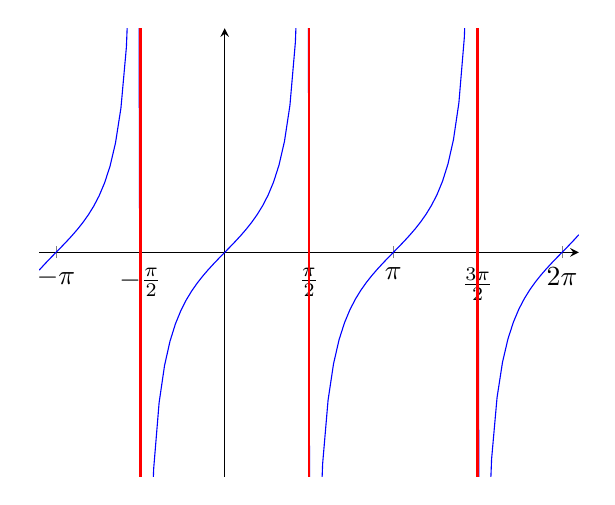
\begin{tikzpicture} 
\begin{axis}[
  axis x line=center, axis y line=center, 
  ymax=4.1,ymin=-4.1, ymajorticks=false,
  xtick={-3.141592654,-1.570796327,1.570796327,3.141592654,4.71238898,6.283185307},
  xticklabels={$-\pi$, $-\frac{\pi}{2}$, $\frac{\pi}{2}$, $\pi$, $\frac{3\pi}{2}$,$2\pi$}
  ]
\addplot[blue,domain=-1.1*pi:2.1*pi,samples=100] {tan(deg(x))}; 

\addplot[line width=1pt,red] coordinates {(-1.570796327,4.15) (-1.570796327,-4.15)};
\addplot[line width=1pt,red] coordinates {(1.570796327,4.15) (1.570796327,-4.15)};
\addplot[line width=1pt,red] coordinates {(4.71238898,4.15) (4.71238898,-4.15)};
\end{axis}
\end{tikzpicture}
\end{tabular}
\end{center}

\section{Trigonometry --- Special Triangles}
\begin{center}
  \includegraphics[height=4cm]{special_triangles}
\end{center}
From the above pair of special triangles we have
\begin{align*}
  \sin \frac{\pi}{4} &= \frac{1}{\sqrt{2}} &  \sin \frac{\pi}{6} &= \frac{1}{2} & \sin \frac{\pi}{3} &= \frac{\sqrt{3}}{2} \\   
  \cos \frac{\pi}{4} &= \frac{1}{\sqrt{2}} &  \cos \frac{\pi}{6} &= \frac{\sqrt{3}}{2} & \cos \frac{\pi}{3} &= \frac{1}{2} \\   
  \tan \frac{\pi}{4} &= 1 &  \tan \frac{\pi}{6} &= \frac{1}{\sqrt{3}} & \tan 
\frac{\pi}{3} &= \sqrt{3}
\end{align*}

\section{Trigonometry --- Simple Identities}
\begin{itemize}
 \item Periodicity
\begin{align*}
  \sin(\theta+2\pi) &= \sin(\theta) &
  \cos(\theta+2\pi) &= \cos(\theta) 
\end{align*}
\item Reflection
\begin{align*}
  \sin(-\theta)&=-\sin(\theta) & \cos(-\theta) &=\cos(\theta) 
\end{align*}
\item Reflection around $\pi/4$
\begin{align*}
\sin\left(\tfrac{\pi}{2}-\theta\right)&=\cos\theta &
\cos\left(\tfrac{\pi}{2}-\theta\right)&=\sin\theta 
\end{align*}
\item Reflection around $\pi/2$
\begin{align*}
\sin\left(\pi-\theta\right)&=\sin\theta &
\cos\left(\pi-\theta\right)&=-\cos\theta 
\end{align*}
\item Rotation by $\pi$
\begin{align*}
\sin\left(\theta+\pi\right)&=-\sin\theta &
\cos\left(\theta+\pi\right)&=-\cos\theta 
\end{align*}
\item Pythagoras
\begin{align*}
\sin^2\theta + \cos^2 \theta &=1  \\
\tan^2\theta + 1  &= \sec^2\theta \\
1 + \cot^2 \theta &=\csc^2\theta
\end{align*}
\item $\sin$ and $\cos$ building blocks
\begin{align*}
\tan\theta=\frac{\sin\theta}{\cos\theta}\qquad
\csc\theta=\frac{1}{\sin\theta}\qquad
\sec\theta=\frac{1}{\cos\theta}\qquad
\cot\theta=\frac{\cos\theta}{\sin\theta}=\frac{1}{\tan\theta}
\end{align*}
\end{itemize}

\section{Trigonometry --- Add and Subtract Angles}\label{sec trig add}
\begin{itemize}
 \item Sine
\begin{align*}
  \sin(\alpha \pm \beta) &= \sin(\alpha)\cos(\beta) \pm \cos(\alpha)\sin(\beta)
  \end{align*}
 \item Cosine
\begin{align*}
  \cos(\alpha \pm \beta) &= \cos(\alpha)\cos(\beta) \mp \sin(\alpha)\sin(\beta)
\end{align*}
\item Tangent
\begin{align*}
\tan(\alpha+\beta)&=\frac{\tan\alpha+\tan\beta}{1-\tan\alpha\tan\beta} \\
\tan(\alpha-\beta)&=\frac{\tan\alpha-\tan\beta}{1+\tan\alpha\tan\beta}
\end{align*}
\item Double angle
\begin{align*}
  \sin(2\theta) &= 2\sin(\theta)\cos(\theta) \\
  \cos(2\theta) &= \cos^2(\theta) - \sin^2(\theta) \\
  &= 2\cos^2(\theta) - 1   \\
  &= 1 - 2\sin^2(\theta) \\
  \tan(2\theta) &= \frac{2\tan(\theta)}{1-\tan^2\theta} \\
\cos^2\theta&=\frac{1+\cos(2\theta)}{2} \\
\sin^2\theta&=\frac{1-\cos(2\theta)}{2} \\
\tan^2\theta&=\frac{1-\cos(2\theta)}{1+\cos(2\theta)}
\end{align*}
\item Products to sums
\begin{align*}
\sin(\alpha)\cos(\beta)&= \frac{\sin(\alpha+\beta) +  \sin(\alpha-\beta)}{2} \\
\sin(\alpha)\sin(\beta)&= \frac{\cos(\alpha-\beta) - \cos(\alpha+\beta)}{2}\\
\cos(\alpha)\cos(\beta)&= \frac{\cos(\alpha-\beta) + \cos(\alpha+\beta)}{2}
\end{align*}
\item Sums to products
\begin{align*}
\sin\alpha+\sin\beta 
           &= 2 \sin\frac{\alpha+\beta}{2}\cos\frac{\alpha-\beta}{2} \\
\sin\alpha-\sin\beta 
           &= 2 \cos\frac{\alpha+\beta}{2}\sin\frac{\alpha-\beta}{2} \\
\cos\alpha+\cos\beta  
           &= 2 \cos\frac{\alpha+\beta}{2}\cos\frac{\alpha-\beta}{2} \\
\cos\alpha-\cos\beta 
           &= -2 \sin\frac{\alpha+\beta}{2}\sin\frac{\alpha-\beta}{2}
\end{align*}

\end{itemize}

\section{Inverse Trigonometric Functions}\label{sec inv trig}
\begin{center}
\renewcommand{\arraystretch}{1.5}
\begin{tabular}{|c|c|c|}
\hline
$\arcsin x$ & $\arccos x$ & $\arctan x$\\
\hline
Domain: $-1 \leq x \leq 1$&
Domain: $-1 \leq x \leq 1$&
Domain: all real numbers\\
Range: $-\frac{\pi}{2} \leq \arcsin x \leq \frac{\pi}{2}$&
Range: $0 \leq \arccos x \leq \pi$&
Range: $-\frac{\pi}{2} < \arctan x < \frac{\pi}{2}$\\
\hline
\begin{tikzpicture} 
\begin{axis}[
  legend pos = north west,
  axis x line=center, axis y line=center, 
  xmax=1.1,xmin=-1.1, xtick={-1,1},
  ymin=-2, ymax=2,
  ytick={-1.570796327,1.570796327},
  yticklabels={$-\nicefrac{\pi}{2}$, $\nicefrac{\pi}{2}$}
  ]
\addplot[blue, line width=1pt, domain=-1:1,samples=100] {asin(x)/180*pi}; 
% \legend{$\arcsin \theta$}
\end{axis}
\end{tikzpicture}
&
%\raisebox{0.15in}{
\begin{tikzpicture} 
\useasboundingbox (0,0) rectangle (5,4.2);
\begin{axis}[
  axis x line=center, axis y line=center, 
  xmax=1.1,xmin=-1.1, xtick={-1,1},
  ymin=-0.3,ymax=3.4,
  ytick={0,1.570796327,3.141592654},
  yticklabels={0,$\nicefrac{\pi}{2}$, $\pi$}
  ]
 \addplot[blue, line width=1pt, domain=-1:1,samples=100] {acos(x)/180*pi}; 
% \legend{$\cos \theta$}
\end{axis}
\end{tikzpicture}
%}
&
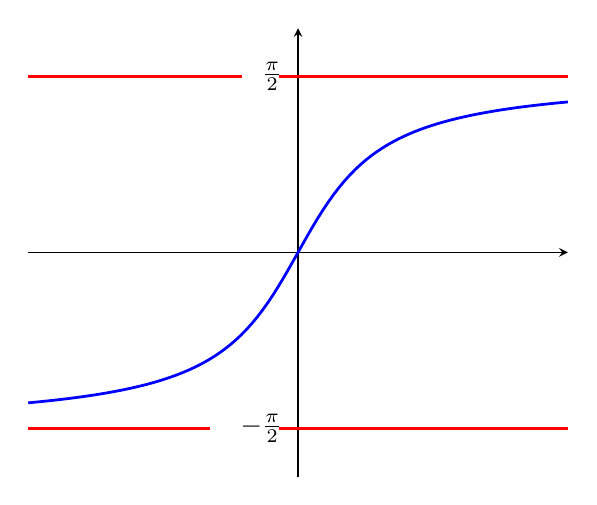
\begin{tikzpicture} 
\begin{axis}[
  legend pos = north west,
  axis x line=center, axis y line=center, 
  xmax=4.3,xmin=-4.3, xmajorticks=false,
  ymin=-2,ymax=2,
  ytick={-1.570796327,1.570796327},
  yticklabels={$-\frac{\pi}{2}$, $\frac{\pi}{2}$}
  ]
\addplot[blue, line width=1pt, domain=-4.3:4.3,samples=100] {atan(x)/180*pi}; 
% \legend{$\tan \theta$}

\addplot[line width=1pt,red] coordinates {(4.3,-1.570796327) (-0.3,-1.570796327)};
\addplot[line width=1pt,red] coordinates {(-1.4,-1.570796327) (-4.3,-1.570796327)};
\addplot[line width=1pt,red] coordinates {(4.3,1.570796327) (-0.3,1.570796327)};
\addplot[line width=1pt,red] coordinates {(-0.9,1.570796327) (-4.3,1.570796327)};
\end{axis}
\end{tikzpicture}
\\ \hline
\end{tabular}
\renewcommand{\arraystretch}{1}
\end{center}
Since these functions are inverses of each other we have
\begin{align*}
  \arcsin(\sin \theta) &= \theta & -\frac{\pi}{2} \leq \theta \leq \frac{\pi}{2} \\
  \arccos(\cos \theta) &= \theta & 0 \leq \theta \leq \pi \\
  \arctan(\tan \theta) &= \theta & -\frac{\pi}{2} < \theta < \frac{\pi}{2}	
\end{align*}
and also
\begin{align*}
  \sin(\arcsin x) &= x & -1 \leq x \leq 1 \\
  \cos(\arccos x) &= x & -1 \leq x \leq 1 \\
  \tan(\arctan x) &= x & \text{any real $x$}
\end{align*}
%The compositions of trignometric and inverse trigonometric functions are
%\begin{align*}
%  \sin( \arcsin x ) &= x & 
%  \sin( \arccos x ) &= \sqrt{1-x^2} & 
%  \sin( \arctan x ) &= \frac{x}{\sqrt{1+x^2}} \\ 
%%
%  \cos( \arcsin x ) &= \sqrt{1-x^2} & 
%  \cos( \arccos x ) &= x &
%  \cos( \arctan x ) &= \frac{1}{\sqrt{1+x^2}} \\ 
%%
%  \tan( \arcsin x ) &= \frac{x}{\sqrt{1-x^2}} & 
%  \tan( \arccos x ) &= \frac{\sqrt{1-x^2}}{x} &
%  \tan( \arctan x ) &= x 
%\end{align*}

\begin{center}
\renewcommand{\arraystretch}{1.5}
\begin{tabular}{|c|c|c|}
\hline
$\arccsc x$ & $\arcsec x$ & $\arccot x$\\
\hline
Domain: $|x|\ge 1$&
Domain: $|x|\ge 1$&
Domain: all real numbers\\
Range: $-\frac{\pi}{2} \leq \arccsc x \leq \frac{\pi}{2}$&
Range: $0 \leq \arcsec x \leq \pi$&
Range: $0 < \arccot x < \pi$\\[-0.1in]
       $\arccsc x \ne 0$ &
       $\arcsec x \ne \frac{\pi}{2}$ &
        \\
\hline
\begin{tikzpicture} 
\begin{axis}[
  legend pos = north west,
  axis x line=center, axis y line=center, 
  xmax=4.3,xmin=-4.3, xtick={-1,1},
  ymin=-2, ymax=2,
  ytick={-1.570796327,1.570796327},
  yticklabels={$-\frac{\pi}{2}\!\!\!$, $\frac{\pi}{2}$}
  ]
\addplot[blue, line width=1pt, domain=1:4.3,samples=50] {asin(1/x)/180*pi}; 
\addplot[blue, line width=1pt, domain=-4.3:-1,samples=50] {asin(1/x)/180*pi}; 
\end{axis}
\end{tikzpicture}
&
\begin{tikzpicture} 
\useasboundingbox (0,0) rectangle (5,4.2);
\begin{axis}[
  axis x line=center, axis y line=center, 
  xmax=4.3,xmin=-4.3, xtick={-1,1},
  ymin=-0.3,ymax=3.4,
  ytick={0,1.570796327,3.141592654},
  yticklabels={0,$\frac{\pi}{2}$, $\pi$}
  ]
 \addplot[blue, line width=1pt, domain=1:4.3,samples=100] {acos(1/x)/180*pi}; 
 \addplot[blue, line width=1pt, domain=-4.3:-1,samples=100] {acos(1/x)/180*pi}; 
% \legend{$\cos \theta$}
\end{axis}
\end{tikzpicture}
&
\begin{tikzpicture} 
\begin{axis}[
  legend pos = north west,
  axis x line=center, axis y line=center, 
  xmax=4.3,xmin=-4.3, xmajorticks=false,
  ymin=-0.3,ymax=3.4,
  ytick={0,1.570796327,3.141592654},
  yticklabels={0,$\frac{\pi}{2}$, $\pi$}
  ]
\addplot[blue, line width=1pt, domain=-4.3:-0.01,samples=100] {atan(1/x)/180*pi + pi}; 
\addplot[blue, line width=1pt, domain=0.01:4.3,samples=100] {atan(1/x)/180*pi}; 
% \legend{$\tan \theta$}

\addplot[line width=1pt,red] coordinates {(4.3,3.141592654) (-0.3,3.141592654)};
\addplot[line width=1pt,red] coordinates {(-0.9,3.141592654) (-4.3,3.141592654)};
\end{axis}
\end{tikzpicture}
\\ \hline
\end{tabular}
\renewcommand{\arraystretch}{1}
\end{center}
Again
\begin{align*}
  \arccsc(\csc \theta) &= \theta & -\frac{\pi}{2} \leq \theta \leq \frac{\pi}{2},\ \theta\ne 0 \\
  \arcsec(\sec \theta) &= \theta & 0 \leq \theta \leq \pi,\ \theta\ne \frac{\pi}{2} \\
  \arccot(\cot \theta) &= \theta & 0 < \theta < \pi	
\end{align*}
and 
\begin{align*}
  \csc(\arccsc x) &= x & |x|\ge 1 \\
  \sec(\arcsec x) &= x & |x|\ge 1 \\
  \cot(\arccot x) &= x & \text{any real $x$}
\end{align*}















\graphicspath{{figures/powerlog/}}
\chapter{Powers and Logarithms}\label{app power log}





\section{Powers}\label{sec powers}
In the following, $x$ and $y$ are arbitrary real numbers,
$q$ is an arbitrary constant that is strictly bigger
than zero and $e$ is 2.7182818284, to ten decimal places.
\begin{itemize}
 \item 
     $e^0=1$,\quad $q^0=1$

\item 
         $e^{x+y}=e^xe^y$,\quad
         $e^{x-y}=\frac{e^x}{e^y}$,\quad
         $q^{x+y}=q^xq^y$,\quad
         $q^{x-y}=\frac{q^x}{q^y}$


\item 
   $e^{-x}=\frac{1}{e^x}$,\quad
   $q^{-x}=\frac{1}{q^x}$

\item 
    $\big(e^x\big)^y=e^{xy}$,\quad
    $\big(q^x\big)^y=q^{xy}$
\item 
    $\diff{\hfill}{x}e^x=e^x$,\quad
    $\diff{\hfill}{x}e^{g(x)}=g'(x)e^{g(x)}$,\quad
    $\diff{\hfill}{x}q^x=(\ln q)\ q^x$
\item
    $\int e^x\ \dee{x}=e^x+C$,\quad
    $\int e^{ax}\ \dee{x}=\frac{1}{a}e^{ax}+C$ if $a\ne 0$
\item
     $e^x =\sum\limits_{n=0}^\infty\frac{x^n}{n!}$
\item    
    $\lim\limits_{x\rightarrow\infty}e^x=\infty$, \quad
    $\lim\limits_{x\rightarrow-\infty}e^x=0$ 

    $\lim\limits_{x\rightarrow\infty}q^x=\infty$, \quad
    $\lim\limits_{x\rightarrow-\infty}q^x=0$ if $q>1$

    $\lim\limits_{x\rightarrow\infty}q^x=0$, \quad
    $\lim\limits_{x\rightarrow-\infty}q^x=\infty$ if $0<q<1$
\item  The graph of $2^x$ is given below. The graph of  $q^x$,
for any $q>1$, is similar.

\begin{center}
\includegraphics{expGraph2.pdf}
\end{center}


\end{itemize}


\section{Logarithms}\label{sec logs}

In the following, $x$ and $y$ are arbitrary real numbers that 
are strictly bigger than 0 (except where otherwise specified), 
$p$ and $q$ are arbitrary constants that are strictly bigger 
than one, and $e$ is 2.7182818284, to ten decimal places.
The notation $\ln x$ means $\log_e x$. Some people use $\log x$
to mean $\log_{10} x$, others use it to mean $\log_e x$ and still
others use it to mean $\log_2 x$.

\begin{itemize}
\item   
       $e^{\ln x}=x$,\quad  
       $q^{\log_q x}=x$
\item 
       $\ln \big(e^x\big)=x$,\quad
       $\log_q \big(q^x\big)=x$\quad for all $-\infty<x<\infty$ 
\item   
        $\log_q x=\frac{\ln x}{\ln q}$,\quad
        $\ln x=\frac{\log_p x}{\log_p e}$,\quad
        $\log_q x=\frac{\log_p x}{\log_p q}$
\item   
          $\ln 1=0$,\quad 
          $\ln e=1$


          $\log_q 1=0$,\quad 
          $\log_q q=1$

\item 
      $\ln(xy)=\ln x+\ln y$,\quad
      $\log_q(xy)=\log_q x+\log_q y$

\item 
     $\ln\big(\frac{x}{y}\big)=\ln x-\ln y$,\quad 
     $\log_q\big(\frac{x}{y}\big)=\log_q x-\log_q y$
 
\item 
     $\ln\big(\frac{1}{y}\big)=-\ln y$,\quad 
     $\log_q\big(\frac{1}{y}\big)=-\log_q y$

\item 
     $\ln(x^y)=y\ln x$,\quad
     $\log_q(x^y)=y\log_q x$

\item
    $\diff{\hfill}{x}\ln x = \frac{1}{x}$,\quad
    $\diff{\hfill}{x}\log_q x = \frac{1}{x\ln q}$

\item
    $\int \ln x\ \dee{x}= x\ln x-x +C$,\quad
    $\int \log_q x\ \dee{x}= x\log_q x-\frac{x}{\ln q} +C$,\quad

\item
    $\lim\limits_{x\rightarrow\infty}\ln x=\infty$,\quad 
           $\lim\limits_{x\rightarrow0}\ln x=-\infty$

    $\lim\limits_{x\rightarrow\infty}\log_q x=\infty$,\quad
           $\lim\limits_{x\rightarrow0}\log_q x=-\infty$ 

\item The graph of $\log_{10} x$ is given below. The graph of  $\log_q x$,
for any $q>1$, is similar.

\begin{center}
\includegraphics{logGraph10.pdf}
\end{center}

\end{itemize}








\chapter{Table of Derivatives}\label{app deriv}

Throughout this table, $a$ and $b$ are constants, independent of $x$.

\begin{center}

\renewcommand{\arraystretch}{2.5}
     \begin{tabular}{|c|c|}
        \hline
    $F(x)$ & $F'(x)=\diff{F}{x}$ \\ 
        \hline\hline
%  linearity 
    $af(x)+bg(x)$ & $af'(x)+bg'(x)$ \\  \hline
    $f(x)+g(x)$ & $f'(x)+g'(x)$ \\  \hline
    $f(x)-g(x)$ & $f'(x)-g'(x)$ \\  \hline
    $af(x)$ & $af'(x)$ \\  \hline
%  product, quotient
    $f(x)g(x)$ & $f'(x)g(x)+f(x)g'(x)$ \\  \hline
    $f(x)g(x)h(x)$ &$f'(x)g(x)h(x)+f(x)g'(x)h(x)+f(x)g(x)h'(x)$ \\  \hline
    $\frac{f(x)}{g(x)}$ & $\frac{f'(x)g(x)-f(x)g'(x)}{g(x)^2}$ \\  \hline
    $\frac{1}{g(x)}$ & $-\frac{g'(x)}{g(x)^2}$ \\  \hline\hline
%  chain
    $f\big(g(x)\big)$ & $f'\big(g(x)\big)g'(x)$ \\  \hline
     \end{tabular}

     \begin{tabular}{|c|c|}
        \hline
    $F(x)$ & $F'(x)=\diff{F}{x}$ \\ 
        \hline\hline
%  powers
%    $1$ & $0$ \\  \hline
    $a$ & $0$ \\  \hline
    $x^a$ & $ax^{a-1}$ \\  \hline
    $g(x)^a$ & $ag(x)^{a-1}g'(x)$ \\  \hline\hline
% trig
    $\sin x$ & $\cos x$ \\  \hline
    $\sin g(x)$ & $g'(x)\cos g(x)$ \\  \hline
    $\cos x$ & $-\sin x$ \\  \hline
    $\cos g(x)$ & $-g'(x)\sin g(x)$ \\  \hline
    $\tan x$ & $\sec^2 x$ \\  \hline
    $\csc x$ & $-\csc x\cot x$ \\  \hline
    $\sec x$ & $\sec x\tan x$ \\  \hline
    $\cot x$ & $-\csc^2 x$ \\  \hline\hline
% exp
    $e^x$ & $e^x$ \\  \hline
    $e^{g(x)}$ & $g'(x)e^{g(x)}$ \\  \hline
    $a^x$ & $(\ln a)\ a^x$ \\  \hline\hline
     \end{tabular}\qquad\qquad
     \begin{tabular}{|c|c|}
        \hline
    $F(x)$ & $F'(x)=\diff{F}{x}$ \\ 
        \hline\hline
%  log
    $\ln x$ & $\frac{1}{x}$ \\  \hline
    $\ln g(x)$ & $\frac{g'(x)}{g(x)}$ \\  \hline
    $\log_a x$ & $\frac{1}{x\ln a}$ \\  \hline\hline
% inverse trig
    $\arcsin x$ & $\frac{1}{\sqrt{1-x^2}}$ \\  \hline
    $\arcsin g(x)$ & $\frac{g'(x)}{\sqrt{1-g(x)^2}}$ \\  \hline
    $\arccos x$ & $-\frac{1}{\sqrt{1-x^2}}$ \\  \hline
    $\arctan x$ & $\frac{1}{1+x^2}$ \\  \hline
    $\arctan g(x)$ & $\frac{g'(x)}{1+g(x)^2}$ \\  \hline
    $\arccsc x$ & $-\frac{1}{|x|\sqrt{x^2-1}}$ \\  \hline
    $\arcsec x$ & $\frac{1}{|x|\sqrt{x^2-1}}$ \\  \hline
    $\arccot x$ & $-\frac{1}{1+x^2}$ \\  \hline
     \end{tabular}
\renewcommand{\arraystretch}{1.0}

\end{center}





\chapter{Table of Integrals}\label{app integral}

Throughout this table, $a$ and $b$ are given constants, independent of $x$
and $C$ is an arbitrary constant.



\begin{center}

\renewcommand{\arraystretch}{2.5}
     \begin{tabular}{|c|c|}
        \hline
    $f(x)$ & $ F(x)=\int f(x)\ \dee{x}$ \\ 
        \hline\hline
$af(x)+bg(x)$ & $a\int f(x)\ \dee{x}+b\int g(x)\ \dee{x}\ +\ C$ \\  \hline
$f(x)+g(x)$ & $\int f(x)\ \dee{x}+\int g(x)\ \dee{x}\ +\ C$ \\  \hline
$f(x)-g(x)$ & $\int f(x)\ \dee{x}-\int g(x)\ \dee{x}\ +\ C$ \\  \hline
$af(x)$ & $a\int f(x)\ \dee{x}\ +\ C$ \\  \hline\hline
%  parts
$u(x)v'(x)$ & $ u(x)v(x)-\int u'(x)v(x)\ \dee{x}\ +\ C$ \\  \hline\hline
%  chain
$f\big(y(x)\big)y'(x)$ & $ F\big(y(x)\big)\hbox{ where }F(y)=\int f(y)\ \dee{y}$ \\  \hline\hline
%  powers
%$1$ & $x+C$ \\  \hline
$a$ & $ax+C$ \\  \hline
$x^a$ & $\frac{x^{a+1}}{a+1}+C\hbox{ if }a\ne-1$ \\  \hline
$\frac{1}{x}$ & $\ln|x|+C$ \\  \hline
$g(x)^ag'(x)$ & $\frac{g(x)^{a+1}}{a+1}+C\hbox{ if }a\ne -1$ \\  \hline\hline
     \end{tabular}

     \begin{tabular}{|c|c|}
        \hline
    $f(x)$ & $ F(x)=\int f(x)\ \dee{x}$ \\ 
        \hline\hline
% trig
$\sin x$ & $-\cos x+C$ \\  \hline
$g'(x)\sin g(x)$ & $-\cos g(x)+C$ \\  \hline
$\cos x$ & $\sin x+C$ \\  \hline
$\tan x$ & $\ln|\sec x|+C$ \\  \hline
$\csc x$ & $\ln |\csc x-\cot x|+C$ \\  \hline
$\sec x$ & $\ln |\sec x+\tan x|+C$ \\  \hline
$\cot x$ & $\ln|\sin x|+C$ \\  \hline
$\sec^2 x$ & $\tan x+C$ \\  \hline
$\csc^2 x$ & $-\cot x+C$ \\  \hline
$\sec x\tan x$ & $\sec x+C$ \\  \hline
$\csc x\cot x$ & $-\csc x+C$ \\  \hline\hline
     \end{tabular}\qquad\qquad
     \begin{tabular}{|c|c|}
        \hline
    $f(x)$ & $ F(x)=\int f(x)\ \dee{x}$ \\ 
        \hline\hline
% exp
$e^x$ & $e^x+C$ \\  \hline
$e^{g(x)}g'(x)$ & $e^{g(x)}+C$ \\  \hline
$e^{ax}$ & $\frac{1}{a}\ e^{ax}+C$ \\  \hline
$a^x$ & $\frac{1}{\ln a}\ a^x+C$ \\  \hline\hline
%  log
$\ln x$ & $x\ln x -x+C$ \\  \hline\hline
% inverse trig
$\frac{1}{\sqrt{1-x^2}}$ & $\arcsin x+C$ \\  \hline
$\frac{g'(x)}{\sqrt{1-g(x)^2}}$ & $\arcsin g(x)+C$ \\  \hline
$\frac{1}{\sqrt{a^2-x^2}}$ & $\arcsin \frac{x}{a}+C$ \\  \hline
$\frac{1}{1+x^2}$ & $\arctan x+C$ \\  \hline
$\frac{g'(x)}{1+g(x)^2}$ & $\arctan g(x)+C$ \\  \hline
$\frac{1}{a^2+x^2}$ & $\frac{1}{a}\arctan \frac{x}{a}+C$ \\  \hline
$\frac{1}{x\sqrt{x^2-1}}$ & $\arcsec x+C$ \quad($x>1$)\\  \hline
     \end{tabular}
\renewcommand{\arraystretch}{1.0}

\end{center}





\chapter{Table of Taylor Expansions}\label{app taylor}


Let $n\ge $ be an integer. Then if the function $f$ has $n+1$ derivatives on an interval that contains both $x_0$ and $x$, we have the Taylor expansion
\begin{align*}
f(x)&=f(x_0)+f'(x_0)\,(x-x_0)+\dfrac{1}{2!}f''(x_0)\,(x-x_0)^2+\cdots
+\dfrac{1}{n!}f^{(n)}(x_0)\,(x-x_0)^n\\ &\hskip0.5in
+\dfrac{1}{(n+1)!}f^{(n+1)}(c)\,(x-x_0)^{n+1}\qquad\hbox{for some $c$ between
$x_0$ and $x$}
\end{align*}
The limit as $n\rightarrow\infty$ gives the Taylor series
\begin{align*}
f(x)&=\sum_{n=0}^\infty\dfrac{f^{(n)}(x_0)}{n!}(x-x_0)^n
\end{align*}
for $f$. When $x_0=0$ this is also called the Maclaurin series for $f$.
Here are Taylor series expansions of some important functions.
\begin{align*}
e^x&=\sum_{n=0}^\infty \dfrac{1}{n!}x^n 
                       &&\text{for $-\infty<x<\infty$}\\
&=1+x+\dfrac{1}{2}x^2+\dfrac{1}{3!}x^3+\cdots+\dfrac{1}{n!}x^n+\cdots
        \hidewidth\\
\sin x&=\sum_{n=0}^\infty\dfrac{(-1)^n}{(2n+1)!}x^{2n+1}
                        &&\text{for $-\infty<x<\infty$} \\
      &=x-\dfrac{1}{3!}x^3+\dfrac{1}{5!}x^5-\cdots
        +\dfrac{(-1)^n}{(2n+1)!}x^{2n+1}+\cdots
        \hidewidth\\
\cos x&=\sum_{n=0}^\infty\dfrac{(-1)^n}{(2n)!}x^{2n}
                      &&\text{for $-\infty<x<\infty$}\\
        &=1-\dfrac{1}{2!}x^2+\dfrac{1}{4!}x^4-\cdots
        +\dfrac{(-1)^n}{(2n)!}x^{2n}+\cdots
             \hidewidth\displaybreak[0]\\
\dfrac{1}{1-x}&=\sum_{n=0}^\infty x^n
                  &&\text{for $-1\le x<1$}\\
              &=1+x+x^2+x^3+\cdots+x^n+\cdots
                  \hidewidth\displaybreak[0]\\
\dfrac{1}{1+x}&=\sum_{n=0}^\infty(-1)^n x^n
                   &&\text{for $-1<x\le 1$}\\
              &=1-x+x^2-x^3+\cdots+(-1)^nx^n+\cdots
                 \hidewidth\displaybreak[0]\\
\ln(1-x)&=-\sum_{n=1}^\infty\dfrac{1}{n}x^n
                 &&\text{for $-1\le x< 1$}\\
        &=-x-\half x^2-\dfrac{1}{3}x^3-\cdots-\dfrac{1}{n}x^n-\cdots
                 \hidewidth\\
\ln(1+x)&=-\sum_{n=1}^\infty\dfrac{(-1)^n}{n}x^n
                    &&\text{for $-1<x\le 1$}\\
        &=x-\half x^2+\dfrac{1}{3}x^3-\cdots-\dfrac{(-1)^n}{n}x^n-\cdots
                      \hidewidth\\
(1+x)^p&=1+px+\dfrac{p(p-1)}{2}x^2+\dfrac{p(p-1)(p-2)}{3!}x^3+\cdots
                     \hidewidth\\   
           &\hskip0.5in+
           \dfrac{p(p-1)(p-2)\cdots(p-n+1)}{n!}x^n+\cdots
                      \hidewidth
\end{align*}



\graphicspath{{figures/coord/}}

%\setcounter{secnumdepth}{0}
\renewcommand{\theequation}{\thechapter.\arabic{equation}}
\renewcommand{\thetheorem}{\thechapter.\arabic{theorem}}
\renewcommand{\thebc}{\thechapter.\arabic{theorem}}
\renewcommand{\theeg}{\thechapter.\arabic{theorem}}
%\counterwithin{theorem}{chapter}
%\numberwithin{theorem}{chapter}


\chapter{3d Coordinate Systems}\label{ap:3dcoord}

\section{Cartesian Coordinates}\label{ap:cartCoord}
Here is a figure showing the definitions of the 
three Cartesian coordinates $(x,y,z)$
\begin{efig}
\begin{center}
    \includegraphics{cart1.pdf}
\end{center}
\end{efig}
and here are three figures showing a surface of constant $x$,
a surface of constant $x$, and a surface of constant $z$.
\begin{wfig}
\begin{center}
    \includegraphics{cart3.pdf}\qquad
    \includegraphics{cart4.pdf}\qquad
    \includegraphics{cart2.pdf}
\end{center}
\end{wfig}
Finally here is a figure showing the volume element $\dee{V}$ in
cartesian coordinates.
\begin{efig}
\begin{center}
    \includegraphics{cart5.pdf}
\end{center}
\end{efig}



\section{Cylindrical Coordinates}\label{ap:cylCoord}

Here is a figure showing the definitions of the 
three cylindrical coordinates 
\begin{align*}
r&=\text{ distance from }(0,0,0)\text{ to }(x,y,0)\\
\theta&=\text{ angle between the the $x$ axis and the line joining $(x,y,0)$ to $(0,0,0)$}\\
z&=\text{ signed distance from }(x,y,z)
\text{ to the $xy$--plane}
\end{align*}
\begin{efig}
\begin{center}
    \includegraphics{cyl1.pdf}
\end{center}
\end{efig}
The cartesian and cylindrical coordinates
are related by
\begin{align*}
x&=r\cos\theta &
y&=r\sin\theta &
z&=z \\
    r&=\sqrt{x^2+y^2} &
    \theta&=\arctan\frac{y}{x} &
    z&=z
\end{align*}
Here are three figures showing a surface of constant $r$,
a surface of constant $\theta$, and a surface of constant $z$.
\begin{wfig}
\begin{center}
    \includegraphics{cyl3.pdf}\qquad
    \includegraphics{cyl4.pdf}\qquad
    \includegraphics{cyl2.pdf}
\end{center}
\end{wfig}
Finally here is a figure showing the volume element $\dee{V}$ in
cylindrical coordinates.
\begin{efig}
\begin{center}
    \includegraphics{cyl5.pdf}
\end{center}
\end{efig}





\section{Spherical Coordinates}\label{ap:spherCoord}

Here is a figure showing the definitions of the 
three spherical coordinates 
\begin{align*}
\rho&=\text{ distance from }(0,0,0)\text{ to }(x,y,z)\\
\varphi&=\text{ angle between the $z$ axis and the line joining $(x,y,z)$ to $(0,0,0)$} \\
\theta&=\text{ angle between the $x$ axis and the line joining $(x,y,0)$ to $(0,0,0)$}
%\varphi&=\text{ angle between the line }\overline{(0,0,0)\,(x,y,z)}
%\text{ and the $z$ axis}\\
%\theta&=\text{ angle between the line }\overline{(0,0,0)\,(x,y,0)}
%\text{ and the $x$ axis}
\end{align*}
\begin{efig}
\begin{center}
    \includegraphics{spherical.pdf}
\end{center}
\end{efig}
and here are two more figures giving the side and top views of the 
previous figure.
\begin{efig}
\begin{center}
    \includegraphics{sphericalSide.pdf}\qquad
    \includegraphics{sphericalTop.pdf}\qquad
\end{center}
\end{efig}
The cartesian and spherical coordinates
are related by
\begin{align*}
x&=\rho\sin\varphi\cos\theta &
y&=\rho\sin\varphi\sin\theta &
z&=\rho\cos\varphi \\
 \rho&=\sqrt{x^2+y^2+z^2} &
 \theta&=\arctan\frac{y}{x} &
 \varphi&=\arctan\frac{\sqrt{x^2+y^2}}{z}
\end{align*}
Here are three figures showing a surface of constant $\rho$,
a surface of constant $\theta$, and a surface of constant $\varphi$.
\begin{wfig}
\begin{center}
    \includegraphics{spher2.pdf}\qquad
    \includegraphics{spher3.pdf}\qquad
    \includegraphics{spher4.pdf}
\end{center}
\end{wfig}
Here is a figure showing the surface element $\dee{S}$ in
spherical coordinates
\begin{efig}
\begin{center}
    \includegraphics{spher11.pdf}
\end{center}
\end{efig}
and two extracts of the above figure to make it easier to see 
how the factors $\rho\ \dee{\varphi}$ and 
$\rho\sin\varphi\ \dee{\theta}$ arise.
\begin{wfig}
\begin{center}
    \includegraphics{spher9.pdf}\qquad
    \includegraphics{spher10.pdf}
\end{center}
\end{wfig}
Finally, here is a figure showing the volume element $\dee{V}$ in
spherical coordinates
\begin{efig}
\begin{center}
    \includegraphics{spher5.pdf}
\end{center}
\end{efig}
%and two extracts of the above figure to make it easier to see 
%how $\rho\ \dee{\varphi}$ and $\rho\sin\varphi\ \dee{\theta}$ arise.
%\begin{wfig}
%\begin{center}
%    \includegraphics{spher6.pdf}\qquad
%    \includegraphics{spher7.pdf}
%\end{center}
%\end{wfig}





\graphicspath{{figures/ISO/}}

%\setcounter{secnumdepth}{0}
\renewcommand{\theequation}{\thechapter.\arabic{equation}}
\renewcommand{\thetheorem}{\thechapter.\arabic{theorem}}
\renewcommand{\thebc}{\thechapter.\arabic{theorem}}
\renewcommand{\theeg}{\thechapter.\arabic{theorem}}
%\counterwithin{theorem}{chapter}
%\numberwithin{theorem}{chapter}


\chapter{ISO Coordinate System Notation}\label{ap:ISO}

In this text we have chosen symbols for the various polar, cylindrical and 
spherical coordinates that are standard for mathematics. There is 
another, different, set of symbols that are commonly used in the 
physical sciences and engineering. Indeed, there is an international convention, called ISO 80000-2, that specifies those symbols\footnote{It specifies more than just those symbols. See \url{https://en.wikipedia.org/wiki/ISO_31-11}
and \url{https://en.wikipedia.org/wiki/ISO/IEC_80000}. The full
ISO 80000-2 is available at \url{https://www.iso.org/standard/64973.html} --- for \$\$.}. In this appendix, we summarize the definitions and standard properties of the polar, cylindrical and spherical coordinate systems using the
ISO symbols.   

\section{Polar Coordinates}\label{ap:ISOpolar}
In the ISO convention the symbols $\rho$ and $\phi$ are used 
(instead of $r$ and $\theta$) for polar coordinates.
\begin{align*}
\rho&=\text{ the distance from }(0,0)\text{ to }(x,y)\\
\phi&=\text{ the (counter-clockwise) angle between the $x$ axis 
               and the line joining $(x,y)$ to $(0,0)$}
\end{align*}
\begin{efig}
\begin{center}
    \includegraphics{polar.pdf}
\end{center}
\end{efig}
Cartesian and polar coordinates are related by
\begin{align*}
x&=\rho\cos\phi &
y&=\rho\sin\phi  \\
    \rho&=\sqrt{x^2+y^2} &
    \phi&=\arctan\frac{y}{x}
\end{align*}
The following two figures show a number of lines of constant $\phi$,
on the left, and curves of constant $\rho$, on the right.
\begin{efig}
\begin{center}
    \includegraphics{polarTh.pdf}\qquad\qquad
    \includegraphics{polarR.pdf}
\end{center}
\end{efig}


Note that the polar angle $\phi$ is only defined up to integer multiples
of $2\pi$. For example, the point $(1,0)$ on the $x$-axis could have 
$\phi=0$, but could also have $\phi=2\pi$ or $\phi=4\pi$. It is sometimes
convenient to assign $\phi$ negative values. When $\phi<0$, the
counter-clockwise angle $\phi$ refers to the clockwise angle $|\phi|$. 
For example, the point $(0,-1)$ on the negative $y$-axis can have $\phi=-\frac{\pi}{2}$ and can also have $\phi=\frac{3\pi}{2}$.
\begin{efig}
\begin{center}
    \includegraphics{polarNegTh.pdf}
\end{center}
\end{efig}



It is also sometimes convenient to extend the above definitions by saying that
$x=\rho\cos\phi$ and $y=\rho\sin\phi$ even when $\rho$ is negative. For example,
the following figure shows $(x,y)$ for $\rho=1$, $\phi=\nicefrac{\pi}{4}$
and for $\rho=-1$, $\phi=\nicefrac{\pi}{4}$.
\vadjust{
\begin{efig}
\begin{center}
    \includegraphics{polarNeg.pdf}
\end{center}
\end{efig}
}
Both points lie on the  line through the origin that makes an angle of
$45^\circ$ with the $x$-axis and both are a distance one from the origin.
But they are on opposite sides of the the origin.

The area element in polar coordinates is
\begin{equation*}
\dee{A} = \rho\,\dee{\rho}\,\dee{\phi}
\end{equation*}
\begin{efig}
\begin{center}
    \includegraphics{polarA.pdf}
\end{center}
\end{efig}





\section{Cylindrical Coordinates}\label{ap:ISOcylCoord}
In the ISO convention the symbols $\rho$, $\phi$ and $z$ are used 
(instead of $r$, $\theta$ and $z$) for cylindrical coordinates.
\begin{align*}
\rho&=\text{ distance from }(0,0,0)\text{ to }(x,y,0)\\
\phi&=\text{ angle between the the $x$ axis and the line joining $(x,y,0)$ to $(0,0,0)$}\\
z&=\text{ signed distance from }(x,y,z)
\text{ to the $xy$-plane}
\end{align*}
\begin{efig}
\begin{center}
    \includegraphics{cyl1.pdf}
\end{center}
\end{efig}
The cartesian and cylindrical coordinates
are related by
\begin{align*}
x&=\rho\cos\phi &
y&=\rho\sin\phi &
z&=z \\
    \rho&=\sqrt{x^2+y^2} &
    \phi&=\arctan\frac{y}{x} &
    z&=z
\end{align*}
Here are three figures showing a surface of constant $\rho$,
a surface of constant $\phi$, and a surface of constant $z$.
\begin{wfig}
\begin{center}
    \includegraphics{cyl3.pdf}\qquad
    \includegraphics{cyl4.pdf}\qquad
    \includegraphics{cyl2.pdf}
\end{center}
\end{wfig}
Finally here is a figure showing the volume element $\dee{V}$ in
cylindrical coordinates.
\begin{efig}
\begin{center}
    \includegraphics{cyl5.pdf}
\end{center}
\end{efig}

\section{Spherical Coordinates}\label{ap:ISOspherCoord}

In the ISO convention the symbols $r$ (instead of $\rho$), 
$\phi$ (instead of $\theta$) and $\theta$ (instead of $\phi$) are used 
for spherical coordinates.
\begin{align*}
r&=\text{ distance from }(0,0,0)\text{ to }(x,y,z)\\
\theta&=\text{ angle between the $z$ axis and the line joining $(x,y,z)$ to $(0,0,0)$} \\
\phi&=\text{ angle between the $x$ axis and the line joining $(x,y,0)$ to $(0,0,0)$}
\end{align*}
\begin{efig}
\begin{center}
    \includegraphics{spherical.pdf}
\end{center}
\end{efig}
Here are two more figures giving the side and top views of the 
previous figure.
\begin{efig}
\begin{center}
    \includegraphics{sphericalSide.pdf}\qquad
    \includegraphics{sphericalTop.pdf}\qquad
\end{center}
\end{efig}
The cartesian and spherical coordinates
are related by
\begin{align*}
x&=r\sin\theta\cos\phi &
y&=r\sin\theta\sin\phi &
z&=r\cos\theta \\
 r&=\sqrt{x^2+y^2+z^2} &
 \phi&=\arctan\frac{y}{x} &
 \theta&=\arctan\frac{\sqrt{x^2+y^2}}{z}
\end{align*}
Here are three figures showing a surface of constant $r$,
a surface of constant $\phi$, and a surface of constant $\theta$.
\begin{wfig}
\begin{center}
    \includegraphics{spher2.pdf}\qquad
    \includegraphics{spher3.pdf}\qquad
    \includegraphics{spher4.pdf}
\end{center}
\end{wfig}
Finally, here is a figure showing the volume element $\dee{V}$ in
spherical coordinates
\begin{efig}
\begin{center}
    \includegraphics{spher5.pdf}
\end{center}
\end{efig}
and two extracts of the above figure to make it easier to see 
how $r\ \dee{\theta}$ and $r\sin\theta\ \dee{\phi}$ arise.
\begin{wfig}
\begin{center}
    \includegraphics{spher6.pdf}\qquad
    \includegraphics{spher7.pdf}
\end{center}
\end{wfig}





\graphicspath{{figs_quadric/}}

%\setcounter{secnumdepth}{0}
\renewcommand{\theequation}{\thechapter.\arabic{equation}}
\renewcommand{\thetheorem}{\thechapter.\arabic{theorem}}
\renewcommand{\thebc}{\thechapter.\arabic{theorem}}
\renewcommand{\theeg}{\thechapter.\arabic{theorem}}
%\counterwithin{theorem}{chapter}
%\numberwithin{theorem}{chapter}


\chapter{Conic Sections and Quadric Surfaces}\label{ap:quadric}

A conic section is the curve of intersection of a cone and a plane
that does not pass through the vertex of the cone.
This is illustrated in the figures below.
\vadjust{
\begin{efig}
\begin{center}
    \includegraphics{conePlaneCircle.pdf}\quad
    \includegraphics{conePlaneEllipse.pdf}\quad
    \includegraphics{conePlaneParabola.pdf}\quad
    \includegraphics{conePlaneHyperbola.pdf}
\end{center}
\end{efig}
}
An equivalent\footnote{It is outside our scope to prove this equivalence.} 
(and often used) definition is that a conic section is the set of all points  
in the $xy$--plane that obey $Q(x,y)=0$ with
\begin{equation*}
Q(x,y) = Ax^2 + By^2 + Cxy + Dx + Ey + F =0
\end{equation*}
being a polynomial of degree two\footnote{Technically, we should also require
that the constants $A$, $B$, $C$, $D$, $E$, $F$, are real numbers,
that $A$, $B$, $C$ are not all zero, that $Q(x,y)=0$ has more than one 
real solution, and that the polynomial can't be factored
into the product of two polynomials of degree one.}.
By rotating and translating  our coordinate system the equation of the conic section can be brought
into one of the forms\footnote{This statement can be justified using a 
linear algebra eigenvalue/eigenvector analysis. It is 
beyond what we can cover here, but is not too difficult for a standard 
linear algeba course.}
\begin{itemize}
\item
$\al x^2 + \be y^2 =\ga$ with $\al,\be,\ga >0$, which is an ellipse
(or a circle),
\item
$\al x^2 - \be y^2 =\ga$ with $\al,\be>0$, $\ga\ne0$, which is a hyperbola,
\item 
$x^2 = \delta y$, with $\delta\ne 0$ which is a parabola.
\end{itemize}
\goodbreak

The three dimensional analogs of conic sections, surfaces 
in three dimensions given by quadratic equations, are called quadrics.
An example is the sphere $x^2+y^2+z^2=1$. Here are some tables giving
all of the quadric surfaces.

%\bigskip
\vfill
\noindent
\renewcommand{\arraystretch}{1.5}
\begin{tabular}{ | c | c | c | c | c |}
  \hline
  name & \parbox[c]{1.8cm}{\smallskip elliptic\\cylinder}
       & \parbox[c]{1.8cm}{\smallskip parabolic\\cylinder} 
       & \parbox[c]{1.8cm}{\smallskip hyperbolic\\cylinder} 
       & sphere \\[0.1in]
  \hline
  \parbox[c]{2.75cm}{\smallskip equation in\\standard form} 
             & $\frac{x^2}{a^2}+\frac{y^2}{b^2}=1$
             & $y=ax^2$ 
             & $\frac{x^2}{a^2}-\frac{y^2}{b^2}=1$
             & $x^2+y^2+z^2=r^2$\\[0.1in]
  \hline
  \parbox[c]{2.75cm}{\smallskip $x=$ constant \\cross--section} 
            & two lines 
            & one line 
            & two lines 
            & circle \\[0.1in]
  \hline
  \parbox[c]{2.75cm}{\smallskip $y=$ constant \\cross--section} 
            & two lines
            & two lines
            & two lines 
            & circle \\[0.1in]
  \hline
  \parbox[c]{2.75cm}{\smallskip $z=$ constant \\cross--section} 
            & ellipse
            & parabola 
            & hyperbola 
            & circle \\[0.1in]
  \hline
  sketch 
     & \raisebox{-45pt}[42pt][52pt]
              { \smash{\includegraphics[scale=1.3]{cylinder.pdf}} }
     & \raisebox{-47pt}[42pt][52pt]
             {\smash{\includegraphics[scale=1.3]{parabolic_cylinder.pdf}}}
     & \raisebox{-50pt}[42pt][52pt]
             {\smash{\includegraphics[scale=1.4]{hyperbolic_cylinder.pdf}}}
     & \raisebox{-47pt}[42pt][52pt]
              { \smash{\includegraphics[scale=1.3]{sphere.pdf}} }
      \\[0.1in]
  \hline
\end{tabular}
\vfill
%\bigskip\medskip
\noindent
\begin{tabular}{ | c | c | c | c | c |}
  \hline
  name & ellipsoid 
       & \parbox[c]{1.8cm}{\smallskip elliptic\\paraboloid}
       & \parbox[c]{1.5cm}{\smallskip elliptic\\cone}  \\[0.1in]
  \hline
  \parbox[c]{2.75cm}{\smallskip equation in\\standard form} 
       & \parbox[c]{3.4cm}{\ \ \ \ 
             $\frac{x^2}{a^2}+\frac{y^2}{b^2}+\frac{z^2}{c^2}=1$} 
       & \parbox[c]{3.4cm}{\ \ \ \ \ 
             $\frac{x^2}{a^2}+\frac{y^2}{b^2}=\frac{z}{c}$}
       & \parbox[c]{2.3cm}{
             $\frac{x^2}{a^2}+\frac{y^2}{b^2}=\frac{z^2}{c^2}$} \\[0.1in]
  \hline
  \parbox[c]{2.75cm}{\smallskip $x=$ constant \\cross--section} 
            & ellipse
            & parabola
            & \parbox[c]{3.5cm}{\smallskip two lines if $x=0$\\
                                           hyperbola if $x\ne 0$}   \\[0.1in]
  \hline
  \parbox[c]{2.75cm}{\smallskip $y=$ constant \\cross--section} 
            & ellipse
            & parabola
            & \parbox[c]{3.5cm}{\smallskip two lines if $y=0$\\
                                           hyperbola if $y\ne 0$} \\[0.1in]
  \hline
  \parbox[c]{2.75cm}{\smallskip $z=$ constant \\cross--section} 
            & ellipse
            & ellipse 
            & ellipse  \\[0.1in]
  \hline
  sketch 
     & \raisebox{-50pt}[45pt][55pt]
              { \smash{\includegraphics[scale=1.5]{ellipsoid.pdf}} }
     & \raisebox{-48pt}[45pt][55pt]
              { \smash{\includegraphics[scale=1.3]{elliptic_paraboloid.pdf}} }
     & \raisebox{-48pt}[45pt][55pt]
              { \smash{\includegraphics[scale=1.4]{cone.pdf}} }
      \\[0.1in]
  \hline
\end{tabular}
\vfill\newpage

%\bigskip\bigskip
\noindent
\begin{tabular}{ | c | c | c | c | c |}
  \hline
  name &\parbox[c]{2.75cm}{\smallskip hyperboloid\\of one sheet} 
       & \parbox[c]{2.75cm}{\smallskip hyperboloid\\of two sheets}
       & \parbox[c]{2.1cm}{\smallskip hyperbolic\\paraboloid}  \\[0.1in]
  \hline
  \parbox[c]{2.75cm}{\smallskip equation in\\standard form} 
       & \parbox[c]{3.4cm}{\ \ \ \ 
             $\frac{x^2}{a^2}+\frac{y^2}{b^2}-\frac{z^2}{c^2}=1$} 
       & \parbox[c]{3.4cm}{\ \  
             $\frac{x^2}{a^2}+\frac{y^2}{b^2}-\frac{z^2}{c^2}=-1$} 
       & \parbox[c]{2.1cm}{
             $\frac{y^2}{b^2}-\frac{x^2}{a^2}=\frac{z}{c}$} \\[0.1in]
  \hline
  \parbox[c]{2.75cm}{\smallskip $x=$ constant \\cross--section} 
            & hyperbola
            & hyperbola
            & parabola  \\[0.1in]
  \hline
  \parbox[c]{2.75cm}{\smallskip $y=$ constant \\cross--section} 
            & hyperbola
            & hyperbola
            & ellipse \\[0.1in]
  \hline
  \parbox[c]{2.75cm}{\smallskip $z=$ constant \\cross--section} 
            & ellipse
            & ellipse 
            & \parbox[c]{3.5cm}{\smallskip two lines if $z=0$\\
                                           hyperbola if $z\ne 0$}  \\[0.1in]
  \hline
  sketch 
     & \raisebox{-48pt}[42pt][52pt]
              { \smash{\includegraphics[scale=1.4]{hyperboloid1.pdf}} }
     & \raisebox{-48pt}[42pt][52pt]
              { \smash{\includegraphics[scale=1.4]{hyperboloid2.pdf}} }
     & \raisebox{-46pt}[42pt][52pt]
              { \smash{\includegraphics[scale=1.3]{hyperbolic_paraboloid.pdf}} }
      \\[0.1in]
  \hline
\end{tabular}







\printIssueCount
\end{document}
